\documentclass[11pt,a4paper]{article}
\usepackage[T1]{fontenc}
\usepackage[utf8]{inputenc}
\usepackage[italian]{babel}
\usepackage{lmodern}
\usepackage{amsmath,amssymb,mathtools}
\usepackage{graphicx}
\usepackage{float}
\usepackage{booktabs}
\usepackage{array}
\usepackage{enumitem}
\usepackage{geometry}
\usepackage{microtype}
\usepackage{xcolor}
\usepackage{hyperref}
\usepackage{caption}
\usepackage{longtable}
\usepackage{fancyhdr}
\geometry{margin=2.3cm}
\hypersetup{colorlinks=true,linkcolor=blue!45!black,citecolor=blue!45!black,urlcolor=blue!45!black,pdftitle={Causalita, luce ed espansione cosmologica - Working Paper v1.03}}
\setlength{\parindent}{0pt}
\setlength{\parskip}{0.55em}
\setlength{\headheight}{14pt}
\setlist{nosep,leftmargin=*}
\pagestyle{fancy}
\fancyhf{}
\lhead{Working Paper v1.03}
\rhead{Ipotesi $c+c$}
\cfoot{\thepage}
\newcommand{\LCDM}{\ensuremath{\Lambda\mathrm{CDM}}}
\newcommand{\Gly}{\mathrm{Gly}}
\newcommand{\Gyr}{\mathrm{Gyr}}
\newcommand{\status}[1]{\textsf{#1}}

\title{\textbf{Causalita, luce ed espansione cosmologica}\\
\large Esplorazione cumulativa dell'intuizione ``$c+c$'', di due fotoni co-propaganti e degli orizzonti cosmologici}
\author{Pietro Risi (idea e direzione concettuale)\\ChatGPT, OpenAI (supporto matematico e redazionale)\\\small Autorialita provvisoria per il quaderno di lavoro; da rivedere prima di una eventuale pubblicazione}
\date{\textbf{ERRATA XL--IR} -- Working Paper cumulativo v1.03, 13 ottobre 2026}

\begin{document}
\maketitle

\begin{abstract}
Questo documento raccoglie in forma cumulativa una linea di esplorazione nata dall'intuizione informale che l'espansione cosmologica o la propagazione della prima luce potessero contenere una struttura interpretabile come ``$c+c$''. L'idea e stata progressivamente separata in due rami: (i) la comparsa di termini $2c$ nella cinematica di fronti luminosi e di scale cosmologiche; (ii) l'evoluzione della distanza tra due fotoni emessi in epoche differenti ma propagantisi nella stessa direzione. L'analisi in geometria FLRW mostra che, per un raggio luminoso radiale, la distanza propria soddisfa $\dot D=HD\pm c$; per due raggi co-propaganti i termini luminosi si cancellano e la loro separazione soddisfa $\dot{\Delta D}=H\Delta D$, mentre per due raggi opposti compare $HD+2c$. Il raggio di Hubble soddisfa invece $\dot R_H=c(1+q)$, per cui $\dot R_H=2c$ durante un'era puramente radiativa. Si introduce inoltre $\alpha=HR_p/c$ per l'orizzonte delle particelle, ottenendo l'identita esatta $q=(1-d\alpha/d\ln a)/\alpha$. Il Gate R8 confronta inoltre orizzonte delle particelle, raggio di Hubble, orizzonte apparente ed event horizon. Nel caso spazialmente piatto $R_A=R_H$ e quindi $\alpha=R_p/R_A$. Applicando la termodinamica standard all'orizzonte apparente si recuperano le equazioni di Friedmann, ma non si determina da sola l'equazione di stato della materia: la chiusura dinamica di $\alpha(t)$ resta quindi non derivata. Si introduce anche $\varepsilon=R_e/R_A$, con le identita speculari $\alpha'=1-q\alpha$ e $\varepsilon'=-1-q\varepsilon$. Il Gate R10 deriva poi una mappa generale tra una legge entropica $S(A)$ dell'orizzonte apparente e una Friedmann modificata. Entropie di potenza costante e correzioni logaritmiche falliscono come chiusure minime capaci di conservare le ere standard e produrre da sole l'accelerazione tardiva; una forma tipo Renyi produce invece una transizione a una debole accelerazione di potenza, ma costituisce una classe gia nota e non una conseguenza dell'intuizione $c+c$. Il Gate R11 sottopone quindi a controllo tre possibili principi informazionali: Landauer a saturazione si riduce esattamente alla relazione di Clausius gia usata; la saturazione del bound di Bekenstein ricostruisce la prima Friedmann sotto ipotesi molto forti ma non determina la pressione; l'holographic equipartition di Padmanabhan ricostruisce l'equazione di accelerazione ma importa esplicitamente $\rho+3p$. Nessuno dei tre chiude autonomamente $\alpha(t)$. Il Gate R12 testa quindi la forma dimensionalmente naturale $\rho_X\propto L^{-2}$ su diverse scale causali. Il particle horizon produce un fluido tracker e, se assunto come sorgente totale a saturazione, blocca $\alpha$ a una costante: non genera ne transizioni ne accelerazione. Il cutoff apparente/Hubble e tautologico nel caso totale, mentre il future event horizon puo accelerare ma introduce informazione globale sul futuro. Una densita basata sull'eta conforme evita quest'ultimo problema e puo diventare dominante tardivamente, ma coincide con la classe gia nota della new agegraphic dark energy e richiede un principio microfisico addizionale; non segue dalla saturazione del particle horizon proprio. Viene inoltre testata una chiusura simmetrica passato--futuro, che interpola da $q=1$ a $q=-1$ ma non possiede una lunga era materiale. Il Gate R12b mostra poi che $\eta^{-2}$ non puo essere selezionata dalla sola struttura causale FLRW: sotto la liberta di normalizzazione $a\to\lambda a$, il tempo conforme scala come $\eta\to\eta/\lambda$, mentre $R_p=ac\eta$ resta invariante. Ne segue un ulteriore no-go ristretto: una densita passata costruita senza nuove scale come $\rho_cF(\alpha,\alpha',q,\ldots)$ mantiene una frazione costante in una esatta era di potenza e non puo diventare dominante durante una lunga era materiale senza informazione fisica aggiuntiva. Il Gate R12c introduce allora una sola nuova lunghezza $L_*$ e classifica la famiglia monomiale passata $\rho_X\propto L_*^{n-2}R_p^{-n}$. Per $n<2$ il tracking viene effettivamente rotto; $n=0$ riduce a una costante cosmologica, mentre il primo termine genuinamente causale, $n=1$, produce un attrattore accelerato $a\propto t^2$ ma coincide con il caso $\delta=3/2$ della Tsallis holographic dark energy con particle horizon. La nuova scala sposta quindi il problema: consente il takeover tardivo, ma non seleziona ne l'esponente ne il valore di $L_*$. Il Gate R12d testa allora due ingredienti alternativi: un'interazione covariante tra materia e componente causale e una memoria retarded costruita con operatori covarianti. Per la densita standard $R_p^{-2}$ si ricava l'identita $\Omega_p'/\Omega_p=2(q-1/\alpha)$, che implica $\Omega_p'<0$ durante ogni fase accelerata: un'interazione puo rendere negativa la pressione efficace, ma l'accelerazione non e prodotta da un takeover del particle horizon e richiede una funzione di scambio $Q$ non selezionata dalla causalita. Una memoria dimensionale minimale, come $-\Box U=1$, produce invece $U\propto t^2$ nelle ere di potenza e torna a tracciare $H^2$; memorie adimensionali secolari come $-\Box^{-1}R$ possono rompere il tracking, ma per diventare dinamica richiedono ancora una funzione di distorsione o una nuova scala, come nelle note classi di gravita non locale. Il Gate R12e torna quindi direttamente alla congruenza nulla della ``prima luce'': la Raychaudhuri ottica riproduce la combinazione derivativa di Friedmann, ma dipende da $\rho+p$ ed e cieca a un termine di vuoto $p=-\rho$ o, equivalentemente, a $\Lambda g_{\mu\nu}$. Integrata con la conservazione, la dinamica resta determinata solo fino a una costante cosmologica; inoltre, nel caso piatto, un raggio uscente posto istantaneamente su $R_A=c/H$ soddisfa esattamente $\dot R_+=2c$, mentre il raggio entrante ha $\dot R_-=0$ e l'orizzonte stesso si muove a $c(1+q)$. Il Gate R12f testa infine causal diamond/entanglement equilibrium, gravita unimodulare, vincoli globali sul quattro-volume e la proposta causal-set Everpresent $\Lambda$. I primi tre non selezionano un valore unico senza dati globali o boundary conditions aggiuntive; il ramo causal-set produce invece la scala stocastica $\Lambda_{\rm rms}\sim V_4^{-1/2}$. Per una era piatta $a\propto t^p$ viene derivato esattamente $V_4=\pi c^4t^4/[(1+p)(3+p)(1+3p)]$, da cui $\Lambda_{\rm rms}c^2/H^2=\mathrm{costante}$: il meccanismo e un tracker stocastico e richiede microstruttura discreta e una ampiezza non ancora derivata. Il Gate R12g prende sul serio questa microstruttura senza imporre omogeneita: in un toy model in cui gli stessi elementi causali forniscono contributi aleatori condivisi, la covarianza tra due valori locali e fissata dal quattro-volume di sovrapposizione dei rispettivi passati causali. Ne segue $\mathrm{Corr}[\Lambda(x),\Lambda(y)]=V_4(P_x\cap P_y)/\sqrt{V_4(P_x)V_4(P_y)}$; per eventi annidati sulla stessa worldline, nelle ere di potenza, $\mathrm{Corr}=(t_1/t_2)^2$, mentre in Minkowski a tempo uguale si ottiene il kernel esatto $1-x+x^3/4-x^4/16$ per $x=d/(cT)\le2$. La geometria del passato seleziona quindi una struttura di correlazione non banale senza un kernel fenomenologico, ma non elimina il parametro di ampiezza e soprattutto non fornisce una sorgente locale conservata: una $\Lambda(x)g_{\mu\nu}$ variabile e incompatibile con Bianchi se la materia e separatamente conservata. Il Gate R12h mostra che la conservazione puo essere ripristinata in piu modi inequivalenti: una proiezione trasversa retarded fornisce un tensore conservato ma introduce un operatore nonlocale, una Green function e boundary conditions; un completamento a fluido efficace conserva separatamente la materia al prezzo di abbandonare $p=-\rho$; un vero vuoto stocastico mantiene $p=-\rho$ ma forza uno scambio energia--momento con gli altri settori. Inoltre il kernel di overlap di R12g ha una cuspide lineare all origine: il campo grezzo non e differenziabile in media quadratica, per cui una equazione locale con $\partial_\nu\Lambda$ richiede coarse-graining o una interpretazione stocastica/distribuzionale. Il Gate R12i passa quindi direttamente a un rumore tensoriale $\Xi_{\mu\nu}$ conservato. In spazio piatto, per un modo non nullo, la parte simmetrica e trasversa ammette almeno i due settori indipendenti spin--2 e spin--0, con noise kernel $\widetilde N=A P^{(2)}+B P^{(0)}$: il kernel scalare di overlap puo fissare un inviluppo comune, ma non seleziona il rapporto tra i due settori. Un toy di causal set ``marcato'' fattorizza infatti il volume di overlap da una covarianza tensoriale microscopica indipendente. La stochastic gravity fornisce il benchmark corretto: il noise kernel e conservato perche deriva da un vero operatore energia--impulso, quindi la struttura tensoriale viene dalla microfisica e non dalla sola geometria causale. Il Gate R12j testa infine se una azione stocastica causale e una identita di Ward possano eliminare tale liberta. La risposta e parziale: la diffeomorphism invariance rende la conservazione automatica soltanto per gradi di liberta dinamici on-shell (non per uno scalare casuale esterno), mentre al secondo ordine lascia indipendenti i form factor trasversi spin--2 e spin--0. Le azioni causal-set di Benincasa--Dowker--Glaser forniscono un importante benchmark per il primo cumulante, il cui limite medio riproduce Einstein--Hilbert piu termini di bordo, ma il settore delle fluttuazioni non e fissato dal valore medio e richiede ancora microdinamica; inoltre lo smearing necessario a controllare le fluttuazioni introduce una scala di nonlocalita. Il Gate R12k affronta quindi direttamente il secondo cumulante dell'azione BDG. La letteratura recente ha costruito una decomposizione esatta della varianza in termini di correlazioni tra intervalli causali, ma l'asintotica esplicita in Minkowski/FLRW resta ancora da valutare. Nel quaderno viene derivato un criterio di matching indipendente dai dettagli: se $\mathrm{Var}(S_{\rm BDG})\propto N^\gamma$, una interpretazione Everpresent richiede necessariamente $\gamma=1$, cioe un secondo cumulante estensivo. Lo smearing noto introduce inoltre una nonlocality scale $\ell_k>\ell$; a scala fisica $\ell_k$ fissata le fluttuazioni Poisson coarse-grained si spengono nel limite continuo, mentre mantenere finita una sorgente stocastica richiede una legge di running/critical scaling non ancora derivata. I programmi di coarse-graining causal-set esistenti forniscono un linguaggio RG, ma non selezionano ancora dinamicamente la mesoscale. Il documento registra derivazioni, controlli numerici, rami falliti, questioni aperte e una roadmap per verificare se causalita, orizzonti e termodinamica possano fornire una chiusura indipendente senza inserire $H(t)$ a mano.
 Il Gate R12l separa infine la varianza cinematica da sprinkling dalla varianza dinamica del path sum: nel benchmark dei 2d-orders il finite-size scaling con $\bar\beta=\beta N$ porta a $\mathrm{Var}(S)\sim N^2$ nella fase continuum-like, $N^3$ nella fase cristallina e $N^4$ al picco di coesistenza di primo ordine, quindi nessuno dei regimi termodinamici noti seleziona il requisito $\gamma=1$ trovato in R12k. Questi esponenti non possono tuttavia essere trasferiti automaticamente alla misura Lorentziana $e^{iS}$: i risultati analitici del path sum mostrano soppressione di ampie classi non-manifold-like, ma non calcolano ancora il secondo cumulante quantistico nel settore manifold-like. La selezione dinamica di uno scaling estensivo resta quindi aperta. Il Gate R12m congela quindi un protocollo numerico prima dei risultati e ne esegue un pilot riproducibile: un controllo sintetico recupera $\gamma=0.993$ con intervallo bootstrap contenente $1$, mentre il benchmark fixed-$N$ di sprinkling fornisce $\gamma_{\rm spr}=1.857$ e il benchmark Gibbs continuum-like a $\bar\beta=20$ fornisce $\gamma_{\rm G}=1.637$; entrambi respingono il target estensivo preregistrato. Il risultato Gibbs non viene identificato con il cumulante Lorentziano $\gamma_Q$, che resta non misurato. Il Gate R12n accede quindi direttamente alla misura oscillante mediante exact enumeration del benchmark 2d representation-weighted per $N=4,\ldots,10$: viene costruita senza binning la density of states sui vettori di abbondanze degli intervalli e calcolata a 80 cifre la characteristic function $\phi_N(g)=N!^{-1}\sum_C e^{igS_C}$. Al coupling preregistrato $g=1$ il sign problem resta mild sulla griglia esatta, con $\min|\phi_N|=0.7775$, e il modulo del secondo cumulante connesso produce $\gamma_Q^{\rm rep}=1.1807$ ($R^2=0.9932$), con entrambi i fit di stabilita agli endpoint compatibili con il target estensivo. La classificazione congelata e pertanto \texttt{CONSISTENT\_WITH\_EXTENSIVE\_REP}. Il risultato e tuttavia small-$N$, 2d e representation-weighted: non autorizza a identificare $\gamma_Q^{\rm rep}$ con il path sum causale 4d non etichettato, e R13 resta bloccato. Il Gate R12o valida quindi un estimatore Lorentziano Monte Carlo direttamente contro la DOS esatta a $N=8,9,10$ e lo estende, con un milione di permutazioni indipendenti per taglia, fino a $N=64$. Il replay passa con errori sub-percentuali, ma il problema di fase emerge rapidamente: i quality gate restano soddisfatti soltanto fino a $N=24$, mentre a $N=32$ l'incertezza di $|\kappa_2|$ supera la soglia congelata e da $N=48$ l'average phase non e piu statisticamente risolto. Sulla finestra affidabile $N=12$--$24$ le pendenze locali risultano tutte superestensive ($1.61$--$1.93$), ma il protocollo richiede almeno sei taglie valide e vieta quindi un fit primario di $\gamma$. R12o chiude come \texttt{FINITE\_SIZE\_OR\_SIGN\_INCONCLUSIVE}: il segnale small-$N$ di R12n non viene confermato ne respinto asintoticamente, e il blocker diventa esplicitamente il sign problem Lorentziano. Il Gate R12p testa allora, con protocollo congelato prima dei risultati, una ricostruzione cumulante della characteristic function: $\log\phi(g)=\sum_n\kappa_n(ig)^n/n!$. Il metodo riproduce la DOS esatta a $N=8$--$10$ e il direct-MC fino a $N=20$, ma a $N=24$ la ricostruzione primaria $K=10$ sbaglia il cumulante connesso di circa il $65\%$ e le troncature $K=8,10,12$ non convergono. Il gate chiude quindi \texttt{CE\_METHOD\_VALIDATION\_FAIL} e, come preregistrato, nessuna estensione a $N\ge32$ viene autorizzata. Il sign problem e stato trasformato in un problema di convergenza della serie, non risolto.
Il Gate R12q passa quindi a una ricostruzione globale flat-histogram della density of states: quattro repliche Wang--Landau per taglia, seguite da una produzione multicanonica che accumula la fase ai valori effettivi dell'azione. Quando la stopping rule viene raggiunta, la DOS ricostruisce sia $\phi$ sia $\kappa_2$ con errori tipicamente sub-percentuali o di pochi punti percentuali fino a $N=24$. Tuttavia la robustezza preregistrata fallisce: solo $2/4$ repliche convergono a $N=9$ e $1/4$ a $N=12$, contro il minimo congelato di $3/4$. R12q chiude pertanto \texttt{DOS\_METHOD\_VALIDATION\_FAIL}; nessun $N>24$ viene campionato. Il fallimento e algoritmico e localizzato nella schedule di flatness, non nella precisione della DOS una volta convergente, e motiva il successivo test histogram-free LLR. Il Gate R12r testa quindi una ricostruzione LLR histogram-free della pendenza $d\log\rho/dS$ in finestre sovrapposte, con schedule Robbins--Monro congelata dopo soli development pilot esclusi dal gate ($N=6,7$). L'exact validation si arresta fail-closed: $N=8$ supera le soglie con due repliche valide su tre, ma $N=9$ e $N=10$ producono una sola replica valida su tre, sotto il minimo preregistrato di due. Le singole ricostruzioni valide restano numericamente vicine alla DOS esatta, ma la robustezza non e sufficiente. R12r chiude quindi \texttt{LLR\_METHOD\_VALIDATION\_FAIL}; direct validation ed estensione $N>24$ non vengono eseguite. Il Gate R12s sostituisce le hard windows con umbrella armoniche sovrapposte, replica exchange e reweighting MBAR senza binning della fase. L exact replay $N=8$--$10$ passa con tre repliche valide su tre e errori sub-percentuali; la direct validation passa a $N=12,16,20$ ma fallisce fail-closed a $N=24$, dove dopo il consistency gate restano due repliche valide e gli errori complessi sono $5.84\%$ su $\phi$ e $15.33\%$ su $\kappa_2$, appena oltre le soglie congelate $5\%$ e $15\%$. R12s chiude pertanto \texttt{R12S\_METHOD\_VALIDATION\_FAIL}; nessun $N>24$ viene eseguito.
Il Gate R12t sostituisce il reweighting globale con una decomposizione indipendente per strati dell'azione: probabilita degli strati e momenti complessi condizionati vengono stimati da stream uniformi separati e ricombinati soltanto alla fine. Exact $N=8$--$10$ e direct $N=12$--$24$ passano tutte le soglie preregistrate; l'estensione e quindi autorizzata. A $N=32$ restano due repliche coerenti su tre, ma a $N=40$ ne resta una e a $N=48,64$ nessuna. Il protocollo richiede almeno cinque taglie utili, incluse almeno tre di estensione, mentre ne sopravvivono soltanto $N=20,24,32$: nessun esponente viene fittato e R12t chiude \texttt{R12T\_FINITE\_SIZE\_OR\_PRECISION\_INCONCLUSIVE}. Il Gate R12u testa quindi control variates costruite direttamente sulla rappresentazione di Lehmer della permutazione. L'indipendenza esatta dei digit permette di centrare main effects e interazioni adiacenti con media nulla nota, mantenendo l'estimatore dei momenti complessi non distorto. Exact $N=8$--$10$ e direct $N=12$--$24$ passano integralmente, ma il guadagno di varianza decade monotonicamente e scompare a $N\simeq32$: soltanto una replica $N=32$ supera il quality gate e nessuna fra $N=40,48,64$ sopravvive. R12u chiude quindi \texttt{R12U\_FINITE\_SIZE\_OR\_PRECISION\_INCONCLUSIVE} senza fit di un nuovo esponente. Il Gate R12v deriva infine la cost law della cancellazione complessa per la misura positiva: l'average phase diretto ha relative MSE esatta $(1-|\phi|^2)/(M|\phi|^2)$ e la delta-method di $\kappa_2$ eredita la stessa amplificazione, moltiplicata da un shape factor crescente. Le incertezze R12o seguono queste previsioni; a $N=40$ un target del $15\%$ su $\kappa_2$ richiede gia circa $1.15\times10^8$ campioni iid equivalenti. Inoltre $-2\log|\phi|/\mathrm{Var}_0(S)=0.89$--$0.98$ sul range $N=12$--$40$, mostrando che la severita e in larga parte governata dalla varianza ordinaria dell'azione. Il risultato e una efficiency frontier per gli stimatori direct-like, non un no-go universale su rappresentazioni strutturate. Il Gate R12w passa quindi dalla riduzione di varianza alla struttura globale della distribuzione positiva dell'azione. Un nuovo holdout indipendente mostra, sul range $N=24$--$64$, $\mathrm{Var}(S)\propto N^{2.004}$ e una quasi-collassante legge scalata $X_N=(S-4)/N$; ne segue l'identita $\phi_N(g)=e^{4ig}\widehat f_N(gN)$, che trasforma il target fisso $g=1$ in un problema di Fourier ad alta frequenza. Un surrogate massimo-entropia sestico, scelto in development e validato su holdout freschi, riproduce exact $N=8$--$10$ e direct $N=12$--$24$ sulla finestra numerica implementata, ma nell'estensione resta affidabile soltanto fino a una frequenza standardizzata $t=g\sigma_S$ di ordine $2$. R12x sottopone quindi a audit proprio la continuazione complessa: $9/33$ fit sviluppano massimi reali remoti dominanti fuori dalla quadratura e, piu in generale, gli stessi primi sei momenti consentono fasi ad alta frequenza quasi arbitrarie anche sul supporto osservato. La precedente etichetta di ``global rate model'' viene pertanto ritirata: restano validi lo scaling reale, il quasi-collasso e la finestra Fourier verificata, ma non una topologia saddle/Stokes derivata dal sestico. Il prossimo ramo passa alla teoria large-deviation dei permutons per verificare se l'azione BDG ammetta un limite funzionale combinatorio non arbitrario.


Il Gate R12y sottopone infine a controllo un possibile limite funzionale dell'azione BD rispetto alla topologia debole dei permutons. Due famiglie di permutazioni sono costruite in modo deterministico con lo stesso limite di permuton uniforme, ma con differenti limiti di azione normalizzata $S_\epsilon/N$ al parametro storico $\epsilon=0.21$: $1.2409008855\ldots$ contro $0.5766428695\ldots$. Le identita esatte degli intervalli e il confronto indipendente con il codice storico escludono quindi una chiusura globale basata sul solo permuton, anche al punto a rate function entropica nulla. Rimangono non dimostrate una legge limite per le permutazioni tipiche e una LDP congiunta che includa la microstruttura degli intervalli; l'analisi Lorentziana e il Gate R13 restano bloccati.


Il Gate R12z mostra che il profilo degli intervalli del benchmark uniforme richiede una compensazione: per ogni $k$ fissato, $\mathbb E[N_k]/N=\ln N+\gamma_E-H_k-2+o(1)$, mentre i coefficienti dell'azione soddisfano due cancellazioni esatte. Ne deriva, per tutte le taglie $N\ge2$, l'identita $\mathbb E[S_N]=4[1-(1-\epsilon)^N]$ a $\epsilon=0.21$, senza fit. L'enumerazione esatta fino a $N=7$ e nuovi campioni indipendenti fino a $N=256$ verificano la formula; gli errori di troncatura del profilo \emph{centrato} sono piccoli soltanto sulle taglie testate. Una LDP congiunta, la tightness delle code compensate e una teoria della fase Lorentziana restano non dimostrate; R13 rimane bloccato.


Il Gate R12aa deriva una riformulazione esatta dell'azione mediante la seconda differenza discreta del profilo di intervalli: se $g_k=\binom{k+2}{2}(1-\epsilon)^k$, allora $\sum_k f_kN_k=\sum_k g_k(N_k-2N_{k+1}+N_{k+2})$. La media della curvatura discreta converge punto per punto a $1/[(k+1)(k+2)]$, nonostante la deriva logaritmica dei conteggi grezzi. Si dimostra un cutoff $K_N=O(\log N)$ con errore che tende uniformemente a zero su tutte le permutazioni per $S_N/N$, ma anche un no-go deterministico per qualunque cutoff fisso $K$. Una nuova verifica esaustiva $N=2$--$8$ e campionamenti congelati $N=64$--$1024$ passano i controlli; il calo osservato della dispersione normalizzata impedisce di estendere come universale il fit R12w limitato a $N=24$--$64$. Tightness in probabilita, distribuzione limite, LDP congiunta e settore oscillante rimangono aperti; R13 resta bloccato.


Il Gate R12ab ricava una formula esatta, a $N$ finito, per le covarianze dei conteggi di intervalli di una permutazione uniforme: le finestre posizionali disgiunte sono indipendenti, mentre quelle sovrapposte richiedono una funzione generatrice condizionata agli estremi. L'enumerazione completa fino a $N=8$ e un calcolo indipendente delle probabilita congiunte fino a $N=6$ superano i controlli. Si ottiene inoltre un criterio matematico: la concentrazione in $L^2$ dell'azione normalizzata e equivalente all'annullamento asintotico di una forma quadratica di covarianza troncata a $K_N=O(\ln N)$, con errore di coda uniformemente controllato. Holdout indipendenti fino a $N=1024$ mostrano covarianze decrescenti, ma non forniscono un bound asintotico: la concentrazione, la LDP congiunta e il path sum fisico restano aperti. R13 rimane bloccato.



Il Gate R12ac chiude finalmente il criterio lasciato aperto da R12ab per la misura positiva delle permutazioni uniformi 2d: una rappresentazione tramite $N$ punti indipendenti nel quadrato, una stima di influenza per risampling e la disuguaglianza di Efron--Stein forniscono il limite superiore rigoroso $\operatorname{Var}(S_N)=O_\epsilon(N(1+\ln N)^2)$. Quindi $(S_N-\mathbb ES_N)/N\to0$ in $L^2$ e $Q_{N,K_N}\to0$ per ogni cutoff logaritmico del gate precedente. A cardinalita fissata si dimostra inoltre concentrazione dei conteggi dopo ricentraggio della deriva $\ln N$ e del profilo di seconde differenze attorno alla sua media limite. Si tratta esclusivamente del benchmark positivo 2d \emph{representation-weighted}: non risolve il sign problem Lorentziano, non determina un esponente asintotico ottimale, non prova una large-deviation principle congiunta e non abilita il Gate R13.



Il Gate R12ad usa il bound Efron--Stein di R12ac per derivare una finestra rigorosa della funzione caratteristica positiva:
$|e^{-ig\mathbb E_0S_N}\phi_N(g)-1|\le g^2\operatorname{Var}_0(S_N)/2$,
che forza la fase centrata a 1 soltanto se $g_N=o((\sqrt N(1+\ln N))^{-1})$; non fornisce alcun controllo a $g=1$ fissato.
Un protocollo indipendente e congelato prima della produzione misura $\operatorname{Var}_0(S_N)$ fino a $N=2048$, con enumerazione esatta $N=3$--$8$ e confronto con la DOS storica $N=8$--$10$. Le pendenze log--log finite diminuiscono al crescere della finestra, ma non selezionano un esponente asintotico. La fase diretta a $g=1$ viene classificata statisticamente risolta soltanto a $N=16,24$ da un disco di confidenza simultaneo al 99\%; non e risolta a taglie superiori. La scala sharp delle fluttuazioni e la fisica Lorentziana 4d restano aperte e R13 non e autorizzato.


Il Gate R12ae ricava una formula esplicita a dimensione finita per la prima proiezione Hoeffding--ANOVA dell'azione del benchmark 2d positivo, includendo sia le coppie per cui il punto marcato e un estremo sia quelle il cui intervallo lo contiene. Per punti iid uniformi nel quadrato si ottiene rigorosamente $\mathrm{Var}_0(S_N)\ge N\mathbb E[h_{1,N}^2]>0$ a ogni $N\ge2$. La formula supera enumerazioni complete fino a $N=8$, controlli numerici ad alta precisione e simulazioni condizionate prospettiche. Il contributo di primo ordine confrontato con la varianza campionaria storica rappresenta circa il $9.35\%$ a $N=16$, il $6.71\%$ a $N=64$ e il $3.24\%$ a $N=128$. Questi rapporti finite-$N$ non dimostrano alcuna legge asintotica: il problema della fluttuazione residua, le proiezioni di ordine superiore, la fase a coupling fisso e il path sum 4d rimangono aperti. R13 resta bloccato.


Il Gate R12af estende la decomposizione Hoeffding dell'azione positiva 2d al secondo ordine. Con i due punti marcati, i contributi in cui entrambi si trovano internamente allo stesso rettangolo sono inclusi in una formula finita esatta per $h_{2,N}$. La scomposizione $\mathrm{Var}(S_N)=N\mathbb E h_{1,N}^2+\binom N2\mathbb E h_{2,N}^2+\mathrm{Var}(R_{\ge3,N})$ segue dall'ortogonalita delle proiezioni. Tutte le verifiche preregistrate (30/30) passano. Fra $N=16$ e $N=48$, i primi due ordini spiegano circa 67--76\% della varianza campionaria storica a dimensione finita; la scala del residuo, il comportamento asintotico e la fase a coupling fisso non vengono determinati. Il Gate R12ag e il prossimo; R13 resta bloccato.



Il Gate R12ag introduce infine la terza proiezione Hoeffding--ANOVA nel benchmark positivo 2d: una formula esatta finite-$N$ per $h_{3,N}$ conserva i casi di tre marcati interni ai rettangoli. Trentuno controlli prospettici su trentuno passano, mentre stime QMC a $N=3,4,8,16,32$ misurano un terzo contributo di varianza significativo nelle taglie finite. Una quarta differenza mista non nulla, calcolata con aritmetica razionale per $N=4$, dimostra $P_{4,4}>0$. Nessuna legge asintotica sharp della varianza, soluzione del problema Lorentziano o nuova chiusura cosmologica e stata derivata: R13 resta bloccato.


Il Gate R12ah introduce un certificato esatto per l'intero residuo Hoeffding di ordine almeno quattro usando una copia dei punti che conserva ciascun punto con probabilita $p$ e risampiona altrimenti. La covarianza di tale accoppiamento e $C_N(p)=\sum_{r=1}^{N} p^r P_{r,N}$ e la semi-differenza quadratica media e $D_N(p)=\sum_r(1-p^r)P_{r,N}$. Per $p=1/2$, sottraendo i tre contributi bassi si deriva $B_N\le V_{\ge4,N}\le16B_N/15$ per le aspettative esatte a ogni $N$; le versioni plug-in con Monte Carlo restano approssimazioni. Centoventicinque controlli preventivi passano, ma i nuovi valori puntuali non riconciliano integralmente le vecchie stime per differenza; nessuna dominanza asintotica dei primi tre ordini e dimostrata. In conseguenza del punto di verifica strategico viene sospesa l'estensione automatica del ramo matematico 2d e pianificato R12ai, dedicato ai prerequisiti di un ponte fisico Lorentziano 4d conservato. R13 rimane bloccato.


Il Gate R12ai sospende l'estensione automatica del toy 2d e sottopone a controllo il ponte fisico 4d. Un risultato costruttivo limitato mostra che il kernel di sovrapposizione dei passati causali e semidefinito positivo e, su Minkowski, la tensorizzazione $\Xi_{\mu\nu}=(\partial_\mu\partial_\nu-\eta_{\mu\nu}\Box)\phi$ e conservata in senso distribuzionale e possiede noise kernel positivo su funzioni di prova. Ma per un campo omogeneo non genera densita di energia e la covariantizzazione attraverso $F R$ lascia $\nabla^\mu\mathcal A_{\mu\nu}=-R\partial_\nu F/2$ se $F$ e esterno. La misura Lorentziana causal-set 4d, una sorgente dinamica on-shell e il suo settore di risposta non sono derivati; R13 resta bloccato. R12aj richiedera una definizione esplicita del candidato microdinamico, senza fit cosmologico.


Il Gate R12aj definisce un candidato BDG 4d con misura oscillante su un diamante Minkowski a numero di punti fissato. La formula esatta per $N=2$ e 1693 controlli preregistrati passano. Il campionamento a $g=1$ non risolve statisticamente la fase per $N=16,32,64$. Tuttavia la misura importa il background e non definisce una dinamica gravitazionale autonoma: operatore energia--impulso, Ward on-shell, noise/risposta retarded e limite continuo non sono derivati. R13 rimane bloccato.

Il Gate R12ak affronta infine il blocco di selezione della misura: a parita di azione BDG 4d, due distribuzioni finite entrambe invarianti sotto rietichettatura (uniforme sugli ordini etichettati oppure sulle classi di isomorfismo) producono ampiezze oscillanti differenti. Il controesempio $N=2$ e analitico, e l'enumerazione esaustiva $N=1,\ldots,5$ ne verifica l'estensione finita. Il risultato e un no-go ristretto per la selezione mediante la sola simmetria, non un no-go universale sulla causal set quantum gravity: uno stato/somma su storie 4d, la Ward on-shell, il rumore e la risposta retarded e il limite continuo non sono derivati. Si chiude R12ak come audit e si mantiene R13 bloccato.

Il Gate R12al esamina un candidato microdinamico indipendente e preesistente, la crescita sequenziale classica per percolazione transitiva. Essa soddisfa le condizioni classiche note ma dipende da un parametro $p$ non selezionato dalle simmetrie; gia a $N=2$ due valori danno un'ampiezza diagnostica BDG diversa. Per ogni $p\in(0,1)$ fisso il rapporto d'ordine soddisfa il bound $\mathbb E(1-r_N)\le 2(1-p)/[p^2(N-1)]$ e converge a uno in probabilita, in contrasto con il valore $1/10$ dei diamanti piatti Minkowski 4d. Si tratta di una esclusione limitata alla baseline classica con $p$ fisso, NON di un no-go sulla gravita quantistica causale. Nessuna misura quantistica, Ward gravitazionale, risposta o dinamica cosmologica indipendente e stata derivata; R13 resta bloccato.


Il Gate R12am riprende condizionalmente la complex sequential growth gia nota nella letteratura: con ampiezze $z^{L}(1-z)^{I}$ e un funzionale di decoerenza rank-one, le condizioni quantistiche dei cilindri a $N$ finito sono soddisfatte per intere famiglie di $z$ complessi. Due scelte preregistrate danno misure differenti gia per $N=2$; il principio non seleziona la misura. Una moltiplicazione terminale per la fase BDG rompe inoltre la consistenza dei cilindri per genitori diversi, senza un fattore globale di normalizzazione sufficiente. I risultati non decidono l'estensione sulla sigma-algebra infinita, non realizzano quantum Bell causality operatoriale non commutativa e non forniscono una dinamica 4d conservata. R13 resta BLOCCATO.

Il Gate R12an studia quindi la normalizzazione locale delle transizioni dopo l'inserimento della fase BDG: i cilindri tornano consistenti, ma due storie naturalmente etichettate di uno stesso poset a tre elementi ricevono ampiezze differenti per i due parametri preregistrati. Una funzione di partizione finita calcolata a ritroso ripristina consistenza e invarianza a $H$ fissato, ma la risposta dipende dal bordo futuro scelto. Non emerge una regola microfisica passata-only; il Gate R13 rimane bloccato.

Il Gate R12ao chiude ora il controllo sul riaggiustamento armonico della fase BDG: poiche la differenza di azione e un cobordo esatto, l'operatore di trasferimento deformato e coniugato a quello di crescita complessa non deformato. Una correzione armonica che normalizzi i cilindri elimina esplicitamente la fase dal trasferimento e richiede una funzione ulteriore non selezionata. La soluzione costante recupera la dinamica di partenza; un controesempio a orizzonte finito dimostra la non unicita senza cambiare $z$ o $g$. I due replay confermano 2404/2404 e 2463/2463 controlli, rispettivamente. La struttura e un risultato algebrico noto applicato al nostro toy, non una chiusura gravitazionale 4d. R13 resta bloccato.\par
\par Il Gate R12ap completa un controllo rimasto aperto in R12am: la percolazione complessa scalare e coerente sui cilindri finiti, ma, per entrambi i parametri storici non reali, non ammette una misura complessa finita numerabilmente additiva sulla sigma-algebra completa delle storie naturalmente etichettate. La partizione per relazioni fra nascite consecutive ha variazione totale esatta $V_N=(|z|+|1-z|)^{N-1}$, divergente per $z\notin[0,1]$. Il criterio e verificato da due enumerazioni indipendenti, e si tratta di un ostacolo di estensione noto nella letteratura, non di un no-go sulla sotto-algebra covariante o su tutta la crescita quantistica 4d. La chiusura cosmologica resta non derivata e R13 rimane bloccato.

\par Il Gate R12aq affronta infine la liberta residua su una algebra di eventi realmente
covarianti: la famiglia $D_\lambda(A,B)=(1-\lambda)P(A\cap B)+\lambda P(A)P(B)$
e fortemente positiva, normalizzata, consistente e sigma-additiva separatamente
per ogni $\lambda\in[0,1]$, ma produce interferenze differenti perfino fissando
tutti i marginali $D(A,\Omega)=P(A)$. L'evento causale intrinseco ``unico elemento
minimale'' ha probabilita limite non banale in percolazione transitiva,
$r(p)=\prod_{j\ge1}[1-(1-p)^j]$. I due audit esatti (3357 e 70 controlli)
passano; questo e un teorema elementare di non-selezione, non una teoria
quantistica gravitazionale. Nessun ingrediente 4d, sorgente Ward, risposta
retarded, limite continuo o $H(t)$ viene derivato. R13 resta bloccato.


Il Gate R12ar verifica infine se composizione tensoriale di sistemi
indipendenti e purezza restringano la non-unicita di R12aq: la stessa
miscela globale $D_\lambda$ non e chiusa sotto prodotti per valori interni
di $\lambda$, ma il prodotto tensoriale positivo esiste per ogni valore;
imporre purezza seleziona $\lambda=1$ solamente a probabilita di base
$P$ gia fissata. Due differenti $P$ su un evento intrinseco restano
ammissibili: il principio microfisico gravitazionale e la chiusura
cosmologica non sono derivati.
\par Il checkpoint documentale R12as (v0.49) confronta QSG, CDT 4d e gravita stocastica CTP. Un controllo Ward continuo per campo scalare su FLRW viene verificato simbolicamente in due modi, ma non seleziona la misura causale o la microdinamica gravitazionale. Nessun candidato esaminato soddisfa simultaneamente misura, azione, sorgente on-shell, risposta retarded e limite 4d nello stesso spazio di storie: R12as fisico NON AUTORIZZATO, R13 BLOCCATO.\par
Il checkpoint R12at (v0.50) esamina infine l'operatore d'Alembertiano
retarded 4d noto dalla causal set theory. La variazione di una azione
quadratica reale a campo singolo impone la parte simmetrica del kernel e
non riproduce la risposta puramente retarded, salvo il caso degenere di
assenza di relazioni. Un funzionale raddoppiato di tipo Schwinger--Keldysh
risolve formalmente tale ostacolo, ma non determina il noise kernel ne
la misura quantistica o il limite gravitazionale 4d. Il test algebrico
su 5230 poset naturalmente etichettati passa; R13 resta bloccato.\par
\par\smallskip Il controllo R12au usa una microdinamica quantistica libera in quattro dimensioni su sfondo fisso: la risposta retarded e il rumore derivano dalla medesima Hamiltoniana e da uno stato specificato. Per uno stesso modo, il vuoto e uno stato termico producono identica risposta ma rumori diversi, provando la dipendenza dallo stato. Il benchmark non seleziona ne la misura su geometrie dinamiche ne la sorgente gravitazionale; R12as fisico e R13 restano bloccati.\par

\par\smallskip R12av estende il benchmark di materia su sfondo fisso dal noise del campo al correlatore connesso \emph{tensoriale} dell'energia--impulso. In una regolarizzazione a sette modi su $\mathbb{R}\times\mathbb{T}^3$, la positivita e la Ward on-shell sono verificate con un metodo gaussiano e un replay indipendente Fock (400 confronti). Vuoto e stato termico danno stress noise diversi senza modificare l'azione; tuttavia il cutoff rompe la microcausalita esatta, non e stato rimosso, e nessuna misura quantistica delle geometrie dinamiche e stata selezionata. R12as fisico non autorizzato e R13 bloccato.\par
\par\smallskip R12aw sottopone a un controllo UV separato il campo libero dello stesso benchmark: con osservabili del campo distribuiti su supporti spazialmente separati si ottiene un limite del commutatore $O(K^{-6})$, mentre la varianza puntuale del pezzo Wick-quadratico $:\!(\partial_t\phi)^2\!:$ diverge come $\Theta(K^8)$. Una media temporale gaussiana assegnata rende convergente la varianza di quel solo pezzo, con bound rigoroso di troncamento. Non e una costruzione del tensore stress completo e covariantemente rinormalizzato, ne un progresso sulla misura quantistica delle geometrie o su $H(t)$.\par
\par\smallskip R12ax esamina inoltre una relazione ternaria necessaria di Bell causale quantistico per gli operatori di crescita, gia studiata nella letteratura del 2026. Una famiglia esatta di matrici positive non commutative soddisfa quel solo vincolo: si dimostra quindi che esso, isolato, non seleziona ne una dinamica quantistica completa ne la storia cosmologica. Due implementazioni razionali indipendenti superano 372/372 verifiche ciascuna. Restano non derivati la misura quantistica delle geometrie 4D, la sorgente gravitazionale, la risposta metrica e il limite continuo. R12as fisico non autorizzato, R13 bloccato.\par

\par\smallskip R12ay verifica una ulteriore ipotesi di compatibilita fra la somma operatoriale di Markov per le ampiezze e la condizione Kraus di conservazione della traccia, quando vengono imposte agli stessi operatori. Sotto positivita si dimostra un no-go condizionale: soltanto proiettori ortogonali, incompatibili con tutti i rami non singolari; a due rami generali gli operatori risultano commutanti, mentre un controesempio razionale a cinque rami dimostra che l'ostacolo non e universale senza ipotesi. Questo non seleziona una dinamica QSG o una gravita 4d; R13 resta bloccato.

\par\smallskip R12az verifica un principio gia noto per selezionare uno stato di materia libera su un causal set finito: la parte spettrale positiva del commutatore $i\Delta$ secondo Sorkin--Johnston. Con l'operatore retarded finito R12at come input, la funzione a due punti e positiva e realizza la relazione di commutazione; un controesempio analitico su catene di due e tre elementi dimostra tuttavia che la selezione SJ non commuta automaticamente con la restrizione causale, pur essendo invariato il commutatore della sottoregione. La prescrizione richiede propagatore e misura gia specificati, e non seleziona lo stato quantistico della geometria ne una legge cosmologica. R12as fisico resta non autorizzato e R13 bloccato.
\par\smallskip\noindent\textbf{Aggiornamento v0.57:} lo screening R12ba confronta il progetto con la dinamica geometrica 4d gia studiata nelle triangolazioni dinamiche causali (CDT). Nell'ensemble con quattro-volume esattamente fissato, il coupling cosmologico bare $\kappa_4$ non e identificabile da osservabili normalizzate; quando il volume fluttua la sensibilita e proporzionale alla covarianza con $N_4$. La forma euclidea normalizzata $\cos^3$ di de Sitter non fissa autonomamente la scala geometrica. Nessun trasferimento della misura CDT a causal-set QSG, nessuna $\Lambda$ fisica prevista e nessuna nuova $H(t)$ derivata. \textbf{R13 BLOCCATO.}

\par\smallskip Il controllo R12bb collega la difficolta combinatoria delle geometrie causal-set con la distinzione tra fase media e contributo totale: in un sottoinsieme esattamente sommabile di ordini bipartiti etichettati, la prima decade come $|\cos(\theta/2)|^{mn}$, ma la somma non normalizzata cresce al coupling diagnostico storico. La misura positiva a volume libero con solo peso $e^{-\kappa N}$ e non normalizzabile sull'intero insieme dei poset. Sono benchmark ristretti gia motivati da letteratura esistente, non una misura geometrica quantistica completa; R13 rimane BLOCCATO.
\end{abstract}

\vspace{0.5em}
\noindent\textbf{Stato del documento.} Quaderno di ricerca esplorativo, non peer-reviewed. Le equazioni marcate come identita o risultati standard sono distinte dalle ipotesi e dai rami ancora aperti. I risultati numerici sono illustrativi e dipendono dal modello cosmologico scelto.

\begingroup\linespread{0.947}\selectfont
\tableofcontents
\endgroup
\newpage

\section{Origine dell'idea e regola metodologica}

L'intuizione iniziale e stata formulata in modo volutamente semplice: ``l'Universo si espande a $c+c$''. Prima di attribuirle un significato fisico, l'idea e stata usata come stimolo per calcolare quali quantita cosmologiche possano effettivamente assumere un tasso $2c$ senza violare la relativita.

Successivamente l'idea originale e stata precisata. Il punto centrale non era tanto che l'intero Universo possedesse un bordo che si espande a $2c$, quanto il seguente esperimento mentale: un raggio luminoso primordiale viaggia a $c$; molto piu tardi viene emesso un secondo raggio, allineato con il primo e nella stessa direzione, da una regione ormai molto distante. Il secondo raggio ``insegue'' il primo, che e partito molto prima. La domanda diventa quindi: come evolve la loro separazione in un Universo in espansione?

La regola metodologica adottata e:
\begin{quote}
Non salvare l'ipotesi a forza. Distinguere cio che e una conseguenza standard della relativita da cio che sarebbe una predizione nuova. Registrare anche i rami che falliscono.
\end{quote}

\section{Assunzioni geometriche minime}

Per la parte cinematica si usa una metrica FLRW in coordinata radiale comovente $\chi$:
\begin{equation}
 ds^2=-c^2dt^2+a^2(t)\left[d\chi^2+S_k^2(\chi)d\Omega^2\right],
\end{equation}
dove $a(t)$ e il fattore di scala e
\begin{equation}
 H(t)=\frac{\dot a}{a}
\end{equation}
e il parametro di Hubble. Per un raggio luminoso radiale, $ds^2=0$, quindi
\begin{equation}
 \frac{d\chi}{dt}=\pm\frac{c}{a(t)}.
 \label{eq:null_comoving}
\end{equation}

Per una separazione radiale comovente $\Delta\chi$, la distanza propria sulla stessa ipersuperficie di tempo cosmico e
\begin{equation}
 D(t)=a(t)\Delta\chi.
\end{equation}
Queste definizioni sono standard; per una rassegna delle distanze cosmologiche si veda Hogg \cite{Hogg1999}.

\subsection{Una correzione concettuale essenziale}

Un fotone non possiede un sistema di riferimento inerziale di riposo. Non e quindi lecito descrivere un secondo fotone come emesso da un ``sistema che gia viaggia a $c$'' e poi sommare galileanamente $c+c$. La composizione relativistica delle velocita,
\begin{equation}
 u=\frac{u'+v}{1+u'v/c^2},
\end{equation}
restituisce $u=c$ quando $u'=c$ per qualunque $|v|<c$. Il significato eventuale di $c+c$ deve dunque provenire da un'altra quantita: separazioni, orizzonti o crescita geometrica, non dalla velocita locale di un singolo fotone.

\section{Primo ramo: ``l'Universo si espande a $2c$''}

\subsection{Interpretazione con un raggio globale}

Se si imponesse un raggio $R(t)$ tale che
\begin{equation}
 \dot R=c,
\end{equation}
allora un diametro $D=2R$ soddisferebbe $\dot D=2c$. Tuttavia questa costruzione richiederebbe di interpretare $R$ come un raggio fisico globale con centro e bordo, elementi che non appartengono alla descrizione FLRW standard.

Una reinterpretazione piu sensata usa il raggio di Hubble
\begin{equation}
 R_H=\frac{c}{H}.
\end{equation}
Imporre $R_H=ct$ conduce a
\begin{equation}
 H=\frac1t,\qquad a(t)\propto t,
\end{equation}
cioe una cosmologia lineare o ``coasting''. Modelli $R_h=ct$ sono stati proposti in letteratura \cite{MeliaShevchuk2011}; qui sono considerati soltanto come termine di confronto, non come risultato derivato dall'ipotesi attuale.

\subsection{Perche il ramo lineare non e sufficiente}

Per $a\propto t$,
\begin{equation}
 \ddot a=0,\qquad q\equiv-\frac{a\ddot a}{\dot a^2}=0.
\end{equation}
Pertanto una legge lineare permanente non descrive la successione standard di era radiativa, era dominata dalla materia e accelerazione tardiva. La coincidenza numerica $H_0t_0\sim1$ non costituisce da sola un test indipendente: usare un'eta $t_0$ inferita all'interno di un modello per testare un altro modello mescola assunzioni e dati.

\textbf{Stato:} \status{FALLITO COME LEGGE UNIVERSALE}, ma utile come ramo di confronto.

\section{Secondo ramo: due fotoni emessi in epoche diverse}

\subsection{Fotoni co-propaganti}

Siano $A$ e $B$ due fotoni radiali diretti nello stesso verso. Dopo l'emissione di $B$:
\begin{equation}
 \dot\chi_A=\frac{c}{a},\qquad \dot\chi_B=\frac{c}{a}.
\end{equation}
Di conseguenza
\begin{equation}
 \frac{d}{dt}(\chi_A-\chi_B)=0,
\end{equation}
ossia
\begin{equation}
 \boxed{\Delta\chi=\mathrm{costante}.}
 \label{eq:comoving_constant}
\end{equation}
La separazione propria e pero
\begin{equation}
 \Delta D(t)=a(t)\Delta\chi,
\end{equation}
da cui
\begin{equation}
 \boxed{\dot{\Delta D}=H\Delta D.}
 \label{eq:coprop_separation}
\end{equation}
Il secondo fotone non raggiunge il primo, ma la distanza propria tra i due puo aumentare. Essa puo crescere a un tasso maggiore di $c$ o di $2c$ senza che nessun fotone superi localmente $c$.

\begin{figure}[ht]
\centering
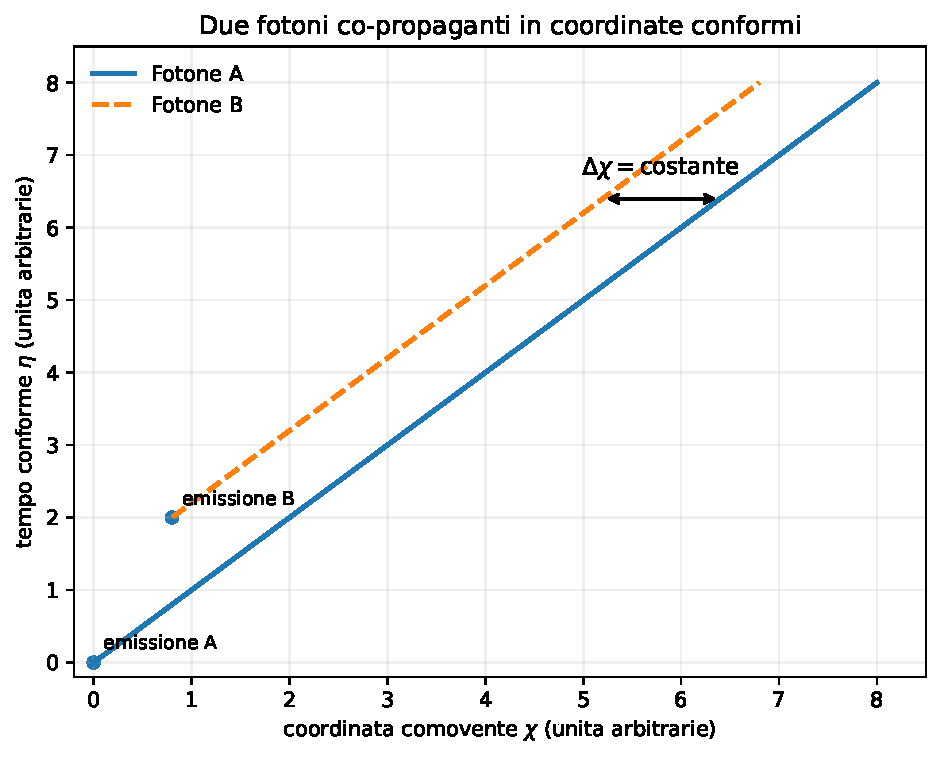
\includegraphics[width=0.76\textwidth]{conformal_two_photons.pdf}
\caption{Diagramma conforme schematico. Dopo l'emissione di $B$, i due raggi co-propaganti hanno la stessa pendenza nulla e una separazione comovente costante. La separazione propria e invece moltiplicata da $a(t)$.}
\label{fig:conformal}
\end{figure}

\subsection{Caso generale di due raggi radiali}

Introduciamo $s_i=\pm1$ per la direzione del raggio $i$:
\begin{equation}
 \dot\chi_i=s_i\frac{c}{a}.
\end{equation}
Per la separazione radiale firmata $D=a(\chi_1-\chi_2)$ si ottiene
\begin{equation}
 \boxed{\dot D=HD+(s_1-s_2)c.}
 \label{eq:master_two_rays}
\end{equation}
Questa equazione riassume il cuore cinematico dell'esplorazione:
\begin{itemize}
\item stessa direzione, $s_1=s_2$: $\dot D=HD$;
\item direzioni opposte, $s_1=+1$, $s_2=-1$: $\dot D=HD+2c$.
\end{itemize}
Il termine $2c$ e quindi reale come contributo causale per due fronti opposti, ma non rappresenta in generale l'intero tasso di crescita della loro distanza.

\textbf{Stato:} \status{DERIVATO ESATTAMENTE IN FLRW}.

\section{Tempo conforme e significato del termine $2c$}

Definiamo il tempo conforme
\begin{equation}
 d\eta=\frac{dt}{a(t)}.
\end{equation}
L'equazione nulla diventa
\begin{equation}
 \frac{d\chi}{d\eta}=\pm c.
\end{equation}
Per due raggi co-propaganti,
\begin{equation}
 \frac{d}{d\eta}(\chi_1-\chi_2)=c-c=0;
\end{equation}
per due raggi opposti,
\begin{equation}
 \frac{d}{d\eta}(\chi_1-\chi_2)=c-(-c)=2c.
\end{equation}
Il ``$c+c$'' cinematico appartiene dunque naturalmente alla separazione conforme di due fronti opposti, mentre nel problema originale dei due fotoni inseguitore/inseguito i due termini $c$ si cancellano.

\section{Orizzonti cosmologici e raggio di Hubble}

\subsection{Orizzonte delle particelle}

Il raggio proprio dell'orizzonte delle particelle e
\begin{equation}
 R_p(t)=a(t)\int_0^t\frac{c\,dt'}{a(t')}.
 \label{eq:particle_horizon}
\end{equation}
Derivando:
\begin{equation}
 \boxed{\dot R_p=HR_p+c.}
 \label{eq:particle_dot}
\end{equation}
Il diametro $2R_p$ soddisfa quindi
\begin{equation}
 \frac{d(2R_p)}{dt}=H(2R_p)+2c.
\end{equation}

\subsection{Orizzonte degli eventi}

Quando l'integrale converge,
\begin{equation}
 R_e(t)=a(t)\int_t^{\infty}\frac{c\,dt'}{a(t')},
\end{equation}
e
\begin{equation}
 \boxed{\dot R_e=HR_e-c.}
\end{equation}
Il segno opposto rispetto all'orizzonte delle particelle mostra che il termine $\pm c$ dipende dalla costruzione causale considerata.

\subsection{Raggio di Hubble}

Per
\begin{equation}
 R_H=\frac{c}{H}
\end{equation}
si ha
\begin{equation}
 \dot R_H=-c\frac{\dot H}{H^2}.
\end{equation}
Usando
\begin{equation}
 q=-1-\frac{\dot H}{H^2},
\end{equation}
otteniamo
\begin{equation}
 \boxed{\dot R_H=c(1+q).}
 \label{eq:hubble_radius_dot}
\end{equation}
Questo $2c$ ha origine dinamica diversa da quello di due raggi opposti.

\section{Perche $2c$ compare esattamente nell'era radiativa}

In un Universo dominato da radiazione,
\begin{equation}
 a(t)\propto t^{1/2},\qquad H=\frac{1}{2t},\qquad q=1.
\end{equation}
Dalla Eq.~\eqref{eq:hubble_radius_dot},
\begin{equation}
 \boxed{\dot R_H=2c.}
\end{equation}
Inoltre, dalla Eq.~\eqref{eq:particle_horizon},
\begin{equation}
 R_p=2ct,
\end{equation}
e quindi
\begin{equation}
 HR_p=c,
\end{equation}
cosicche
\begin{equation}
 \boxed{\dot R_p=HR_p+c=c+c=2c.}
\end{equation}

Questa coincidenza e speciale. Per una legge di potenza $a\propto t^n$ con $0<n<1$,
\begin{equation}
 R_H=\frac{ct}{n},\qquad R_p=\frac{ct}{1-n}.
\end{equation}
La condizione $R_H=R_p$ richiede $n=1/2$, cioe precisamente il caso radiativo.

\textbf{Stato:} \status{RISULTATO STANDARD, NON NUOVA LEGGE}.

\section{La variabile $\alpha=HR_p/c$}

Per mantenere l'intuizione causale senza imporre artificialmente $2c$ in ogni epoca, definiamo
\begin{equation}
 \boxed{\alpha(t)=\frac{H(t)R_p(t)}{c}.}
 \label{eq:alpha_def}
\end{equation}
La Eq.~\eqref{eq:particle_dot} diventa
\begin{equation}
 \boxed{\dot R_p=(1+\alpha)c.}
\end{equation}

\subsection{$\alpha$ costante}

Se $\alpha$ e costante, $R_p(0)=0$ implica
\begin{equation}
 R_p=(1+\alpha)ct.
\end{equation}
Dalla definizione di $\alpha$ segue
\begin{equation}
 H=\frac{\alpha}{(1+\alpha)t},
\end{equation}
e quindi
\begin{equation}
 \boxed{a(t)\propto t^{\alpha/(1+\alpha)}.}
 \label{eq:alpha_powerlaw}
\end{equation}
Ne risultano due casi notevoli:
\begin{equation}
 \alpha=1\Rightarrow a\propto t^{1/2}\quad(\text{radiazione}),
\end{equation}
\begin{equation}
 \alpha=2\Rightarrow a\propto t^{2/3}\quad(\text{materia}).
\end{equation}

\begin{figure}[ht]
\centering
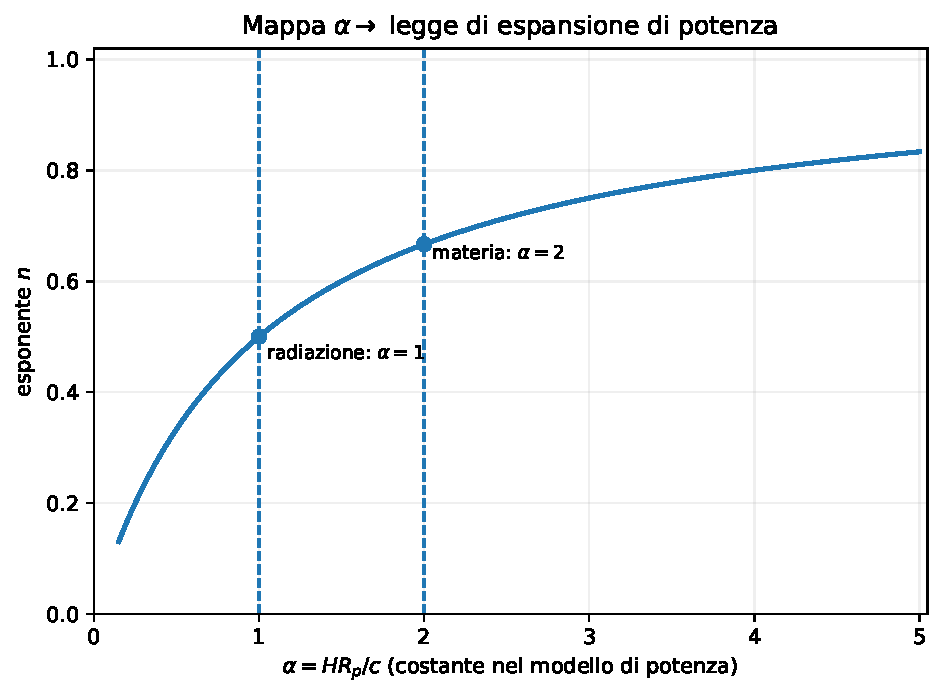
\includegraphics[width=0.72\textwidth]{alpha_powerlaw_map.pdf}
\caption{Per $\alpha$ costante, la legge di potenza ha esponente $n=\alpha/(1+\alpha)$. I valori $\alpha=1$ e $\alpha=2$ riproducono rispettivamente le leggi di potenza radiativa e materiale.}
\label{fig:alpha_map}
\end{figure}

Assumendo inoltre GR standard e un singolo fluido efficace con $p=w\rho c^2$, per $w>-1/3$ si ottiene
\begin{equation}
 \boxed{\alpha=\frac{2}{1+3w}.}
\end{equation}
Questa relazione e una riformulazione del comportamento di potenza, non una nuova equazione di stato.

\subsection{$\alpha$ variabile e parametro di decelerazione}

Derivando la Eq.~\eqref{eq:alpha_def} e usando Eq.~\eqref{eq:particle_dot} si ottiene
\begin{equation}
 \frac{d\alpha}{d\ln a}=1-\alpha q,
\end{equation}
cioe
\begin{equation}
 \boxed{q=\frac{1-d\alpha/d\ln a}{\alpha}.}
 \label{eq:q_alpha}
\end{equation}
Per avere $q<0$ con $\alpha>0$ e necessario
\begin{equation}
 \boxed{\frac{d\alpha}{d\ln a}>1.}
\end{equation}
La domanda dinamica diventa quindi: quale principio indipendente determina $\alpha(t)$?

\textbf{Stato:} \status{IDENTITA DERIVATA; CHIUSURA DINAMICA APERTA}.

\section{La variabile $\beta$ per i due fotoni}

Per due fotoni co-propaganti definiamo
\begin{equation}
 \beta(t)=\frac{H\Delta D}{c}.
\end{equation}
Poiche $\dot{\Delta D}=H\Delta D$,
\begin{equation}
 \dot{\Delta D}=\beta c.
\end{equation}
La separazione puo quindi crescere a $c$, $2c$ o a multipli maggiori senza che tali valori siano velocita locali di un fotone.

Dato che $\Delta D\propto a$,
\begin{equation}
 \boxed{\frac{d\ln\beta}{d\ln a}=-q.}
 \label{eq:beta_q}
\end{equation}
Dunque, durante una fase decelerante ($q>0$), $\beta$ diminuisce; durante una fase accelerante ($q<0$), $\beta$ aumenta.

Imporre $\beta=2$ costante non risolve il problema: dalla Eq.~\eqref{eq:beta_q} seguirebbe $q=0$, cioe nuovamente una cosmologia lineare. Inoltre $\beta$ dipende dalla coppia di fotoni scelta, quindi non e un candidato naturale a variabile cosmologica fondamentale.

\textbf{Stato:} \status{BUON DIAGNOSTICO, NON PRINCIPIO FONDAMENTALE IDENTIFICATO}.

\section{Collegamento con il redshift cosmologico}

La stessa struttura che mantiene costante la separazione comovente di due fotoni co-propaganti descrive la separazione tra creste successive di un'onda. Se $\Delta\chi$ e costante,
\begin{equation}
 \lambda_{\rm proper}(t)=a(t)\Delta\chi,
\end{equation}
per cui
\begin{equation}
 \frac{\lambda_{\rm obs}}{\lambda_{\rm em}}=\frac{a_{\rm obs}}{a_{\rm em}},
\end{equation}
e
\begin{equation}
 \boxed{1+z=\frac{a_{\rm obs}}{a_{\rm em}}.}
\end{equation}
L'intuizione che ``la distanza fra segnali luminosi cresce mentre entrambi viaggiano a $c$'' e quindi fisicamente reale ed e intimamente connessa al redshift cosmologico. Non richiede pero una velocita $c+c$ del singolo fotone.

\section{Controlli numerici illustrativi in un modello \LCDM}

Per verificare gli ordini di grandezza e stata usata una realizzazione piatta illustrativa con
\begin{equation}
 H_0=67.4\ \mathrm{km\,s^{-1}\,Mpc^{-1}},\qquad \Omega_m=0.315,
\end{equation}
\begin{equation}
 \Omega_r=9.2\times10^{-5},\qquad \Omega_\Lambda=1-\Omega_m-\Omega_r.
\end{equation}
I primi due valori sono coerenti con i parametri base di Planck 2018 \cite{Planck2018}. $\Omega_r$ qui e usato come valore illustrativo sufficiente ai controlli; non e un fit dedicato.

Come proxy fisicamente definito per un raggio libero molto antico e stato scelto $t_A=0.38$ Myr, circa l'epoca del disaccoppiamento. Non si assume che esista un ``primo fotone'' unico del Big Bang: prima della ricombinazione l'Universo era un plasma opaco alla propagazione libera dei fotoni CMB.

\subsection{Stessa origine comovente, emissione ritardata di B}

Se $A$ parte a $t_A$ e $B$ dalla stessa origine a $t_B>t_A$, la separazione propria odierna e
\begin{equation}
 \Delta D_0=c\int_{t_A}^{t_B}\frac{dt}{a(t)},
\end{equation}
e il tasso odierno vale $H_0\Delta D_0$. I risultati numerici sono:

\begin{table}[ht]
\centering
\caption{Controllo numerico per due fotoni co-propaganti emessi dalla stessa origine. Le velocita indicate sono tassi di crescita della separazione propria, non velocita locali dei fotoni.}
\begin{tabular}{rcc}
\toprule
$t_B$ dopo il Big Bang & $\Delta D_0$ [Gly] & $H_0\Delta D_0/c$ \\
\midrule
1 Myr   & 0.483 & 0.033 \\
10 Myr  & 2.662 & 0.184 \\
100 Myr & 7.562 & 0.521 \\
1 Gyr   & 18.243 & 1.258 \\
5 Gyr   & 32.342 & 2.229 \\
\bottomrule
\end{tabular}
\label{tab:numeric_same_origin}
\end{table}

La condizione $H_0\Delta D_0=2c$ corrisponde, in questo modello e con $t_A=0.38$ Myr, a
\begin{equation}
 \Delta D_0=\frac{2c}{H_0}\simeq29.015\ \Gly,
\end{equation}
che si ottiene per
\begin{equation}
 \boxed{t_B\simeq3.660\ \Gyr.}
\end{equation}
Il valore $2c$ non e quindi privilegiato: e semplicemente una soglia geometrica $\Delta D=2c/H$.

\subsection{B emesso da una sorgente gia lontana}

In un secondo esempio, $B$ e emesso a $t_B=10$ Gyr da una sorgente a coordinata comovente $\chi_s=10$ Gly. Nel modello sopra si trova $a(t_B)\simeq0.754$. Al momento dell'emissione di $B$:
\begin{align}
D_A&\simeq30.783\ \Gly,\\
D_B&\simeq7.536\ \Gly,\\
\Delta D&\simeq23.247\ \Gly,\\
\dot{\Delta D}/c&\simeq1.910.
\end{align}
Oggi:
\begin{align}
D_A&\simeq45.210\ \Gly,\\
D_B&\simeq14.363\ \Gly,\\
\Delta D&\simeq30.847\ \Gly,\\
\dot{\Delta D}/c&\simeq2.126.
\end{align}
Ancora una volta entrambi i fotoni hanno velocita locale $c$; il valore $>2c$ riguarda la crescita della separazione propria.

Nello stesso esempio il raggio di Hubble odierno e circa $14.507$ Gly e l'orizzonte degli eventi e circa $16.679$ Gly. Il fotone $B$, diretto verso l'esterno, attraverserebbe il raggio di Hubble dopo circa $0.095$ Gyr e l'orizzonte degli eventi dell'osservatore dopo circa $1.206$ Gyr, se il modello \LCDM\ illustrativo fosse estrapolato nel futuro. Questi valori sono esempi model-dependent e non elementi fondamentali dell'ipotesi.

\section{Perche la relazione $\dot D=HD\pm c$ non chiude la dinamica}

La Eq.~\eqref{eq:master_two_rays} e una conseguenza della metrica FLRW una volta assegnato $a(t)$. Essa determina la traiettoria o la separazione di segnali luminosi dato $H(t)$, ma non determina $H(t)$ stesso. In altre parole,
\begin{equation}
 \boxed{\dot D=HD\pm c\quad\text{e cinematica, non una equazione dinamica chiusa}.}
\end{equation}
Per ottenere l'evoluzione di $a(t)$ serve un principio ulteriore. Nella cosmologia standard tale ruolo e svolto dalle equazioni di Einstein/Friedmann e dal contenuto di energia-impulso.

Questo e il principale ``gate'' concettuale raggiunto finora: qualunque teoria nuova deve fornire una chiusura indipendente, non scegliere una funzione $\alpha(t)$ o $H(t)$ costruita per riprodurre a posteriori i dati.

\section{Ramo successivo: causalita, orizzonte apparente e termodinamica}

Esiste un precedente teorico importante: applicando una relazione termodinamica al cosiddetto orizzonte apparente di un Universo FRW, insieme a un'entropia proporzionale all'area, e possibile derivare le equazioni di Friedmann \cite{CaiKim2005}. Questo non dimostra la nostra ipotesi e non identifica l'orizzonte delle particelle con l'orizzonte apparente. Mostra pero che un legame tra dinamica cosmologica, proprieta degli orizzonti e termodinamica e una strada fisicamente seria.

Per un FLRW con curvatura spaziale $k$, il raggio dell'orizzonte apparente e
\begin{equation}
 R_A=\frac{c}{\sqrt{H^2+kc^2/a^2}}.
\end{equation}
Nel caso piatto $k=0$ coincide con $R_H=c/H$, ma non coincide in generale con l'orizzonte delle particelle $R_p$.

Il prossimo obiettivo e quindi confrontare quantitativamente
\begin{equation}
 R_p,\qquad R_H,\qquad R_A,\qquad R_e,
\end{equation}
e verificare se una condizione basata su conservazione, flusso di energia, entropia o informazione possa determinare $\alpha(t)$ senza inserire la storia dell'espansione a mano.


\section{Gate R8: confronto tra orizzonti e chiusura termodinamica}

\subsection{Quattro scale, tre oggetti distinti nel caso piatto}

Per una metrica FLRW con curvatura spaziale $k$, il raggio dell'orizzonte apparente e
\begin{equation}
 R_A=\frac{c}{\sqrt{H^2+kc^2/a^2}}.
 \label{eq:apparent_horizon}
\end{equation}
Nel caso spazialmente piatto,
\begin{equation}
 \boxed{R_A=R_H=\frac{c}{H}.}
\end{equation}
Quindi il nostro parametro causale diventa direttamente un rapporto tra orizzonti:
\begin{equation}
 \boxed{\alpha=\frac{HR_p}{c}=\frac{R_p}{R_A}}\qquad(k=0).
 \label{eq:alpha_ratio}
\end{equation}
Per l'orizzonte degli eventi definiamo analogamente
\begin{equation}
 \boxed{\varepsilon=\frac{HR_e}{c}=\frac{R_e}{R_A}}\qquad(k=0).
 \label{eq:epsilon_def}
\end{equation}
Usando $\dot R_p=HR_p+c$, $\dot R_e=HR_e-c$ e $q=-1-\dot H/H^2$ si ottengono le due equazioni esatte
\begin{align}
 \boxed{\frac{d\alpha}{d\ln a}=1-q\alpha},\label{eq:alpha_evol_r8}\\
 \boxed{\frac{d\varepsilon}{d\ln a}=-1-q\varepsilon}.\label{eq:epsilon_evol_r8}
\end{align}
Esse hanno una struttura speculare: il particle horizon integra il passato causale e porta un termine $+1$, mentre l'event horizon integra il futuro e porta un termine $-1$.

\subsection{La termodinamica dell'orizzonte apparente recupera Friedmann}

In questa sottosezione poniamo $c=\hbar=k_B=1$ per rendere trasparente la struttura. All'orizzonte apparente si assegnano, in GR di Einstein,
\begin{equation}
 S_A=\frac{A_A}{4G},\qquad T_A\simeq\frac{1}{2\pi R_A},
\end{equation}
con $A_A=4\pi R_A^2$. Per un fluido perfetto, il flusso energetico attraverso l'orizzonte e proporzionale a
\begin{equation}
 \delta Q=A_A(\rho+p)HR_A\,dt.
\end{equation}
La relazione di Clausius $\delta Q=T_A dS_A$ conduce a
\begin{equation}
 \boxed{\dot H-\frac{k}{a^2}=-4\pi G(\rho+p)},
 \label{eq:thermo_raychaudhuri}
\end{equation}
mentre, combinata con la conservazione
\begin{equation}
 \dot\rho+3H(\rho+p)=0,
\end{equation}
restituisce
\begin{equation}
 \boxed{H^2+\frac{k}{a^2}=\frac{8\pi G}{3}\rho+\mathrm{costante}.}
 \label{eq:thermo_friedmann}
\end{equation}
Questa equivalenza e il risultato classico di Cai e Kim e del formalismo della unified first law sull'orizzonte apparente \cite{CaiKim2005,CaiCao2007}.

Il punto decisivo per il nostro progetto e pero negativo: Eqs.~\eqref{eq:thermo_raychaudhuri}--\eqref{eq:thermo_friedmann} non scelgono da sole $p(\rho)$. Senza un'equazione di stato o una dinamica addizionale del contenuto cosmico, $H(t)$ non e univocamente determinato. Di conseguenza la termodinamica standard dell'orizzonte apparente \emph{non chiude} autonomamente $\alpha(t)$.

\subsection{Perche non trasferire semplicemente la stessa termodinamica a $R_p$}

L'orizzonte apparente e una superficie locale di trapping; il particle horizon e invece una quantita globale che dipende dall'intera storia passata. Con le assegnazioni piu semplici $S\propto A$ e $T\propto1/R$, la prima legge non e genericamente soddisfatta sul particle horizon in Einstein gravity, mentre lo e sull'apparente \cite{BhattacharyaDebnath2011}. Per l'event horizon esistono costruzioni che recuperano una prima legge ridefinendone opportunamente la temperatura \cite{TuChen2016}; questo mostra pero che la scelta termodinamica aggiunge struttura, non la deriva dalla sola causalita.

Pertanto assegnare direttamente a $R_p$ una entropia Bekenstein--Hawking e usarla come nuova equazione dinamica sarebbe, allo stato attuale, un'ipotesi aggiuntiva e non una conseguenza del nostro punto di partenza.

\subsection{Seconda legge: vincolo, non chiusura}

Nel caso piatto $R_A=c/H$ e l'entropia geometrica standard soddisfa $S_A\propto H^{-2}$. Ne segue
\begin{equation}
 \boxed{\frac{d\ln S_A}{d\ln a}=2(1+q).}
 \label{eq:entropy_q}
\end{equation}
Se si considera il solo contributo geometrico e si richiede $\dot S_A\ge0$ durante espansione, si ottiene semplicemente
\begin{equation}
 q\ge-1.
\end{equation}
La saturazione $\dot S_A=0$ seleziona $q=-1$, cioe de Sitter. Si tratta pero di una disuguaglianza o di una condizione di equilibrio, non di una legge che ricostruisca la transizione radiazione $\rightarrow$ materia $\rightarrow$ accelerazione. In analisi termodinamiche complete deve inoltre essere incluso anche il contributo entropico della materia.

\subsection{Test informazionale: il precedente dell'energia oscura olografica}

Un controllo indipendente viene dai modelli di holographic dark energy, nei quali una densita efficace viene legata a una scala IR $L$ tramite $\rho_{\rm de}\propto L^{-2}$. Nella formulazione standard, scegliere $L=H^{-1}$ o il particle horizon non produce l'accelerazione tardiva; la scelta del future event horizon puo invece farlo \cite{Akhlaghi2018}. Modifiche recenti dell'entropia possono cambiare questa conclusione anche mantenendo il particle horizon, ma introducono esplicitamente nuova fisica oltre a GR e all'entropia area standard \cite{Asvar2026}.

Questo risultato e importante per la nostra roadmap: il solo passato causale $R_p$, combinato con la prescrizione olografica standard, non genera gratuitamente la fase accelerata osservata.

\subsection{Gate R8: esito}

\begin{center}
\boxed{\text{APPARENT-HORIZON THERMODYNAMICS: PASS; }\alpha\text{-CLOSURE: NOT DERIVED}}
\end{center}

La termodinamica dell'orizzonte apparente ha quindi un contenuto dinamico reale e ricostruisce GR/Friedmann, ma non determina da sola quale fluido o quale equazione di stato governi l'Universo. Il nostro problema si sposta: una nuova teoria dovrebbe motivare una legge per il contenuto energetico, per l'entropia dell'orizzonte o per il flusso che sia indipendente dai dati da spiegare.

\section{Gate R9: dinamica congiunta di passato e futuro causale}

\subsection{Forma conforme}

Nel caso piatto, scegliendo $\eta=0$ al Big Bang,
\begin{equation}
 R_p=a c\eta.
\end{equation}
Se il futuro conforme totale e finito, $\eta_\infty<\infty$, allora
\begin{equation}
 R_e=a c(\eta_\infty-\eta).
\end{equation}
Con la Hubble conforme $\mathcal H=aH$ si possono scrivere, in unita $c=1$,
\begin{equation}
 \boxed{\alpha=\mathcal H\eta,\qquad \varepsilon=\mathcal H(\eta_\infty-\eta).}
 \label{eq:conformal_alpha_epsilon}
\end{equation}
Questa forma mostra che $\alpha$ misura quanta storia causale passata e contenuta in un raggio apparente, mentre $\varepsilon$ confronta la scala locale con il futuro causalmente accessibile.

\subsection{Interpolazione esatta radiazione--materia}

Per un Universo piatto contenente soltanto radiazione e materia, la soluzione in tempo conforme puo essere scritta
\begin{equation}
 a(\eta)=A\eta+B\eta^2,
\end{equation}
con $A,B>0$. Definendo $y=B\eta/A$,
\begin{equation}
 \boxed{\alpha=\frac{1+2y}{1+y}}.
 \label{eq:alpha_radmatter_exact}
\end{equation}
Pertanto
\begin{equation}
 \alpha\to1\quad(\text{radiazione}),\qquad \alpha\to2\quad(\text{materia}).
\end{equation}
La transizione $1\rightarrow2$ non deve essere inserita a mano: segue esattamente dalla miscela radiazione--materia una volta assunte le equazioni standard di Friedmann.

\begin{figure}[ht]
\centering
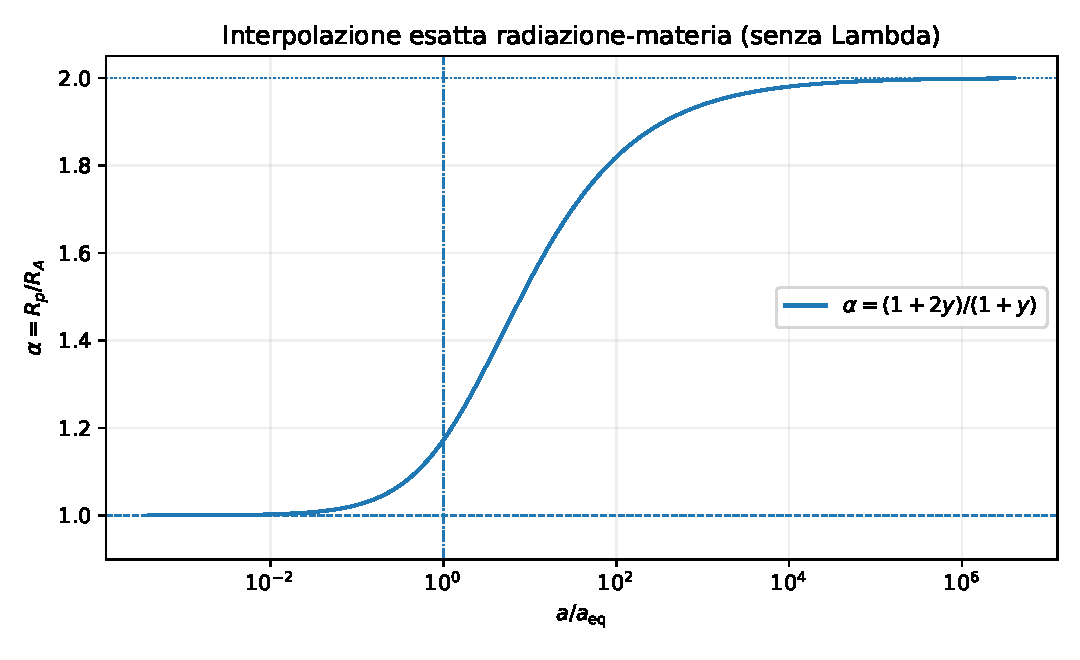
\includegraphics[width=0.73\textwidth]{alpha_radiation_matter_exact.pdf}
\caption{Interpolazione analitica di $\alpha=R_p/R_A$ in un Universo piatto con radiazione e materia, senza costante cosmologica. La variabile passa da $1$ a $2$ senza un ansatz ad hoc.}
\label{fig:alpha_radmatter_exact}
\end{figure}

\subsection{Aggiunta di una fase accelerata}

In un modello piatto illustrativo $\Lambda$CDM, l'accelerazione tardiva fa crescere $\alpha$ oltre il valore materiale, mentre $\varepsilon$ tende verso l'unita nel limite de Sitter. Con i parametri numerici gia usati nel documento si ottiene oggi, approssimativamente,
\begin{equation}
 q_0\simeq-0.527,\qquad \alpha_0\simeq3.18,\qquad \varepsilon_0\simeq1.15,
\end{equation}
cioe
\begin{equation}
 R_p\simeq46.1\ \Gly,\qquad R_A\simeq14.5\ \Gly,\qquad R_e\simeq16.7\ \Gly.
\end{equation}
L'inizio dell'accelerazione ($q=0$) avviene, in questa realizzazione illustrativa, a $z\simeq0.63$ con $\alpha\simeq2.32$.

\begin{figure}[ht]
\centering
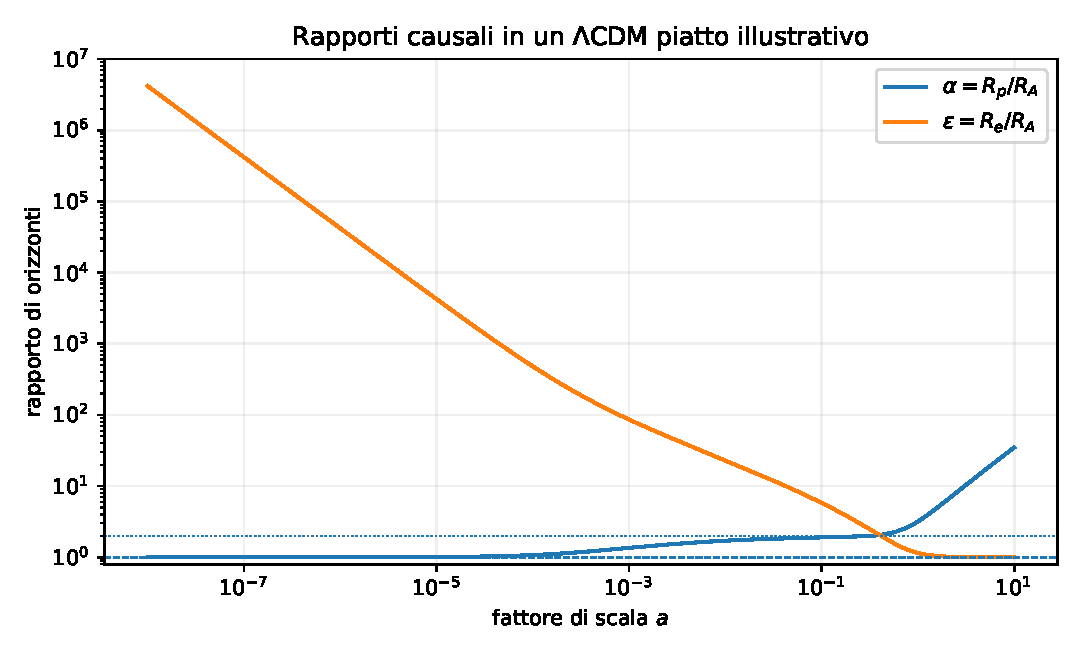
\includegraphics[width=0.75\textwidth]{horizon_ratios_lcdm.pdf}
\caption{Evoluzione illustrativa dei rapporti $\alpha=R_p/R_A$ ed $\varepsilon=R_e/R_A$ in un modello piatto $\Lambda$CDM. Il particle horizon conserva memoria integrata del passato e il suo rapporto con $R_A$ cresce fortemente nella fase accelerata; l'event horizon tende invece a coincidere con $R_A$ nel limite de Sitter.}
\label{fig:horizon_ratios}
\end{figure}

\subsection{Interpretazione del Gate R9}

Questi risultati rafforzano una conclusione metodologica: $\alpha$ e $\varepsilon$ sono eccellenti variabili diagnostiche della struttura causale, ma non sono variabili dinamiche indipendenti. Una volta specificato $H(a)$, entrambe sono determinate da integrali causali. Invertire il ragionamento e usare una legge per $\alpha$ come fondamento e possibile solo se quella legge nasce da un principio indipendente e produce predizioni ulteriori.

Il prossimo gate utile non e quindi cercare un'altra coincidenza numerica con $2c$, ma testare classi minime di chiusura: (i) una legge entropica modificata $S(A)$, (ii) una relazione flusso--informazione sull'orizzonte apparente, oppure (iii) una dinamica del contenuto energetico derivata da un principio causale. Ogni ramo dovra recuperare radiazione e materia senza fit ad hoc e produrre autonomamente una fase accelerata falsificabile.


\section{Gate R10: mappa entropia--Friedmann e prime chiusure candidate}
\label{sec:r10_entropy}

Questo gate non assume che una nuova legge entropica sia vera. Lo scopo e piu modesto e falsificabile: derivare una mappa generale che dica quale dinamica di background segue da una assegnazione $S(A)$ all'orizzonte apparente, quindi sottoporre a test alcune famiglie motivate indipendentemente. In questa sezione si usano unita naturali $c=\hbar=k_B=1$; i fattori di $c$ possono essere ripristinati dimensionalmente.

Definiamo
\begin{equation}
 X\equiv H^2+\frac{k}{a^2}=R_A^{-2},\qquad A=4\pi R_A^2=\frac{4\pi}{X},
\end{equation}
e indichiamo con
\begin{equation}
 S_A\equiv\frac{dS}{dA}
\end{equation}
la derivata della generica entropia di orizzonte. Con temperatura di Hawking $T=(2\pi R_A)^{-1}$ e flusso di calore
\begin{equation}
 \delta Q=A(\rho+p)H R_A\,dt,
\end{equation}
la relazione di Clausius $\delta Q=T\,dS$ conduce a
\begin{equation}
 \boxed{\dot H-\frac{k}{a^2}=-\frac{\pi(\rho+p)}{S_A}.}
 \label{eq:generic_entropy_raychaudhuri}
\end{equation}
Usando la conservazione standard
\begin{equation}
 \dot\rho+3H(\rho+p)=0
\end{equation}
si ottiene la mappa entropia--Friedmann
\begin{equation}
 \boxed{\frac{d\rho}{dX}=\frac{3}{2\pi}\,S_A\!\left(\frac{4\pi}{X}\right),}
 \label{eq:entropy_friedmann_map}
\end{equation}
ossia
\begin{equation}
 \boxed{\rho(X)=C+\frac{3}{2\pi}\int^X S_A\!\left(\frac{4\pi}{\xi}\right)d\xi.}
 \label{eq:entropy_friedmann_integral}
\end{equation}
Per $S=A/(4G)$ si recupera
\begin{equation}
 \rho=C+\frac{3X}{8\pi G},
\end{equation}
e l'integrazione libera equivale a una costante cosmologica. Questo punto e importante: anche la termodinamica standard non predice il valore di $\Lambda$; lo lascia come costante di integrazione. La struttura generale e coerente con il programma gravita--termodinamica di Jacobson e Cai--Kim \cite{Jacobson1995,CaiKim2005}.

\subsection{Test A: entropia di potenza costante}

Prendiamo
\begin{equation}
 S(A)=\sigma A^\nu,
\end{equation}
con $\nu$ costante e $\nu\neq2$. Dalla Eq.~\eqref{eq:entropy_friedmann_map} segue
\begin{equation}
 \rho-C=\frac{3\sigma\nu(4\pi)^{\nu-1}}{2\pi(2-\nu)}X^{2-\nu}.
 \label{eq:power_entropy_friedmann}
\end{equation}
Nel caso piatto, $C=0$ e fluido barotropico $p=w\rho$, la conservazione da $\rho\propto a^{-3(1+w)}$ e quindi
\begin{equation}
 a(t)\propto t^m,\qquad
 m=\frac{2(2-\nu)}{3(1+w)},
\end{equation}
con
\begin{equation}
 \boxed{q=\frac{3(1+w)}{2(2-\nu)}-1.}
 \label{eq:q_power_entropy}
\end{equation}
Riprodurre sia $a\propto t^{1/2}$ durante la radiazione sia $a\propto t^{2/3}$ durante la materia impone in entrambi i casi $\nu=1$, cioe la legge di Bekenstein--Hawking. Con sola materia non relativistica, l'accelerazione richiede invece $\nu<1/2$. Una singola potenza costante non puo quindi essere contemporaneamente quasi standard nelle ere precoci e diventare da sola il motore dell'accelerazione tardiva.

La Barrow entropy $S\propto A^{1+\Delta/2}$ ha $0\leq\Delta\leq1$ \cite{Saridakis2020}; nel sottoramo volutamente minimale $C=0$ e singolo fluido ordinario essa non produce accelerazione da polvere. Questo non contraddice i modelli Barrow completi pubblicati, che mantengono ulteriori termini/integrali e possono essere riscritti come un settore di energia oscura efficace \cite{Saridakis2020}. Il nostro test isola soltanto cio che fa l'esponente costante da solo.

\begin{figure}[ht]
\centering
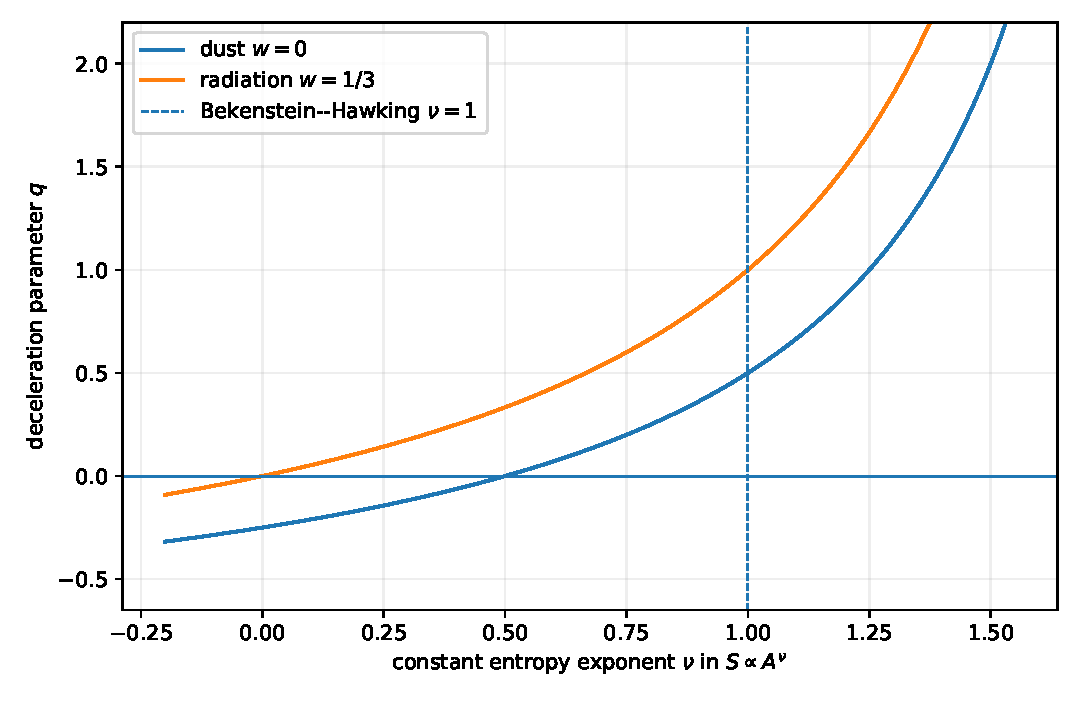
\includegraphics[width=0.76\textwidth]{entropy_powerlaw_q.pdf}
\caption{Parametro di decelerazione nella chiusura minimale $S\propto A^\nu$, $C=0$, per radiazione e materia. La legge standard e $\nu=1$; una potenza costante che preserva le ere standard non genera poi autonomamente l'accelerazione tardiva.}
\label{fig:entropy_powerlaw_q}
\end{figure}

\subsection{Test B: correzione logaritmica dell'area}

Consideriamo la correzione quantistica schematica
\begin{equation}
 S(A)=\frac{A}{4G}+\gamma\ln\!\left(\frac{A}{A_*}\right).
\end{equation}
La mappa generale fornisce
\begin{equation}
 \boxed{\rho-C=\frac{3X}{8\pi G}+\frac{3\gamma X^2}{16\pi^2}.}
 \label{eq:log_entropy_friedmann}
\end{equation}
Il termine nuovo scala come $X^2\sim H^4$ e quindi e relativamente piu importante ad alta curvatura. A bassa curvatura il termine lineare standard domina. Nel ramo minimale senza una costante cosmologica separata, questa correzione non fornisce dunque un meccanismo naturale per accendere l'accelerazione soltanto tardi. Correzioni logaritmiche dell'entropia e Friedmann modificate di questo tipo sono note in letteratura \cite{CaiCaoHu2008}.

\textbf{Esito Test B:} \status{FALLITO COME MOTORE IR MINIMALE}; resta eventualmente rilevante per dinamica ad alta curvatura.

\subsection{Test C: una forma tipo Renyi come controllo IR}

Per verificare che la mappa sia capace anche di produrre modifiche infrarosse, consideriamo
\begin{equation}
 S_R(A)=\frac{1}{\lambda}\ln\!\left(1+\lambda\frac{A}{4G}\right),\qquad \lambda>0,
 \label{eq:renyi_entropy}
\end{equation}
una forma di tipo Renyi gia esplorata in cosmologia di orizzonte \cite{Fazlollahi2022}. Definiamo
\begin{equation}
 b\equiv\frac{\pi\lambda}{G}.
\end{equation}
Allora
\begin{equation}
 S_A=\frac{X}{4G(X+b)}
\end{equation}
e la Eq.~\eqref{eq:entropy_friedmann_integral}, scegliendo la costante additiva in modo che il termine fra parentesi si annulli per $X\to0$, produce
\begin{equation}
 \boxed{\rho-C=\frac{3}{8\pi G}\left[X-b\ln\!\left(1+\frac{X}{b}\right)\right].}
 \label{eq:renyi_friedmann}
\end{equation}
Per $X\gg b$ il termine dominante e quello standard, mentre per $X\ll b$
\begin{equation}
 \rho-C\simeq\frac{3X^2}{16\pi G b}.
\end{equation}
Con polvere e $C=0$ cio implica asintoticamente
\begin{equation}
 H^2\propto\rho^{1/2},\qquad a(t)\propto t^{4/3},\qquad q\to-\frac14.
\end{equation}
Definendo $y=X/b$, il parametro di decelerazione del ramo di polvere e
\begin{equation}
 \boxed{q(y)=-1+\frac32\frac{(1+y)[y-\ln(1+y)]}{y^2}.}
 \label{eq:renyi_q}
\end{equation}
Esso tende a $1/2$ per $y\gg1$, attraversa $q=0$ a $y\simeq1.81696$ e tende a $-1/4$ per $y\ll1$.

\begin{figure}[ht]
\centering
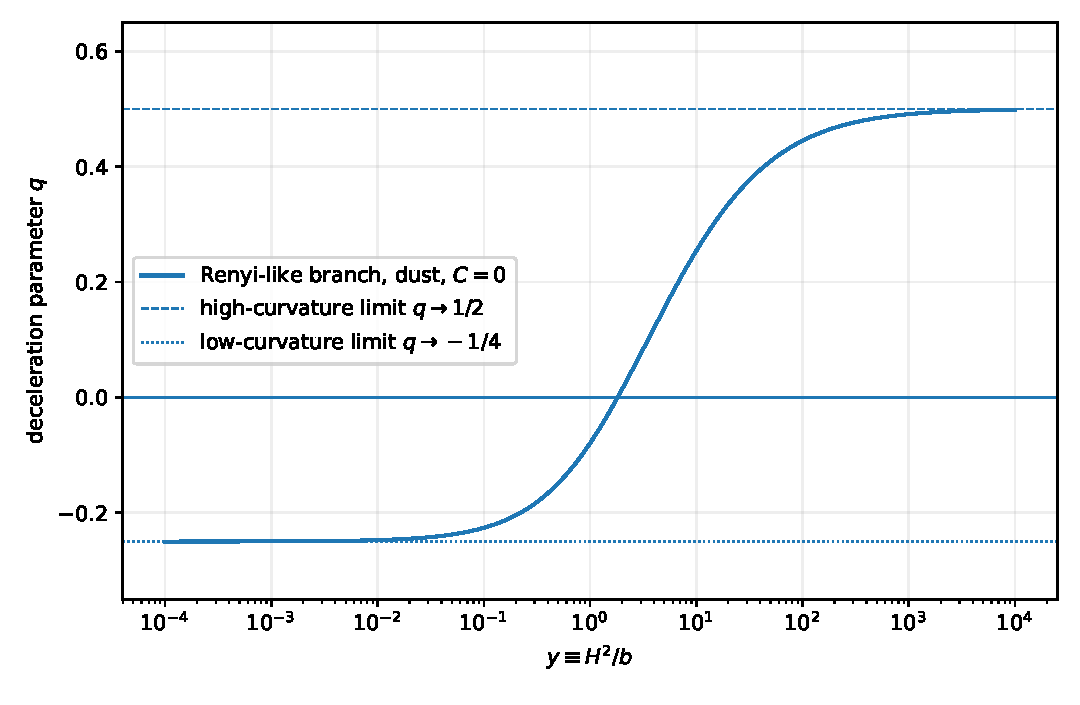
\includegraphics[width=0.76\textwidth]{renyi_minimal_q.pdf}
\caption{Chiusura tipo Renyi nel ramo minimale con polvere e $C=0$. L'alta curvatura recupera il comportamento materiale standard, mentre a bassa curvatura emerge una accelerazione di potenza con $q\to-1/4$.}
\label{fig:renyi_minimal_q}
\end{figure}

Questo test e metodologicamente utile perche mostra che una singola deformazione entropica puo in principio produrre una transizione senza prescrivere a mano una funzione $\alpha(a)$. Tuttavia non costituisce un risultato originale del progetto: la Renyi horizon cosmology appartiene a una letteratura preesistente. Inoltre il limite $q\to-1/4$ non e de Sitter e la compatibilita quantitativa con i dati deve essere verificata, non assunta.

\textbf{Esito Test C:} \status{SURVIVES AS CONTROL TOY MODEL / NON ORIGINALE}.

\subsection{Verdetto del Gate R10}

La Eq.~\eqref{eq:entropy_friedmann_map} e il risultato generale utile del gate. Essa dimostra anche il limite concettuale della strategia: scegliere $S(A)$ equivale a introdurre nuova fisica gravitazionale. Come sottolineato esplicitamente nella letteratura sulla Barrow cosmology, se la relazione entropica modificata deve essere nota a priori, la procedura termodinamica non crea da sola la teoria sottostante \cite{Saridakis2020}.

Per il progetto $c+c$ il verdetto e quindi:
\begin{enumerate}
\item la chiusura $S(A)$ e tecnicamente capace di generare Friedmann modificate;
\item una potenza costante e una correzione logaritmica non realizzano la sequenza desiderata nel ramo minimale;
\item una deformazione IR tipo Renyi puo generare una transizione, ma e un'ipotesi esterna gia nota e non e stata derivata dalla causalita o dai due fotoni;
\item non e ancora stata derivata alcuna $S(A)$ specifica dall'intuizione $c+c$.
\end{enumerate}

\textbf{Gate R10:} \status{GENERIC MAP PASS; CAUSAL ENTROPY CLOSURE NOT DERIVED}.


\section{Gate R11: flusso energia--informazione e ridondanza delle chiusure note}
\label{sec:r11_info}

Il Gate R10 ha mostrato che assumere una funzione $S(A)$ produce una dinamica gravitazionale modificata, ma non spiega perche quella funzione debba essere scelta. Il Gate R11 chiede quindi se un principio informazionale piu elementare possa aggiungere una equazione indipendente. Sono stati testati tre candidati noti, senza adattarne i parametri alla storia cosmologica desiderata.

\subsection{Test A: Landauer a saturazione}

Il principio di Landauer associa alla cancellazione irreversibile di un bit un costo energetico minimo $E_{\rm bit}=k_B T\ln2$ \cite{Landauer1961}. Se l'entropia di orizzonte $S$ viene espressa come numero di bit
\begin{equation}
 N=\frac{S}{k_B\ln2},
\end{equation}
allora, nel limite di saturazione di Landauer,
\begin{equation}
 \dot E_{\rm L}=k_B T\ln2\,\dot N=T\dot S.
\end{equation}
Ma la relazione termodinamica usata nei Gate R8--R10 e precisamente
\begin{equation}
 \dot Q=T\dot S.
\end{equation}
Pertanto identificare il flusso energetico di orizzonte con un flusso informazionale Landauer al limite minimo non fornisce una seconda equazione:
\begin{equation}
 \boxed{\dot E_{\rm L}=\dot Q\quad\Longleftrightarrow\quad \text{Clausius gia imposto}.}
\end{equation}
Se Landauer non e saturato, resta una disuguaglianza e non una chiusura dinamica univoca.

\textbf{Esito Test A:} \status{RIDONDANTE / NESSUNA NUOVA CHIUSURA}.

\subsection{Test B: saturazione del bound di Bekenstein}

Il bound di Bekenstein per un sistema di energia $E$ e raggio efficace $R$ e, in unita naturali,
\begin{equation}
 S\leq2\pi E R
\end{equation}
\cite{Bekenstein1981}. Come controllo estremo, poniamo $R=R_A$, $E=\rho V$ con $V=4\pi R_A^3/3$, e imponiamo simultaneamente la saturazione del bound e l'uguaglianza con l'entropia di orizzonte $S_A=\pi R_A^2/G$. Si ottiene
\begin{equation}
 \frac{\pi R_A^2}{G}=2\pi\left(\rho\frac{4\pi R_A^3}{3}\right)R_A,
\end{equation}
cioe
\begin{equation}
 \boxed{\rho=\frac{3}{8\pi G R_A^2}.}
\end{equation}
Nel caso piatto $R_A=H^{-1}$ questa e esattamente
\begin{equation}
 \boxed{H^2=\frac{8\pi G}{3}\rho.}
\end{equation}
Il risultato e istruttivo ma non chiude la cosmologia: non determina $p(\rho)$, non genera la successione radiazione--materia--accelerazione e richiede una saturazione che non e genericamente valida per il contenuto cosmologico ordinario. Inoltre il bound originale e stato formulato per sistemi limitati con ipotesi che non possono essere trasferite senza cautela a una regione cosmologica fortemente gravitante.

\textbf{Esito Test B:} \status{RICOSTRUISCE FRIEDMANN SOTTO SATURAZIONE FORTE; NON CHIUDE}.

\subsection{Test C: holographic equipartition}

Padmanabhan ha proposto che l'espansione dello spazio cosmico possa essere espressa mediante una differenza fra gradi di liberta di superficie e di volume \cite{Padmanabhan2012}. Nel caso piatto, con raggio di Hubble $R_H=H^{-1}$,
\begin{equation}
 V=\frac{4\pi}{3H^3},\qquad N_{\rm sur}=\frac{4\pi}{G H^2},\qquad T=\frac{H}{2\pi}.
\end{equation}
Usando per il bulk l'energia gravitazionale attiva $E=(\rho+3p)V$ e la regola di equipartizione, con il segno convenzionale appropriato al ramo accelerato,
\begin{equation}
 N_{\rm bulk}=-\frac{2(\rho+3p)V}{T},
\end{equation}
la legge
\begin{equation}
 \frac{dV}{dt}=G(N_{\rm sur}-N_{\rm bulk})
\end{equation}
porta direttamente a
\begin{equation}
 \boxed{\dot H+H^2=-\frac{4\pi G}{3}(\rho+3p),}
\end{equation}
cioe l'equazione standard di accelerazione. Con la continuita si recupera la Friedmann fino a una costante d'integrazione.

Il punto decisivo per il nostro progetto e che $N_{\rm bulk}$ contiene gia $\rho+3p$: l'informazione che distingue radiazione, materia e componente accelerante viene importata dal contenuto energetico, non ricavata dalla causalita del bordo.

\textbf{Esito Test C:} \status{PASS COME RIFORMULAZIONE DI GR; FAIL COME CHIUSURA AUTONOMA}.

\subsection{Un controllo direttamente legato a $R_p/R_A$}

Nel caso piatto, se si assegna formalmente un'entropia di area sia a $R_A$ sia al particle horizon,
\begin{equation}
 \frac{S_p}{S_A}=\frac{R_p^2}{R_A^2}=\alpha^2.
\end{equation}
Le rispettive velocita logaritmiche sono
\begin{align}
 \frac{1}{H}\frac{\dot S_A}{S_A}&=2(1+q),\\
 \frac{1}{H}\frac{\dot S_p}{S_p}&=2\left(1+\frac1\alpha\right).
\end{align}
Imporre l'uguaglianza dei due tassi relativi conduce a
\begin{equation}
 q=\frac1\alpha,
\end{equation}
ma, usando $\alpha'=1-q\alpha$, equivale semplicemente a
\begin{equation}
 \boxed{\alpha'=0.}
\end{equation}
La presunta ``legge informazionale'' non e quindi una nuova dinamica: afferma soltanto che il rapporto $R_p/R_A$ resta costante. Descrive bene i punti fissi di pure ere di potenza, per esempio $\alpha=1$ nella radiazione e $\alpha=2$ nella materia, ma non spiega la transizione fra esse ne l'accelerazione tardiva.

\subsection{Verdetto del Gate R11}

I tre principi informazionali esaminati convergono sullo stesso limite:
\begin{enumerate}
\item Landauer a saturazione e algebraicamente equivalente a Clausius;
\item Bekenstein a saturazione estrema ricostruisce la prima Friedmann ma non l'equazione di stato;
\item holographic equipartition ricostruisce l'equazione di accelerazione introducendo esplicitamente $\rho+3p$.
\end{enumerate}
Nessuno produce una legge autonoma per $\alpha(t)$ o $H(t)$ a partire da $c$, $R_p$ e $R_A$ soltanto. Il risultato negativo restringe lo spazio delle ipotesi: se esiste una chiusura nuova legata all'intuizione originaria, deve contenere informazione fisica addizionale rispetto a area, temperatura e conteggio di bit standard.

\textbf{Gate R11:} \status{INFORMATION-FLOW CLOSURE NOT DERIVED; STANDARD PRINCIPLES REDUNDANT}.


\section{Gate R12: dinamica causale del contenuto energetico}

I Gate precedenti hanno escluso tre scorciatoie: la cinematica nulla non determina $H(t)$, la termodinamica dell'orizzonte apparente ricostruisce Friedmann senza scegliere il contenuto cosmico e i principi informazionali standard non aggiungono una equazione indipendente. Il Gate R12 sposta quindi il problema sul lato della sorgente: puo una densita energetica costruita direttamente da una scala causale selezionare la storia cosmologica senza essere scelta a posteriori?

\subsection{Ansatz dimensionale minimo e bound olografico}

Il bound UV/IR di Cohen, Kaplan e Nelson motiva una densita massima con scala infrarossa $L$ del tipo \cite{CohenKaplanNelson1999}
\begin{equation}
 \boxed{\rho_X(L)=\frac{3C^2c^2}{8\pi G L^2}},
 \label{eq:r12_hde_density}
\end{equation}
dove $\rho_X$ e una densita di massa equivalente e $C>0$ e adimensionale. La corrispondente frazione critica in un universo piatto e
\begin{equation}
 \Omega_X=\frac{8\pi G\rho_X}{3H^2}
 =C^2\left(\frac{c}{HL}\right)^2.
 \label{eq:r12_omega_general}
\end{equation}
Se il componente e conservato separatamente,
\begin{equation}
 \dot\rho_X+3H\left(\rho_X+\frac{p_X}{c^2}\right)=0,
\end{equation}
con $w_X=p_X/(\rho_Xc^2)$, la legge $\rho_X\propto L^{-2}$ implica l'identita
\begin{equation}
 \boxed{w_X=-1+\frac{2}{3H}\frac{\dot L}{L}}.
 \label{eq:r12_w_general}
\end{equation}
Questa formula consente di testare i cut-off senza integrare preliminarmente un modello specifico.

\subsection{Particle horizon: tracker e no-go della saturazione totale}

Per $L=R_p$,
\begin{equation}
 \dot R_p=HR_p+c,\qquad \alpha=\frac{HR_p}{c},
\end{equation}
quindi
\begin{equation}
 \boxed{w_p=-\frac13+\frac{2}{3\alpha}},
 \qquad
 \boxed{\Omega_p=\frac{C^2}{\alpha^2}}.
 \label{eq:r12_particle_eos}
\end{equation}
Poiche $\alpha>0$, si ha sempre $w_p>-1/3$: un componente libero costruito come $R_p^{-2}$ non puo, quando domina, produrre accelerazione. Questo e il noto ostacolo del particle horizon nella holographic dark energy \cite{Li2004}.

Esiste inoltre una proprieta di tracking utile per il presente programma. In una era di potenza dominata da un fluido costante $w_b>-1/3$,
\begin{equation}
 a(t)\propto t^{\frac{2}{3(1+w_b)}},
 \qquad
 \alpha=\frac{2}{1+3w_b}.
\end{equation}
Sostituendo nella Eq.~\eqref{eq:r12_particle_eos} si ottiene esattamente
\begin{equation}
 \boxed{w_p=w_b}.
\end{equation}
Il termine causale basato sul particle horizon imita quindi il background: nella radiazione $\alpha=1$ e $w_p=1/3$; nella materia $\alpha=2$ e $w_p=0$. Non costituisce un motore autonomo della transizione.

La conclusione diventa ancora piu forte se la Eq.~\eqref{eq:r12_hde_density} viene assunta come \emph{intera} densita cosmica. Friedmann impone
\begin{equation}
 H^2=\frac{C^2c^2}{R_p^2}
 \quad\Longrightarrow\quad
 \boxed{\alpha=C=\mathrm{costante}}.
\end{equation}
Usando $\alpha'=1-q\alpha$ segue
\begin{equation}
 \boxed{q=\frac1C>0},
 \qquad
 \boxed{a(t)\propto t^{\frac{C}{1+C}}}.
 \label{eq:r12_particle_total_power}
\end{equation}
$C=1$ restituisce l'era radiativa, $C=2$ l'era materiale, ma un singolo $C$ non puo produrre entrambe ne una fase accelerata. Ne segue un no-go ristretto ma netto:
\begin{quote}
una saturazione totale a coefficienti costanti costruita soltanto come $R_p^{-2}$ non puo generare la sequenza radiazione $\rightarrow$ materia $\rightarrow$ accelerazione.
\end{quote}

Lo stesso risultato si estende alla combinazione passato+locale
\begin{equation}
 \rho_{\rm tot}=\frac{3c^2}{8\pi G}
 \left(\frac{A}{R_p^2}+\frac{B}{R_A^2}\right),
 \qquad A,B=\mathrm{costanti}.
\end{equation}
Nel caso piatto $R_A=c/H$ e Friedmann diventa
\begin{equation}
 1=\frac{A}{\alpha^2}+B.
\end{equation}
Per $A\neq0$ e coefficienti costanti, $\alpha$ e ancora costante e quindi $q>0$; per $A=0$, $B=1$ si ottiene soltanto l'identita di Friedmann. Entro questa classe minima, causalita passata+orizzonte locale non chiude la storia osservata.

\subsection{Apparent/Hubble horizon: identita, non selezione}

Nel caso piatto $L=R_A=c/H$. Dalla Eq.~\eqref{eq:r12_omega_general},
\begin{equation}
 \boxed{\Omega_A=C^2}.
\end{equation}
Se questo e l'intero contenuto, Friedmann forza semplicemente $C=1$ e non produce alcuna equazione per $q$. Per un componente conservato separatamente,
\begin{equation}
 \boxed{w_A=-\frac13+\frac{2q}{3}}.
\end{equation}
Il cutoff segue il background invece di selezionarlo. Questo e il motivo strutturale per cui il semplice Hubble cutoff non costituisce, da solo e senza interazioni o parametri variabili, un meccanismo di accelerazione \cite{Li2004}.

\subsection{Future event horizon: accelerazione possibile ma input futuro}

Per $L=R_e$,
\begin{equation}
 \dot R_e=HR_e-c,\qquad \varepsilon=\frac{HR_e}{c},
\end{equation}
quindi
\begin{equation}
 \boxed{w_e=-\frac13-\frac{2}{3\varepsilon}},
 \qquad
 \boxed{\Omega_e=\frac{C^2}{\varepsilon^2}}.
 \label{eq:r12_event_eos}
\end{equation}
Un event-horizon component ha quindi $w_e<-1/3$ e puo guidare accelerazione; questa e precisamente la scelta classica della holographic dark energy di Li \cite{Li2004}. Se invece la densita event-horizon e assunta come sorgente totale a saturazione, $\varepsilon=C$ e
\begin{equation}
 \boxed{q=-\frac1C},
\end{equation}
cioe una fase accelerata costante, de Sitter per $C=1$. Anche qui non emerge la successione completa delle ere.

Il costo concettuale e diverso dal particle horizon: $R_e$ contiene l'integrale fino al futuro infinito. Esistono formulazioni ad azione che riorganizzano il problema di causalita, ma l'uso diretto di $R_e$ non e una legge determinata soltanto dal passato causale locale. Nel presente programma viene quindi conservato come benchmark, non come derivazione dalla ``prima luce''.

\subsection{Conformal age: il primo ramo passato-causale che puo crescere}

L'esperimento dei due fotoni ha reso naturale anche il tempo conforme
\begin{equation}
 \eta(t)=\int_0^t\frac{dt'}{a(t')},
 \qquad R_p=ac\eta.
\end{equation}
Una densita
\begin{equation}
 \boxed{\rho_\eta=\frac{3n^2}{8\pi G\eta^2}}
 \label{eq:r12_nade_density}
\end{equation}
ha
\begin{equation}
 \boxed{\Omega_\eta=\frac{n^2a^2}{\alpha^2}},
 \qquad
 \boxed{w_\eta=-1+\frac{2}{3\alpha}}.
 \label{eq:r12_nade_eos}
\end{equation}
Pertanto, nelle ere standard,
\begin{align}
 \text{radiazione: }&\quad \alpha\to1,
 &\Omega_\eta\simeq n^2a^2,
 &\quad w_\eta\to-\frac13,\\
 \text{materia: }&\quad \alpha\to2,
 &\Omega_\eta\simeq\frac{n^2a^2}{4},
 &\quad w_\eta\to-\frac23.
\end{align}
Il fattore $a^2$ fa si che il componente sia naturalmente piccolo per $a\ll1$ e possa crescere tardivamente. Questa e esattamente la struttura della \emph{new agegraphic dark energy} di Wei e Cai \cite{WeiCai2007}; non e quindi una nuova previsione del presente progetto.

E utile pero capire perche differisce radicalmente dal particle-horizon cutoff. Dato $R_p=ac\eta$,
\begin{equation}
 \rho_\eta\propto\frac{1}{\eta^2}
 =\frac{a^2c^2}{R_p^2}.
\end{equation}
L'elemento che permette la crescita tardiva e precisamente l'ulteriore fattore $a^2$. Esso non deriva dalla semplice saturazione del bound su una lunghezza propria $R_p$. Inoltre una riscalatura delle coordinate comoventi $a\to\lambda a$, $\chi\to\chi/\lambda$ lascia invariata la geometria fisica ma manda $\eta\to\eta/\lambda$; una legge fondamentale basata su $\eta^{-2}$ richiede quindi una normalizzazione/boundary condition o una struttura microfisica addizionale. Nel modello agegrafico questa informazione e fornita dalla motivazione quantistica originale, non dalla sola cinematica nulla.

\begin{figure}[ht]
\centering
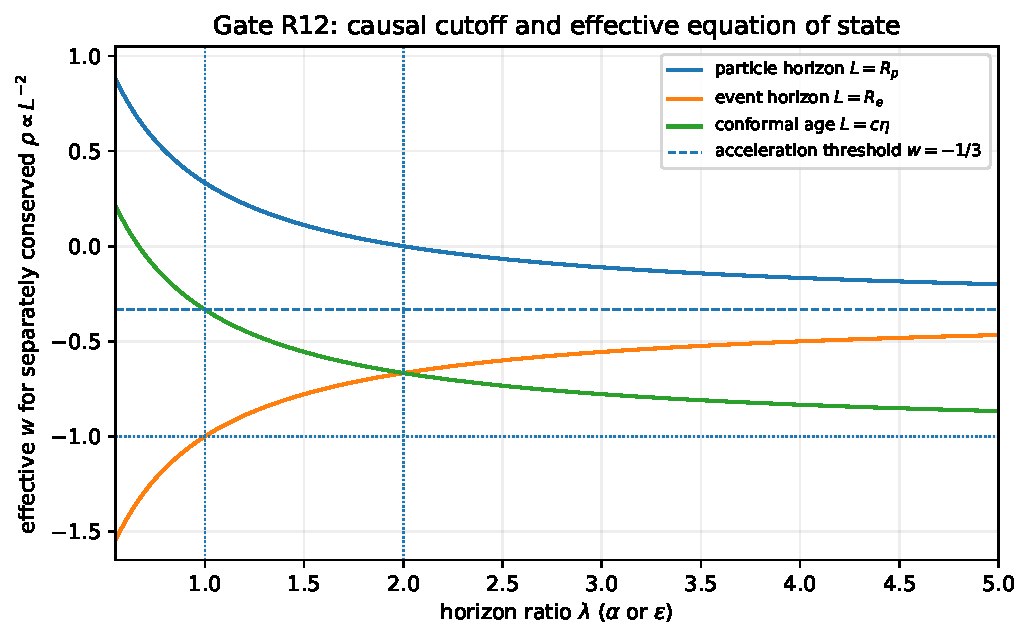
\includegraphics[width=0.84\textwidth]{causal_cutoff_eos.pdf}
\caption{Gate R12. Equazione di stato effettiva generata da tre cut-off $L^{-2}$. Il particle horizon resta sopra $w=-1/3$; l'event horizon e accelerante; il conformal-age cutoff puo diventare sufficientemente negativo pur usando solo il passato, ma appartiene a una classe con ipotesi microfisica aggiuntiva.}
\label{fig:r12_cutoff_eos}
\end{figure}

\subsection{Toy simmetrico passato--futuro}

Per verificare se la coppia $(\alpha,\varepsilon)$ possa chiudere da sola la dinamica, consideriamo deliberatamente un toy model minimale e non rivendicato come nuovo:
\begin{equation}
 \rho_\Sigma=\frac{3C^2c^2}{8\pi G}
 \left(\frac{1}{R_p^2}+\frac{1}{R_e^2}\right).
 \label{eq:r12_symmetric_density}
\end{equation}
La classe di generalized holographic dark energy consente cut-off dipendenti da particle horizon, future horizon e loro derivate \cite{NojiriOdintsov2017}; la Eq.~\eqref{eq:r12_symmetric_density} va quindi trattata come controllo interno, non come pretesa di novita.

Se $\rho_\Sigma$ costituisce l'intera densita di un universo piatto, Friedmann impone
\begin{equation}
 \boxed{C^2\left(\alpha^{-2}+\varepsilon^{-2}\right)=1}.
 \label{eq:r12_symmetric_constraint}
\end{equation}
Derivando e usando $\alpha'=1-q\alpha$, $\varepsilon'=-1-q\varepsilon$, si ottiene
\begin{equation}
 \boxed{
 q=\frac{\alpha^{-3}-\varepsilon^{-3}}
 {\alpha^{-2}+\varepsilon^{-2}}
 }.
 \label{eq:r12_symmetric_q}
\end{equation}
Per $C=1$ e utile parametrizzare
\begin{equation}
 \alpha^{-1}=\cos\theta,
 \qquad
 \varepsilon^{-1}=\sin\theta,
\end{equation}
cosi che
\begin{equation}
 q=\cos^3\theta-\sin^3\theta,
 \qquad
 \theta'=\sin\theta\cos\theta(\sin\theta+\cos\theta).
\end{equation}
Il sistema interpola automaticamente
\begin{equation}
 q:\quad +1\longrightarrow-1,
\end{equation}
cioe da un limite radiativo a un limite de Sitter. Tuttavia il passaggio per $q=1/2$ non e un'era materiale stabile: numericamente l'intervallo $0.4<q<0.6$ dura soltanto
\begin{equation}
 \Delta N\equiv\Delta\ln a\simeq0.186,
\end{equation}
pari a un aumento del fattore di scala di appena $e^{\Delta N}\simeq1.20$, e in $q=1/2$ si trova $dq/dN\simeq-1.09$. Il toy model salta quindi troppo rapidamente attraverso il comportamento materiale.

\begin{figure}[ht]
\centering
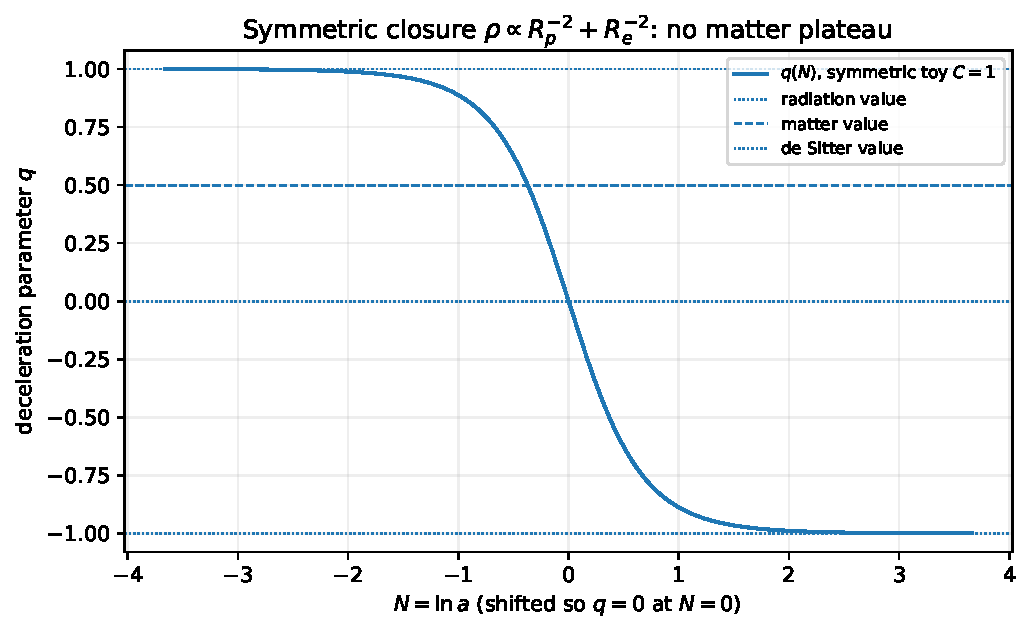
\includegraphics[width=0.84\textwidth]{symmetric_horizon_toy_q.pdf}
\caption{Toy simmetrico della Eq.~\eqref{eq:r12_symmetric_density} con $C=1$. L'interpolazione radiazione--de Sitter emerge, ma $q=1/2$ viene attraversato rapidamente e non forma una lunga era materiale.}
\label{fig:r12_symmetric_q}
\end{figure}

\subsection{Verdetto del Gate R12}

Il Gate R12 consente di classificare le chiusure minime in modo piu netto:
\begin{enumerate}
\item $R_p^{-2}$ e genuinamente legato al passato causale, ma traccia il background e non accelera;
\item $R_A^{-2}$ e locale ma, con coefficienti costanti, e una riscrittura della densita critica e non seleziona $q$;
\item $R_e^{-2}$ puo accelerare, ma usa una quantita globale definita dal futuro;
\item $\eta^{-2}$ puo essere piccolo nelle ere iniziali e dominante tardi, ma coincide con una classe agegrafica nota e richiede un principio aggiuntivo che giustifichi l'uso della scala conforme;
\item una combinazione simmetrica $R_p^{-2}+R_e^{-2}$ chiude un toy model elegante ma non riproduce una lunga era materiale e resta future-dependent.
\end{enumerate}

Il risultato piu utile e un no-go ristretto: una sorgente totale costruita con coefficienti costanti soltanto da $R_p^{-2}$ e $R_A^{-2}$ non puo generare la storia cosmologica completa. Per superarlo e necessario almeno uno fra: coefficienti dinamici, interazioni, derivate delle scale, una nuova scala temporale come $\eta$, un termine future-dependent, oppure una modifica della gravita. Ognuna di queste opzioni introduce nuova informazione fisica e deve essere motivata indipendentemente, non scelta per il fit.

\textbf{Gate R12:} \status{MINIMAL CAUSAL-ENERGY CLOSURE FAIL; CONFORMAL-AGE BENCHMARK SURVIVES WITH EXTRA PHYSICS}.



\section{Gate R12b: puo la prima luce selezionare la scala conforme?}

Il Gate R12 ha identificato $\eta^{-2}$ come primo benchmark basato esclusivamente sul passato capace di essere piccolo nelle ere iniziali e crescere tardivamente. La domanda successiva e piu severa: il tempo conforme puo essere selezionato dalla sola geometria causale dei raggi luminosi, oppure richiede una struttura di riferimento esterna?

\subsection{Liberta di normalizzazione FLRW}

Nel caso piatto,
\begin{equation}
 ds^2=-c^2dt^2+a^2(t)\left(d\chi^2+\chi^2d\Omega^2\right).
\end{equation}
La trasformazione costante
\begin{equation}
 \boxed{a(t)\longrightarrow\tilde a(t)=\lambda a(t),
 \qquad
 \chi\longrightarrow\tilde\chi=\frac{\chi}{\lambda}}
 \label{eq:r12b_scale_gauge}
\end{equation}
non modifica la metrica fisica: e soltanto una diversa normalizzazione della coordinata comovente. Anche $H=\dot a/a$ resta invariato.

Il tempo conforme soddisfa
\begin{equation}
 d\eta=\frac{dt}{a(t)}.
\end{equation}
Sotto la Eq.~\eqref{eq:r12b_scale_gauge},
\begin{equation}
 \boxed{\eta\longrightarrow\tilde\eta=\frac{\eta}{\lambda}}
 \label{eq:r12b_eta_scaling}
\end{equation}
a parita della scelta dell'origine temporale. Al contrario,
\begin{equation}
 R_p=ac\eta
 \quad\Longrightarrow\quad
 \tilde R_p=(\lambda a)c\frac{\eta}{\lambda}=R_p.
\end{equation}
Anche
\begin{equation}
 \alpha=\frac{HR_p}{c}=aH\eta
\end{equation}
e invariante.

Ne segue che una legge fondamentale
\begin{equation}
 \rho\propto\eta^{-2}
\end{equation}
non e, da sola, invariante rispetto alla normale liberta di riscalare $a$ e $\chi$:
\begin{equation}
 \eta^{-2}\longrightarrow\lambda^2\eta^{-2}.
\end{equation}
Per renderla fisica occorre fissare una normalizzazione, introdurre una quantita che trasformi compensando $\lambda$, oppure specificare una boundary condition fisicamente distinta. La convenzione cosmologica $a_0=1$ e perfettamente lecita per calcolare osservabili, ma non costituisce di per se una derivazione microfisica di una densita fondamentale.

Questo non invalida i modelli agegrafici come modelli fenomenologici. Stabilisce soltanto che la loro scala conforme non segue dalla sola struttura causale che aveva motivato il presente progetto.

\subsection{Perche una scala affine nulla non risolve il problema}

Si potrebbe tentare di sostituire $\eta$ con un parametro affine $\lambda_{\rm aff}$ lungo la geodetica nulla. Tuttavia un parametro affine possiede la liberta
\begin{equation}
 \lambda_{\rm aff}\longrightarrow A\lambda_{\rm aff}+B.
\end{equation}
Senza una normalizzazione fisica di $A$, una quantita come $\lambda_{\rm aff}^{-2}$ non definisce un'energia assoluta. Analogamente, l'espansione di una congruenza nulla dipende dalla normalizzazione del vettore tangente $k^\mu$; l'area fisica della sezione trasversa, invece, e invariante e riporta a scale proprie come $R_p$, gia sottoposte al no-go del Gate R12.

Il punto concettuale e che la struttura dei coni di luce determina il \emph{causal order} e le traiettorie nulle, ma non fissa da sola la scala conforme metrica necessaria per produrre una densita con dimensioni fisiche.

\subsection{No-go ristretto per una densita passata senza nuova scala}

Nel caso piatto, se non si introducono nuove scale dimensionali, la densita critica
\begin{equation}
 \rho_c=\frac{3H^2}{8\pi G}
\end{equation}
fornisce la scala naturale di densita. Una vasta classe di proposte costruite soltanto con il passato causale puo allora essere scritta come
\begin{equation}
 \boxed{\rho_X=\rho_c\,F(\alpha,\alpha',q,\ldots)},
 \label{eq:r12b_general_past_density}
\end{equation}
dove gli argomenti sono invarianti e adimensionali e il primo indica derivata rispetto a $\ln a$.

Durante una esatta era di potenza con equazione di stato costante,
\begin{equation}
 q=\mathrm{costante},
 \qquad
 \alpha=\frac1q=\mathrm{costante},
 \qquad
 \alpha'=0,
\end{equation}
e analogamente tutte le derivate finite di questi rapporti sono costanti o nulle. Di conseguenza
\begin{equation}
 \boxed{\Omega_X\equiv\frac{\rho_X}{\rho_c}=F(\mathrm{costanti})=\mathrm{costante}}.
 \label{eq:r12b_tracking_theorem}
\end{equation}
Il componente non puo quindi crescere da una frazione trascurabile a una frazione dominante durante una lunga era materiale esatta: traccia necessariamente il background.

Il risultato comprende come caso particolare $F=C^2/\alpha^2$, cioe il particle-horizon holographic cutoff. Per ottenere una crescita secolare della frazione energetica occorre almeno uno dei seguenti ingredienti:
\begin{enumerate}
\item una nuova scala dimensionale fissa, per esempio un rapporto $\mu/H$;
\item una variabile dinamica indipendente (campo, condensato, nuovo grado di liberta);
\item uno scambio energetico con altri settori;
\item una memoria non locale con una boundary condition fisica;
\item un input future-dependent come $R_e$;
\item una modifica delle equazioni gravitazionali.
\end{enumerate}
La causalita nulla e $c$ da sole non selezionano quale di questi ingredienti debba esistere.

\subsection{Una forma invariante del problema della scala conforme}

Si puo rendere esplicito il problema introducendo una epoca di riferimento $t_*$ e la quantita
\begin{equation}
 \eta_*(t)=\int_0^t\frac{a(t_*)}{a(t')}dt'.
\end{equation}
Il rapporto $a(t_*)/a(t')$ e invariante sotto la Eq.~\eqref{eq:r12b_scale_gauge}; $\eta_*$ e quindi fisicamente definibile una volta scelta $t_*$. Ma proprio questa scelta contiene la nuova informazione. Se $t_*=t$, allora
\begin{equation}
 c\eta_*(t)=R_p(t)
\end{equation}
e si ritorna al particle horizon. Se $t_*$ e ``oggi'', la legge fondamentale dipende dall'epoca dell'osservatore; se $t_*$ e una transizione microfisica, quella transizione diventa il nuovo input fisico. Non emerge una scelta privilegiata dalla sola geodetica della prima luce.

\subsection{Verdetto del Gate R12b}

Il ramo agegrafico resta utile come benchmark perche dimostra che una variabile integrata sul passato puo produrre accelerazione senza un future event horizon. Tuttavia il fattore che lo rende diverso da $R_p^{-2}$ non e selezionato dalla struttura causale FLRW: richiede una normalizzazione o una fisica aggiuntiva.

Il Gate produce quindi due conclusioni:
\begin{enumerate}
\item \textbf{ostacolo di scala conforme:} $\eta^{-2}$ non puo essere derivata come densita scalare dalla sola normalizzazione-libera geometria dei raggi nulli;
\item \textbf{tracking theorem ristretto:} ogni componente della forma Eq.~\eqref{eq:r12b_general_past_density}, senza nuova scala o grado di liberta, mantiene frazione costante in una esatta era di potenza e non puo generare da solo un takeover tardivo.
\end{enumerate}

\textbf{Gate R12b:} \status{CONFORMAL-SCALE ORIGIN NOT DERIVED; PAST-ONLY SCALE-FREE TRACKING NO-GO}.



\section{Gate R12c: una sola nuova scala fisica}

Il Gate R12b ha mostrato che una costruzione passata, scale-free e basata soltanto su $H$, $R_p$ e rapporti adimensionali non puo produrre un takeover tardivo durante una lunga era di potenza. Il primo ingrediente aggiuntivo da testare e quindi il piu parsimonioso possibile: \emph{una sola lunghezza fisica costante} $L_*$, nessun nuovo campo dinamico, nessuna interazione tra settori e nessun fit osservativo in questa fase.

\subsection{Famiglia monomiale minima}

Una densita con dimensione corretta costruita soltanto da $R_p$ e $L_*$ puo essere parametrizzata come
\begin{equation}
 \rho_X^{(n)}=
 \frac{3c^2}{8\pi G}\,
 L_*^{\,n-2}R_p^{-n},
 \label{eq:r12c_family}
\end{equation}
con $n$ costante. Il coefficiente unitario e scelto qui solo per eliminare un parametro ridondante: un coefficiente moltiplicativo potrebbe essere riassorbito in $L_*$ per $n\neq2$.

Durante una esatta era decelerante di potenza $a\propto t^p$ con $0<p<1$, l'orizzonte delle particelle e proporzionale a $t$ e la densita critica scala come $t^{-2}$. Pertanto
\begin{equation}
 \Omega_X\equiv\frac{\rho_X}{\rho_c}\propto t^{2-n}.
 \label{eq:r12c_tracking_break}
\end{equation}
Ne segue una classificazione immediata:
\begin{align}
 n<2 &: \quad \Omega_X\ \text{cresce},\\
 n=2 &: \quad \Omega_X\ \text{traccia il background},\\
 n>2 &: \quad \Omega_X\ \text{decresce}.
\end{align}
Quindi una singola scala dimensionale e sufficiente, matematicamente, a rompere il tracking theorem del Gate R12b.

Se la componente e conservata separatamente,
\begin{equation}
 \dot\rho_X+3H(1+w_X)\rho_X=0,
\end{equation}
la relazione $\dot R_p=HR_p+c$ fornisce
\begin{equation}
 \boxed{\quad
 w_X=-1+\frac{n}{3}\left(1+\frac1\alpha\right),
 \qquad \alpha=\frac{HR_p}{c}.
 \quad}
 \label{eq:r12c_w}
\end{equation}
Durante radiazione ($\alpha=1$) e materia ($\alpha=2$), rispettivamente,
\begin{equation}
 w_X^{(r)}=-1+\frac{2n}{3},
 \qquad
 w_X^{(m)}=-1+\frac n2.
\end{equation}
Le frazioni crescono come
\begin{equation}
 \Omega_X\propto a^{4-2n}
 \quad\text{(radiazione)},
 \qquad
 \Omega_X\propto a^{3-3n/2}
 \quad\text{(materia)}.
 \label{eq:r12c_growth_eras}
\end{equation}

\subsection{Tre casi strutturalmente distinti}

Il caso $n=2$ coincide con la densita $R_p^{-2}$ gia esclusa come tracker nel Gate R12. Il caso $n=0$ elimina invece ogni dipendenza da $R_p$:
\begin{equation}
 \rho_X^{(0)}=\frac{3c^2}{8\pi G L_*^2}=\mathrm{costante},
\end{equation}
cioe una costante cosmologica riscritta mediante la lunghezza $L_*$. Essa rompe il tracking, ma non conserva il contenuto causale dell'idea della prima luce.

Il primo monomio positivo che usa davvero entrambe le scale e $n=1$:
\begin{equation}
 \boxed{\quad
 \rho_X=\frac{3c^2}{8\pi G}\frac{1}{L_*R_p}.
 \quad}
 \label{eq:r12c_n1_density}
\end{equation}
In tal caso
\begin{equation}
 w_X=-\frac23+\frac{1}{3\alpha}.
 \label{eq:r12c_n1_w}
\end{equation}
Durante radiazione $w_X=-1/3$ e $\Omega_X\propto a^2$; durante materia $w_X=-1/2$ e $\Omega_X\propto a^{3/2}$. Una componente inizialmente trascurabile puo quindi diventare importante senza usare il future event horizon.

Se essa domina asintoticamente, l'accelerazione rende finita la parte futura dell'integrale conforme e $R_p\propto a$ a tempi tardi. Da $\rho_X\propto R_p^{-1}\propto a^{-1}$ segue $w_X\to-2/3$ e, nelle equazioni di Friedmann standard,
\begin{equation}
 \boxed{\quad a(t)\propto t^2,\qquad q\to-\frac12.\quad}
 \label{eq:r12c_n1_attractor}
\end{equation}
Piu in generale, per $0<n<2$ il ramo dominato da $X$ tende formalmente a
\begin{equation}
 a(t)\propto t^{2/n},
 \qquad
 q_\infty=\frac n2-1,
 \label{eq:r12c_general_attractor}
\end{equation}
mentre $n=0$ rappresenta separatamente il limite de Sitter.

\subsection{Controllo dinamico senza fit}

Per il caso $n=1$ il sistema di background piatto puo essere scritto, con $N=\ln a$, come
\begin{align}
 \alpha'&=1-q\alpha,\\
 \Omega_r'&=2\Omega_r(q-1),\\
 \Omega_X'&=\Omega_X\left[2(1+q)-\left(1+\frac1\alpha\right)\right],\\
 q&=\frac12\left[1+\Omega_r+3w_X\Omega_X\right],
 \qquad
 \Omega_m=1-\Omega_r-\Omega_X.
 \label{eq:r12c_autonomous}
\end{align}
La Fig.~\ref{fig:r12c_fractions} usa condizioni iniziali puramente illustrative, $\alpha_i=1$, $\Omega_{r,i}=0.999$, $\Omega_{X,i}=10^{-10}$, senza calibrare alcun osservabile attuale. Il sistema produce una lunga fase radiativa, una fase in cui la materia raggiunge $\Omega_m\simeq0.962$, e infine il takeover della componente $X$. Il parametro di decelerazione tende numericamente a $-1/2$, in accordo con Eq.~\eqref{eq:r12c_n1_attractor}. Lo spostamento orizzontale dell'epoca di takeover e controllato da $L_*$ e dalle condizioni iniziali, non e una predizione assoluta del modello.

\begin{figure}[htbp]
\centering
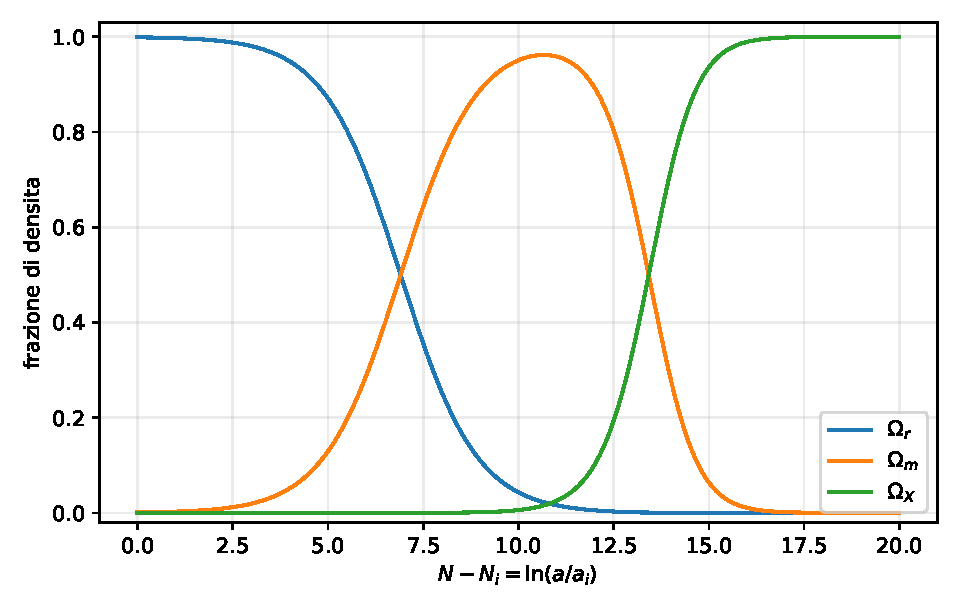
\includegraphics[width=0.79\textwidth]{r12c_n1_fractions.pdf}
\caption{Gate R12c, benchmark $n=1$. Evoluzione illustrativa delle frazioni di densita senza fit ai dati. Una sola scala permette a $\Omega_X$ di crescere dopo le ere standard; la posizione assoluta della transizione non e predetta finche $L_*$ non viene determinata indipendentemente.}
\label{fig:r12c_fractions}
\end{figure}

\begin{figure}[htbp]
\centering
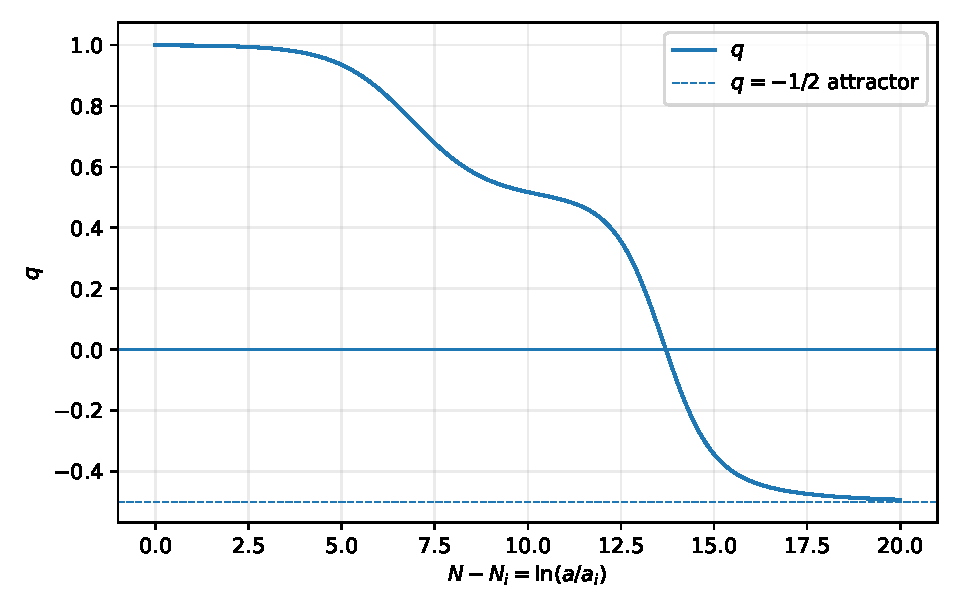
\includegraphics[width=0.79\textwidth]{r12c_n1_q.pdf}
\caption{Nello stesso controllo illustrativo, $q$ passa da circa $1$ a circa $1/2$ e infine tende all'attrattore $q=-1/2$. Il grafico dimostra la possibilita dinamica della sequenza, non la sua compatibilita quantitativa con le osservazioni.}
\label{fig:r12c_q}
\end{figure}

\subsection{Il prezzo della nuova scala}

Il risultato positivo e limitato. In era radiativa, per $n=1$ e $\alpha\simeq1$,
\begin{equation}
 \Omega_X\simeq\frac{R_p}{L_*},
\end{equation}
mentre durante materia, con $\alpha\simeq2$,
\begin{equation}
 \Omega_X\simeq\frac{R_p}{4L_*}.
\end{equation}
Il takeover avviene quindi quando una scala causale cosmologica diventa confrontabile con $L_*$. Se $L_*$ viene semplicemente scelta per far coincidere questo evento con l'epoca osservata di accelerazione, il problema della coincidenza non e spiegato: viene trasferito nella scelta di $L_*$. Inoltre la sola introduzione della scala non seleziona l'esponente $n$; scegliere $n$ costituisce ulteriore informazione fisica adimensionale.

\subsection{Controllo di novita: equivalenza con Tsallis HDE}

La famiglia della Eq.~\eqref{eq:r12c_family} non e nuova in senso fenomenologico. Nella Tsallis holographic dark energy con particle horizon la densita assume la forma
\begin{equation}
 \rho_D=B R_p^{2\delta-4}
\end{equation}
\cite{Zadeh2018}. Identificando gli esponenti,
\begin{equation}
 -n=2\delta-4
 \quad\Longrightarrow\quad
 \delta=2-\frac n2.
\end{equation}
Il nostro benchmark $n=1$ corrisponde quindi esattamente a
\begin{equation}
 \boxed{\delta=\frac32.}
\end{equation}
La letteratura ha gia mostrato che la modifica Tsallis puo consentire accelerazione anche usando il particle horizon, a differenza dell'HDE standard \cite{Zadeh2018}. Questo elimina qualunque rivendicazione di novita per la sola Eq.~\eqref{eq:r12c_n1_density}. Inoltre un'analisi del 2026 sulla crescita delle strutture trova che i modelli Tsallis con particle horizon sono in generale molto piu problematici di quelli con future event horizon \cite{Das2026}; il test perturbativo specifico del benchmark $n=1$ resta comunque da eseguire nel nostro workflow prima di un verdetto definitivo.

\subsection{Verdetto del Gate R12c}

Una sola scala dimensionale supera il no-go scale-free in senso matematico: esistono chiusure passate per cui la nuova componente e trascurabile nelle ere iniziali e cresce successivamente. Tuttavia il gate non fornisce una derivazione unica:
\begin{enumerate}
\item $n=0$ e semplicemente una costante cosmologica;
\item $n=1$ e il piu semplice monomio genuinamente causale ma appartiene a una classe Tsallis HDE gia nota;
\item il valore di $L_*$ non e determinato da causalita, $c+c$, termodinamica standard o geometria FLRW;
\item il valore di $n$ non e selezionato dalla sola introduzione della scala;
\item la classe particle-horizon generalizzata possiede gia vincoli di stabilita e crescita della struttura che impediscono di considerare il successo di background come sufficiente.
\end{enumerate}

\textbf{Gate R12c:} \status{ONE SCALE BREAKS TRACKING; UNIQUE CLOSURE NOT DERIVED; MINIMAL CAUSAL MONOMIAL IS KNOWN THDE}.


\section{Gate R12d: interazione covariante o memoria causale}

Il Gate R12c ha mostrato che una nuova scala fisica puo rompere il tracking, ma non viene selezionata dalla sola causalita. Il passo successivo e verificare due alternative piu dinamiche: (i) una singola interazione tra materia e componente causale; (ii) una memoria covariante retarded che integri il passato senza usare il future event horizon. L'obiettivo resta fail-closed: nessuna funzione di interazione o kernel viene adattato ai dati in questo gate.

\subsection{Interazione generica con la componente $R_p^{-2}$}

Si torna anzitutto alla densita holografica standard costruita sul particle horizon,
\begin{equation}
 \rho_p=\frac{3C^2c^2}{8\pi G R_p^2},
 \qquad
 \Omega_p=\frac{C^2}{\alpha^2},
 \qquad
 \alpha=\frac{HR_p}{c}.
 \label{eq:r12d_rhop}
\end{equation}
Si permetta uno scambio locale di energia con materia non relativistica,
\begin{align}
 \dot\rho_m+3H\rho_m&=Q,\\
 \dot\rho_p+3H(1+w_p)\rho_p&=-Q.
 \label{eq:r12d_continuity}
\end{align}
La definizione geometrica di $\rho_p$ e l'identita $\dot R_p=HR_p+c$ fissano comunque
\begin{equation}
 \frac{\dot\rho_p}{\rho_p}=-2H\left(1+\frac1\alpha\right).
\end{equation}
Introducendo
\begin{equation}
 \mathcal I\equiv\frac{Q}{3H\rho_p},
\end{equation}
segue
\begin{equation}
 \boxed{\quad
 w_p=-\frac13+\frac{2}{3\alpha}-\mathcal I.
 \quad}
 \label{eq:r12d_wp_interacting}
\end{equation}
L'interazione puo dunque rendere la pressione efficace piu negativa. Tuttavia la relazione tra frazione energetica e geometria resta indipendente da $Q$:
\begin{equation}
 \boxed{\quad
 \frac{\Omega_p'}{\Omega_p}
 =-2\frac{\alpha'}{\alpha}
 =2\left(q-\frac1\alpha\right),
 \qquad ' \equiv \frac{d}{d\ln a}.
 \quad}
 \label{eq:r12d_omega_identity}
\end{equation}
Poiche $\alpha>0$, durante qualunque fase accelerata $q<0$ si ha necessariamente
\begin{equation}
 \boxed{\quad q<0\quad\Longrightarrow\quad \Omega_p'<0.\quad}
 \label{eq:r12d_accel_fraction_decreases}
\end{equation}
Questa e una restrizione forte: la componente standard $R_p^{-2}$ non puo essere contemporaneamente la frazione che cresce fino a dominare e la sorgente di una fase accelerata. Se un'interazione produce accelerazione, il motore e lo scambio energetico stesso o il settore con cui avviene lo scambio, non un takeover del particle horizon.

Nel caso piatto materia+$p$,
\begin{equation}
 q=\frac12\left[1+3\Omega_p w_p\right],
\end{equation}
e la condizione $q<0$ richiede
\begin{equation}
 \boxed{\quad
 \mathcal I>
 \frac{1-\Omega_p}{3\Omega_p}
 +\frac{2}{3\alpha}.
 \quad}
 \label{eq:r12d_interaction_threshold}
\end{equation}
Quindi l'accelerazione puo essere ottenuta scegliendo un'interazione sufficientemente forte, ma la soglia non determina la forma di $Q$. Le forme comunemente studiate, ad esempio $Q=3\beta H\rho_p$, $3\beta H\rho_m$ o combinazioni delle due densita, introducono una costante adimensionale $\beta$ o una funzione equivalente; questa liberta e ben nota nella letteratura sui modelli HDE interagenti \cite{FengZhang2016,WangWangLi2017}.

\subsection{Il flusso naturale del bordo non e una nuova interazione}

L'idea della ``prima luce'' suggerisce un candidato apparentemente privo di parametri. Il particle horizon si muove rispetto al fluido comovente con velocita propria
\begin{equation}
 \dot R_p-HR_p=c.
\end{equation}
Per una sfera di volume $V_p=4\pi R_p^3/3$, la quantita di energia di un fluido omogeneo contenuta nel volume e $E=\rho V_p$. Usando la conservazione locale $\dot\rho=-3H(\rho+p)$ si trova
\begin{align}
 \dot E
 &=V_p\dot\rho+\rho\dot V_p\\
 &=-3HpV_p+4\pi R_p^2 c\,\rho.
 \label{eq:r12d_reynolds}
\end{align}
Il termine
\begin{equation}
 \Phi_{\rm sweep}=4\pi R_p^2c\,\rho
\end{equation}
e precisamente l'energia della materia che il bordo causale, avanzando di $c$ rispetto al fluido, ingloba nel volume di controllo. Dividendo per $V_p$ si ottiene formalmente
\begin{equation}
 \frac{\Phi_{\rm sweep}}{V_p}=\frac{3c\rho}{R_p}=\frac{3H\rho}{\alpha}.
 \label{eq:r12d_sweep_rate}
\end{equation}
Questa espressione assomiglia a un termine di interazione $Q$, ma non lo e: deriva gia dalla combinazione tra continuita locale e moto del bordo. Inserirla nuovamente nella continuita come sorgente microscopica conterebbe due volte lo stesso trasporto attraverso un volume mobile. Il ``flusso della prima luce'' e quindi un'identita di bilancio del volume causale, non una legge di scambio indipendente tra settori.

\subsection{Memoria covariante dimensionale: nuovo kernel, stesso tracking}

Per evitare un ansatz locale per $Q$ si puo costruire una memoria retarded con l'operatore d'Alembertiano. Si consideri il piu semplice scalare causale
\begin{equation}
 -\Box U=1,
 \label{eq:r12d_boxU}
\end{equation}
con condizioni iniziali retarded $U=\dot U=0$ sulla superficie iniziale scelta. Per un campo omogeneo in FLRW piatto,
\begin{equation}
 \ddot U+3H\dot U=1.
\end{equation}
In una esatta era di potenza $a\propto t^p$ la soluzione particolare dominante e
\begin{equation}
 \boxed{\quad
 U(t)=\frac{t^2}{2(1+3p)}+\hbox{termini di bordo/decrescenti}.
 \quad}
 \label{eq:r12d_U_powerlaw}
\end{equation}
Una densita costruita senza una nuova scala come
\begin{equation}
 \rho_U=\kappa\frac{M_{\rm Pl}^2}{U}
\end{equation}
scala quindi come $t^{-2}$, esattamente come $H^2M_{\rm Pl}^2$. La sua frazione resta costante durante una era autosimile. Lo stesso risultato segue per la memoria data dal quattro-volume del passato causale: in un background di potenza il volume del cono passato scala dimensionalmente come $V_4\propto t^4$, e dunque $M_{\rm Pl}^2/\sqrt{V_4}\propto t^{-2}$. Il kernel retarded rende la costruzione causale, ma non rompe da solo l'autosimilarita responsabile del tracking.

\subsection{Memoria adimensionale secolare: rompe il tracking, non seleziona la dinamica}

Un comportamento diverso emerge con
\begin{equation}
 X=-\Box^{-1}R,
 \label{eq:r12d_X}
\end{equation}
anch'esso definito con Green retarded. Per $a\propto t^p$ e $k=0$,
\begin{equation}
 R=\frac{6p(2p-1)}{t^2}.
\end{equation}
Durante la radiazione ($p=1/2$), $R=0$ e la memoria resta quiescente se le condizioni iniziali sono nulle. Durante la materia ($p=2/3$), invece,
\begin{equation}
 X(t)=\frac43\ln t+\hbox{termini di bordo/decrescenti}
 \label{eq:r12d_X_matter_asymptotic}
\end{equation}
(a meno della scelta dell'origine del logaritmo). In un toy background con transizione istantanea a $t=t_{\rm eq}$ e $X=\dot X=0$ all'uguaglianza,
\begin{equation}
 X(t)=\frac43\left[\ln\frac{t}{t_{\rm eq}}+\frac{t_{\rm eq}}{t}-1\right],
 \qquad t\ge t_{\rm eq}.
 \label{eq:r12d_X_piecewise}
\end{equation}
La Fig.~\ref{fig:r12d_memory} mostra questa crescita secolare. Una memoria di questo tipo puo quindi introdurre un ``orologio'' adimensionale del passato e sfuggire al tracking theorem locale del Gate R12b.

\begin{figure}[htbp]
\centering
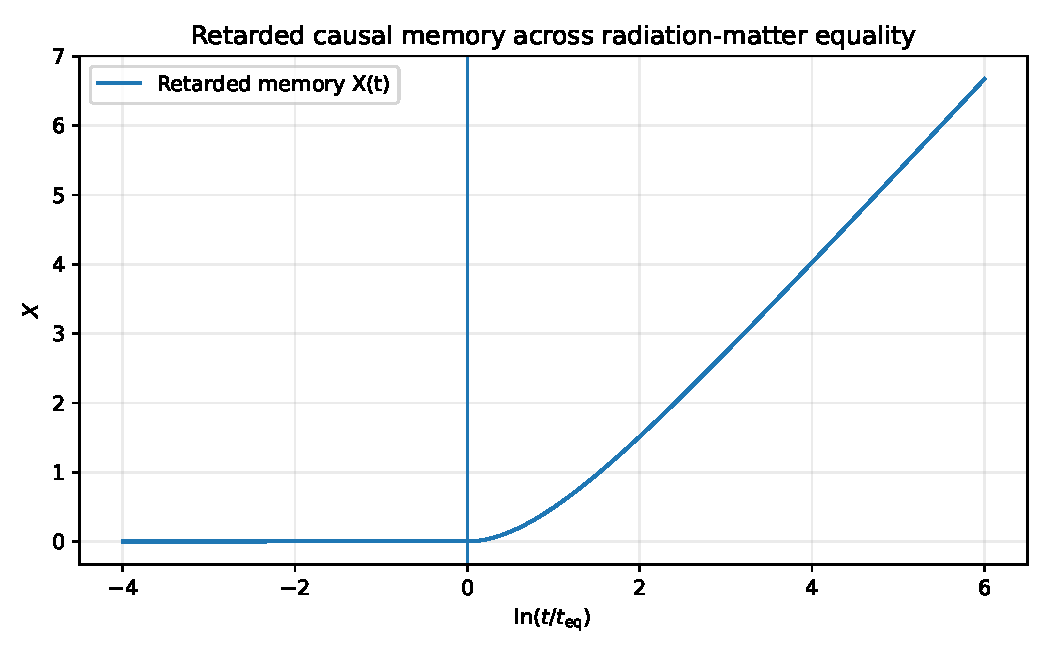
\includegraphics[width=0.76\textwidth]{r12d_retarded_memory.pdf}
\caption{Toy retarded memory $X=-\Box^{-1}R$ attraverso una transizione ideale radiazione--materia. Con condizioni iniziali nulle, $X$ resta fermo quando $R=0$ nell'era radiativa e cresce logaritmicamente in materia. Il grafico dimostra che una memoria causale adimensionale puo accumulare storia senza una nuova lunghezza; non specifica pero come $X$ debba entrare nelle equazioni gravitazionali.}
\label{fig:r12d_memory}
\end{figure}

Il problema di chiusura si sposta pero al passo successivo. Per trasformare $X$ in dinamica bisogna specificare una funzione o un accoppiamento, ad esempio un'azione del tipo $R f(X)$ oppure una densita efficace contenente una funzione $F(X)$. Questa funzione non e selezionata dal solo operatore retarded. Le costruzioni non locali di Deser e Woodard sfruttano precisamente memorie del tipo $\Box^{-1}R$ e varianti piu elaborate; nelle versioni fenomenologiche la funzione di distorsione viene scelta o ricostruita per ottenere la storia cosmologica desiderata \cite{DeserWoodard2007,DeserWoodard2019}. Una diversa classe, il modello ``RR'', introduce invece esplicitamente una nuova scala di massa in un termine $m^2R\Box^{-2}R$ \cite{MaggioreMancarella2014,MaggioreReview2016}. La memoria covariante e dunque fisicamente possibile e puo ritardare la risposta cosmologica, ma non elimina automaticamente il problema della selezione: o compare una funzione libera, o compare una nuova scala, o entrambe.

\subsection{Verdetto del Gate R12d}

I due rami portano allo stesso tipo di ostacolo da direzioni diverse:
\begin{enumerate}
\item una interazione $Q$ puo modificare la pressione efficace, ma la causalita del particle horizon non ne determina la forma o l'intensita;
\item per $\rho_p\propto R_p^{-2}$, ogni fase accelerata implica $\Omega_p'<0$, quindi l'accelerazione interagente non puo essere interpretata come takeover della componente causale standard;
\item il flusso dovuto al moto del bordo $R_p$ e un termine di trasporto di un volume mobile, non un nuovo scambio locale tra fluidi;
\item le memorie retarded dimensionali minime conservano il tracking nelle ere autosimili;
\item una memoria adimensionale come $-\Box^{-1}R$ puo crescere secolarmente e rompere il tracking, ma non determina da sola la funzione con cui modifica energia o gravita.
\end{enumerate}

\textbf{Gate R12d:} \status{COVARIANT INTERACTION/MEMORY CAN MODIFY TRACKING; CAUSALITY DOES NOT SELECT THE COUPLING; UNIQUE CLOSURE NOT DERIVED}.


\section{Gate R12e: congruenza nulla, Raychaudhuri e principio di selezione}

Il Gate R12d ha mostrato che interazioni e memorie retarded possono modificare la dinamica soltanto introducendo una coupling, una funzione o una scala addizionale. Il Gate R12e torna quindi al nucleo geometrico dell'idea iniziale: il fronte della ``prima luce'' come congruenza nulla. La domanda e se l'espansione ottica del fascio, la sua area e il focusing possano selezionare il contenuto energetico senza importare una legge ulteriore. In questa sezione si pongono temporaneamente $c=1$ e si ripristina $c$ nelle formule cinematiche finali.

\subsection{Raychaudhuri nulla e area del fascio}

Sia $k^\mu=dx^\mu/d\lambda$ il vettore tangente a una congruenza nulla parametrizzata affinalmente. Se $\mathcal A$ e l'area trasversa del fascio, la sua espansione ottica e
\begin{equation}
 \vartheta\equiv\frac{1}{\mathcal A}\frac{d\mathcal A}{d\lambda}.
 \label{eq:r12e_theta_def}
\end{equation}
L'equazione di Raychaudhuri nulla in quattro dimensioni e
\begin{equation}
 \frac{d\vartheta}{d\lambda}
 =-\frac12\vartheta^2-\sigma_{\mu\nu}\sigma^{\mu\nu}
 +\omega_{\mu\nu}\omega^{\mu\nu}
 -R_{\mu\nu}k^\mu k^\nu.
 \label{eq:r12e_null_raychaudhuri}
\end{equation}
Per un fascio radiale hypersurface-orthogonal in FLRW la vorticita e nulla; l'omogeneita, l'isotropia e la conformal flatness rendono nullo anche lo shear del fascio radiale ideale. Ponendo $\mathcal A=4\pi\mathcal R^2$, dove $\mathcal R$ e il raggio areale del fascio, si ha
\begin{equation}
 \vartheta=2\frac{\mathcal R'}{\mathcal R},
 \qquad{}'\equiv\frac{d}{d\lambda},
\end{equation}
e quindi
\begin{equation}
 \boxed{\quad
 \mathcal R''=-\frac12 R_{\mu\nu}k^\mu k^\nu\,\mathcal R.
 \quad}
 \label{eq:r12e_optical_radius}
\end{equation}
Questa e la forma di focusing che, in FLRW, coincide con la deviazione geodetica nulla standard \cite{EllisVanElst1997}.

\subsection{La congruenza nulla vede $\rho+p$, non $\rho+3p$}

Usando le equazioni di Einstein con un fluido perfetto,
\begin{equation}
 R_{\mu\nu}k^\mu k^\nu
 =8\pi G\,T_{\mu\nu}k^\mu k^\nu
 =8\pi G(\rho+p)(u\!\cdot\! k)^2,
 \label{eq:r12e_Rkk_fluid}
\end{equation}
perche sia il termine di traccia sia un termine $\Lambda g_{\mu\nu}$ si annullano quando vengono contratti con un vettore nullo. Ne segue
\begin{equation}
 \boxed{\quad
 \mathcal R''=-4\pi G(\rho+p)(u\!\cdot\! k)^2\,\mathcal R.
 \quad}
 \label{eq:r12e_focusing_rhop}
\end{equation}
Il focusing ottico e quindi controllato dalla combinazione $\rho+p$, cioe dalla null energy condition, e non dalla active gravitational mass $\rho+3p$ che compare nell'equazione di accelerazione cosmica.

Per FLRW con curvatura spaziale $k$, la stessa contrazione geometrica puo essere scritta come
\begin{equation}
 R_{\mu\nu}k^\mu k^\nu
 =2\left(\frac{k}{a^2}-\dot H\right)(k^t)^2.
 \label{eq:r12e_Rkk_Hdot}
\end{equation}
Confrontando le due forme si recupera
\begin{equation}
 \boxed{\quad
 \dot H-\frac{k}{a^2}=-4\pi G(\rho+p).
 \quad}
 \label{eq:r12e_derivative_friedmann}
\end{equation}
Quindi la Raychaudhuri nulla non produce una nuova equazione cosmologica: ricostruisce precisamente la combinazione derivativa di Friedmann gia contenuta nelle equazioni di Einstein.

\subsection{Il punto $c+c$ sull'orizzonte apparente}

La geometria ottica chiarisce tuttavia un punto direttamente connesso all'intuizione originaria. Nel caso piatto, per un raggio radiale
\begin{equation}
 \frac{dR_\pm}{dt}=HR_\pm\pm c.
\end{equation}
L'orizzonte apparente coincide con
\begin{equation}
 R_A=\frac{c}{H}.
\end{equation}
Valutando i due raggi sulla stessa sfera $R=R_A$ si ottiene esattamente
\begin{align}
 \left.\frac{dR_+}{dt}\right|_{R_A}&=c+c=\boxed{2c},\\
 \left.\frac{dR_-}{dt}\right|_{R_A}&=c-c=\boxed{0}.
 \label{eq:r12e_horizon_null_rates}
\end{align}
Il primo risultato non e una somma relativistica di velocita locali: e la variazione del raggio areale rispetto al tempo cosmico, con un contributo locale $c$ e uno geometrico $HR_A=c$. Il secondo e la consueta caratterizzazione dell'orizzonte apparente attraverso l'annullamento dell'espansione del ramo entrante.

L'orizzonte stesso, invece, evolve secondo
\begin{equation}
 \dot R_A=c(1+q)
 \label{eq:r12e_RA_rate}
\end{equation}
nel caso piatto. Pertanto il raggio uscente sull'orizzonte ha sempre tasso areale $2c$, mentre l'orizzonte si muove allo stesso tasso soltanto quando
\begin{equation}
 q=1,
\end{equation}
cioe nell'era radiativa ideale. In quella fase coincidono anche $R_p=R_A=2ct$: questa e la ragione geometrica precisa per cui il ``primo fronte'' radiativo realizza il caso $c+c$ gia emerso nei Gate precedenti.

\subsection{Vacuum blindness: de Sitter non focalizza il fascio nullo}

Per una componente di vuoto
\begin{equation}
 p=-\rho,
\end{equation}
si ha
\begin{equation}
 \rho+p=0
 \qquad\Longrightarrow\qquad
 R_{\mu\nu}k^\mu k^\nu=0.
\end{equation}
Lo stesso vale direttamente per una costante cosmologica, poiche $g_{\mu\nu}k^\mu k^\nu=0$. In de Sitter FLRW, inoltre, il tensore di Weyl e nullo; la Eq.~\eqref{eq:r12e_optical_radius} diventa quindi
\begin{equation}
 \boxed{\mathcal R''=0}
 \label{eq:r12e_desitter_affine}
\end{equation}
rispetto al parametro affine, pur avendo
\begin{equation}
 a(t)\propto e^{Ht},\qquad q=-1.
\end{equation}
La stessa equazione di focusing affine vale per un fascio radiale in Minkowski. L'espansione accelerata de Sitter e quindi invisibile al termine locale di Ricci focusing della congruenza nulla. Questo e un no-go diretto per qualunque tentativo di determinare l'accelerazione tipo dark energy usando soltanto $R_{\mu\nu}k^\mu k^\nu$ della prima luce.

\subsection{L'integrazione lascia libera una costante cosmologica}

Aggiungendo la conservazione locale
\begin{equation}
 \dot\rho+3H(\rho+p)=0
 \label{eq:r12e_conservation}
\end{equation}
alla Eq.~\eqref{eq:r12e_derivative_friedmann}, si trova
\begin{equation}
 \frac{d}{dt}\left[
 H^2+\frac{k}{a^2}-\frac{8\pi G}{3}\rho
 \right]=0.
\end{equation}
Pertanto
\begin{equation}
 \boxed{\quad
 H^2+\frac{k}{a^2}=\frac{8\pi G}{3}\rho+C,
 \quad}
 \label{eq:r12e_friedmann_constant}
\end{equation}
dove $C$ e una costante di integrazione; nella notazione di Einstein puo essere identificata con $\Lambda/3$. La congruenza nulla determina quindi la parte differenziale della dinamica, ma non il settore proporzionale alla metrica.

Questo e esattamente il tipo di liberta che compare nella derivazione termodinamica di Jacobson: imponendo Clausius su tutti gli orizzonti causali locali si ottengono le equazioni di Einstein con una costante cosmologica non determinata \cite{Jacobson1995}. Analogamente, formulazioni entropiche direttamente su superfici nulle recuperano Einstein/Lovelock con $\Lambda$ come costante di integrazione \cite{PadmanabhanParanjape2007}. R12e non scopre quindi una nuova chiusura; identifica con precisione quale informazione la geometria nulla non puo selezionare.

\subsection{La boundary condition della ``prima luce'' puo fissare $C$?}

Il particle horizon parte da area nulla nel limite iniziale standard,
\begin{equation}
 R_p\to0,\qquad \mathcal A_p\to0,
\end{equation}
ma questa condizione e condivisa da un'intera famiglia di cosmologie e non fissa $C$. Inoltre la normalizzazione affine possiede la liberta $\lambda\to A\lambda+B$, per cui il valore iniziale di $d\mathcal R/d\lambda$ non costituisce da solo una scala fisica assoluta.

Nel regime radiativo standard,
\begin{equation}
 \rho_r\propto a^{-4},
\end{equation}
mentre qualunque $C$ finito rimane costante. Quindi
\begin{equation}
 \frac{C}{(8\pi G/3)\rho_r}\longrightarrow0
 \qquad (a\to0).
 \label{eq:r12e_early_constant_hidden}
\end{equation}
Le condizioni asintotiche locali vicino al Big Bang non distinguono pertanto valori finiti differenti della costante di integrazione. Piu fortemente, il contributo di vuoto resta assente da $\rho+p$ a ogni epoca. Ne segue un no-go ristretto:
\begin{quote}
la Raychaudhuri nulla, la conservazione locale e la sola boundary condition locale del fronte causale primordiale non selezionano il valore della costante cosmologica.
\end{quote}
Una selezione richiederebbe un principio globale, una boundary condition addizionale, una nuova dinamica del vuoto oppure un input osservativo a tempo finito.

\subsection{Verdetto del Gate R12e}

Il gate produce due risultati distinti. Il primo e positivo sul piano interpretativo: il $c+c$ compare in modo esatto per un raggio uscente istantaneamente posto sull'orizzonte apparente piatto, e nell'era radiativa il particle horizon stesso coincide con quella scala e si muove anch'esso a $2c$. Il secondo e negativo sul piano dinamico: la Raychaudhuri nulla ricostruisce la combinazione $\dot H-k/a^2$, e quindi Friedmann solo fino a una costante, ma non vede il settore di vuoto che potrebbe determinare l'accelerazione tardiva.

\textbf{Gate R12e:} \status{NULL RAYCHAUDHURI RECOVERS DERIVATIVE FRIEDMANN; VACUUM/LAMBDA BLIND; FIRST-LIGHT BOUNDARY DOES NOT SELECT THE INTEGRATION CONSTANT; UNIQUE CLOSURE NOT DERIVED}.

\section{Gate R12f: origine della costante di integrazione}

Il Gate R12e ha isolato il problema in forma molto precisa: la dinamica nulla determina la combinazione derivativa di Friedmann, ma lascia libera una costante $C=\Lambda c^2/3$. R12f testa quindi se un principio globale, ma non costruito a posteriori sui dati cosmologici, possa selezionare quel settore proporzionale alla metrica. I rami vengono classificati secondo tre domande: (i) il valore di $\Lambda$ e realmente determinato oppure soltanto ricodificato come dato di stato? (ii) serve informazione sull'intero futuro cosmico? (iii) compare una nuova scala, una misura esterna o una microstruttura addizionale?

\subsection{Causal diamond ed entanglement equilibrium}

L'ipotesi di entanglement equilibrium di Jacobson considera piccoli causal diamond/geodesic ball e postula la stazionarieta dell'entropia generalizzata del vuoto a volume fissato. Per variazioni di primo ordine il principio e equivalente alla equazione semiclassica di Einstein \cite{Jacobson2015}. La formulazione termodinamica dei causal diamond in spazi massimamente simmetrici rende pero esplicito il ruolo di $\Lambda$: la first law contiene un termine
\begin{equation}
 \delta H_\zeta^{\Lambda}=\frac{V_\zeta}{8\pi G}\,\delta\Lambda,
 \label{eq:r12f_diamond_lambda_work}
\end{equation}
e l'equilibrio entanglement standard e formulato a volume e cosmological constant fissati \cite{JacobsonVisser2019}. Il principio ricostruisce quindi la struttura delle equazioni gravitazionali attorno a un vuoto massimamente simmetrico, ma non seleziona il valore assoluto della curvatura di quel vuoto. Permettere $\delta\Lambda$ introduce una coppia termodinamica addizionale, non una equazione che ne determini il valore.

\textbf{Esito:} causal-diamond thermodynamics e entanglement equilibrium sono un controllo positivo della connessione causalita--gravita, ma non chiudono la costante lasciata libera da R12e.

\subsection{Unimodularita: la costante diventa un dato globale}

Nella forma classica della gravita unimodulare le equazioni possono essere scritte in forma traceless,
\begin{equation}
 R_{\mu\nu}-\frac14Rg_{\mu\nu}
 =8\pi G\left(T_{\mu\nu}-\frac14Tg_{\mu\nu}\right).
 \label{eq:r12f_unimodular_traceless}
\end{equation}
Usando la conservazione $\nabla^\mu T_{\mu\nu}=0$ e l'identita di Bianchi segue
\begin{equation}
 \nabla_\nu\left(R+8\pi G T\right)=0,
\end{equation}
quindi
\begin{equation}
 \boxed{R+8\pi G T=4\Lambda.}
 \label{eq:r12f_unimodular_constant}
\end{equation}
La costante cosmologica riappare pertanto come costante di integrazione. Nelle formulazioni covarianti tipo Henneaux--Teitelboim essa puo essere promossa a grado di liberta globale legato al volume spazio-temporale; questo modifica il suo status concettuale e puo rendere radiativamente naturale il settore di vuoto, ma non determina automaticamente il valore osservato. Revisioni moderne sottolineano che una soluzione del problema richiede una specifica scelta dei dati globali/iniziali e un vincolo sul quattro-volume \cite{Jirousek2023}; nella formulazione di boundary-state la piccolezza di $\Lambda$ resta una proprieta dello stato iniziale \cite{BuchmullerDragon2022}.

\textbf{Esito:} la unimodularita spiega perche $\Lambda$ possa essere una costante globale invece di un parametro locale dell'azione, ma R12f non trova un principio interno che ne scelga il valore.

\subsection{Vincoli sul quattro-volume e vacuum-energy sequestering}

Il vacuum-energy sequestering mostra che un vincolo globale sul quattro-volume puo cancellare la sensibilita della curvatura alle grandi correzioni di energia del vuoto. Nella proposta originale i parametri dimensionali del settore di materia dipendono funzionalmente dal volume quadridimensionale totale; per avere una soluzione non banale lo spazio-tempo deve essere finito e il modello originale prevede una futura ricollassazione \cite{KaloperPadilla2014}. Il meccanismo e quindi importante come prova di principio che un dato globale possa controllare il settore di vuoto, ma per il programma presente presenta due costi espliciti:
\begin{enumerate}
\item usa informazione globale sull'intera storia spazio-temporale, incluso il futuro nella formulazione originale;
\item introduce variabili/vincoli globali addizionali che non emergono dalla sola congruenza della prima luce.
\end{enumerate}
Le formulazioni locali con forme differenziali spostano la non-localita nelle condizioni globali e nei flux, ma non trasformano il valore residuo in una predizione della cinematica $HD\pm c$.

\textbf{Esito:} il sequestering puo affrontare la radiative stability del vuoto, ma non soddisfa il criterio ``solo passato causale, nessun nuovo dato globale'' adottato in questa esplorazione.

\subsection{Il ramo piu vicino alla ``prima luce'': quattro-volume del passato causale}

Esiste tuttavia una idea che combina direttamente unimodularita e struttura causale del passato: la proposta ``Everpresent $\Lambda$'' motivata dalla causal set theory. In un causal set il numero $N$ di elementi in una regione quattro-dimensionale fluttua come un processo di Poisson, $\Delta N\sim\sqrt N$; combinando questa discrezione con la coniugazione quantistica euristica tra $\Lambda$ e quattro-volume si ottiene, in un modello fenomenologico,
\begin{equation}
 \boxed{\Lambda_{\rm rms}\sim\frac{\xi}{\sqrt{V_4[J^-(x)]}}},
 \label{eq:r12f_everpresent_scaling}
\end{equation}
dove $V_4[J^-(x)]$ e il volume del passato causale dell'evento $x$ e $\xi$ e una ampiezza adimensionale che codifica la microfisica discreta \cite{AhmedEtAl2004,AhmedSorkin2012}. Questa costruzione e concettualmente piu vicina al progetto: non usa l'event horizon futuro e il volume cresce con la storia causale gia trascorsa.

La scala temporale puo essere analizzata esattamente nelle ere FLRW di potenza. Per un universo piatto
\begin{equation}
 a(t)=A t^p,\qquad 0<p<1,
\end{equation}
il quattro-volume del cono di luce passato, dal Big Bang all'evento $(t,\mathbf 0)$, e
\begin{equation}
 V_4(t)=\frac{4\pi c}{3}\int_0^t dt'\,a^3(t')
 \left[\int_{t'}^t\frac{c\,dt''}{a(t'')}\right]^3.
 \label{eq:r12f_v4_integral}
\end{equation}
L'integrale e elementare e fornisce
\begin{equation}
 \boxed{
 V_4(t)=\frac{\pi c^4t^4}{(1+p)(3+p)(1+3p)}.
 }
 \label{eq:r12f_v4_powerlaw}
\end{equation}
La normalizzazione $A$ scompare, come deve per una quantita geometrica fisica. Da Eq.~\eqref{eq:r12f_everpresent_scaling}, con $H=p/t$, segue
\begin{equation}
 \frac{\Lambda_{\rm rms}c^2}{H^2}
 =\frac{\xi}{p^2}
 \sqrt{\frac{(1+p)(3+p)(1+3p)}{\pi}},
 \label{eq:r12f_lambda_over_h2}
\end{equation}
e pertanto
\begin{equation}
 \boxed{
 \Omega_{\Lambda,{\rm rms}}
 =\frac{\Lambda_{\rm rms}c^2}{3H^2}
 =\frac{\xi}{3p^2}
 \sqrt{\frac{(1+p)(3+p)(1+3p)}{\pi}}.
 }
 \label{eq:r12f_omega_tracker}
\end{equation}
La frazione tipica e quindi \emph{costante} in ogni esatta era di potenza. In particolare,
\begin{align}
 p=\frac12 &: \quad \Omega_{\Lambda,{\rm rms}}\simeq2.725\,\xi,\\
 p=\frac23 &: \quad \Omega_{\Lambda,{\rm rms}}\simeq1.812\,\xi.
 \label{eq:r12f_radmatter_numbers}
\end{align}
La figura~\ref{fig:r12f_past_volume_tracker} mostra il coefficiente generale. Questa derivazione chiarisce perche la proposta viene chiamata ``ever-present'': il quattro-volume passato produce naturalmente una componente dell'ordine di $H^2$, cioe un tracker stocastico, non una costante piccola per quasi tutta la storia che diventa importante soltanto tardi.

\begin{figure}[htbp]
 \centering
 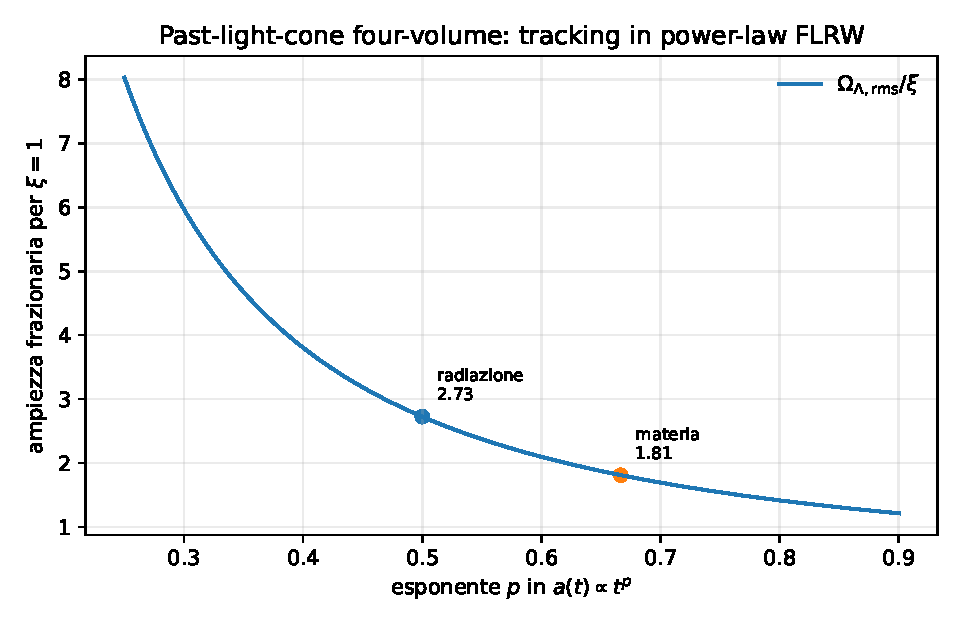
\includegraphics[width=0.72\textwidth]{r12f_past_volume_tracker.pdf}
 \caption{Per $a\propto t^p$, una legge stocastica $\Lambda_{\rm rms}=\xi/\sqrt{V_4}$ produce una frazione $\Omega_{\Lambda,{\rm rms}}$ indipendente dal tempo durante l'era di potenza. La microfisica entra nell'ampiezza $\xi$.}
 \label{fig:r12f_past_volume_tracker}
\end{figure}

Questo ramo non e pero una chiusura parameter-free. Le implementazioni note richiedono almeno una ampiezza fenomenologica e ipotesi supplementari; una analisi strutturale sottolinea esplicitamente che l'ampiezza non e ancora derivata da primi principi e che l'omogeneita spaziale delle fluttuazioni viene imposta nel modello fenomenologico \cite{AhmedSorkin2012}. Inoltre test piu recenti con supernovae e CMB trovano che le realizzazioni standard di Everpresent $\Lambda$ hanno difficolta con la CMB e che le fluttuazioni preferite dai dati sono piu piccole di quelle tipiche dei modelli correnti \cite{DasNasiriYazdi2023}.

\subsection{Cosa ha effettivamente selezionato R12f?}

I quattro rami producono una gerarchia chiara:
\begin{enumerate}
\item entanglement equilibrium seleziona la forma locale della dinamica, non il valore assoluto di $\Lambda$;
\item unimodularita ricodifica $\Lambda$ come costante/grado globale e sposta la selezione ai dati di stato o al quattro-volume;
\item sequestering usa con successo vincoli globali per neutralizzare l'energia del vuoto, ma richiede nuova struttura globale e, nella forma originale, l'intera storia futura;
\item causal-set discreteness e il solo ramo testato che usa direttamente il passato causale per produrre una \emph{scala} di $\Lambda$ senza event horizon, ma la scala e stocastica, traccia $H^2$ nelle ere di potenza e contiene ancora una ampiezza/microfisica non derivata.
\end{enumerate}

Quindi R12f non trova una selezione unica della costante $C$ di Eq.~\eqref{eq:r12e_friedmann_constant}. Trova pero un bivio piu preciso: una teoria puramente continua e locale lascia $C$ libero; per determinare o sostituire quel settore bisogna aggiungere almeno dati globali oppure microstruttura quantistica/discreta. Il candidato piu compatibile con il vincolo ``solo passato causale'' non genera una costante deterministica: genera fluttuazioni ever-present.

\subsection{Verdetto del Gate R12f}

\textbf{Gate R12f:} \status{GLOBAL/ENTANGLEMENT/UNIMODULAR CONDITIONS DO NOT UNIQUELY SELECT LAMBDA; PAST-FOUR-VOLUME CAUSAL-SET FLUCTUATIONS SET A STOCHASTIC SCALE BUT REQUIRE DISCRETE MICROPHYSICS AND PHENOMENOLOGICAL INPUT; UNIQUE CLOSURE NOT DERIVED}.


\section{Gate R12g: microstruttura causale, correlazioni e conservazione}

Il Gate R12f ha lasciato aperta una possibilita precisa: una microstruttura discreta del passato causale puo generare una scala stocastica $\Lambda_{\rm rms}\sim V_4^{-1/2}$ senza ricorrere all'event horizon. R12g chiede se, prendendo sul serio il contenuto discreto dei coni causali locali, si possano derivare (i) l'ampiezza, (ii) le correlazioni spazio-temporali e (iii) una legge covariante conservata, senza imporre omogeneita o kernel fenomenologici a mano.

\subsection{Ampiezza: il parametro puo essere reinterpretato, non eliminato}

Per uno sprinkling di densita causale $\rho_{\rm cs}=\ell_{\rm cs}^{-4}$, il numero di elementi in un volume $V$ soddisfa
\begin{equation}
 N\simeq \frac{V}{\ell_{\rm cs}^4},\qquad \delta N\simeq\sqrt N,
\end{equation}
e quindi
\begin{equation}
 \delta V\simeq \ell_{\rm cs}^2\sqrt V.
\end{equation}
Combinando questa relazione con la coniugazione euristica unimodulare tra $\Lambda$ e quattro-volume, le analisi moderne di Everpresent $\Lambda$ parametrizzano l'ampiezza tramite
\begin{equation}
 \boxed{\alpha_E\equiv\frac12\left(\frac{\ell_p}{\ell_{\rm cs}}\right)^2,}
 \label{eq:r12g_alphaE}
\end{equation}
con fluttuazioni del tipo
\begin{equation}
 \delta\Lambda\simeq \frac{8\pi\alpha_E}{\sqrt V}
 \label{eq:r12g_deltaLambda_amp}
\end{equation}
(in unita naturali), sotto le ipotesi specifiche del modello fenomenologico \cite{DasNasiriYazdiPartI2023}. Questo e piu informativo di un coefficiente completamente arbitrario, ma non e una predizione parameter-free: la scala di discrezione $\ell_{\rm cs}$ e la statistica microscopica dell'azione per elemento non sono ancora derivate da una dinamica quantistica completa.

I valori esplorati nella letteratura, $\alpha_E\sim0.005$--$0.012$, corrispondono formalmente a
\begin{equation}
 \frac{\ell_{\rm cs}}{\ell_p}=\frac{1}{\sqrt{2\alpha_E}}\simeq6.45\text{--}10.0.
 \label{eq:r12g_lcs_range}
\end{equation}
Il fatto che un intervallo fenomenologico si possa tradurre in una lunghezza discreta di pochi--dieci $\ell_p$ non ne costituisce pero una derivazione: l'identificazione di Eq.~\eqref{eq:r12g_alphaE} dipende dalle ipotesi del toy model e viene esplicitamente trattata con cautela nella stessa letteratura.

\subsection{Un kernel di correlazione da sovrapposizione causale}

Consideriamo ora una costruzione minimale che non imponga omogeneita in ogni realizzazione. Per ogni evento $x$ definiamo il passato causale troncato dalla superficie iniziale,
\begin{equation}
 P_x\equiv J^-(x)\cap\mathcal M_{t\ge0},
\end{equation}
e supponiamo, come idealizzazione del random walk di Model 1, che ogni elemento causale $i$ porti un contributo aleatorio $s_i$ indipendente, di media nulla e varianza finita. Se
\begin{equation}
 S_x=\sum_{i\in P_x}s_i,\qquad
 \Lambda_x=\kappa_s\frac{S_x}{V_x},
\end{equation}
allora gli elementi contenuti nell'intersezione $P_x\cap P_y$ contribuiscono alla stessa variabile casuale in entrambi gli eventi. Ponendo $A_{\rm cs}^2\equiv\kappa_s^2\sigma_s^2\rho_{\rm cs}$, si ottiene
\begin{align}
 \mathrm{Var}(\Lambda_x)&=\frac{A_{\rm cs}^2}{V_x},\\
 \mathrm{Cov}(\Lambda_x,\Lambda_y)&=
 A_{\rm cs}^2\frac{V_{xy}}{V_xV_y},
 \qquad V_{xy}\equiv V_4(P_x\cap P_y),
\end{align}
e quindi l'ampiezza microscopica si cancella dalla correlazione normalizzata:
\begin{equation}
 \boxed{
 \mathcal C(x,y)\equiv\mathrm{Corr}(\Lambda_x,\Lambda_y)
 =\frac{V_{xy}}{\sqrt{V_xV_y}}.
 }
 \label{eq:r12g_overlap_kernel}
\end{equation}
Questo e un risultato del toy stocastico a contributi condivisi, non una derivazione dalla ancora ignota quantum causal-set dynamics. Tuttavia mostra che, una volta assunta la microstruttura cumulativa di Model 1, una parte importante delle correlazioni non necessita di un kernel scelto fenomenologicamente: e fissata dalla geometria di sovrapposizione dei passati.

\subsection{Correlazione temporale: coni annidati}

Per due eventi $x_1,x_2$ sulla stessa worldline comovente, con $t_2>t_1$, vale $P_{x_1}\subset P_{x_2}$ e pertanto $V_{12}=V_1$. Da Eq.~\eqref{eq:r12g_overlap_kernel},
\begin{equation}
 \boxed{
 \mathcal C(t_1,t_2)=\sqrt{\frac{V_4(t_1)}{V_4(t_2)}}.
 }
 \label{eq:r12g_temporal_general}
\end{equation}
Nelle ere $a\propto t^p$, R12f ha mostrato che $V_4\propto t^4$ indipendentemente da $p$ nella potenza temporale. Ne segue l'identita semplice
\begin{equation}
 \boxed{
 \mathcal C(t_1,t_2)=\left(\frac{t_1}{t_2}\right)^2.
 }
 \label{eq:r12g_temporal_powerlaw}
\end{equation}
La correlazione scende a $e^{-1}$ quando $t_2/t_1=e^{1/2}\simeq1.649$. Misurata rispetto al tempo di Hubble al primo evento, questa scala corrisponde a circa $0.324\,H^{-1}$ in radiazione e $0.432\,H^{-1}$ in materia: e quindi naturalmente dell'ordine di una frazione del tempo di Hubble, senza introdurre un parametro di correlazione separato. In termini di $N_a=\ln a$,
\begin{equation}
 \mathcal C=\exp\left[-\frac{2}{p}|\Delta N_a|\right]
 \label{eq:r12g_temporal_lna}
\end{equation}
all'interno di una singola era di potenza. Questo kernel e esponenziale in $|\Delta\ln a|$, non gaussiano quadratico; costituisce quindi una predizione del toy overlap diversa dai kernel Gaussian-process usati per praticita in alcune implementazioni fenomenologiche \cite{ZwaneAfshordiSorkin2017}.

\begin{figure}[htbp]
 \centering
 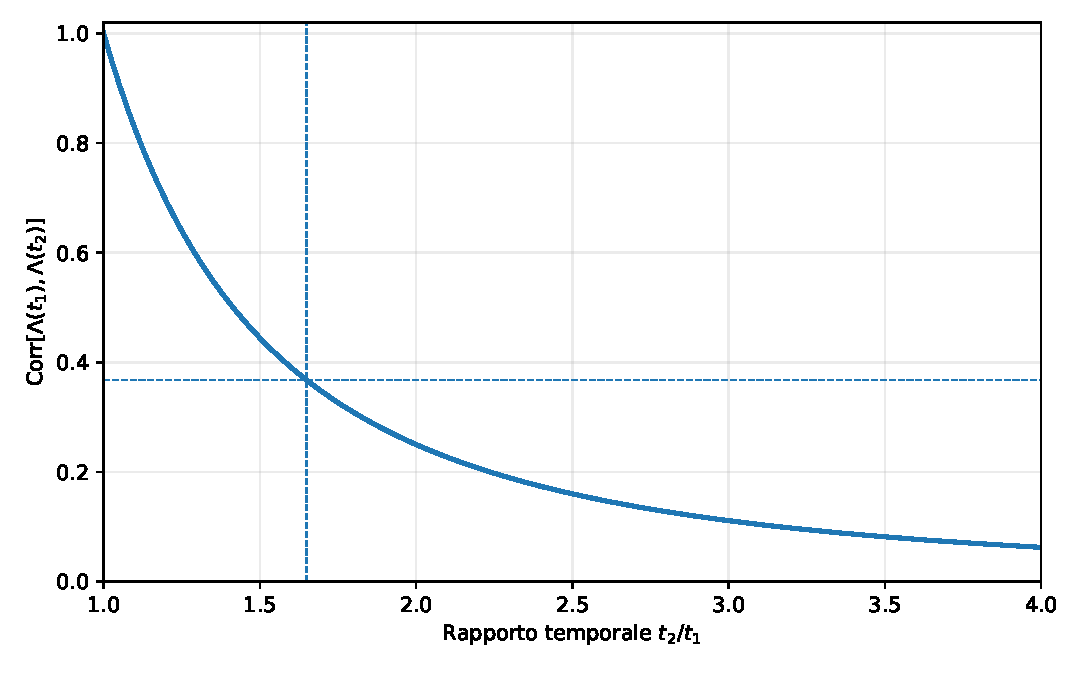
\includegraphics[width=0.72\textwidth]{r12g_temporal_nested.pdf}
 \caption{Correlazione temporale normalizzata del toy a coni annidati. In qualunque esatta era di potenza $V_4\propto t^4$, dunque $\mathcal C=(t_1/t_2)^2$. La linea tratteggiata indica $e^{-1}$.}
 \label{fig:r12g_temporal}
\end{figure}

\subsection{Correlazione spaziale: benchmark esatto in Minkowski}

Per due eventi simultanei a tempo $T$ in Minkowski, separati da distanza $d$, i coni passati troncati dalla superficie $t=0$ hanno volume individuale
\begin{equation}
 V=\frac{\pi}{3}(cT)^4.
\end{equation}
A una slice intermedia i due coni intersecano due sfere di ugual raggio; integrando il volume della lente tridimensionale si ottiene, per $0\le d\le2cT$,
\begin{equation}
 V_\cap=\frac{\pi}{48}(2cT-d)^3(2cT+d).
\end{equation}
Ponendo $x=d/(cT)$,
\begin{equation}
 \boxed{
 \mathcal C_{\rm Mink}(x)=
 1-x+\frac{x^3}{4}-\frac{x^4}{16},
 \qquad 0\le x\le2,
 }
 \label{eq:r12g_mink_kernel}
\end{equation}
mentre $\mathcal C=0$ per $x\ge2$. Il supporto compatto e causale: due eventi i cui coni passati non condividono elementi non sono correlati in questo toy.

In FLRW piatto, per due eventi simultanei separati da coordinata comovente $\chi$, il risultato si generalizza senza imporre omogeneita della realizzazione. Definendo
\begin{equation}
 r(t';t)=\int_{t'}^t\frac{c\,dt''}{a(t'')},
\end{equation}
e il volume di intersezione di due sfere comoventi uguali,
\begin{equation}
 v_\cap(r,\chi)=
 \frac{\pi}{12}(4r+\chi)(2r-\chi)^2\,\Theta(2r-\chi),
\end{equation}
si ha
\begin{equation}
 \boxed{
 V_\cap(t,\chi)=c\int_0^t dt'\,a^3(t')\,v_\cap[r(t';t),\chi].
 }
 \label{eq:r12g_flrw_overlap}
\end{equation}
La figura~\ref{fig:r12g_spatial} mostra il kernel normalizzato in un benchmark statico, radiativo e materiale, usando la separazione finale in unita del particle horizon. Il punto a correlazione $1/2$ si trova a $d/R_p\simeq0.533$ in Minkowski, $0.276$ nell'era radiativa e $0.186$ nell'era materiale. L'espansione pesa maggiormente le slice tardive, per le quali l'area comune dei coni e piccola, accelerando la decorrelazione spaziale in unita di $R_p$.

\begin{figure}[htbp]
 \centering
 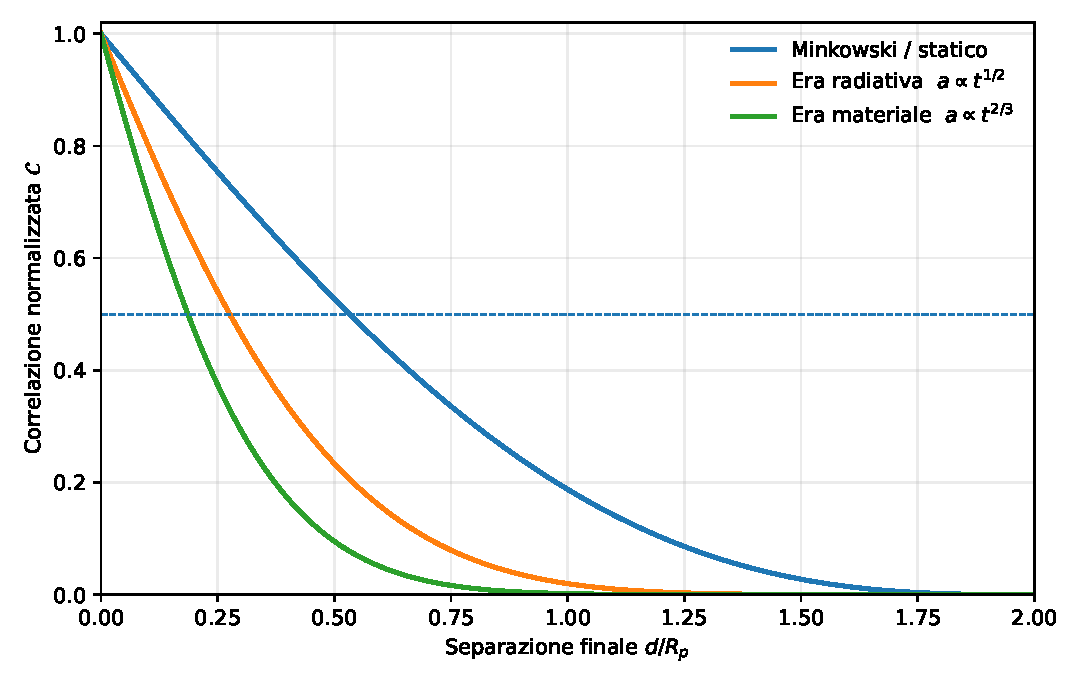
\includegraphics[width=0.76\textwidth]{r12g_spatial_overlap.pdf}
 \caption{Kernel spaziale del toy a sovrapposizione causale per eventi simultanei. Le curve FLRW sono ottenute integrando Eq.~\eqref{eq:r12g_flrw_overlap} per ere di potenza normalizzate al tempo finale.}
 \label{fig:r12g_spatial}
\end{figure}

\subsection{Il vantaggio e anche il problema: l'omogeneita non e piu imposta}

La costruzione di Eq.~\eqref{eq:r12g_overlap_kernel} evita di assegnare lo stesso valore di $\Lambda$ a tutta una slice FLRW: eventi diversi ricevono realizzazioni diverse ma correlate attraverso il proprio passato condiviso. Questo rende esplicita la non-localita causale richiesta dall'idea di base. Al tempo stesso produce inevitabilmente perturbazioni spaziali in ogni singola realizzazione. In letteratura, la prima implementazione cosmologica assunse invece omogeneita spaziale per ridurre il problema a un random walk temporale; lavori successivi hanno sottolineato che una teoria completa dovrebbe incorporare le inhomogeneita in modo non ad hoc e rispettare il carattere nonlocale delle fluttuazioni \cite{AhmedEtAl2004,AhmedSorkin2012,ZwaneAfshordiSorkin2017}.

Il kernel di overlap mostra anche perche il limite estremo di ``patch indipendenti'' e troppo semplice: due regioni possono essere fortemente correlate se i loro coni causali condividono una frazione significativa di quattro-volume. Questo non elimina i vincoli CMB. Analisi recenti di Model 1 trovano che le fluttuazioni tipiche danno fit CMB peggiori di $\Lambda$CDM e che le realizzazioni preferite richiedono variazioni piu piccole; una soppressione artificiale vicino alla last-scattering surface migliora il fit ma e precisamente il tipo di aggiustamento post hoc vietato nella presente roadmap \cite{DasNasiriYazdi2023}.

\subsection{Blocco di conservazione: una $\Lambda(x)$ locale non e una sorgente autonoma}

La difficolta piu severa non e statistica ma geometrica. Se si inserisce direttamente una realizzazione locale nella forma classica
\begin{equation}
 G_{\mu\nu}+\Lambda(x)g_{\mu\nu}=8\pi G T_{\mu\nu},
 \label{eq:r12g_local_lambda_einstein}
\end{equation}
l'identita di Bianchi implica
\begin{equation}
 \boxed{
 \partial_\nu\Lambda=8\pi G\,\nabla^\mu T_{\mu\nu}.
 }
 \label{eq:r12g_bianchi_exchange}
\end{equation}
Se la materia ordinaria e separatamente conservata, $\nabla^\mu T_{\mu\nu}=0$, allora $\partial_\nu\Lambda=0$: la realizzazione deve essere costante. Questo problema era gia esplicito nella formulazione originale di Everpresent $\Lambda$: una $\Lambda$ variabile richiede una modifica delle equazioni classiche o una interpretazione efficace diversa \cite{AhmedEtAl2004,AhmedSorkin2012}.

Si puo formalmente introdurre un tensore compensatore $X_{\mu\nu}$,
\begin{equation}
 G_{\mu\nu}+\Lambda(x)g_{\mu\nu}+X_{\mu\nu}=8\pi G T_{\mu\nu},
\end{equation}
con
\begin{equation}
 \nabla^\mu X_{\mu\nu}=-\partial_\nu\Lambda,
 \label{eq:r12g_compensator}
\end{equation}
oppure trasferire il flusso a un settore di materia efficace. Ma Eq.~\eqref{eq:r12g_compensator} non seleziona univocamente $X_{\mu\nu}$: una proiezione trasversa, un campo addizionale, una dinamica unimodulare quantistica o un completamento nonlocale sono teorie differenti. Sceglierne una equivale a introdurre nuova fisica, non a derivarla dal solo overlap causale.

Le implementazioni fenomenologiche esistenti confermano questa difficolta da angoli diversi: alcune scelgono una delle equazioni di Friedmann come guida stocastica, altre modellano le perturbazioni come un fluido/quintessenza covariante una volta fissata la storia omogenea \cite{AhmedSorkin2012,ZwaneAfshordiSorkin2017}. Queste procedure sono utili per i test osservativi, ma non costituiscono ancora la legge microscopica richiesta dal presente gate.

\subsection{Verdetto del Gate R12g}

R12g produce un progresso reale ma parziale. La geometria del passato condiviso seleziona un kernel di correlazione spazio-temporale non banale e, nel toy cumulativo, elimina la necessita di imporre un tempo di correlazione o una omogeneita perfetta a mano. Non seleziona pero in modo definitivo l'ampiezza microscopica, e soprattutto non fornisce il tensore conservato con cui una realizzazione locale possa gravitare.

\textbf{Gate R12g:} \status{CAUSAL-PAST OVERLAP DERIVES A NONTRIVIAL CORRELATION KERNEL, BUT THE AMPLITUDE AND A CONSERVED COVARIANT SOURCE LAW ARE NOT SELECTED; UNIQUE STOCHASTIC CLOSURE NOT DERIVED}.



\section{Gate R12h: completamento stocastico conservato}

R12g ha prodotto un campo scalare stocastico con correlazioni geometriche non arbitrarie, ma ha lasciato il vincolo
\begin{equation}
 \nabla^\mu X_{\mu\nu}=-\partial_\nu\Lambda
 \label{eq:r12h_compensator}
\end{equation}
per qualunque tensore compensatore aggiunto a $\Lambda(x)g_{\mu\nu}$. R12h chiede se causalita, Bianchi e la prescrizione retarded selezionino un completamento unico. Il risultato e negativo, ma il gate restringe fortemente la classe di possibilita.

\subsection{Lemma di non-unicita da Bianchi}

Supponiamo che $X^{(0)}_{\mu\nu}$ soddisfi Eq.~\eqref{eq:r12h_compensator}. Per qualunque tensore simmetrico $Y_{\mu\nu}$ separatamente conservato,
\begin{equation}
 \nabla^\mu Y_{\mu\nu}=0,
\end{equation}
anche
\begin{equation}
 X_{\mu\nu}=X^{(0)}_{\mu\nu}+Y_{\mu\nu}
\end{equation}
soddisfa lo stesso vincolo. La conservazione definisce quindi una classe affine di completamenti, non un singolo tensore. Causalita o minimalita possono restringere la classe, ma la parola ``minimo'' necessita a sua volta di un criterio fisico indipendente.

\subsection{Ramo A: proiezione trasversa retarded}

In spazio piatto esiste un benchmark particolarmente semplice. Definendo
\begin{equation}
 \mathcal P_{\mu\nu}[\Lambda]
 =\Lambda\eta_{\mu\nu}
 -\partial_\mu\partial_\nu\Box_{\rm ret}^{-1}\Lambda,
 \label{eq:r12h_flat_projector}
\end{equation}
si ha immediatamente
\begin{equation}
 \partial^\mu\mathcal P_{\mu\nu}
 =\partial_\nu\Lambda-
 \partial_\nu\Box\Box_{\rm ret}^{-1}\Lambda=0,
\end{equation}
una volta fissata la definizione retarded dell'inverso. Il prezzo e esplicito: la sorgente conservata e nonlocale.

La covariantizzazione ingenua con un solo scalare non basta. Se $U$ soddisfa $\Box U=\Lambda$,
\begin{equation}
 \nabla^\mu\left(\Lambda g_{\mu\nu}-\nabla_\mu\nabla_\nu U\right)
 =-R_{\nu}{}^{\alpha}\nabla_\alpha U,
 \label{eq:r12h_curvature_obstruction}
\end{equation}
quindi il termine di curvatura impedisce una semplice copia del proiettore piatto. Una costruzione covariante nota consiste invece nella decomposizione
\begin{equation}
 S_{\mu\nu}=S^{\rm T}_{\mu\nu}
 +\frac12\left(\nabla_\mu S_\nu+\nabla_\nu S_\mu\right),
 \qquad \nabla^\mu S^{\rm T}_{\mu\nu}=0,
 \label{eq:r12h_tensor_transverse}
\end{equation}
risolvendo per il vettore ausiliario tramite un operatore differenziale e una Green function. Modelli di gravita nonlocale usano precisamente estrazioni trasverse di questo tipo e definiscono gli inversi con Green function retarded per mantenere la causalita a livello di equazioni efficaci \cite{KehagiasMaggiore2014,MaggioreMancarella2014}.

Questo ramo dimostra \emph{esistenza}, non unicita. Occorre specificare almeno la Green function, la superficie iniziale/boundary conditions e le eventuali soluzioni omogenee; inoltre si puo sempre aggiungere un tensore conservato ulteriore. La proiezione trasversa retarded e quindi una chiusura covariante possibile, ma costituisce nuova struttura dinamica non contenuta nel solo kernel di overlap.

\subsection{Ramo B: conservare separatamente la materia modificando lo stress efficace}

Poniamo
\begin{equation}
 \rho_s(t)=\frac{\Lambda(t)}{8\pi G}
\end{equation}
e chiediamo che il settore stocastico sia un fluido isotropo separatamente conservato, mentre materia e radiazione seguono le loro equazioni standard. Allora
\begin{equation}
 \dot\rho_s+3H(\rho_s+p_s)=0
\end{equation}
impone univocamente, al solo livello FLRW omogeneo,
\begin{equation}
 \boxed{p_s=-\rho_s-\frac{\dot\rho_s}{3H}.}
 \label{eq:r12h_effective_pressure}
\end{equation}
Questa stessa reinterpretazione compare nelle discussioni fenomenologiche di un termine cosmologico variabile \cite{AhmedSorkin2012,ZwaneAfshordiSorkin2017}. Per $\dot\rho_s\neq0$ non si tratta piu di vuoto con $p=-\rho$; inoltre $w_s=p_s/\rho_s$ diverge ai passaggi per $\rho_s=0$, anche se $p_s$ puo restare finito.

Eq.~\eqref{eq:r12h_effective_pressure} chiude il background una volta assegnata la storia $\rho_s(t)$, ma non fornisce una estensione tensoriale unica in presenza di fluttuazioni spaziali: occorrono velocita, pressione non adiabatica, sound speed ed eventualmente anisotropic stress. Il completamento e quindi unico solo nel problema omogeneo ridotto, non come teoria covariante completa.

\subsection{Ramo C: preservare un vero vuoto e trasferire energia--momento}

Se si insiste invece su
\begin{equation}
 T_{\rm vac}^{\mu\nu}=-\rho_s(x)g^{\mu\nu},
 \end{equation}
allora
\begin{equation}
 \nabla_\mu T_{\rm vac}^{\mu\nu}=-\nabla^\nu\rho_s.
\end{equation}
La conservazione totale forza quindi
\begin{equation}
 \boxed{
 \sum_i Q_i^{\nu}=\nabla^\nu\rho_s,
 \qquad
 \nabla_\mu T_i^{\mu\nu}=Q_i^{\nu}.
 }
 \label{eq:r12h_interacting_vacuum}
\end{equation}
In FLRW omogeneo,
\begin{equation}
 \boxed{
 \sum_i\left[\dot\rho_i+3H(\rho_i+p_i)\right]
 =-\dot\rho_s.
 }
 \label{eq:r12h_background_exchange}
\end{equation}
Quindi, una volta assegnata $\rho_s(t)$, Bianchi fissa il \emph{trasferimento totale}. Questo e un risultato piu forte del semplice ``$Q$ arbitrario''. Tuttavia non stabilisce quale specie riceva il trasferimento, ne come esso si decomponga in energia e impulso rispetto ai diversi quattro-vettori di velocita. La teoria covariante dell'interacting vacuum conferma che un vuoto inhomogeneo deve interagire e che occorre una prescrizione covariante per l'energia di vuoto o, equivalentemente, per il transfer four-vector \cite{WandsDeSantiagoWang2012}.

Si ottengono quindi almeno due chiusure senza un nuovo coefficiente di background ma fisicamente inequivalenti: Eq.~\eqref{eq:r12h_effective_pressure} mantiene la materia separatamente conservata modificando lo stress del settore stocastico; Eq.~\eqref{eq:r12h_interacting_vacuum} mantiene $p_{\rm vac}=-\rho_{\rm vac}$ e forza uno scambio con gli altri settori.

\subsection{Il ramo unimodulare non elimina il problema}

Le equazioni unimodulari senza traccia possono essere scritte come
\begin{equation}
 R_{\mu\nu}-\frac14Rg_{\mu\nu}
 =8\pi G\left(T_{\mu\nu}-\frac14Tg_{\mu\nu}\right).
\end{equation}
Prendendone la divergenza si ottiene
\begin{equation}
 \partial_\nu(R+8\pi GT)
 =32\pi G\,\nabla^\mu T_{\mu\nu}.
 \label{eq:r12h_unimodular_div}
\end{equation}
Se definiamo localmente $R+8\pi GT=4\Lambda_s(x)$, allora
\begin{equation}
 \boxed{
 \partial_\nu\Lambda_s
 =8\pi G\,\nabla^\mu T_{\mu\nu}.
 }
 \label{eq:r12h_unimodular_same_condition}
\end{equation}
Con materia conservata, $\Lambda_s$ torna a essere costante. Un funzionale stocastico del passato causale non aggira dunque Bianchi semplicemente chiamandosi ``unimodulare'': per diventare locale e variabile necessita ancora di scambio o di un completamento nonlocale/globale.

\subsection{Nuovo blocker dal kernel R12g: non differenziabilita del campo grezzo}

Il kernel di overlap di R12g contiene un'informazione ulteriore. Nel benchmark Minkowski a tempo uguale,
\begin{equation}
 \mathcal C(x)=1-x+\frac{x^3}{4}-\frac{x^4}{16},
 \qquad x=\frac{d}{cT}.
\end{equation}
Per una varianza locale $\sigma^2$, l'incremento spaziale soddisfa
\begin{equation}
 \mathrm{Var}[\Lambda(\mathbf x+\mathbf d)-\Lambda(\mathbf x)]
 =2\sigma^2[1-\mathcal C(x)]
 =2\sigma^2 x+O(x^3).
\end{equation}
Pertanto
\begin{equation}
 \mathrm{Var}\!\left[
 \frac{\Lambda(\mathbf x+\mathbf d)-\Lambda(\mathbf x)}{d}
 \right]
 \sim\frac{2\sigma^2}{cT\,d}
 \longrightarrow\infty
 \qquad(d\to0).
 \label{eq:r12h_spatial_nondiff}
\end{equation}
Il toy non possiede quindi una derivata spaziale in media quadratica.

La stessa conclusione vale temporalmente. Nelle ere di potenza, scrivendo $\mathrm{Var}\Lambda(t)=K/t^4$, i coni annidati danno
\begin{equation}
 \mathrm{Cov}[\Lambda(t),\Lambda(t+\delta t)]
 =\frac{K}{(t+\delta t)^4},
\end{equation}
e quindi
\begin{equation}
 \mathrm{Var}[\Lambda(t+\delta t)-\Lambda(t)]
 =K\left[t^{-4}-(t+\delta t)^{-4}\right]
 \simeq\frac{4K}{t^5}\delta t.
\end{equation}
Segue
\begin{equation}
 \mathrm{Var}\!\left[\frac{\Delta\Lambda}{\delta t}\right]
 \simeq\frac{4K}{t^5\delta t}\to\infty.
 \label{eq:r12h_temporal_nondiff}
\end{equation}
Il comportamento e analogo a un random walk/Brownian scaling: gli incrementi rms sono proporzionali alla radice dell'intervallo. Di conseguenza Eq.~\eqref{eq:r12h_interacting_vacuum}, se applicata al campo grezzo, contiene un transfer four-vector distribuzionale. Una descrizione continua classica richiede almeno coarse-graining, una prescrizione di stochastic calculus oppure un operatore nonlocale che integri il rumore.

\begin{figure}[htbp]
 \centering
 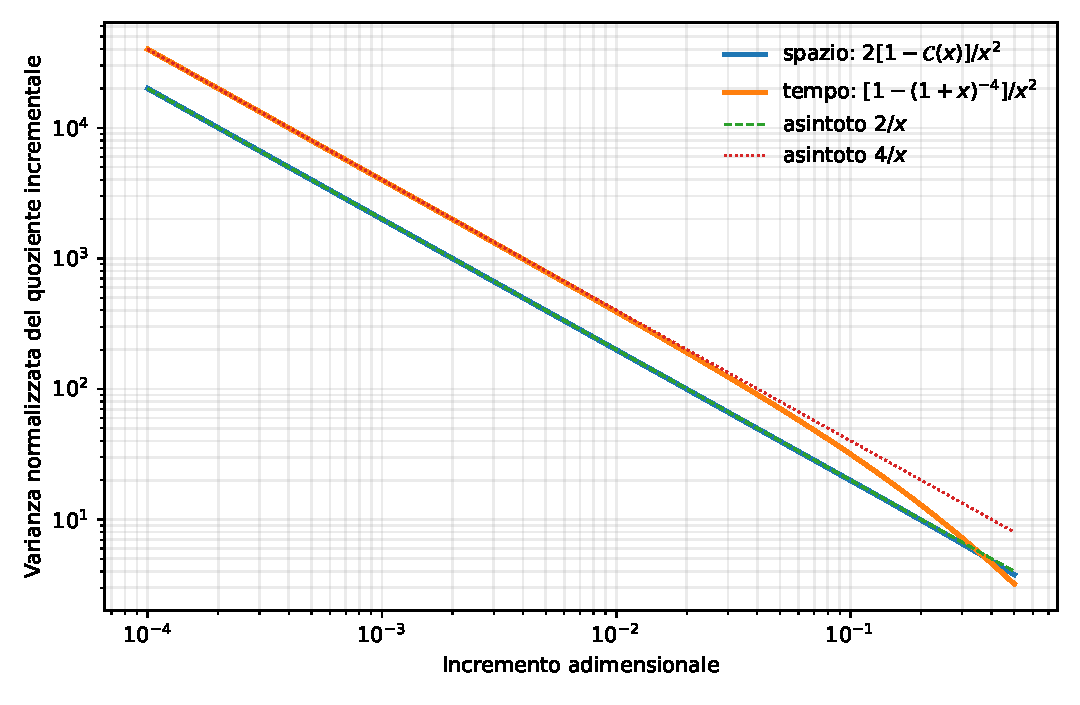
\includegraphics[width=0.74\textwidth]{r12h_nondifferentiability.pdf}
 \caption{Divergenza della varianza del quoziente incrementale nel toy di overlap. La cuspide lineare del kernel implica varianza della derivata che cresce come l'inverso dell'incremento sia nello spazio sia lungo la worldline. Le curve sono normalizzate alle varianze locali e alle scale $cT$ o $t$.}
 \label{fig:r12h_nondiff}
\end{figure}

Questo blocker non dimostra che una teoria discreta sia inconsistente: al livello fondamentale gli incrementi sono finiti e discreti. Dimostra pero che il limite continuo stocastico non puo essere inserito ingenuamente nelle equazioni classiche come una funzione differenziabile $\Lambda(x)$.

\subsection{Confronto con stochastic gravity}

La stochastic gravity fornisce un benchmark concettuale utile: nell'equazione Einstein--Langevin il rumore gravitazionale e un \emph{tensore} stocastico il cui noise kernel deriva dalle fluttuazioni del tensore energia--impulso, e la struttura di conservazione e incorporata nella costruzione \cite{HuVerdaguer2008}. Questo suggerisce che un completamento microscopico del nostro ramo causal-set dovrebbe probabilmente generare direttamente un oggetto tensoriale conservato, anziche prima generare uno scalare $\Lambda(x)$ e poi ripararlo a posteriori.

Non abbiamo pero derivato tale tensore dal causal set. La proiezione trasversa di R12h ne fornisce una possibile costruzione efficace, ma non e selezionata in modo unico dalla microstruttura di overlap.

\subsection{Verdetto del Gate R12h}

R12h stabilisce tre fatti distinti. Primo, un completamento conservato \emph{esiste}: si puo usare una proiezione trasversa retarded, un fluido efficace o uno scambio con la materia. Secondo, questi completamenti sono inequivalenti e Bianchi non ne seleziona uno. Terzo, il campo stocastico grezzo derivato dall'overlap non e differenziabile in media quadratica, quindi le chiusure locali che usano $\partial\Lambda$ richiedono una ulteriore prescrizione di coarse-graining o dinamica stocastica.

\textbf{Gate R12h:}
\begin{quote}\small\textsf{CONSERVATION CAN BE RESTORED IN MULTIPLE INEQUIVALENT WAYS; RETARDED TRANSVERSE COMPLETION EXISTS BUT REQUIRES NONLOCAL GREEN-FUNCTION/BOUNDARY DATA; INTERACTING-VACUUM AND EFFECTIVE-FLUID COMPLETIONS ARE DISTINCT; RAW OVERLAP NOISE IS NOT MEAN-SQUARE DIFFERENTIABLE; UNIQUE COVARIANT STOCHASTIC COMPLETION NOT DERIVED}.\end{quote}

\section{Gate R12i: rumore tensoriale causale conservato}

R12h ha mostrato che riparare a posteriori uno scalare stocastico $\Lambda(x)$ non seleziona un completamento unico. R12i cambia quindi l'oggetto fondamentale: si assume direttamente un tensore stocastico simmetrico $\Xi_{\mu\nu}$ con media nulla e conservazione covariante,
\begin{equation}
 \langle \Xi_{\mu\nu}(x)\rangle=0,
 \qquad
 \nabla^\mu\Xi_{\mu\nu}=0,
 \label{eq:r12i_source}
\end{equation}
e si chiede se il solo causal order, insieme al kernel di overlap di R12g, determini anche la struttura tensoriale del rumore.

Definiamo il noise bitensor
\begin{equation}
 N_{\mu\nu\rho'\sigma'}(x,y)
 =\left\langle\Xi_{\mu\nu}(x)\Xi_{\rho'\sigma'}(y)\right\rangle.
 \label{eq:r12i_noise_kernel}
\end{equation}
La conservazione richiede, distribuzionalmente,
\begin{equation}
 \boxed{
 \nabla_x^\mu N_{\mu\nu\rho'\sigma'}=0,
 \qquad
 \nabla_y^{\rho'}N_{\mu\nu\rho'\sigma'}=0.
 }
 \label{eq:r12i_noise_conservation}
\end{equation}
Questo e il tipo di struttura che compare nella stochastic gravity, dove il noise kernel e costruito dalle fluttuazioni del tensore energia--impulso quantistico ed e conservato in ciascun argomento per conseguenza della conservazione dell'operatore sorgente \cite{HuVerdaguer2008}.

\subsection{Decomposizione piatta: conservazione non significa unicita}

Nel benchmark di Minkowski, per un modo di Fourier non nullo con $k^2\neq0$, introduciamo
\begin{equation}
 \theta_{\mu\nu}=\eta_{\mu\nu}-\frac{k_\mu k_\nu}{k^2},
 \qquad
 k^\mu\theta_{\mu\nu}=0.
\end{equation}
I proiettori trasversi spin--2 e spin--0 per un tensore simmetrico sono \cite{Barnes1965}
\begin{align}
 P^{(2)}_{\mu\nu\rho\sigma}
 &=\frac12\left(\theta_{\mu\rho}\theta_{\nu\sigma}
 +\theta_{\mu\sigma}\theta_{\nu\rho}\right)
 -\frac13\theta_{\mu\nu}\theta_{\rho\sigma},\\
 P^{(0)}_{\mu\nu\rho\sigma}
 &=\frac13\theta_{\mu\nu}\theta_{\rho\sigma}.
 \label{eq:r12i_projectors}
\end{align}
Entrambi sono trasversi in ogni coppia di indici. In assenza di ulteriori vettori preferiti, un noise kernel simmetrico, parity-even e trasverso puo quindi contenere almeno
\begin{equation}
 \boxed{
 \widetilde N_{\mu\nu\rho\sigma}(k)
 =A(k)P^{(2)}_{\mu\nu\rho\sigma}
 +B(k)P^{(0)}_{\mu\nu\rho\sigma}.
 }
 \label{eq:r12i_spectral_general}
\end{equation}
La conservazione elimina i settori longitudinali ma non impone $A/B$. Anche se il kernel di overlap di R12g fornisse un unico inviluppo scalare $\widetilde C(k)$, resterebbe per esempio la famiglia
\begin{equation}
 A(k)=a(k)\widetilde C(k),
 \qquad
 B(k)=b(k)\widetilde C(k),
\end{equation}
con il rapporto $a/b$ non determinato dalla geometria del passato condiviso.

Un esempio minimo rende il punto esplicito. Dato uno scalare stocastico $\zeta$ con covarianza $C$, il campo
\begin{equation}
 \Xi^{(0)}_{\mu\nu}
 =\frac{1}{\sqrt3}\,\theta_{\mu\nu}\,\zeta
 \label{eq:r12i_spin0_source}
\end{equation}
e conservato e produce un noise kernel puramente spin--0, $N=C P^{(0)}$. Una sorgente trasversa-traceless indipendente puo invece produrre $N=C P^{(2)}$. Entrambe rispettano la stessa trasversalita e possono condividere lo stesso inviluppo scalare. Il solo overlap non contiene l'informazione necessaria per scegliere tra ``rumore di traccia'' e ``rumore di shear''.

\subsection{Toy di causal set marcato: fattorizzazione geometria--microfisica}

Il limite della sola geometria si vede direttamente generalizzando il toy di R12g. Supponiamo che ogni elemento causale $i$ porti un mark tensoriale casuale $J^{(i)}_{\mu\nu}$ con
\begin{equation}
 \langle J^{(i)}_{\mu\nu}\rangle=0,
 \qquad
 \left\langle
 J^{(i)}_{\mu\nu}J^{(j)}_{\rho\sigma}
 \right\rangle
 =\delta_{ij}\,\Sigma_{\mu\nu\rho\sigma}.
 \label{eq:r12i_marks}
\end{equation}
Definendo schematicamente
\begin{equation}
 \Xi_{\mu\nu}(x)
 =\frac{1}{N_x}\sum_{i\in P_x}J^{(i)}_{\mu\nu},
 \label{eq:r12i_marked_sum}
\end{equation}
si ottiene
\begin{equation}
 \boxed{
 \left\langle\Xi_{\mu\nu}(x)\Xi_{\rho\sigma}(y)\right\rangle
 =\frac{N_{xy}}{N_xN_y}\,\Sigma_{\mu\nu\rho\sigma},
 }
 \label{eq:r12i_factorized_cov}
\end{equation}
dove $N_{xy}$ conta gli elementi nel passato comune. Nel limite continuum $N_{xy}$ riproduce precisamente il fattore di volume di overlap che ha generato il kernel scalare di R12g.

La conseguenza e importante: il causal order determina il \emph{fattore geometrico} $N_{xy}/(N_xN_y)$, ma la ``polarizzazione'' tensoriale resta nella matrice microscopica $\Sigma_{\mu\nu\rho\sigma}$. Inoltre marks indipendenti non soddisfano automaticamente una legge di divergenza discreta: la conservazione richiede correlazioni fra marks, una dinamica o una proiezione ulteriore. Sostituire il mark tensoriale con il solo contributo scalare all'azione riporta invece al problema di R12g--R12h.

\subsection{In FLRW la liberta aumenta, non diminuisce}

In una cosmologia con quadrivelocita comovente $u^\mu$ e proiettore spaziale $h_{\mu\nu}=g_{\mu\nu}+u_\mu u_\nu$, qualunque sorgente simmetrica puo essere decomposta come
\begin{equation}
 \boxed{
 \Xi_{\mu\nu}
 =\delta\rho\,u_\mu u_\nu
 +\delta p\,h_{\mu\nu}
 +2u_{(\mu}q_{\nu)}
 +\pi_{\mu\nu},
 }
 \label{eq:r12i_flrw_decomp}
\end{equation}
con $q_\mu u^\mu=0$, $\pi_{\mu\nu}u^\nu=0$ e $\pi^\mu{}_{\mu}=0$. Le quattro equazioni $\nabla^\mu\Xi_{\mu\nu}=0$ collegano queste componenti, ma non determinano da sole pressione, flusso e anisotropic stress a partire dalla sola densita. In termini di perturbazioni scalari, vettoriali e tensoriali, occorrono quindi spettri e correlazioni incrociate addizionali.

Nel limite perfettamente omogeneo $q_\mu=\pi_{\mu\nu}=0$ e la conservazione riduce di nuovo al risultato di R12h,
\begin{equation}
 p_s=-\rho_s-\frac{\dot\rho_s}{3H},
\end{equation}
ma questa chiusura di background non specifica il noise kernel delle perturbazioni e non basta per CMB, lensing o crescita della struttura.

\subsection{Benchmark: perche stochastic gravity riesce dove l'overlap da solo non basta}

Nella stochastic gravity si definisce un noise kernel dal correlatore del vero operatore energia--impulso. La sua conservazione e la sua struttura tensoriale seguono dalla teoria quantistica della materia: propagatori, accoppiamenti, massa, stato quantistico e struttura dell'operatore $T_{\mu\nu}$ determinano il bitensore \cite{HuVerdaguer2008}. Questa e precisamente l'informazione che manca nel nostro toy di overlap.

Il causal set possiede gia costruzioni discrete per operatori scalari di d'Alembert e per estimatori della curvatura/azione \cite{BenincasaDowker2010,DowkerGlaser2013}. Tali risultati mostrano che order e number--volume correspondence possono codificare operatori geometrici non banali, ma non implicano automaticamente un noise bitensor energia--impulso unico con le proprieta di Eq.~\eqref{eq:r12i_noise_conservation}. Per il programma presente serve quindi un ulteriore passo microscopico: specificare quali gradi di liberta fluttuano e come la loro azione dipende dalla geometria.

\subsection{No-go ristretto di tensorizzazione overlap-only}

Sotto le ipotesi seguenti:
\begin{enumerate}[label=(\roman*)]
 \item l'unico input stocastico e il kernel scalare determinato dall'overlap dei passati causali;
 \item non si introducono marks tensoriali, nuovi campi o una azione microscopica addizionale;
 \item la sorgente gravitazionale richiesta e un tensore simmetrico non nullo e covariantemente conservato,
\end{enumerate}
la struttura tensoriale non e selezionata univocamente. La scelta algebraica locale $\Xi_{\mu\nu}\propto g_{\mu\nu}\zeta$ fallisce la conservazione per $\zeta$ variabile; una proiezione trasversa la ripristina ma introduce la scelta dell'operatore inverso e delle boundary conditions, mentre si possono sempre aggiungere settori trasversi ulteriori, incluso lo spin--2. Questo e il corrispettivo tensoriale del lemma di non-unicita di R12h.

\subsection{Verdetto del Gate R12i}

R12i restringe ulteriormente il problema. La geometria del passato causale puo determinare un inviluppo di correlazione non banale, ma non la polarizzazione tensoriale del rumore. La conservazione e una condizione necessaria e forte, tuttavia lascia almeno i settori trasversi spin--2 e spin--0 indipendenti nel benchmark piatto e piu funzioni in FLRW. La stochastic gravity mostra che una struttura tensoriale conservata emerge quando il rumore deriva da una microfisica con un vero tensore energia--impulso; order e volume da soli non forniscono ancora tale informazione.

\textbf{Gate R12i:}
\begin{quote}\small\textsf{CAUSAL OVERLAP FIXES A SCALAR CORRELATION ENVELOPE BUT NOT TENSOR POLARIZATION; CONSERVATION LEAVES INDEPENDENT TRANSVERSE SPIN--2/SPIN--0 SECTORS; A CONSERVED NOISE BITENSOR REQUIRES ADDITIONAL MICROPHYSICS OR A NONUNIQUE PROJECTION; UNIQUE TENSOR NOISE NOT DERIVED}.\end{quote}


\section{Gate R12j: azione stocastica causale e identita di Ward}

R12i ha mostrato che un noise bitensor conservato non e selezionato dal solo kernel scalare di overlap. Una possibilita piu strutturale e non scegliere direttamente $\Xi_{\mu\nu}$, ma farlo emergere dalla variazione metrica di una azione o effective action stocastica. In una teoria diffeomorphism-invariant la conservazione puo allora diventare una identita di Ward invece di una condizione imposta a posteriori. R12j verifica quanto questo meccanismo chiuda realmente il programma.

\subsection{Ward identity: cosa garantisce davvero}

Consideriamo una realizzazione microscopica $\omega$ descritta da una azione
\begin{equation}
 S_\omega[g,\phi^A],
\end{equation}
dove $\phi^A$ raccoglie eventuali gradi di liberta oltre alla metrica. Definiamo schematicamente la sorgente metrica
\begin{equation}
 \mathcal T^{\mu\nu}_\omega
 =\frac{2}{\sqrt{-g}}\frac{\delta S_\omega}{\delta g_{\mu\nu}}.
 \label{eq:r12j_metric_source}
\end{equation}
Per una trasformazione infinitesima generata da $\xi^\mu$,
\begin{equation}
 \delta_\xi g_{\mu\nu}=2\nabla_{(\mu}\xi_{\nu)},
 \qquad
 \delta_\xi\phi^A=\mathcal L_\xi\phi^A.
\end{equation}
L'invarianza di $S_\omega$ implica una Ward identity. Per un singolo scalare $\phi$ essa assume, a convenzioni di segno fissate dalla definizione di Eq.~\eqref{eq:r12j_metric_source}, la struttura
\begin{equation}
 \boxed{
 \nabla_\mu\mathcal T^{\mu}{}_{\nu}
 =\mathcal E_\phi\,\nabla_\nu\phi,
 }
 \qquad
 \mathcal E_\phi\equiv\frac{1}{\sqrt{-g}}\frac{\delta S}{\delta\phi}.
 \label{eq:r12j_ward_scalar}
\end{equation}
Quindi la sorgente metrica e automaticamente conservata quando i campi che trasformano sono anch'essi dinamici e soddisfano le loro equazioni, $\mathcal E_\phi=0$. L'identita non dice invece che un campo stocastico esterno, assegnato arbitrariamente nello spaziotempo, scompaia dalla divergenza.

Il benchmark piu semplice e precisamente la densita di vuoto variabile di R12g--R12h,
\begin{equation}
 S_\lambda=-\int d^4x\sqrt{-g}\,\lambda(x).
\end{equation}
Se $\lambda$ viene trattata come sorgente esterna, la variazione metrica produce
\begin{equation}
 T^{(\lambda)}_{\mu\nu}=-\lambda g_{\mu\nu},
 \qquad
 \boxed{\nabla^\mu T^{(\lambda)}_{\mu\nu}=-\partial_\nu\lambda}.
 \label{eq:r12j_external_lambda}
\end{equation}
Non vi e contraddizione con la diffeomorphism invariance del funzionale: la Ward identity contiene anche la variazione della sorgente esterna $\lambda$. Per ottenere un tensore separatamente conservato occorre quindi promuovere il rumore a gradi di liberta con dinamica propria, integrare tali gradi di liberta in una effective action consistente, oppure costruire una proiezione/nonlocalita come in R12h.

\subsection{Benchmark CTP: rumore e risposta nascono insieme}

La stochastic gravity mostra come questo possa accadere in una teoria efficace ben definita. Integrando campi quantistici di materia con il formalismo closed-time-path si ottiene una influence action; al secondo ordine nelle perturbazioni metriche, la sua parte immaginaria contiene il noise kernel, mentre la parte reale contiene la risposta dissipativa. Una trasformazione di Hubbard--Stratonovich riscrive la parte immaginaria come media su un tensore stocastico e conduce alla Einstein--Langevin equation \cite{HuMatacz1995,HuVerdaguer2008}.

Schematicamente,
\begin{equation}
 \operatorname{Im}S_{\rm IF}^{(2)}
 =\frac18\int d^4x\,d^4y\,
 h^-_{\mu\nu}(x)
 N^{\mu\nu\rho\sigma}(x,y)
 h^-_{\rho\sigma}(y),
 \label{eq:r12j_imag_if}
\end{equation}
e il tensore aleatorio equivalente soddisfa
\begin{equation}
 \langle\xi_{\mu\nu}(x)\rangle=0,
 \qquad
 \langle\xi_{\mu\nu}(x)\xi_{\rho\sigma}(y)\rangle=N_{\mu\nu\rho\sigma}(x,y).
\end{equation}
La conservazione di $N$ segue dalla Ward identity del vero operatore energia--impulso. Ma il valore del kernel non viene dalla simmetria: e calcolato dalla microfisica della materia e dal suo stato quantistico. La action route risolve quindi il problema di consistenza, non quello di selezione.

\subsection{Seconda variazione: Ward non seleziona spin--2 contro spin--0}

Il limite si vede gia al livello quadratico intorno a Minkowski. Dopo aver separato i settori di gauge, la parte fisica di una generica azione quadratica diffeomorphism-invariant puo essere scritta schematicamente come
\begin{equation}
 \boxed{
 \Gamma_{\rm phys}^{(2)}
 =\frac12\int_k h^{\mu\nu}(-k)
 \left[
 F_2(k^2)P^{(2)}_{\mu\nu\rho\sigma}
 +F_0(k^2)P^{(0)}_{\mu\nu\rho\sigma}
 \right]
 h^{\rho\sigma}(k).
 }
 \label{eq:r12j_quadratic_action}
\end{equation}
Poiche entrambi i proiettori sono trasversi,
\begin{equation}
 k^\mu P^{(2)}_{\mu\nu\rho\sigma}=0,
 \qquad
 k^\mu P^{(0)}_{\mu\nu\rho\sigma}=0,
\end{equation}
la Ward identity e soddisfatta per funzioni indipendenti $F_2$ e $F_0$. In forma covariante la stessa liberta compare, ad esempio, in effective actions con form factor distinti nei settori
\begin{equation}
 \int d^4x\sqrt{-g}\,
 \left[
 C_{\mu\nu\rho\sigma}F_2(\Box)C^{\mu\nu\rho\sigma}
 +R F_0(\Box)R+\cdots
 \right],
 \label{eq:r12j_covariant_formfactors}
\end{equation}
struttura standard delle espansioni quadratiche/nonlocali dell'effective action gravitazionale \cite{FranchinoVinas2019}. La simmetria controlla i settori ammessi ma non fissa il rapporto fra essi. Il no-go di R12i sopravvive quindi al passaggio a una azione.

\subsection{Azione causal-set: il primo cumulante non determina il secondo}

Il benchmark piu vicino alla microstruttura che stiamo esplorando e la famiglia Benincasa--Dowker--Glaser. Gli operatori discreti costruiti dall'ordine causale e dalla number--volume correspondence forniscono estimatori di $\Box$ e $R$ e quindi una azione puramente order-theoretic \cite{BenincasaDowker2010,DowkerGlaser2013}. La label invariance e la controparte discreta della general covariance nelle dinamiche causal-set \cite{RideoutSorkin2000}.

Per causal set ottenuti per sprinkling in regioni Lorentziane, il valore dell'azione e una variabile casuale. Il risultato oggi meglio controllato riguarda il primo cumulante:
\begin{equation}
 \boxed{
 \langle S_{\rm BDG}\rangle
 \longrightarrow
 S_{\rm EH}+S_{\rm joint}
 }
 \label{eq:r12j_bdg_mean}
\end{equation}
nel continuum limit, con un bulk Einstein--Hilbert e, su causal diamonds, un termine di bordo codimensione due \cite{MachetWang2021}.

Questo risultato e importante ma non determina
\begin{equation}
 \langle(S_{\rm BDG}-\langle S_{\rm BDG}\rangle)^2\rangle,
 \qquad
 \langle\delta_g S_{\rm BDG}(x)\,\delta_g S_{\rm BDG}(y)\rangle_c,
 \label{eq:r12j_second_cumulant}
\end{equation}
cioe precisamente i dati che servirebbero per costruire un noise kernel gravitazionale. Media e covarianza sono cumulanti indipendenti: conoscere il corretto limite classico dell'azione non seleziona automaticamente le fluttuazioni quantistiche/stocastiche attorno a quel limite.

C'e inoltre un problema gia noto a livello degli operatori causal-set: per le versioni piu locali le fluttuazioni da sprinkling possono essere molto grandi e crescere con la densita. Per smorzarle si introduce una scala fisica di nonlocalita $\xi$ maggiore della discreteness scale $\ell$; mantenendo $\xi$ fissata mentre $\ell\to0$, le fluttuazioni vengono mediate e possono diminuire \cite{DowkerGlaser2013}. Questo e utile tecnicamente, ma nel nostro programma significa che il settore stocastico richiede gia una mesoscale addizionale se non emerge da una dinamica piu fondamentale.

\begin{figure}[ht]
\centering
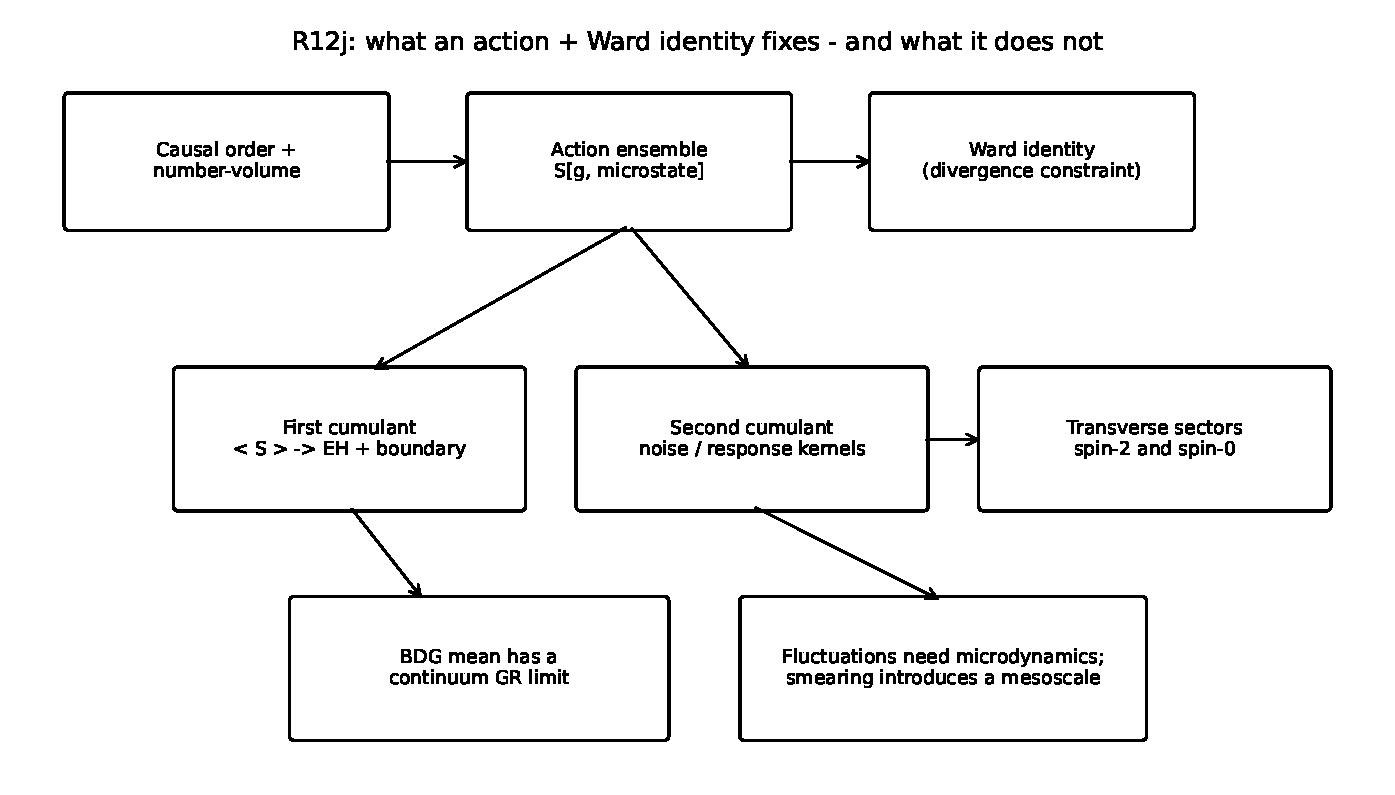
\includegraphics[width=0.94\textwidth]{r12j_action_ward_flow.pdf}
\caption{Schema del Gate R12j. Una azione covariante puo rendere la conservazione una Ward identity, ma il limite medio dell'azione e il suo secondo cumulante sono informazioni distinte. Nel benchmark causal-set il primo tende alla dinamica di Einstein, mentre il settore delle fluttuazioni richiede ancora microdinamica e, nelle costruzioni smeared note, una scala di nonlocalita.}
\label{fig:r12j_flow}
\end{figure}

\subsection{No-go ristretto: ``azione + Ward'' non e una chiusura}

Sotto le ipotesi:
\begin{enumerate}[label=(\roman*)]
 \item l'azione/effective action e diffeomorphism-invariant o label-invariant nel limite discreto appropriato;
 \item il suo primo cumulante riproduce Einstein--Hilbert nel continuum;
 \item non si specificano ulteriori gradi di liberta microscopici, measure quantistica, form factor, nonlocality scale o boundary data,
\end{enumerate}
non segue un noise bitensor unico. La Ward identity impone trasversalita quando tutte le variabili dinamiche sono on-shell, ma non determina il secondo cumulante, non fissa $F_2/F_0$ e non rende conservata una sorgente scalare esterna arbitraria. Il passaggio dall'azione classica media al rumore richiede quindi informazione dinamica che non e contenuta nella sola simmetria.

\subsection{Verdetto del Gate R12j}

R12j migliora il quadro ma non chiude il progetto. La via dell'azione e il modo piu pulito trovato finora per incorporare la conservazione: in una vera effective action la Ward identity rende trasversa la risposta stocastica coerente. Tuttavia la conservazione e solo una condizione strutturale. Il noise kernel vive nel secondo cumulante/parte immaginaria dell'effective action e dipende dalla microfisica; un campo casuale esterno non beneficia automaticamente della Ward identity. Le azioni causal-set mostrano inoltre che il corretto limite medio verso GR e compatibile con un settore di fluttuazioni ancora non controllato univocamente, e lo smearing conosciuto introduce una scala di nonlocalita.

\textbf{Gate R12j:}
\begin{quote}\small\textsf{DIFFEOMORPHISM/RELABELING INVARIANCE CAN MAKE CONSERVATION A WARD IDENTITY FOR DYNAMICAL ON-SHELL DEGREES OF FREEDOM, BUT DOES NOT CONSERVE AN ARBITRARY EXTERNAL STOCHASTIC SCALAR; THE SECOND CUMULANT/NOISE KERNEL IS NOT FIXED BY THE MEAN ACTION OR BY WARD IDENTITIES; BDG PROVIDES THE CORRECT CONTINUUM MEAN WHILE ITS FLUCTUATION SECTOR REQUIRES ADDITIONAL MICRODYNAMICS AND, IN SMEARED CONSTRUCTIONS, A NONLOCALITY SCALE; UNIQUE STOCHASTIC ACTION CLOSURE NOT DERIVED}.\end{quote}


\section{Gate R12k: secondo cumulante dell'azione causale e scala mesoscopica}

R12j ha separato con precisione il primo cumulante dell'azione dal suo settore stocastico. R12k rende quantitativo questo punto. Le domande sono tre: (i) quale crescita con il numero di elementi $N$ deve avere $\mathrm{Var}(S_{\rm BDG})$ per riprodurre una fluttuazione cosmologica di tipo Everpresent $\Lambda$? (ii) le costruzioni BDG note dimostrano gia tale scaling oppure forniscono soltanto il formalismo per calcolarlo? (iii) la scala di smearing/nonlocalita $\ell_k$ puo emergere da coarse-graining o rinormalizzazione anziche restare un parametro scelto a mano?

\subsection{La varianza BDG e ora un problema ben posto, ma non ancora risolto asintoticamente}

Moradi, Yazdi e Zilh\~ao hanno recentemente costruito un formalismo sistematico per le fluttuazioni delle quantita causal-set, con particolare attenzione all'azione BDG \cite{MoradiYazdiZilhao2025}. Indicando schematicamente con $C_i^{(d)}$ i coefficienti dell'operatore discreto e con $\mathcal K_{ij}$ le correlazioni tra conteggi di intervalli, la struttura della varianza puo essere scritta nella forma
\begin{equation}
 (\Delta S)^2
 =\langle S^2\rangle-\langle S\rangle^2
 =\frac{4}{\alpha_d^2}
 \sum_{i,j}C_i^{(d)}C_j^{(d)}\,\mathcal M_{ij},
 \label{eq:r12k_variance_matrix}
\end{equation}
con $\mathcal M_{ij}=\mathcal K_{ij}-\mathcal L_i\mathcal L_j$ nella convenzione del loro lavoro. Il risultato importante per il nostro programma non e un numero finale, ma il fatto che le correlazioni $\zeta$--$\zeta$, $\chi$--$\chi$ e $\zeta$--$\chi$ vengono ridotte a un insieme finito di integrali geometrici. In particolare, la varianza non puo essere ottenuta trattando i contributi dei diversi intervalli come indipendenti: gli overlap causali entrano in modo essenziale.

Tuttavia lo stesso lavoro dichiara esplicitamente che la valutazione delle fluttuazioni su specifici manifold --- iniziando da Minkowski e successivamente da FLRW --- e il passo successivo. Quindi, allo stato dell'arte considerato qui, non e ancora disponibile una legge generale verificata del tipo
\begin{equation}
 \mathrm{Var}(S_{\rm BDG})\sim A\,N^\gamma
 \label{eq:r12k_gamma_def}
\end{equation}
per il regime cosmologico che ci interessa. Questo impedisce di identificare automaticamente le fluttuazioni dell'azione con Everpresent $\Lambda$.

\subsection{Condizione di matching Everpresent: il secondo cumulante deve essere estensivo}

La condizione necessaria puo pero essere derivata senza conoscere i dettagli microscopici. In quattro dimensioni, il termine cosmologico nell'azione di Einstein--Hilbert scala schematicamente come
\begin{equation}
 S_\Lambda\sim -\frac{\Lambda V_4}{G},
\end{equation}
ignorando costanti numeriche che non influenzano gli esponenti. Una fluttuazione dell'azione produce quindi
\begin{equation}
 \Lambda_{\rm rms}\propto \frac{G}{V_4}\sqrt{\mathrm{Var}(S)}.
 \label{eq:r12k_lambda_from_S}
\end{equation}
Poniamo $N\propto V_4/\ell_{\rm cs}^{4}$ e assumiamo l'asintotica \eqref{eq:r12k_gamma_def}. A scala di discrezione fissata,
\begin{equation}
 \Lambda_{\rm rms}\propto N^{\gamma/2-1}.
 \label{eq:r12k_lambda_exponent}
\end{equation}
L'Everpresent scaling richiede invece
\begin{equation}
 \Lambda_{\rm rms}\propto V_4^{-1/2}\propto N^{-1/2}.
\end{equation}
Confrontando gli esponenti:
\begin{equation}
 \boxed{\gamma=1.}
 \label{eq:r12k_gamma_one}
\end{equation}
Quindi il requisito non e semplicemente ``l'azione deve fluttuare'': deve avere un secondo cumulante \emph{estensivo},
\begin{equation}
 \boxed{\mathrm{Var}(S_{\rm BDG})\propto N.}
 \label{eq:r12k_extensive_var}
\end{equation}
Se $\gamma<1$, la fluttuazione cosmologica decade piu rapidamente di $V_4^{-1/2}$; se $\gamma>1$, il rumore e superestensivo e non self-averaging; se $\gamma=2$, per esempio, $\Lambda_{\rm rms}$ tende addirittura a una costante in unita fissate dalla microfisica.

\begin{figure}[ht]
\centering
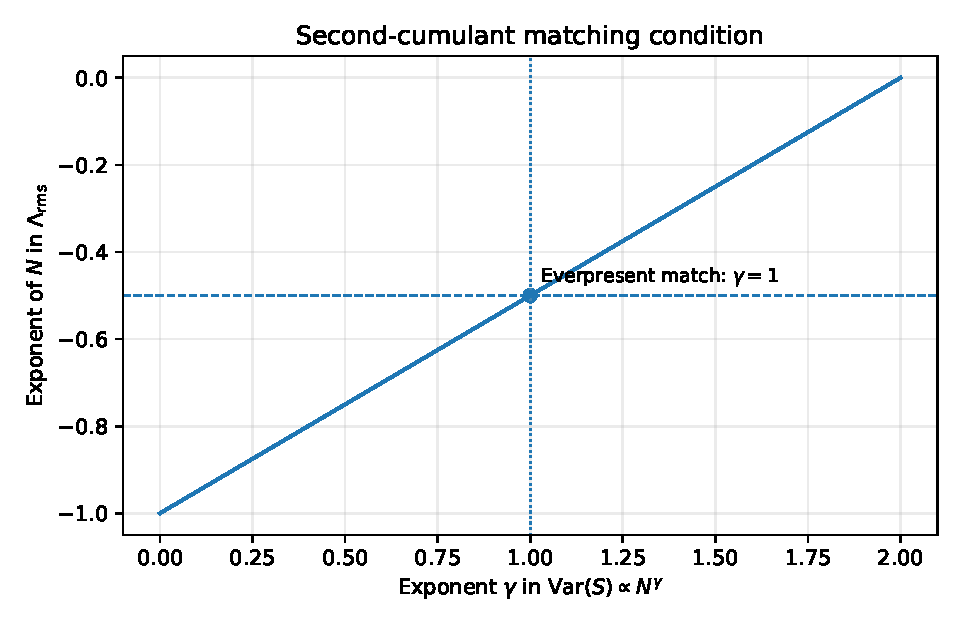
\includegraphics[width=0.76\textwidth]{r12k_second_cumulant_scaling.pdf}
\caption{Criterio di matching del secondo cumulante. Se $\mathrm{Var}(S)\propto N^\gamma$, allora $\Lambda_{\rm rms}\propto N^{\gamma/2-1}$. Il comportamento Everpresent $N^{-1/2}$ seleziona precisamente $\gamma=1$. Il grafico e una conseguenza algebrica del matching degli esponenti, non una misura numerica della varianza BDG.}
\label{fig:r12k_gamma}
\end{figure}

Questo risultato fornisce un gate quantitativo netto per il seguito: una futura simulazione o valutazione analitica della matrice \eqref{eq:r12k_variance_matrix} non dovra essere giudicata genericamente ``grande'' o ``piccola'', ma rispetto all'esponente $\gamma=1$.

\subsection{La scala mesoscopica nello smearing causal-set}

Le versioni nonlocali/smeared del d'Alembertiano causal-set introducono una scala fisica $\ell_k$ maggiore della discreteness scale $\ell$. In $d$ dimensioni viene comunemente usato il parametro
\begin{equation}
 \epsilon=\left(\frac{\ell}{\ell_k}\right)^d,
\end{equation}
che in quattro dimensioni diventa
\begin{equation}
 \epsilon=\left(\frac{\ell}{\ell_k}\right)^4.
 \label{eq:r12k_epsilon}
\end{equation}
Dowker e Glaser mostrano che l'averaging su piu layer puo sopprimere le grandi fluttuazioni del d'Alembertiano discreto; a $\ell_k$ fisico fissato, le fluttuazioni diminuiscono al diminuire di $\ell$ \cite{DowkerGlaser2013}. Anche le analisi dell'azione BDG sottolineano che questa scala di nonlocalita e un ingrediente fenomenologico utile a rendere controllabili le fluttuazioni \cite{Dowker2021Boundary,MoradiYazdiZilhao2025}.

Per visualizzare il problema, consideriamo soltanto come riferimento Poisson indipendente un blocco di volume $\ell_k^4$. Il numero medio di elementi nel blocco e
\begin{equation}
 n_k\sim\left(\frac{\ell_k}{\ell}\right)^4=\epsilon^{-1},
\end{equation}
e la sua fluttuazione relativa di conteggio sarebbe
\begin{equation}
 \frac{\sigma_{n_k}}{n_k}\sim n_k^{-1/2}
 =\sqrt{\epsilon}
 =\left(\frac{\ell}{\ell_k}\right)^2.
 \label{eq:r12k_poisson_block}
\end{equation}
Questa non e una formula per la varianza BDG --- le correlazioni tra intervalli possono modificarla profondamente --- ma e un benchmark minimale per capire i limiti di scala.

\begin{figure}[ht]
\centering
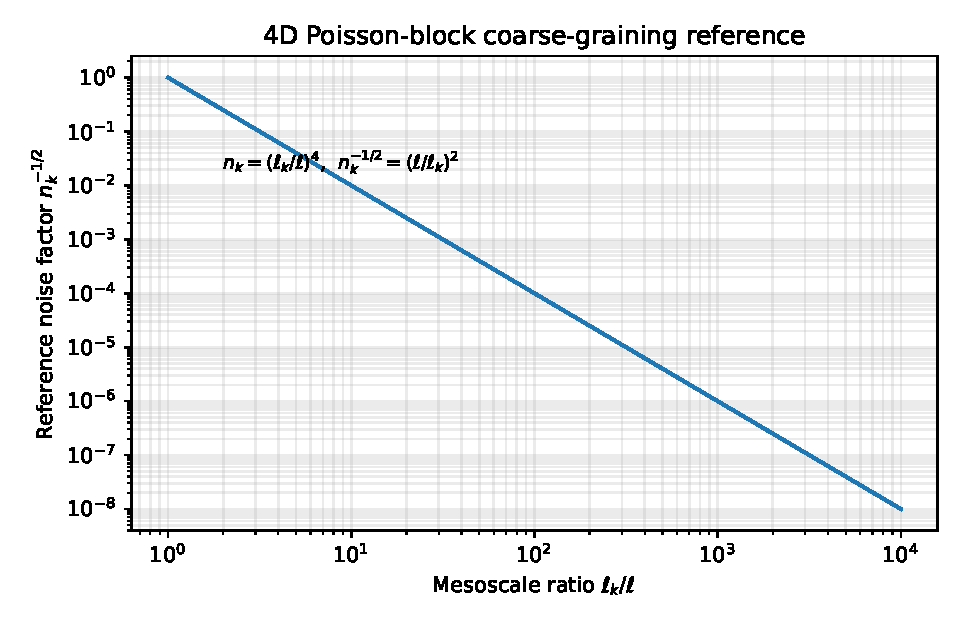
\includegraphics[width=0.76\textwidth]{r12k_mesoscale_suppression.pdf}
\caption{Riferimento di coarse-graining Poisson indipendente in $4D$: un blocco mesoscopico contiene $n_k=(\ell_k/\ell)^4$ elementi e la fluttuazione relativa di puro conteggio scala come $n_k^{-1/2}=(\ell/\ell_k)^2$. La curva non e una predizione della varianza BDG; serve a rendere esplicita la tensione tra soppressione del rumore e mantenimento di una sorgente stocastica finita.}
\label{fig:r12k_mesoscale}
\end{figure}

\subsection{Il trilemma del limite continuo}

Le scale note producono tre possibilita logicamente distinte.

\paragraph{A. $\ell_k$ fisica fissata mentre $\ell\to0$.}
Allora $\epsilon\to0$ e il numero di elementi nel volume di smearing diverge. Questo e precisamente il regime in cui lo smearing e progettato per far sparire le fluttuazioni da sprinkling e recuperare un operatore/azione deterministica nel limite continuo. E ottimo per ricostruire GR, ma non fornisce automaticamente un residuo stocastico cosmologico finito.

\paragraph{B. $\epsilon$ fissata mentre $\ell\to0$.}
In questo caso $\ell_k/\ell$ resta costante e quindi $\ell_k\to0$ insieme alla discreteness scale. Non emerge una mesoscale fisica macroscopia indipendente: il livello di coarse-graining resta agganciato all'UV.

\paragraph{C. Rumore fisico finito nel limite continuo.}
Per mantenere simultaneamente una scala fisica e un secondo cumulante non nullo e necessario che l'ampiezza stocastica subisca una rinormalizzazione o uno scaling anomalo. In altre parole, occorre una legge di running capace di compensare la soppressione statistica. Schematicamente, se
\begin{equation}
 \mathrm{Var}(S_{\ell,\ell_k})
 = Z_S(\ell,\ell_k)\,N^{\gamma(\ell,\ell_k)},
\end{equation}
una teoria Everpresent derivata dall'azione richiede che il flusso conduca a
\begin{equation}
 \gamma\to1,
 \qquad
 Z_S\to Z_*\ne0
\end{equation}
nel regime fisico rilevante. Questa e una condizione di punto fisso/critical scaling, non una conseguenza della sola Poisson sprinkling.

\subsection{Coarse-graining e RG: esiste il linguaggio, non ancora la selezione della mesoscale}

Un formalismo di coarse-graining per causal sets e stato effettivamente avviato: Eichhorn ha formulato una flow equation per una effective action causal-set usando il numero di elementi come parametro di scala \cite{Eichhorn2018}. Questo mostra che parlare di running dei couplings in un setting Lorentziano discreto non e soltanto analogia. Tuttavia non costituisce ancora una derivazione di una specifica $\ell_k$ o di un esponente $\gamma=1$ per la varianza BDG.

Una rassegna recente di Carlip e esplicita sullo stato del problema: un RG flow dei coefficienti BDG e una possibile strada per capire l'emergenza del continuum, ma non e ancora un programma sufficientemente sviluppato da selezionare una fixed-point action o una mesoscale fisica \cite{Carlip2024}. Pertanto non possiamo usare la parola ``rinormalizzazione'' come soluzione nominale: per il nostro gate servirebbe una traiettoria calcolata che selezioni simultaneamente (i) il corretto primo cumulante, (ii) $\gamma=1$ al secondo cumulante e (iii) una struttura tensoriale compatibile con R12i.

\subsection{Conseguenza per il rapporto spin--2/spin--0}

R12i aveva mostrato che un noise bitensor trasverso puo contenere
\begin{equation}
 \widetilde N=A(k)P^{(2)}+B(k)P^{(0)}.
\end{equation}
Il calcolo della sola varianza scalare dell'azione, anche se dimostrasse $\gamma=1$, non selezionerebbe automaticamente $A/B$. Per ottenere tale rapporto occorre il secondo funzionale rispetto al metrico, o equivalentemente una covarianza tensoriale dell'azione sotto perturbazioni geometriche. Quindi R12k fornisce una condizione necessaria sullo scaling del rumore, non chiude ancora il problema di polarizzazione.

\subsection{No-go ristretto di R12k}

Sotto le ipotesi:
\begin{enumerate}[label=(\roman*)]
 \item Poisson sprinkling con sola scala di discrezione $\ell$;
 \item azione BDG con corretto limite medio Einstein--Hilbert;
 \item eventuale smearing parametrizzato da una scala $\ell_k$ non ancora dinamicamente fissata;
 \item nessuna legge RG/microdinamica addizionale per il secondo cumulante,
\end{enumerate}
non segue ne un rumore cosmologico Everpresent, ne una mesoscale unica. Il matching Everpresent richiede $\mathrm{Var}(S)\propto N$, mentre il formalismo attuale delle fluttuazioni rende il calcolo ben posto ma non ne ha ancora stabilito l'asintotica su Minkowski/FLRW. Lo smearing controlla il rumore ma introduce $\ell_k$; nel limite continuo a $\ell_k$ fissata tende precisamente a sopprimere le fluttuazioni che vorremmo usare come sorgente fisica. Una sorgente stocastica finita richiede quindi una dinamica di rinormalizzazione del secondo cumulante, non soltanto un blocking cinematico.

\subsection{Verdetto del Gate R12k}

R12k restringe ulteriormente il progetto. Per la prima volta il settore stocastico possiede un criterio di accettazione quantitativo indipendente dai dati cosmologici: il secondo cumulante deve essere estensivo, $\gamma=1$. La letteratura recente ha costruito gli strumenti necessari per calcolare esattamente la varianza BDG includendo gli overlap tra intervalli, ma la valutazione asintotica specifica e ancora aperta. Le scale di nonlocalita note possono rendere il limite classico ben comportato, ma sono input e, a scala fisica fissata, spengono il rumore di sprinkling nel continuum. I programmi RG causal-set esistenti non hanno ancora selezionato una mesoscale o uno scaling critico del secondo cumulante.

\textbf{Gate R12k:}
\begin{quote}\small\textsf{EVERPRESENT MATCHING REQUIRES AN EXTENSIVE SECOND CUMULANT, VAR(S) PROPORTIONAL TO N; A GENERAL CORRELATION FORMALISM FOR THE BDG VARIANCE NOW EXISTS BUT ITS MINKOWSKI/FLRW ASYMPTOTIC SCALING IS NOT YET ESTABLISHED; SMEARING SUPPRESSES SPRINKLING FLUCTUATIONS AT FIXED PHYSICAL NONLOCALITY SCALE AND THEREFORE DOES NOT BY ITSELF LEAVE A FINITE STOCHASTIC CONTINUUM SOURCE; CAUSAL-SET COARSE-GRAINING/RG DOES NOT YET SELECT THE MESOSCALE OR THE REQUIRED GAMMA=1 FIXED-POINT SCALING; SECOND-CUMULANT CLOSURE NOT DERIVED}.\end{quote}


\section{Gate R12l: scaling quantistico del path sum e secondo cumulante}

R12k ha posto una condizione quantitativa semplice: se una fluttuazione cosmologica efficace viene estratta dal rapporto tra una fluttuazione dell'azione e il volume, lo scaling Everpresent richiede
\begin{equation}
\mathrm{Var}(S)\propto N^{\gamma},\qquad \gamma=1.
\label{eq:r12l_target_gamma}
\end{equation}
Fino a R12k, tuttavia, la media era quella cinematica delle Poisson sprinklings di uno stesso background. R12l distingue questa statistica dalla misura dinamica del path sum.

\subsection{Due ensemble diversi}

Per un background fissato $M$ si puo definire la media di sprinkling
\begin{equation}
\langle\mathcal O\rangle_{\rm spr}=\sum_{C\sim {\rm sprinkling}(M)}P(C|M)\,\mathcal O(C),
\end{equation}
mentre una dinamica causal-set assegna pesi alle geometrie stesse. Nel benchmark Lorentziano formale,
\begin{equation}
Z_N(g)=\sum_{C\in\Omega_N}\exp\!\left(\frac{i g}{\hbar}S[C]\right),
\end{equation}
con cumulanti connessi dell'azione generati da $\ln Z_N$. In particolare,
\begin{equation}
\kappa_2^{Q}(S)=-\hbar^2\frac{\partial^2\ln Z_N}{\partial g^2}.
\label{eq:r12l_quantum_cumulant}
\end{equation}
Dopo la continuazione analitica usata nelle simulazioni dei 2d-orders,
\begin{equation}
Z_E(\beta,N)=\sum_C e^{-\beta S[C]/\hbar},
\end{equation}
si ha invece
\begin{equation}
\mathrm{Var}_{\beta}(S)=\hbar^2\frac{\partial^2\ln Z_E}{\partial\beta^2},
\qquad
C=\frac{\beta^2}{\hbar^2}\mathrm{Var}_{\beta}(S).
\label{eq:r12l_heat_variance}
\end{equation}
Queste quantita non coincidono in generale con la varianza da sprinkling di R12k.

\subsection{Benchmark: finite-size scaling dei 2d-orders}

Il modello numerico meglio studiato usa i 2d-orders e l'azione Benincasa--Dowker. Il finite-size scaling mostra
\begin{equation}
\beta_c\propto N^{-1},\qquad \bar\beta\equiv\beta N=\mathcal O(1),
\end{equation}
una fase ad alta temperatura continuum-like e una fase a bassa temperatura cristallina, separate da una transizione di primo ordine \cite{GlaserOConnorSurya2018,Glaser2024Simulations}.

Lungo la traiettoria di scaling a $\bar\beta$ fissata, i risultati pubblicati implicano schematicamente
\begin{align}
\langle S\rangle_{\rm cont}&\sim N, & C_{\rm cont}&\sim N^0,\\
\langle S\rangle_{\rm crys}&\sim N^2, & C_{\rm crys}&\sim N^1.
\end{align}
Usando Eq.~\eqref{eq:r12l_heat_variance} e $\beta\sim N^{-1}$ segue quindi il benchmark
\begin{align}
\mathrm{Var}_{\beta}(S)_{\rm cont}&\sim N^2,\\
\mathrm{Var}_{\beta}(S)_{\rm crys}&\sim N^3.
\end{align}
Al punto di coesistenza di primo ordine il picco del calore specifico scala come $C_{\max}\sim N^2$; pertanto
\begin{equation}
\boxed{\mathrm{Var}_{\beta}(S)_{\rm coexist}\sim N^4.}
\label{eq:r12l_firstorder_var}
\end{equation}
Il meccanismo e trasparente: la distribuzione dell'azione diventa bimodale e la separazione tra le due medie domina il secondo cumulante.

\begin{figure}[htbp]
\centering
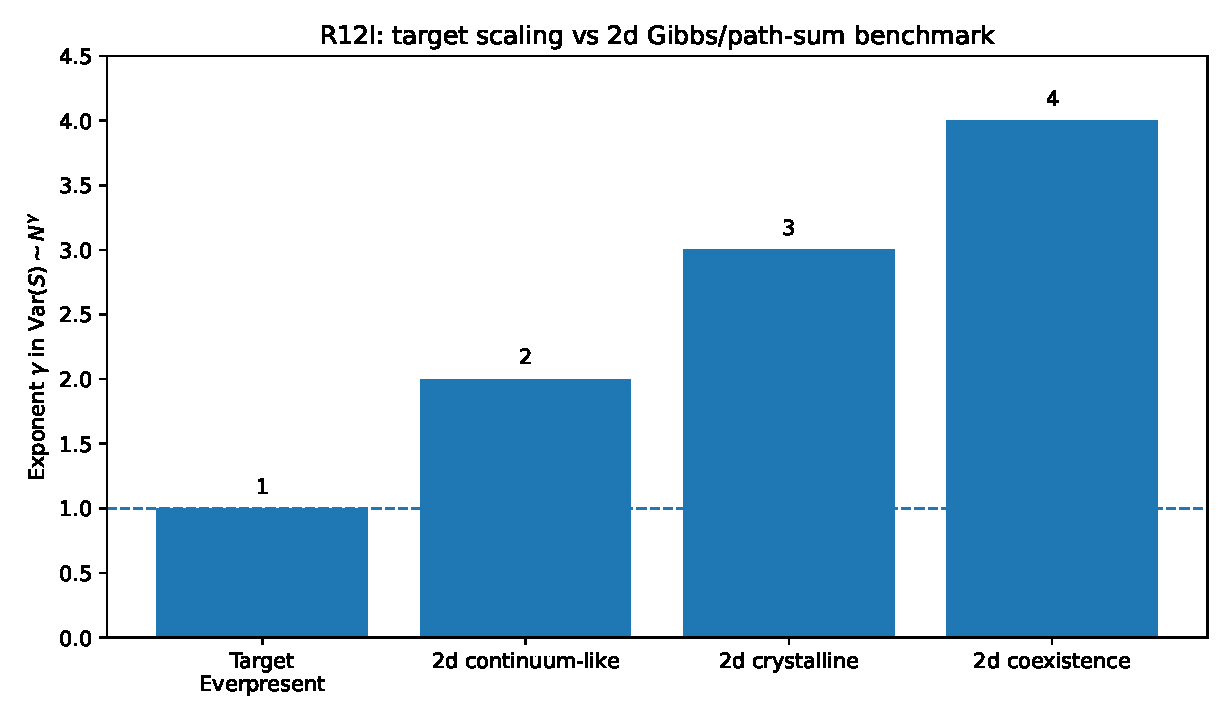
\includegraphics[width=0.78\linewidth]{r12l_pathsum_exponents.pdf}
\caption{Gate R12l. Confronto tra il requisito $\gamma=1$ di R12k e gli esponenti effettivi del benchmark termodinamico dei 2d-orders lungo $\bar\beta=\beta N$ fissato. Gli esponenti $2,3,4$ sono dedotti dal finite-size scaling pubblicato; non sono predizioni per il path sum Lorentziano 4d.}
\end{figure}

Questo benchmark non seleziona dunque Eq.~\eqref{eq:r12l_target_gamma}; anzi, le fluttuazioni dell'azione sono superestensive nei regimi considerati.

\subsection{Perche il risultato 2d non e un no-go 4d}

La conclusione precedente ha limiti precisi.
\begin{enumerate}
\item Il campionamento numerico usa una misura Gibbs con $\beta>0$ ottenuta per continuazione analitica; il valore quantistico e su un asse complesso e non esiste una dimostrazione che gli esponenti del secondo cumulante siano invarianti sotto tale continuazione.
\item Il sample space e ristretto ai 2d-orders. In due dimensioni la dinamica gravitazionale e speciale e non puo essere assunta rappresentativa del settore 4d cosmologico.
\item La transizione e di primo ordine. Non fornisce quindi il consueto fixed point critico con lunghezza di correlazione divergente che potrebbe selezionare una universalita del secondo cumulante.
\end{enumerate}
La review numerica moderna sottolinea proprio che il modello puro dei 2d-orders non mostra una transizione geometrica continua \cite{Glaser2024Simulations}.

\subsection{Il path sum Lorentziano fa comunque qualcosa di non banale}

Esistono risultati analitici direttamente Lorentziani: con l'azione causal-set Einstein--Hilbert/BDG ampie classi di causal set non-manifold-like, a partire dai two-level orders, possono essere soppresse per regioni del parametro di accoppiamento \cite{LoomisCarlip2018}. L'estensione combinatoria a classi layered piu generali rende plausibile che la dinamica possa contrastare l'enorme entropia dei causal set non-manifold-like; una review recente riassume questi progressi ma sottolinea che il settore sopravvissuto e l'eventuale flusso RG non sono ancora sufficientemente compresi \cite{Carlip2024}.

Questo e importante per il progetto: la misura $e^{iS}$ puo cambiare radicalmente quali geometrie dominano. Tuttavia le dimostrazioni di soppressione riguardano la dominanza del path sum, non il valore di $\kappa_2^{Q}(S)$ nel settore manifold-like e non mostrano
\begin{equation}
\kappa_2^{Q}(S)\propto N.
\end{equation}

\subsection{Connessione con il calcolo moderno della varianza BDG}

Il formalismo di Moradi, Yazdi e Zilh\~ao costruisce la matrice di correlazione necessaria a calcolare esattamente
\begin{equation}
\mathrm{Var}_{\rm spr}(S_{\rm BDG})
\end{equation}
per una Poisson sprinkling, ma non sostituisce il peso dinamico del path sum \cite{MoradiYazdiZilhao2025}. R12k e R12l sono quindi complementari:
\begin{equation}
\boxed{\text{R12k: }P(C|M)\quad\neq\quad\text{R12l: }e^{iS[C]/\hbar}.}
\end{equation}
Una teoria completa dovrebbe mostrare come il secondo oggetto rinormalizzi o sostituisca il primo e, in particolare, se il cumulante fisico finale diventi estensivo.

\subsection{No-go ristretto di R12l}

Dai risultati disponibili possiamo escludere la scorciatoia seguente:
\begin{quote}
``La sola presenza della nota transizione di fase BD nei 2d-orders seleziona automaticamente lo scaling Everpresent $\gamma=1$.''
\end{quote}
E falso nel benchmark termodinamico noto: lungo il finite-size scaling gli esponenti del secondo cumulante sono maggiori di uno, e la transizione e di primo ordine. Non possiamo invece escludere che un vero path sum Lorentziano 4d, una diversa fase manifold-like o un fixed point di una teoria piu completa producano $\gamma=1$.

\subsection{Verdetto del Gate R12l}

Il path sum e una distinzione fisica reale rispetto allo sprinkling e puo sopprimere intere famiglie di geometrie. Tuttavia, nei modelli numerici oggi controllati, la dinamica di fase non seleziona il secondo cumulante estensivo richiesto da R12k; nel settore Lorentziano piu vicino alla teoria fondamentale, tale cumulante non e ancora calcolato. Anche la struttura tensoriale spin--2/spin--0 resta non fissata.

\textbf{Gate R12l:}
\status{COMPLETATO -- KNOWN 2D PATH-SUM/GIBBS PHASE SCALING DOES NOT SELECT $\gamma=1$; FIRST-ORDER COEXISTENCE IS SUPEREXTENSIVE; LORENTZIAN BDG DYNAMICS CAN SUPPRESS NON-MANIFOLDLIKE CLASSES BUT ITS MANIFOLDLIKE QUANTUM SECOND CUMULANT IS NOT KNOWN; UNIQUE QUANTUM CLOSURE NOT DERIVED.}



\section{Gate R12m: protocollo preregistrato del secondo cumulante}

R12m trasforma il blocker teorico di R12k--R12l in un test numerico congelato \emph{prima} di osservare i risultati fisici. L'obiettivo non e misurare direttamente il vero path sum Lorentziano -- che soffre del problema di fase -- ma separare tre compiti: validare l'estimatore su un controllo con $\gamma=1$ noto, misurare lo scaling cinematico di sprinkling in un benchmark 2d, e misurare un benchmark Gibbs reale senza rinominarlo impropriamente $\gamma_Q$.

\subsection{Preregistrazione e separazione degli ensemble}

Il protocollo e stato congelato con SHA--256
\begin{quote}\ttfamily
1d93bf24d45d5a13781db2b91c0845272732fea300a809a27ff0d2c8e7050206
\end{quote}
prima dell'esecuzione del pilot. Sono stati fissati
\begin{equation}
\epsilon=0.21,
\qquad
N\in\{24,32,40,48,64,80,96\},
\end{equation}
insieme all'estimatore, al bootstrap e ai criteri di classificazione. I tre bracci sono:
\begin{enumerate}[label=(\roman*)]
\item \textbf{controllo sintetico}: $S_N=\sum_{i=1}^N\xi_i$ con $\xi_i\sim\mathcal N(0,1)$, dunque $\mathrm{Var}(S_N)=N$ e $\gamma=1$ esatto;
\item \textbf{sprinkling a $N$ fissato}: relative permutations indipendenti che rappresentano sprinklings condizionati a $N$ di un causal diamond 2d Minkowski, con azione BD a $\epsilon=0.21$;
\item \textbf{Gibbs continuum-like}: Metropolis su relative permutations con peso $\exp[-\beta S]$ e traiettoria preregistrata
\begin{equation}
\bar\beta\equiv\beta N=20,
\qquad
\beta=\frac{20}{N},
\end{equation}
scelta prima dei risultati e al di sotto del benchmark pubblicato della transizione dei 2d-orders per questo valore di $\epsilon$.
\end{enumerate}

Per ciascun braccio il fit primario e
\begin{equation}
\ln \widehat{\mathrm{Var}}_N(S)=a+\widehat\gamma\ln N.
\label{eq:r12m_fit}
\end{equation}
Il target preregistrato per l'estensivita e l'intervallo $0.8\le\gamma\le1.2$, con $R^2\ge0.95$. Per il braccio MCMC e richiesto inoltre $\mathrm{ESS}\ge200$ a ogni $N$. Le incertezze sono ottenute con 500 bootstrap; per l'MCMC viene usato un moving-block bootstrap con blocco determinato dall'autocorrelazione integrata.

\subsection{Amendment tecnico senza modifica statistica}

La prima esecuzione monolitica ha raggiunto il limite tecnico del singolo comando prima di produrre o salvare risultati fisici. Prima di ispezionare output e stato congelato un amendment puramente operativo, SHA--256
\begin{quote}\ttfamily
3dc2f33ccbf8a482e3cb33344ea207ccfb805e37b8eb399532565e31ee740d55
\end{quote}
che lascia invariati $N$, $\epsilon$, numero di campioni, $\bar\beta$, burn-in, thinning, estimatore, bootstrap e criteri PASS/FAIL. Le esecuzioni vengono soltanto suddivise per $N$ con substream RNG deterministici. Per $N=96$ il medesimo chain state e stato checkpointato ogni $10^4$ proposal fino ai $60000$ preregistrati; non sono stati ridotti ne burn-in ne numero di misure.

\subsection{Risultati preregistrati}

La tabella riporta il risultato del fit completo sulla griglia congelata.
\begin{table}[htbp]
\centering
\small
\begin{tabular}{lcccc}
\toprule
Braccio & $\widehat\gamma$ & CI 95\% & $R^2$ & Classificazione \\
\midrule
Controllo sintetico & 0.9930 & $[0.9777,1.0088]$ & 0.9998 & \status{SUPPORTS EXTENSIVE} \\
Sprinkling fixed-$N$ & 1.8574 & $[1.8401,1.8754]$ & 0.9952 & \status{REJECTS EXTENSIVE} \\
Gibbs continuum-like & 1.6368 & $[1.5657,1.7209]$ & 0.9906 & \status{REJECTS EXTENSIVE} \\
\bottomrule
\end{tabular}
\caption{Risultati del pilot R12m secondo il protocollo congelato. Il controllo sintetico verifica che la pipeline recuperi correttamente lo scaling estensivo. Il risultato Gibbs non e il cumulante del path sum Lorentziano.}
\label{tab:r12m_results}
\end{table}

Il controllo sintetico recupera quindi
\begin{equation}
\boxed{\widehat\gamma_{\rm ctrl}=0.99299}
\end{equation}
con intervallo che contiene il valore esatto $1$. La pipeline numerica non mostra dunque un bias macroscopico capace, da solo, di trasformare uno scaling estensivo in uno superestensivo.

Nel benchmark cinematico di sprinkling otteniamo invece
\begin{equation}
\boxed{\widehat\gamma_{\rm spr}=1.85736,
\qquad
95\%\ \mathrm{CI}=[1.84008,1.87544].}
\label{eq:r12m_gamma_spr}
\end{equation}
Sulla griglia congelata la varianza dell'azione BD cresce quindi sensibilmente piu rapidamente di $N$.

Nel benchmark Gibbs continuum-like:
\begin{equation}
\boxed{\widehat\gamma_{\rm G}=1.63678,
\qquad
95\%\ \mathrm{CI}=[1.56566,1.72086].}
\label{eq:r12m_gamma_gibbs}
\end{equation}
Il minimo effective sample size e $430.23$, superiore alla soglia preregistrata $200$. L'accettazione cresce da circa $0.63$ a $0.82$ lungo la griglia, mentre i tempi di autocorrelazione integrati delle serie gia thinnate restano circa tra $1.53$ e $2.32$.

\begin{figure}[htbp]
\centering
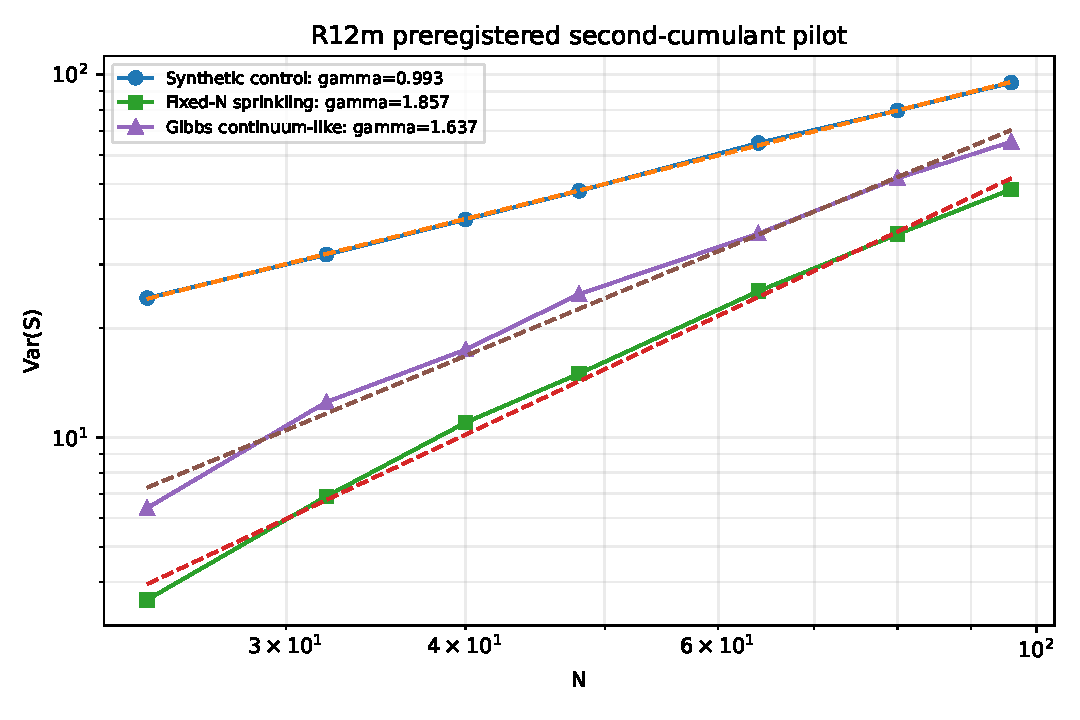
\includegraphics[width=0.82\linewidth]{r12m_variance_scaling.pdf}
\caption{Pilot R12m. Scaling della varianza dell'azione sulla griglia preregistrata. Il controllo sintetico segue $N^1$, mentre sprinkling e Gibbs mostrano esponenti superestensivi. Le linee tratteggiate sono i fit log--log congelati dal protocollo.}
\label{fig:r12m_scaling}
\end{figure}

\begin{figure}[htbp]
\centering
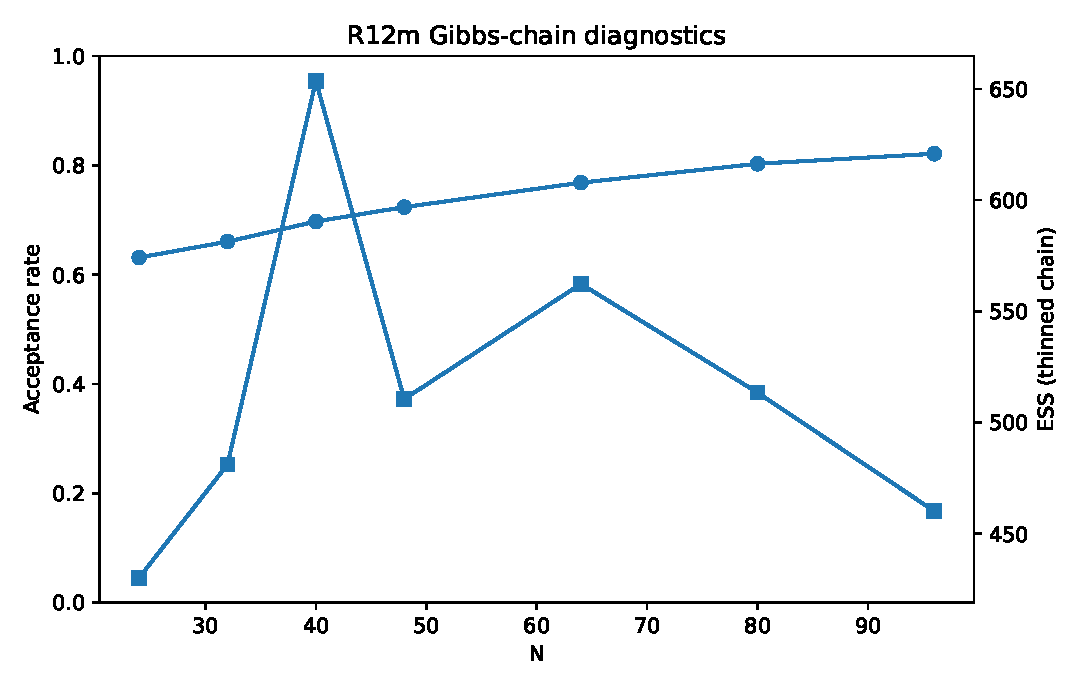
\includegraphics[width=0.75\linewidth]{r12m_gibbs_diagnostics.pdf}
\caption{Diagnostica del braccio Gibbs R12m. Acceptance rate ed effective sample size restano compatibili con i quality gate preregistrati sull'intera griglia.}
\label{fig:r12m_diag}
\end{figure}

\subsection{Cosa il pilot esclude e cosa non misura}

Il risultato consente un no-go ristretto e riproducibile:
\begin{quote}
per $\epsilon=0.21$, sulla griglia $24\le N\le96$, ne il benchmark cinematico fixed-$N$ ne il benchmark Gibbs continuum-like a $\bar\beta=20$ mostrano lo scaling estensivo richiesto da R12k; entrambi lo respingono secondo i criteri fissati prima del calcolo.
\end{quote}
Non segue invece
\begin{equation}
\gamma_Q\ne1.
\end{equation}
Il vero cumulante Lorentziano e definito dalla misura oscillante $e^{iS/\hbar}$, non dal peso reale $e^{-\beta S}$. Il pilot R12m non risolve il sign problem e non autorizza a sostituire $\gamma_{\rm G}$ a $\gamma_Q$. Inoltre il sample space e 2d e il range di $N$ e un pilot finite-size, non un limite 4d cosmologico.

\subsection{Verdetto del Gate R12m}

R12m raggiunge il proprio obiettivo metodologico: il protocollo e preregistrato, il controllo positivo recupera $\gamma=1$, i due benchmark fisici testati risultano superestensivi e il braccio MCMC supera i quality gate. Il blocker residuo e ora piu preciso: non serve un altro fit Gibbs, ma un accesso al cumulante connesso della misura Lorentziana o a una sua ricostruzione controllata tramite density of states / characteristic function.

\textbf{Gate R12m:}
\status{COMPLETATO -- PREREGISTERED PIPELINE VALIDATED; FIXED-N SPRINKLING GIVES $\gamma_{\rm spr}=1.8574$ AND THE CONTINUUM-LIKE GIBBS BENCHMARK GIVES $\gamma_{\rm G}=1.6368$, BOTH REJECTING THE FROZEN $\gamma=1$ TARGET BAND; THE SYNTHETIC CONTROL RECOVERS $\gamma=0.9930$; THE TRUE LORENTZIAN QUANTUM CUMULANT $\gamma_Q$ REMAINS UNMEASURED; NO COSMOLOGICAL CLOSURE AUTHORIZED.}


\section{Gate R12n: characteristic function e density of states Lorentziana esatta}

Il Gate R12m ha escluso l'uso del Gibbs reale come sostituto della misura oscillante. R12n affronta quindi direttamente il fattore di fase nel piu piccolo benchmark in cui e possibile una enumerazione completa. Prima di osservare i risultati e stato congelato il protocollo \texttt{PREREGISTRATION\_R12N.json}; un successivo timeout ha richiesto soltanto di dividere tecnicamente il calcolo ad alta precisione per $N=10$, senza modificare $N$, coupling, griglia o criteri di classificazione.

\subsection{Sample space e density of states esatta}

Si mantiene lo stesso benchmark dei 2d-orders usato nel pilot precedente. Il primo ordine totale viene fissato all'identita e ogni permutazione relativa $p\in S_N$ viene enumerata esattamente una volta. Questo produce un sample space di rappresentazioni/labelling controllato, non il quoziente completo per isomorfismi dei causal set non etichettati; tale differenza viene mantenuta esplicita nell'etichetta del risultato, $\gamma_Q^{\rm rep}$. Il ruolo dei 2d-orders come toy model di causal-set quantum gravity e ben noto \cite{BrightwellHensonSurya2008,GlaserOConnorSurya2018}.

Per ogni permutazione viene calcolato il vettore completo delle abbondanze degli intervalli
\begin{equation}
 \mathbf N(C)=(N_0,N_1,\ldots,N_{N-1})
\end{equation}
e la stessa azione BD del Gate R12m,
\begin{equation}
 S(C)=4\epsilon\left[N-2\epsilon\sum_{n=0}^{N-1}N_n f(n,\epsilon)\right],\qquad \epsilon=0.21.
\end{equation}
La density of states non viene bin-nata: configurazioni con lo stesso vettore $\mathbf N$ vengono raggruppate esattamente, conservandone la molteplicita. La costruzione e coerente con il fatto che l'azione discreta in 2d e determinata dalle abbondanze degli intervalli \cite{BenincasaDowkerSchmitzer2011}.

\begin{table}[htbp]
\centering
\caption{R12n: enumerazione esatta del benchmark representation-weighted. La somma delle molteplicita DOS e stata verificata uguale a $N!$ per ogni riga.}
\begin{tabular}{r r r r r}
\toprule
$N$ & permutazioni & stati DOS & $|\phi_N(1)|$ & $|\kappa_2(1)|$\\
\midrule
4  & 24      & 10    & 0.931609 & 0.149542\\
5  & 120     & 28    & 0.904147 & 0.211007\\
6  & 720     & 95    & 0.878631 & 0.264256\\
7  & 5040    & 369   & 0.854623 & 0.309417\\
8  & 40320   & 1750  & 0.830767 & 0.352043\\
9  & 362880  & 9566  & 0.805496 & 0.399928\\
10 & 3628800 & 60945 & 0.777482 & 0.459367\\
\bottomrule
\end{tabular}
\end{table}

\subsection{Characteristic function e cumulante connesso}

Il protocollo fissa $\hbar=1$ e definisce
\begin{equation}
 \phi_N(g)=\frac{1}{N!}\sum_C e^{igS_C},
\end{equation}
insieme alla media complessa
\begin{equation}
 \mu_N(g)=\frac{\sum_C S_C e^{igS_C}}{\sum_C e^{igS_C}}
\end{equation}
e al secondo cumulante connesso
\begin{equation}
 \kappa_{2,N}(g)=
 \frac{\sum_C S_C^2e^{igS_C}}{\sum_C e^{igS_C}}-\mu_N(g)^2
 =-\frac{d^2}{dg^2}\ln Z_N(g).
 \label{eq:r12n_kappa2}
\end{equation}
La quantita primaria preregistrata e
\begin{equation}
 K_N\equiv |\kappa_{2,N}(1)|.
\end{equation}
Le somme DOS sono state valutate con 80 cifre decimali; una implementazione double indipendente concorda con errore relativo massimo $2.3\times10^{-16}$ per $\phi$ e $1.4\times10^{-14}$ per $\kappa_2$.

\begin{figure}[htbp]
\centering
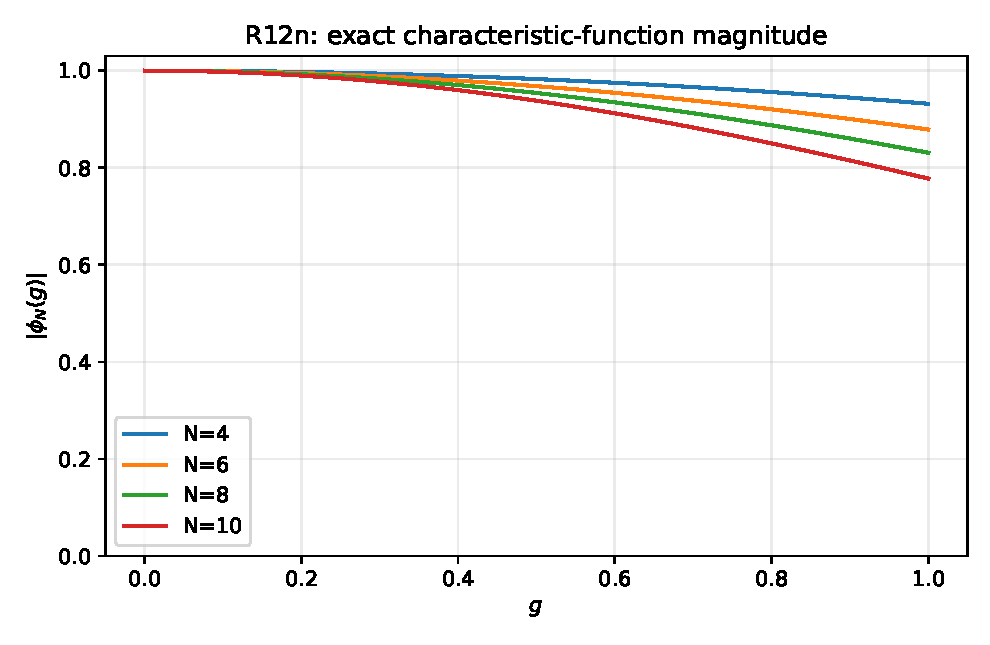
\includegraphics[width=0.74\textwidth]{r12n_characteristic_phase.pdf}
\caption{R12n. Modulo della characteristic function esatta sulla griglia preregistrata $g=0,0.05,\ldots,1$. Nel range testato non compare una cancellazione di fase severa: il minimo globale della griglia e il valore $N=10,g=1$, $|\phi|=0.77748$.}
\end{figure}

Il diagnostico preregistrato classifica il sign problem come \status{MILD}, poiche
\begin{equation}
 \min_N|\phi_N(1)|=0.7774817>10^{-2},
\end{equation}
e nessun punto attiva il guard $|\phi|<10^{-40}$. Il fatto che il problema di fase sia debole a queste taglie e un risultato del benchmark, non una garanzia per $N$ grandi.

\subsection{Scaling preregistrato}

Il fit primario congelato e
\begin{equation}
 \ln K_N=a+\gamma_Q^{\rm rep}\ln N,
\end{equation}
con tutti i valori $N=4,\ldots,10$. Si ottiene
\begin{equation}
 \boxed{\gamma_Q^{\rm rep}=1.180661},\qquad \boxed{R^2=0.993186}.
\end{equation}
I due controlli di stabilita preregistrati forniscono
\begin{align}
 \gamma_{4\ldots9}&=1.189321,\qquad R^2=0.990738,\\
 \gamma_{5\ldots10}&=1.092766,\qquad R^2=0.998029.
\end{align}
Entrambi restano nel support band $[0.7,1.3]$, mentre il fit completo cade nel target band $[0.8,1.2]$. Ne segue, senza modifiche post hoc,
\begin{equation}
 \boxed{\texttt{CONSISTENT\_WITH\_EXTENSIVE\_REP}.}
\end{equation}

\begin{figure}[htbp]
\centering
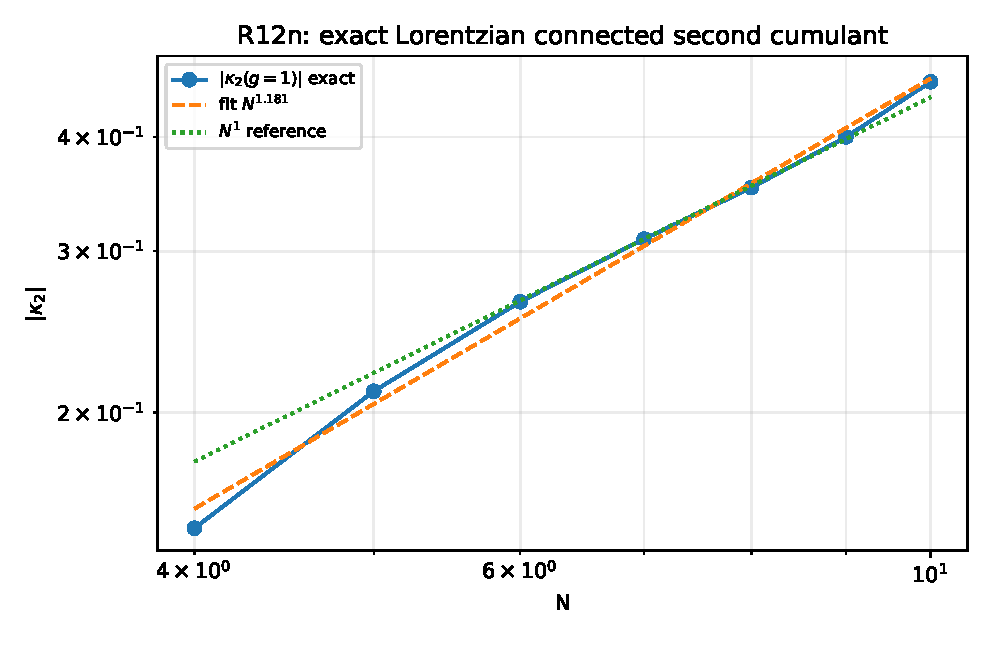
\includegraphics[width=0.74\textwidth]{r12n_lorentzian_scaling.pdf}
\caption{R12n. Scaling esatto di $|\kappa_2(g=1)|$ nel benchmark Lorentziano representation-weighted. La linea $N^1$ e solo un riferimento; il fit preregistrato usa tutti e sette i punti e restituisce $\gamma_Q^{\rm rep}=1.1807$.}
\end{figure}

Come controllo secondario, la varianza uniforme $g=0$ sulle sole taglie $N=4$--$10$ ha un esponente apparente $1.35275$, differente sia dal risultato Lorentziano sia dal valore $1.857$ misurato in R12m su $N=24$--$96$. Questo mostra direttamente quanto le stime finite-size dipendano dalla finestra di $N$ e rafforza il divieto di estrapolare il presente $\gamma_Q^{\rm rep}$ alla 4d.

\subsection{Cosa abbiamo e cosa non abbiamo ottenuto}

R12n e il primo test del progetto in cui la misura $e^{iS}$ viene sommata direttamente, senza analytic continuation a un peso reale. Il risultato e positivo rispetto al criterio di R12k: nel piccolo benchmark esatto il secondo cumulante Lorentziano e compatibile con una legge quasi estensiva. Inoltre le fasi modificano sostanzialmente lo scaling rispetto alla misura uniforme/Gibbs, quindi non era lecito inferire $\gamma_Q$ da R12m.

Tuttavia restano quattro limiti forti:
\begin{enumerate}
\item il massimo e $N=10$, molto lontano da un regime asintotico;
\item il sample space e 2d e representation-weighted;
\item il sign problem potrebbe emergere soltanto a taglie maggiori;
\item la magnitudine del cumulante non risolve ancora il problema tensoriale spin--0/spin--2 di R12i.
\end{enumerate}
Pertanto il risultato non sblocca R13.

\subsection{Verdetto del Gate R12n}

\textbf{Gate R12n:}
\begin{quote}
\status{EXACT LORENTZIAN SMALL-N REPRESENTATION BENCHMARK IS CONSISTENT WITH EXTENSIVE SECOND-CUMULANT SCALING: $\gamma_Q^{\rm rep}=1.1807$, $R^2=0.9932$, WITH MILD PHASE CANCELLATION THROUGH $N=10$. THIS IS NOT THE FULL UNLABELED OR 4D PATH SUM; ASYMPTOTIC $\gamma_Q$ AND TENSOR NOISE REMAIN UNRESOLVED.}

\end{quote}

\section{Gate R12o: estensione Monte Carlo Lorentziana e onset del sign problem}

R12n ha fornito una somma oscillante esatta soltanto fino a $N=10$. Il Gate R12o congela quindi, prima dei nuovi risultati, un protocollo di estensione che non modifica il coupling primario $g=1$ e non usa pesi Gibbs. Il file \texttt{PREREGISTRATION\_R12O.json} fissa sample space, griglia di $N$, numerosita, seed, bootstrap, quality gate e criteri di classificazione. Il principio metodologico e semplice: prima l'estimatore approssimato deve riprodurre la DOS esatta di R12n; soltanto dopo puo essere usato oltre la finestra enumerabile.

\subsection{Estimatore e preregistrazione}

Per ogni $N$ si estraggono $10^6$ permutazioni relative indipendenti e uniformi, suddivise in $20$ batch indipendenti da $50\,000$ configurazioni. Per ogni configurazione si calcola la stessa azione BD di R12n e, senza costruire un peso reale ausiliario, si stimano direttamente
\begin{align}
 \widehat\phi_N(g)&=\frac{1}{M}\sum_{j=1}^{M}e^{igS_j},\\
 \widehat m_{1,N}(g)&=\frac{1}{M}\sum_{j=1}^{M}S_j e^{igS_j},\\
 \widehat m_{2,N}(g)&=\frac{1}{M}\sum_{j=1}^{M}S_j^2 e^{igS_j},
\end{align}
con
\begin{equation}
 \widehat\kappa_{2,N}(g)=
 \frac{\widehat m_{2,N}(g)}{\widehat\phi_N(g)}-
 \left(\frac{\widehat m_{1,N}(g)}{\widehat\phi_N(g)}\right)^2.
 \label{eq:r12o_mc_kappa}
\end{equation}
Il protocollo vieta esplicitamente di cambiare $g=1$, aumentare selettivamente il numero di campioni dopo aver osservato cancellazioni, eliminare punti salvo il quality gate congelato, o sostituire il Lorentziano con il Gibbs.

La validazione primaria usa $N=8,9,10$ e richiede errore relativo complesso $<1\%$ su $\phi$ e $<8\%$ su $\kappa_2$ rispetto al risultato esatto. L'estensione e preregistrata su
\begin{equation}
 N=12,14,16,20,24,32,40,48,64.
\end{equation}
Ogni punto e ammesso allo scaling soltanto se l'average phase ha signal-to-noise ratio almeno $8$ e l'intervallo bootstrap 95\% di $|\kappa_2|$ ha semiampiezza relativa non superiore a $20\%$. Il fit primario richiede inoltre almeno sei taglie valide e $R^2\ge0.95$.

\subsection{Replay contro la DOS esatta}

Il metodo supera il validation gate con margine:
\begin{table}[htbp]
\centering
\caption{R12o: replay Monte Carlo contro la somma esatta R12n. Gli errori sono norme relative nel piano complesso.}
\begin{tabular}{r r r c}
\toprule
$N$ & errore rel. $\phi$ & errore rel. $\kappa_2$ & gate\\
\midrule
8  & $7.48\times10^{-4}$ & $2.67\times10^{-3}$ & PASS\\
9  & $1.08\times10^{-3}$ & $2.06\times10^{-4}$ & PASS\\
10 & $1.17\times10^{-3}$ & $2.53\times10^{-3}$ & PASS\\
\bottomrule
\end{tabular}
\end{table}
Questa verifica e importante: l'eventuale fallimento a taglie maggiori non puo essere attribuito a un estimatore che gia non riproduce la finestra esatta.

\subsection{Onset delle cancellazioni di fase}

I risultati del coupling primario $g=1$ sono riassunti nella Tabella seguente. Il valore di $|\kappa_2|$ viene riportato soltanto quando il punto supera entrambi i quality gate; oltre tale regione la stima di un rapporto fra somme oscillanti e deliberatamente considerata non affidabile.

\begin{table}[htbp]
\centering
\caption{R12o: estensione Lorentziana preregistrata. ``relHW'' e la semiampiezza relativa dell'intervallo bootstrap 95\% di $|\kappa_2|$.}
\begin{tabular}{r r r r r c}
\toprule
$N$ & $|\phi_N(1)|$ & phase SNR & $|\kappa_2|$ & relHW & quality\\
\midrule
12 & 0.709966 & 1063.2 & 0.621203 & 0.004 & PASS\\
14 & 0.629115 & 792.7  & 0.819934 & 0.006 & PASS\\
16 & 0.534917 & 513.5  & 1.06067  & 0.006 & PASS\\
20 & 0.348098 & 399.8  & 1.58690  & 0.017 & PASS\\
24 & 0.195565 & 227.2  & 2.12819  & 0.058 & PASS\\
32 & 0.043129 & 47.3   & ---      & 0.283 & FAIL\\
40 & 0.007776 & 9.35   & ---      & 1.596 & FAIL\\
48 & 0.001677 & 1.58   & ---      & 10.998 & FAIL\\
64 & 0.000126 & 0.12   & ---      & 0.649 & FAIL\\
\bottomrule
\end{tabular}
\end{table}

\begin{figure}[htbp]
\centering
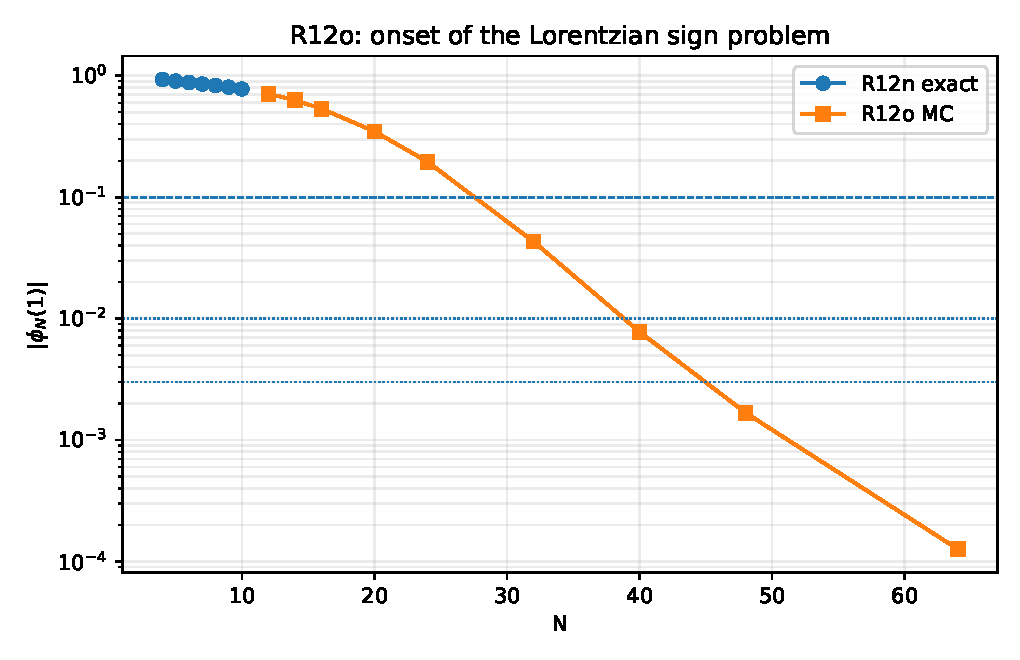
\includegraphics[width=0.75\textwidth]{r12o_phase_ratio.pdf}
\caption{R12o. L'average phase a $g=1$ diminuisce rapidamente con $N$. Il Monte Carlo diretto resta robusto nella prima parte della griglia, ma entra nel regime di sign problem severo e poi statisticamente non risolto.}
\end{figure}

Il diagnostico secondario sulla griglia congelata $g=0.25,0.5,0.75,1$ mostra esplicitamente che il problema e legato alla fase oscillante: a $N=64$ si trovano, rispettivamente,
\begin{equation}
 |\phi_{64}|\simeq0.458,\quad0.0484,\quad1.13\times10^{-3},\quad1.26\times10^{-4}.
\end{equation}
Il protocollo, tuttavia, proibisce di spostare il coupling primario verso valori piu facili dopo aver osservato questa struttura.

\begin{figure}[htbp]
\centering
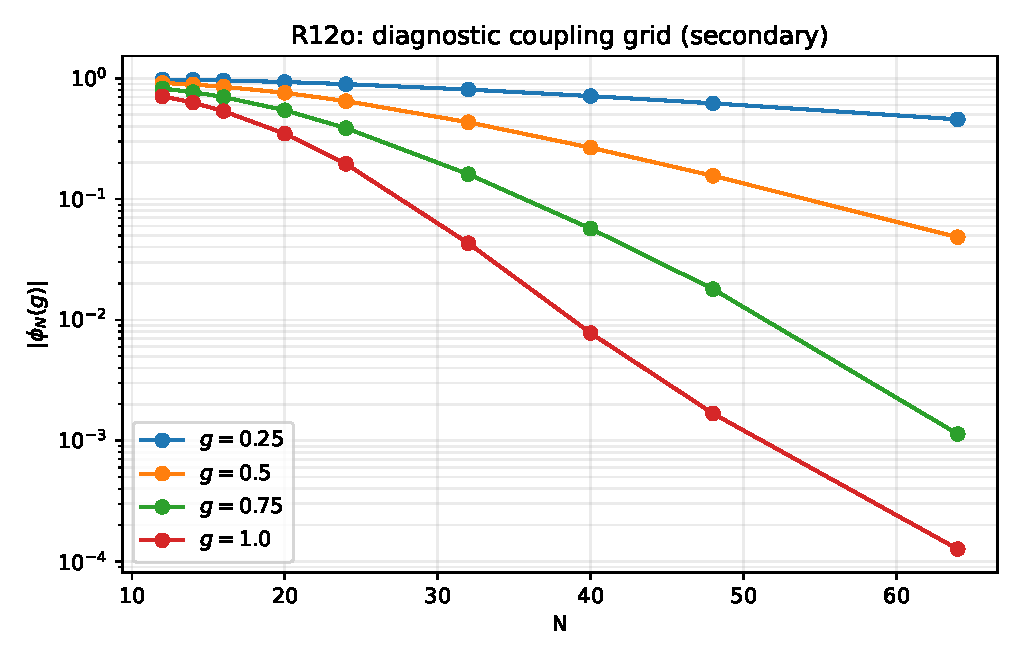
\includegraphics[width=0.75\textwidth]{r12o_phase_grid.pdf}
\caption{R12o. Griglia diagnostica secondaria del modulo della characteristic function. Ridurre $g$ ritarda l'onset delle cancellazioni, ma $g=1$ resta il coupling primario congelato.}
\end{figure}

\subsection{Lo scaling resta non classificabile}

Soltanto cinque taglie dell'estensione, $N=12$--$24$, superano il quality gate. Le pendenze effettive adiacenti in questa finestra sono
\begin{equation}
 1.801,\qquad1.928,\qquad1.805,\qquad1.610,
\end{equation}
quindi la direzione diagnostica affidabile e superestensiva e non prosegue banalmente il fit small-$N$ $\gamma_Q^{\rm rep}=1.1807$ di R12n. Tuttavia la preregistrazione richiede almeno sei taglie valide per autorizzare il fit primario. Non e quindi consentito trasformare i cinque punti disponibili in una nuova stima ufficiale di $\gamma$.

\begin{figure}[htbp]
\centering
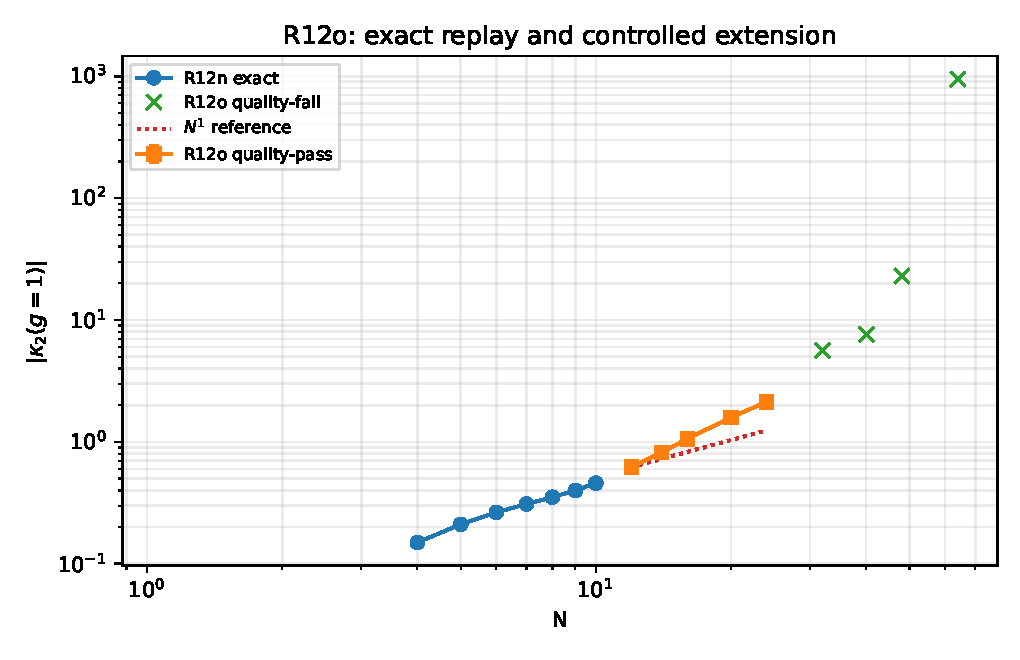
\includegraphics[width=0.75\textwidth]{r12o_lorentzian_extension.pdf}
\caption{R12o. Replay esatto R12n e estensione Monte Carlo. I quadrati pieni superano il quality gate; le croci sono stime contaminate dalle cancellazioni e non entrano in alcun fit. La linea $N^1$ e soltanto un riferimento.}
\end{figure}

Questo esito e metodologicamente informativo: il primo segnale quasi-estensivo di R12n non viene falsificato da un fit asintotico, ma la prima finestra piu grande gia mostra una deriva superestensiva prima che il sign problem impedisca di continuare con il campionamento uniforme. Il blocker non e quindi piu soltanto ``small $N$'': e ora una combinazione quantitativa di finite-size drift e cancellazioni di fase.

\subsection{Verdetto del Gate R12o}

\textbf{Gate R12o:}
\begin{quote}
\status{VALIDATED DIRECT LORENTZIAN MONTE CARLO REPRODUCES THE EXACT R12n WINDOW, BUT THE PRIMARY $g=1$ AVERAGE PHASE COLLAPSES WITH $N$ AND ONLY FIVE EXTENSION SIZES PASS THE FROZEN CUMULANT QUALITY GATE. NO PRIMARY ASYMPTOTIC $\gamma$ FIT IS AUTHORIZED. RELIABLE LOCAL SLOPES OVER $N=12$--$24$ ARE SUPEREXTENSIVE, WHILE $N\ge32$ BECOMES CUMULANT-UNRESOLVED AND $N\ge48$ PHASE-UNRESOLVED. FINAL CLASSIFICATION: FINITE\_SIZE\_OR\_SIGN\_INCONCLUSIVE.}
\end{quote}


\section{Gate R12p: ricostruzione cumulante della DOS e test di convergenza}

R12o ha mostrato che il campionamento diretto della fase a $g=1$ perde risoluzione quando $|\phi_N|$ diventa piccolo. Prima di implementare un algoritmo flat-histogram completo, R12p congela un test piu economico ma matematicamente controllabile: ricostruire la trasformata di Fourier della density of states a partire dai cumulanti ordinari della distribuzione uniforme dell'azione. Tecniche di cumulant expansion sono state usate in altri sistemi con azione complessa per trasformare il sign problem in un problema esplicito di convergenza della serie \cite{EjiriKanayaUmeda2012}; metodi density-of-states come LLR forniscono invece il benchmark successivo quando la serie non converge \cite{LangfeldLucini2014}.

Il file \texttt{PREREGISTRATION\_R12P.json} e stato scritto prima dei nuovi campioni. Restano congelati il sample space representation-weighted dei Gate R12n--R12o, $\epsilon=0.21$, il coupling $g=1$, un milione di permutazioni indipendenti per taglia e gli ordini
\begin{equation}
 K=4,6,8,10,12,
\end{equation}
con $K=10$ scelto come ricostruzione primaria prima di vedere i risultati. L'estensione $N=32$--$64$ e autorizzata soltanto se il metodo riproduce prima sia la DOS esatta $N=8,9,10$ sia il direct-MC affidabile $N=12,16,20,24$.

\subsection{Ricostruzione dalla funzione generatrice dei cumulanti}

Siano $\kappa_n$ i cumulanti ordinari dell'azione $S$ sotto la misura uniforme delle permutazioni. La characteristic function soddisfa formalmente
\begin{equation}
 \log\phi(g)=\log\langle e^{igS}\rangle
 =\sum_{n=1}^{\infty}\frac{\kappa_n(ig)^n}{n!}.
 \label{eq:r12p_logphi}
\end{equation}
La troncatura all'ordine $K$ definisce
\begin{equation}
 \phi_K(g)=\exp\left[\sum_{n=1}^{K}\frac{\kappa_n(ig)^n}{n!}\right].
\end{equation}
Poiche $-d^2\log\phi/dg^2$ e il secondo cumulante connesso nella misura complessa pesata da $e^{igS}$, la stessa serie produce
\begin{equation}
 \kappa_{2,K}^{(L)}(g)=\sum_{r=0}^{K-2}\frac{\kappa_{r+2}(ig)^r}{r!}.
 \label{eq:r12p_k2series}
\end{equation}
Questa procedura non campiona direttamente una quantita oscillante. Il prezzo e che la convergenza della serie deve essere verificata e non puo essere assunta.

\subsection{Validazione esatta e direct-MC}

\begin{table}[htbp]
\centering
\small
\begin{tabular}{rrrrr}
\toprule
$N$ & riferimento & errore $\phi_{10}$ & errore $\kappa_{2,10}$ & esito \\
\midrule
8  & exact DOS & $3.46\times10^{-4}$ & $2.20\times10^{-3}$ & PASS \\
9  & exact DOS & $5.27\times10^{-4}$ & $2.01\times10^{-3}$ & PASS \\
10 & exact DOS & $9.19\times10^{-4}$ & $2.77\times10^{-3}$ & PASS \\
12 & direct MC & $1.35\times10^{-3}$ & $7.24\times10^{-3}$ & PASS \\
16 & direct MC & $2.14\times10^{-3}$ & $1.02\times10^{-2}$ & PASS \\
20 & direct MC & $3.95\times10^{-3}$ & $1.72\times10^{-2}$ & PASS \\
24 & direct MC & $1.62\times10^{-2}$ & $6.54\times10^{-1}$ & \textbf{FAIL} \\
\bottomrule
\end{tabular}
\caption{R12p: validazione preregistrata della ricostruzione cumulante. Le soglie congelate erano $0.5\%/2\%$ per exact DOS e $3\%/10\%$ per il direct-MC rispettivamente su $\phi$ e $\kappa_2$.}
\end{table}

Il fallimento a $N=24$ non e un semplice rumore della stima diretta. Il valore direct-MC e
\begin{equation}
 |\kappa_2|_{\rm direct}=2.1746,
\end{equation}
mentre le troncature successive danno
\begin{equation}
 |\kappa_{2,8}|=1.7115,\qquad |\kappa_{2,10}|=3.3438,\qquad |\kappa_{2,12}|=1.6903.
\end{equation}
La differenza relativa $K=8\to10$ e circa $58\%$, mentre $K=10\to12$ supera il $150\%$, contro la soglia congelata del $10\%$.

\begin{figure}[htbp]
\centering
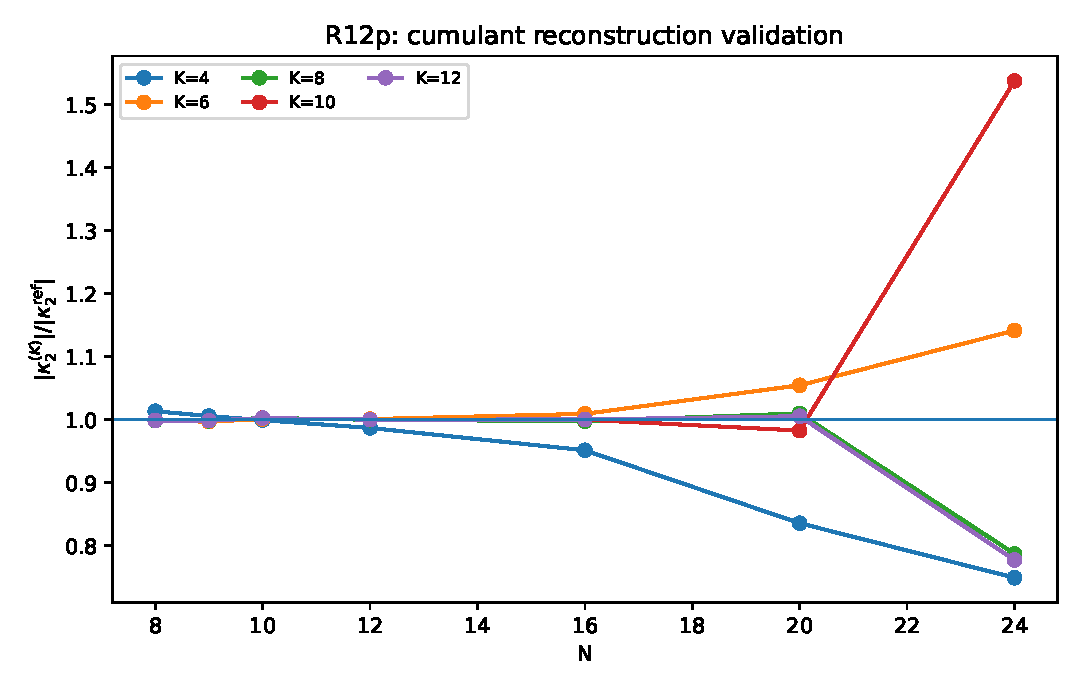
\includegraphics[width=0.78\textwidth]{r12p_cumulant_validation.pdf}
\caption{R12p. Rapporto tra il modulo del cumulante ricostruito ai diversi ordini e il riferimento exact/direct. Fino a $N=20$ le troncature convergono; a $N=24$ il settore del secondo cumulante perde stabilita.}
\end{figure}

\begin{figure}[htbp]
\centering
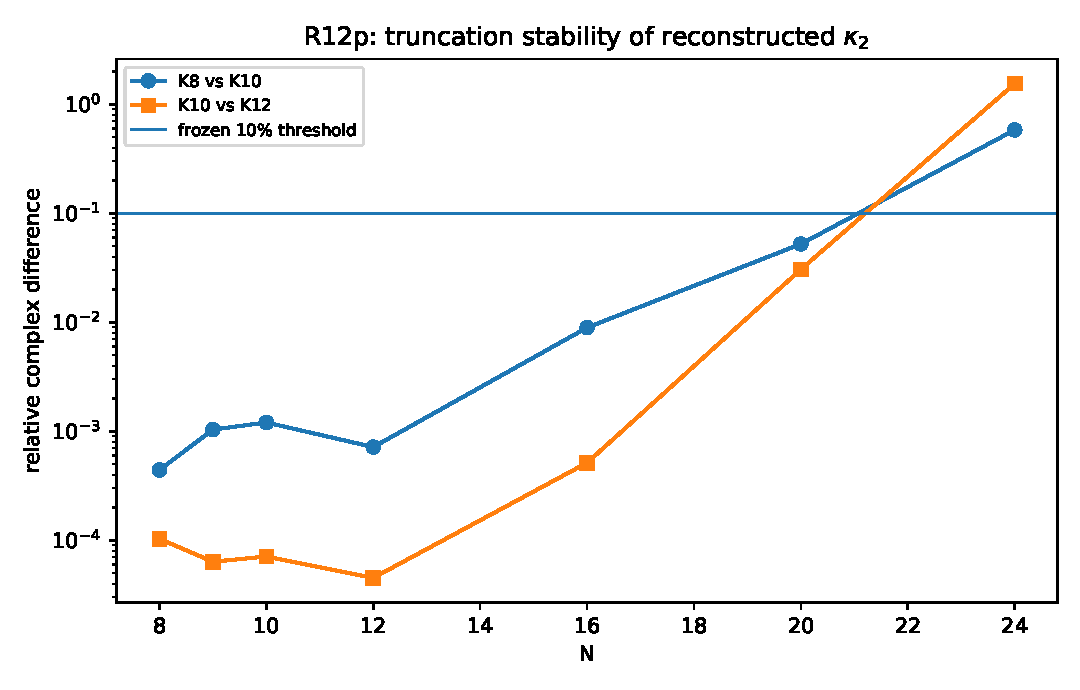
\includegraphics[width=0.75\textwidth]{r12p_truncation_stability.pdf}
\caption{R12p. Stabilita tra troncature successive della serie per $\kappa_2$. La soglia del $10\%$ era preregistrata; il suo superamento a $N=24$ blocca automaticamente l'estensione.}
\end{figure}

La characteristic function stessa resta apparentemente meglio comportata: a $N=24$ l'errore di $|\phi_{10}|$ e ancora solo dell'ordine del percento. Il problema nasce nelle derivate di $\log\phi$, che amplificano i cumulanti di ordine alto e sono proprio le quantita necessarie per il nostro test di scaling. Pertanto un buon fit della sola average phase non sarebbe sufficiente.

\subsection{Verdetto del Gate R12p}

Il protocollo vietava esplicitamente di campionare l'estensione se una sola taglia della validazione direct-MC avesse fallito. Di conseguenza non sono stati generati risultati R12p per $N=32,40,48,64$ e nessun esponente $\gamma_{\rm CE}$ viene fittato.

\textbf{Gate R12p:}
\begin{quote}
\status{THE CUMULANT/FOURIER RECONSTRUCTION PASSES THE EXACT $N=8$--$10$ WINDOW AND THE DIRECT-MC BENCHMARK THROUGH $N=20$, BUT FAILS THE FROZEN $N=24$ CONNECTED-CUMULANT VALIDATION AND TRUNCATION-STABILITY TEST. THE SIGN PROBLEM HAS BEEN CONVERTED INTO A NONCONVERGENT HIGH-ORDER-CUMULANT PROBLEM, NOT SOLVED. NO $N\ge32$ EXTENSION IS AUTHORIZED. FINAL CLASSIFICATION:} \texttt{CE\_METHOD\_VALIDATION\_FAIL}.
\end{quote}

Il risultato restringe la scelta metodologica successiva: il Gate R12q dovra usare una vera ricostruzione della density of states (LLR/flat-histogram o metodo equivalente con controllo esponenziale degli errori), non una semplice espansione locale attorno a $g=0$.

\section{Gate R12q: density of states globale con flat histogram}

R12p ha mostrato che una espansione locale di $\log\phi$ attorno a $g=0$ puo riprodurre la characteristic function ma perdere il secondo cumulante connesso quando i cumulanti di ordine alto diventano importanti. R12q cambia quindi oggetto numerico: invece di ricostruire la DOS dai momenti locali, tenta di campionare globalmente lo spazio delle azioni con un algoritmo flat-histogram. L'idea generale appartiene alla famiglia Wang--Landau/LLR, sviluppata per stimare densita di stati su molti ordini di grandezza e, nelle versioni LLR, per ottenere una soppressione esponenziale dell'errore relativo \cite{LangfeldLuciniRago2012,LangfeldLucini2014,LangfeldEtAl2016}.

Il file \texttt{PREREGISTRATION\_R12Q.json} e stato scritto e hashato prima delle nuove esecuzioni. Restano fissati il sample space representation-weighted dei Gate R12n--R12p, $\epsilon=0.21$, il coupling primario $g=1$, bin di larghezza
\begin{equation}
 \Delta S=0.05,
\end{equation}
quattro repliche Wang--Landau indipendenti per ogni $N$, la schedule $\log f:1\to10^{-5}$ per dimezzamenti, flatness minima $H_{\min}/\bar H\ge0.70$ e un successivo run multicanonico a DOS congelata. La validazione esatta usa $N=8,9,10$; quella direct-MC usa $N=12,16,20,24$. L'estensione $N=32,40,48,64$ e vietata se il metodo non supera prima sia i test numerici sia il requisito di almeno tre repliche convergenti su quattro.

\subsection{Estimatore globale e correzione multicanonica}

Sia $G_j$ la massa della density of states nel bin $j$. Wang--Landau costruisce una stima $\widehat G_j$ modificando iterativamente $\log\widehat G_j$ in modo da rendere approssimativamente piatta la visita dei bin. Dopo il congelamento di $\widehat G_j$, la produzione usa la misura
\begin{equation}
 \pi_{\rm MUCA}(C)\propto \frac{1}{\widehat G_{b(S_C)}}.
\end{equation}
Poiche il peso dipende soltanto dal bin, all'interno di ogni bin le configurazioni restano uniformi. Per ridurre l'errore di discretizzazione, la fase non viene valutata al centro del bin: per ogni configurazione visitata si conserva il valore effettivo $S_C$ e si ricostruiscono direttamente
\begin{equation}
 Z_0\propto\sum_t e^{\log\widehat G_{b_t}},\qquad
 Z_n(g)\propto\sum_t e^{\log\widehat G_{b_t}}S_t^n e^{igS_t},
\end{equation}
con $n=0,1,2$. Di conseguenza
\begin{equation}
 \phi=\frac{Z_0(g)}{Z_0(0)},\qquad
 \kappa_2=\frac{Z_2}{Z_0}-\left(\frac{Z_1}{Z_0}\right)^2.
\end{equation}
Il binning controlla dunque la stima globale della DOS, ma non sostituisce $S$ con un valore discreto nella trasformata di Fourier.

\subsection{Validazione: precisione alta quando il flat-histogram converge}

\begin{table}[htbp]
\centering
\small
\begin{tabular}{rrrrrr}
\toprule
$N$ & rif. & repliche valide & errore $\phi$ & errore $\kappa_2$ & robustezza \\
\midrule
8  & exact & $4/4$ & $0.13\%$ & $0.12\%$ & PASS \\
9  & exact & $2/4$ & $0.12\%$ & $0.40\%$ & \textbf{FAIL} \\
10 & exact & $3/4$ & $0.37\%$ & $0.28\%$ & PASS \\
12 & direct & $1/4$ & $0.59\%$ & $2.40\%$ & \textbf{FAIL} \\
16 & direct & $4/4$ & $0.91\%$ & $1.28\%$ & PASS \\
20 & direct & $4/4$ & $0.57\%$ & $3.26\%$ & PASS \\
24 & direct & $4/4$ & $1.38\%$ & $1.80\%$ & PASS \\
\bottomrule
\end{tabular}
\caption{R12q. La colonna degli errori usa la mediana componente-per-componente delle sole repliche che hanno raggiunto la stopping rule congelata. Tutte le stime numeriche disponibili soddisfano le rispettive soglie di accuratezza. Il gate fallisce pero il requisito preregistrato di almeno $3/4$ repliche valide a ogni taglia di validazione.}
\end{table}

Il punto piu importante e quindi una separazione tra \emph{accuracy} e \emph{robustness}. Quando il random walk completa la schedule, il confronto con la DOS esatta o con il direct-MC e eccellente fino a $N=24$: l'errore relativo complesso massimo sul cumulante nei casi robusti e soltanto di pochi percento. Tuttavia il criterio era volutamente piu severo: il metodo non puo dipendere dalla fortuna di una singola replica.

\begin{figure}[htbp]
\centering
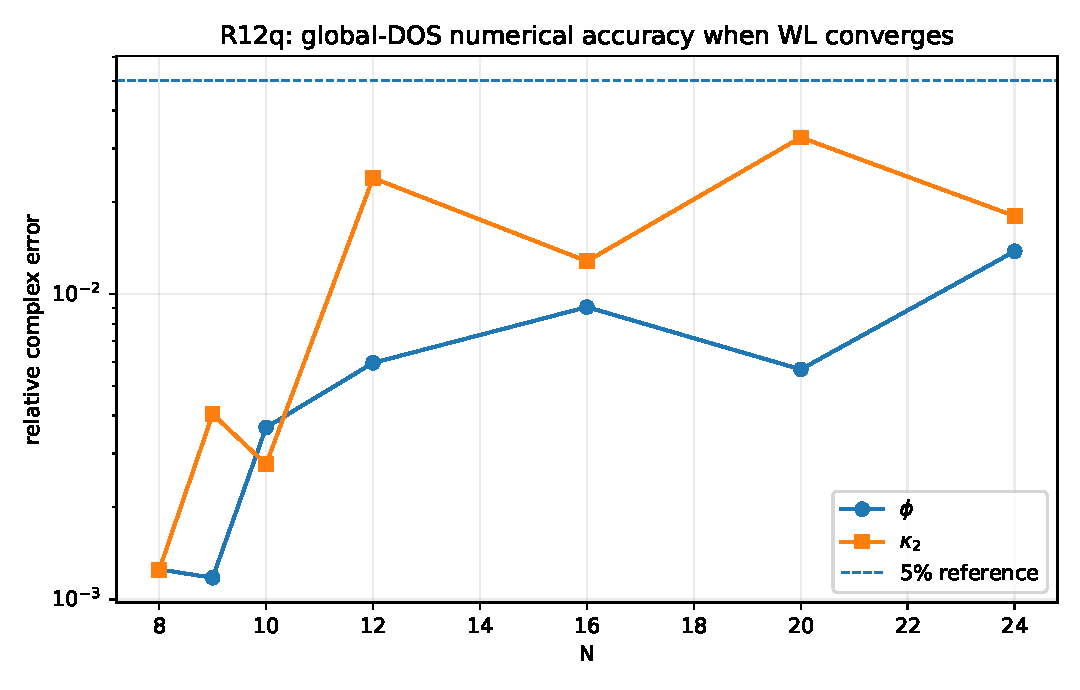
\includegraphics[width=0.76\textwidth]{r12q_dos_validation.pdf}
\caption{R12q. Errore relativo complesso della characteristic function e del secondo cumulante connesso rispetto a exact DOS/direct-MC. I valori mostrano che il core della ricostruzione globale e accurato quando il processo Wang--Landau converge.}
\end{figure}

\begin{figure}[htbp]
\centering
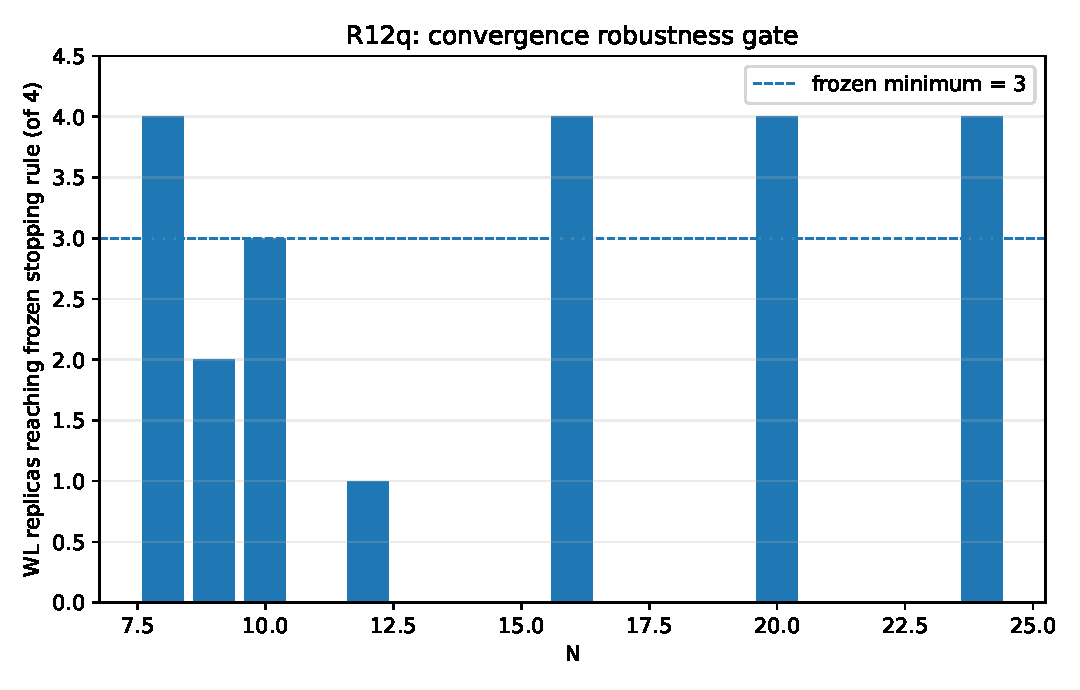
\includegraphics[width=0.76\textwidth]{r12q_wl_replica_gate.pdf}
\caption{R12q. Numero di repliche su quattro che raggiungono la stopping rule congelata. Il minimo preregistrato e tre. $N=9$ e $N=12$ bloccano quindi il gate prima di ogni estensione.}
\end{figure}

\subsection{Perche non viene modificata la schedule}

Il fallimento avrebbe potuto essere ``riparato'' aumentando selettivamente il numero massimo di proposal, rilassando la flatness o cambiando la larghezza dei bin soltanto per $N=9$ e $N=12$. Tutte queste operazioni erano esplicitamente vietate dalla preregistrazione. Il risultato va quindi interpretato come informazione sull'algoritmo scelto: il flat-histogram binned standard e capace di alta accuratezza, ma la schedule fissata non fornisce una convergenza sufficientemente robusta su tutte le taglie di controllo.

Questo suggerisce una distinzione metodologica importante. LLR non richiede di rendere globalmente piatto un istogramma: stima localmente la derivata $d\log\rho/dS$ in finestre vincolate e ricostruisce poi $\rho$ con errore relativo quasi uniforme su molti ordini di grandezza \cite{LangfeldEtAl2016}. Pertanto il fallimento di R12q non costituisce un fallimento della strategia density-of-states in generale, ma del particolare schema Wang--Landau binned e della sua stopping rule congelata.

\subsection{Verdetto del Gate R12q}

Tutti i confronti numerici disponibili passano le soglie di accuratezza, ma la qualita delle repliche fallisce a $N=9$ e $N=12$. Come preregistrato, nessun campione $N=32,40,48,64$ e stato generato e nessun $\gamma_{\rm DOS}$ viene fittato.

\textbf{Gate R12q:}
\begin{quote}
\status{GLOBAL DOS RECONSTRUCTION IS NUMERICALLY ACCURATE WHEN THE WANG--LANDAU REPLICA REACHES THE FROZEN STOPPING RULE, BUT THE PREREGISTERED REPLICA-ROBUSTNESS GATE FAILS AT $N=9$ AND $N=12$. THE FLAT-HISTOGRAM SCHEDULE IS THEREFORE NOT VALIDATED AS A ROBUST SIGN-PROBLEM MITIGATION METHOD FOR THIS BENCHMARK. NO $N>24$ EXTENSION IS AUTHORIZED. FINAL CLASSIFICATION:} \texttt{DOS\_METHOD\_VALIDATION\_FAIL}.
\end{quote}

Questa failure mode motiva direttamente R12r, riportato nella sezione successiva: una implementazione LLR histogram-free con finestre e Robbins--Monro/root finding preregistrati viene sottoposta agli stessi exact/direct benchmarks prima di qualsiasi estensione.


\section{Gate R12r: LLR histogram-free della log-density of states}

R12q ha mostrato una situazione precisa: la ricostruzione globale della DOS puo essere accurata, ma una stopping rule Wang--Landau basata sulla flatness globale non converge in modo sufficientemente robusto su tutte le taglie di controllo. R12r testa quindi la strategia LLR (logarithmic linear relaxation), nella quale non si cerca un istogramma globalmente piatto. Si stima invece localmente la derivata
\begin{equation}
 a(S)=\frac{d\log\rho(S)}{dS}
\end{equation}
in una sequenza di finestre sovrapposte e si integra successivamente $a(S)$ per ricostruire $\log\rho$ a meno di una costante additiva. Questa e la caratteristica che rende LLR adatto a densita di stati con dinamica su molti ordini di grandezza e a trasformate oscillanti con forte sign problem \cite{LangfeldLuciniRago2012,LangfeldLucini2014,LangfeldEtAl2016}.

Prima del freeze sono stati usati esclusivamente $N=6,7$ come \emph{development pilot}, esplicitamente esclusi da qualunque classificazione. Il protocollo definitivo, salvato in \texttt{PREREGISTRATION\_R12R.json} e hashato prima di $N=8,9,10$, fissa $\epsilon=0.21$, $g=1$, finestre di larghezza
\begin{equation}
 \Delta S=0.6
\end{equation}
con distanza tra i centri non superiore a $0.3$, tre repliche per taglia, sei iterazioni root a guadagno pieno seguite da 24 iterazioni Robbins--Monro, e $2000+6000$ proposal per iterazione tra burn-in e misura. In ciascuna finestra il parametro $a$ viene aggiornato secondo
\begin{equation}
 a_{n+1}=a_n+g_n\frac{12}{(\Delta S)^2}\left\langle S-S_c\right\rangle_{a_n},
\end{equation}
con $g_n=1$ nella fase iniziale e $g_n=1/n$ nella fase Robbins--Monro. Il root locale e definito dalla condizione
\begin{equation}
 \left\langle S-S_c\right\rangle_a=0.
\end{equation}
Una volta ottenute le pendenze, esse vengono interpolate e integrate numericamente; la trasformata oscillante usa poi
\begin{equation}
 Z_m(g)=\int dS\,\rho(S)S^m e^{igS},\qquad
 \kappa_2=\frac{Z_2}{Z_0}-\left(\frac{Z_1}{Z_0}\right)^2.
\end{equation}

\subsection{Amendment tecnici fail-closed}

Durante la prima esecuzione $N=9$ ha rivelato due problemi puramente esecutivi. Il primo era che il codice conservava soltanto il seed di overlap dell'ultima iterazione Robbins--Monro: se quella singola iterazione non visitava una meta della finestra, il seed precedente veniva perso. \texttt{AMENDMENT\_01\_R12R\_OVERLAP\_SEED.json} rende persistente l'ultimo vero stato campionato nell'overlap, senza modificare proposal, root schedule, finestre, seed casuali o soglie. Una esecuzione diagnostica successiva ha mostrato che una replica continuava comunque a fermarsi perche la finestra precedente aveva gia fallito il quality gate e quindi non possedeva alcun seed valido. \texttt{AMENDMENT\_02\_R12R\_FAILCLOSED\_REPLICA.json} implementa semplicemente la logica gia preregistrata: appena una finestra fallisce, l'intera replica e marcata invalida e non viene usata nell'aggregazione. Nessuno dei due amendment cambia la statistica ammessa dal gate.

\subsection{Exact validation e fallimento di robustezza}

La preregistrazione richiede almeno due repliche valide su tre per ogni $N$. Inoltre, per le taglie exact, la mediana componente-per-componente delle repliche valide deve rispettare errore relativo complesso $<3\%$ su $\phi$ e $<12\%$ su $\kappa_2$. Il risultato e:

\begin{table}[htbp]
\centering
\small
\begin{tabular}{rrrrr}
\toprule
$N$ & repliche valide & errore $\phi$ & errore $\kappa_2$ & gate \\
\midrule
8  & $2/3$ & $2.90\%$ & $10.79\%$ & PASS \\
9  & $1/3$ & -- & -- & \textbf{FAIL} \\
10 & $1/3$ & -- & -- & \textbf{FAIL} \\
\bottomrule
\end{tabular}
\caption{R12r. La accuratezza aggregata viene classificata solo quando esistono almeno due repliche valide, come fissato prima dei risultati. $N=8$ passa entrambe le soglie; $N=9$ e $N=10$ falliscono gia il requisito di robustezza.}
\end{table}

Le singole repliche che riescono a soddisfare tutti i window gate non mostrano un collasso numerico della ricostruzione. A titolo diagnostico, l'unica replica valida di $N=9$ ha errore complesso circa $0.14\%$ su $\phi$ e $7.0\%$ su $\kappa_2$; per $N=10$ gli errori sono circa $1.29\%$ e $3.46\%$. Questi valori non possono pero essere usati per salvare il gate: la condizione preregistrata riguarda la ripetibilita tra repliche, non l'esistenza di una singola traiettoria fortunata.

\begin{figure}[htbp]
\centering
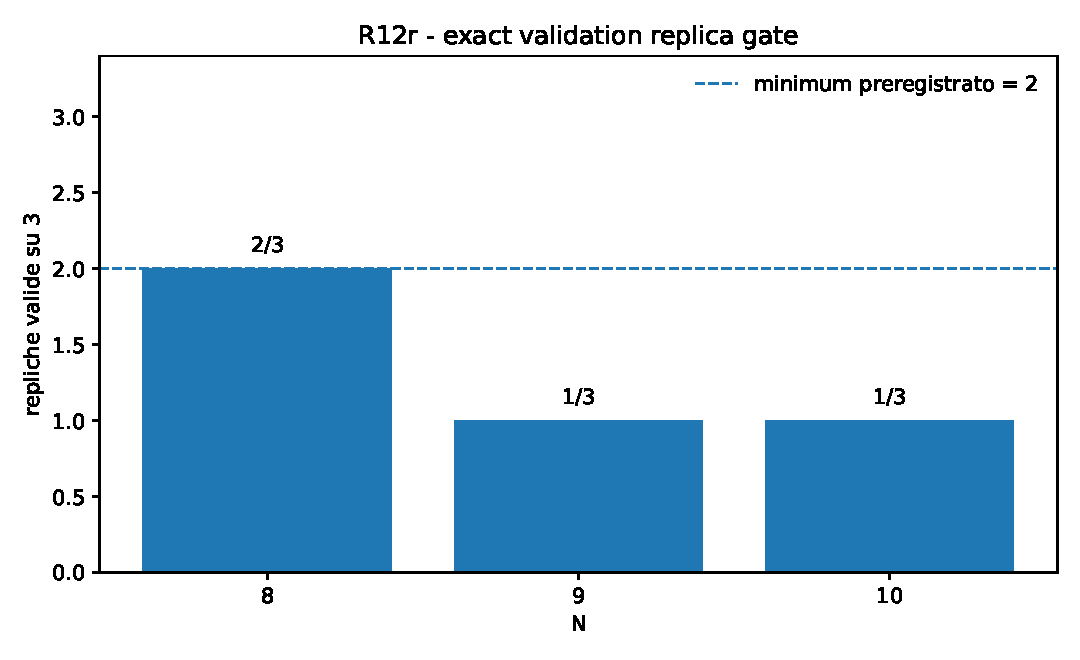
\includegraphics[width=0.70\textwidth]{r12r_llr_replica_gate.pdf}
\caption{R12r. Numero di repliche LLR che superano tutte le finestre locali. Il minimo congelato e due su tre. Le taglie $N=9$ e $N=10$ bloccano il metodo prima della direct validation.}
\end{figure}

\subsection{Verdetto del Gate R12r}

Il fallimento avviene gia nell'exact stage. Pertanto il protocollo vieta di eseguire la direct validation $N=12,16,20,24$ e, a maggior ragione, l'estensione $N=32,40,48,64$. Nessun esponente $\gamma_{\rm LLR}$ viene fittato.

\textbf{Gate R12r:}
\begin{quote}
\status{THE HISTOGRAM-FREE LLR CORE CAN REPRODUCE THE EXACT LORENTZIAN DOS WHEN A REPLICA SOLVES ALL LOCAL WINDOWS, BUT THE FROZEN REPLICA-ROBUSTNESS GATE FAILS ALREADY AT $N=9$ AND $N=10$: ONLY ONE OF THREE REPLICAS IS VALID AT EACH SIZE, BELOW THE PREREGISTERED MINIMUM OF TWO. DIRECT VALIDATION AND ALL $N>24$ EXTENSIONS ARE THEREFORE FORBIDDEN. FINAL CLASSIFICATION:} \texttt{LLR\_METHOD\_VALIDATION\_FAIL}.
\end{quote}

R12q e R12r mostrano quindi due failure mode complementari: la DOS globale binned e accurata ma puo non completare una schedule di flatness; la LLR locale evita la flatness globale ma puo perdere robustezza nelle finestre di coda con hard boundaries. Il successivo R12s dovra percio testare una stratificazione con \emph{soft windows} e scambio tra finestre/umbrella reweighting (WHAM/MBAR o equivalente), mantenendo gli stessi exact/direct benchmarks e senza modificare $g$, sample space o criteri dopo i risultati.


\section{Gate R12s: soft-window umbrella, replica exchange e MBAR}

R12q e R12r hanno fallito per ragioni complementari legate alle \emph{hard boundaries}: il Wang--Landau globale puo non completare la stopping rule di flatness, mentre LLR puo perdere una replica quando una finestra di coda non soddisfa il quality gate. R12s rimuove quindi la discontinuita del vincolo e usa umbrella armoniche sovrapposte,
\begin{equation}
 U_i(S)=\frac{\kappa}{2}(S-c_i)^2,
\end{equation}
con scambi Metropolis tra finestre adiacenti. L'idea di umbrella sampling risale alla costruzione di Torrie e Valleau \cite{TorrieValleau1977}; la ricombinazione delle distribuzioni biased viene qui effettuata con le equazioni MBAR, che evitano la discretizzazione in istogrammi della variabile di reweighting \cite{ShirtsChodera2008}. Per ogni campione con azione $S_n$ si costruisce
\begin{equation}
 u_i(S_n)=\frac{\kappa}{2}(S_n-c_i)^2,
\end{equation}
mentre gli offset di free energy $f_i$ soddisfano le equazioni autoconsistenti
\begin{equation}
 e^{-f_i}
 =\sum_n
 \frac{e^{-u_i(S_n)}}{\sum_j N_j e^{f_j-u_j(S_n)}}.
\end{equation}
Una volta risolto il sistema, il peso unbiased di ciascun campione e proporzionale a
\begin{equation}
 w_n\propto
 \left[\sum_j N_j e^{f_j-u_j(S_n)}\right]^{-1},
\end{equation}
e le quantita Lorentziane vengono valutate direttamente ai valori reali campionati,
\begin{equation}
 \phi(g)=\sum_n w_n e^{igS_n},\qquad
 \kappa_2(g)=\frac{\sum_n w_n S_n^2 e^{igS_n}}{\phi(g)}
 -\left(\frac{\sum_n w_n S_n e^{igS_n}}{\phi(g)}\right)^2.
\end{equation}
Non viene quindi introdotto alcun binning artificiale nella fase $e^{igS}$.

\subsection{Preregistrazione e development pilot escluso}

Prima del freeze sono stati usati soltanto $N=6,7$ come development pilot, esclusi da ogni classificazione. Il protocollo definitivo e registrato in \texttt{PREREGISTRATION\_R12S.json}, SHA--256
\begin{center}
\texttt{69c580955a5ec1dc0817baeb221045729c568b9960d64c2571f0b3c945a42764}.
\end{center}
Sono fissati prima dell'exact validation: $\epsilon=0.21$, $g=1$, spacing dei centri $0.8$, $\kappa=1$, tre repliche indipendenti per taglia, $10^4$ cicli di burn-in, $4\times10^4$ cicli di produzione, thinning ogni 20 cicli e tentativi di exchange ogni due cicli. Il supporto di ciascuna replica viene congelato da un pilot uniforme di $5\times10^4$ permutazioni, allargato di $0.8$ deviazioni standard su ciascun lato. Una replica deve soddisfare simultaneamente acceptance locale ed exchange $\geq0.15$, ESS per finestra $\geq400$, ESS dei pesi unbiased $\geq1000$, convergenza MBAR $<10^{-8}$ e diffusione delle label su almeno meta delle finestre. Per ogni $N$ occorrono almeno due repliche coerenti su tre.

Il development pilot aveva errori exact inferiori a circa $0.5\%$ su $\phi$ e $1.6\%$ su $\kappa_2$, con exchange minima $\simeq0.72$--$0.75$ e ESS per finestra $\simeq1800$--$1900$. Nessun parametro e stato cambiato dopo l'hash della preregistrazione.

\subsection{Exact validation: pieno PASS}

La prima barriera e R12n exact su $N=8,9,10$. Tutte le nove repliche individuali superano i quality gate e tutte le repliche restano coerenti con la mediana componente-per-componente. Gli errori complessi aggregati sono:
\begin{table}[htbp]
\centering
\small
\begin{tabular}{rrrrr}
\toprule
$N$ & repliche valide & errore $\phi$ & errore $\kappa_2$ & gate \\
\midrule
8  & $3/3$ & $0.44\%$ & $0.75\%$ & PASS \\
9  & $3/3$ & $0.30\%$ & $0.44\%$ & PASS \\
10 & $3/3$ & $0.42\%$ & $0.87\%$ & PASS \\
\bottomrule
\end{tabular}
\caption{R12s exact validation. Le soglie congelate sono $3\%$ per $\phi$ e $10\%$ per $\kappa_2$.}
\end{table}
Questa e la prima strategia di reconstruction successiva a R12o che attraversa l'intero exact gate senza perdita di repliche.

\subsection{Direct validation: PASS fino a $N=20$, fail-closed a $N=24$}

Superato l'exact gate, il protocollo autorizza il confronto con i benchmark uniformi congelati di R12o. I risultati sono:
\begin{table}[htbp]
\centering
\small
\begin{tabular}{rrrrr}
\toprule
$N$ & repliche usate & errore $\phi$ & errore $\kappa_2$ & gate \\
\midrule
12 & $3/3$ & $0.16\%$ & $1.34\%$ & PASS \\
16 & $3/3$ & $1.03\%$ & $3.43\%$ & PASS \\
20 & $3/3$ & $1.57\%$ & $5.79\%$ & PASS \\
24 & $2/3$ & $5.84\%$ & $15.33\%$ & \textbf{FAIL} \\
\bottomrule
\end{tabular}
\caption{R12s direct validation. Le soglie congelate sono $5\%$ per $\phi$ e $15\%$ per $\kappa_2$. A $N=24$ una replica viene inoltre esclusa dal consistency gate, lasciandone comunque le due minime richieste.}
\end{table}

\begin{figure}[htbp]
\centering
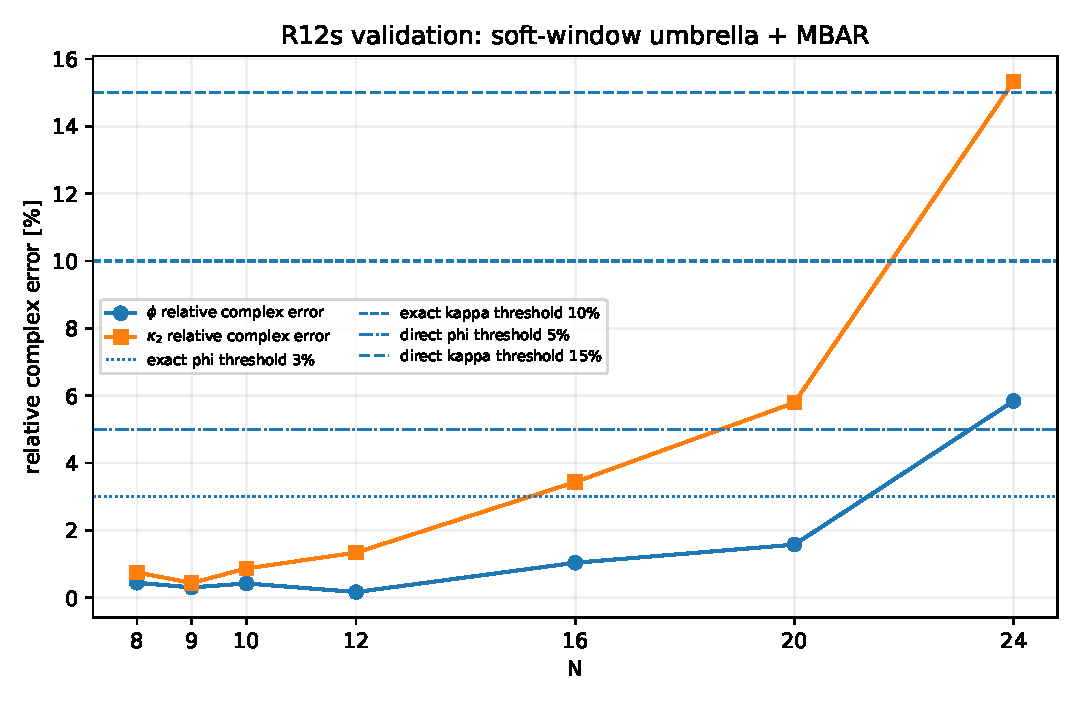
\includegraphics[width=0.76\textwidth]{r12s_validation_errors.pdf}
\caption{R12s. Errori complessi rispetto a R12n exact e R12o direct. Il metodo resta accurato fino a $N=20$; a $N=24$ oltrepassa di poco entrambe le soglie direct congelate.}
\end{figure}

\begin{figure}[htbp]
\centering
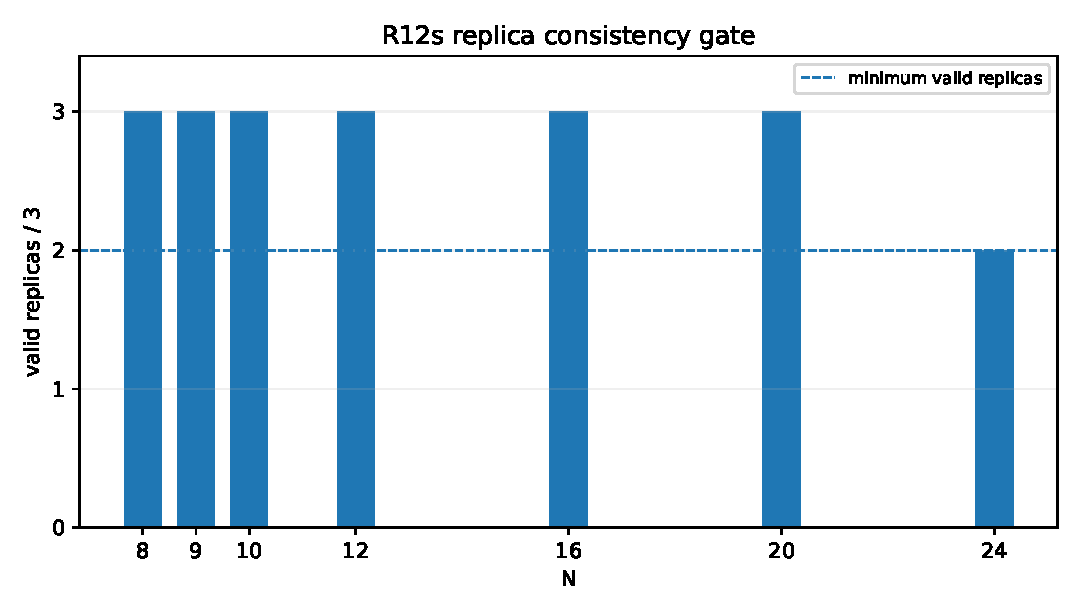
\includegraphics[width=0.68\textwidth]{r12s_replica_gate.pdf}
\caption{R12s. Replica consistency gate. Exact e direct fino a $N=20$ mantengono tre repliche valide; a $N=24$ ne restano due, ancora sufficienti, ma l'accuratezza aggregata fallisce le soglie preregistrate.}
\end{figure}

Il failure a $N=24$ e quantitativamente marginale ma metodologicamente netto: $5.84\%>5\%$ e $15.33\%>15\%$. Aumentare la statistica soltanto su questa taglia, allargare la tolleranza o includere la replica incoerente dopo aver visto il risultato avrebbe violato la preregistrazione. Pertanto nessun $N=32,40,48,64$ viene eseguito e non viene fittato alcun $\gamma_{\rm R12s}$.

\subsection{Verdetto del Gate R12s}

\textbf{Gate R12s:}
\begin{quote}
\status{SOFT HARMONIC UMBRELLAS, REPLICA EXCHANGE AND MBAR REMOVE THE HARD-WINDOW ROBUSTNESS FAILURE: EXACT $N=8$--$10$ PASSES WITH THREE OF THREE VALID REPLICAS AND SUB-PERCENT ERRORS, AND DIRECT $N=12$--$20$ PASSES COMFORTABLY. HOWEVER THE FROZEN DIRECT GATE FAILS AT $N=24$: AFTER THE CONSISTENCY FILTER TWO REPLICAS REMAIN, BUT THE COMPLEX ERRORS ARE $5.84\%$ FOR $\phi$ AND $15.33\%$ FOR $\kappa_2$, SLIGHTLY ABOVE THE PREREGISTERED $5\%$ AND $15\%$ LIMITS. NO $N>24$ EXTENSION IS AUTHORIZED. FINAL CLASSIFICATION:} \texttt{R12S\_METHOD\_VALIDATION\_FAIL}.
\end{quote}

R12s localizza ulteriormente il blocker. La mobilita tra finestre non e piu il problema dominante: exchange ed ESS restano ampiamente sopra le soglie. Il limite compare nel reweighting globale proprio quando l'average phase e gia ridotta. Il successivo R12t dovra quindi testare una stima \emph{phase-targeted} con allocazione uniforme preregistrata (non selettiva su $N=24$), per esempio bridge/stratified reweighting o un estimatore di rapporto complesso tra stati adiacenti, validato ancora una volta contro R12n e R12o prima di qualunque estensione.


\section{Gate R12t: stratificazione indipendente dei momenti complessi}

R12t evita sia una ricostruzione globale della DOS sia un singolo average phase campionato crudamente. Prima dei risultati di validazione e stato congelato il file \texttt{PREREGISTRATION\_R12T.json} (SHA-256 \texttt{3408d54f4556712ecc235fb0a41045c1f98e3e9777daf3d0f877a52660a5588f}). Il development pilot usa soltanto $N=6,7$ ed e escluso da ogni classificazione. Il sample space, l'azione, $\epsilon=0.21$ e il coupling primario $g=1$ restano identici ai Gate R12n--R12s.

Sia $\{A_j\}_{j=1}^{K}$ una partizione dell'asse dell'azione, $p_j=P(S\in A_j)$ e
\begin{equation}
 m_j^{(r)}(g)=\mathbb E\!\left[S^r e^{igS}\mid S\in A_j\right].
\end{equation}
Per la legge dell'aspettazione totale,
\begin{equation}
 M_r(g)=\sum_{j=1}^{K}p_jm_j^{(r)}(g),\qquad
 \phi(g)=M_0(g),
\end{equation}
con
\begin{equation}
 \kappa_2(g)=\frac{M_2(g)}{M_0(g)}-
 \left(\frac{M_1(g)}{M_0(g)}\right)^2.
 \label{eq:r12tstratified}
\end{equation}
La stima e costruita con tre stream indipendenti di permutazioni uniformi: $100\,000$ configurazioni definiscono 16 strati quantili empirici; $400\,000$ configurazioni indipendenti stimano le masse $p_j$; un terzo stream accumula esattamente $15\,000$ configurazioni condizionate in ogni strato. La fase $e^{igS}$ e sempre valutata sul valore reale dell'azione, senza binning. Vengono eseguite tre repliche indipendenti per ogni $N$. La stratificazione e una tecnica classica di riduzione della varianza: per una partizione fissata, separare i contributi e controllare l'allocazione per strato puo ridurre la varianza rispetto al Monte Carlo grezzo, pur lasciando invariato il valore atteso \cite{Sayah2019}.

\subsection{Replay exact e direct}

Il gate exact richiede errori complessi inferiori al $3\%$ su $\phi$ e al $10\%$ su $\kappa_2$. Tutte le repliche risultano valide e coerenti:
\begin{center}
\begin{tabular}{rccr}
\toprule
$N$ & errore $\phi$ & errore $\kappa_2$ & repliche valide \\
\midrule
8  & $0.059\%$ & $0.074\%$ & $3/3$ \\
9  & $0.100\%$ & $0.117\%$ & $3/3$ \\
10 & $0.093\%$ & $0.450\%$ & $3/3$ \\
\bottomrule
\end{tabular}
\end{center}

La direct validation contro il riferimento congelato R12o richiede $5\%$ su $\phi$ e $15\%$ su $\kappa_2$:
\begin{center}
\begin{tabular}{rccr}
\toprule
$N$ & errore $\phi$ & errore $\kappa_2$ & repliche valide \\
\midrule
12 & $0.199\%$ & $0.514\%$ & $3/3$ \\
16 & $0.221\%$ & $1.444\%$ & $3/3$ \\
20 & $0.502\%$ & $0.433\%$ & $3/3$ \\
24 & $0.843\%$ & $6.532\%$ & $3/3$ \\
\bottomrule
\end{tabular}
\end{center}

\begin{figure}[htbp]
\centering
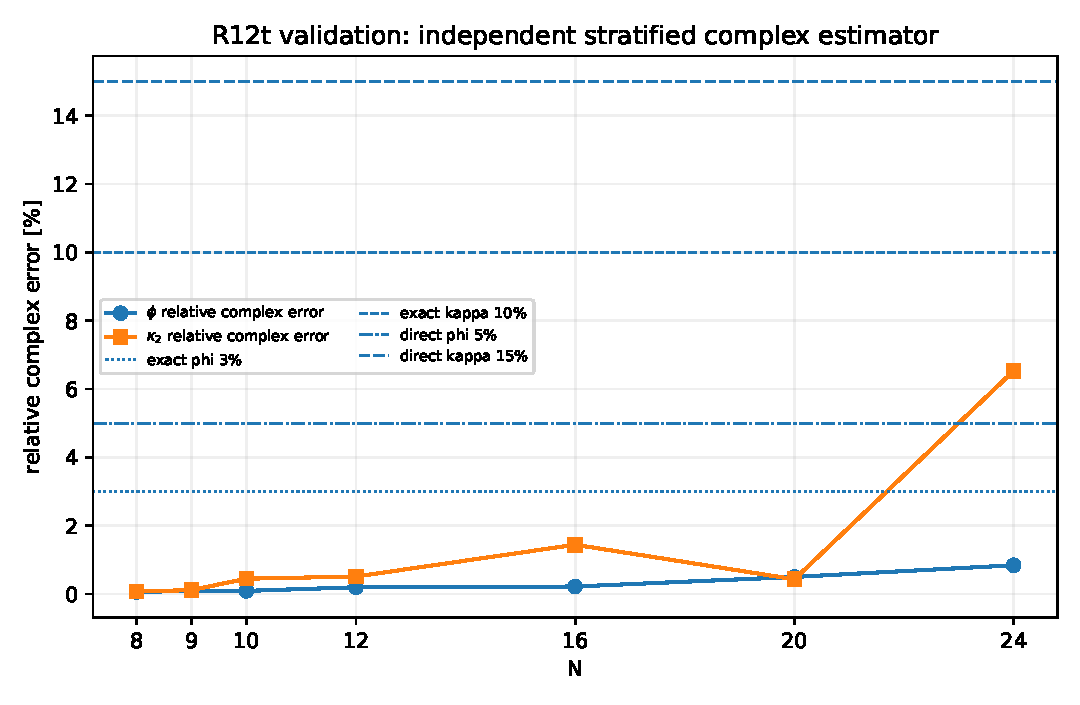
\includegraphics[width=0.77\textwidth]{r12t_validation_errors.pdf}
\caption{R12t. Replay exact/direct del nuovo estimatore stratificato. Tutte le taglie di validazione restano ampiamente dentro le soglie congelate, incluso $N=24$ che aveva bloccato R12s.}
\end{figure}

Questo e il primo metodo successivo a R12o che supera formalmente l'intero replay fino a $N=24$ e viene quindi autorizzato ad eseguire l'estensione preregistrata.

\subsection{Estensione e ritorno del sign problem}

L'estensione produce:
\begin{center}
\begin{tabular}{rccc}
\toprule
$N$ & intervallo replica $|\phi(1)|$ & intervallo replica $|\kappa_2(1)|$ & repliche coerenti \\
\midrule
32 & $0.0433$--$0.0451$ & $3.55$--$5.05$ & $2/3$ \\
40 & $0.00633$--$0.00675$ & $18.83$--$22.08$ & $1/3$ \\
48 & $0.00156$--$0.00349$ & $39.61$--$132.84$ & $0/3$ \\
64 & $0.00134$--$0.00348$ & $27.31$--$52.96$ & $0/3$ \\
\bottomrule
\end{tabular}
\end{center}

A $N=32$ il consistency gate conserva due repliche e fornisce l'aggregato
\begin{equation}
 |\phi_{32}(1)|=0.04417,\qquad |\kappa_{2,32}(1)|=4.700.
\end{equation}
Da $N=40$ in poi, invece, la dispersione complessa tra repliche supera i limiti preregistrati. La caratteristica comune e il collasso di $|\phi|$: quando il rapporto di fase scende sotto l'ordine di $10^{-2}$, una stratificazione indipendente a statistica fissata non risolve piu con robustezza le cancellazioni residue.

\begin{figure}[htbp]
\centering
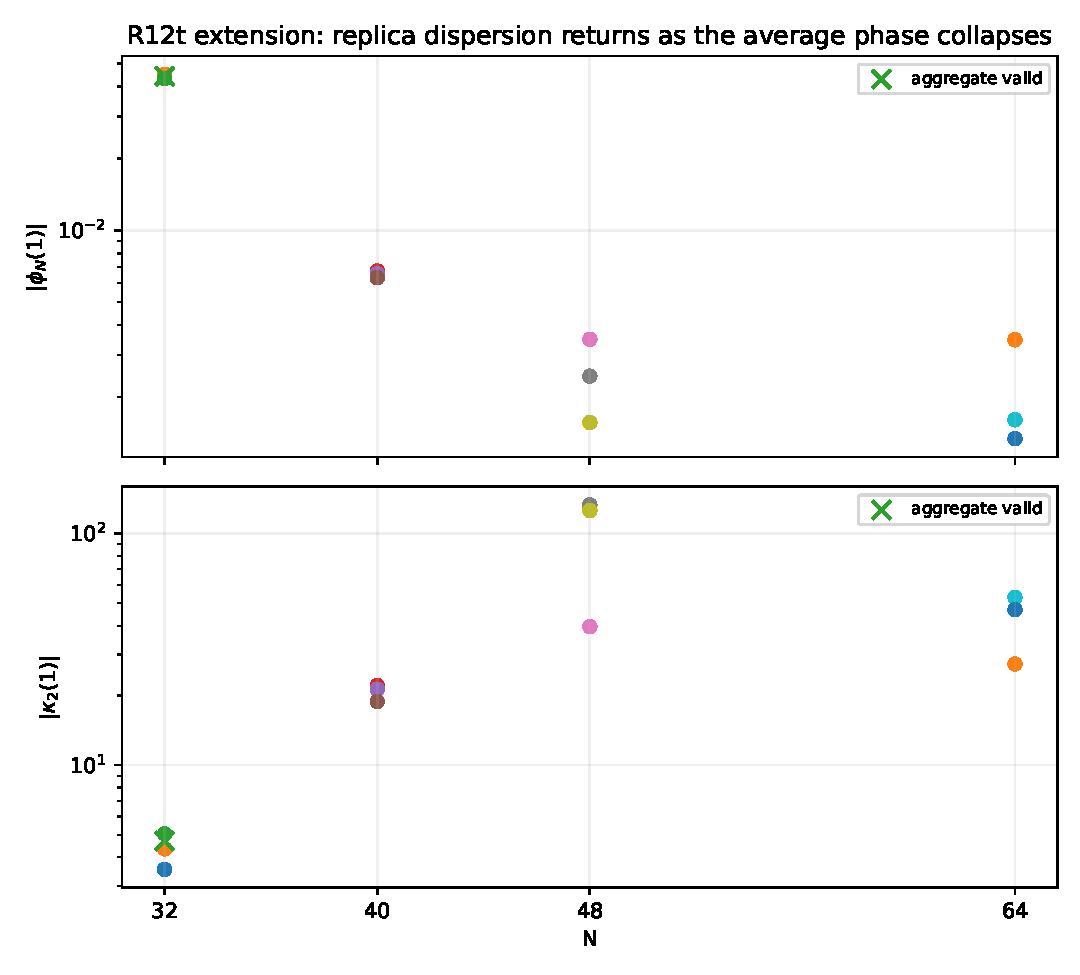
\includegraphics[width=0.76\textwidth]{r12t_extension_dispersion.pdf}
\caption{R12t extension. La stratificazione indipendente supera il precedente muro a $N=24$ e mantiene due repliche coerenti a $N=32$, ma la dispersione di $\kappa_2$ cresce rapidamente quando l'average phase scende sotto $\mathcal O(10^{-2})$.}
\end{figure}

Il fit primario richiede almeno cinque taglie fra $N=20,24,32,40,48,64$, con almeno tre taglie di estensione e almeno due repliche valide per ogni punto. Sopravvivono soltanto
\begin{equation}
 \boxed{N=20,24,32}.
\end{equation}
Pertanto il fit di $\gamma_{\rm R12t}$ e vietato. Come diagnostica secondaria, le sole pendenze locali autorizzate sono
\begin{equation}
 \gamma_{20\to24}=1.886,\qquad
 \gamma_{24\to32}=2.572,
\end{equation}
ma non costituiscono una classificazione asintotica.

\subsection{Verdetto del Gate R12t}

\textbf{Gate R12t:}
\begin{quote}
\status{INDEPENDENT ACTION STRATIFICATION WITH SEPARATE MASS AND CONDITIONAL STREAMS PASSES THE FULL EXACT $N=8$--$10$ AND DIRECT $N=12$--$24$ VALIDATION, AND THEREFORE EARNS A PREREGISTERED EXTENSION BEYOND THE PREVIOUS SIGN BARRIER. $N=32$ RETAINS TWO OF THREE CONSISTENT REPLICAS, BUT $N=40$ RETAINS ONLY ONE AND $N=48,64$ RETAIN NONE. ONLY $N=20,24,32$ SATISFY THE FROZEN SCALING-POINT REQUIREMENTS, BELOW THE REQUIRED FIVE POINTS AND THREE EXTENSION SIZES; NO GLOBAL EXPONENT IS FITTED. FINAL CLASSIFICATION:} \texttt{R12T\_FINITE\_SIZE\_OR\_PRECISION\_INCONCLUSIVE}.
\end{quote}

R12t stabilisce quindi due fatti. Primo, il fallimento R12s non era un limite fondamentale della DOS: una stima stratificata indipendente puo attraversare $N=24$ con ampio margine. Secondo, il sign problem non scompare: quando $|\phi|$ diventa dell'ordine di $10^{-2}$ o inferiore, la dispersione tra repliche torna dominante. Il successivo R12u dovra quindi ridurre direttamente la varianza della cancellazione complessa, per esempio mediante strati allineati alla fase e/o Rao--Blackwell/control variates su orbite locali, mantenendo invariati sample space, azione, $g=1$ e benchmark.


\section{Gate R12u: control variates di Lehmer e ANOVA locale}

R12u attacca direttamente la varianza dei momenti complessi senza ricostruire la DOS. Prima dei risultati di validazione e stato congelato il file \texttt{PREREGISTRATION\_R12U.json} (SHA-256 \texttt{2f5c4a0792fa25d387fa5e226b6cd2853347c05f51fe39b093ddecd31c2c6a96}). I soli development pilot, $N=6,7$, sono esclusi da ogni classificazione. Nel pilot la base scelta riduceva la trace variance dei tre target complessi a circa il $12$--$24\%$ del Monte Carlo grezzo; nessuna taglia $N\ge8$ e stata usata per scegliere la schedule finale.

Per una permutazione $p\in S_N$ definiamo il codice di Lehmer
\begin{equation}
 d_i(p)=\#\{j>i:p_j<p_i\},\qquad d_i\in\{0,\ldots,N-i-1\}.
\end{equation}
Il codice e una biiezione
\begin{equation}
 S_N\longleftrightarrow [N]\times[N-1]\times\cdots\times[1],
\end{equation}
per cui, sotto la misura uniforme sulle permutazioni, i digit $d_i$ sono mutuamente indipendenti e ciascuno e uniforme sul proprio dominio \cite{Lehmer1960}. Questa struttura fornisce control variates con media esattamente nota, senza stimare la loro normalizzazione dal campione di valutazione.

Per i tre target
\begin{equation}
 Y_r=S^r e^{iS},\qquad r=0,1,2,
\end{equation}
uno stream di training indipendente costruisce main effects $c_{r,i}(d_i)$ centrati in modo che
\begin{equation}
 \frac{1}{N-i}\sum_{v=0}^{N-i-1}c_{r,i}(v)=0,
\end{equation}
e interazioni adiacenti $c_{r,i,i+1}(d_i,d_{i+1})$ sottoposte a double-centering, cosi che la loro media sulla legge prodotto uniforme sia anch'essa esattamente nulla. Sullo stream di valutazione indipendente si usa quindi
\begin{equation}
 \widehat Z_r=\frac1M\sum_{m=1}^{M}\left[Y_r^{(m)}-\sum_i c_{r,i}(d_i^{(m)})-\sum_i c_{r,i,i+1}(d_i^{(m)},d_{i+1}^{(m)})\right].
 \label{eq:r12uCV}
\end{equation}
Condizionatamente alle tabelle di training congelate, l'aspettazione dei termini sottratti e zero esatto. Ne segue
\begin{equation}
 \mathbb E[\widehat Z_r\mid\mathrm{training}]=\mathbb E[Y_r],
\end{equation}
quindi il controllo della varianza non introduce bias da fit. Il protocollo usa $400\,000$ permutazioni di training e $800\,000$ di valutazione per replica, con 100 batch indipendenti ai fini del quality gate e tre repliche per ogni $N$.

\subsection{Replay exact e direct}

L'exact replay R12n passa integralmente:
\begin{center}
\begin{tabular}{rccc}
\toprule
$N$ & errore $\phi$ & errore $\kappa_2$ & repliche valide \\
\midrule
8  & $0.0052\%$ & $0.0477\%$ & $3/3$ \\
9  & $0.0258\%$ & $0.1201\%$ & $3/3$ \\
10 & $0.0353\%$ & $0.1694\%$ & $3/3$ \\
\bottomrule
\end{tabular}
\end{center}

Anche la direct validation contro R12o resta entro le soglie congelate:
\begin{center}
\begin{tabular}{rccc}
\toprule
$N$ & errore $\phi$ & errore $\kappa_2$ & repliche valide \\
\midrule
12 & $0.163\%$ & $0.022\%$ & $3/3$ \\
16 & $0.093\%$ & $0.679\%$ & $3/3$ \\
20 & $0.390\%$ & $0.966\%$ & $3/3$ \\
24 & $0.752\%$ & $6.242\%$ & $3/3$ \\
\bottomrule
\end{tabular}
\end{center}

\begin{figure}[htbp]
\centering
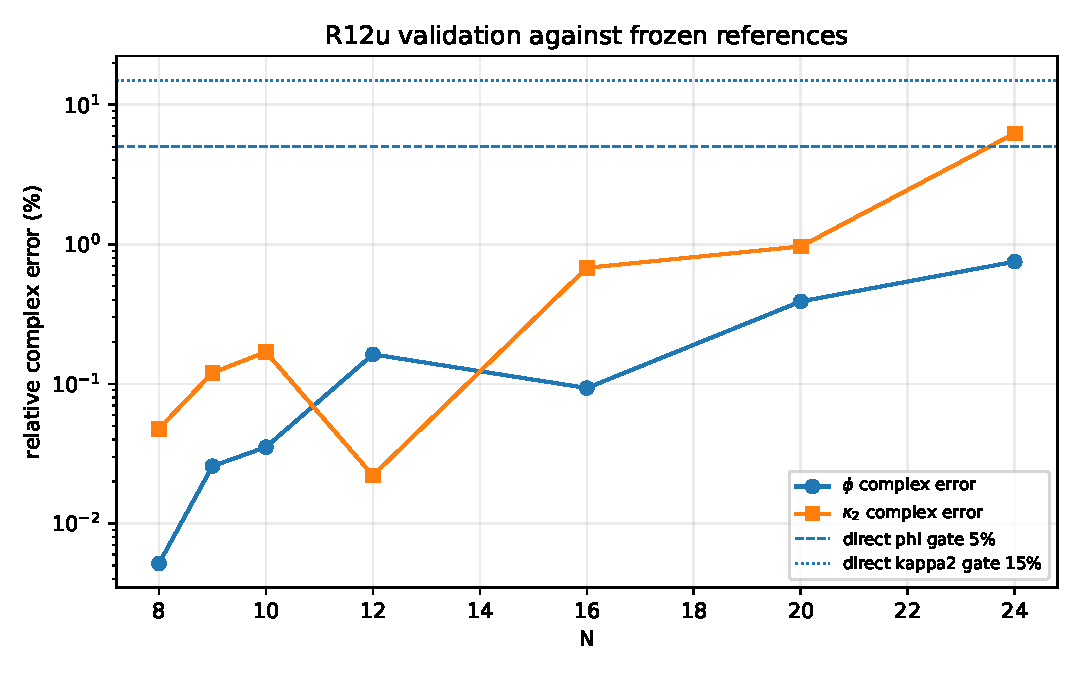
\includegraphics[width=0.76\textwidth]{r12u_validation_errors.pdf}
\caption{R12u. Errori complessi contro i riferimenti exact/direct congelati. Tutte le taglie di validazione superano i gate preregistrati.}
\end{figure}

La validazione completa autorizza quindi l'estensione $N=32,40,48,64$.

\subsection{Perdita della riduzione di varianza}

Il punto diagnostico piu netto non e un nuovo bias, ma la perdita progressiva di efficacia dei control variates. La mediana tra repliche del rapporto fra trace variance aggiustata e grezza e:
\begin{center}
\begin{tabular}{rccc}
\toprule
$N$ & $Y_0$ & $Y_1$ & $Y_2$ \\
\midrule
8  & $0.264$ & $0.282$ & $0.312$ \\
12 & $0.542$ & $0.550$ & $0.572$ \\
16 & $0.733$ & $0.737$ & $0.758$ \\
20 & $0.862$ & $0.860$ & $0.879$ \\
24 & $0.947$ & $0.940$ & $0.953$ \\
32 & $1.020$ & $1.015$ & $1.017$ \\
40 & $1.052$ & $1.051$ & $1.050$ \\
48 & $1.089$ & $1.089$ & $1.089$ \\
64 & $1.212$ & $1.213$ & $1.214$ \\
\bottomrule
\end{tabular}
\end{center}

\begin{figure}[htbp]
\centering
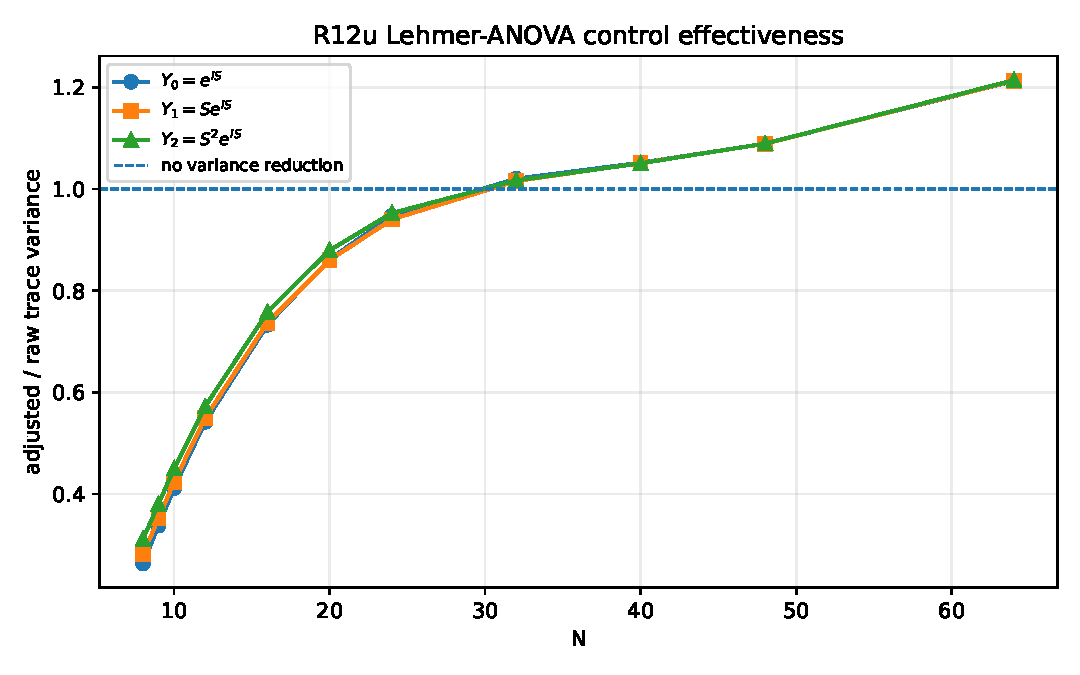
\includegraphics[width=0.76\textwidth]{r12u_variance_ratio.pdf}
\caption{R12u. Efficacia delle control variates di Lehmer. Il guadagno forte a piccole taglie decade con $N$ e scompare attorno a $N=32$; successivamente il rumore di training aggiunge una piccola penalita.}
\end{figure}

Coerentemente, nell'estensione soltanto una replica a $N=32$ supera il gate individuale di precisione su $\kappa_2$; a $N=40,48,64$ nessuna replica supera contemporaneamente i quality gate congelati. Il numero di repliche valide e quindi
\begin{equation}
 N=32:1/3,\qquad N=40:0/3,\qquad N=48:0/3,\qquad N=64:0/3.
\end{equation}

\begin{figure}[htbp]
\centering
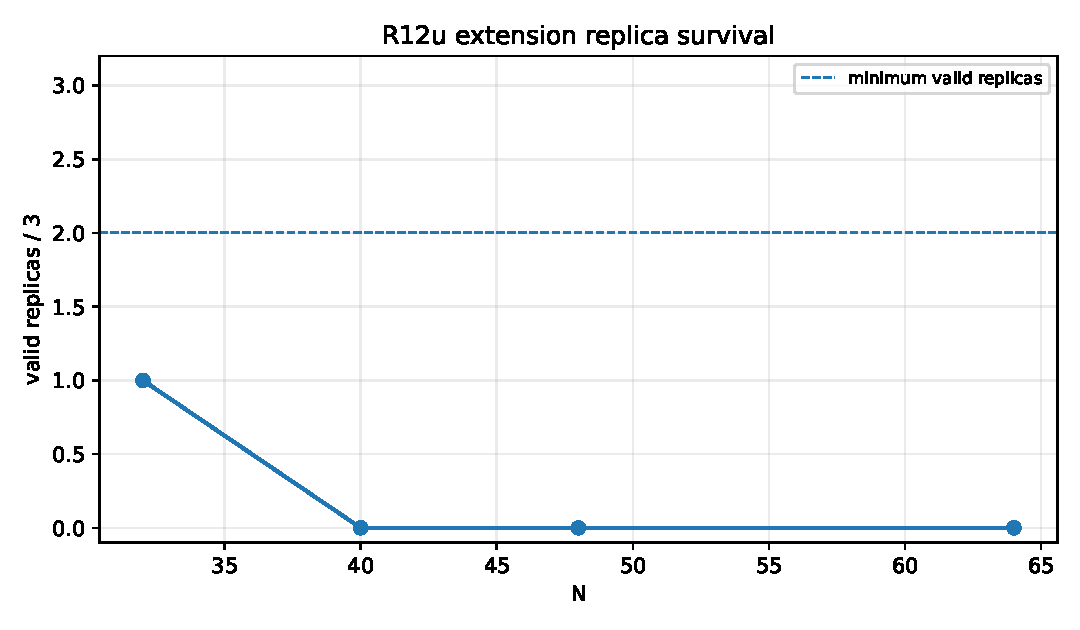
\includegraphics[width=0.68\textwidth]{r12u_replica_survival.pdf}
\caption{R12u extension. Numero di repliche che superano sia i gate interni sia la consistency rule. Il minimo preregistrato e due.}
\end{figure}

Il risultato mostra che il codice di Lehmer contiene informazione sufficiente a spiegare una larga frazione della varianza small-$N$, ma una ANOVA locale di ordine uno e due non segue la struttura oscillatoria globale quando $|\phi|$ collassa. Il controllo non modifica quindi la barriera asintotica del sign problem.

\subsection{Verdetto del Gate R12u}

\textbf{Gate R12u:}
\begin{quote}
\status{LEHMER-DIGIT MAIN EFFECTS AND ADJACENT-PAIR ANOVA CONTROLS HAVE EXACT ZERO MEAN UNDER THE UNIFORM PERMUTATION MEASURE AND PASS THE FULL R12n EXACT AND R12o DIRECT VALIDATION THROUGH $N=24$. HOWEVER THEIR VARIANCE-REDUCTION POWER DECREASES MONOTONICALLY WITH SYSTEM SIZE AND VANISHES BY $N\simeq32$. ONLY ONE OF THREE $N=32$ REPLICAS SURVIVES THE FROZEN $\kappa_2$ PRECISION GATE, AND NO REPLICA SURVIVES AT $N=40,48,64$. THE PREREGISTERED SCALING FIT IS THEREFORE FORBIDDEN. FINAL CLASSIFICATION:} \texttt{R12U\_FINITE\_SIZE\_OR\_PRECISION\_INCONCLUSIVE}.
\end{quote}

R12u chiude anche una possibilita concettuale: la dipendenza locale/additiva dai digit indipendenti puo essere rimossa senza bias, ma il residuo che domina a grandi $N$ e una cancellazione collettiva non catturata da main effects o coppie adiacenti. Prima di introdurre un'altra famiglia numerica, il successivo R12v dovra quantificare il costo minimo imposto dal sign problem per stimatori a misura positiva e derivare una efficiency frontier in funzione di $|\phi|$, cosi da stabilire quali classi di metodi possano realisticamente migliorare la scala raggiungibile.


\section{Gate R12v: cost law del sign problem ed efficiency frontier}

R12v non introduce un nuovo campionatore. E un audit analitico retrospettivo sui dati gia congelati di R12o--R12u, descritto in \texttt{R12V\_ANALYSIS\_PLAN.json}; non viene quindi presentato come una nuova preregistrazione statistica. L'obiettivo e separare il costo inevitabile del campionamento positivo diretto dalle inefficienze specifiche dei diversi algoritmi.

\subsection{Costo esatto dell'average phase nel campionamento diretto}

Sotto la misura uniforme representation-weighted poniamo
\begin{equation}
 Y=e^{iS},\qquad \phi=\mathbb E[Y],\qquad
 \widehat\phi_M=\frac1M\sum_{j=1}^{M}Y_j.
\end{equation}
Poiche $|Y|=1$, per campioni iid vale esattamente
\begin{equation}
 \mathbb E\!\left[|\widehat\phi_M-\phi|^2\right]
 =\frac{1-|\phi|^2}{M}.
 \label{eq:r12v_phi_mse}
\end{equation}
Di conseguenza il relative root-MSE e
\begin{equation}
 r_\phi(M)=\frac{\sqrt{1-|\phi|^2}}{\sqrt{M}\,|\phi|},
\end{equation}
mentre per ottenere $r_\phi\le\delta$ sono necessari
\begin{equation}
 \boxed{M\ge M_\phi(\delta)
 =\frac{1-|\phi|^2}{\delta^2|\phi|^2}.}
 \label{eq:r12v_phase_cost}
\end{equation}
Nel regime $|\phi|\ll1$ questo diventa il noto costo $M\sim(\delta^2|\phi|^2)^{-1}$. Tale legge e propria del phase estimator diretto; non e un lower bound universale su ogni possibile riformulazione del problema. Il carattere genericamente difficile del sign problem e noto anche sul piano della complessita computazionale, ma l'NP-hardness generica non esclude soluzioni strutturate per classi speciali di sistemi \cite{TroyerWiese2005,AlexandruEtAl2022}.

Il confronto con R12o e quasi parametrico: per $N=12$--$40$ il rapporto tra relative SE osservata a $10^6$ campioni e la previsione di Eq.~\eqref{eq:r12v_phi_mse} resta tra circa $0.83$ e $1.23$. Il collasso dell'average phase non e quindi un artefatto del codice R12o: il campionatore diretto sta gia operando vicino alla propria noise floor statistica.

\begin{figure}[htbp]
\centering
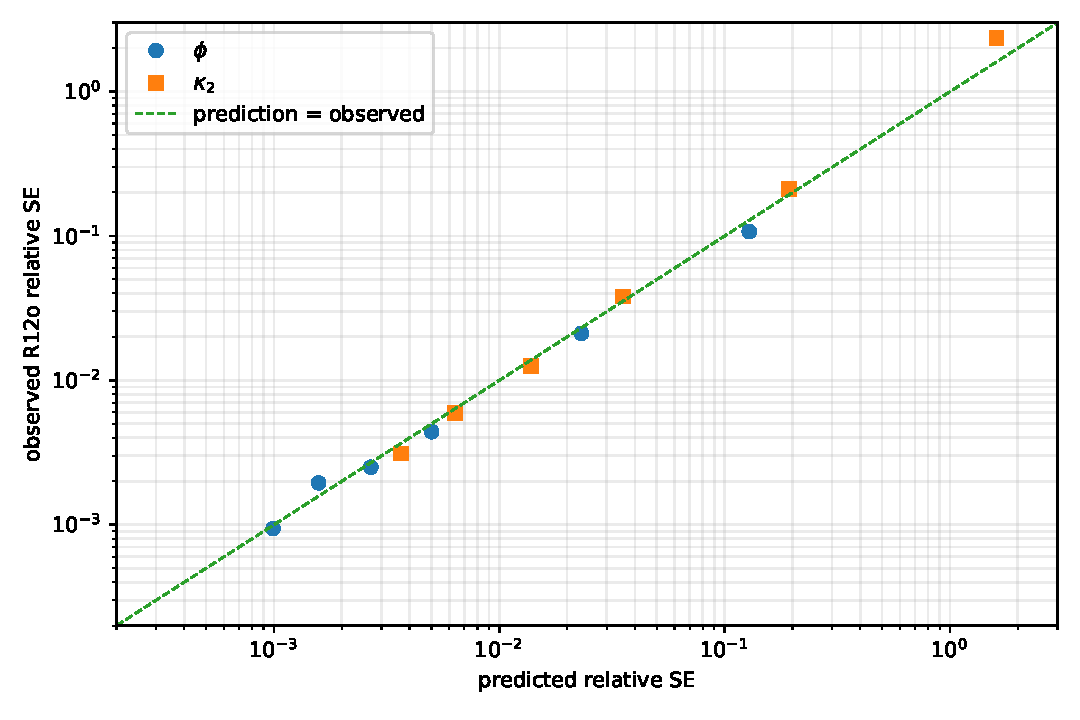
\includegraphics[width=0.78\textwidth]{r12v_prediction_check.pdf}
\caption{R12v. Errore relativo osservato in R12o contro quello previsto dalle formule analitiche. Per $\phi$ la relazione e esatta nel modello iid; per $\kappa_2$ viene usata la delta-method, affidabile finche il rapporto non entra nel regime fortemente non lineare.}
\end{figure}

\subsection{Amplificazione del secondo cumulante connesso}

Definiamo i momenti oscillanti
\begin{equation}
 z_r=\mathbb E[S^r e^{iS}],\qquad
 m=\frac{z_1}{z_0},\qquad
 \kappa_2=\frac{z_2}{z_0}-m^2,
 \qquad z_0=\phi.
\end{equation}
La linearizzazione del plug-in estimator fornisce l'influence variable
\begin{equation}
 \psi(S)=\frac{e^{iS}}{\phi}\left[(S-m)^2-\kappa_2\right],
 \qquad \mathbb E[\psi]=0,
 \label{eq:r12v_influence}
\end{equation}
cosicche, asintoticamente,
\begin{equation}
 \mathbb E|\widehat\kappa_2-\kappa_2|^2
 \simeq \frac{1}{M|\phi|^2}
 \mathbb E_0\!\left[\left|(S-m)^2-\kappa_2\right|^2\right].
 \label{eq:r12v_kappa_mse}
\end{equation}
Il denominatore $|\phi|^2$ compare quindi anche qui, moltiplicato da un shape factor che cresce con $N$. La delta-method riproduce l'incertezza R12o su $\kappa_2$ entro circa il $15\%$ relativo sul range $N=12$--$32$; a $N=40$ il plug-in estimator e ormai talmente rumoroso che la linearizzazione stessa entra nel regime non perturbativo.

La frontiera quantitativa e drastica. Per una precisione relativa del $5\%$ su $\phi$ e del $15\%$ su $\kappa_2$ il costo iid stimato e:
\begin{center}
\begin{tabular}{rrrr}
\toprule
$N$ & $|\phi|$ & $M_\phi(5\%)$ & $M_{\kappa_2}(15\%)$\\
\midrule
12 & 0.7100 & $3.94\times10^2$ & $5.95\times10^2$\\
16 & 0.5349 & $9.98\times10^2$ & $1.79\times10^3$\\
20 & 0.3481 & $2.90\times10^3$ & $8.53\times10^3$\\
24 & 0.1956 & $1.01\times10^4$ & $5.57\times10^4$\\
32 & 0.04313 & $2.15\times10^5$ & $1.66\times10^6$\\
40 & 0.007776 & $6.61\times10^6$ & $1.15\times10^8$\\
\bottomrule
\end{tabular}
\end{center}
Quindi il milione di campioni R12o e sufficiente per una buona misura di fase a $N=32$, ma e appena sotto il costo asintotico richiesto per un $15\%$ su $\kappa_2$; a $N=40$ il secondo cumulante richiede gia, nel modello diretto, dell'ordine di $10^8$ campioni efficaci.

\begin{figure}[htbp]
\centering
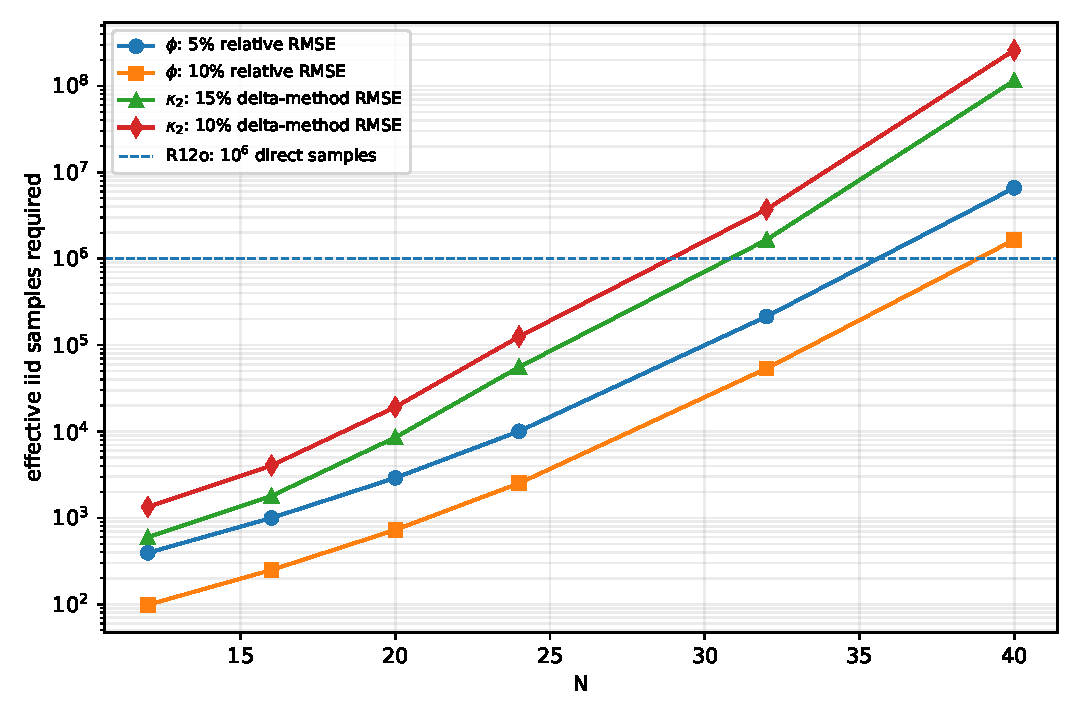
\includegraphics[width=0.78\textwidth]{r12v_cost_frontier.pdf}
\caption{R12v. Frontiera del numero di campioni iid necessario sotto la misura positiva uniforme. Il costo di $\kappa_2$ cresce piu rapidamente della sola misura della fase. La linea orizzontale indica il budget di $10^6$ campioni di R12o.}
\end{figure}

\subsection{Perche la fase decade: quasi-Gaussianita della DOS sul range risolto}

La cumulant expansion ordinaria implica
\begin{equation}
 \Re\log\phi(1)=-\frac{\mathrm{Var}_0(S)}2+\frac{\kappa_4^{(0)}}{24}-\cdots.
\end{equation}
Definiamo pertanto
\begin{equation}
 G_N=\frac{-2\log|\phi_N(1)|}{\mathrm{Var}_0(S)}.
\end{equation}
Sul range primario $N=12$--$40$ si trova
\begin{equation}
 \boxed{0.89\lesssim G_N\lesssim0.98.}
\end{equation}
La severita del sign problem e quindi gia spiegata in larga misura dal secondo cumulante ordinario della distribuzione positiva dell'azione; le correzioni non gaussiane sono visibili ma non dominanti nel range ancora risolto.

\begin{figure}[htbp]
\centering
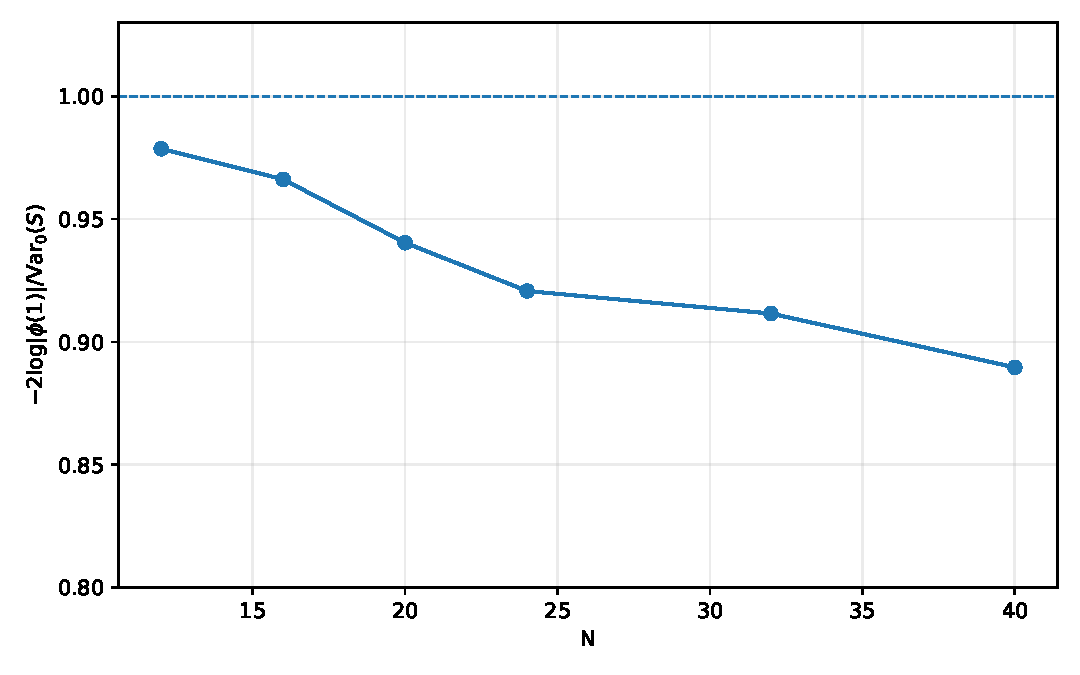
\includegraphics[width=0.72\textwidth]{r12v_gaussian_diagnostic.pdf}
\caption{R12v. Diagnostica quasi-gaussiana. Il rapporto $-2\log|\phi|/\mathrm{Var}_0(S)$ resta vicino a uno fino a $N=40$, indicando che la varianza ordinaria dell'azione controlla gran parte della perdita di fase.}
\end{figure}

R12m aveva gia trovato, sul range piu lungo $N=24$--$96$, uno scaling fixed-$N$
\begin{equation}
 \mathrm{Var}_0(S)\propto N^{1.8574}.
\end{equation}
Se -- e soltanto se -- la quasi-gaussianita osservata sopra restasse di ordine uno asintoticamente, ne seguirebbe la conseguenza condizionale
\begin{equation}
 -\log|\phi|=O(N^{1.8574}),\qquad
 M_{\rm crude}=\exp[O(N^{1.8574})].
 \label{eq:r12v_conditional_cost}
\end{equation}
Questa non e una legge asintotica misurata: combina due regimi numerici diversi e viene registrata esclusivamente come implicazione condizionale da testare.

\subsection{Lettura della frontiera R12o--R12u}

La frontiera chiarisce i risultati precedenti. R12o a $N=32$ usa $10^6$ campioni, contro una richiesta delta-method di circa $1.66\times10^6$ per un $15\%$ su $\kappa_2$: il fallimento marginale era quantitativamente atteso. R12t riesce a oltrepassare $N=24$ e conserva due repliche a $N=32$, ma non produce una riduzione di ordine parametrico; R12u mostra direttamente che il fattore di variance reduction tende a uno attorno alla stessa taglia. A $N=40$ una strategia direct-like richiederebbe gia circa $1.15\times10^8$ campioni efficaci per lo stesso target su $\kappa_2$, molto oltre i budget usati finora.

Ne segue un criterio operativo: un nuovo algoritmo e interessante per l'estensione soltanto se modifica almeno una delle tre quantita seguenti in modo crescente con $N$:
\begin{enumerate}
\item la magnitudine residua dell'average phase nella nuova rappresentazione;
\item il fattore di varianza dell'influence variable di Eq.~\eqref{eq:r12v_influence};
\item il costo per campione in modo sufficiente da compensare la crescita richiesta di $M$.
\end{enumerate}
Una riduzione di varianza con fattore costante non puo cambiare la classe di costo se $|\phi|$ continua a collassare.

\subsection{Verdetto del Gate R12v}

\textbf{Gate R12v:}
\begin{quote}
\status{FOR THE DIRECT POSITIVE-MEASURE ESTIMATOR THE AVERAGE-PHASE RELATIVE MSE IS EXACTLY $(1-|\phi|^2)/(M|\phi|^2)$, AND R12o SATURATES THIS LAW TO WITHIN ORDINARY FINITE-SAMPLE FLUCTUATIONS. THE DELTA-METHOD INFLUENCE FUNCTION FOR $\kappa_2$ EXPLAINS THE OBSERVED ERROR GROWTH THROUGH $N=32$ AND PREDICTS AN $O(10^8)$ EFFECTIVE-SAMPLE REQUIREMENT ALREADY AT $N=40$ FOR 15\% RELATIVE PRECISION. THE RESOLVED DOS IS NEAR-GAUSSIAN IN THE SENSE $-2\log|\phi|/\mathrm{Var}_0(S)\simeq0.89$--$0.98$. THESE RESULTS DEFINE A CLASS-RESTRICTED EFFICIENCY FRONTIER, NOT AN ALGORITHM-INDEPENDENT NO-GO: STRUCTURED REPRESENTATION CHANGES CAN IN PRINCIPLE ALTER THE PHASE OR THE INFLUENCE VARIANCE. NO SUCH ASYMPTOTIC ESCAPE HAS YET BEEN DERIVED FOR THIS BENCHMARK. FINAL CLASSIFICATION:} \texttt{DIRECT\_COST\_LAW\_DERIVED\_NO\_ASYMPTOTIC\_ESCAPE\_DERIVED}.
\end{quote}

R12v cambia quindi la strategia: oltre $N\simeq32$ non e razionale continuare soltanto ad aumentare moderatamente la statistica o aggiungere control variates locali. Il Gate R12w cerca quindi una struttura analitica della density of states -- large deviations, saddle point o altra rappresentazione -- capace di calcolare direttamente la trasformata oscillante senza pagare il costo $|\phi|^{-2}$ del phase estimator positivo.

\section{Gate R12w: scaled density, large-deviation structure e finestra saddle}

\subsection{Integrita del test e surrogate massimo-entropia troncato}

La forma del modello di densita e stata scelta durante development usando i risultati storici gia disponibili R12n--R12v; per questo motivo tali dati non vengono riutilizzati come ``validazione cieca''. Il file \texttt{R12W\_ANALYSIS\_PLAN.json}, congelato prima della nuova produzione, specifica un holdout completamente nuovo: tre stream uniformi indipendenti da $250\,000$ permutazioni ciascuno per
\begin{equation}
N=8,9,10,12,16,20,24,32,40,48,64,
\end{equation}
con seed non usati nei gate precedenti. Exact $N=8$--$10$ viene confrontato con R12n; $N=12$--$24$ viene confrontato con gli stream diretti indipendenti R12o. L'estensione $N=32$--$64$ usa R12o soltanto nei punti $(N,g)$ in cui l'incertezza del riferimento rimane preregistratamente controllata.

Il modello scelto in R12w era un surrogate massimo-entropia per la variabile standardizzata
\begin{equation}
z=\frac{S-\mu_N}{\sigma_N},
\end{equation}
che riproduce esattamente i primi sei momenti standardizzati del nuovo holdout:
\begin{equation}
 p_6(z)=\frac{1}{\mathcal Z_6}\exp\!\left(a_1z+a_2z^2+a_3z^3+a_4z^4+a_5z^5-e^{\eta}z^6\right).
 \label{eq:r12w_maxent}
\end{equation}
Il termine sestico negativo rende normalizzabile la continuazione formale del polinomio esponenziale. Tuttavia, come auditato retroattivamente in R12x, l'implementazione numerica R12w determinava momenti, normalizzazione e trasformata con quadratura Gauss--Legendre sulla finestra finita $z\in[-10,10]$. Pertanto il replay R12w valida un surrogate reale troncato, non una densita globale identificata. I parametri non vengono fittati alla characteristic function: sono determinati unicamente dai momenti reali della misura positiva. Una volta ottenuta $p_6$, la trasformata oscillante e i due momenti complessi vengono calcolati per quadratura deterministica, senza troncamento Taylor in $g$:
\begin{align}
 \phi_6(g)&=e^{ig\mu_N}\int_{-10}^{10} dz\,p_6(z)e^{ig\sigma_Nz},\\
 \kappa_{2,6}(g)&=\sigma_N^2\left[\frac{\int_{-10}^{10} dz\,z^2p_6(z)e^{ig\sigma_Nz}}{\int_{-10}^{10} dz\,p_6(z)e^{ig\sigma_Nz}}-
 \left(\frac{\int_{-10}^{10} dz\,zp_6(z)e^{ig\sigma_Nz}}{\int_{-10}^{10} dz\,p_6(z)e^{ig\sigma_Nz}}\right)^2\right].
 \label{eq:r12w_fourier}
\end{align}
Questa costruzione e vicina concettualmente alle tecniche saddlepoint/steepest-descent, che cercano di sostituire una espansione locale dei momenti con una approssimazione globale della densita o del cumulant-generating function \cite{Daniels1954,LundeKleppeSkaug2018}. Non viene tuttavia assunta alcuna validita asintotica a priori.

\subsection{Exact e direct holdout validation}

Le soglie congelate a $g=1$ sono $1\%/10\%$ su $\phi/\kappa_2$ per exact $N=8$--$10$ e $2\%/15\%$ per direct $N=12$--$24$. Tutte le taglie passano:
\begin{center}
\begin{tabular}{rccc}
\toprule
$N$ & riferimento & errore complesso $\phi$ & errore complesso $\kappa_2$\\
\midrule
8  & exact  & $0.078\%$ & $0.204\%$\\
9  & exact  & $0.047\%$ & $1.129\%$\\
10 & exact  & $0.091\%$ & $1.186\%$\\
12 & direct & $0.112\%$ & $0.632\%$\\
16 & direct & $0.056\%$ & $1.441\%$\\
20 & direct & $0.530\%$ & $3.103\%$\\
24 & direct & $0.738\%$ & $13.492\%$\\
\bottomrule
\end{tabular}
\end{center}
Il surrogate sestico troncato supera quindi il punto $N=24$ in cui la serie cumulante R12p aveva perso convergenza: la differenza e che Eq.~\eqref{eq:r12w_maxent}, sulla finestra implementata, ricostruisce una misura positiva normalizzata e la integra non perturbativamente in $g$, invece di valutare un polinomio troncato per $\log\phi$.

\subsection{Una legge di scala inattesa: $X_N=(S-4)/N$}

Il nuovo holdout mostra una struttura molto piu forte di una semplice ``quasi-gaussianita''. Nel range $N=24$--$64$,
\begin{equation}
 \boxed{\mathrm{Var}_0(S)=A N^{\gamma_S},\qquad
 \gamma_S=2.00395,\quad A=0.0064021,\quad R^2_{\log}=0.9956.}
 \label{eq:r12w_varN2}
\end{equation}
Inoltre $\langle S\rangle$ tende rapidamente al valore circa $4$ gia noto per il benchmark random-order 2d. E quindi naturale introdurre
\begin{equation}
 \boxed{X_N=\frac{S-4}{N}.}
 \label{eq:r12w_scaledX}
\end{equation}
La sua varianza resta dell'ordine $6\times10^{-3}$ e le distanze Kolmogorov--Smirnov fra distribuzioni consecutive $N=24,32,40,48,64$ sono soltanto
\begin{equation}
0.0181,\quad0.0071,\quad0.0075,\quad0.0136.
\end{equation}
Quindi, sul range misurato, la DOS positiva non presenta la classica concentrazione di una variabile estensiva con fluttuazioni $O(\sqrt N)$: presenta piuttosto una forma larga quasi collassante per $X_N$. Contemporaneamente l'excess kurtosis diminuisce approssimativamente come
\begin{equation}
 \gamma_2(X_N)\sim6.32\,N^{-0.976},
\end{equation}
quindi la forma standardizzata si avvicina lentamente a una gaussiana pur mantenendo una larghezza di $S$ circa proporzionale a $N$.

\begin{figure}[htbp]
\centering
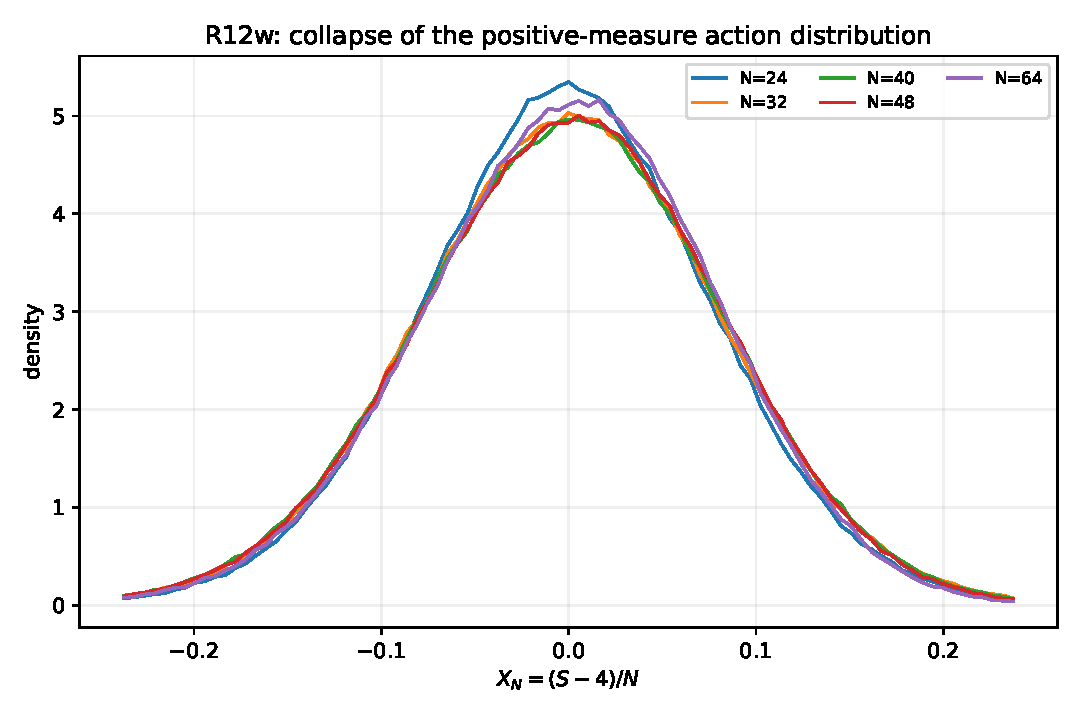
\includegraphics[width=0.88\textwidth]{r12w_scaled_density_collapse.pdf}
\caption{R12w. Nuovi holdout indipendenti: densita della variabile scalata $X_N=(S-4)/N$. La quasi-sovrapposizione delle curve e quantificata dai piccoli KS consecutivi.}
\end{figure}

\begin{figure}[htbp]
\centering
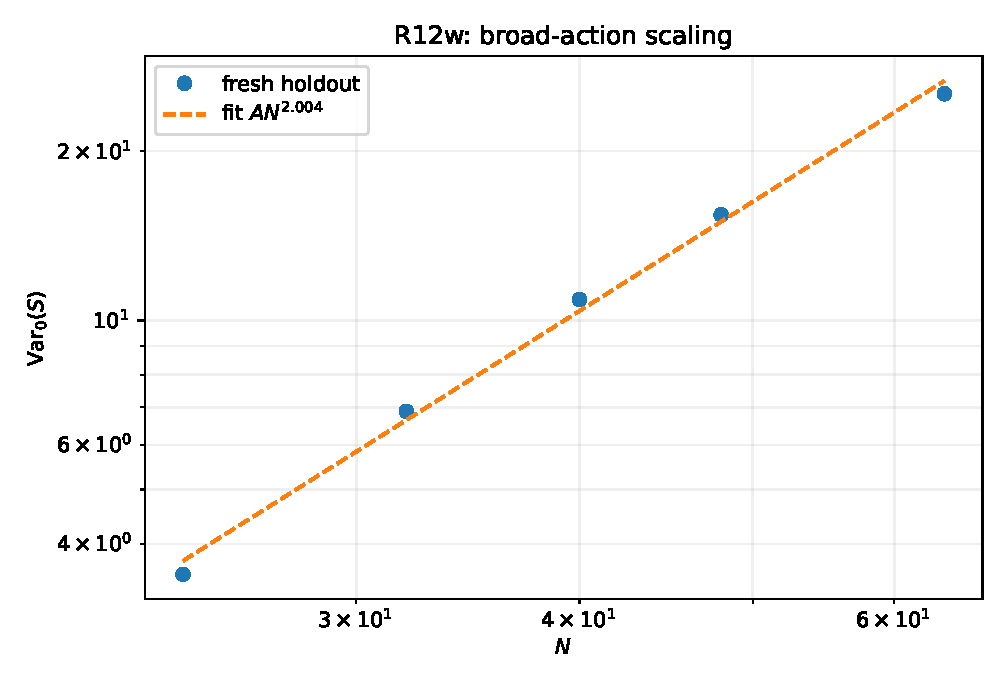
\includegraphics[width=0.72\textwidth]{r12w_variance_scaling.pdf}
\caption{R12w. Scaling della varianza positiva dell'azione. Sul range $N=24$--$64$ il fit e praticamente quadratico, $\gamma_S=2.004$. Non viene assunto che questo esponente sia gia asintotico.}
\end{figure}

\subsection{Il sign problem come trasformata ad alta frequenza}

La definizione \eqref{eq:r12w_scaledX} produce una identita esatta, indipendente dal modello sestico:
\begin{equation}
 \boxed{\phi_N(g)=\mathbb E[e^{igS}]=e^{4ig}\,\mathbb E[e^{i(gN)X_N}]
       =e^{4ig}\,\widehat f_N(gN),}
 \label{eq:r12w_highfreq}
\end{equation}
con $f_N$ densita (o misura) di $X_N$. Se $f_N$ converge a una densita integrabile non banale, il lemma di Riemann--Lebesgue implica qualitativamente $\widehat f_N(gN)\to0$ a frequenza crescente; il tasso dipende dalla regolarita e dalla struttura analitica di $f_N$. Nel limite esattamente gaussiano con $\mathrm{Var}(X_N)=A$,
\begin{equation}
 |\phi_N(g)|=\exp\!\left(-\frac12 A g^2N^2\right),
 \label{eq:r12w_gaussianN2}
\end{equation}
che e precisamente la forma suggerita dalla diagnostica quasi-gaussiana di R12v. La cost law $|\phi|^{-2}$ diventerebbe allora $\exp(A g^2N^2)$, ma Eq.~\eqref{eq:r12w_gaussianN2} resta una conseguenza condizionale della persistenza del regime osservato, non una legge asintotica dimostrata.

Questa riscrittura chiarisce perche i cumulanti locali possono essere accurati vicino a $g=0$ e fallire al target. Il parametro che controlla la trasformata della densita standardizzata non e $g$ da solo ma
\begin{equation}
 t=g\sigma_N.
 \label{eq:r12w_t}
\end{equation}
Poiche $\sigma_N\simeq\sqrt{A}\,N$ sul range corrente, il punto fisico $g=1$ si sposta linearmente verso frequenze standardizzate sempre maggiori.

\subsection{Finestra Fourier/saddle empiricamente validata}

Nell'estensione R12w il modello non viene giudicato contro riferimenti R12o non risolti. Un punto $(N,g)$ e utilizzabile soltanto se il riferimento diretto ha errore relativo preregistrato inferiore a $5\%$ per $\phi$ e $20\%$ per $\kappa_2$; il modello deve poi restare entro $5\%/20\%$ dal riferimento. La massima frequenza standardizzata che supera entrambi i controlli e
\begin{center}
\begin{tabular}{rcc}
\toprule
$N$ & $t_{\max}=g\sigma_N$ validato & $t(g=1)=\sigma_N$\\
\midrule
32 & 1.968 & 2.624\\
40 & 1.650 & 3.299\\
48 & 1.961 & 3.923\\
64 & 2.513 & 5.026\\
\bottomrule
\end{tabular}
\end{center}
La mediana della frontiera e
\begin{equation}
 \boxed{t_*\simeq1.965.}
\end{equation}
A $N=32$ il modello e ancora validato a $g=0.75$ ma non dispone di un riferimento $g=1$ sufficientemente preciso; a $N=40$ il primo fallimento controllabile compare gia a $g=0.75$, mentre a $N=48$--$64$ soltanto frequenze piu basse restano direttamente verificabili.

\begin{figure}[H]
\centering
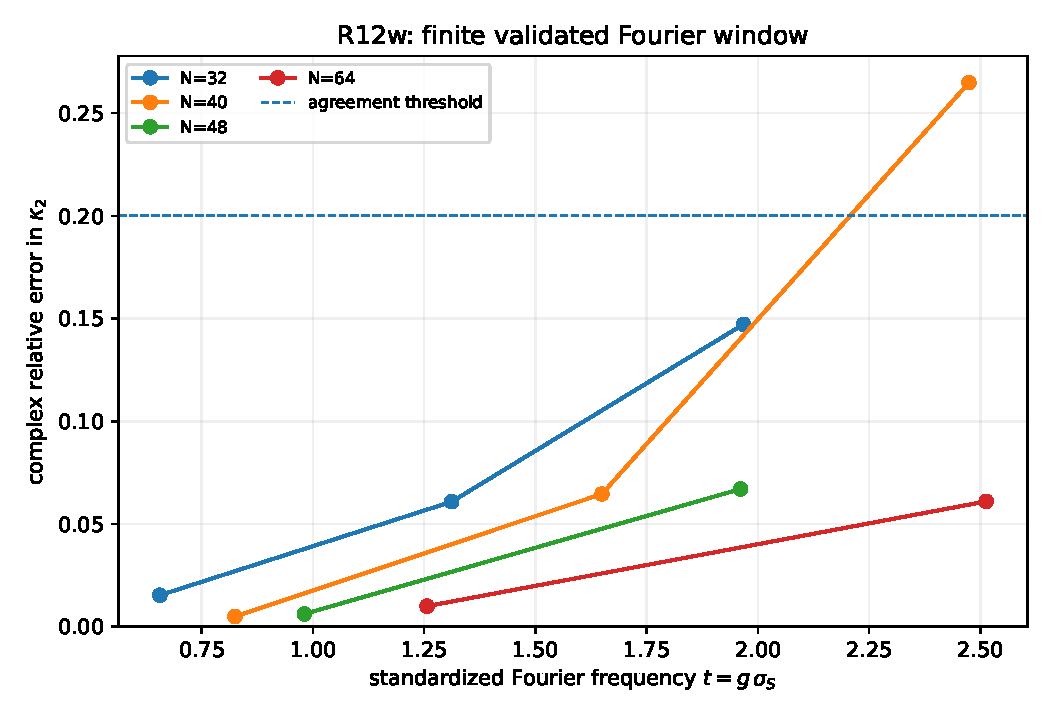
\includegraphics[width=0.82\textwidth]{r12w_frequency_frontier.pdf}
\caption{R12w. Errore del cumulante del modello sestico contro la frequenza standardizzata $t=g\sigma_S$ nei soli punti con riferimento direct-MC sufficientemente risolto. La soglia preregistrata e $20\%$. La finestra validata resta $t=O(2)$, mentre $g=1$ porta $t$ crescente con $N$.}
\end{figure}

La continuazione \emph{formale} del polinomio in Eq.~\eqref{eq:r12w_maxent} permette di scrivere l'equazione
\begin{equation}
 a_1+2a_2z_*+3a_3z_*^2+4a_4z_*^3+5a_5z_*^4-6e^\eta z_*^5+it=0.
 \label{eq:r12w_saddle}
\end{equation}
R12w usava questa equazione soltanto come motivazione per il gate successivo, non come dato numerico di classificazione. L'audit R12x mostra ora che la continuazione globale del polinomio non e identificata dal fit sulla finestra: in alcune repliche compaiono modi remoti dominanti che la quadratura $[-10,10]$ non vede. Di conseguenza Eq.~\eqref{eq:r12w_saddle} non puo essere interpretata come equazione dei saddle fisici della DOS. Resta invece valido il risultato empirico della finestra Fourier reale e l'identita esatta \eqref{eq:r12w_highfreq}. La letteratura saddlepoint conferma che una deformazione complessa richiede controllo della funzione generatrice/contorno globale, non il semplice matching di pochi momenti \cite{Daniels1954,LundeKleppeSkaug2018}.

\subsection{Verdetto del Gate R12w}

\textbf{Gate R12w, interpretazione corretta da R12x:}
\begin{quote}
\status{IL FRESH HOLDOUT CONFERMA $\mathrm{Var}(S)\propto N^{2.004}$, IL QUASI-COLLASSO DI $X_N=(S-4)/N$ E L'IDENTITA ESATTA $\phi_N(g)=e^{4ig}\widehat f_N(gN)$. IL SURROGATE SESTICO TRONCATO USATO NELL'IMPLEMENTAZIONE PASSA EXACT $N=8$--$10$ E DIRECT $N=12$--$24$ E DEFINISCE UNA FINESTRA FOURIER EMPIRICAMENTE VALIDATA $t=g\sigma_S=O(2)$. R12x MOSTRA PERO CHE LA SUA CONTINUAZIONE SU TUTTA $\mathbb R$ NON E UNA DENSITA GLOBALE IDENTIFICATA. PERTANTO RESTANO VALIDI I RISULTATI REAL-AXIS/FREQUENCY-WINDOW, MENTRE VIENE RITIRATA QUALUNQUE INTERPRETAZIONE DEI SADDLE DEL SESTICO COME SADDLE FISICI DELLA DOS.}
\end{quote}

Lo status storico \texttt{R12W\_RATE\_MODEL\_VALIDATED\_LOCAL\_FOURIER\_WINDOW\_NO\_G1\_ESCAPE} viene conservato nei file di audit, ma in v0.28 e scientificamente reinterpretato come ``local truncated surrogate validated / no $g=1$ escape''. R13 resta bloccato.


\section{Gate R12x: audit della continuazione complessa}

\subsection{Perche il saddle del sestico non era ancora autorizzato}

R12x parte da un controllo retroattivo della premessa necessaria per una analisi di steepest descent: la funzione reale fittata deve essere una rappresentazione globale coerente della misura positiva, non soltanto un interpolante accurato nella regione in cui e stata integrata. Il codice R12w utilizzava $500$ nodi Gauss--Legendre sulla finestra
\begin{equation}
 z\in[-10,10]
\end{equation}
per il matching dei momenti e per le trasformate. Il polinomio esponenziale aveva un coefficiente sestico negativo, ma i coefficienti erano quindi selezionati rispetto alla misura \emph{troncata}. Estendere successivamente lo stesso polinomio su tutta $\mathbb R$ costituisce una ipotesi nuova.

L'audit deterministico \texttt{R12X\_GLOBAL\_SURROGATE\_AUDIT.json} calcola tutte le radici reali di $P'(z)$, con
\begin{equation}
 P(z)=a_1z+a_2z^2+a_3z^3+a_4z^4+a_5z^5-e^\eta z^6,
\end{equation}
e confronta ogni massimo reale con quello centrale. In $9$ delle $33$ repliche compare un massimo globale remoto fuori da $|z|=10$. Il problema non riguarda soltanto le taglie grandi: a $N=8$ accade in $3/3$ repliche, con un caso in cui il massimo remoto supera quello centrale di oltre $6\times10^6$ in $\log p$; a $N=32$ accade ancora in $3/3$ repliche, con $\Delta\log p$ fino a circa $64$, a $N=40$ in $2/3$ e a $N=64$ in $1/3$.

\begin{figure}[H]
\centering
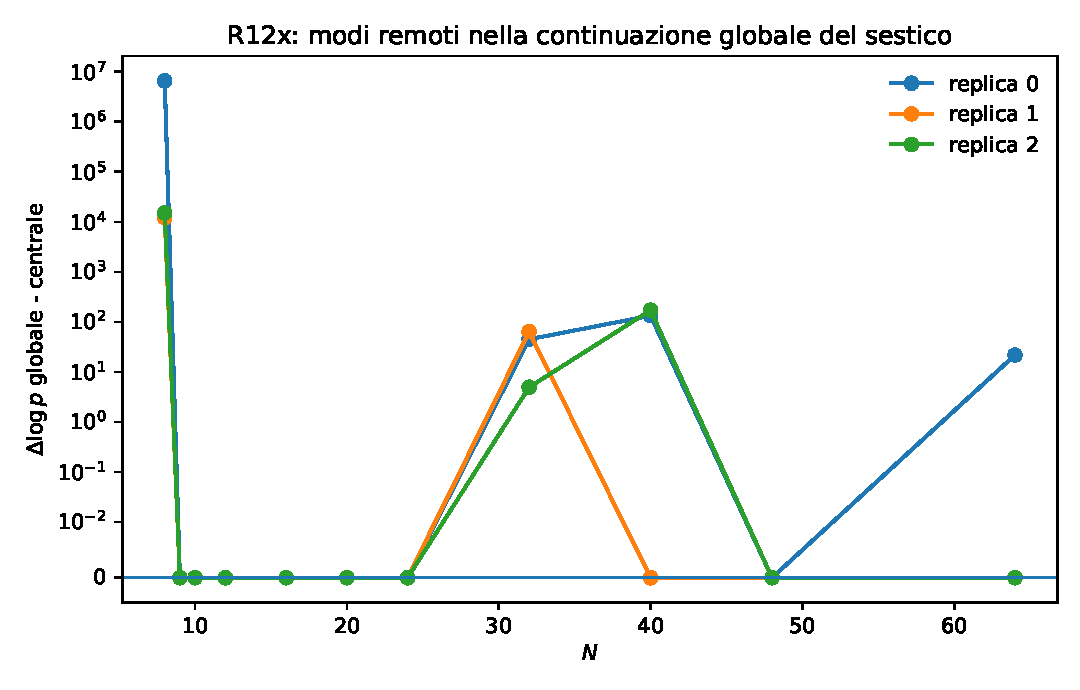
\includegraphics[width=0.82\textwidth]{r12x_global_surrogate_audit.pdf}
\caption{R12x. Differenza fra il massimo globale della continuazione del sestico e il massimo centrale usato dal surrogate troncato. Valori positivi con modo remoto mostrano che il fit R12w non puo essere reinterpretato come densita globale su $\mathbb R$. La scala verticale e simmetrico-logaritmica.}
\end{figure}

Il fatto che R12w passi exact/direct non e in contraddizione: quei test verificano precisamente la mappa numerica implementata sulla finestra $[-10,10]$. Non verificano la massa che la continuazione formale assegnerebbe a regioni mai integrate. La classificazione numerica R12w resta quindi utile come \emph{surrogate locale di Fourier}; viene ritirata l'etichetta ``global rate model''.

\subsection{Sei momenti non identificano la fase ad alta frequenza}

Il problema e piu generale del particolare sestico. Un numero finito di momenti definisce un problema dei momenti troncato e, salvo casi speciali, non seleziona un'unica misura positiva \cite{CurtoFialkow1991}. Per quantificare l'effetto esattamente sul nostro target, R12x prende per ciascun $N$ i momenti standardizzati
\begin{equation}
 m_k=\mathbb E[z^k],\qquad k=0,\ldots,6,
\end{equation}
misurati nei nuovi holdout R12w. Su una griglia di $1601$ quantili compresa \emph{interamente nel supporto osservato}, vengono poi risolti quattro programmi lineari positivi: massimo/minimo della parte reale e della parte immaginaria di
\begin{equation}
 \varphi(t)=\int e^{itz}d\mu(z),\qquad t=\sigma_S\quad(g=1),
\end{equation}
soggetti a \emph{gli stessi} sette vincoli $m_0,\ldots,m_6$. I residui massimi dei vincoli sono $<3\times10^{-11}$.

\begin{center}
\begin{tabular}{rcc}
\toprule
$N$ & intervallo ammesso per $\Re\varphi$ & intervallo ammesso per $\Im\varphi$\\
\midrule
24 & $[0.118,\ 0.353]$ & $[-0.161,\ 0.126]$\\
32 & $[-0.313,\ 0.575]$ & $[-0.529,\ 0.476]$\\
40 & $[-0.772,\ 0.931]$ & $[-0.907,\ 0.851]$\\
48 & $[-0.981,\ 1.000]$ & $[-0.994,\ 0.993]$\\
64 & $[-1.000,\ 1.000]$ & $[-1.000,\ 1.000]$\\
\bottomrule
\end{tabular}
\end{center}

\begin{figure}[H]
\centering
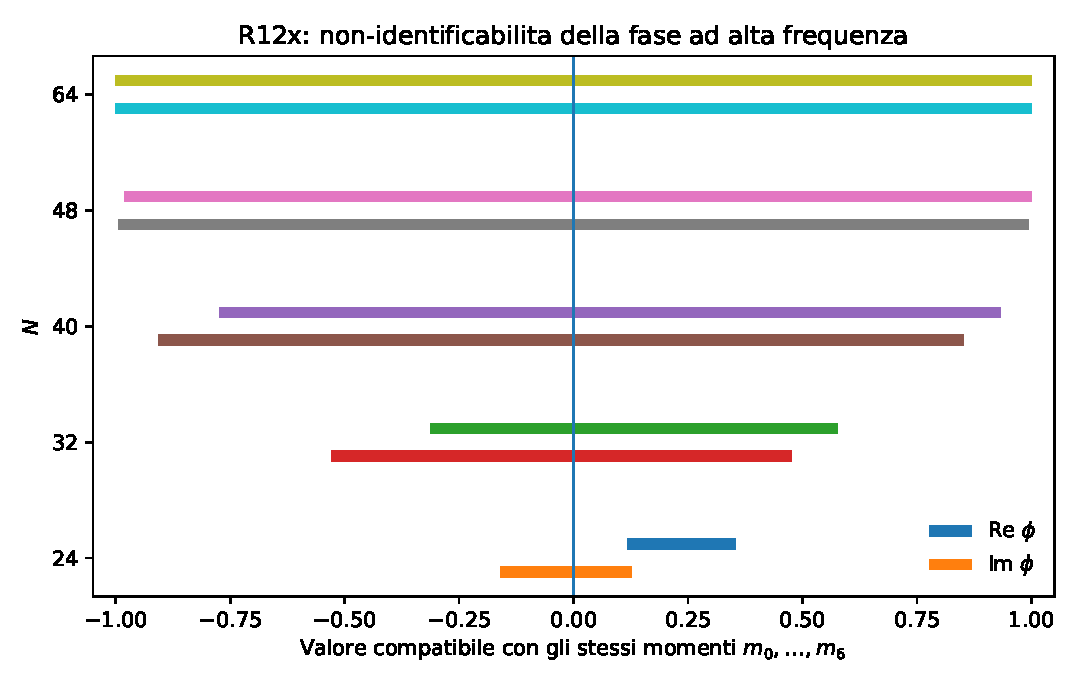
\includegraphics[width=0.82\textwidth]{r12x_moment_nonidentifiability.pdf}
\caption{R12x. Intervalli estremi della parte reale e immaginaria della characteristic function compatibili con gli stessi primi sei momenti e con supporto limitato all'intervallo osservato. A frequenza crescente il problema dei momenti diventa praticamente non informativo sul target complesso.}
\end{figure}

Questo e un no-go metodologico specifico ma forte: non basta aumentare l'accuratezza del fit dei sei momenti. Gia a $N=48$--$64$ esistono misure positive, sullo stesso intervallo reale e con gli stessi momenti fino al sesto ordine, le cui fasi ad alta frequenza occupano quasi tutto il disco consentito componente per componente. Di conseguenza anche la posizione e la dominanza dei saddle complessi non sono identificabili da R12w.

\subsection{Cosa sopravvive di R12w}

R12x non annulla i risultati strutturali ottenuti direttamente dai campioni. Restano acquisiti sul range misurato:
\begin{align}
 \mathrm{Var}(S)&\simeq0.006402\,N^{2.00395},\\
 X_N&=(S-4)/N\quad\text{con quasi-collasso empirico},\\
 \phi_N(g)&=e^{4ig}\widehat f_N(gN),
\end{align}
oltre alla finestra reale in cui il surrogate troncato riproduce exact/direct. Vengono invece esplicitamente ritirati come non autorizzati:
\begin{enumerate}
\item l'interpretazione di Eq.~\eqref{eq:r12w_maxent} come densita massimo-entropia globale su $\mathbb R$;
\item l'uso delle radici di Eq.~\eqref{eq:r12w_saddle} come saddle fisici della DOS;
\item qualunque inferenza di linee di Stokes dal solo matching $m_0,\ldots,m_6$.
\end{enumerate}

\subsection{La strada successiva: permutons invece di un'analiticita inventata}

Il benchmark 2d usato da R12n--R12x e una permutazione uniforme vista come ordine bidimensionale. Per le permutazioni casuali esiste una teoria large-deviation direttamente sullo spazio dei \emph{permutons}: la misura empirica soddisfa una LDP a velocita $N$ con rate function entropica, e i modelli esponenzialmente inclinati possono essere trattati tramite principi variazionali \cite{BorgaEtAl2024,KenyonEtAl2020}. Questo fornisce una possibile via meno arbitraria alla struttura saddle.

Il punto non ancora dimostrato e se l'azione BD/BDG del nostro benchmark ammetta, dopo la corretta riscalatura, una rappresentazione continua
\begin{equation}
 \frac{S_N-4}{N}\longrightarrow \mathcal A[\gamma]
 \label{eq:r12x_permuton_action}
\end{equation}
come funzionale di un permuton $\gamma$. Se esistesse una tale $\mathcal A$ sufficientemente regolare, il path sum oscillante avrebbe formalmente una struttura variazionale del tipo
\begin{equation}
 Z_N(g)\sim\int \mathcal D\gamma\,
 \exp\left\{N\left[H(\gamma)+ig\mathcal A(\gamma)\right]\right\},
 \label{eq:r12x_permuton_saddle}
\end{equation}
e i saddle complessi emergerebbero dall'oggetto combinatorio corretto invece che dalla continuazione arbitraria di sei momenti. Ma Eq.~\eqref{eq:r12x_permuton_action} e al momento soltanto il nuovo problema da testare: i conteggi di intervalli BDG possono dipendere da informazione microscopica piu fine della topologia dei permutons.

\subsection{Verdetto del Gate R12x}

\textbf{Gate R12x:}
\begin{quote}
\status{THE GLOBAL ANALYTIC CONTINUATION OF THE R12W SEXTIC SURROGATE IS NOT IDENTIFIED. NINE OF THIRTY-THREE FITS DEVELOP REMOTE DOMINANT REAL MODES OUTSIDE THE IMPLEMENTED QUADRATURE WINDOW, AND SIX MOMENTS ALONE ALLOW ALMOST ARBITRARY HIGH-FREQUENCY CHARACTERISTIC-FUNCTION COMPONENTS EVEN ON THE OBSERVED SUPPORT. THEREFORE A PHYSICAL COMPLEX-SADDLE/STOKES TOPOLOGY CANNOT BE INFERRED FROM R12W. THE REAL-AXIS SCALING RESULTS AND THE EXACT HIGH-FREQUENCY IDENTITY SURVIVE; THE GLOBAL-MAXENT/SADDLE INTERPRETATION IS WITHDRAWN. FINAL CLASSIFICATION:} \nolinkurl{R12X_GLOBAL_ANALYTIC_CONTINUATION_NOT_IDENTIFIED_STOKES_ANALYSIS_NOT_AUTHORIZED}.
\end{quote}

Questa era la domanda formulata alla chiusura storica di v0.28. Il Gate R12y della Sez.~\ref{sec:r12y} ha ora escluso un funzionale globale dipendente dal solo permuton e sposta il test sulla microstruttura degli intervalli. R13 resta bloccato.

\section{Gate R12y: il permuton non determina da solo l'azione BD a scala $N$}
\label{sec:r12y}

Il Gate R12x aveva proposto di cercare un limite funzionale $\mathcal A[\gamma]$ nello spazio dei permutons, al posto della continuazione complessa non giustificata del sestico. R12y verifica \emph{prima} il prerequisito deterministico di tale costruzione: se due successioni di permutazioni convergono allo stesso permuton $\gamma$, l'azione riscalata deve convergere allo stesso valore perche essa possa essere rappresentata da un unico funzionale di $\gamma$. Un controesempio e sufficiente a escludere questa proprieta globale, senza richiedere campionamenti Lorentziani o nuovi fit.

\subsection{Oggetto e protocollo congelato}

Rimane esattamente il benchmark \emph{representation-weighted 2d-orders} di R12n--R12x, con $\epsilon=0.21$ fissato storicamente. Per una permutazione $\pi\in\mathfrak S_N$ definiamo $N_k(\pi)$ come il numero di coppie $(i,j)$ con $i<j$, $\pi(i)<\pi(j)$ e precisamente $k$ elementi strettamente compresi nell'intervallo d'ordine fra di esse. L'azione codificata nel software storico e
\begin{align}
 S_\epsilon(\pi)&=4\epsilon\left[N-2\epsilon\sum_{k\ge0}N_k(\pi)f_\epsilon(k)\right],\label{eq:r12y_action}\\
 f_\epsilon(k)&=(1-\epsilon)^k\left[1-\frac{2\epsilon k}{1-\epsilon}+\frac{\epsilon^2 k(k-1)}{2(1-\epsilon)^2}\right].\label{eq:r12y_f}
\end{align}
La costante $4$ sottratta nella variabile $X_N=(S_N-4)/N$ di R12w non influisce sull'eventuale limite, perche $4/N\to0$.

Il protocollo numerico e stato scritto prima di eseguire i nuovi test in \texttt{R12Y\_ANALYSIS\_PLAN.json} (SHA-256 registrato nel pacchetto). I test sono \emph{deterministici} e non impiegano campioni Monte Carlo: due famiglie di controesempi, dimensioni prefissate e confronto indipendente con \texttt{r12o\_mc.action\_one\_fast}; le istanze piccole vengono anche controllate con conteggio triplo diretto degli intervalli. Non vengono riutilizzati i risultati dei fit R12w per scegliere esempi favorevoli.

Una permutazione determina una misura empirica su $[0,1]^2$ mediante i punti $(i/N,\pi(i)/N)$; il \emph{permuton} e il limite debole di queste misure, con marginali uniformi. Per permutazioni uniformi, e nota una large-deviation principle a velocita $N$ con rate function $D(\gamma\Vert\lambda)$, dove $\lambda$ e la misura di Lebesgue uniforme \cite{BorgaEtAl2024,KenyonEtAl2020}. Il presente test non assume che il principio di contrazione sia applicabile alla nostra azione: questa e esattamente la questione da controllare.

\subsection{Lemma combinatorio: griglie trasposte e inflazioni locali}

Per interi $r,s\ge1$ consideriamo la permutazione trasposta di lunghezza $N=rs$:
\begin{equation}
 \pi^{(r,s)}(is+j)=jr+i,\qquad 0\le i<r,\quad 0\le j<s,\label{eq:r12y_grid}
\end{equation}
con indicizzazione a partire da zero. Una coppia di punti con incrementi non negativi $(u,v)\ne(0,0)$ e confrontabile esattamente quando i suoi indici di griglia sono crescenti in entrambe le coordinate. Il numero di punti strettamente interni e $(u+1)(v+1)-2$; il numero di coppie con tali incrementi e $(r-u)(s-v)$. Pertanto l'identita finita
\begin{equation}
 N_k\bigl(\pi^{(r,s)}\bigr)=\!\!\sum_{\substack{0\le u<r,\ 0\le v<s\\(u,v)\ne(0,0)}}
 (r-u)(s-v)\,\mathbf1_{\{k=(u+1)(v+1)-2\}}\label{eq:r12y_hist}
\end{equation}
e esatta, non statistica.

Definiamo inoltre l'\emph{inflazione inversa} $I_b(\pi)$ sostituendo ogni elemento $\pi(i)$ con un blocco di $b$ valori in ordine decrescente, e mantenendo l'ordine crescente fra blocchi corrispondenti a coppie comparabili dell'originale. Due elementi dello stesso blocco sono incomparabili. Ogni intervallo originario di cardinalita $k$ produce allora $b^2$ intervalli di cardinalita $bk$:
\begin{equation}
 N_{bk}(I_b(\pi))=b^2N_k(\pi),\qquad
 N_{\ell}(I_b(\pi))=0\quad(b\nmid\ell).\label{eq:r12y_inflate}
\end{equation}
Non vi sono intervalli ulteriori provenienti dallo stesso blocco. Queste formule sono state verificate anche con il conteggio indipendente del codice storico.

\subsection{Primo controesempio: stesso permuton diagonale}

L'identita di lunghezza $M$ e la successione di $M$ coppie adiacenti invertite, cioe $I_2(\mathrm{id}_M)$ di lunghezza $2M$, convergono entrambe al \emph{permuton diagonale}: a scala macroscopica lo spostamento verticale dovuto all'inversione locale e $O(1/M)$.

Il generatore della sequenza $f_\epsilon$ e calcolabile in forma chiusa; con $q=1-\epsilon$,
\begin{equation}
 F_\epsilon(z)=\sum_{k\ge0}f_\epsilon(k)z^k
 =\frac{(1-z)^2}{(1-qz)^3},\qquad
 F_\epsilon(1)=0,\quad
 \sum_{j\ge0}f_\epsilon(2j)=\frac{2}{(2-\epsilon)^3}.\label{eq:r12y_generating}
\end{equation}
Per blocchi invertiti di $b$ elementi si ha esattamente $N_{b(d-1)}=b^2(M-d)$ per $d=1,\ldots,M-1$. La convergenza assoluta della serie, dovuta a $0<q<1$, implica
\begin{equation}
 \lim_{M\to\infty}\frac{S_\epsilon(I_b(\mathrm{id}_M))}{bM}
 =4\epsilon\left[1-2\epsilon b\sum_{j\ge0}f_\epsilon(bj)\right].\label{eq:r12y_diag_general}
\end{equation}
Ne seguono due valori distinti per lo stesso permuton diagonale:
\begin{align}
 b=1:\quad &\lim S/N=4\epsilon=0.840000,\\
 b=2:\quad &\lim S/N=4\epsilon\left[1-\frac{8\epsilon}{(2-\epsilon)^3}\right]
 =0.5939465409\ldots\ .\label{eq:r12y_diag_values}
\end{align}
Questo esclude gia un funzionale permuton-only valido \emph{per ogni} successione, ma il permuton diagonale e singolare e possiede rate function entropica infinita rispetto a $\lambda$. R12y esegue dunque anche un controllo piu severo nel punto a rate function nulla.

\subsection{Controesempio al permuton uniforme: rate entropico nullo}

Per $m\to\infty$ definiamo due permutazioni della stessa lunghezza $N=2m^2$:
\begin{equation}
 \pi_m^A=\pi^{(m,2m)},\qquad
 \pi_m^B=I_2\bigl(\pi^{(m,m)}\bigr).\label{eq:r12y_uniform_pair}
\end{equation}
\textbf{Entrambe convergono debolmente a $\lambda$.} Per la griglia trasposta, i punti normalizzati differiscono dai punti della griglia rettangolare $(i/r,j/s)$ per $O(1/r+1/s)$; le somme di Riemann convergono alla misura uniforme. L'inflazione in blocchi di dimensione fissa sposta i punti di $O(1/N)$ e non modifica il limite. Non e quindi possibile distinguere A e B tramite il solo permuton, nemmeno nel punto $D(\lambda\Vert\lambda)=0$ della LDP uniforme.

Indichiamo con $d(t)$ il numero di divisori positivi di $t$ (equivalentemente, il numero di fattorizzazioni ordinate $t=ab$). Dalla Eq.~\eqref{eq:r12y_hist}, per ogni $k$ fissato e $r,s\to\infty$,
\begin{equation}
 \frac{N_k(\pi^{(r,s)})}{rs}\longrightarrow d(k+2),\qquad
 \frac{N_{2k}(\pi_m^B)}{2m^2}\longrightarrow2d(k+2),\label{eq:r12y_divisor_limits}
\end{equation}
mentre per B i conteggi di cardinalita dispari sono nulli. Le maggiorazioni $N_k(\pi^{(r,s)})/(rs)\le d(k+2)$ e $N_{2k}(\pi_m^B)/(2m^2)\le2d(k+2)$, insieme alla decrescita esponenziale di $|f_\epsilon(k)|$, autorizzano \emph{qui} il passaggio al limite sotto il segno di somma, per convergenza dominata. Definiamo le due serie assolutamente convergenti
\begin{equation}
 T_b(\epsilon)=\sum_{k=0}^\infty d(k+2)f_\epsilon(bk),\qquad b=1,2.\label{eq:r12y_T}
\end{equation}
Il limite dell'azione e quindi fissato \emph{esattamente} da combinatoria e analisi, senza fit:
\begin{align}
 \lim_{m\to\infty}\frac{S_\epsilon(\pi_m^A)}{2m^2}
 &=4\epsilon[1-2\epsilon T_1(\epsilon)],\\
 \lim_{m\to\infty}\frac{S_\epsilon(\pi_m^B)}{2m^2}
 &=4\epsilon[1-4\epsilon T_2(\epsilon)].\label{eq:r12y_two_limits}
\end{align}
A $\epsilon=0.21$, le somme numeriche su $k+2\le256$ e la maggiorazione conservativa della coda $d(t)\le t$ danno un'incertezza di troncamento inferiore a $10^{-12}$, ampiamente inferiore alla separazione:
\begin{align}
 T_1&=-1.1363403785\ldots,&T_2&=0.3732385636\ldots,\\
 \mathcal S_A&=1.2409008855\ldots,&\mathcal S_B&=0.5766428695\ldots,\\
 \mathcal S_A-\mathcal S_B&=0.6642580160\ldots\ne0.\label{eq:r12y_uniform_limit_values}
\end{align}
Si ottiene cosi una contraddizione costruttiva all'esistenza di un \emph{unico limite dell'azione normalizzata dipendente soltanto dal permuton debole, uniformemente per le successioni che vi convergono}, anche nel punto uniforme della LDP. Questo e un no-go sulla \emph{continuita/selezione deterministica} dell'osservabile, non un teorema sulle traiettorie tipiche di un ensemble casuale.

\begin{center}
\begin{tabular}{rrrr}
\toprule
$m$ & $N=2m^2$ & $S(\pi_m^A)/N$ & $S(\pi_m^B)/N$\\
\midrule
4&32&0.456083&0.090370\\
8&128&0.853673&0.455071\\
12&288&1.069035&0.593402\\
16&512&1.172030&0.619204\\
24&1152&1.242818&0.612936\\
32&2048&1.255385&0.604522\\
\midrule
$\infty$&$\infty$&$1.240901$&$0.576643$\\
\bottomrule
\end{tabular}
\end{center}

\begin{figure}[H]
\centering
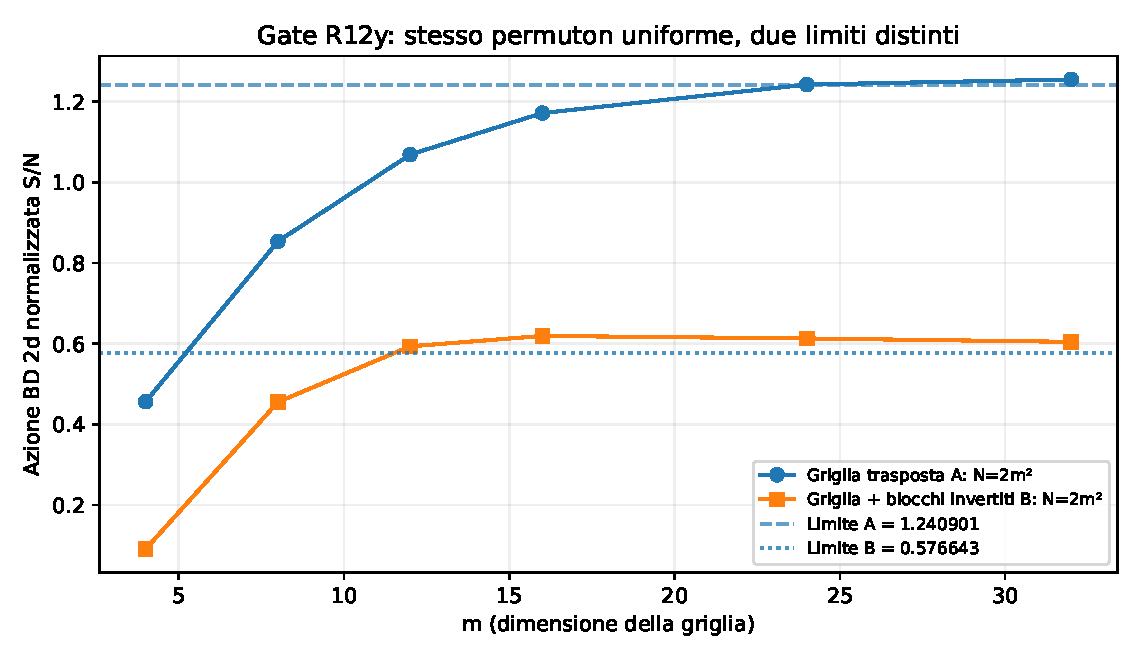
\includegraphics[width=0.85\textwidth]{r12y_uniform_permuton_no_go.pdf}
\caption{R12y. Due successioni di permutazioni con lo stesso permuton uniforme e stessa taglia per ogni $m$, ma azioni normalizzate che tendono a valori distinti. I valori limite sono derivati dalla serie dei divisori, non ottenuti estrapolando il grafico.}
\end{figure}

\begin{figure}[H]
\centering
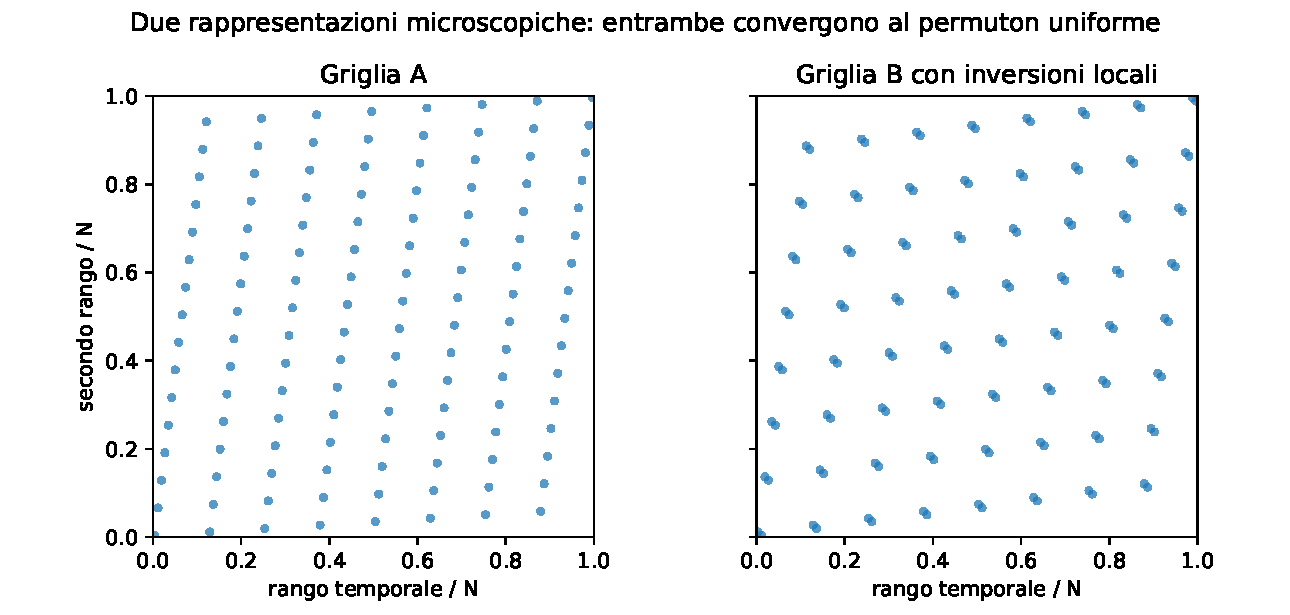
\includegraphics[width=0.82\textwidth]{r12y_two_grid_examples.pdf}
\caption{R12y, $m=8$. Due microstrutture differenti rappresentate alla stessa taglia $N=128$. Il limite macroscopico di entrambe e il permuton uniforme; i dettagli degli intervalli di piccola cardinalita non sono visibili dalla sola convergenza debole.}
\end{figure}

\subsection{Controlli indipendenti, dominio del no-go e prossimo oggetto}

Le identita finite dei conteggi sono state confrontate su tutte le taglie prefissate con l'implementazione storica dell'azione \texttt{r12o\_mc.py}, senza cambiare $\epsilon$ o la normalizzazione. Tutti i $12$ controlli diagonali e i $6$ confronti A/B passano con errore assoluto $<10^{-7}$; i casi $N\le128$ passano inoltre la enumerazione tripla diretta degli intervalli. I dati e il programma sono nel pacchetto come \texttt{R12Y\_RESULTS.json}, \texttt{r12y\_permuton\_obstruction.py} e \texttt{R12Y\_ANALYSIS\_PLAN.json}.

\textbf{Cosa non segue dal risultato.} Non si e mostrato che $S_N/N$ non converga in probabilita sotto la permutazione uniforme, ne che sia impossibile una LDP congiunta o una descrizione complessa esatta. Due successioni deterministiche avvicinano lo stesso permuton ma possono avere probabilita infinitesime molto diverse. Il problema del sign del path sum a $g=1$ non e stato risolto. Il risultato non autorizza nessuna inferenza al path sum 4d non etichettato o a una cosmologia nuova.

Il dato mancante e precisamente la \emph{microstruttura degli intervalli}. Introducendo il profilo normalizzato $\nu_{N,k}=N_k/N$, Eq.~\eqref{eq:r12y_action} diventa l'identita
\begin{equation}
 \frac{S_\epsilon}{N}=4\epsilon\left[1-2\epsilon\sum_{k\ge0}f_\epsilon(k)\nu_{N,k}\right].\label{eq:r12y_microprofile}
\end{equation}
Il vettore $\nu_N$ distingue le due famiglie: e dunque un candidato naturale per uno \emph{stato arricchito} $(\gamma,\nu)$, non una nuova legge fisica gia derivata. Una convergenza sufficientemente forte del profilo, per esempio con controllo delle code nel peso $(1-\epsilon)^k(1+k^2)$, renderebbe continuo questo osservabile. Resta \emph{da dimostrare} se i profili siano tight alle scale rilevanti e se esista una LDP congiunta controllabile: la sola LDP dei permutons non fornisce tale informazione. Inoltre un principio di Laplace per pesi reali positivi non giustifica automaticamente saddle complessi per $e^{igS}$.

\subsection{Verdetto del Gate R12y}

\textbf{Gate R12y:}
\begin{quote}
\status{A GLOBAL PERMUTON-ONLY CONTINUOUS ACTION FUNCTIONAL FOR THE R12N--R12X NORMALIZED 2D BD ACTION IS RULED OUT BY EXPLICIT SEQUENCES. THE OBSTRUCTION HOLDS EVEN AT THE UNIFORM PERMUTON, WITH TWO DISTINCT ANALYTIC LIMITS AT FIXED $\epsilon=0.21$. EXACT INTERVAL-COUNT IDENTITIES AND INDEPENDENT HISTORICAL-CODE CHECKS PASS. TYPICAL-ENSEMBLE CONVERGENCE, JOINT LARGE DEVIATIONS AND LORENTZIAN SADDLES REMAIN UNRESOLVED. FINAL CLASSIFICATION:} \nolinkurl{R12Y_PERMUTON_ONLY_NORMALIZED_ACTION_NO_GO_EVEN_AT_LEBESGUE_PERMUTON}.
\end{quote}

Il prossimo Gate R12z deve quindi testare se la coppia permuton/profilo d'intervalli ammetta una legge limite sufficientemente forte, e se la microstruttura che sopravvive sia compatibile con una LDP \emph{del benchmark 2d}. Il Gate R13 resta \textbf{BLOCCATO}.



\section{Gate R12z: profilo d'intervalli, deriva logaritmica e cancellazione esatta}
\label{sec:r12z}

R12y ha escluso una rappresentazione \emph{globale} dell'azione normalizzata mediante il solo permuton debole. R12z prende come oggetto il profilo $\nu_{N,k}=N_k/N$ introdotto in Eq.~\eqref{eq:r12y_microprofile} e verifica, prima di invocare una LDP congiunta, che tipo di limite possieda sotto la \emph{misura uniforme positiva} sulle permutazioni. Il parametro dell'azione rimane $\epsilon=0.21$ e non viene effettuato alcun fit.

\subsection{Protocollo preregistrato e dominio del risultato}

Il piano \texttt{R12Z\_ANALYSIS\_PLAN.json} e stato scritto e sottoposto a SHA-256 prima dell'analisi. I risultati primari sono identita per qualunque $0<\epsilon<1$; i controlli numerici fissano il valore storico $\epsilon=0.21$. Il benchmark resta l'ensemble \emph{representation-weighted} degli ordini 2d associati a permutazioni uniformi, non il path sum Lorentziano non etichettato in quattro dimensioni. Sono stati congelati i test esatti $N=2,\ldots,7$, le cinque taglie prospettiche $N=16,32,64,128,256$, tre repliche da $2048$ permutazioni indipendenti e i cutoff inclusivi $K=8,16,24,40,64$.

\subsection{Teorema: media esatta dell'intero profilo}

Sia $N_k$ il numero di coppie comparabili il cui intervallo aperto contiene esattamente $k$ elementi. Scriviamo $H_j=\sum_{s=1}^j s^{-1}$, con $H_0=0$. Vale per ogni $N\ge2$, $0\le k\le N-2$:
\begin{equation}
\boxed{\frac{\mathbb E[N_k]}{N}=H_{N-1}-H_k-2+\frac{k+1}{N}\left(H_N-H_{k+1}+2\right).}\label{eq:r12z_mean_nk}
\end{equation}
La dimostrazione usa $N$ punti indipendenti uniformi nel quadrato, equivalenti dopo ordinamento in ascissa a una permutazione uniforme. Una coppia orientata causalmente ha separazioni coordinate $u,v\in(0,1)$ e, condizionate tali separazioni, le altre $N-2$ particelle contribuiscono all'intervallo secondo $K\sim\mathrm{Bin}(N-2,uv)$. Quindi
\begin{align}
\mathbb E[N_k]=N(N-1)\binom{N-2}{k}\int_0^1\!\int_0^1
 &(1-u)(1-v)(uv)^k\\
 &\times(1-uv)^{N-2-k}\,du\,dv.\label{eq:r12z_pair_integral}
\end{align}
Ponendo $z=uv$, il kernel di prodotto e $W(z)=-(1+z)\ln z-2(1-z)$. L'integrale binomiale normalizzato induce una variabile $Z\sim\mathrm{Beta}(k+1,N-1-k)$ e si riduce a $\mathbb E[N_k]/N=\mathbb E[W(Z)]$. Le identita beta per $\mathbb E[\ln Z]$ e $\mathbb E[Z\ln Z]$ danno direttamente Eq.~\eqref{eq:r12z_mean_nk}; non intervengono assunzioni asintotiche.

In particolare,
\begin{equation}
\frac{\mathbb E[N_0]}{N}=\left(1+\frac1N\right)H_N-2,\qquad
\frac{\mathbb E[N_k]}{N}=\ln N+\gamma_E-H_k-2+o(1)\quad(k\ \text{fissato}).\label{eq:r12z_log_mean}
\end{equation}
\emph{Precisazione logica:} questo dimostra la divergenza delle \emph{medie} di ciascuna coordinata grezza $\nu_{N,k}$ a $k$ fissato, e l'assenza di un bound uniforme in aspettazione per la norma positiva pesata che include $k=0$. \textbf{Non} dimostra, da solo, divergenza in probabilita della coordinata, ne esclude una LDP per un oggetto opportunamente rinormalizzato. La scelta iniziale del profilo grezzo come vettore a coordinate con limite finito richiede dunque una correzione.

\begin{figure}[H]
\centering
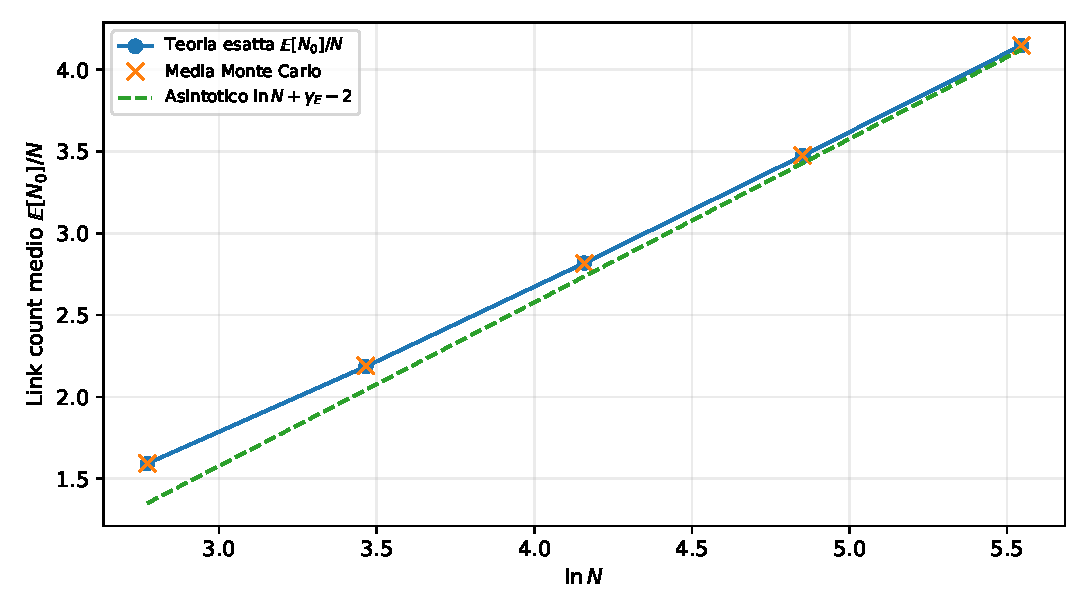
\includegraphics[width=0.79\textwidth]{r12z_log_profile.pdf}
\caption{R12z. Crescita logaritmica esatta della media dei link $N_0/N$ e confronto con le nuove simulazioni uniformi. Non e una stima di scaling fisico Lorentziano.}
\end{figure}

\subsection{Teorema: cancellazione esatta della deriva nell'azione}

Con $q=1-\epsilon$ e con $f_\epsilon(k)$ \emph{identico} a R12y, la funzione generatrice soddisfa
\begin{equation}
F_\epsilon(z)=\sum_{k\ge0}f_\epsilon(k)z^k=\frac{(1-z)^2}{(1-qz)^3},\qquad F_\epsilon(1)=F_\epsilon'(1)=0.\label{eq:r12z_double_zero}
\end{equation}
Quindi $\sum_k f_\epsilon(k)=\sum_k kf_\epsilon(k)=0$: e la somma \emph{firmata}, non la norma positiva dei conteggi, a cancellare le parti divergenti. Per $K\sim\mathrm{Bin}(N-2,z)$ si verifica inoltre l'identita
\begin{equation}
\mathbb E[f_\epsilon(K)\mid z]=\frac12\frac{d^2}{dz^2}\big[z^2(1-\epsilon z)^{N-2}\big].\label{eq:r12z_f_binomial}
\end{equation}
Sostituendola in Eq.~\eqref{eq:r12z_pair_integral} dopo la somma su $k$ e integrando per parti due volte in $u$, l'integrale doppio diventa unidimensionale:
\begin{align}
\mathbb E\left[\sum_{k=0}^{N-2}N_kf_\epsilon(k)\right]
&=\frac{N(N-1)}2\int_0^1(1-v)(1-\epsilon v)^{N-2}\,dv\\
&=\frac{N\epsilon-1+(1-\epsilon)^N}{2\epsilon^2}.\label{eq:r12z_weighted_identity}
\end{align}
Ne deriva \emph{esattamente per ogni $N\ge2$}:
\begin{equation}
\boxed{\mathbb E[S_N]=4\left[1-(1-\epsilon)^N\right]\ \longrightarrow\ 4.}\label{eq:r12z_exact_ES}
\end{equation}
L'origine della centratura $S_N-4$ usata empiricamente in R12w riceve cosi una giustificazione esatta \emph{per la media dell'ensemble uniforme}, senza che cio imponga una varianza limite, una fase non oscillante o una misura Lorentziana convergente. Il risultato e ottenuto qui per il benchmark e non viene presentato come novita assoluta nella letteratura BD.

\begin{figure}[H]
\centering
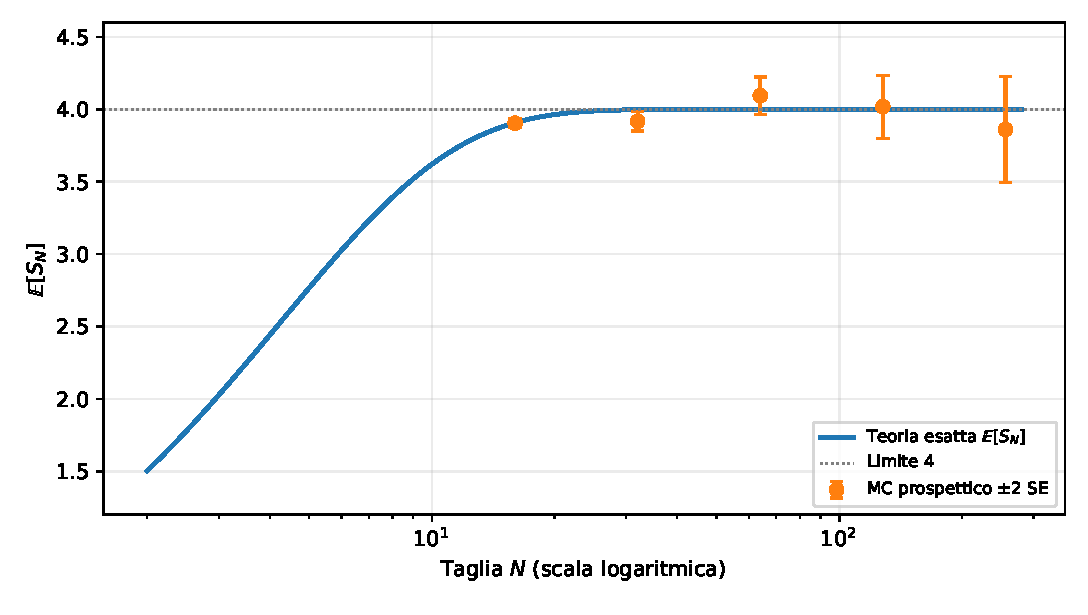
\includegraphics[width=0.77\textwidth]{r12z_exact_mean_action.pdf}
\caption{R12z. Formula chiusa $\mathbb E[S_N]=4[1-(1-\epsilon)^N]$, nuova validazione Monte Carlo e limite $4$. Le barre riportano $\pm2$ errori standard dei campioni indipendenti.}
\end{figure}

\subsection{Profilo centrato, replay prospettico e code pesate}

Una nuova variabile a media esattamente nulla e
\begin{equation}
\delta\nu_{N,k}=\frac{N_k-\mathbb E[N_k]}{N},\quad
Y_N=\frac{S_N-\mathbb E[S_N]}{N}=-8\epsilon^2\sum_{k=0}^{N-2}f_\epsilon(k)\,\delta\nu_{N,k}.\label{eq:r12z_compensated_profile}
\end{equation}
La seconda uguaglianza e una \emph{identita a taglia finita}, non una postulata rinormalizzazione dinamica. Per un cutoff $K$ prefissato, $Y_{N,K}$ si ottiene troncando la somma a $k\le K$. L'errore relativo riportato sotto e il rapporto tra RMS del residuo $Y_N-Y_{N,K}$ e RMS dell'osservabile completo; i cutoff erano fissati nel piano precedente ai dati.

\begin{table}[H]
\centering
\small
\begin{tabular}{rrrrr}
\toprule
$N$ & $\mathbb E[\nu_0]$/MC & $\mathbb E[S]$/MC & residuo $K=24$ & residuo $K=40$\\
\midrule
16 & 1.592/1.594 & 3.908/3.905 & 0.00\% & 0.00\%  \\
32 & 2.185/2.190 & 3.998/3.918 & 0.13\% & 0.00\%  \\
64 & 2.818/2.815 & 4.000/4.095 & 1.71\% & 0.04\%  \\
128 & 3.476/3.476 & 4.000/4.018 & 3.49\% & 0.18\%  \\
256 & 4.148/4.149 & 4.000/3.860 & 3.79\% & 0.26\%  \\
\bottomrule
\end{tabular}
\caption{R12z. Teoria esatta contro medie di tre repliche da 2048 permutazioni; le colonne finali sono percentuali del residuo RMS della somma \emph{centrata}. Nessun cutoff e stato scelto dopo i risultati.}
\end{table}

L'enumerazione completa di $2!,\ldots,7!$ permutazioni riproduce ogni media $\mathbb E[N_k]/N$ e $\mathbb E[S_N]$ entro $7\times10^{-15}$; il replay confronta istogrammi indipendenti, valutatore storico e calcolo matriciale. Le cinque medie pooled, ciascuna su tre repliche indipendenti, superano il controllo a cinque errori standard rispetto alla media teorica dell'azione. L'accordo non prova pero una legge limite. In particolare, il rapporto di varianza empirico $\mathrm{Var}(Y_N)$ cambia sensibilmente fra $N=64$ e $N=256$, per cui non si estrapola lo scaling $N^2$ osservato nella finestra piu corta R12w.

\begin{figure}[H]
\centering
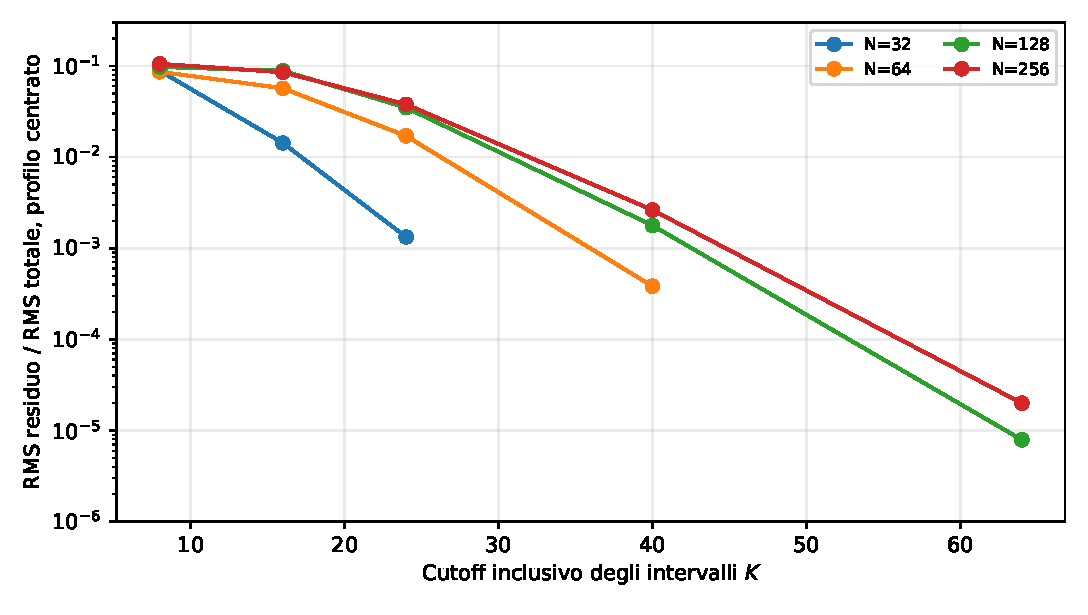
\includegraphics[width=0.78\textwidth]{r12z_compensated_tails.pdf}
\caption{R12z. Residuo relativo RMS dopo compensazione esatta di ogni $N_k$. Il decadimento ai cutoff prefissati e un risultato di \emph{taglia finita}; non e un teorema di tightness uniforme o una LDP congiunta.}
\end{figure}

\subsection{Verdetto R12z e oggetto del prossimo gate}

R12z corregge il candidato di R12y: il profilo non centrato $\nu_{N,k}$ possiede medie logaritmicamente divergenti sotto la misura uniforme in media, mentre l'azione usa una somma firmata con cancellazioni esatte. Il profilo \emph{centrato} e una rappresentazione algebrica esatta delle fluttuazioni, non ancora uno stato limite dimostrato; le code sono numericamente piccole nella finestra esplorata ma manca un bound uniforme in $N$. La LDP del permuton non puo essere trasferita automaticamente alla coppia arricchita, e una LDP positiva non determina il path sum a fase complessa $e^{igS}$.

\textbf{Gate R12z:}\par
\nolinkurl{R12Z_EXACT_MEAN_CANCELLATION_PASS_RAW_PROFILE_DIVERGENT_MEANS_JOINT_LDP_OPEN}.

R12aa dovra fissare una norma di coda e tentare una prova o un controesempio per la tightness della famiglia compensata, quindi affrontare separatamente una possibile LDP congiunta. Il path sum 4d e il Gate R13 restano \textbf{BLOCCATI}.


\section{Gate R12aa: curvatura discreta e cutoff logaritmico controllato}
\label{sec:r12aa}

R12z ha costruito una cancellazione esatta nella media dell'azione, ma non aveva dimostrato un limite dell'intero profilo di intervalli. R12aa separa tre questioni differenti: (i) esiste una rappresentazione discreta in cui la deriva logaritmica e eliminata algebricamente? (ii) le code possono essere controllate \emph{uniformemente} senza scegliere un cutoff dopo aver visto i dati? (iii) quali inferenze probabilistiche non seguono da questi risultati? Il benchmark rimane quello delle permutazioni uniformi di ordini 2d \emph{representation-weighted}; il valore storico dell'accoppiamento e $\epsilon=0.21$, senza modifiche.

\subsection{Protocollo congelato e riproducibilita}

Il piano \texttt{R12AA\_ANALYSIS\_PLAN.json} e stato congelato prima dei nuovi campionamenti, includendo definizioni, test analitici, costruzioni avverse e finestre numeriche. Sono previste enumerazioni esaustive $N=2,\ldots,8$, verifiche indipendenti contro l'azione di R12o, e nuovi holdout a $N=64,128,256,512,1024$ con tre repliche indipendenti per taglia. Le dimensioni campionarie per replica sono rispettivamente $512,512,512,256,128$. I cutoff diagnostici fissi sono $K=8,16,24,40,64$; quello teorico usa $\delta=1/2$. Gli script, le repliche e il checksum del piano sono conservati nel pacchetto incrementale della presente versione.

\subsection{Teorema deterministico: l'azione e una seconda differenza}

Con $q=1-\epsilon\in(0,1)$, e con $N_k=0$ per $k\ge N-1$, riprendiamo i coefficienti dell'azione di Eq.~\eqref{eq:r12y_f}. La loro funzione generatrice ha una fattorizzazione esatta:
\begin{equation}
F(z)=\sum_{k\ge0}f_\epsilon(k)z^k
=\frac{(1-z)^2}{(1-qz)^3}.
\label{eq:r12aa_generating}
\end{equation}
Definendo $g_k=\binom{k+2}{2}q^k$ per $k\ge0$ e $g_{-1}=g_{-2}=0$, segue per confronto dei coefficienti
\begin{equation}
f_\epsilon(k)=g_k-2g_{k-1}+g_{k-2}.
\label{eq:r12aa_second_diff_weight}
\end{equation}
Lo spostamento finito degli indici dimostra, \emph{per ciascuna permutazione},
\begin{equation}
\boxed{\sum_{k\ge0}f_\epsilon(k)N_k
=\sum_{k\ge0}g_k\bigl(N_k-2N_{k+1}+N_{k+2}\bigr).}
\label{eq:r12aa_discrete_curvature}
\end{equation}
La somma resta finita sul lato destro poiche $N_k=0$ oltre la cardinalita massima. La nuova variabile naturale e la \emph{curvatura discreta del profilo}
\begin{equation}
\mathcal C_N(k)=\frac{N_k-2N_{k+1}+N_{k+2}}{N}.
\label{eq:r12aa_curvature}
\end{equation}
Questo e un cambiamento di rappresentazione \emph{esatto}, non un limite stocastico. La positivit\`a dei pesi $g_k$ non implica la positivit\`a delle curvatura $\mathcal C_N(k)$ per singola realizzazione.

\subsection{Media esatta della curvatura}

Applicando due differenze alla Eq.~\eqref{eq:r12z_mean_nk}, con $\mathbb E[N_{N-1}]=\mathbb E[N_N]=0$, si ottiene per $0\le k\le N-2$:
\begin{equation}
\boxed{\mathbb E[\mathcal C_N(k)]
=\frac{N-k-1}{N(k+1)(k+2)}
\longrightarrow\frac{1}{(k+1)(k+2)}\quad(N\to\infty,\ k\ \mathrm{fisso}).}
\label{eq:r12aa_curvature_mean}
\end{equation}
Cosi la deriva $\ln N$ delle medie grezze scompare esattamente. Inoltre, poiche $g_k/[(k+1)(k+2)]=q^k/2$,
\begin{align}
\frac{1}{N}\mathbb E\!\left[\sum_{k\ge0}f_\epsilon(k)N_k\right]
&=\frac{1}{2N}\sum_{k=0}^{N-2}(N-k-1)q^k\\
&=\frac{N\epsilon-1+q^N}{2N\epsilon^2},
\label{eq:r12aa_action_check}
\end{align}
che ricostruisce senza ipotesi asintotiche $\mathbb E[S_N]=4(1-q^N)$. La convergenza delle \emph{medie} di $\mathcal C_N(k)$ non costituisce una dimostrazione della tightness, della concentrazione o della convergenza in legge.

\begin{figure}[H]
\centering
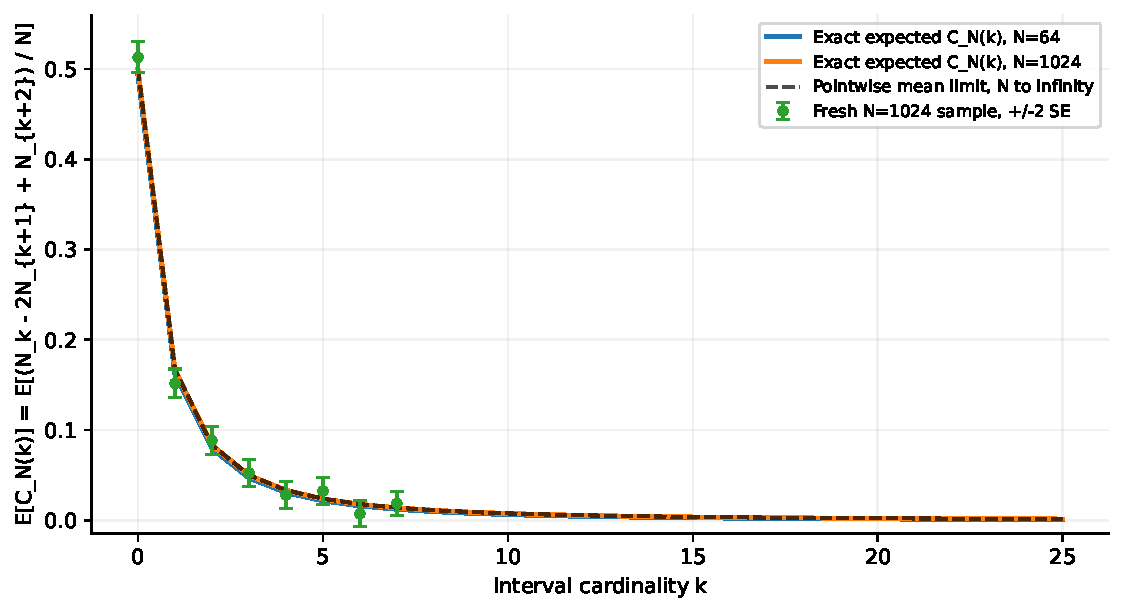
\includegraphics[width=0.91\textwidth]{r12aa_curvature_mean.pdf}
\caption{Curvatura discreta: formula di media esatta, limite a $k$ fissato e controllo numerico indipendente a $N=1024$. Le barre riportano soltanto $\pm2$ errori standard del campione positivo.}
\label{fig:r12aa_curvature}
\end{figure}

\subsection{Teorema uniforme: bastano $O(\log N)$ cardinalita}

Poniamo $Y_N=(S_N-\mathbb E[S_N])/N$ e la sua versione che usa soltanto le cardinalita $k\le K$:
\begin{equation}
Y_{N,K}=-8\epsilon^2\sum_{k=0}^{K} f_\epsilon(k)\frac{N_k-\mathbb E[N_k]}{N}.
\label{eq:r12aa_cutoff_def}
\end{equation}
Poiche per tutte le permutazioni $0\le N_k,\mathbb E[N_k]\le N(N-1)/2$, segue la stima \emph{deterministica}
\begin{equation}
|Y_N-Y_{N,K}|\le4\epsilon^2(N-1)\sum_{k>K}|f_\epsilon(k)|.
\label{eq:r12aa_prebound}
\end{equation}
Per $m=K+1$, stimando separatamente i tre monomi del polinomio in $k$ e sommando le serie geometriche, si ha
\begin{equation}
\sum_{k\ge m}|f_\epsilon(k)|\le q^m
\left[\frac{4}{\epsilon}+\frac{3m}{q}
+\frac{\epsilon m(m-1)}{2q^2}\right]\equiv B_m.
\label{eq:r12aa_weight_tail}
\end{equation}
Dunque
\begin{equation}
\boxed{\sup_{\pi\in\mathfrak S_N}|Y_N(\pi)-Y_{N,K}(\pi)|
\le4\epsilon^2(N-1)B_{K+1}.}
\label{eq:r12aa_uniform_tail}
\end{equation}
Per ogni $\delta>0$ scegliere, \emph{prima di osservare i dati},
\begin{equation}
K_N=\left\lceil\frac{(1+\delta)\ln N}{-\ln q}\right\rceil.
\label{eq:r12aa_log_cutoff}
\end{equation}
Essendo $q^{K_N}\le N^{-(1+\delta)}$, il lato destro della Eq.~\eqref{eq:r12aa_uniform_tail} e $O(N^{-\delta}(\ln N)^2)\to0$ per ogni permutazione. Il cutoff si estende quindi solo come $\log N$, e il suo errore \emph{normalizzato} e controllato uniformemente. Lo stesso limite vale per $S_N/N$ senza centrare, rispetto al corrispondente troncamento delle somme; la parte costante $4\epsilon$ non cambia. Questo risultato riguarda una approssimazione \emph{triangolare a dimensione crescente}, non un funzionale continuo su un profilo a dimensione fissa, ne una LDP.

\subsection{No-go per il controllo deterministico a cutoff fisso}

Fissiamo $K$ e scegliamo un intero $k>K$ per cui $f_\epsilon(k)\ne0$ (ce ne sono sempre, essendo il fattore polinomiale di grado due). Consideriamo $N=2m+k$ elementi disposti in tre blocchi consecutivi: un'antichain di $m$ valori bassi decrescenti, una catena centrale crescente di $k$ valori, e un'antichain di $m$ valori alti decrescenti. Ciascuna delle $m^2$ coppie fra primo e terzo blocco ha esattamente $k$ elementi nel suo intervallo aperto; le altre coppie comparabili sono $O(mk+k^2)$. Per $K=k-1$ in particolare non vi sono altri contributi con cardinalita $>K$. Si ha quindi
\begin{equation}
\frac{S_N-S_{N,K}}{N}
=-8\epsilon^2\,f_\epsilon(k)\,\frac{m^2}{2m+k}+O(1),
\label{eq:r12aa_fixed_K_obstruction}
\end{equation}
con divergenza lineare per $m\to\infty$. La stessa conclusione vale per l'errore \emph{centrato}, dato che la correzione delle medie e al piu $O(\ln N)$ a $K$ fissato. Quindi \textbf{nessun cutoff $K$ fissato fornisce un errore che si annulli uniformemente su tutte le permutazioni}. Le due famiglie preregistrate $k=9$ e $k=25$ riproducono la costruzione senza altri conteggi oltre $k$.

Questo no-go deterministico non esclude che le permutazioni patologiche diventino rare sotto la misura uniforme; non equivale a un risultato negativo di \emph{tightness in probabilita}.

\subsection{Validazioni finite e limite della lettura di R12w}

Enumerando tutte le permutazioni per $N=2,\ldots,8$ si verificano il conteggio, la formula esatta della media, il replay storico e il secondo differenziale, senza anomalie. Gli holdout nuovi usano complessivamente $1536,1536,1536,768,384$ permutazioni indipendenti alle cinque taglie. La Tab.~\ref{tab:r12aa_holdout} riporta grandezze \emph{descrittive}, non stime confermative di un esponente.

\begin{table}[H]
\centering\small
\begin{tabular}{rrrrrr}
\toprule
$N$ & $K_N$ & $\widehat{\mathrm{sd}}(S_N/N)$ & RMS coda $K=24$ & RMS coda $K_N$ & bound uniforme $K_N$\\
\midrule
64   & 27 & 0.07644 & 0.001375 & 0.000746 & 3.817 \\
128  & 31 & 0.06771 & 0.002354 & 0.000711 & 3.649 \\
256  & 36 & 0.05461 & 0.002157 & 0.000309 & 2.813 \\
512  & 40 & 0.04439 & 0.001541 & 0.000115 & 2.579 \\
1024 & 45 & 0.03493 & 0.001046 & 0.0000347 & 1.911 \\
\bottomrule
\end{tabular}
\caption{Nuovi campioni positivi indipendenti di R12aa, $\epsilon=0.21$, $\delta=1/2$. Le RMS sono medie delle tre repliche. Il bound e valido per \emph{ogni} permutazione, ma e molto piu largo degli errori osservati alle taglie finite: il fatto che vada a zero e una conclusione asintotica, non una certificazione di precisione millesimale alla taglia $1024$.}
\label{tab:r12aa_holdout}
\end{table}

\begin{figure}[H]
\centering
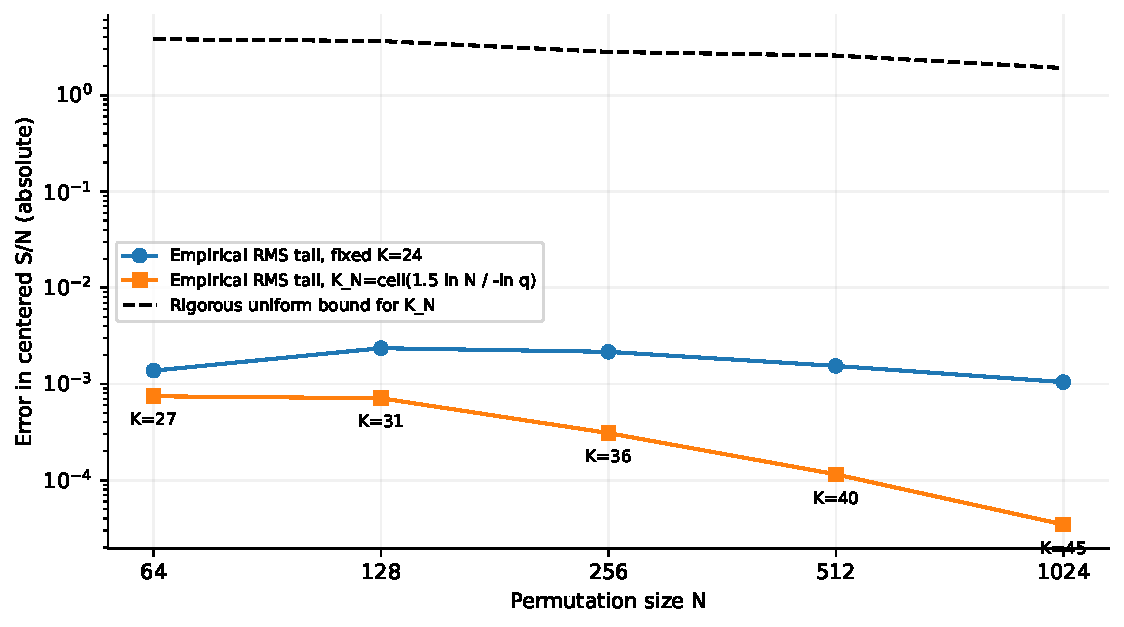
\includegraphics[width=0.9\textwidth]{r12aa_cutoff_control.pdf}
\caption{Code pesate misurate e confronto con la garanzia analitica. La forte differenza fra bound e RMS non e nascosta da un fit.}
\label{fig:r12aa_cutoff}
\end{figure}

\begin{figure}[H]
\centering
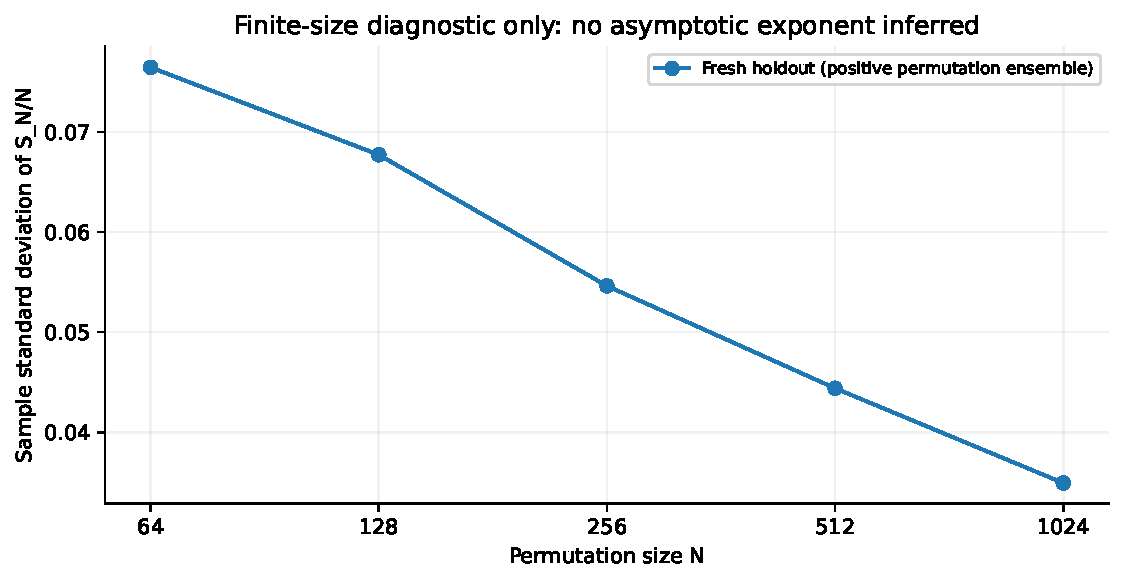
\includegraphics[width=0.85\textwidth]{r12aa_positive_dispersion.pdf}
\caption{Dispersione normalizzata sul nuovo holdout, riferita \emph{soltanto} alla misura positiva. Il fit $\mathrm{Var}(S)\propto N^{2.004}$ ottenuto da R12w su $N=24$--$64$ non deve essere interpretato come legge universale estendibile a queste taglie: qui non viene stimato nessun nuovo esponente asintotico.}
\label{fig:r12aa_dispersion}
\end{figure}

\subsection{Verdetto R12aa e stato della chiusura}

\begin{quote}
\small\noindent\status{EXACT CURVATURE / LOG CUTOFF: PASS;}\\\status{FIXED K: UNIFORM NO-GO; TYPICAL LIMIT: OPEN.}
\end{quote}

La seconda differenza del profilo e un oggetto algebricamente naturale; la sua media ha un limite esatto a cardinalita fissata. Una approssimazione dell'azione normalizzata per $K_N=O(\ln N)$ e ora \emph{provata} uniformemente; un cutoff fisso fallisce \emph{deterministicamente} nel dominio di tutte le permutazioni. Restano aperte la tightness e la legge limite dei profili \emph{casuali} a cardinalita fissa, la struttura di covarianza, una LDP congiunta e l'analisi delle fasi oscillanti. Il problema fisico originale e R13 non sono sbloccati.



\section{Gate R12ab: covarianze esatte e criterio per la concentrazione}
\label{sec:r12ab}

Il risultato di R12aa era deterministico: l'azione normalizzata puo essere ricostruita con un cutoff di intervalli crescente come $O(\ln N)$, ma le fluttuazioni di ciascuna coordinata non erano ancora controllate. In R12ab manteniamo $\epsilon=0.21$ e la misura uniforme sulle rappresentazioni per permutazione degli ordini 2d. Una \emph{covarianza della misura positiva} non viene identificata con il cumulante della misura oscillante $e^{iS}$, ne trasferita automaticamente agli insiemi causali Lorentziani non etichettati in 4d.

\subsection{Protocollo congelato e variabili elementari}

Il piano \texttt{R12AB\_PREREGISTRATION.json} viene fissato prima della nuova produzione numerica. Per $i<j$ e $k\ge0$ definiamo l'indicatore di intervallo aperto
\begin{equation}
A_{ij,k}(\pi)=\mathbf1_{\{\pi_i<\pi_j\}}
\mathbf1_{\{\#\{t:i<t<j,\;\pi_i<\pi_t<\pi_j\}=k\}},
\qquad N_k=\sum_{i<j}A_{ij,k}.
\label{eq:r12ab_indicator}
\end{equation}
L'orientazione $\pi_i<\pi_j$ fa parte della definizione; gli intervalli con estremi incomparabili non sono contati. Se $L=j-i+1$, la probabilita marginale e una identita combinatoria:
\begin{equation}
\boxed{p_{ij}(k):=\mathbb P(A_{ij,k}=1)=\frac{L-k-1}{L(L-1)}}
\quad(0\le k\le L-2),
\label{eq:r12ab_marginal}
\end{equation}
con probabilita nulla fuori dall'intervallo indicato. Infatti i due estremi hanno due ranghi ordinati che differiscono di $k+1$ in esattamente $L-k-1$ casi sui $L(L-1)$ ordinamenti possibili dei ranghi estremi.

\subsection{Probabilita congiunta: il contributo delle finestre sovrapposte}

Siano $I=(i,j)$ e $J=(u,v)$. Se i segmenti \emph{posizionali completi} $[i,j]$ e $[u,v]$ sono disgiunti, gli ordinamenti relativi dei valori che occupano i due segmenti sono indipendenti sotto la permutazione uniforme. Ne segue
\begin{equation}
\mathbb E[A_{I,k}A_{J,l}]=p_I(k)p_J(l)
\qquad\text{se } j<u\text{ oppure }v<i.
\label{eq:r12ab_disjoint}
\end{equation}
Negli altri casi occorre conservare la dipendenza. Una formula integrale esatta si ottiene rappresentando la permutazione come ranghi di variabili $X_t$ indipendenti uniformi su $(0,1)$. Sia $E$ l'insieme degli indici distinti fra $i,j,u,v$; dati i valori $x_e$, indichiamo con $U=(x_i,x_j)$ e $V=(x_u,x_v)$ gli intervalli di valori, quando gli estremi sono orientati crescentemente. Gli estremi dell'altra coppia interni al primo segmento contribuiscono \emph{deterministicamente} a due conteggi $b_I,b_J$. Per ogni indice non appartenente a $E$, il fattore generatore $P_t(z,w;\mathbf x)$ e
\begin{equation}
P_t=\begin{cases}
1-|U|+|U|z,&t\in(i,j)\setminus(u,v),\\
1-|V|+|V|w,&t\in(u,v)\setminus(i,j),\\
1-|U\cup V|+|U\setminus V|z+|V\setminus U|w+|U\cap V|zw,
&t\in(i,j)\cap(u,v),\\
1,&\text{altrimenti}.
\end{cases}
\label{eq:r12ab_generating_factors}
\end{equation}
Qui le barre indicano la lunghezza dell'intervallo \emph{di valori}, non il numero di elementi. Pertanto, ponendo $O(\mathbf x)=\mathbf1_{x_i<x_j}\mathbf1_{x_u<x_v}$,
\begin{equation}
\boxed{\mathbb P(A_{I,k}=1,A_{J,l}=1)=
\int_{[0,1]^{|E|}}[z^kw^l]\left\{O(\mathbf x)
 z^{b_I(\mathbf x)}w^{b_J(\mathbf x)}
\prod_{t\notin E}P_t(z,w;\mathbf x)\right\}\,d\mathbf x.}
\label{eq:r12ab_exact_joint}
\end{equation}
La formula comprende il caso di un estremo condiviso e quello in cui un estremo dell'altra coppia cade nell'interno della prima; non moltiplica probabilita marginali in presenza di sovrapposizioni. Poiche l'evento dipende soltanto dall'ordinamento relativo delle posizioni nell'unione delle due finestre, per unione di $m$ posizioni la stessa probabilita si calcola in forma \emph{esatta razionale} enumerando i $m!$ ordinamenti di rango.

Definiamo $\Gamma_N(k,l)=\mathrm{Cov}(N_k,N_l)$. Espandendo la somma degli indicatori ed eliminando soltanto i termini indipendenti \emph{dimostrati}, si ha
\begin{align}
\Gamma_N(k,l)&=\sum_{I,J:\,[I]\cap[J]\ne\varnothing}
\bigl[\mathbb P(A_{I,k}=1,A_{J,l}=1)-p_I(k)p_J(l)\bigr],\\
\Sigma_N(k,l):=\mathrm{Cov}(\mathcal C_N(k),\mathcal C_N(l))
&=\frac1{N^2}\sum_{a,b=0}^2 d_a d_b\,\Gamma_N(k+a,l+b),\qquad (d_0,d_1,d_2)=(1,-2,1).
\label{eq:r12ab_covariance_formula}
\end{align}
Questa e una rappresentazione \emph{finita esatta}: non implica ancora che le sue componenti tendano a zero con $N$.

\subsection{Teorema-criterio: quale forma quadratica deve annullarsi?}

Per $g_k=\binom{k+2}{2}q^k$, $q=1-\epsilon$, riprendiamo da R12aa
\begin{equation}
Y_N=\frac{S_N-\mathbb E S_N}{N}
=-8\epsilon^2\sum_{k\ge0}g_k
[\mathcal C_N(k)-\mathbb E\mathcal C_N(k)].
\label{eq:r12ab_centered}
\end{equation}
Definiamo la somma troncata $Y^{\mathcal C}_{N,K}$ a $k\le K$ e la forma quadratica di covarianza
\begin{equation}
Q_{N,K}:=\sum_{k,l=0}^K g_kg_l\,\Sigma_N(k,l)\ge0,
\qquad \|Y^{\mathcal C}_{N,K}\|_2=8\epsilon^2\sqrt{Q_{N,K}}.
\label{eq:r12ab_qform}
\end{equation}
Poiche $0\le N_k\le N(N-1)/2$, si ha $|\mathcal C_N(k)-\mathbb E\mathcal C_N(k)|\le2(N-1)$. Per $m=K+1$ la coda dei pesi positivi ammette la somma \emph{esatta}
\begin{equation}
G_m:=\sum_{k=m}^{\infty}g_k=q^m\left[
\frac{(m+1)(m+2)}{2\epsilon}
+\frac{(2m+3)q}{2\epsilon^2}
+\frac{q(1+q)}{2\epsilon^3}\right].
\label{eq:r12ab_gtail}
\end{equation}
Con $a_{N,K}=16\epsilon^2(N-1)G_{K+1}$ segue la stima deterministica uniforme e il criterio in $L^2$:
\begin{equation}
\boxed{\sup_{\pi\in\mathfrak S_N}|Y_N-Y^{\mathcal C}_{N,K}|\le a_{N,K},
\qquad\left|\|Y_N\|_2-8\epsilon^2\sqrt{Q_{N,K}}\right|\le a_{N,K}.}
\label{eq:r12ab_l2_equiv}
\end{equation}
Per ogni $\delta>0$ e $K_N=\lceil(1+\delta)\ln N/(-\ln q)\rceil$, $a_{N,K_N}=O(N^{-\delta}(\ln N)^2)\to0$. Percio
\begin{equation}
\boxed{Y_N\to0\text{ in }L^2\quad\Longleftrightarrow\quad Q_{N,K_N}\to0.}
\label{eq:r12ab_concentration_criterion}
\end{equation}
Il teorema riduce quindi una eventuale \emph{prova} di concentrazione alla stima asintotica di una forma quadratica, e fornisce per $t>0$
\begin{equation}
\mathbb P(|Y_N|>t)\le
\frac{\left[8\epsilon^2\sqrt{Q_{N,K_N}}+a_{N,K_N}\right]^2}{t^2}.
\label{eq:r12ab_chebyshev}
\end{equation}
\textbf{Non e stato dimostrato che $Q_{N,K_N}\to0$.} La condizione e necessaria e sufficiente soltanto per la convergenza in $L^2$ dell'azione normalizzata; non dimostra da sola tightness dell'intero profilo, una CLT o una LDP congiunta. Il bound uniforme sulle code e matematicamente valido ma conservativo a $N$ finito.

\subsection{Enumerazione, test indipendenti e holdout}

Sono state enumerate integralmente le $N!$ permutazioni per $N=3,\ldots,8$, confrontando due implementazioni dell'istogramma e il valutatore storico R12o. Per $N\le6$ e stata inoltre ottenuta indipendentemente l'intera covarianza mediante la somma delle probabilita congiunte delle coppie, calcolate enumerando gli ordinamenti relativi delle posizioni nelle due finestre: differenza massima $<5\cdot10^{-16}$. Il test controlla anche semidefinitezza positiva e medie esatte del Gate R12aa.

L'holdout fresco usa tre repliche indipendenti ai valori preregistrati $N=64,128,256,512,1024$. Le taglie campionarie complessive sono, nell'ordine, $1536,1536,1152,768,384$. Le prime otto coordinate $k=0,\ldots,7$ sono fissate dal piano, senza selezione successiva. La Tab.~\ref{tab:r12ab_holdout} mostra le stime descrittive; le componenti fuori diagonale non vengono trascurate nel valutare la varianza di una somma pesata.

\begin{table}[H]
\centering\small
\begin{tabular}{rrrrr}
\toprule
$N$ & campioni & $\widehat{\mathrm{Var}}\,\mathcal C_N(0)$ & $\widehat{\mathrm{Cov}}(\mathcal C_0,\mathcal C_1)$ & $\widehat{\mathrm{sd}}(Y_N)$\\
\midrule
64&1536&0.176324&$-0.101251$&0.079643\\
128&1536&0.121648&$-0.068527$&0.066874\\
256&1152&0.074612&$-0.043468$&0.056572\\
512&768&0.046790&$-0.028732$&0.044777\\
1024&384&0.025284&$-0.015979$&0.036102\\
\bottomrule
\end{tabular}
\caption{R12ab: holdout positivo indipendente. Nessun esponente e fittato. La decrescita delle covarianze campionarie non dimostra da sola un rate teorico uniforme.}
\label{tab:r12ab_holdout}
\end{table}

\begin{figure}[H]
\centering
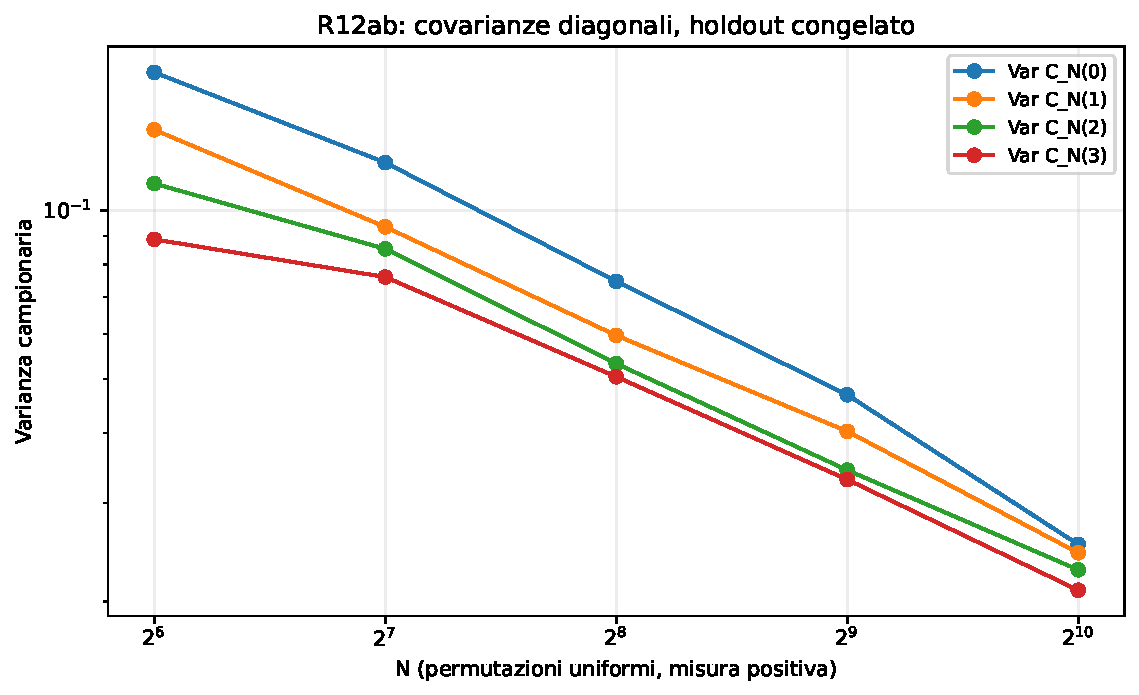
\includegraphics[width=0.85\textwidth]{r12ab_curvature_variance.pdf}
\caption{R12ab. Varianze empiriche delle prime quattro componenti della curvatura, su griglia preregistrata. L'asse $N$ non viene utilizzato per estrapolazioni confermative.}
\end{figure}
\begin{figure}[H]
\centering
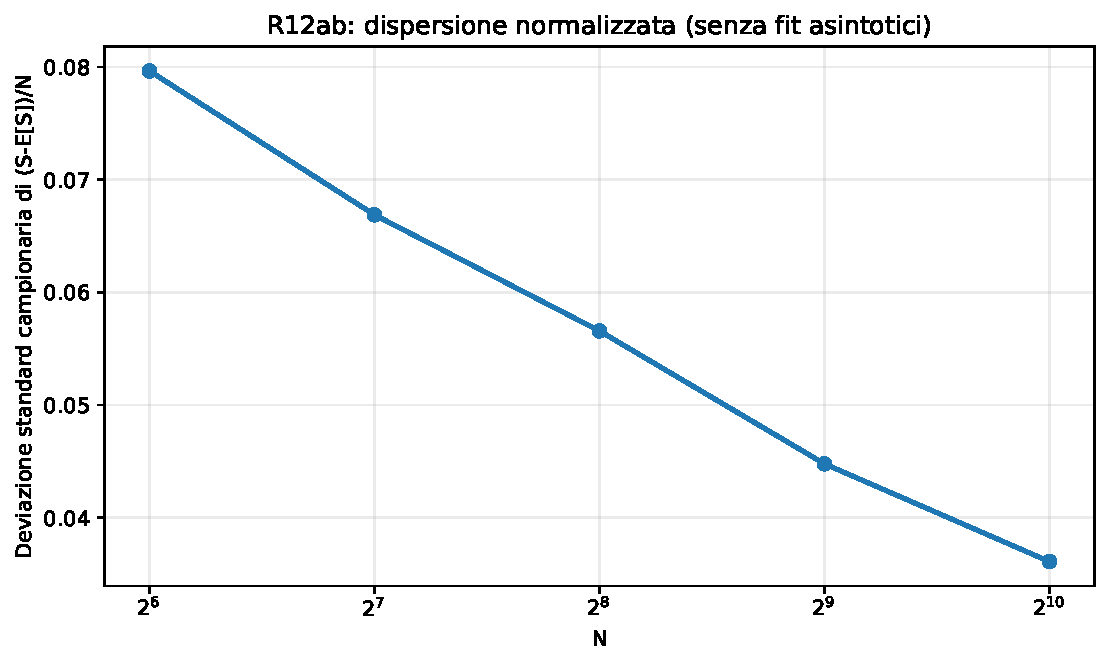
\includegraphics[width=0.82\textwidth]{r12ab_action_dispersion.pdf}
\caption{R12ab. Deviazione standard campionaria di $Y_N$ nella misura positiva; la diminuzione osservata non costituisce una dimostrazione di $L^2$-convergenza.}
\end{figure}
\begin{figure}[H]
\centering
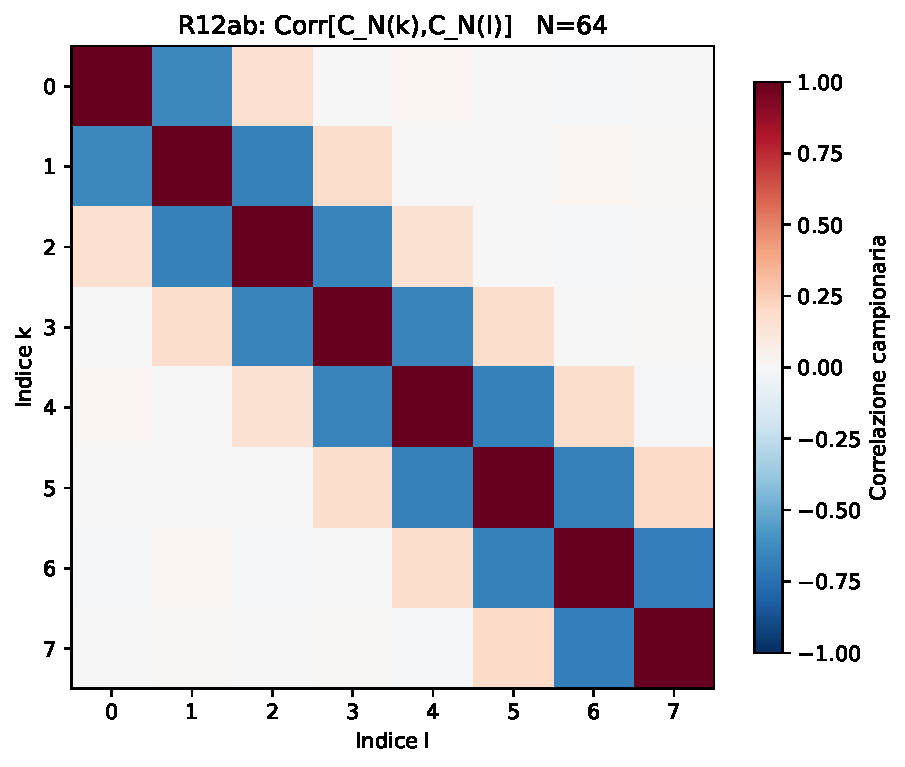
\includegraphics[width=0.69\textwidth]{r12ab_correlations_N64.pdf}
\caption{R12ab. Correlazioni fra le prime otto coordinate a $N=64$: contributi fuori diagonale non trascurabili.}
\end{figure}
\begin{figure}[H]
\centering
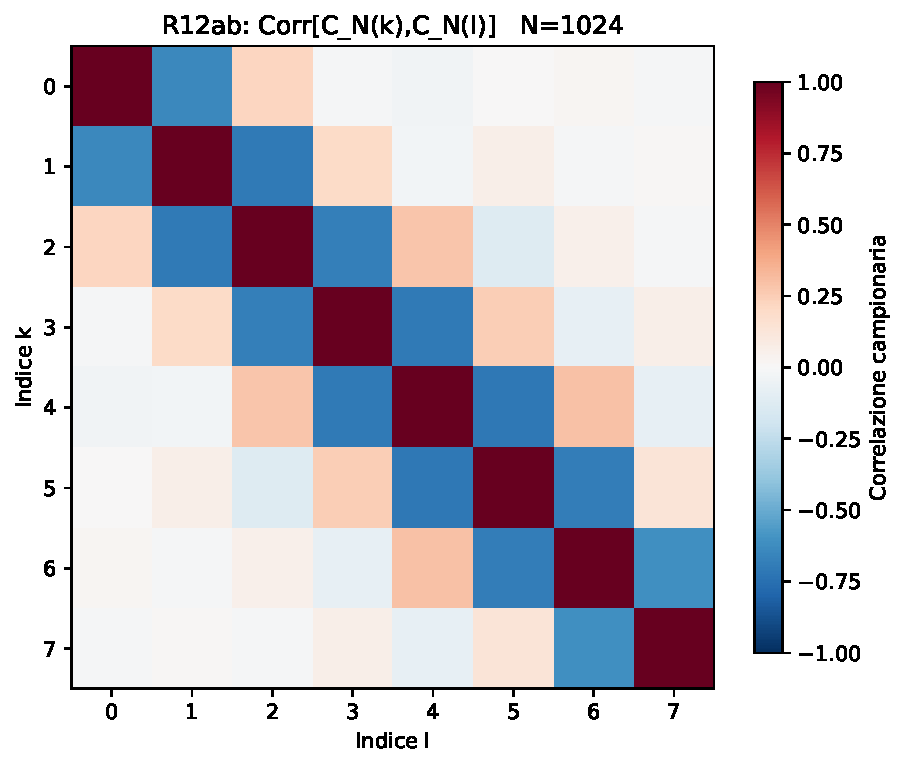
\includegraphics[width=0.69\textwidth]{r12ab_correlations_N1024.pdf}
\caption{R12ab. La stessa matrice a $N=1024$. Nessun limite di covarianza viene assunto a priori.}
\end{figure}

\subsection{Verdetto R12ab e problema successivo}

\begin{quote}
\small\noindent\status{EXACT FINITE-N COVARIANCE: PASS;}\\
\status{ASYMPTOTIC CONCENTRATION: OPEN.}
\end{quote}

\textbf{Gate R12ab:} \nolinkurl{R12AB_EXACT_COVARIANCE_REPRESENTATION_PASS_CONCENTRATION_OPEN}.
Le probabilita congiunte e la matrice di covarianza ammettono una rappresentazione esatta; l'enumerazione indipendente e gli holdout preregistrati superano i gate fissati. Il criterio $Q_{N,K_N}\to0$ e rigoroso \emph{come condizione}, ma non e verificato con un bound analitico asintotico. Il prossimo Gate R12ac tentera di controllare la forma quadratica di covarianza con stime teoriche di overlap/decoupling, registrando un eventuale no-go o un limite di risorse. I Gate R13 e la generalizzazione Lorentziana fisica restano \textbf{BLOCCATI}.


\section{Gate R12ac: Efron--Stein, rettangoli vuoti e concentrazione $L^2$}
\label{sec:r12ac}

Il Gate R12ab aveva ridotto la concentrazione dell'azione normalizzata all'annullamento di una forma quadratica delle covarianze. R12ac fornisce un bound positivo tramite un metodo diverso dal fit numerico: rappresentare la permutazione come l'ordine relativo di punti indipendenti in un quadrato. Il piano \texttt{R12AC\_PREREGISTRATION.json} e il suo SHA-256 sono stati congelati \emph{prima} delle nuove verifiche. Manteniamo $\epsilon=0.21$; le dimostrazioni valgono per ogni $0<\epsilon<1$ con costanti dipendenti da $\epsilon$.

\subsection{Enunciato: limite superiore della varianza positiva}

Per $q=1-\epsilon$, si considerino i pesi storici dell'azione BDG bidimensionale
\begin{equation}
 f_\epsilon(k)=q^k\left(1-\frac{2\epsilon k}{q}
 +\frac{\epsilon^2k(k-1)}{2q^2}\right),\qquad
 F_N=\sum_{k=0}^{N-2}f_\epsilon(k)N_k,\qquad
 S_N=4\epsilon N-8\epsilon^2 F_N.
 \label{eq:r12ac_f}
\end{equation}
La distribuzione e uniforme sulle \emph{rappresentazioni} come permutazioni di $N$ elementi, non sulle classi di isomorfismo di causal set. Indicheremo con $\mathbb E_0$ e $\operatorname{Var}_0$ le medie e varianze di questa misura positiva.

\noindent\textbf{Teorema R12ac (concentrazione normalizzata).} Esiste, per ogni $0<\epsilon<1$, una costante finita $C_\epsilon$ indipendente da $N$ tale che, per $N\ge12$,
\begin{equation}
 \boxed{\operatorname{Var}_0(S_N)\le
 C_\epsilon N(1+\ln N)^2,\qquad
 \left\|\frac{S_N-\mathbb E_0S_N}{N}\right\|_2
 =O_\epsilon\!\left(\frac{1+\ln N}{\sqrt N}\right).}
 \label{eq:r12ac_main}
\end{equation}
Insieme all'identita esatta $\mathbb E_0S_N=4[1-(1-\epsilon)^N]$ di R12z, questo dimostra $S_N/N\xrightarrow{L^2}0$. \emph{Non} implica che $S_N$ stesso si concentri attorno a 4 su scala non normalizzata.

\subsection{Coupling di permutazioni e influenza di un solo punto}

Siano $Z_i=(X_i,Y_i)$, $i=1,\ldots,N$, indipendenti e uniformi in $(0,1)^2$. Ordinarli per $X_i$ e prendere i ranghi dei $Y_i$ genera esattamente una permutazione uniforme. La comparabilita e il numero di elementi nei rettangoli causali aperti sono invarianti sotto questa trasformazione monotona.

Per $u\prec v$ in entrambe le coordinate si scriva $R(u,v)=(u_x,v_x)\times(u_y,v_y)$ e $K_{uv}$ per il numero di altri punti contenuti. La formula precedente e dunque $F_N=\sum_{u\prec v}f_\epsilon(K_{uv})$.

Sostituiamo un singolo punto $Z_i$ con una copia indipendente $Z_i'$. Porre $\theta=\sqrt q$, dunque $q<\theta<1$. Esistono costanti finite $M_0,M_1$ tali che per ogni $k\ge0$
\begin{equation}
 |f_\epsilon(k)|\le M_0\theta^k,\qquad
 |f_\epsilon(k+1)-f_\epsilon(k)|\le M_1\theta^k.
 \label{eq:r12ac_weights}
\end{equation}
Si possono usare esplicitamente, con $r=q/\theta=\theta$,
\begin{equation}
 M_0=\frac1{1-r}+\frac{2\epsilon r}{q(1-r)^2}
 +\frac{\epsilon^2 r^2}{q^2(1-r)^3},
 \qquad M_1=(1+\theta)M_0.
 \label{eq:r12ac_constants}
\end{equation}
La formula deriva sommando le tre serie geometriche positive che dominano $|f_\epsilon(k)|/\theta^k$; per la differenza basta la disuguaglianza triangolare.

Fissati gli altri $N-1$ punti, definiamo $A_i(z)$ come la somma di $\theta^{K^{(-i)}_{zv}}$ su tutte le coppie comparabili con estremo $z$, e $B_i(z)$ come la somma di $\theta^{K^{(-i)}_{uv}}$ su tutte le coppie degli altri punti il cui rettangolo aperto contiene $z$. L'indice $(-i)$ indica che il punto sostituito non e contato; gli estremi non sono mai inclusi nel conteggio. Una decomposizione \emph{deterministica}, esatta per i contributi e con bound per i moduli, da
\begin{equation}
 |F_N-F_N^{(i)}|\le
 M_0[A_i(Z_i)+A_i(Z_i')]+M_1[B_i(Z_i)+B_i(Z_i')].
 \label{eq:r12ac_influence}
\end{equation}
Infatti, nelle coppie senza estremo $i$ il conteggio cambia solo aggiungendo o togliendo l'indicatore di appartenenza di $Z_i$ o $Z_i'$ al rettangolo. \emph{Non} si sostituiscono probabilita congiunte di rettangoli sovrapposti con prodotti di marginali.

\subsection{Integrali geometrici: anche gli estremi condivisi}

Per $N\ge12$ scegliamo $a_\epsilon=(1-\theta)/4$ e $t=a_\epsilon N$. Se $R_1,R_2$ sono due rettangoli fissati dagli estremi condizionati, i punti rimanenti contribuiscono un fattore al piu
\begin{equation}
 \mathbb E\left[\theta^{I_{R_1}+I_{R_2}}\right]
 \le 1-(1-\theta)|R_1\cup R_2|,
 \quad |R_1\cup R_2|\ge\frac{|R_1|+|R_2|}{2}.
 \label{eq:r12ac_union}
\end{equation}
Per coppie di rettangoli sono disponibili almeno $N-5\ge N/2$ punti indipendenti non appartenenti agli estremi. I loro pesi, dopo il condizionamento, sono quindi limitati da $\exp[-t(|R_1|+|R_2|)]$; gli altri estremi eventualmente contenuti nei rettangoli non aumentano il peso. Il caso di un solo rettangolo e analogo.

I due integrali elementari utili sono
\begin{align}
 I(t)&=\int_0^1\!\int_0^1e^{-tuv}\,du\,dv
 =\frac{\gamma_{\rm E}+\ln t+E_1(t)}{t},\\
 J(t)&=\int_0^2\!\int_0^2uv\,e^{-tuv}\,du\,dv
 =\frac{\gamma_{\rm E}+\ln(4t)+E_1(4t)-1+e^{-4t}}{t^2}.
 \label{eq:r12ac_integrals}
\end{align}
Qui $E_1(x)=\int_x^\infty e^{-s}\,ds/s$. Integrando per strati di $uv$ si ottengono $I(t)=O((1+\ln_+t)/t)$ e $J(t)=O((1+\ln_+(4t))/t^2)$, dove $\ln_+x=\max(0,\ln x)$. La seconda stima e piu forte perche un rettangolo che contiene un punto fissato $z$ ha estremi su due quadranti opposti: scrivendo gli scarti positivi come $u_1,u_2,v_1,v_2$, l'area e $(u_1+u_2)(v_1+v_2)$ e l'elemento di volume alle somme fissate e limitato dal prodotto delle somme.

Sia $n=N-1$. Espandendo $A_i(z)^2$ in termini diagonali e coppie con estremi diversi si ricava, \emph{uniformemente in $z$},
\begin{equation}
 \mathbb E[A_i(z)^2\mid Z_i=z]\le 2n I(t)+4n^2 I(t)^2.
 \label{eq:r12ac_A_bound}
\end{equation}
Per $B_i(z)^2$ si distinguono tre geometrie: la stessa coppia di estremi; due coppie con un estremo condiviso; due coppie con quattro estremi distinti. Nel caso condiviso, fissato l'estremo comune, l'integrale sul secondo estremo e al piu $I(t)$ in modo uniforme; integrando poi il primo estremo, la sua media e al piu $J(t)$. Perciò l'integrale del prodotto e al piu $I(t)J(t)$, \emph{anche quando le finestre si intersecano}. Tenendo i possibili ordinamenti degli estremi con fattori cautelativi,
\begin{equation}
 \mathbb E[B_i(z)^2\mid Z_i=z]
 \le 2n^2J(t)+8n^3I(t)J(t)+4n^4J(t)^2.
 \label{eq:r12ac_B_bound}
\end{equation}
L'uso di $t=a_\epsilon N$ in questi limiti restituisce
\begin{equation}
 \mathbb E[A_i(Z_i)^2]+\mathbb E[B_i(Z_i)^2]
 =O_\epsilon((1+\ln N)^2).
 \label{eq:r12ac_second_moment}
\end{equation}

\subsection{Conclusione per Efron--Stein, $Q_{N,K_N}$ e coordinate fisse}

La disuguaglianza di Efron--Stein \cite{EfronStein1981} applicata agli $N$ punti iid da
\begin{equation}
 \operatorname{Var}_0(F_N)\le\frac12\sum_{i=1}^N
 \mathbb E[(F_N-F_N^{(i)})^2]
 \le 4N\bigl(M_0^2\mathbb EA_i^2+M_1^2\mathbb EB_i^2\bigr).
 \label{eq:r12ac_efron}
\end{equation}
La Eq.~\eqref{eq:r12ac_second_moment} prova il teorema \eqref{eq:r12ac_main}. Inoltre il criterio rigoroso di R12ab \eqref{eq:r12ab_qform} e il cutoff di R12aa forniscono, per ogni $\delta>0$,
\begin{equation}
 \boxed{Q_{N,K_N}=O_\epsilon\left(
 \frac{(1+\ln N)^2}{N}+N^{-2\delta}(1+\ln N)^4\right)\to0,\quad
 K_N=\left\lceil\frac{(1+\delta)\ln N}{-\ln q}\right\rceil.}
 \label{eq:r12ac_Q_rate}
\end{equation}
Per $\delta>1/2$ il primo addendo determina l'ordine della stima. Non si assume un segno delle covarianze fuori diagonale: e l'intera combinazione pesata che viene controllata.

La stessa prova di influenza vale per il peso $w(k)=\mathbf1_{\{k=k_0\}}$ a ogni $k_0$ \emph{fissato}, con costanti ora dipendenti anche da $k_0$. Risulta $\mathrm{Var}_0(N_{k_0})=O_{\epsilon,k_0}(N(1+\ln N)^2)$. Dalla formula esatta per $\mathbb EN_k/N$ derivata in R12z segue
\begin{equation}
 \frac{N_{k_0}}N-\ln N\xrightarrow{L^2}
 \gamma_{\rm E}-H_{k_0}-2,
 \qquad
 \mathcal C_N(k_0)\xrightarrow{L^2}
 \frac1{(k_0+1)(k_0+2)}.
 \label{eq:r12ac_fixed_coordinates}
\end{equation}
Questa e una convergenza \emph{coordinate-wise}. Non e dedotta automaticamente una tightness in uno spazio funzionale delle infinite coordinate, ne una LDP congiunta.

\subsection{Replay congelato e verdetto}

Il test allegato \texttt{r12ac\_concentration\_checks.py} verifica i pesi dominanti, due integrali analitici con quadratura indipendente ai cinque valori di $t$ prefissati, l'identita esatta della decomposizione sotto 480 sostituzioni iid dei punti nelle taglie $N=5,8,12,20,32$, e la forma quadratica completa con enumerazione esaustiva delle permutazioni $N=3$--$8$. Tutti i controlli preregistrati superano le soglie congelate; l'enunciato asintotico, invece, deriva dalla \emph{dimostrazione}, non dall'estrapolazione di questi test.

\begin{quote}
\small
\noindent\status{R12AC: POSITIVE 2D $L^2$ CONCENTRATION DERIVED / TESTS PASS.}\\
\status{SHARP FLUCTUATIONS, COMPLEX PHASE AND PHYSICAL 4D PATH SUM: OPEN.}
\end{quote}

La concentrazione di $S_N/N$ non rende piccola la fase $e^{iS_N}$: la frequenza effettiva su una scala di fluttuazioni sublineare puo crescere ancora. Il limite superiore $O(N\ln^2N)$ non stabilisce l'esponente asintotico effettivo di $\operatorname{Var}(S_N)$ e non sostituisce il cumulante connesso della misura oscillante. Il successivo Gate R12ad dovra affrontare la scala sharp delle fluttuazioni e la funzione caratteristica come problema indipendente. \textbf{R13 resta BLOCCATO.}


\section{Gate R12ad: fluttuazioni finite-$N$ e controllo della funzione caratteristica}
\label{sec:r12ad}

Il Gate R12ac ha stabilito un limite superiore alla varianza \emph{positiva} della azione BDG rappresentata da permutazioni uniformi in 2d. R12ad verifica che cosa quel teorema consente realmente di inferire sulla funzione caratteristica e misura, con un nuovo protocollo \emph{congelato prima dei risultati}, le fluttuazioni a taglie maggiori. Il coupling storico resta $\epsilon=0.21$ e la fase fisica dell'azione viene valutata a $g=1$ senza aggiustamenti. Lo spazio campionario resta $S_N$ con peso positivo uniforme sulle \emph{rappresentazioni}, non la misura Lorentziana di causal set non etichettati in quattro dimensioni.

\subsection{Un corollario rigoroso, ma soltanto a coupling decrescente}

Scriviamo la media esatta derivata in R12z e la funzione caratteristica positiva come
\begin{equation}
 \mu_N=\mathbb E_0 S_N=4[1-(1-\epsilon)^N],\qquad
 \phi_N(g)=\mathbb E_0[e^{igS_N}],\qquad g\in\mathbb R.
 \label{eq:r12ad_def}
\end{equation}
Per $X_N=S_N-\mu_N$ si ha $\mathbb E_0 X_N=0$. La disuguaglianza elementare $|e^{iu}-1-iu|\le u^2/2$ per $u\in\mathbb R$ implica direttamente, senza ipotesi gaussiane,
\begin{equation}
 \boxed{\left|e^{-ig\mu_N}\phi_N(g)-1\right|\le
 \frac{g^2}{2}\operatorname{Var}_0(S_N)
 \le \frac{C_\epsilon}{2}g^2N(1+\ln N)^2.}
 \label{eq:r12ad_fourier_bound}
\end{equation}
Pertanto per ogni $g_N=o\bigl([\sqrt N(1+\ln N)]^{-1}\bigr)$ la fase \emph{centrata} converge a 1; in particolare a $g_N=u/N$ con $u$ fissato l'errore e $O_\epsilon(u^2(\ln N)^2/N)$. La media $\mu_N$ e limitata, sicche anche $\phi_N(u/N)\to1$. Ma a $g=1$ il membro destro della Eq.~\eqref{eq:r12ad_fourier_bound} \emph{cresce} con $N$ e non fornisce informazione sul modulo della fase: la concentrazione di $S_N/N$ non implica la risoluzione del \emph{sign problem}.

\subsection{Preregistrazione, stimatori e disco di confidenza simultaneo}

Il protocollo \texttt{R12AD\_PREREGISTRATION.json}, protetto con SHA-256 e conservato con i risultati, fissa 16 taglie da $N=16$ a $2048$, tre stream iid indipendenti per taglia, numerosita esatte per stream e seed distinti da quelli storici. Prima di osservare i dati sono state fissate tre finestre descrittive per le pendenze log--log, quattro coupling fissi $g=0.1,0.2,0.5,1$ e tre $g=c/\sqrt N$ per $c=0.5,1,2$. I 400 bootstrap percentile per taglia stimano solo l'incertezza campionaria della varianza, non errori sulla forma asintotica. L'enumerazione completa $N=3,\ldots,8$ utilizza un conteggio \emph{brute-force} indipendente; la DOS esatta storica $N=8,9,10$ e usata come replay, non come nuovo holdout.

Per $M$ permutazioni indipendenti lo stimatore diretto $\widehat\phi_N(g)=M^{-1}\sum_{j=1}^M e^{igS_j}$ soddisfa l'identita
\begin{equation}
 \mathbb E_0|\widehat\phi_N(g)-\phi_N(g)|^2
 =\frac{1-|\phi_N(g)|^2}{M}.
 \label{eq:r12ad_phase_mse}
\end{equation}
Questa legge e gia stata discussa in R12v; R12ad adotta in aggiunta un criterio simultaneo \emph{distribution-free}. Poiche i coseni e seni sono compresi fra $-1$ e $1$, Hoeffding applicata separatamente alle due coordinate e l'union bound su $T=16\times7=112$ confronti garantiscono probabilita almeno $99\%$ che simultaneamente valga
\begin{equation}
 \boxed{|\widehat\phi_N(g)-\phi_N(g)|\le r_N,
 \qquad r_N=2\sqrt{\frac{\ln(4T/0.01)}{M_N}}.}
 \label{eq:r12ad_hoeffding_disk}
\end{equation}
Solo se $|\widehat\phi_N(g)|>r_N$ si puo escludere il valore complesso zero a questo livello di copertura. Se il disco contiene zero la stima viene classificata \texttt{NOT\_RESOLVED}, \emph{non} ``fase nulla''. La copertura dichiarata riguarda i punti \emph{preregistrati}, non tutte le frequenze di una curva continua.

\subsection{Risultati della varianza positiva e controllo delle taglie}

Tutte le enumerazioni complete $N=3$--$8$ riproducono sia la formula di media $4[1-(1-\epsilon)^N]$ sia l'azione dello storico valutatore; il massimo disaccordo sulla media esatta e inferiore a $2\times10^{-14}$. In aggiunta al confronto brute fino a $N=8$, una enumerazione lessicografica indipendente di tutte le $8!$, $9!$ e $10!$ permutazioni riproduce la DOS storica per la funzione caratteristica a $g=1$ con discrepanza massima inferiore a $2\times10^{-12}$; i numeri sono conservati in \texttt{R12AD\_EXACT\_DOS\_REPLAY.json}. Nei 16 nuovi holdout ogni taglia conserva tutte e tre le repliche ed il controllo diagnostico $|\overline S_N-\mu_N|/(s_N/\sqrt M)\le5$ passa. Nessun campione viene scartato in base al valore della fase.

\begin{center}
\scriptsize
\begin{longtable}{r r r r r r c}
\caption{R12ad, benchmark positivo 2d. Varianza non normalizzata, intervallo percentile bootstrap iid al 95\%, dispersione di $S_N/N$ e ampiezza campionaria a $g=1$. Il flag \emph{si} indica soltanto che il disco Hoeffding simultaneo esclude zero.}\label{tab:r12ad_all}\\
\toprule
$N$ & $M$ & $\widehat{\rm Var}(S_N)$ & CI 95\% & $\widehat\sigma(S_N/N)$ & $|\widehat\phi_N(1)|$ & Ris.\\
\midrule\endfirsthead
\toprule
$N$ & $M$ & $\widehat{\rm Var}(S_N)$ & CI 95\% & $\widehat\sigma(S_N/N)$ & $|\widehat\phi_N(1)|$ & Ris.\\
\midrule\endhead
16 & 12288 & 1.33 & 1.29--1.36 & 0.0720 & 0.5306 & si \\
24 & 12288 & 3.52 & 3.43--3.61 & 0.0782 & 0.1931 & si \\
32 & 12288 & 6.95 & 6.75--7.16 & 0.0824 & 0.0514 & no \\
40 & 12288 & 10.90 & 10.62--11.17 & 0.0825 & 0.0110 & no \\
48 & 12288 & 15.42 & 15.03--15.84 & 0.0818 & 0.0114 & no \\
64 & 12288 & 25.11 & 24.47--25.75 & 0.0783 & 0.0065 & no \\
96 & 6144 & 48.64 & 46.87--50.22 & 0.0726 & 0.0187 & no \\
128 & 6144 & 74.43 & 71.85--77.16 & 0.0674 & 0.0025 & no \\
192 & 6144 & 139.89 & 134.38--144.87 & 0.0616 & 0.0013 & no \\
256 & 6144 & 207.50 & 201.05--215.90 & 0.0563 & 0.0196 & no \\
384 & 3072 & 349.56 & 331.93--368.45 & 0.0487 & 0.0282 & no \\
512 & 3072 & 524.14 & 498.04--548.89 & 0.0447 & 0.0353 & no \\
768 & 2304 & 916.13 & 861.59--975.82 & 0.0394 & 0.0107 & no \\
1024 & 2304 & 1262.87 & 1194.79--1329.47 & 0.0347 & 0.0201 & no \\
1536 & 1536 & 2330.18 & 2172.96--2487.56 & 0.0314 & 0.0268 & no \\
2048 & 1536 & 3166.45 & 2943.27--3368.90 & 0.0275 & 0.0079 & no \\
\bottomrule
\end{longtable}
\end{center}

\begin{figure}[htbp]
\centering
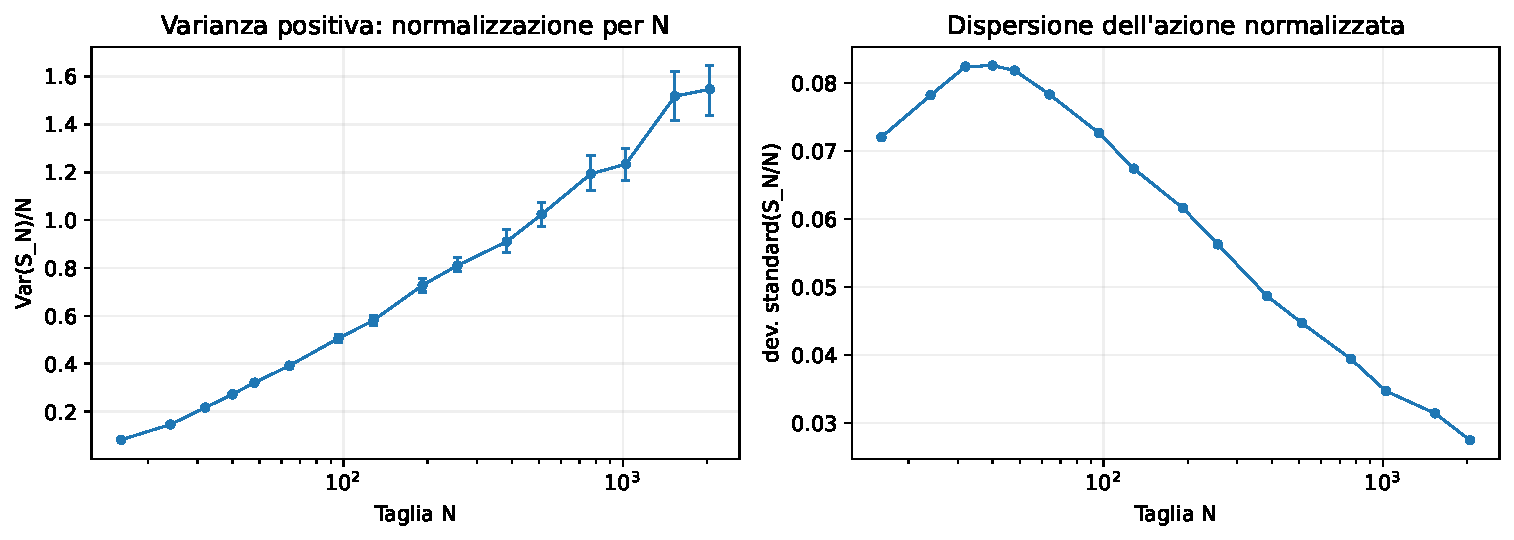
\includegraphics[width=0.96\linewidth]{r12ad_finite_fluctuations.pdf}
\caption{L'insieme dei 16 holdout preregistrati: $\mathrm{Var}(S_N)/N$ cresce nel range osservato mentre la deviazione standard di $S_N/N$ si riduce. Le barre riflettono solo il bootstrap iid. Nessun esponente asintotico e estratto dal grafico.}
\label{fig:r12ad_fluct}
\end{figure}

Le regressioni log--log, scelte \emph{prima} della produzione sulle tre finestre finite, danno pendenze $1.6994$ per $N=32$--128, $1.3211$ per $N=256$--1024 e $1.3106$ per $N=512$--2048. Le bande bootstrap al 95\% sono rispettivamente $[1.6700,1.7258]$, $[1.2743,1.3585]$ e $[1.2552,1.3704]$. Si tratta di \emph{descrittori su finestre scelte}, non di esponenti asintotici: anche gli errori bootstrap piu piccoli non controllano il bias dovuto a crossover e correzioni logaritmiche. Il bound R12ac vieta di promuovere un fit finito con esponente $>1$ a legge di potenza superlineare persistente per $N\to\infty$, ma non seleziona automaticamente $\operatorname{Var}(S_N)\sim N$, $N\ln N$ o altra struttura sub-quadratica.

\begin{figure}[htbp]
\centering
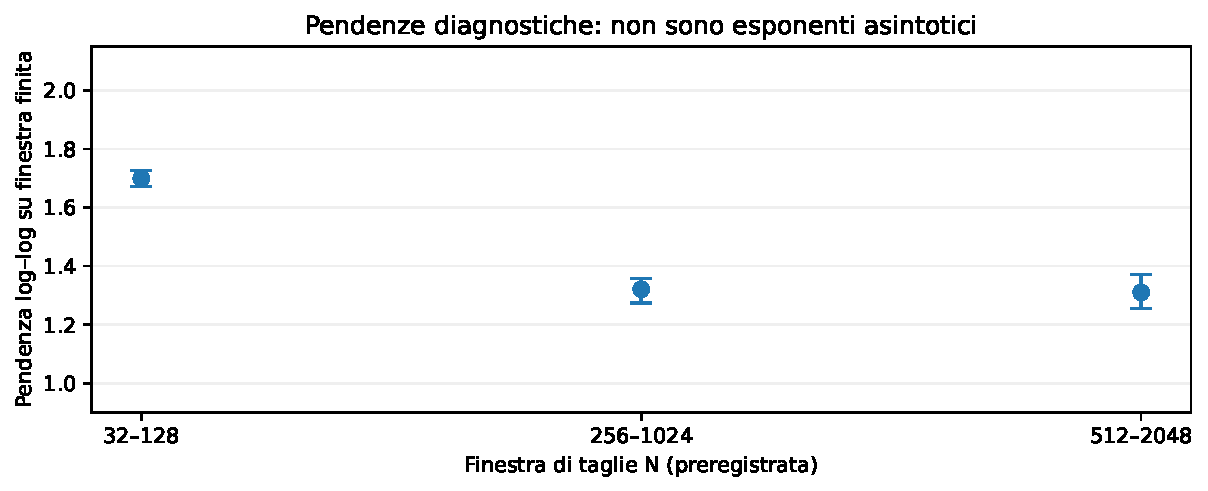
\includegraphics[width=0.88\linewidth]{r12ad_finite_window_slopes.pdf}
\caption{Pendenze log--log su finestre finite fissate nel protocollo R12ad. Le barre sono percentili bootstrap campionari, non errori sulla legge asintotica.}
\label{fig:r12ad_slopes}
\end{figure}

\subsection{Fase a $g=1$: una non-misura oltre la frontiera di precisione}

A $g=1$ il disco di Eq.~\eqref{eq:r12ad_hoeffding_disk} esclude zero soltanto per le taglie $N=16$ e $N=24$. Gia a $N=32$, nonostante la stima puntuale $|\widehat\phi_{32}(1)|\simeq0.0514$, il raggio simultaneo supera il modulo stimato; da $N=32$ a $N=2048$ tutte le taglie restano \texttt{NOT\_RESOLVED}. Le stime di fase piccole in questa regione oscillano entro la precisione statistica del campionamento diretto, senza identificare il valore reale di $|\phi_N(1)|$. Non viene calcolato ne riportato un fit affidabile della fase nella regione non risolta.

\begin{figure}[htbp]
\centering
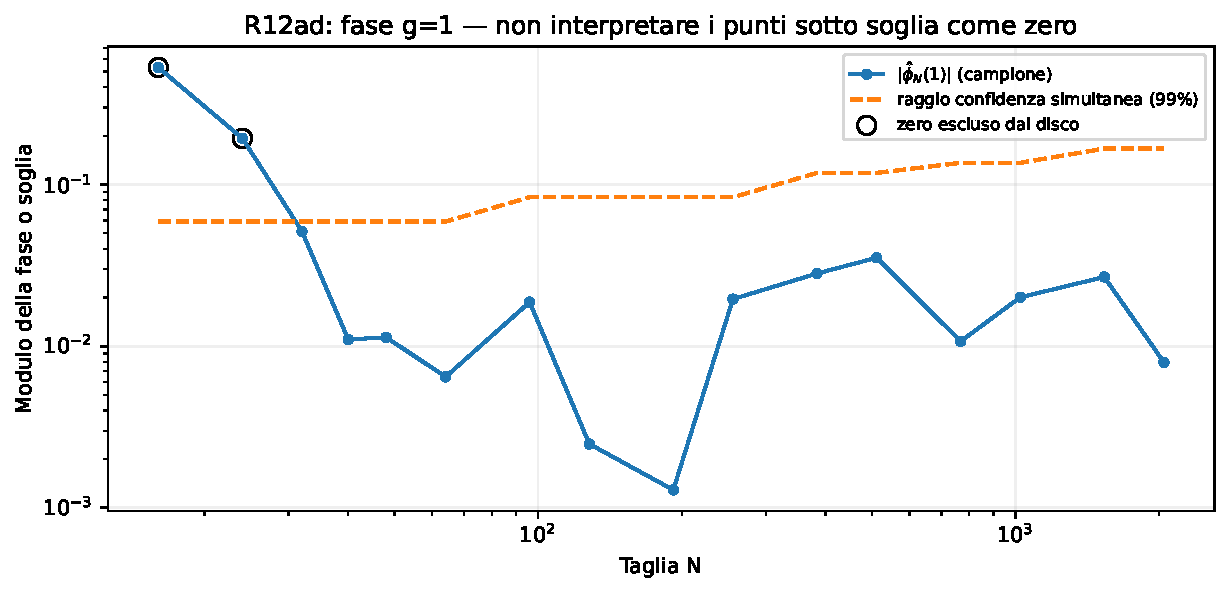
\includegraphics[width=0.91\linewidth]{r12ad_fixed_phase_resolution.pdf}
\caption{R12ad: stima del modulo della fase a coupling fissato $g=1$ e raggio del disco di confidenza valido simultaneamente al $99\%$ sull'intera griglia preregistrata. Solo due taglie superano la soglia. Ogni punto sotto la soglia e \emph{non risolto}, non una prova di fase zero.}
\label{fig:r12ad_g1}
\end{figure}

Le frequenze diagnostiche $c/\sqrt N$ sono distinte dal coupling fisico fisso: una fase accessibile a queste frequenze non autorizza a trasferire la conclusione a $g=1$. Parimenti la quasi-gaussianita empirica di alcuni momenti standardizzati non dimostra una central limit theorem. R12ad conclude che la parte con controllo rigoroso riguarda il dominio di coupling decrescente, mentre il test a coupling fisso resta soggetto alle cancellazioni note in R12v.

\subsection{Riproducibilita, verdetto e limite della strada}

Le azioni sono ricostruibili dagli array \texttt{R12AD\_RAW\_ACTIONS.npz}, dal codice \texttt{r12ad\_engine.py} e da \texttt{r12ad\_fluctuation\_phase.py}, con seed e stopping rule invariati. Il primo tentativo di esecuzione ha incontrato un limite temporale prima della scrittura degli array finali; il replay completo ha mantenuto gli stessi parametri e semi e ha introdotto soltanto checkpoint tecnici per recuperare dai timeout. La preregistrazione non e stata modificata. Le verifiche esatte, i controlli di media e le soglie di risoluzione passano. Si preservano tutti i risultati, incluso \texttt{NOT\_RESOLVED}.

\begin{quote}
\small
\noindent\status{R12AD: SHRINKING-COUPLING FOURIER BOUND DERIVED; POSITIVE 2D FINITE-$N$ VARIANCE MAPPED.}\\
\status{FIXED $g=1$ PHASE RESOLVED ONLY AT $N=16,24$; SHARP FLUCTUATIONS / 4D PATH SUM OPEN.}
\end{quote}

Il prossimo Gate \textbf{R12ae} dovra cercare una stima \emph{sharp} attraverso proiezioni Hoeffding--ANOVA, covarianze di rettangoli o una struttura equivalente, e non semplicemente moltiplicare il budget di campionamento alla fase fissa. Nessun risultato qui fornisce una sorgente tensoriale conservata, una legge cosmologica autonoma $H(t)$ o una nuova predizione osservativa. \textbf{R13 rimane BLOCCATO.}


\section{Gate R12ae: proiezione Hoeffding--ANOVA e limite inferiore alla varianza}
\label{sec:r12ae}

Il Gate R12ad ha misurato la varianza dell'azione positiva 2d su una ampia griglia, senza identificarne l'ordine asintotico \emph{sharp}. R12ae cerca un pezzo della varianza determinabile da formule esatte, non da un fit. Il protocollo \texttt{R12AE\_PREREGISTRATION.json} e stato congelato prima dei nuovi test numerici. Le valutazioni iniziali a punti selezionati con $N=2,\ldots,9$ appartengono allo sviluppo, e non vengono presentate come holdout.

\subsection{Punti iid nel quadrato e pesi di intervallo}

Siano $Z_1,\ldots,Z_N$ indipendenti e uniformi su $[0,1]^2$. Ordinando le ascisse e prendendo i ranghi delle ordinate si ottiene una permutazione uniforme, dunque esattamente il benchmark \emph{representation-weighted} dei Gate precedenti. Indichiamo con $T_N$ la somma sui rettangoli causali associati a coppie comparabili e con $K_{ij}$ il numero degli altri punti interni al rettangolo:
\begin{equation}
 S_N=4\epsilon(N-2\epsilon T_N),\qquad
 T_N=\sum_{Z_i\prec Z_j}w_\epsilon(K_{ij}),\quad \epsilon=0.21.
 \label{eq:r12ae_action}
\end{equation}
Il peso storico, ponendo $q=1-\epsilon$, e
\begin{equation}
 w_\epsilon(k)=q^k-2\epsilon kq^{k-1}
       +\tfrac12\epsilon^2k(k-1)q^{k-2},
 \label{eq:r12ae_weight}
\end{equation}
con i termini a fattoriale decrescente nulli per $k=0,1$ secondo necessita. La media $\mathbb E_0S_N=4(1-q^N)$ e l'identita di R12z, qui conservata come controllo di normalizzazione.

Per due estremi comparabili, se il rettangolo ha area $A$, il numero di altri punti $K$ e binomiale $\mathrm{Bin}(m,A)$. Due polinomi finiti governano il condizionamento:
\begin{align}
 \psi_m(A)&=\mathbb E[w_\epsilon(K)]
 =\sum_{r=0}^{m}\binom mr(-\epsilon)^r\frac{(r+1)(r+2)}2 A^r,\\
 \delta_m(A)&=\mathbb E[w_\epsilon(K+1)-w_\epsilon(K)]
 =-\epsilon\sum_{r=0}^{m}\binom mr(-\epsilon)^r
   \frac{(r+2)(r+3)}2 A^r.
 \label{eq:r12ae_psidelta}
\end{align}
Queste uguaglianze discendono espandendo $\mathbb E(1-\epsilon)^K=(1-\epsilon A)^m$ e applicando l'operatore $1+2\epsilon\partial_\epsilon+\epsilon^2\partial_\epsilon^2/2$. Il secondo polinomio e essenziale: misura esattamente l'effetto del punto marcato \emph{interno} a un intervallo che non lo ha come estremo.

\subsection{Formula condizionata esatta a ogni $N$ finito}

Fissiamo $Z_1=(x,y)$ e definiamo
\begin{align}
 F_m(z)&=\frac z2(1-\epsilon z)^m+
 \frac{1-(1-\epsilon z)^{m+1}}{2\epsilon(m+1)},
 \label{eq:r12ae_F}\\
 D_r(x)&=\frac{1-x^{r+2}-(1-x)^{r+2}}{(r+1)(r+2)},
 \label{eq:r12ae_D}\\
 G_m(x,y)&=-\frac\epsilon2\sum_{r=0}^{m}
 \binom mr(-\epsilon)^r(r+2)(r+3)D_r(x)D_r(y),\\
 I_m&=\int_0^1(1-u)(1-\epsilon u)^m\,du.
 \label{eq:r12ae_GI}
\end{align}
La funzione $F_m(XY)$ e l'integrale di $\psi_m(uv)$ su $[0,X]\times[0,Y]$: i due contributi in cui $Z_1$ e un estremo sono dunque $F_{N-2}(xy)$ e $F_{N-2}((1-x)(1-y))$. Per le coppie composte dagli altri $N-1$ punti, l'effetto di $Z_1$ internamente al rettangolo e $2G_{N-3}(x,y)$; in assenza dell'effetto interno, la media del peso di una coppia vale $I_{N-3}$. Si ottiene quindi per $N\ge3$
\begin{align}
 B_N(x,y)&=F_{N-2}(xy)+F_{N-2}((1-x)(1-y))
 +(N-2)G_{N-3}(x,y),\\
 \mathbb E[T_N\mid Z_1=(x,y)]
 &=(N-1)B_N(x,y)+\binom{N-1}{2}I_{N-3}.
 \label{eq:r12ae_condT}
\end{align}
Il caso $N=2$ e dato da $B_2=xy+(1-x)(1-y)$, senza il termine $I$. Puo essere utile esprimere l'integrale base senza quadrature:
\begin{equation}
 I_m=\frac1{\epsilon^2}\left[
 \frac{1-q^{m+2}}{m+2}-q\frac{1-q^{m+1}}{m+1}\right].
 \label{eq:r12ae_Iclosed}
\end{equation}
Usando $\mathbb E T_N=[N-(1-q^N)/\epsilon]/(2\epsilon)$, si determina $\overline B_N=\mathbb EB_N(Z_1)$ da Eq.~\eqref{eq:r12ae_condT} senza nuove assunzioni. La proiezione di primo ordine diventa
\begin{equation}
 \boxed{h_{1,N}(x,y)=\mathbb E[S_N\mid Z_1=(x,y)]-\mathbb E S_N
 =-8\epsilon^2(N-1)\,[B_N(x,y)-\overline B_N].}
 \label{eq:r12ae_h1}
\end{equation}
Questa e una formula \emph{esatta a dimensione finita}; la sua implementazione numerica usa quadrature solo per calcolare la norma $L^2$ del polinomio esplicito.

\subsection{Limite inferiore di Hoeffding e stretta positivita}

Poiche i punti $Z_i$ sono iid e $S_N$ e simmetrica rispetto alle loro etichette, i termini $h_{1,N}(Z_i)$ sono centrati e ortogonali. Pythagoras nella decomposizione Hoeffding implica esattamente
\begin{equation}
 \boxed{\mathrm{Var}_0(S_N)
 =N\mathbb E[h_{1,N}(Z_1)^2]+\mathrm{Var}_0(R_{\ge2,N})
 \ \ge N\mathbb E[h_{1,N}(Z_1)^2],}
 \label{eq:r12ae_variance_lower}
\end{equation}
ove $R_{\ge2,N}=S_N-\mathbb E S_N-\sum_i h_{1,N}(Z_i)$ e ortogonale ai termini del primo ordine. Inoltre
\begin{equation}
 h_{1,N}(0,0)-h_{1,N}(0,1)
 =-8\epsilon^2(N-1)F_{N-2}(1)<0
 \label{eq:r12ae_nonzero}
\end{equation}
per $0<\epsilon<1$; i valori di bordo distinguono due polinomi continui e mostrano che $\mathbb Eh_{1,N}^2>0$ per \emph{ogni} $N\ge2$. Questo fatto non fornisce, da solo, l'ordine asintotico della norma. Come controllo interamente simbolico, a $N=2$:
\begin{equation}
 h_{1,2}=-4\epsilon^2(2x-1)(2y-1),\qquad
 \frac{2\mathbb Eh_{1,2}^2}{\mathrm{Var}(S_2)}=\frac29.
 \label{eq:r12ae_n2}
\end{equation}

\subsection{Validazione preregistrata e confronto con la varianza storica}

La formula e confrontata con enumerazione completa per $N=3$--$8$ (incluse le $8!$ permutazioni), dodici valutazioni indipendenti \emph{high precision} dei polinomi e nove campioni iid \emph{condizionati} da $12\,000$ realizzazioni per punto a $N=8,16,32$. Tutti i confronti superano le soglie congelate; nessuna replica viene scartata. Il replay usa lo stesso $\epsilon$ di R12ad. La tavola distingue rigorosamente il numeratore, ottenuto dalla \emph{formula} di proiezione mediante quadratura, dal denominatore, \emph{stimato} nei campioni storici R12ad:

\begin{center}
\begin{tabular}{r r r r}
\toprule
$N$ & $N\mathbb E h_{1,N}^2$ & $\widehat{\mathrm{Var}}_0(S_N)$ (R12ad) & quota (\%)\\
\midrule
16 & 0.124144 & 1.3278 & 9.35\\
24 & 0.235949 & 3.5221 & 6.70\\
32 & 0.575810 & 6.9518 & 8.28\\
48 & 1.269966 & 15.4246 & 8.23\\
64 & 1.685023 & 25.1096 & 6.71\\
96 & 2.120980 & 48.6361 & 4.36\\
128 & 2.414460 & 74.4270 & 3.24\\
\bottomrule
\end{tabular}
\end{center}
A $N=8$, dove il denominatore e esatto per enumerazione completa, il primo ordine rappresenta circa il $45.91\%$ della varianza; a $N=128$ ne rappresenta circa il $3.24\%$ rispetto al denominatore campionario. La differenza e descrittiva e non prova monotonia ne un limite nullo della quota. Le verifiche della quadratura a 48 e 80 nodi coincidono entro la precisione fissata; alle taglie oltre il grado di esattezza di Gauss--Legendre questo rimane un controllo numerico, non un enclosure matematico dell'errore.

\begin{figure}[htbp]
\centering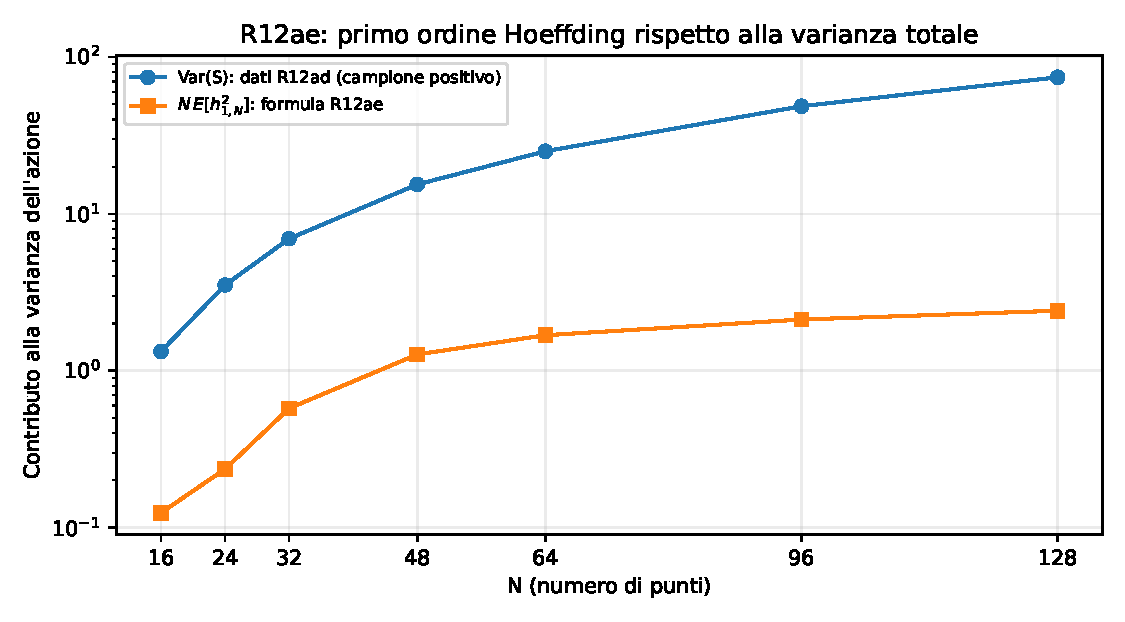
\includegraphics[width=0.95\linewidth]{r12ae_variance_projection.pdf}
\caption{R12ae: proiezione di primo ordine calcolata con formula esatta (norma valutata numericamente) e varianza totale campionaria gia misurata in R12ad. Il grafico non autorizza un esponente asintotico.}
\label{fig:r12ae_projvar}
\end{figure}
\begin{figure}[htbp]
\centering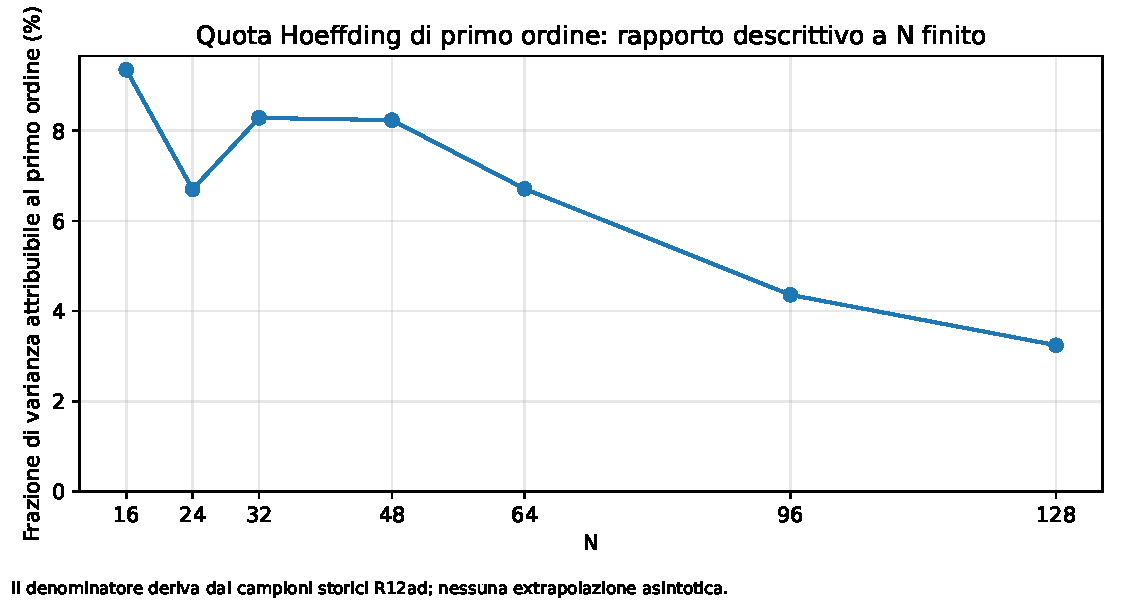
\includegraphics[width=0.95\linewidth]{r12ae_first_order_fraction.pdf}
\caption{Quota finite-$N$ attribuibile al primo ordine; il denominatore e campionario. Le quote non vanno estrapolate come una legge asintotica.}
\label{fig:r12ae_frac}
\end{figure}
\begin{figure}[htbp]
\centering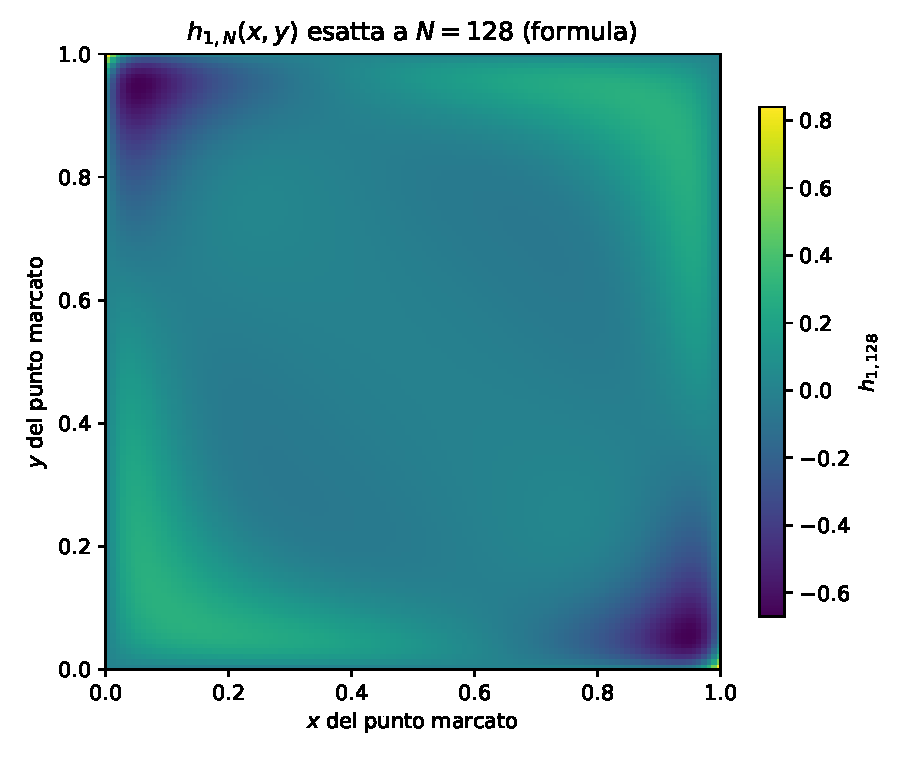
\includegraphics[width=0.82\linewidth]{r12ae_h1_spatial.pdf}
\caption{Proiezione di primo ordine $h_{1,128}(x,y)$ da Eq.~\eqref{eq:r12ae_h1}: il profilo e spazialmente non costante. Nessuna distribuzione limite e inferita dalla figura.}
\label{fig:r12ae_heat}
\end{figure}

\subsection{Verdetto R12ae e domanda aperta}

La prima proiezione e identificata senza fit e fornisce una parte \emph{rigorosa ma insufficiente} della varianza positiva. La quota residua e ortogonale al primo ordine e include componenti Hoeffding di ordine maggiore. Nessuna legge \emph{sharp} di $\mathrm{Var}(S_N)$, CLT o LDP segue dai rapporti osservati. In particolare, la stima superiore R12ac $O_\epsilon(N\log^2N)$ e distinta dalla presente disuguaglianza inferiore, e nessuna delle due controlla a $g=1$ la fase complessa.

\begin{quote}\small
\status{R12AE: FIRST HOEFFDING PROJECTION EXACT FINITE-$N$; STRICT POSITIVE VARIANCE LOWER BOUND; SHARP SCALING OPEN.}\\
\status{R12AF NEXT: SECOND-ORDER PROJECTION / RECTANGLE-COVARIANCE MECHANISM. R13 BLOCKED.}
\end{quote}

La roadmap passa alla proiezione a due punti, dove va stimata esplicitamente la parte di varianza residua, senza imporre a priori che il secondo ordine domini. R12ae concerne soltanto il benchmark positivo 2d e non equivale alla misura del path sum Lorentziano 4d.

\clearpage
\section{Cosa e gia noto e cosa resta potenzialmente nuovo}

\noindent\small\textit{Abbreviazione: STD./DERIV. = relazione standard qui derivata esplicitamente.}\normalsize\par\medskip
\begin{longtable}{p{0.39\textwidth}p{0.15\textwidth}p{0.36\textwidth}}
\toprule
Affermazione & Stato & Nota \\
\midrule
\endhead
$\dot D=HD\pm c$ per un raggio radiale in FLRW & \status{STD./DERIV.} & Conseguenza della geodetica nulla e della definizione di distanza propria. \\
\addlinespace
$\dot{\Delta D}=H\Delta D$ per due fotoni co-propaganti & \status{DERIV.} & I termini $c$ si cancellano. \\
\addlinespace
$\dot D=HD+2c$ per due fronti opposti & \status{DERIV.} & Il $2c$ e un contributo causale, non una velocita locale superluminale. \\
\addlinespace
$\dot R_H=c(1+q)$ & \status{STD./DERIV.} & Segue da $R_H=c/H$. \\
\addlinespace
$\dot R_H=2c$ nell'era radiativa & \status{STANDARD} & Per $q=1$. \\
\addlinespace
$\dot R_p=2c$ nell'era radiativa & \status{STD./DERIV.} & In quel regime $HR_p=c$ e $R_p=R_H=2ct$. \\
\addlinespace
$\alpha=HR_p/c$ e $q=(1-\alpha')/\alpha$ & \status{IDENTITA} & Nel caso piatto $\alpha=R_p/R_A$. \\
\addlinespace
$\varepsilon=HR_e/c$ e $\varepsilon'=-1-q\varepsilon$ & \status{IDENTITA} & Rapporto event horizon/apparent horizon nel caso piatto. \\
\addlinespace
Termodinamica standard su $R_A$ & \status{PASS} & Riproduce le equazioni di Friedmann, ma non seleziona $p(\rho)$. \\
\addlinespace
Chiusura autonoma di $\alpha(t)$ dalla termodinamica standard & \status{NON OTT.} & Serve contenuto fisico o legge entropica aggiuntiva. \\
\addlinespace
$\beta=H\Delta D/c$ e $d\ln\beta/d\ln a=-q$ & \status{IDENTITA} & Collega il ``fotone inseguitore'' alla storia dell'accelerazione. \\
\addlinespace
$2c$ come legge universale dell'espansione & \status{FALLITO} & Non descrive la storia cosmica nota; le interpretazioni semplici portano a radiazione permanente o coasting. \\
\addlinespace
Dinamica derivata da causalita sola & \status{NON OTT.} & Manca una chiusura indipendente per $H(t)$ o $\alpha(t)$. \\
\addlinespace
Mappa generica $S(A)\to$ Friedmann modificata & \status{DERIV.} & Eq.~\eqref{eq:entropy_friedmann_map}; richiede comunque una legge entropica come input. \\
\addlinespace
Potenza costante $S\propto A^\nu$ come chiusura universale & \status{FALLITO} & Le ere standard impongono $\nu=1$, mentre polvere accelerata richiede $\nu<1/2$ nel ramo minimale. \\
\addlinespace
Correzione logaritmica come motore tardivo minimale & \status{FALLITO} & Genera una correzione $\propto H^4$, dominante ad alta curvatura. \\
\addlinespace
Forma tipo Renyi, polvere, $C=0$ & \status{CONTROLLO} & Produce una transizione $q:1/2\to-1/4$, ma e una classe gia nota e non deriva da $c+c$. \\
\addlinespace
Landauer a saturazione sul bordo & \status{RIDONDANTE} & $E_{\rm bit}\dot N=T\dot S$: coincide con Clausius e non aggiunge una equazione. \\
\addlinespace
Saturazione Bekenstein su $R_A$ & \status{CONTROLLO} & Ricostruisce $H^2=8\pi G\rho/3$ nel caso piatto ma non determina $p(\rho)$. \\
\addlinespace
Holographic equipartition & \status{RIFORMULAZ.} & Recupera l'equazione di accelerazione usando gia $\rho+3p$ nel bulk. \\
\addlinespace
Flusso informazionale standard come chiusura di $\alpha$ & \status{NON OTT.} & Nessuno dei principi testati determina autonomamente la storia cosmica. \\
\addlinespace
$\rho\propto R_p^{-2}$ come sorgente totale a coefficiente costante & \status{FALLITO} & Impone $\alpha=C$ e quindi $q=1/C>0$: una sola era di potenza, nessuna transizione. \\
\addlinespace
Combinazione totale $A/R_p^2+B/R_A^2$ con $A,B$ costanti & \status{NO-GO RIST.} & Friedmann forza ancora $\alpha$ costante, salvo il ramo tautologico $A=0,B=1$. \\
\addlinespace
$\rho\propto R_e^{-2}$ & \status{BENCHMARK} & Puo accelerare ma usa il future event horizon; non deriva dal solo passato causale. \\
\addlinespace
$\rho\propto\eta^{-2}$ (conformal age) & \status{BENCHMARK} & Puo crescere tardivamente; coincide con new agegraphic DE e richiede una motivazione microfisica aggiuntiva. \\
\addlinespace
Toy $R_p^{-2}+R_e^{-2}$, $C=1$ & \status{FALLITO} & Interpola $q:1\to-1$ ma attraversa troppo rapidamente $q=1/2$ per produrre una lunga era materiale. \\
\addlinespace
$\eta^{-2}$ derivata dalla sola struttura nulla FLRW & \status{NON OTT.} & $\eta$ cambia sotto la normalizzazione $a\to\lambda a$; serve una reference scale o nuova fisica. \\
\addlinespace
$\rho_X=\rho_cF(\alpha,\alpha',q,\ldots)$ senza nuova scala & \status{NO-GO RIST.} & In una esatta era di potenza gli argomenti sono costanti e quindi $\Omega_X$ resta costante: tracking inevitabile. \\
\addlinespace
$\rho_X\propto L_*^{n-2}R_p^{-n}$ con una nuova scala & \status{PASS PARZ.} & Per $n<2$ rompe il tracking; la scala e l'esponente restano input non derivati. \\
\addlinespace
$n=1$: $\rho_X\propto(L_*R_p)^{-1}$ & \status{BENCHMARK} & Produce takeover e attrattore $q\to-1/2$, ma coincide con Tsallis HDE a $\delta=3/2$. \\
\addlinespace
Interazione $Q$ con $\rho_p\propto R_p^{-2}$ & \status{NO-GO RIST.} & Se $q<0$, l'identita geometrica forza $\Omega_p'<0$: l'eventuale accelerazione e guidata dall'interazione, non dal takeover di $R_p^{-2}$. \\
\addlinespace
Flusso naturale del particle horizon & \status{RIDONDANTE} & $4\pi R_p^2c\rho$ e il termine di sweep di un volume mobile; inserirlo come $Q$ locale conterebbe due volte lo stesso trasporto. \\
\addlinespace
Memoria $-\Box U=1$, $\rho\propto U^{-1}$ & \status{TRACKER} & In $a\propto t^p$, $U\propto t^2$ e la densita scala come $H^2$. \\
\addlinespace
Memoria $X=-\Box^{-1}R$ & \status{PASS PARZ.} & Puo crescere secolarmente, ma una funzione/coupling aggiuntiva e necessaria per trasformarla in dinamica. \\
\addlinespace
Raychaudhuri nulla FLRW & \status{RIFORMULAZ.} & Ricostruisce $\dot H-k/a^2=-4\pi G(\rho+p)$; non fornisce una chiusura indipendente. \\
\addlinespace
Raggio uscente su $R_A=c/H$ (piatto) & \status{STD./DERIV.} & $\dot R_+=2c$ esatto; il ramo entrante ha $\dot R_-=0$. Il movimento dell'orizzonte e invece $c(1+q)$. \\
\addlinespace
Selezione di $\Lambda$ dalla sola prima luce & \status{NO-GO RIST.} & Il focusing nullo dipende da $\rho+p$ ed e cieco a $p=-\rho$; l'integrazione lascia una costante non determinata. \\
\addlinespace
Entanglement equilibrium / unimodularita & \status{NON CHIUDE} & Ricostruiscono o ricodificano il settore cosmologico, ma il valore di $\Lambda$ resta dato globale, di stato o boundary condition. \\
\addlinespace
Sequestering globale & \status{PASS PARZ.} & Neutralizza la sensibilita all'energia del vuoto, ma introduce vincoli globali e nella forma originale dipende dal quattro-volume totale/futuro. \\
\addlinespace
$\Lambda_{\rm rms}\propto V_4[J^-]^{-1/2}$ causal-set & \status{PASS PARZ.} & Solo passato causale e scala naturale, ma e stocastico; nelle ere di potenza traccia $H^2$ e richiede ampiezza/microfisica aggiuntiva. \\
\addlinespace
Kernel $\mathcal C=V(P_x\cap P_y)/\sqrt{V_xV_y}$ & \status{DERIV. TOY} & Segue da contributi iid condivisi per elemento causale; fissa correlazioni geometriche senza imporre omogeneita, ma non deriva la dinamica quantistica microscopica. \\
\addlinespace
$\Lambda(x)g_{\mu\nu}$ con materia separatamente conservata & \status{BLOCCO} & Bianchi forza $\partial_\nu\Lambda=0$; serve un settore compensatore, scambio energetico o una modifica/nonlocalita covariante non ancora selezionata. \\
\addlinespace
Proiezione trasversa retarded di $\Lambda g_{\mu\nu}$ & \status{PASS ESISTENZA} & Produce una sorgente conservata e causale a livello efficace, ma richiede Green function, boundary conditions/soluzioni omogenee e non e unica. \\
\addlinespace
Fluido efficace con $\rho_s=\Lambda/(8\pi G)$ & \status{PASS BG} & Se la materia e separatamente conservata, $p_s=-\rho_s-\dot\rho_s/(3H)$; non e piu vuoto e l estensione perturbativa non e selezionata. \\
\addlinespace
Vuoto stocastico $p=-\rho$ interagente & \status{PASS PARZ.} & Bianchi fissa il transfer totale $\sum_iQ_i^\nu=\nabla^\nu\rho_s$, ma non la ripartizione tra specie ne la microfisica del trasferimento. \\
\addlinespace
Campo overlap grezzo differenziabile & \status{FALLITO} & La cuspide lineare del kernel implica varianza del quoziente incrementale $\propto1/\Delta$; serve coarse-graining, stochastic calculus o smoothing nonlocale. \\
\addlinespace
Noise tensoriale conservato da solo overlap scalare & \status{NO-GO RIST.} & In Minkowski restano almeno spettri trasversi spin--2 e spin--0 indipendenti; l'overlap non seleziona la polarizzazione tensoriale. \\
\addlinespace
Toy causal-set con marks tensoriali & \status{FATTORIZZ.} & Il volume di overlap fissa il prefattore geometrico, mentre la covarianza tensoriale $\Sigma_{\mu\nu\rho\sigma}$ resta dato microscopico. \\
\addlinespace
Azione diffeo-invariante con soli gradi dinamici on-shell & \status{PASS STRUTT.} & La Ward identity rende conservata la sorgente metrica, ma non determina la sua covarianza stocastica. \\
\addlinespace
Scalare stocastico esterno $\lambda(x)$ nell'azione & \status{FALLITO} & $T_{\mu\nu}=-\lambda g_{\mu\nu}$ ha divergenza $-\partial_\nu\lambda$: l'identita di Ward include la variazione della sorgente esterna. \\
\addlinespace
Seconda variazione / azione quadratica covariante & \status{NON UNICA} & Ward consente form factor indipendenti spin--2 e spin--0; la simmetria non fissa $F_2/F_0$. \\
\addlinespace
Azione BDG causal-set & \status{BENCHMARK} & Il primo cumulante tende a Einstein--Hilbert piu joint boundary, ma non determina il secondo cumulante/noise kernel; lo smearing noto introduce una nonlocality scale. \\
\addlinespace
Formalismo del secondo cumulante BDG & \status{PASS FORMAL.} & La varianza viene ridotta a una matrice di correlazioni/integrali geometrici; l'asintotica esplicita Minkowski/FLRW resta da valutare. \\
\addlinespace
Matching Everpresent $\mathrm{Var}(S)\propto N^\gamma$ & \status{CRITERIO} & $\Lambda_{\rm rms}\propto N^{\gamma/2-1}$: il comportamento $N^{-1/2}$ richiede esattamente $\gamma=1$. \\
\addlinespace
Mesoscale $\ell_k$ da smearing causal-set & \status{NON SELEZ.} & A $\ell_k$ fisica fissata lo smearing sopprime le fluttuazioni nel continuum; una sorgente finita richiede running/critical scaling non ancora derivato. \\
\addlinespace
Pilot R12m: controllo sintetico & \status{PASS} & Recupera $\gamma=0.9930$ con CI 95\% $[0.9777,1.0088]$, validando l estimatore preregistrato. \\
\addlinespace
Pilot R12m: sprinkling fixed-$N$ & \status{REJECTS $\gamma=1$} & $\gamma_{\rm spr}=1.8574$, CI $[1.8401,1.8754]$ sulla griglia congelata $N=24$--$96$. \\
\addlinespace
Pilot R12m: Gibbs continuum-like & \status{REJECTS $\gamma=1$} & $\gamma_{\rm G}=1.6368$, CI $[1.5657,1.7209]$, $R^2=0.9906$, min ESS $430$; non e $\gamma_Q$. \\
\addlinespace
R12n: exact Lorentzian characteristic function, $N=4$--$10$ & \status{CONSIST. EXT. REP} & $\gamma_Q^{\rm rep}=1.1807$, $R^2=0.9932$; endpoint fit $1.1893$ e $1.0928$; $\min|\phi_N(1)|=0.7775$ (sign problem mild). \\
\addlinespace
R12o: estensione MC Lorentziana, $N=12$--$64$ & \status{INCONCL.} & Replay esatto PASS; quality-pass solo $N=12$--$24$; local slope $1.61$--$1.93$; da $N=32$ cumulante non risolto e da $N=48$ fase non risolta. \\
\addlinespace
R12p: ricostruzione cumulante/Fourier & \status{METHOD FAIL} & Exact $N=8$--$10$ e direct fino a $N=20$ PASS; a $N=24$ errore su $\kappa_2$ $\simeq65\%$ e troncature $K=8,10,12$ instabili. Nessuna estensione autorizzata. \\
\addlinespace
R12q: DOS globale Wang--Landau/multicanonica & \status{METHOD FAIL} & Accuratezza PASS quando converge (errori su $\kappa_2$ tipicamente $<3.3\%$), ma replica gate fallisce: $2/4$ a $N=9$ e $1/4$ a $N=12$ contro minimo $3/4$. Nessun $N>24$. \\
\addlinespace
R12r: LLR histogram-free / log-DOS slopes & \status{METHOD FAIL} & Exact $N=8$ PASS; replica gate fallisce a $N=9$ e $N=10$ ($1/3$ valida, minimo $2/3$). Direct $N=12$--$24$ ed estensione non eseguite. \\
R12s: soft-window umbrella / replica exchange / MBAR & \status{METHOD FAIL} & Exact $N=8$--$10$ PASS con $3/3$ repliche; direct $N=12,16,20$ PASS; $N=24$ FAIL di poco ($5.84\%$ su $\phi$, $15.33\%$ su $\kappa_2$). Estensione non eseguita. \\
\addlinespace
R12t: stratificazione indipendente dei momenti complessi & \status{VALIDATO / INCONCL.} & Exact e direct fino a $N=24$ PASS con $3/3$ repliche; estensione autorizzata. $N=32$ conserva $2/3$ repliche coerenti, $N=40$ $1/3$, $N=48,64$ $0/3$; solo tre taglie utili per lo scaling, quindi nessun fit di $\gamma$. \\
R12u: Lehmer-ANOVA control variates & \status{VALIDATO / INCONCL.} & Exact/direct fino a $N=24$ PASS. La riduzione di varianza decade da $\sim70\%$ a piccole taglie a zero attorno a $N=32$; solo $1/3$ replica a $N=32$ e nessuna a $N=40,48,64$ supera il quality gate, quindi nessun fit di $\gamma$. \\
\addlinespace
R12v: cost law / efficiency frontier & \status{DERIVATO} & Per il phase estimator diretto $\mathrm{RelMSE}=(1-|\phi|^2)/(M|\phi|^2)$ e R12o segue la previsione. La delta-method di $\kappa_2$ sposta il costo a $\sim1.66\times10^6$ campioni a $N=32$ e $\sim1.15\times10^8$ a $N=40$ per il target 15\%. Nessun bound universale su metodi strutturati viene rivendicato. \\
\addlinespace
R12w: scaled DOS / surrogate sestico troncato & \status{LOC. VALID. / GLOB. RITIRATO} & Holdout fresco: $\mathrm{Var}(S)\propto N^{2.004}$, $X_N=(S-4)/N$ quasi collassa e $\phi_N(g)=e^{4ig}\widehat f_N(gN)$. Exact/direct validano il surrogate sulla finestra implementata; R12x ritira la sua interpretazione globale. \\
\addlinespace
R12x: audit analitico / truncated moment identifiability & \status{SADDLE NON AUTORIZZATO} & $9/33$ continuazioni sestiche hanno modi remoti dominanti; gli stessi momenti $m_0\ldots m_6$ permettono quasi ogni fase ad alta frequenza gia a $N=48$--$64$. Prossimo ramo: limite di permuton/struttura combinatoria. \\
\addlinespace
R12y: permuton-only action limit & \status{NO-GO GLOBALE} & Due successioni verso lo stesso permuton uniforme danno $\lim S/N=1.2409009$ e $0.5766429$; i conteggi degli intervalli microscopici non sono determinati dalla topologia debole. Non esclude convergenza tipica ne LDP congiunte. \\
\addlinespace
R12z: $\mathbb E[N_k]/N$ e $\mathbb E[S_N]$ & \status{IDENTITA ESATTA} & La media del profilo grezzo cresce come $\ln N$ a $k$ fisso, ma $\mathbb E[S_N]=4[1-(1-\epsilon)^N]$; il profilo centrato e una identita finita, tightness/LDP congiunta non dimostrate. \\
\addlinespace

R12aa: curvatura discreta e cutoff $K_N=O(\ln N)$ & \status{DERIVATO} & Azione riscritta in seconde differenze; $\mathbb E[\mathcal C_N(k)]$ esatta, errore normalizzato uniforme per cutoff crescente. Nessuna LDP derivata. \\
\addlinespace
R12aa: cutoff $K$ fisso, uniforme su tutte le permutazioni & \status{NO-GO} & Costruzione a tre blocchi, $N_k=m^2$, coda normalizzata diverge. Non esclude tightness sotto la misura uniforme. \\
\addlinespace
R12ab: covarianze di $\mathcal C_N(k)$, misura positiva & \status{DERIVATO / LIMITE APERTO} & Rappresentazione finite-$N$ esatta tramite coppie di intervalli; enumerazione indipendente fino a $N=6$, holdout fino a $N=1024$. Il criterio $L^2\Leftrightarrow Q_{N,K_N}\to0$ e rigoroso, ma l'asintotica della forma quadratica non e dimostrata. \\
\addlinespace
R12ac: controllo Efron--Stein nel benchmark positivo 2d & \status{TEOREMA $L^2$} & $\mathrm{Var}_0(S_N)=O_\epsilon(N\ln^2 N)$; concentrazione di $S_N/N$ e $Q_{N,K_N}\to0$ con cutoff logaritmico. Non chiude la fase Lorentziana. \\
\addlinespace
R12ad: finestra Fourier e fase del benchmark positivo & \status{DERIVATO / FINITE-$N$} & Controllo rigoroso solo per $g_N=o([\sqrt N(1+\ln N)]^{-1})$; holdout $N\le2048$ e fase $g=1$ statisticamente risolta a $N=16,24$ soltanto. Sharp order ancora aperto. \\
\addlinespace
R12ae: prima proiezione Hoeffding del toy positivo 2d & \status{FORMULA ESATTA / LIMITE APERTO} & $h_{1,N}(z)$ e polinomio esplicito, $\mathrm{Var}_0(S_N)\ge N\mathbb E h_{1,N}^2>0$; piccola quota rispetto alla varianza R12ad a $N=128$. Nessun esponente sharp derivato. \\

\addlinespace
R12af: seconda proiezione Hoeffding del toy positivo 2d & \status{FINITO ESATTO / SHARP APERTO} & Formula $h_{2,N}$ esatta e $\mathrm{Var}(S_N)=P_1+P_2+\mathrm{Var}(R_{\ge3})$; 30/30 test PASS. Fra $N=16$ e $48$, $P_1+P_2$ e circa 67--76\% della varianza campionaria storica. Nessun esponente limite inferito. \\
\addlinespace
R12ag: terza proiezione Hoeffding del toy positivo 2d & \status{FINITO ESATTO / RESTO APERTO} & Formula $h_{3,N}$ esatta (con tre marcati interni), $P_3$ stimato da quattro scramble QMC, 31/31 controlli PASS; una quarta differenza non nulla implica $P_{4,4}>0$. Nessuno sharp exponent o limite di $V_{\ge4,N}$ derivato. \\ 
\addlinespace
R12ah: resampling e certificato del residuo superiore & \status{TEOREMA FINITO / SHARP APERTO} & Identita $C_N(p)=\sum_rp^rP_{r,N}$; per $p=1/2$, $B_N\le V_{\ge4,N}\le16B_N/15$ per aspettative esatte. 125/125 controlli PASS; nuove stime finite con disaccordi puntuali dai residui storici. Nessun limite relativo dimostrato. \\
\addlinespace
R12ai: audit e tensore da overlap su Minkowski 4d & \status{PASS PIATTO / PONTE BLOCC.} & Kernel Gram positivo e tensore conservato in senso distribuzionale su sfondo piatto; sorgente curved on-shell, spin--2, risposta, misura Lorentziana e limite 4d non derivati. R13 bloccato. \\
\addlinespace
R12aj: definizione di un candidato microdinamico 4d & \status{PROSSIMO} & Richiede un singolo ensemble, misura, azione, sorgente metrica, Ward, risposta e limite. Stop se il candidato non e specificabile senza input post hoc. \\
\addlinespace
Cumulante Lorentziano asintotico/full 4d $\gamma_Q$ & \status{APERTO} & R12n e small-$N$, 2d e representation-weighted; non autorizza il passaggio al path sum non etichettato 4d. \\
\addlinespace
Nuova teoria cosmologica falsificabile & \status{APERTA} & Richiede una legge aggiuntiva con predizioni diverse da GR/\LCDM. \\
\bottomrule
\end{longtable}

\section{Gate R12af: secondo ordine Hoeffding--ANOVA del benchmark positivo 2d}
\label{sec:r12af}

Il Gate R12ae ha ricavato la prima proiezione $h_{1,N}(z)$, ma essa non determina la varianza totale. R12af isola il contributo di secondo ordine \emph{senza supporre indipendenza dei rettangoli che condividono punti}. Il protocollo \texttt{R12AF\_PREREGISTRATION.json} e stato congelato prima dei nuovi confronti condizionati e delle quadrature sulla norma del secondo ordine. Le poche valutazioni puntuali effettuate durante la derivazione sono classificate come \emph{development} e non come holdout.

\subsection{Polinomi con zero, uno o due punti interni forzati}

Restiamo nel benchmark \emph{positive, representation-weighted, 2d}, con $Z_i$ iid uniformi su $[0,1]^2$, $\epsilon=0.21$ fissato e l'azione di Eq.~\eqref{eq:r12ae_action}. Per un rettangolo causale di area $A$, siano $B\sim\mathrm{Bin}(m,A)$ e $\Delta w(k)=w(k+1)-w(k)$. Definiamo
\begin{equation}
 W_m^{(j)}(A)=\mathbb E[\Delta^j w_\epsilon(B)],\qquad j=0,1,2.
 \label{eq:r12af_Wdef}
\end{equation}
L'operatore $1+2\epsilon\partial_\epsilon+\frac12\epsilon^2\partial_\epsilon^2$ applicato a $(1-\epsilon)^k$ restituisce il peso $w_\epsilon(k)$ di R12ae. Per la variabile binomiale otteniamo i tre polinomi esatti
\begin{equation}
 \boxed{W_m^{(j)}(A)=(-\epsilon)^j\sum_{r=0}^m\binom mr(-\epsilon)^r\,
 \frac{(r+j+1)(r+j+2)}{2}\,A^r.}
 \label{eq:r12af_Wpoly}
\end{equation}
$W^{(0)}$ e $W^{(1)}$ coincidono con $\psi_m$ e $\delta_m$ della sezione precedente. Il nuovo $W^{(2)}$ descrive \emph{entrambi} i punti marcati interni allo stesso rettangolo.

\subsection{Condizionamento su due punti: tutti i termini di sovrapposizione}

Scriviamo $u\prec v$ per l'ordine stretto in entrambe le coordinate e $R(u,v)$ per il rettangolo aperto. Per $z=(x,y)$ e $z'=(x',y')$ definiamo, con integrali su $[0,1]^2$:
\begin{align}
 E_m(z)&=\int_{v\prec z\,\lor\,z\prec v} W_m^{(0)}(A(z,v))\,dv,\\
 I_m&=2\int_{u\prec v}W_m^{(0)}(A(u,v))\,du\,dv,\\
 J_m(z)&=\int_{u\prec z\prec v}W_m^{(1)}(A(u,v))\,du\,dv,\\
 J_m^{(2)}(z,z')&=\int_{u\prec z,\,z'\prec v}W_m^{(2)}(A(u,v))\,du\,dv.
 \label{eq:r12af_integrals}
\end{align}
Il fattore $2$ in $I_m$ deriva dalle due assegnazioni possibili degli estremi liberi. Definiamo inoltre il termine \emph{misto} $M_m(z,z')$ come somma di due integrali su un punto libero $v$: il primo e su $v$ comparabile a $z$ con $z'\in R(z,v)$, e il secondo scambia $z,z'$, entrambi pesati da $W_m^{(1)}(A)$.

La media condizionata a un punto di R12ae equivale a
\begin{equation}
 T_{1,N}(z):=\mathbb E[T_N\mid Z_1=z]=(N-1)E_{N-2}(z)
 +\binom{N-1}{2}[I_{N-3}+2J_{N-3}(z)].
 \label{eq:r12af_T1}
\end{equation}
La somma delle tre classi di coppie (entrambi gli estremi marcati; uno marcato; nessuno marcato) fornisce, per $N\ge4$,
\begin{align}
 T_{2,N}(z,z')&:=\mathbb E[T_N\mid Z_1=z,Z_2=z']\\
 &=\mathbf 1_{z\sim z'}W_{N-2}^{(0)}(A(z,z'))\notag\\
 &\quad +(N-2)[E_{N-3}(z)+E_{N-3}(z')+M_{N-3}(z,z')]\notag\\
 &\quad +\binom{N-2}{2}[I_{N-4}+2J_{N-4}(z)+2J_{N-4}(z')+2J_{N-4}^{(2)}(z,z')].
 \label{eq:r12af_T2}
\end{align}
L'indicatore $z\sim z'$ significa che i due punti sono comparabili. Per $N=2,3$ si omettono le classi di coppie impossibili. Anche se $z,z'$ sono incomparabili, $J^{(2)}$ puo non essere nullo: entrambi possono giacere dentro lo stesso rettangolo formato da due punti liberi. Eliminare questo termine produrrebbe una proiezione errata.

Tutti gli integrali sono somme \emph{finite} di potenze grazie a Eq.~\eqref{eq:r12af_Wpoly}. Per esempio, per $\ell=\min(a,b)$, $h=\max(a,b)$,
\begin{equation}
 D_r(a,b)=\frac{1-(1-\ell)^{r+2}-h^{r+2}+(h-\ell)^{r+2}}{(r+1)(r+2)}
 \label{eq:r12af_Dtwo}
\end{equation}
permette di scrivere $J_m^{(2)}(z,z')=\sum_r c_{m,r}^{(2)}D_r(x,x')D_r(y,y')$, ove $c_{m,r}^{(2)}$ e il coefficiente di $A^r$ in $W_m^{(2)}$. Gli altri integrali sono trattati analogamente nei sorgenti riproducibili: \texttt{r12af\_projection.py} usa aritmetica \texttt{longdouble}, mentre \texttt{r12af\_fast.py} usa le stesse formule in una quadratura compilata.

\subsection{Proiezione degenere e limite inferiore alla varianza}

Indicando con $\mu_T=\mathbb E T_N$ il valore esatto ottenuto in R12z, otteniamo la formula condizionata di secondo ordine
\begin{equation}
 \boxed{h_{2,N}(z,z')=-8\epsilon^2[T_{2,N}(z,z')-T_{1,N}(z)-T_{1,N}(z')+\mu_T].}
 \label{eq:r12af_h2}
\end{equation}
Per la torre delle aspettative e la centratura di $h_1$, $\mathbb E_{Z'}h_{2,N}(z,Z')=0$ per quasi ogni $z$. La proiezione e percio ortogonale a ogni $h_1(Z_i)$; coppie diverse di $h_2$ sono ortogonali anche se condividono uno dei due indici, per la stessa degenerazione condizionata. La decomposizione di Hoeffding porta dunque alla \emph{identita}, non solo alla disuguaglianza,
\begin{equation}
 \boxed{\mathrm{Var}_0(S_N)=\underbrace{N\mathbb E h_{1,N}^2}_{P_{1,N}}
 +\underbrace{\binom N2\mathbb E h_{2,N}^2}_{P_{2,N}}
 +\mathrm{Var}_0(R_{\ge3,N}),\quad \mathrm{Var}_0(R_{\ge3,N})\ge0.}
 \label{eq:r12af_var_decomposition}
\end{equation}
Il caso $N=2$ e un controllo algebrico completo. Con $p(z)=xy+(1-x)(1-y)$ e $C(z,z')$ indicatore della comparabilita,
\begin{align}
 h_{2,2}(z,z')&=-8\epsilon^2[C(z,z')-p(z)-p(z')+\tfrac12],\\
 \mathrm{Var}(S_2)&=16\epsilon^4,\quad P_{1,2}=\tfrac{32}{9}\epsilon^4,\quad
 P_{2,2}=\tfrac{112}{9}\epsilon^4.
 \label{eq:r12af_N2}
\end{align}
Quindi $P_{1,2}/\mathrm{Var}(S_2)=2/9$ e $P_{2,2}/\mathrm{Var}(S_2)=7/9$: il residuo e esattamente nullo.

\subsection{Validazione prospettica e quantificazione finite-$N$}

La validazione preregistrata chiude con \textbf{30/30 PASS}: identita $N=2$, tre integrali geometrici indipendenti a $N=3$, enumerazione completa delle $N!$ permutazioni per $N=2,\ldots,8$, sei confronti della quadratura a $14$ e $18$ nodi per $N\le16$, e dodici simulazioni condizionate (tre coppie geometriche ciascuna a $N=4,8,16,32$, $12\,000$ realizzazioni per cella). Non sono state eliminate repliche. La prima emissione del report JSON ha richiesto una correzione tecnica del serializzatore \texttt{numpy.bool\_}; il seed, i test e le soglie non sono cambiati e il replay e stato effettuato dal seme congelato. I controlli supplementari a $24$ e $28$ nodi per $N=24,32,48$ sono diagnostici successivi e non vengono presentati come prospettici.

\begin{center}\small
\begin{tabular}{r r r r r}
\toprule
$N$ & $P_{1,N}$ & $P_{2,N}$ & $\mathrm{Var}(S_N)$ & $(P_1+P_2)/\mathrm{Var}$\\
\midrule
2 & 0.006915 & 0.024202 & 0.031117\textsuperscript{E} & 100.0\%\\
3 & 0.029491 & 0.049473 & 0.081749\textsuperscript{E} & 96.6\%\\
4 & 0.062901 & 0.068799 & 0.141061\textsuperscript{E} & 93.4\%\\
8 & 0.174209 & 0.128565 & 0.379463\textsuperscript{E} & 79.8\%\\
16 & 0.124144 & 0.766492 & 1.327803\textsuperscript{MC} & 67.1\%\\
24 & 0.235949 & 2.345249 & 3.522062\textsuperscript{MC} & 73.3\%\\
32 & 0.575810 & 4.617158 & 6.952288\textsuperscript{MC} & 74.7\%\\
48 & 1.269966 & 10.498332 & 15.424605\textsuperscript{MC} & 76.3\%\\
\bottomrule
\end{tabular}
\end{center}
\noindent\textsuperscript{E} Denominatore esatto da enumerazione completa; \textsuperscript{MC} denominatore \emph{campionario storico} R12ad (digest verificato), non un nuovo holdout. Anche i valori $P_1,P_2$ sono valutati numericamente come integrali delle proiezioni esatte. Le percentuali oltre $N=8$ non sono dunque esatte e non autorizzano extrapolazioni.

\begin{figure}[htbp]
\centering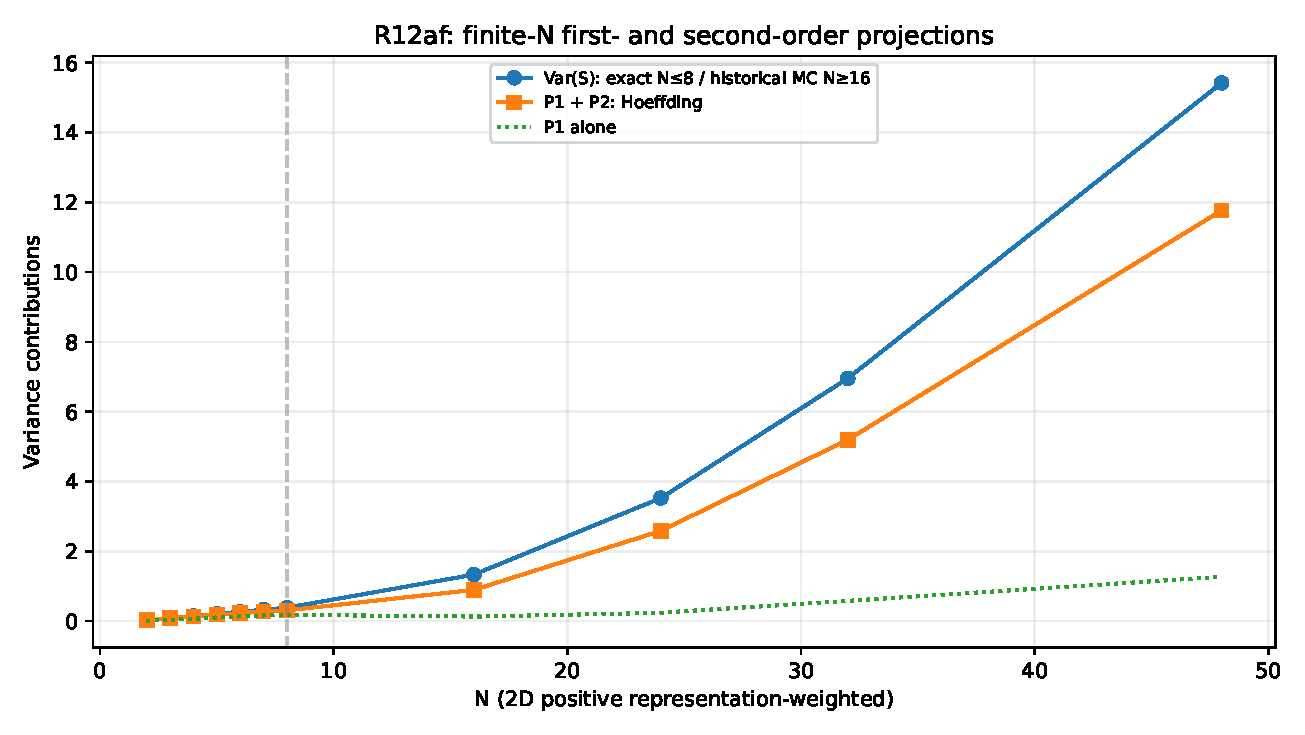
\includegraphics[width=0.90\linewidth]{r12af_variance_decomposition.pdf}
\caption{Proiezioni $P_1$ e $P_1+P_2$ a confronto con la varianza esatta per $N\le8$ e con il benchmark campionario storico a $N\ge16$. La disuguaglianza teorica riguarda la varianza vera, non un singolo stimatore Monte Carlo.}
\label{fig:r12af_var}
\end{figure}
\begin{figure}[htbp]
\centering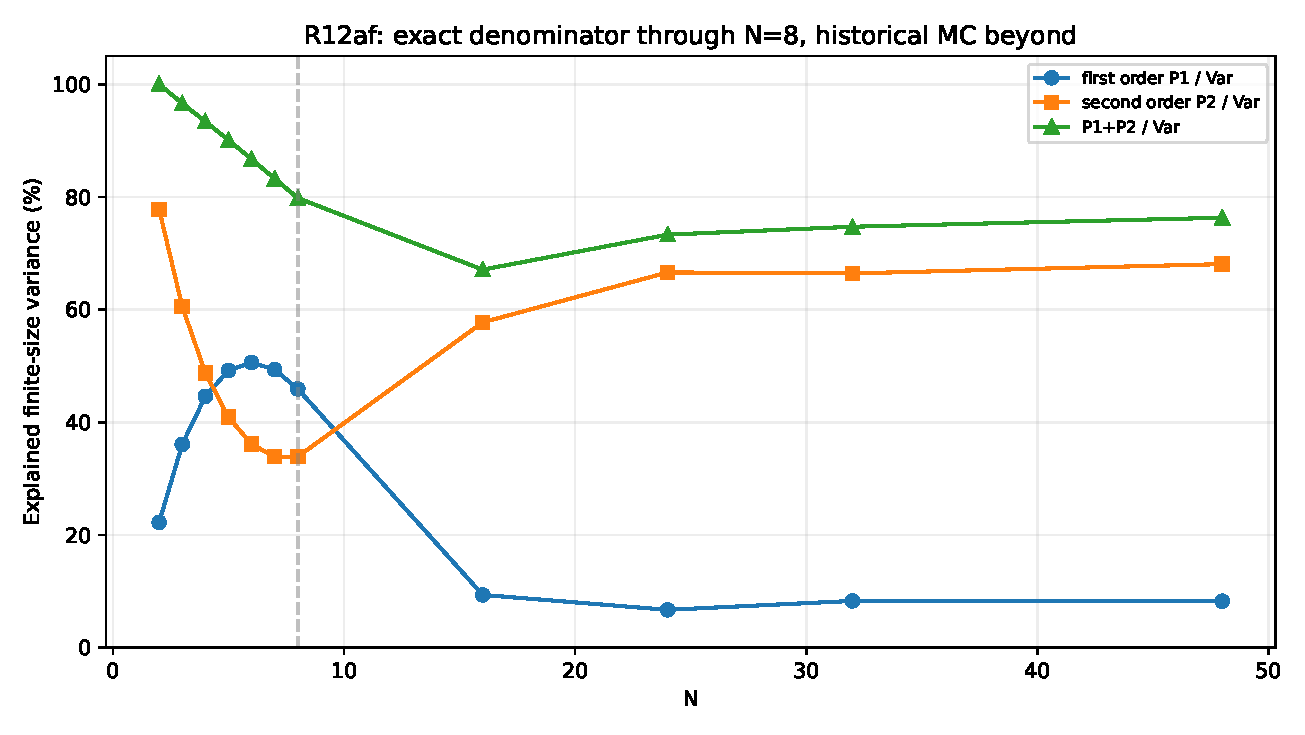
\includegraphics[width=0.86\linewidth]{r12af_projection_fractions.pdf}
\caption{Frazioni di varianza spiegate: il secondo ordine e una componente importante alle taglie studiate, ma non e dimostrato che sia dominante asintoticamente.}
\label{fig:r12af_fracs}
\end{figure}
\begin{figure}[htbp]
\centering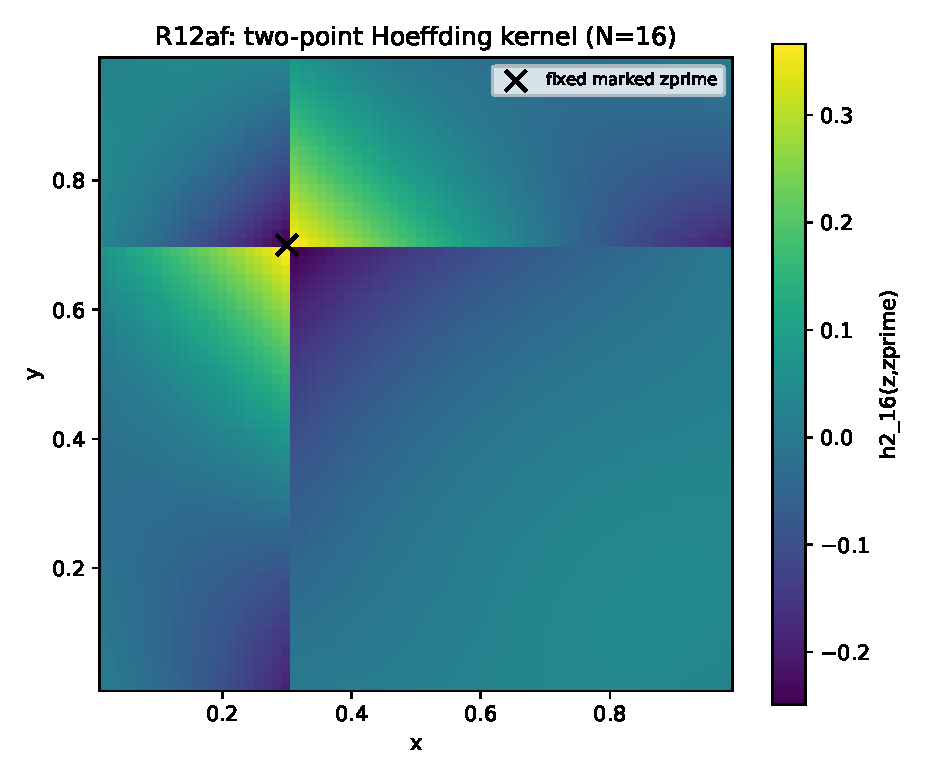
\includegraphics[width=0.72\linewidth]{r12af_h2_slice.pdf}
\caption{Sezione del kernel $h_{2,16}(z,z')$ a $z'=(0.3,0.7)$. La distinzione fra regioni comparabili e incomparabili deriva dall'ordine causale dei punti, non da parametri del fit.}
\label{fig:r12af_slice}
\end{figure}

\subsection{Verdetto e blocker ancora aperto}

\begin{quote}\small
\status{R12AF: SECOND HOEFFDING PROJECTION EXACT FINITE-$N$ AND VALIDATED; SECOND ORDER EXPLAINS A SUBSTANTIAL FINITE-SIZE FRACTION.}\\
\status{RESIDUAL $\ge3$ AND SHARP ASYMPTOTIC VARIANCE OPEN; FIXED $g=1$ / 4D PATH SUM / R13 NOT AUTHORIZED.}
\end{quote}

Il prossimo Gate \textbf{R12ag} deve valutare in modo controllato il resto Hoeffding di ordine maggiore o un meccanismo di covariance clustering che ne determini la scala. Le frazioni finite-$N$ non stabiliscono un limite, ne un CLT/LDP. Rimangono intatti il bound superiore R12ac, il problema del segno al coupling fisso in R12ad e il firewall verso una nuova dinamica cosmologica.


\section{Gate R12ag: proiezione Hoeffding di terzo ordine e residuo $\geq4$}
\label{sec:r12ag}

\subsection{Definizione, campo di validita e protocollo}

Si resta \emph{esclusivamente} nell'ensemble positivo dei $2d$-orders \emph{representation-weighted}: $Z_1,\ldots,Z_N$ sono indipendenti, uniformi sul quadrato unitario; l'azione $S_N$ e definita in Eq.~\eqref{eq:r12ae_action} e $\epsilon=0.21$ resta congelato. Il problema posto dalla sezione precedente e se la varianza residua $V_{\ge3,N}$ sia veramente attribuibile agli ordini inferiori successivi. In R12ag viene isolata la \emph{terza proiezione} mediante una formula esatta finite-$N$ e la sua norma viene integrata numericamente. La preregistrazione \texttt{R12AG\_PREREGISTRATION.json} e stata sigillata con SHA-256 prima di utilizzare i nuovi stream QMC. Una correzione di doppio conteggio e stata individuata in \emph{development} tramite l'invariante $\mathbb E h_3=0$: non e computata come prova prospettica. Una seconda correzione ha riguardato soltanto la serializzazione JSON dell'output, senza toccare semi, soglie o protocollo; entrambe sono registrate nell'amendment.

\subsection{Formula condizionata esatta su tre punti}

Riprendiamo $w_\epsilon(k)$ e $W_m^{(j)}(A)=\mathbb E[\Delta^jw_\epsilon(B)]$ da Eq.~\eqref{eq:r12af_Wdef}, estendendo il polinomio esatto Eq.~\eqref{eq:r12af_Wpoly} a $j=3$. Per tre punti fissati $\mathbf z=(z_1,z_2,z_3)$, introduciamo le seguenti integrazioni, tutte prive di parametri liberi. $J_m^{(3)}(\mathbf z)$ indica il contributo in cui \emph{tutti e tre} i marcati sono interni a una coppia di estremi liberi:
\begin{equation}
 J_m^{(3)}(\mathbf z)=\int_{u\prec z_i\prec v\ \forall i=1,2,3}
 W_m^{(3)}(A(u,v))\,du\,dv.
 \label{eq:r12ag_J3}
\end{equation}
Per un estremo marcato $z_i$ e gli altri due marcati $z_j,z_k$, poniamo
\begin{equation}
 M_m^{(2)}(z_i\mid z_j,z_k)=\int_{v\sim z_i}\mathbf 1_{\{z_j,z_k\in R(z_i,v)\}}
 W_m^{(2)}(A(z_i,v))\,dv.
 \label{eq:r12ag_M2}
\end{equation}
Gli integrali hanno forme polinomiali finite: se $c_{m,r}^{(3)}$ e il coefficiente di $A^r$ in $W_m^{(3)}$, e $\ell_d,h_d$ sono rispettivamente minimo e massimo delle tre coordinate marcate lungo l'asse $d$, allora
\begin{equation}
 J_m^{(3)}=\sum_{r=0}^{m}c_{m,r}^{(3)}
 \prod_{d=x,y}\frac{1-(1-\ell_d)^{r+2}-h_d^{r+2}+(h_d-\ell_d)^{r+2}}{(r+1)(r+2)}.
 \label{eq:r12ag_J3poly}
\end{equation}
In particolare, due marcati fra loro incomparabili possono essere entrambi interni allo stesso rettangolo libero. Analoghe primitive assiali esatte implementano $M_m^{(2)}$. Per abbreviare, $E_m,I_m,J_m,J_m^{(2)},M_m$ mantengono le definizioni di R12af. L'aspettazione condizionata $T_{3,N}=\mathbb E[T_N\mid Z_1=z_1,Z_2=z_2,Z_3=z_3]$ e:
\begin{align}
T_{3,N}(\mathbf z)={}&\sum_{i<j}\mathbf 1_{z_i\sim z_j}\bigl[
 W_{N-3}^{(0)}(A_{ij})+\mathbf 1_{z_k\in R_{ij}}W_{N-3}^{(1)}(A_{ij})\bigr]\notag\\
&+(N-3)\left[\sum_i E_{N-4}(z_i)+\sum_{i<j}M_{N-4}(z_i,z_j)
+\sum_i M_{N-4}^{(2)}(z_i\mid z_j,z_k)\right]\notag\\
&+\binom{N-3}{2}\biggl[I_{N-5}+2\sum_i J_{N-5}(z_i)
+2\sum_{i<j}J_{N-5}^{(2)}(z_i,z_j)+2J_{N-5}^{(3)}(\mathbf z)\biggr].
\label{eq:r12ag_T3}
\end{align}
Negli addendi che usano $k$, quest'ultimo indica l'unico indice diverso da $i,j$; nell'ultima somma sopra $M^{(2)}$, $j,k$ sono gli altri due indici rispetto a $i$. Se un coefficiente combinatorio e zero, l'intera classe e omessa, evitando indici binomiali negativi per $N=3,4$. \emph{Fondamentale:} $M_m(z_i,z_j)$ e gia simmetrico nei due possibili estremi marcati, percio la sua somma e su $i<j$, non una doppia somma ordinata. Questa e precisamente la correzione tecnica registrata prima del gate prospettico.

Per inclusione--esclusione sulle speranze condizionate di R12ae--R12af, il kernel canonico e
\begin{equation}
 \boxed{h_{3,N}(\mathbf z)=-8\epsilon^2\left[T_{3,N}(\mathbf z)-\sum_{i<j}T_{2,N}(z_i,z_j)
 +\sum_i T_{1,N}(z_i)-\mathbb E T_N\right].}
 \label{eq:r12ag_h3}
\end{equation}
Le proprieta $\mathbb E[h_{3,N}\mid Z_i,Z_j]=0$ per ogni coppia e l'ortogonalita dei kernel Hoeffding discendono dalla proprieta della torre della speranza condizionata. Ne segue l'\emph{identita esatta}, distinta dall'integrazione numerica:
\begin{equation}
 \boxed{\mathrm{Var}(S_N)=P_{1,N}+P_{2,N}+P_{3,N}+V_{\ge4,N},\qquad
 P_{3,N}=\binom N3\mathbb E[h_{3,N}^{2}],\quad V_{\ge4,N}\ge0.}
 \label{eq:r12ag_decomp}
\end{equation}

\subsection{Verifiche e stime finite-$N$}

Il protocollo congelato esegue il replay diretto per i sei ordini relativi a $N=3$; tre integrazioni a celle rettangolari indipendenti a $N=4$; nove celle di Monte Carlo condizionato ($N=4,8,16$, $3000$ continuazioni ciascuna); cinque confronti di precisione fra aritmetiche \texttt{float64}/\texttt{longdouble}; l'ortogonalita media di $h_3$ e i bound di varianza. Sono \textbf{31/31 controlli PASS}. Per la norma di terzo ordine sono stati utilizzati \emph{quattro scramble Sobol indipendenti} con $2^{11}$ punti a sei dimensioni ciascuno. L'errore riportato e l'errore standard \emph{tra scramble}, non una garanzia di precisione assoluta o di errore asintotico. La quadratura supplementare a $2^{12}$ punti e con \emph{nuovi semi prestabiliti}, eseguita dopo la produzione principale, e riportata soltanto come diagnostica.

\begin{table}[htbp]
\centering\small
\caption{Terza componente Hoeffding: stime QMC e confronto finite-$N$. Il riferimento di varianza totale e da enumerazione per $N\le8$ e da MC \emph{storico} per $N\ge16$. La colonna residua deriva per differenza ed eredita tutte le incertezze; non e una stima limite.}
\label{tab:r12ag_p3}
\begin{tabular}{r r r r r}
\toprule
$N$ & $P_{3,N}\ \pm\ \mathrm{SE}_{\rm QMC}$ & $(P_1+P_2+P_3)/\mathrm{Var}$ & $V_{\ge4}$ per differenza & rif.\\
\midrule
3  & $0.002790\pm0.000031$ & $100.01\%$ & $\simeq 0$ & enumer.\\
4  & $0.009151\pm0.000114$ & $99.85\%$ & $0.00021$ & enumer.\\
8  & $0.06949\pm0.00094$ & $98.10\%$ & $0.00720$ & enumer.\\
16 & $0.3444\pm0.0085$ & $93.01\%$ & $0.0928$ & MC stor.\\
32 & $1.380\pm0.083$ & $94.54\%$ & $0.3798$ & MC stor.\\
\bottomrule
\end{tabular}
\end{table}

Il leggero superamento del $100\%$ a $N=3$ e un effetto dell'errore numerico della QMC; il valore esatto di riferimento e $P_{3,3}=0.002785683610\ldots$, ottenuto per sottrazione dalla varianza esatta e dai valori integrati $P_1,P_2$. A $N=32$ la QMC supplementare fornisce $P_3\simeq1.3774$ con SE fra scramble $0.0373$; non sostituisce il protocollo congelato.

\begin{figure}[htbp]
\centering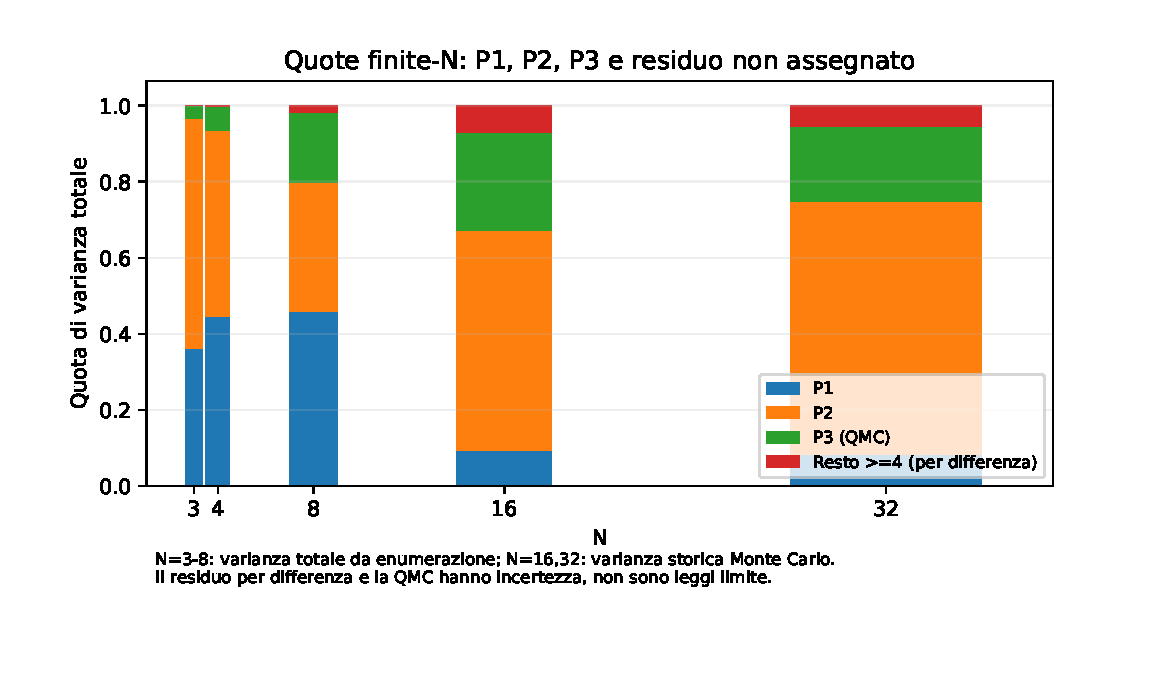
\includegraphics[width=0.83\linewidth]{r12ag_variance_fraction.pdf}
\caption{Scomposizione della varianza a dimensione finita. Il residuo non assegnato non puo essere estrapolato come nullo.}
\end{figure}
\begin{figure}[htbp]
\centering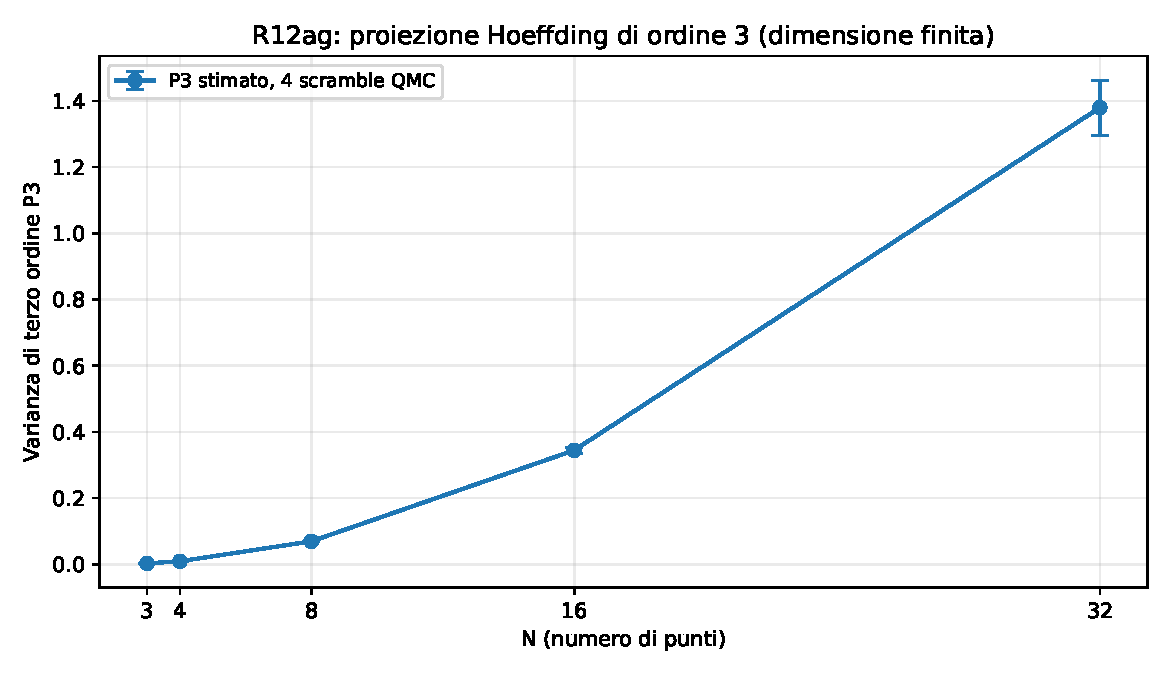
\includegraphics[width=0.81\linewidth]{r12ag_p3_uncertainty.pdf}
\caption{Stima del contributo di terzo ordine con incertezza tra quattro repliche QMC preregistrate.}
\end{figure}

\subsection{Il quarto ordine non e identicamente nullo}

Un test supplementare \emph{esatto, non annoverato tra i 31 controlli prospettici}, costruisce quattro coppie di posizioni razionali per $Z_1,\ldots,Z_4$ (coordinate riportate in \texttt{R12AG\_EXACT\_FOURTH\_WITNESS.json}) e calcola con frazioni esatte la differenza alternata sulle $2^4$ scelte. Ne risulta
\begin{equation}
 \sum_{b\in\{0,1\}^4}(-1)^{|b|}S_4(z_1^{b_1},z_2^{b_2},z_3^{b_3},z_4^{b_4})
 =\frac{583443}{6250000}\ne0.
 \label{eq:r12ag_D4}
\end{equation}
Qualunque funzione che sia somma di termini dipendenti da al piu tre dei quattro argomenti ha quarta differenza alternata identicamente nulla; dunque $h_{4,4}\not\equiv0$. Poiche le relazioni d'ordine dei punti restano invariate in intorni aperti delle coordinate scelte, tale differenza non nulla vale su un insieme di misura positiva: \textbf{$P_{4,4}>0$}. Questa e una dimostrazione \emph{per $N=4$}, non una prova di una quota non nulla al limite $N\to\infty$.

\subsection{Verdetto e vincolo sul ramo successivo}

R12ag ottiene una terza proiezione esatta a $N$ finito e conferma numericamente che $P_3$ spiega una parte sostanziale del residuo precedente nel range verificato. Una quarta proiezione non banale e provata a $N=4$, quindi il residuo non puo essere posto arbitrariamente a zero. \textbf{Non e stato derivato ne un ordine sharp di $\mathrm{Var}(S_N)$, ne un CLT/LDP, ne una stima uniforme del resto $V_{\ge4,N}$}. Lo stato e \nolinkurl{R12AG_THIRD_PROJECTION_EXACT_FINITE_N_VALIDATED_HIGHER_ORDER_SCALING_OPEN}. Il Gate R12ah dovra scegliere e preregistrare una via realmente asintotica (clustering delle covarianze, cancellazione controllata dei livelli alti, oppure un blocker dimostrato), non prolungare automaticamente fit finite-$N$. Il problema di fase a $g=1$, il path sum Lorentziano 4d e la chiusura cosmologica restano non risolti; \textbf{R13 resta BLOCCATO}.

\section{Gate R12ah: certificato di resampling del residuo Hoeffding e verifica strategica}
\label{sec:r12ah}

Il Gate R12ag ha dimostrato che i primi tre livelli Hoeffding non esauriscono, in generale, l'azione positiva 2d. Per evitare di costruire in sequenza infiniti kernel ad alto ordine, R12ah cerca un \emph{controllo dell'intera somma dei livelli superiori} valido a ogni dimensione finita $N$. Restano invariati l'ensemble di $N$ punti iid uniformi in $[0,1]^2$ e $\epsilon=0.21$. Nessuna misura Lorentziana e implicata.

\subsection{Una identita di resampling esatta in $N$}

Scriviamo la decomposizione canonica della funzione simmetrica $S_N=f_N(Z_1,\ldots,Z_N)$:
\begin{equation}
S_N-\mathbb E_0 S_N=\sum_{\varnothing\ne A\subseteq[N]} h_A(Z_A),\qquad
P_{r,N}=\sum_{|A|=r}\mathbb E_0[h_A^2]\ge0,\qquad
V_{\ge4,N}=\sum_{r=4}^N P_{r,N}.
\label{eq:r12ah_decomposition}
\end{equation}
Sia $0<p<1$. Costruiamo $Z_i^{(p)}$ mantenendo $Z_i$ con probabilita $p$ e sostituendolo altrimenti con una copia iid $\widetilde Z_i$, indipendentemente per ogni $i$; $S_N^{(p)}=f_N(Z_1^{(p)},\ldots,Z_N^{(p)})$. Tutte le marginali mantengono esattamente la distribuzione iniziale. Per degenerazione canonica dei nuclei Hoeffding,
\begin{equation}
 \mathbb E_0\bigl[h_A(Z_A^{(p)})\mid Z_1,\ldots,Z_N\bigr]=p^{|A|}h_A(Z_A).
 \label{eq:r12ah_operator}
\end{equation}
Infatti un termine condizionato sopravvive soltanto se \emph{tutti} gli indici di $A$ sono conservati: se un solo indice viene risamplato, l'integrazione di quel punto annulla il nucleo. Dall'ortogonalita esatta otteniamo
\begin{align}
 C_N(p)&\equiv\operatorname{Cov}_0(S_N,S_N^{(p)})=\sum_{r=1}^N p^r P_{r,N},\label{eq:r12ah_cov}\\
 D_N(p)&\equiv\tfrac12\mathbb E_0[(S_N-S_N^{(p)})^2]=\sum_{r=1}^N(1-p^r)P_{r,N}.\label{eq:r12ah_D}
\end{align}
\textbf{Teorema (certificato dell'intero residuo).} Per $N\ge4$, definendo
\begin{equation}
 B_N(p)\equiv D_N(p)-\sum_{r=1}^3(1-p^r)P_{r,N}
 =\sum_{r=4}^N(1-p^r)P_{r,N},
 \label{eq:r12ah_B}
\end{equation}
la positivita di ogni $P_{r,N}$ implica
\begin{equation}
 \boxed{(1-p^4)V_{\ge4,N}\le B_N(p)\le(1-p^N)V_{\ge4,N}}
 \quad\Longrightarrow\quad
 \boxed{\frac{B_N(p)}{1-p^N}\le V_{\ge4,N}\le\frac{B_N(p)}{1-p^4}}.
 \label{eq:r12ah_sandwich}
\end{equation}
Al valore \emph{preregistrato} $p=1/2$ segue il corollario semplice, uniforme in $N$,
\begin{equation}
 \boxed{B_N\le V_{\ge4,N}\le\tfrac{16}{15} B_N}.\label{eq:r12ah_half}
\end{equation}
Il fattore $16/15$ e ottimale per questo certificato universale: viene saturato nel caso di un caos puro di ordine quattro. La forma raffinata nella Eq.~\eqref{eq:r12ah_sandwich} tiene anche conto dell'ordine massimo finito $N$. \textbf{Le formule sono esatte soltanto per le aspettative vere}: sostituire un campione Monte Carlo a $B_N$ non produce automaticamente un limite statistico garantito.

\subsection{Controlli prospettici e diagnostica numerica}

Il protocollo \texttt{R12AH\_PREREGISTRATION.json} e stato congelato prima dei nuovi campioni (digest SHA-256 nel pacchetto). I 125 controlli deterministici e di confronto indipendente del calcolatore dell'azione sono tutti superati; la nuova produzione conserva $\epsilon=0.21$ e $p=1/2$ su quattro stream iid distinti per taglia. Nessun dato e stato scartato. Per $B_N$ sono impiegati i valori storici $P_1,P_2$ e $P_3$, con l'incertezza QMC di quest'ultimo esplicitata.

\begin{table}[htbp]
\centering\small
\caption{R12ah. Coppie indipendenti nel campionamento positivo 2d. Le incertezze riportate sono SE diagnostici, non intervalli di copertura garantita. $B$ e stimato con plug-in delle proiezioni pregresse.}
\label{tab:r12ah_samples}
\begin{tabular}{r r r r r}
\toprule
$N$ & coppie & $\widehat D_N\pm\mathrm{SE}$ & $\widehat B_N\pm\mathrm{SE}_{\mathrm{nota}}$ & $\widehat V_{\ge4}^{\mathrm{stor.}}$\\
\midrule
8 & 131072 & $0.25310\pm0.00116$ & $0.00877\pm0.00142$ & 0.00720\\
16 & 65536 & $0.99335\pm0.00592$ & $0.05508\pm0.00953$ & 0.09279\\
32 & 32768 & $5.26732\pm0.04265$ & $0.30947\pm0.08421$ & 0.37980\\
64 & 16384 & $19.10674\pm0.21498$ & n.d. & n.d.\\
\bottomrule
\end{tabular}
\end{table}

Le medie marginali dei nuovi stream sono coerenti, entro i cinque SE preregistrati, con $\mathbb E_0 S_N=4[1-(1-\epsilon)^N]$. Il SE indicato per $B$ combina il solo errore del nuovo $\widehat D$ e quello QMC noto di $P_3$, \emph{non} gli errori di $P_1,P_2$ o una copertura frequentista esatta. \textbf{Le vecchie stime puntuali del residuo per differenza, soprattutto a $N=16$, non rientrano nei nuovi intervalli plug-in puntuali}: entrambe le parti contengono errori di stima, inclusa la varianza totale storica basata su un campione diverso. La discordanza e conservata come limite dell'audit; non viene trasformata in una conferma né corretta scegliendo nuove soglie. Rimane non dimostrato il limite $V_{\ge4,N}/\operatorname{Var}_0(S_N)\to0$.

\begin{figure}[htbp]
\centering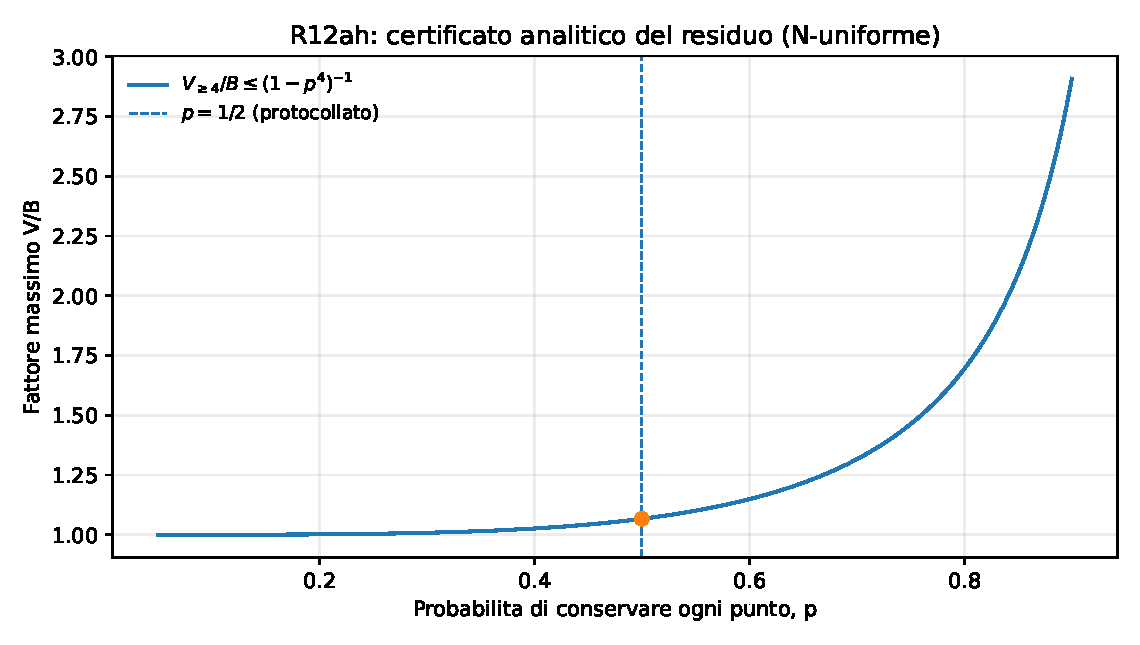
\includegraphics[width=0.80\linewidth]{r12ah_noise_bound.pdf}
\caption{Fattore esatto $1/(1-p^4)$ della disuguaglianza superiore sul residuo; a $p=1/2$ vale $16/15$. Non e una fascia di confidenza statistica.}
\end{figure}
\begin{figure}[htbp]
\centering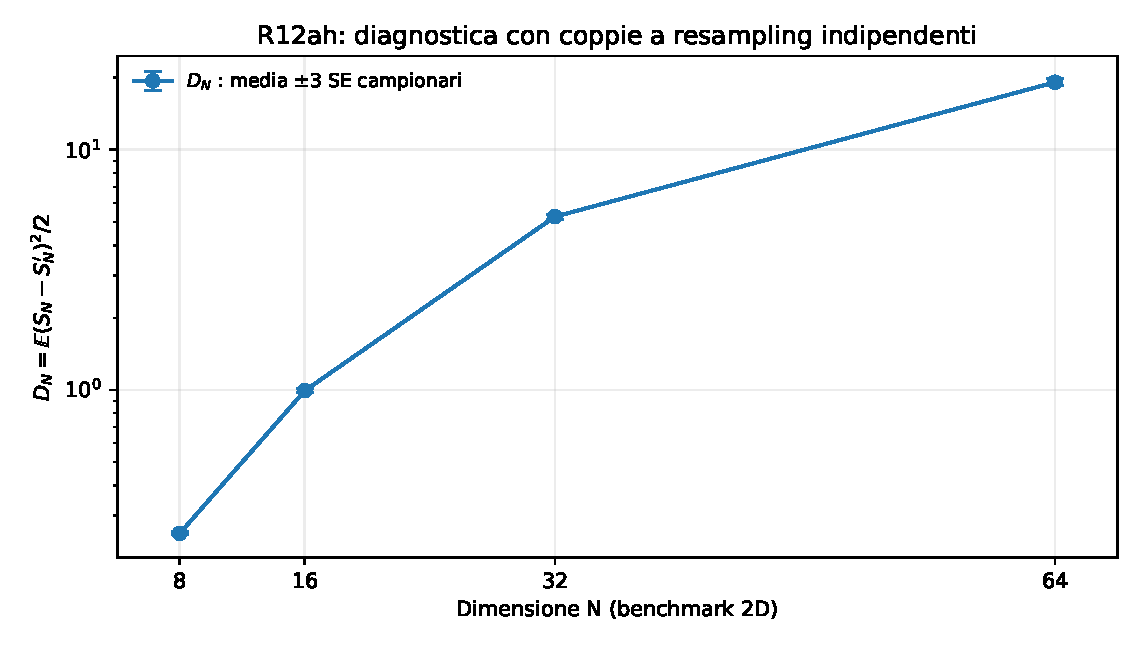
\includegraphics[width=0.80\linewidth]{r12ah_noise_data.pdf}
\caption{Diagnostica Monte Carlo del termine $D_N$ con tre errori standard campionari. Non inferire una potenza asintotica dalle quattro taglie.}
\end{figure}

\subsection{Perche la concentrazione normalizzata non prova la dominanza dei primi ordini}

Dal Gate R12ac si eredita il bound $\operatorname{Var}_0(S_N)=O_\epsilon(N(1+\log N)^2)$, dunque anche $V_{\ge4,N}/N^2\to0$. Ma questa conclusione non dimostra che il \emph{rapporto} del residuo con la varianza totale tenda a zero. Per un controesempio universale non BDG, con variabili Rademacher indipendenti $\xi_i=\pm1$, si consideri
\begin{equation}
 F_N=\sqrt{\frac{N}{\binom N4}}\sum_{i<j<k<\ell}\xi_i\xi_j\xi_k\xi_\ell.
 \label{eq:r12ah_fourth_chaos}
\end{equation}
Per ortogonalita esatta, $\operatorname{Var}(F_N)=N$ ed \emph{esclusivamente} $P_{4,N}=N$ e non nullo: pertanto $F_N/N\to0$ in $L^2$, pur essendo il residuo di quarto ordine pari al 100\% della varianza. Il controesempio vieta una deduzione automatica dalla sola concentrazione; non dimostra che la stessa situazione avvenga per l'azione causale.

\subsection{Verdetto e priorita del progetto}

R12ah fornisce una identita di resampling e un certificato uniforme per l'\emph{intero} resto ad ogni $N$ finito, con test riproducibili. Non fornisce un ordine sharp della varianza, un CLT/LDP, una stima asintotica relativa del residuo, o la funzione caratteristica a $g=1$. Una norma Hoeffding positiva in 2d non determina una sorgente gravitazionale Lorentziana 4d conservata. La classificazione e
\begin{center}
\small\nolinkurl{R12AH_EXACT_NOISE_TAIL_SANDWICH_FINITE_N_VALIDATED_ASYMPTOTIC_RELATIVE_TAIL_OPEN_2D_BRANCH_PAUSED}.
\end{center}
\textbf{Decisione di roadmap:} la prosecuzione automatica verso kernel $h_4,h_5,\ldots$ del benchmark 2d viene messa in pausa. Il nuovo Gate R12ai deve verificare i requisiti di un ponte fisico 4d (misura Lorentziana, noise tensor covariante conservato, Ward/Bianchi, scala mesosopica e limite continuo). Questa e una scelta metodologica, non un no-go generale. \textbf{R13 resta BLOCCATO}.\par


\section{Gate R12ai: audit del ponte fisico 4d e costruzione conservata su sfondo piatto}
\label{sec:r12ai}

Il punto di verifica R12ah ha sospeso l'estensione automatica delle proiezioni Hoeffding del \emph{benchmark positivo 2d}. Il nuovo problema e distinto: stabilire quali oggetti siano necessari per un \emph{path sum Lorentziano 4d} e una sorgente gravitazionale conservata. Il protocollo \texttt{R12AI\_PREREGISTRATION.json}, conservato con impronta SHA-256 prima delle nuove verifiche, separa un controllo costruttivo in Minkowski dalla dimostrazione di una dinamica fisica. Non si seleziona una funzione $H(t)$, una $\Lambda(t)$ o un accoppiamento per ottenere accelerazione.

\subsection{Oggetti del controllo e condizione di conservazione}

La costruzione R12g definiva, dati gli insiemi dei passati causali troncati $P_x$, un campo scalare casuale cumulativo. Formalizziamolo in uno spazio-tempo piatto di dimensione quattro, con volume $V_x=V_4(P_x)>0$, rumore centrato indipendente sul quattro-volume $W$ e ampiezza $A$ non selezionata:
\begin{equation}
 \phi(x)=\frac{A}{V_x}\int_{P_x}\!dW(u),\qquad
 K(x,y)=\mathbb E[\phi(x)\phi(y)]
 =A^2\frac{V_4(P_x\cap P_y)}{V_xV_y}.
 \label{eq:r12ai_overlap_K}
\end{equation}
Questa definizione e una \emph{idealizzazione stocastica classica} su uno sfondo assegnato; l'integrale e inteso come integrale rispetto a un rumore indipendentemente distribuito, non come una misura quantistica dei causal set. Il troncamento $t\ge0$ e una condizione al bordo che fissa una foliazione; non viene rivendicata invarianta globale sotto i boost del vuoto. La correlazione normalizzata e $V_4(P_x\cap P_y)/\sqrt{V_xV_y}$. Per qualunque insieme finito di coefficienti reali $c_i$,
\begin{equation}
 \sum_{i,j}c_ic_jK(x_i,x_j)
 =A^2\int dV_u\left[\sum_i\frac{c_i\,\mathbf1_{P_{x_i}}(u)}{V_{x_i}}\right]^2\!\ge0.
 \label{eq:r12ai_psd_overlap}
\end{equation}
La positivit\`a e quindi un risultato di Gram esatto, valido anche per osservazioni spazialmente diverse, non un fit. Il kernel grezzo ha tuttavia la cuspide gia identificata in R12h; le derivate che seguono devono essere interpretate \emph{come distribuzioni} su funzioni di prova, oppure dopo uno smearing esplicitamente dichiarato.

\subsection{Un tensore conservato in Minkowski: risultato costruttivo limitato}

Nella metrica $\eta_{\mu\nu}=\mathrm{diag}(-1,1,1,1)$ poniamo
\begin{equation}
 \Xi_{\mu\nu}=D_{\mu\nu}\phi,
 \qquad D_{\mu\nu}:=\partial_\mu\partial_\nu-\eta_{\mu\nu}\Box,
 \qquad\Box=\eta^{\rho\sigma}\partial_\rho\partial_\sigma.
 \label{eq:r12ai_flat_projector}
\end{equation}
Poiche le derivate ordinarie commutano, \emph{distribuzionalmente},
\begin{equation}
 \boxed{\partial^\mu\Xi_{\mu\nu}=(\Box\partial_\nu-\partial_\nu\Box)\phi=0.}
 \label{eq:r12ai_flat_ward}
\end{equation}
Il corrispondente kernel tensoriale $\mathcal N_{\mu\nu\rho\sigma}(x,y)
 =D^x_{\mu\nu}D^y_{\rho\sigma}K(x,y)$ e trasverso in entrambi gli argomenti. Per funzioni di prova tensoriali reali $f^{\mu\nu}$ a supporto compatto,
\begin{equation}
 \mathcal N(f,f)=\mathbb E\!\left[\left(\int d^4x\,f^{\mu\nu}(x)\Xi_{\mu\nu}(x)\right)^2\right]\ge0,
 \label{eq:r12ai_tensor_psd}
\end{equation}
perche e la covarianza di una trasformazione lineare del campo scalare. Si e dunque ottenuto un \emph{esempio} di rumore tensoriale positivo e conservato sullo sfondo piatto, \textbf{non} un teorema di unicita ne il noise kernel quantistico di un operatore energia--impulso. In particolare la costruzione occupa un settore di tipo scalare: non determina l'ampiezza, gli eventuali contributi spin--2 indipendenti, la risposta dissipativa ne una misura oscillante $e^{iS_{4d}}$. Il precedente fisico che integra un vero stress quantistico, il suo noise kernel e la risposta e la stochastic gravity \cite{HuVerdaguer2008}.

Un controllo molto concreto mostra perche la conservazione formale non risolve la cosmologia. Per $\phi=f(t)$ omogeneo su Minkowski,
\begin{equation}
 \Xi_{00}=0,\qquad \Xi_{0i}=0,\qquad\Xi_{ij}=\delta_{ij}\,\ddot f(t).
 \label{eq:r12ai_hom_flat}
\end{equation}
Quindi questo esempio non genera nemmeno una densita energetica omogenea di vuoto sullo sfondo piatto: costruire un tensore trasverso non equivale a produrre la componente cosmologica cercata.

\subsection{Ostacolo in FLRW: la conservazione non sopravvive alla covariantizzazione ingenua}

Sostituire semplicemente $\partial$ con $\nabla$ nell'operatore di Eq.~\eqref{eq:r12ai_flat_projector} non preserva l'identita: per uno scalare $F$, $\nabla^\mu(\nabla_\mu\nabla_\nu-g_{\mu\nu}\Box)F=R_{\nu\sigma}\nabla^\sigma F$. Una possibilita strutturalmente piu motivata emerge variando metricamente il termine $\int\!d^4x\sqrt{-g}\,F R$. Il tensore associato, con convenzione qui adottata, e
\begin{equation}
 \mathcal A_{\mu\nu}[g,F]=F G_{\mu\nu}+
 (g_{\mu\nu}\Box-\nabla_\mu\nabla_\nu)F.
 \label{eq:r12ai_covariant_attempt}
\end{equation}
Da Bianchi e dal commutatore di derivate segue esattamente
\begin{equation}
 \boxed{\nabla^\mu\mathcal A_{\mu\nu}=-\frac12 R\nabla_\nu F.}
 \label{eq:r12ai_noether_obstruction}
\end{equation}
Per un $F$ \emph{esterno casuale} e una metrica curva generica, il membro destro non si annulla: la diffeomorphism invariance dell'espressione scritta usando un campo esterno non garantisce da sola una sorgente conservata. Se $F$ e un grado di liberta dinamico, la sua equazione di moto e gli eventuali contributi addizionali allo stress possono restaurare la identita di Ward \emph{on-shell}; l'azione e la sua dinamica devono pero essere effettivamente specificate.

Per verificare il segno e l'ordine del residuo, in FLRW piatto in unita $c=1$, con $H=\dot a/a$ e $F=F(t)$, le componenti effettive dell'Eq.~\eqref{eq:r12ai_covariant_attempt} sono
\begin{align}
 \rho_{\mathcal A}=\mathcal A_{00}&=3H^2F+3H\dot F,\\
 p_{\mathcal A}=\mathcal A_{ii}/a^2&=-(2\dot H+3H^2)F-\ddot F-2H\dot F,
\end{align}
e verificano
\begin{equation}
 \dot\rho_{\mathcal A}+3H(\rho_{\mathcal A}+p_{\mathcal A})
 =\frac{R}{2}\dot F,\qquad R=6(\dot H+2H^2).
 \label{eq:r12ai_flrw_balance}
\end{equation}
Con $a\propto t^{2/3}$ (materia) e la scelta diagnostica $F=t^2$, si ha $R=4/(3t^2)$ e $\nabla^\mu\mathcal A_{\mu0}=-4/(3t)\ne0$. Questa e una verifica \emph{contro} la pretesa di conservazione automatica, non un nuovo modello di materia o un fit cosmologico.

\subsection{Audit esplicito dei requisiti 4d}

L'azione BDG e un oggetto noto in dimensione quattro, ma con coefficienti \emph{dipendenti dalla dimensione}; nella convenzione degli intervalli aperti $N_j$ la sua struttura non-smeared contiene $N-N_0+9N_1-16N_2+8N_3$ (a fattori dimensionali dipendenti da $\ell/\ell_p$), diversamente dall'azione regolarizzata del nostro benchmark 2d \cite{BenincasaDowker2010,Carlip2024}. Anche scrivere formalmente $Z_N=\sum_{C\in\Omega_N}\mu(C)e^{iS^{(4)}_{\rm BDG}[C]}$ non definisce \emph{da solo} la misura fisica: servono la classe $\Omega_N$, i pesi, la gestione delle simmetrie, il bordo, la prescrizione di limite, l'operatore di sorgente e il suo accoppiamento con la geometria. La soppressione di classi non-manifold-like riportata in letteratura non implica che sia gia derivato il settore fisico residuo \cite{Carlip2024}.

\begin{center}
\small
\begin{tabular}{p{0.38\linewidth}p{0.18\linewidth}p{0.34\linewidth}}
\toprule
\textbf{Requisito} & \textbf{Esito} & \textbf{Limite}\tabularnewline\midrule
Overlapping past in Minkowski 4d, $K\succeq0$ & \status{PASS TOY} & Geometria piu rumore classico assunto.\\
$\partial^\mu\Xi_{\mu\nu}=0$, $\mathcal N\succeq0$ & \status{PASS PIATTO} & Identita distribuzionale, non microdinamica.\\
Sorgente curva conservata \emph{on-shell} & \status{NON DERIVATA} & Il campo esterno lascia $-R\,dF/2$.\\
Noise tensor completo + risposta causale & \status{NON SELEZ.} & Amplitudine, spin--2, dissipazione liberi.\\
Misura Lorentziana 4d regolata e normalizzata & \status{NON SPECIFIC.} & Ensemble, pesi, bordo e convergenza mancanti.\\
Continuum/mesoscale e matching alle sorgenti & \status{NON DERIV.} & Non trasferire risultati 2d.\\
Chiusura cosmologica e predizioni R13 & \status{BLOCCATO} & Nessun $H(z)$ indipendente.\\
\bottomrule
\end{tabular}
\end{center}

Il controllo diagnostico preregistrato usa $16$ eventi nel Minkowski 4d e $10^4$ celle di rumore uniforme; la matrice normalizzata dei passati ha autovalore minimo $\simeq0.07746$. Una trasformazione lineare mantiene la covarianza semidefinita positiva (il minimo numerico $-4.9\times10^{-14}$ deriva dall'arrotondamento). Sono passate inoltre le verifiche simboliche della Ward identity piatta, della traccia, del settore omogeneo e dell'ostruzione FLRW. Questi sono \emph{test di implementazione} di risultati algebrici, non validazione empirica della gravita quantistica.

\begin{figure}[H]
\centering
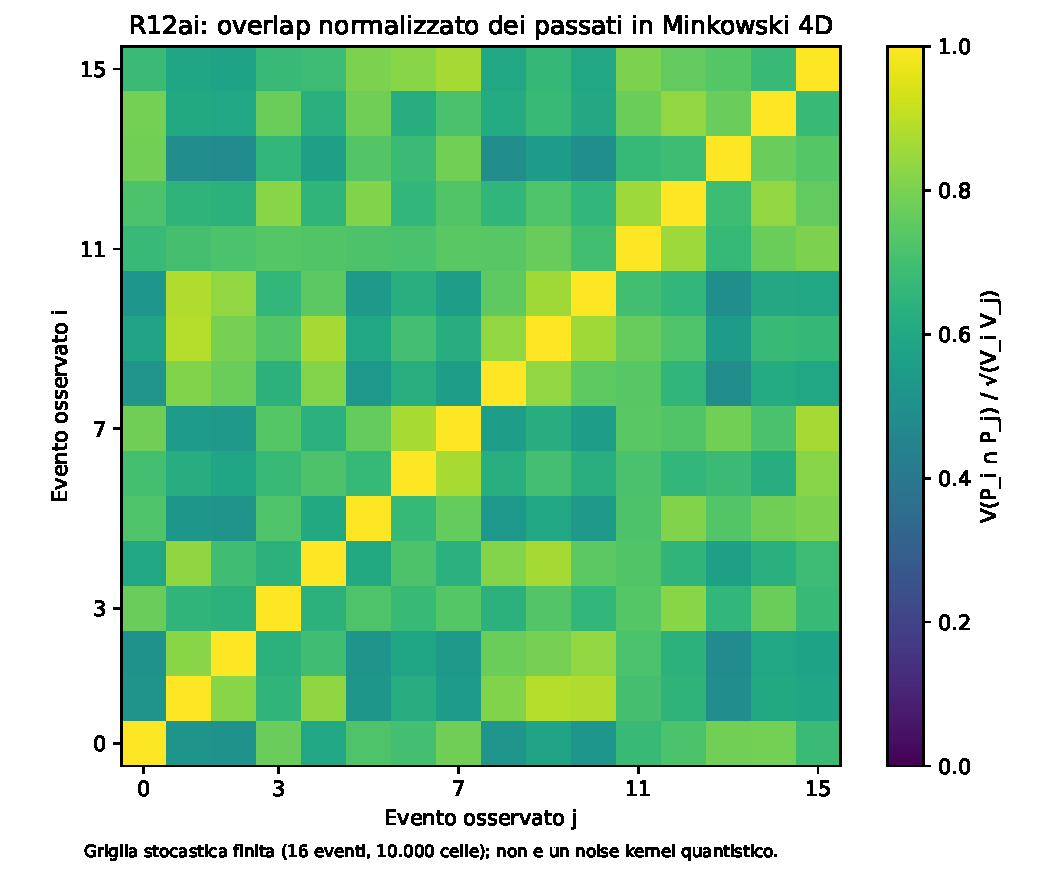
\includegraphics[width=0.66\linewidth]{r12ai_overlap_gram.pdf}
\caption{R12ai, controllo diagnostico del kernel scalare di overlap in Minkowski 4d: correlazioni normalizzate di 16 eventi, valutate su 10.000 celle di volume. La semidefinita positivita vale per la costruzione di Gram, indipendentemente dalla dimensione della griglia; la figura non rappresenta un noise kernel quantistico.}\label{fig:r12ai_overlap_gram}
\end{figure}

\subsection{Verdetto R12ai e passo successivo}

\begin{center}
\small\nolinkurl{R12AI_FLAT_WARD_PSD_CONSTRUCTION_PASS_CURVED_4D_MICRODYNAMICS_NOT_DERIVED_R13_BLOCKED}
\end{center}

\textbf{Contributo effettivo:} l'overlap scalare ammette un'esplicita \emph{tensorizzazione conservata e positiva} \emph{in Minkowski} a livello di distribuzioni, senza assumere una forma arbitraria del noise kernel. Questo non contraddice il no-go ristretto R12i sulla \emph{selezione unica} del noise tensor fisico: la costruzione sceglie un particolare operatore $D_{\mu\nu}$ che non e selezionato dall'overlap stesso. L'ostruzione curva rende esplicito il costo della scelta. \textbf{Verdetto fisico:} mancano una microdinamica 4d, una misura Lorentziana controllata, un'origine dinamica on-shell della sorgente, il settore di risposta e il limite continuo; percio \textbf{R13 resta BLOCCATO}. Il prossimo Gate R12aj verra delimitato alla \emph{specificazione di un singolo candidato 4d action-plus-measure con identita di Ward e operatore di sorgente} e ai suoi controlli minimi; nessun valore di $\Lambda$ o $H(t)$ va introdotto per rendere il candidato accelerante.

\section{Gate R12aj: misura oscillante BDG in 4d, definizione finita e blocco della sorgente}
\label{sec:r12aj}

\textbf{Domanda del gate.} Dopo il controllo R12ai, il problema non e piu costruire un altro tensore formalmente trasverso: occorre stabilire se un singolo candidato \emph{azione piu misura} in quattro dimensioni determini anche una sorgente gravitazionale generalmente covariante e la sua risposta causale. Il protocollo \texttt{R12AJ\_PREREGISTRATION.json} e stato fissato e registrato con SHA-256 prima dei test prospettici. Per isolare i requisiti, si prende il candidato piu vicino alla microstruttura gia discussa: l'azione BDG standard in quattro dimensioni e uno sprinkling a numero fissato su Minkowski. \textbf{Il modello cosi definito e un test di fattibilita cinematica e non viene identificato con il path sum quantistico 4d completo.}

\subsection{Un solo candidato esplicito: ensemble condizionato e fase BDG}

Sia $\mathcal D=J^+(p)\cap J^-(q)\subset\mathbb M^{1,3}$ un diamante di Minkowski con $p=(-1,\mathbf 0)$ e $q=(+1,\mathbf 0)$, in unita $c=1$. Esplicitamente $\mathcal D=\{(t,\mathbf x):|t|+\|\mathbf x\|<1\}$, di quattro-volume $V_{\mathcal D}=2\pi/3$. Per $N$ fissato, campioniamo $X=(x_1,\ldots,x_N)$ indipendentemente dalla misura di volume \emph{positiva} normalizzata
\begin{equation}
 dP_{0,N}(X)=\prod_{i=1}^{N}\frac{d^4x_i}{V_{\mathcal D}},
 \qquad C(X):\quad i\prec j\iff x_j\in J^+(x_i),
 \label{eq:r12aj_sprinkling}
\end{equation}
con causalita stretta e trascurando separazioni esattamente nulle, di probabilita zero. E' la distribuzione condizionata sul numero di eventi di uno sprinkling Poisson sullo sfondo fissato. Il numero $N$ non e una variabile dinamica del modello di test e il diamante e una condizione al bordo \emph{imposta}.

Per una coppia ordinata causalmente $i\prec j$, l'intervallo aperto contiene $|I(i,j)|=|\{k:i\prec k\prec j\}|$ elementi. Sia $N_k(C)$ il numero di tali coppie per cui $|I(i,j)|=k$. L'azione \emph{non smeared} BDG in quattro dimensioni e, nella convenzione standard \cite{BenincasaDowker2010,Surya2019Review},
\begin{equation}
 \frac{S^{(4)}_{\rm BDG}(C)}{\hbar}
 =\frac{4}{\sqrt 6}\left(\frac{\ell}{\ell_P}\right)^2
 \bigl(N-N_0+9N_1-16N_2+8N_3\bigr).
 \label{eq:r12aj_action4}
\end{equation}
Il prefattore contiene la lunghezza di discrezione $\ell$ e la scala planckiana $\ell_P$; \textbf{porre $\ell/\ell_P=1$ e $g=1$ nei soli test numerici e una convenzione diagnostica, non una predizione della teoria e non una prescrizione fisica del limite continuo}. Il parametro $\epsilon=0.21$ del vecchio benchmark 2d non viene riutilizzato in modo improprio in questa azione 4d. La funzione caratteristica finita e
\begin{equation}
 \Phi_N(g)=\int_{\mathcal D^N}dP_{0,N}(X)\,
 \exp\!\left[ig\,\frac{S^{(4)}_{\rm BDG}(C(X))}{\hbar}\right],
 \qquad |\Phi_N(g)|\le1.
 \label{eq:r12aj_phi4}
\end{equation}
L'integrale e \emph{matematicamente ben definito per ogni $N$ finito}: la misura positiva e una probabilita e la fase ha modulo uno. Si tratta pero di un \emph{reweighting oscillante di sprinklings su un background assegnato}, non di una misura quantistica ottenuta sommando geometricamente tutti i causal set 4d con i loro pesi fisici e le loro condizioni di bordo. Scegliere soltanto causal set che si immergono nel diamante e gia una restrizione forte della classe di storie; la probabilita $P_{0,N}$ e un input esterno, non deriva dall'azione.

\subsection{Benchmark esatto a due eventi e protocollo finito}

La frazione di coppie confrontabili in un diamante Alexandrov uniforme in dimensione $d$ soddisfa la formula di Myrheim--Meyer \cite{Surya2019Review}
\begin{equation}
 p_d=\frac{\Gamma(d+1)\Gamma(d/2)}{2\Gamma(3d/2)},
 \qquad p_4=\frac1{10}.
 \label{eq:r12aj_comparable}
\end{equation}
Per $N=2$ esistono due possibilita: coppia comparabile, $N_0=1$ e $S_4/\hbar=a$; coppia incomparabile, $N_0=0$ e $S_4/\hbar=2a$, con $a=4/\sqrt6$ e $\ell/\ell_P=1$. Da qui segue la verifica analitica senza fit
\begin{equation}
 \boxed{\Phi_2(g)=\tfrac9{10}e^{2iga}+\tfrac1{10}e^{iga}.}
 \label{eq:r12aj_phi2}
\end{equation}
Il programma indipendente \texttt{r12aj\_sprinkling\_audit.py} estrae punti uniformi in quattro-volume, costruisce l'ordine causale e verifica due metodi di conteggio degli intervalli. Prima della produzione sono stati congelati semi, taglie $N=2,8,16,32,64$, numerosita $M=32768,4096,4096,2048,1024$ e soglie dei confronti per $N=2$. Per ogni taglia si controllano inoltre transivit\`a, assenza di cicli, rietichettatura e invarianti sotto un boost applicato a \emph{eventi e diamante insieme}. Quest'ultimo controllo e una simmetria globale di Minkowski, \emph{non} una Ward identity locale della gravita.

Per la media complessa $\widehat\Phi_N$ di $M$ fasi indipendenti, una disuguaglianza di Hoeffding sulle parti reale e immaginaria da, senza assumere gaussianita,
\begin{equation}
 \Pr\!\left(\left|\widehat\Phi_N-\Phi_N\right|\le r_{99}(M)\right)\ge0.99,
 \quad r_{99}(M)=\sqrt{\frac{4\ln 400}{M}},
 \label{eq:r12aj_hoeffding}
\end{equation}
\emph{per ciascuna taglia considerata separatamente}. Dichiariamo ``fase risolta rispetto a zero'' solo quando il disco di confidenza non contiene l'origine, cioe $|\widehat\Phi_N|>r_{99}$. Non si impone una legge asintotica alle taglie non risolte.

\begin{table}[htbp]
 \centering\small
 \caption{Gate R12aj: test oscillante a $g=1$, con prefattore diagnostico $\ell/\ell_P=1$. La colonna $r_{99}$ e una soglia rigorosa per la media campionaria, non un errore sulla fisica cosmologica.}
 \label{tab:r12aj_phi}
 \begin{tabular}{rrrrll}
 \toprule
 $N$ & $M$ & $\widehat p_{\rm comp}$ & $|\widehat\Phi_N|$ & $r_{99}$ & Fase risolta \\
 \midrule
 2 & 32768 & 0.09903 & 0.90026 & 0.02704 & si\\
 8 & 4096 & 0.09939 & 0.11880 & 0.07649 & si\\
 16 & 4096 & 0.09953 & 0.01832 & 0.07649 & no\\
 32 & 2048 & 0.10068 & 0.02141 & 0.10818 & no\\
 64 & 1024 & 0.10027 & 0.03619 & 0.15298 & no\\
 \bottomrule
 \end{tabular}
\end{table}

I controlli prospettici preregistrati terminano con \textbf{1693/1693 PASS}. I dati grezzi, il codice e il risultato JSON fanno parte del recovery; l'uso della relazione analitica \eqref{eq:r12aj_phi2} elimina l'ambiguita del primo benchmark. L'assenza di risoluzione statistica per $N\ge16$ non significa $\Phi_N=0$: rappresenta soltanto il limite della statistica effettuata nel presente test. Non fornisce alcuna soluzione del \emph{sign problem}, e non eredita alcun esponente dal benchmark 2d.

\begin{figure}[htbp]
 \centering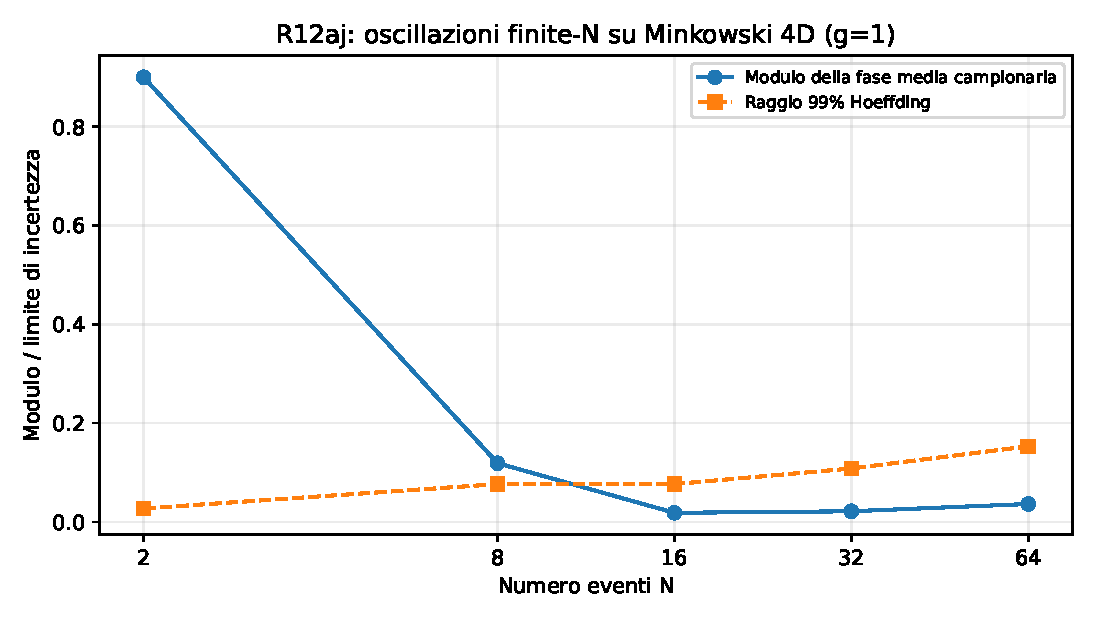
\includegraphics[width=0.80\linewidth]{r12aj_phase_resolution.pdf}
 \caption{Funzione caratteristica osc\-illante nell'ensemble di sprinkling 4d a sfondo fisso. Ogni punto rappresenta un campionamento indipendente e il limite superiore riportato e il raggio $r_{99}$ di Eq.~\eqref{eq:r12aj_hoeffding}; non e una curva di scaling fisico.}
 \label{fig:r12aj_phase_resolution}
\end{figure}

\begin{figure}[htbp]
 \centering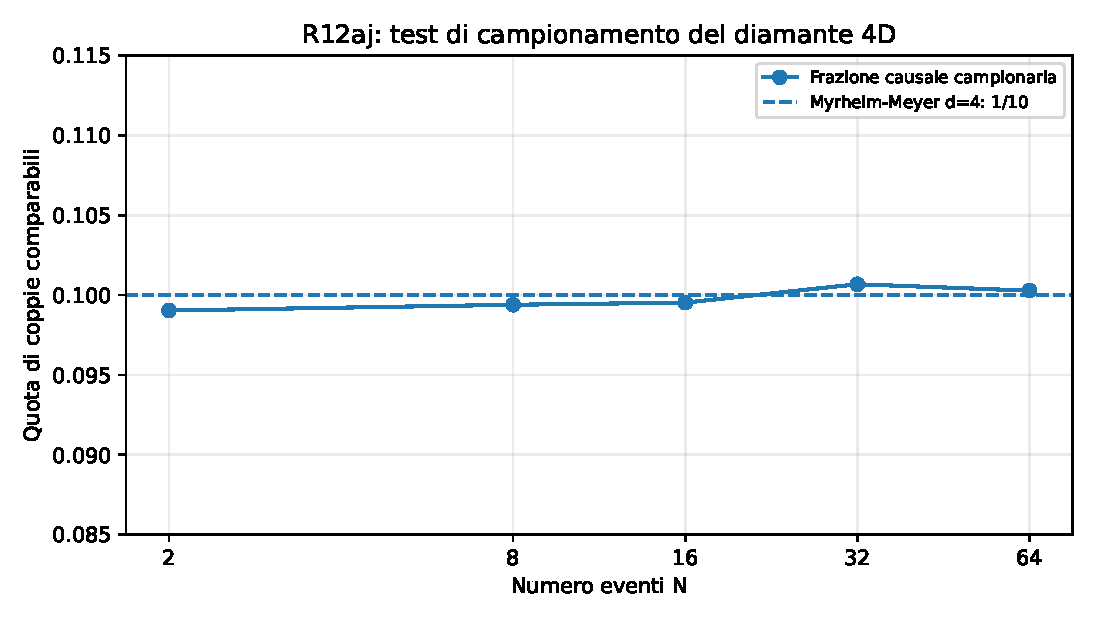
\includegraphics[width=0.80\linewidth]{r12aj_order_fraction.pdf}
 \caption{Frazione media delle coppie in relazione causale nel diamante piatto 4d e benchmark esatto $p_4=1/10$. E' un controllo del campionamento, non della dinamica.}
 \label{fig:r12aj_order_fraction}
\end{figure}

\subsection{Audit fisico: l'assenza di un operatore di sorgente e di una Ward dinamica}

La definizione \eqref{eq:r12aj_phi4} fornisce una fase oscillante a $N$ finito \emph{su} $(\mathcal D,\eta)$, ma \textbf{non fornisce un funzionale efficace $Z[g]$ per metriche dinamiche arbitrarie}. Di conseguenza \emph{non e definito dal candidato} un operatore energia--impulso della forma
\begin{equation}
 T_{\mu\nu}(x)\stackrel{?}{=}\frac{2}{\sqrt{-g}}\frac{\delta\Gamma[g]}{\delta g^{\mu\nu}(x)},
 \qquad\nabla^\mu T_{\mu\nu}=0\;\text{(on shell)},
 \label{eq:r12aj_missing_stress}
\end{equation}
né una sua versione puramente combinatoria con Ward equivalente. Non e lecito dichiarare il secondo membro nullo se il primo membro non e stato costruito. La reparametrizzazione delle etichette $i\mapsto\pi(i)$ e l'invarianza per boost dei dati \emph{non implicano} un'identita di Noether per variazioni arbitrarie di una metrica dinamica. A livello di una singola configurazione di punti a coordinate fissate, la sola relazione d'ordine e invariata sotto una trasformazione conforme $g_{\mu\nu}\mapsto\Omega^2(x)g_{\mu\nu}$: il numero di elementi e i conteggi di intervalli restano identici. Cio mostra quali informazioni metriche non sono contenute in quella \emph{variazione a campione fissato}; non e un no-go per una teoria causal-set completa, dove numero degli elementi, densita, misura e limiti possono codificare la scala fisica.

Il controllo va esteso a tre requisiti distinti. Primo, la sola azione $S_4(C)$ non sceglie una misura fisica sui \emph{causal set non etichettati}: $P_{0,N}$ seleziona un ensemble di immagini di immersioni nella geometria fissata e assegna loro probabilita secondo quel background. Secondo, manca una struttura \emph{closed-time-path} o equivalente che costruisca insieme un noise kernel quantistico e una \emph{risposta retarded}; una funzione caratteristica di un'azione scalare non e una funzione di risposta causale di uno stress quantistico \cite{HuVerdaguer2008}. Terzo, ne la scala di smearing $\ell_k>\ell$, ne il running con $\ell/\ell_P$, ne le condizioni al bordo gravitazionali necessarie a un limite continuo sono determinate. Il limite medio noto di BDG verso Einstein--Hilbert \cite{BenincasaDowker2010,Surya2019Review,MachetWang2021} non puo essere sostituito a una prova della convergenza del \emph{path sum oscillante} o a una derivazione del secondo cumulante fisico.

\begin{center}
\small
\begin{tabular}{p{0.42\linewidth}p{0.18\linewidth}p{0.31\linewidth}}
\toprule
\textbf{Requisito} & \textbf{Stato} & \textbf{Perche}\tabularnewline\midrule
Campione 4d e integralizzazione oscillante a $N$ finito & \status{PASS TOY} & $\mathcal D$, $P_{0,N}$, $S_4$ espliciti.\\
Order invariance / boost del dominio & \status{PASS TEST} & Simmetria di sfondo, non Ward gravitazionale.\\
Verifica analitica $N=2$ & \status{PASS} & Formula esatta di Eq.~\eqref{eq:r12aj_phi2}.\\
Misura quantistica su tutte le geometrie causali 4d & \status{NON DERIVATA} & La misura e background-conditioned.\\
Sorgente metrica on-shell / Ward--Bianchi & \status{ASSENTE} & $Z[g]$ e $T_{\mu\nu}$ non definiti.\\
Noise e risposta retarded & \status{ASSENTI} & Nessuna dinamica CTP o correlatore di stress.\\
Mesoscala, bordo e limite continuo & \status{APERTI} & $\ell/\ell_P=1$ e solo diagnostico.\\
Predizione autonoma $H(t)$ / R13 & \status{BLOCCATO} & Nessuna chiusura gravitazionale.\\
\bottomrule
\end{tabular}
\end{center}

\subsection{Verdetto R12aj e decisione fail-closed}

Il Gate R12aj supera \emph{solo} la specificazione di un \textbf{modello oscillante kinematico 4d a sfondo fissato}: l'azione BDG e il campionamento sono concreti e i controlli interni passano. \textbf{Non sopravvive al criterio di microdinamica gravitazionale completa}, poiche l'operatore di sorgente, la Ward on-shell, la misura su geometrie dinamiche, la risposta retarded e il limite continuo non sono derivati. Questa classificazione non smentisce la causal set theory: limita il candidato testato, che importa esplicitamente Minkowski nella misura. La classificazione congelata e
\begin{center}\small
\nolinkurl{R12AJ_FIXED_BACKGROUND_4D_BDG_AMPLITUDE_PASS_METRIC_WARD_SOURCE_RESPONSE_CONTINUUM_NOT_DERIVED_R13_BLOCKED}.
\end{center}
Il passo successivo non e aumentare ancora $N$ nel benchmark a sfondo fisso, ne forzare un fit di fase. Un eventuale R12ak deve \emph{prima} giustificare indipendentemente una nuova misura o un completamento variazionale dinamico con stato, bordo e sorgente conservata, e solo dopo autorizzare nuovi test. Se tale oggetto non viene selezionato senza assunzioni esterne arbitrarie, il ramo 4d termina come \emph{physical-closure blocker}. Le identita cinematiche $c+c$ restano vere ma non si trasformano in una nuova legge cosmologica. \textbf{R13 rimane BLOCCATO}.


\section{Gate R12ak: selezione della misura e decisione sul completamento fisico}
\label{sec:r12ak}

\textbf{Domanda e protocollo.} Il Gate R12aj definisce una funzione caratteristica per gli sprinklings su un diamante di Minkowski, ma non una somma dinamica su causal set fisici. R12ak e un \emph{gate condizionale}: prima di aggiungere altra dinamica, verifichiamo se il solo ordine causale, l'invarianza per rietichettatura e l'azione BDG 4d selezionino una misura univoca. Il protocollo \texttt{R12AK\_PREREGISTRATION.json} (SHA-256 congelato prima dell'enumerazione) fissa $N=1,\ldots,5$ e $g=1$, senza fit. Un controesempio in questa classe e sufficiente per un \emph{no-go ristretto sulla selezione da sola invarianza}, ma non per escludere altre microdinamiche.

\subsection{Due misure finite invarianti sullo stesso insieme di ordini}

Sia $\mathcal P_N^{\rm lab}$ l'insieme degli ordini parziali stretti su $N$ elementi distinguibili, e sia $\mathcal P_N^{\rm iso}$ il quoziente per isomorfismo. Denotiamo con $L_N$ e $U_N$ i rispettivi numeri di elementi. Per una classe $[C]$ e il suo gruppo di automorfismi, il teorema orbita--stabilizzatore fornisce
\begin{equation}
 m_N([C])=\frac{N!}{|\operatorname{Aut}(C)|}.
 \label{eq:r12ak_orbit}
\end{equation}
Due assegnazioni positive di \emph{peso di riferimento} sono entrambe invarianti rispetto a qualunque rietichettatura, ma non sono equivalenti:
\begin{equation}
 P_N^{\rm lab}([C])=\frac{m_N([C])}{L_N},\qquad
 P_N^{\rm iso}([C])=\frac1{U_N}.
 \label{eq:r12ak_measures}
\end{equation}
La prima nasce dal peso uniforme sui poset etichettati; la seconda dal peso uniforme sulle classi di isomorfismo. Non chiamiamo nessuna delle due ``misura quantistica fisica''; la scelta delle loro probabilita di riferimento e precisamente il problema in esame. La differenza e compatibile con la discussione gia presente nella letteratura causal-set sulla misura e sugli automorfismi \cite{Surya2019Review}.

Manteniamo \emph{esattamente} l'azione BDG diagnostica di R12aj, con intervalli \emph{aperti}, $\ell/\ell_P=1$ e $a_{\rm BDG}=4/\sqrt6$:
\begin{align}
 B_N(C)&=N-N_0(C)+9N_1(C)-16N_2(C)+8N_3(C),\\
 \Phi_N^{j}(g)&=\sum_{[C]\in\mathcal P_N^{\rm iso}}P_N^{j}([C])
 e^{i g a_{\rm BDG}B_N(C)},\qquad j\in\{\mathrm{lab},\mathrm{iso}\}.
 \label{eq:r12ak_amps}
\end{align}
Il parametro $4$ nei coefficienti BDG indica il \emph{benchmark di azione 4d}; \textbf{non vincola lo spazio di tutti i poset a causal set approssimabili da uno spazio-tempo quadridimensionale}. Questo e dunque un test esatto sulla liberta della \emph{misura}, non un path sum fisico 4d e non una sostituzione dell'ensemble di R12aj.

\subsection{Controesempio analitico a $N=2$}

Esistono due classi di isomorfismo: catena e anticatena. La prima ammette due ordini etichettati, la seconda uno. Per la catena $B_2=1$; per l'anticatena $B_2=2$. Quindi
\begin{align}
 \Phi_2^{\rm lab}(g)&=\frac23e^{iga_{\rm BDG}}+\frac13e^{2iga_{\rm BDG}},\\
 \Phi_2^{\rm iso}(g)&=\frac12e^{iga_{\rm BDG}}+\frac12e^{2iga_{\rm BDG}},\\
 \left|\Phi_2^{\rm lab}(g)-\Phi_2^{\rm iso}(g)\right|&=\frac{\left|\sin(ga_{\rm BDG}/2)\right|}{3}.
 \label{eq:r12ak_n2}
\end{align}
Al coupling storico diagnostico $g=1$ il modulo della differenza e $0.242917080270\ldots$, senza stima statistica. La probabilita di coppia comparabile dello sprinkling geometrico di R12aj e invece $1/10$ in un diamante Minkowski 4d, diversa sia da $2/3$ sia da $1/2$: \emph{tre leggi di riferimento diverse nonostante l'azione a due eventi sia la stessa}. Lo sprinkling resta un modello a \emph{background fissato}, non una terza misura quantistica selezionata.

\subsection{Enumerazione esaustiva, $N\le5$, e test indipendenti}

L'algoritmo genera tutti i tre stati possibili per ogni coppia non ordinata (prima $i\prec j$, poi $j\prec i$, oppure incomparabile), scarta le relazioni non transitive, calcola classi di isomorfismo e orbite di rietichettatura, e ricava la distribuzione \emph{esatta come frazioni razionali} del bracket $B_N$. Per $N\le4$ un secondo programma usa una verifica distinta della transitivita e del conteggio degli intervalli. I totali coincidono con le sequenze enumerative note \cite{OEISLabeledPosets,OEISUnlabeledPosets}.

\begin{table}[htbp]
\centering\small
\caption{Gate R12ak: conteggi completi e separazione tra ampiezze finite al valore preregistrato $g=1$. $L_N$ e $U_N$ sono conteggi esatti; la differenza delle funzioni caratteristiche e valutata numericamente da istogrammi esatti, non da Monte Carlo. Nessuna estrapolazione $N\to\infty$.}
\label{tab:r12ak_results}
\begin{tabular}{rrrr}
\toprule
$N$ & $L_N$ etichettati & $U_N$ non etichettati & $|\Phi_N^{\rm lab}-\Phi_N^{\rm iso}|$\\
\midrule
1 & 1 & 1 & $0$\\
2 & 3 & 2 & $0.242917$\\
3 & 19 & 5 & $0.232063$\\
4 & 219 & 16 & $0.210590$\\
5 & 4231 & 63 & $0.105906$\\
\bottomrule
\end{tabular}
\end{table}

\begin{figure}[htbp]
\centering
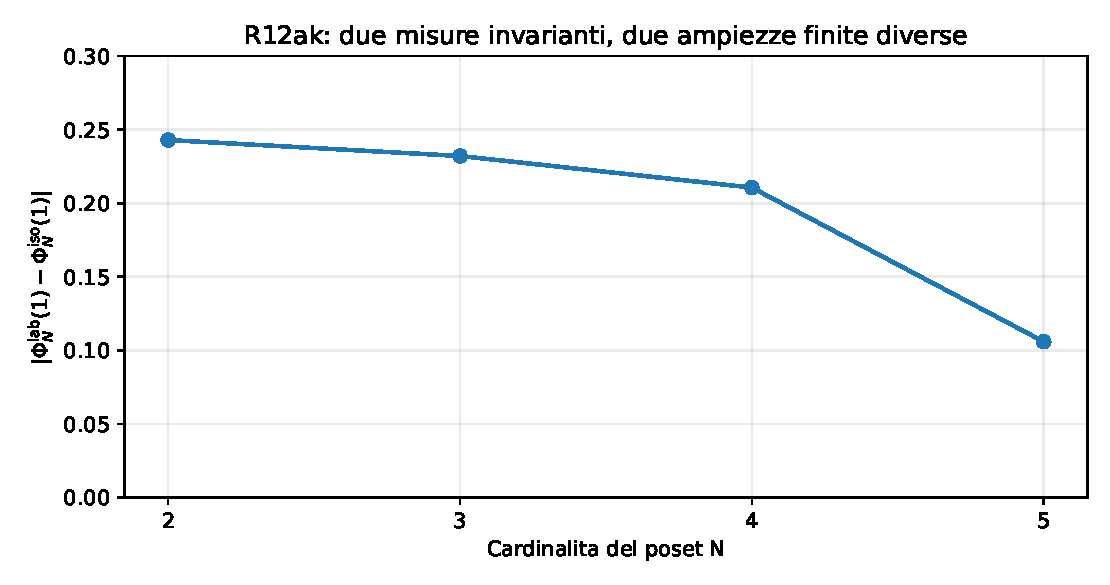
\includegraphics[width=0.66\linewidth]{r12ak_measure_difference.pdf}
\caption{Differenza, a $g=1$ diagnostico, fra le funzioni caratteristiche dei due pesi di riferimento. L'esistenza di due risultati diversi e dimostrata gia da Eq.~\eqref{eq:r12ak_n2}; i punti $N=3,4,5$ sono enumerazioni esatte e non stabiliscono una legge asintotica.}
\label{fig:r12ak_measure_difference}
\end{figure}

\subsection{Perche neppure Ward e crescita sequenziale selezionano qui la fisica}

Una identita di Ward gravitazionale \emph{on shell} richiederebbe un funzionale dinamico diffeomorfismo-invariante $\Gamma[g,\phi]$, un operatore di sorgente e delle equazioni per i campi. Con la convenzione $\delta\Gamma=\int\sqrt{-g}\,(\tfrac12T^{\mu\nu}\delta g_{\mu\nu}+E_\phi\delta\phi)$, l'invarianza sotto diffeomorfismi implica formalmente
\begin{equation}
 \nabla_\mu T^{\mu}{}_{\nu}=E_\phi\nabla_\nu\phi,
 \qquad E_\phi=0\Longrightarrow\nabla_\mu T^{\mu}{}_{\nu}=0.
 \label{eq:r12ak_ward}
\end{equation}
Ma questa condizione non sceglie univocamente $\Gamma$: per esempio la famiglia di \emph{azioni di confronto}, non proposta come teoria causal-set,
$\Gamma_\xi=-\tfrac12\int\sqrt{-g}\,[(\nabla\phi)^2+\xi R\phi^2]$ e diffeomorfismo-invariante per ogni $\xi$, eppure modifica le equazioni di moto e lo stress. Nessuna variazione metrica e stata aggiunta all'azione combinatoria di R12aj attraverso questo esempio.

Esistono inoltre modelli di crescita sequenziale classica conformi a principi di causalita e covarianza discreta che formano una \emph{famiglia di dinamiche}, non una legge unica \cite{RideoutSorkin2000}. Un lavoro sulla causalita di Bell nella crescita \emph{quantistica} pubblicato il 7 ottobre 2026 ricava nuovi vincoli sugli operatori di transizione, ma non una loro costruzione generale computabile \cite{SrivastavaSurya2026}; il risultato non fornisce il missing stress/response del nostro modello. Tali riferimenti sono \emph{benchmark della letteratura}, non risultati originali di R12ak.

\subsection{Decisione R12ak: no-go ristretto, blocco fisico non aggirato}

\begin{center}\small
\begin{tabular}{p{0.45\linewidth}p{0.19\linewidth}p{0.27\linewidth}}
\toprule
\textbf{Requisito} & \textbf{Esito} & \textbf{Ambito del controllo}\\\midrule
Spazio e azione combinatoria finite & \status{PASS} & $N=1,\ldots,5$, $B_N$ esatto.\\
Rietichettatura invariata & \status{PASS} & Entrambi i pesi rispettano la simmetria.\\
Misura selezionata da sola invarianza & \status{FAIL} & Controesempio $N=2$ esatto; enumerazione fino a $5$.\\
Dinamica Lorentziana 4d su geometrie fisiche & \status{NON DERIVATA} & I poset generali non definiscono dimensione, bordo e limite.\\
Sorgente conservata e Ward on-shell & \status{NON DEFINITA} & Nessun $\Gamma[g,\phi]$ derivato dall'azione discreta.\\
Noise e risposta retarded / CTP & \status{NON DEFINITI} & Nessuna costruzione dinamica di stress.\\
Chiusura $H(t)$ e Gate R13 & \status{BLOCCATI} & Nessuna legge cosmologica indipendente.\\
\bottomrule
\end{tabular}
\end{center}

\textbf{Verdetto.} La coppia ``azione BDG + invarianza per rietichettatura'' \emph{non seleziona una misura unica}. Il risultato e limitato a una non-unicita di \emph{pesi di riferimento finite-$N$}; non e una dimostrazione che una teoria fisica completa non possa selezionare la misura mediante principi ulteriori. Il candidato R12aj resta a background imposto; il completamento fisico non puo essere introdotto assegnando arbitrariamente un peso o scegliendo $H(t)$ dopo il fatto. Si congela pertanto la classificazione
\begin{center}\small
\nolinkurl{R12AK_FINITE_MEASURE_NONUNIQUENESS_PASS_PHYSICAL_SELECTION_NOT_DERIVED_R13_BLOCKED}.
\end{center}
\textbf{Decisione strategica:} non autorizzare una catena indefinita di gate computazionali nel ramo 4d. Una nuova fase microdinamica richiedera un \emph{principio indipendente e dichiarato} che fissi almeno spazio delle storie, misura quantistica, variabili dinamiche, stress conservato, risposta e limite continuo. Finche manca, \textbf{R13 rimane BLOCCATO}.


\section{Gate R12al: crescita causale classica, liberta della misura e test di dimensionalita}
\label{sec:r12al}

\textbf{Portata del gate condizionale.} Dopo R12ak non e autorizzata una nuova misura quantistica scelta a mano. R12al esamina invece un candidato \emph{indipendente e preesistente}: la \emph{classical sequential growth} (CSG) di Rideout e Sorkin. Le condizioni di temporalita interna, covarianza discreta, causalita di Bell e regola di somma di Markov vincolano fortemente il processo, ma la soluzione nota e una \emph{famiglia} di dinamiche classiche, non un principio di selezione univoco della misura quantistica \cite{RideoutSorkin2000,VaradarajanRideout2006}. Lo scopo e verificare due blocchi gia identificati: liberta della misura e dimensionalita geometrica. Il protocollo \texttt{R12AL\_PREREGISTRATION.json}, congelato prima della produzione numerica, fissa esempi $p=1/4,1/2,3/4$, enumerazione esaustiva di reti di legami per $N=2,\ldots,5$ e diagnostica $N=8,\ldots,256$. Non sono effettuati fit.

\subsection{Una soluzione classica esplicita: percolazione transitiva}

Siano $0,1,\ldots,N-1$ le etichette \emph{naturali} d'ordine di nascita. Ogni coppia $i<j$ riceve indipendentemente un legame $i\to j$ con probabilita $p\in(0,1)$, \emph{costante lungo la crescita}; il causal set finale e la chiusura transitiva del grafo diretto. Questa e la percolazione transitiva, una soluzione particolare classica nota del programma CSG \cite{RideoutSorkin2000}. L'uso di etichette per calcolare non attribuisce un significato fisico all'ordine arbitrario dei nati incomparabili.

Sia $L(C)$ il numero di \emph{cover relations} (links nel diagramma di Hasse), e sia $I(C)$ il numero di coppie non confrontabili. Per ogni ordine naturalmente etichettato $C$ si ottiene \emph{esattamente}
\begin{equation}
 \mathbb P_p(C)=p^{L(C)}(1-p)^{I(C)}.
 \label{eq:r12al_probability}
\end{equation}
\textbf{Dimostrazione.} Ogni relazione di copertura deve corrispondere a un legame diretto, poiche non puo risultare da un cammino con nodi intermedi; tutti i legami su coppie incomparabili devono essere assenti. Su una coppia comparabile non di copertura il legame diretto e invece libero: la chiusura transitiva delle coperture assicura gia la relazione. Sommando le due possibilita $p+(1-p)=1$ per ciascuna coppia libera si ottiene la Eq.~\eqref{eq:r12al_probability}. Poiche $L$ e $I$ non cambiano passando a un'altra etichettatura naturale dello stesso poset, la probabilita del cammino completo e indipendente da quella scelta. Cio \emph{non} costituisce una dimostrazione indipendente di tutte le condizioni CSG, gia trattate nella letteratura.

\subsection{La simmetria piu forte non sceglie $p$}

A $N=2$ esistono catena $C_2$ e anticatena $A_2$, con $\mathbb P_p(C_2)=p$ e $\mathbb P_p(A_2)=1-p$. Come \emph{osservabile diagnostico, non come misura quantistica di crescita}, applichiamo alle due probabilita classiche la stessa fase BDG 4d usata in R12aj--R12ak: $a_{\rm BDG}=4/\sqrt6$, $B_2(C_2)=1$, $B_2(A_2)=2$. Segue
\begin{align}
 \Phi^{\rm diag}_2(p;g)&=p\,e^{iga_{\rm BDG}}+(1-p)e^{2iga_{\rm BDG}},\\
 \bigl|\Phi^{\rm diag}_2(p;g)-\Phi^{\rm diag}_2(p';g)\bigr|
 &=2|p-p'|\left|\sin\frac{ga_{\rm BDG}}2\right|.
 \label{eq:r12al_nonunique}
\end{align}
Al valore \emph{preregistrato} $g=1$, $p=1/4$ e $p'=3/4$ differiscono di $0.728751240810\ldots$. E una distinzione analitica, non una inferenza statistica: anche all'interno di questa famiglia conforme ai vincoli classici, essi non selezionano un valore unico di $p$. L'ampiezza qui non e una \emph{quantum sequential growth measure}: inserire una fase BDG in una probabilita classica non fornisce automaticamente una decoherence functional estendibile, una dinamica unitaria o una Ward gravitazionale. La ricerca sulla causalita di Bell quantistica lascia vincoli non banali e una rappresentazione generale non costruita \cite{SrivastavaSurya2026}.

\subsection{Test geometrico: un no-go ristretto a $p$ fisso}

Definiamo il rapporto d'ordine $r_N=R_N/\binom N2$, dove $R_N$ conta le coppie comparabili della chiusura transitiva. Consideriamo $i<j$, con $d=j-i$. Se i due eventi sono incomparabili, manca necessariamente il legame diretto $i\to j$ e, per ogni $k$ intermedio, manca almeno uno dei due legami diretti $i\to k$, $k\to j$. Gli eventi di mancanza di questi cammini di lunghezza due coinvolgono coppie di legami distinte e sono indipendenti. Pertanto
\begin{equation}
 \mathbb P_p(i\not\prec j)\le(1-p)(1-p^2)^{j-i-1}.
 \label{eq:r12al_pair_bound}
\end{equation}
La disuguaglianza, non necessariamente un'uguaglianza, esclude anche i cammini di lunghezza maggiore; non assume che tutti gli eventi di comparabilita siano indipendenti. Sommando per distanza tra etichette,
\begin{align}
 \mathbb E_p(1-r_N)&\le \frac{2(1-p)}{N(N-1)}
 \sum_{d=1}^{N-1}(N-d)(1-p^2)^{d-1}\\
 &\le \frac{2(1-p)}{p^2(N-1)}.
 \label{eq:r12al_order_bound}
\end{align}
Per \emph{ogni} $p$ fissato in $(0,1)$, la Eq.~\eqref{eq:r12al_order_bound} dimostra $r_N\to1$ in $L^1$ e in probabilita, applicando Markov a $1-r_N\ge0$. Al contrario, per $N$ punti iid condizionati in un \emph{diamante di Minkowski 4d}, il valore medio della frazione d'ordine e il riferimento Myrheim--Meyer \cite{Surya2019Review}
\begin{equation}
 \mathbb E[r_N\mid \mathbb M^4\text{ diamond}]
 =\frac{\Gamma(5)\Gamma(2)}{2\Gamma(6)}=\frac1{10}.
 \label{eq:r12al_4d_reference}
\end{equation}
Quindi una sequenza di prefissi di \emph{percolazione transitiva a $p$ costante} non puo riprodurre quel valore di confronto quadridimensionale quando $N\to\infty$. Questo e un \textbf{no-go ristretto} per tale baseline, \emph{non} per altri parametri CSG, cambi di scala, leggi quantistiche o geometrie FLRW curve. Il confronto $1/10$ e specifico del diamante piatto e non costituisce una predizione universale della cosmologia.

\subsection{Enumerazioni, controlli indipendenti e diagnostica}\label{subsec:r12al_valid}
La formula delle probabilita e stata confrontata con l'enumerazione di \emph{tutte le reti di legami} per $N=2,3,4,5$, a $p=1/4$ e $3/4$: rispettivamente $2,7,40,357$ poset naturalmente etichettati distinti. Le probabilita razionali, le normalizzazioni e il bound finito sono state verificate. Un secondo programma, che usa una matrice booleana e chiusura di Warshall anziche maschere di predecessori, ha ripetuto i confronti. Il programma principale registra 38/38 verifiche superate e il replay indipendente 52/52; un errore nella prima asserzione del smoke-test, corretto prima della produzione, e documentato in \texttt{R12AL\_TECHNICAL\_AMENDMENT.md}.

\begin{table}[htbp]\centering\small
\caption{R12al: media della frazione comparabile su 128 realizzazioni per ciascuna coppia $(N,p)$, con semi congelati. Numeri diagnostici e non stime di un esponente asintotico; la convergenza a 1 e dimostrata separatamente da Eq.~\eqref{eq:r12al_order_bound}.}
\label{tab:r12al_mc}
\begin{tabular}{rccc}\toprule
$N$&$p=1/4$&$p=1/2$&$p=3/4$\\\midrule
32&0.663574&0.905289&0.974310\\
256&0.949469&0.987544&0.996675\\\bottomrule
\end{tabular}
\end{table}
\begin{figure}[htbp]\centering
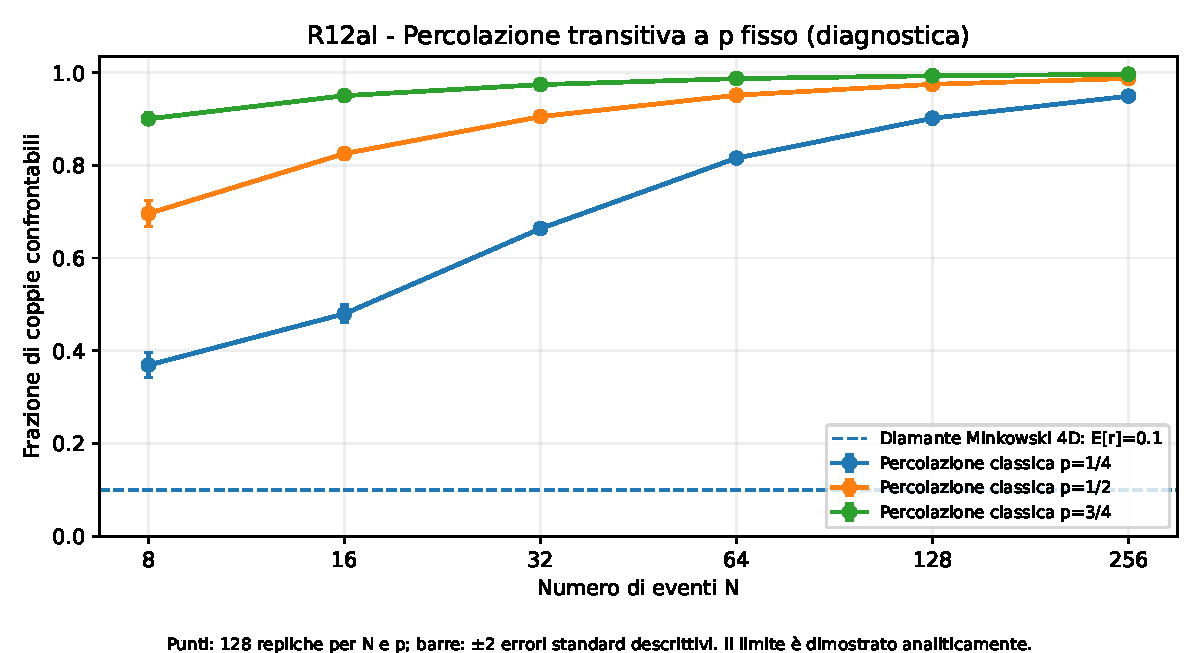
\includegraphics[width=0.91\linewidth]{r12al_comparability.pdf}
\caption{Confronto diagnostico di percolazione transitiva classica a parametro fisso con il valore d'ordine del diamante piatto 4d. Le barre sono $\pm2$ errori standard \emph{descrittivi}, senza usarle come prova del limite o come criterio di selezione di $p$.}
\label{fig:r12al_comparability}
\end{figure}

\subsection{Verdetto fisico e condizione per riaprire il progetto}

\textbf{Risultati del gate:} (i) un candidato classico indipendente e non banale esiste e la sua liberta di parametro e esplicita; (ii) l'osservabile $N=2$ distingue esattamente due valori del parametro; (iii) la baseline a $p$ fisso possiede un limite di frazione comparabile incompatibile con il benchmark di diamante Minkowski 4d. Nessuno di questi tre esiti costruisce un peso quantistico fisico 4d. Mancano ancora una legge quantistica selezionata, il settore metrico dinamico e la Ward on-shell, rumore e risposta retarded, condizioni al bordo, limite continuo e chiusura $H(t)$. In particolare il \textbf{Gate R13 resta bloccato}.

\begin{center}\small\nolinkurl{R12AL_EXTERNAL_CLASSICAL_GROWTH_AUDIT_PASS_FIXED_P_4D_DIAMOND_MISMATCH_QUANTUM_CLOSURE_NOT_DERIVED_R13_BLOCKED}\end{center}

\textbf{Decisione strategica:} non promuovere questa baseline a teoria fisica e non cercare di ``ripararla'' scegliendo $p(N)$ dopo aver visto i dati. Un nuovo esperimento sarebbe giustificato soltanto da una legge di scala/misura quantistica motivata indipendentemente, con dimensionalita, conservazione, risposta e continuum verificabili. In mancanza di tale principio si preserva il risultato come audit ristretto e si sospende l'estensione automatica.


\section{Gate R12am: crescita quantistica a cilindri finiti, non-unicita e compatibilita con BDG}
\label{sec:r12am}

\textbf{Riapertura condizionale e prior art.} Dopo il no-go ristretto per la percolazione \emph{classica} a parametro fisso di R12al, si esamina una costruzione quantistica \emph{gia nota}: la \emph{complex percolation} dei causal set \cite{Gudder2012QuantumGrowth,DowkerJohnstonSurya2010}. La ricerca recente sulle identita di Bell quantistiche esplicita il diverso e piu difficile problema dei generatori non commutativi \cite{SrivastavaSurya2026}. Il protocollo \texttt{R12AM\_PREREGISTRATION.json} fissa prima dei risultati due valori diagnostici di un parametro \emph{complesso}; non e una selezione microfisica e non contiene fit cosmologici.

\subsection{Ampiezze naturali e regola di crescita}
Sia $\Omega_n^{\mathrm{nat}}$ l'insieme dei poset transitivi naturalmente etichettati da $0$ a $n-1$. Indichiamo con $L(C)$ il numero delle coppie di copertura e con $I(C)$ il numero delle coppie incomparabili. Per $z\in\mathbb C$ e $q_z=1-z$ poniamo
\begin{equation}
 {\cal A}_{z,n}(C)=z^{L(C)}q_z^{I(C)}.
 \label{eq:r12am_amplitude}
\end{equation}
Una crescita $C\to C_P$ aggiunge un nuovo elemento massimale il cui passato e un ideale d'ordine $P\subseteq C$. Posti $\omega=|P|$ e $m(P)$ uguale al numero di massimali di $P$, si ha
\begin{equation}
 t_z(C\to C_P)=z^{m(P)}q_z^{n-\omega},\qquad
 {\cal A}_{z,n+1}(C_P)={\cal A}_{z,n}(C)\,t_z(C\to C_P).
 \label{eq:r12am_transition}
\end{equation}
\textbf{Verifica algebrica.} Consideriamo tutte le $2^n$ configurazioni dei legami entranti al nuovo punto. La somma delle ampiezze dei singoli legami presenti/assenti e $z+q_z=1$, quindi la somma di tutte le configurazioni vale uno. Per produrre un dato passato $P$, i $m(P)$ legami dai suoi massimali sono obbligatori e i $n-\omega$ legami dall'esterno sono assenti; i restanti $\omega-m(P)$ legami, ridondanti per la chiusura transitiva, si sommano a $(z+q_z)^{\omega-m(P)}=1$. Ne segue l'identita esatta
\begin{equation}
 \sum_{P\text{ ideale di }C}t_z(C\to C_P)=1,\qquad
 \sum_{C\in\Omega_n^{\mathrm{nat}}}{\cal A}_{z,n}(C)=1.
 \label{eq:r12am_norm}
\end{equation}
La dipendenza dai soli $L$ e $I$ e invariante sotto rietichettature \emph{naturali}; non costituisce da sola una definizione priva di ambiguita del peso degli ordini non etichettati.

\subsection{Decoerenza forte e consistenza dei cilindri}
Per eventi finiti $E,F\subseteq\Omega_n^{\mathrm{nat}}$ definiamo
\begin{equation}
 a_{z,n}(E)=\sum_{C\in E}{\cal A}_{z,n}(C),\qquad
 D_{z,n}(E,F)=a_{z,n}(E)\,\overline{a_{z,n}(F)},\qquad
 \mu_{z,n}(E)=D_{z,n}(E,E).
 \label{eq:r12am_D}
\end{equation}
Per qualsiasi famiglia finita di eventi $E_j$ e coefficienti complessi $c_j$,
\begin{equation}
 \sum_{j,k}\overline{c_j}D_{z,n}(E_j,E_k)c_k
 =\left|\sum_j\overline{c_j}a_{z,n}(E_j)\right|^2\ge0.
 \label{eq:r12am_positive}
\end{equation}
Il funzionale e dunque hermitiano, biadditivo, normalizzato $D(\Omega_n,\Omega_n)=1$ e \emph{fortemente positivo}. La Eq.~\eqref{eq:r12am_norm} implica la compatibilita tra stadi delle ampiezze degli eventi cilindrici. Non e stata invece verificata l'\emph{estensione all'intera sigma-algebra} delle storie infinite. Questo e un vero problema aggiuntivo: sono noti esempi che non si estendono e anche famiglie per cui l'estensione e dimostrabile \cite{DowkerJohnstonSurya2010,SuryaZalel2020}.

\subsection{Due dinamiche distinte con gli stessi vincoli finiti}
A $n=2$, con $C_2$ catena e $A_2$ anticatena,
\begin{equation}
 \mu_z(C_2)=|z|^2,\quad \mu_z(A_2)=|1-z|^2,\quad
 {\cal I}_2(z)=1-\mu_z(C_2)-\mu_z(A_2)
 =2\operatorname{Re}[z\overline{(1-z)}].
 \label{eq:r12am_n2}
\end{equation}
A differenza di una probabilita classica, qui $\mu(C_2)+\mu(A_2)$ non deve essere uno: la differenza e esattamente l'interferenza. Con i due valori fissati prima dei risultati si ottiene la Tab.~\ref{tab:r12am_quantum}.
\begin{table}[htbp]\centering\small
\caption{R12am: misure quantistiche esatte a due elementi. Tutti i valori sono razionali gaussiani calcolati senza Monte Carlo; in entrambe le righe $\mu(\Omega_2)=1$.}
\label{tab:r12am_quantum}
\begin{tabular}{lccc}\toprule
$z$&$\mu(C_2)$&$\mu(A_2)$&${\cal I}_2$\\\midrule
$\frac14+\frac{i}{8}$ & $\frac5{64}$ & $\frac{37}{64}$ & $\frac{11}{32}$\\
$\frac12+\frac{i}{8}$ & $\frac{17}{64}$ & $\frac{17}{64}$ & $\frac{15}{32}$\\\bottomrule
\end{tabular}
\end{table}
\begin{figure}[htbp]\centering
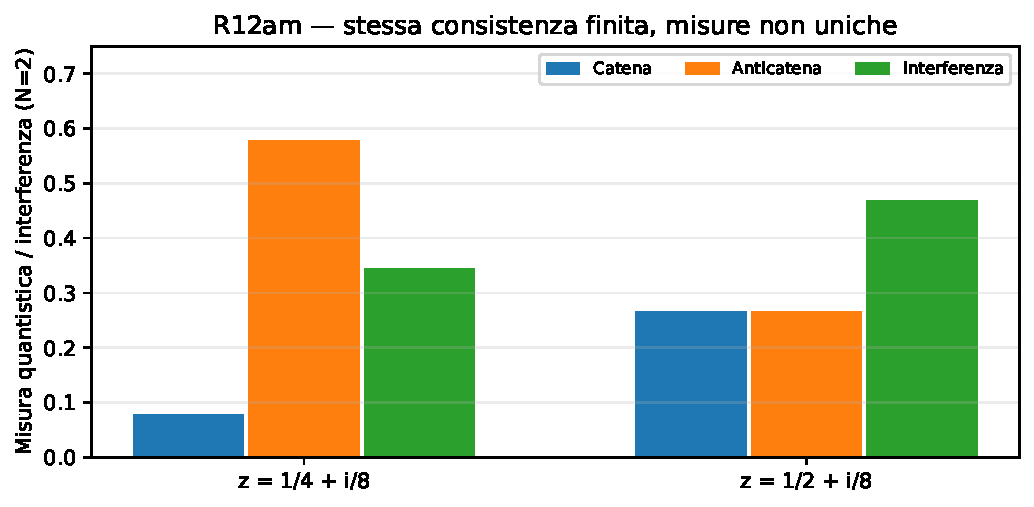
\includegraphics[width=0.81\linewidth]{r12am_quantum_measure.pdf}
\caption{Differenti misure quantistiche e interferenze a $N=2$ all'interno della stessa famiglia finita di complex percolation. Le tre barre sommano a uno includendo l'interferenza, non sono probabilita classiche di eventi esclusivi.}
\label{fig:r12am_quantum}
\end{figure}
L'assenza di unicita e gia analitica a due eventi. \textbf{Non} stiamo risolvendo la forma generale dei generatori operatoriali di quantum Bell causality: il modello a parametri scalari e commutativo. Lo studio di Srivastava--Surya (2026) trova che due ordinamenti naturali forzano tale commutativita sotto ipotesi di non-singolarita, mentre un terzo ordinamento impone ulteriori relazioni senza determinare una rappresentazione generale \cite{SrivastavaSurya2026}.

\subsection{Controesempio alla moltiplicazione terminale per la fase BDG}
Una fusione apparentemente minimale con R12aj sarebbe assegnare a ogni stadio
\begin{equation}
 \widetilde {\cal A}_{z,n}(C)=c_n\,{\cal A}_{z,n}(C)
 \exp\bigl[igS_{\rm BDG}(C)\bigr],
 \label{eq:r12am_terminal_phase}
\end{equation}
con $c_n$ \emph{indipendente dalla storia}. Per rendere consistenti i cilindri, il rapporto
\begin{equation}
 F_z(C)=\frac{\sum_{C'\succ C}t_z(C\to C')\exp[igS_{\rm BDG}(C')]}
 {\exp[igS_{\rm BDG}(C)]}
 \label{eq:r12am_F}
\end{equation}
deve essere lo stesso per tutti i genitori allo stadio $n$, perche $F_z(C)=c_n/c_{n+1}$. Nel \emph{toy} BDG a $n=2\to3$, con coefficiente storico $a_4=4/\sqrt6$ e $g=1$, il conteggio esatto degli intervalli fornisce
\begin{align}
 F_z(C_2)&=q_z^2e^{ia_4}+zq_z+ze^{9ia_4},\\
 F_z(A_2)&=q_z^2e^{ia_4}+2zq_z+z^2e^{-ia_4}.
 \label{eq:r12am_parent_F}
\end{align}
Le differenze $|F_z(C_2)-F_z(A_2)|$ sono rispettivamente $0.51876949$ e $0.95768775$ per i due parametri congelati. Di conseguenza \textbf{nessun unico fattore $c_{n+1}/c_n$ dipendente soltanto da $n$ ripristina la consistenza per entrambi i genitori}. Il controesempio riguarda \emph{questa prescrizione terminale}, non l'impossibilita di incorporare un'azione gravitazionale in una regola piu ricca per le transizioni.

\subsection{Verifiche indipendenti e verdetto}
Il replay ha enumerato tutte le taglie $n=1,\ldots,6$ (rispettivamente $1,2,7,40,357,4824$ poset naturalmente etichettati) e superato $1719$ controlli nel programma principale. Un secondo programma, basato sulle reti di legami orientati e sulla chiusura transitiva senza riutilizzare il generatore principale, ha superato $1402$ controlli addizionali, compresi i confronti di ampiezze \emph{esatte} a $n\le5$. Il controesempio BDG e stato ricalcolato con una formula chiusa indipendente. Entrambi gli esiti positivi sono \emph{di dimensione finita}.

\begin{center}\small\texttt{R12AM\_FINITE\_CYLINDER\_PASS\_MEASURE\_NOT\_SELECTED}\end{center}
\begin{center}\small\texttt{BDG\_TERMINAL\_PHASE\_FAIL\_FULL\_EXTENSION\_OPEN\_R13\_BLOCKED}\end{center}
Non sono stati costruiti una dinamica gravitazionale 4D, un tensore sorgente con identita di Ward on-shell, una risposta CTP retarded o un limite continuo fisico. \textbf{R13 resta bloccato}. Qualsiasi nuovo gate deve essere motivato prima da un \emph{principio indipendente} di scelta della misura e di accoppiamento dinamico; non sara autorizzato un altro valore di $z$ scelto retrospettivamente.


\section{Gate R12an: normalizzazione locale della fase BDG e coerenza delle storie causali}
\label{sec:r12an}

\textbf{Problema e protocollo.} Il Gate R12am ha verificato che aggiungere il fattore terminale $\exp(igS_{\rm BDG})$ alla percolazione complessa preesistente rompe, in generale, la coerenza dei cilindri \cite{Gudder2012QuantumGrowth,DowkerJohnstonSurya2010}. R12an testa una possibile riparazione \emph{senza modificare} i due parametri $z_A=1/4+i/8$, $z_B=1/2+i/8$, il coupling diagnostico $g=1$ e l'azione finita $S_n=a_4s_n$, $a_4=4/\sqrt 6$, $s_n=n-N_0+9N_1-16N_2+8N_3$. La domanda e se una normalizzazione \emph{per ogni genitore} possa rendere i pesi consistenti e contemporaneamente conservare la stessa ampiezza per due etichettature naturali di un unico poset non etichettato. Il protocollo \texttt{R12AN\_PREREGISTRATION.json} e stato congelato prima del calcolo principale; nessun parametro e stato fittato ai dati.

\subsection{La riparazione a un passo e un'identita di normalizzazione}
Con $t_z(C,C')$ definita in Eq.~\eqref{eq:r12am_transition}, poniamo
\begin{equation}
 F_z(C):=\sum_{C'\succ C}t_z(C,C')\exp\!\bigl[ig(S(C')-S(C))\bigr], \qquad
 \widehat t_z(C,C'):=\frac{t_z(C,C')\exp[ig(S(C')-S(C))]}{F_z(C)},
 \label{eq:r12an_local_transfer}
\end{equation}
quando $F_z(C)\neq0$. Per costruzione $\sum_{C'\succ C}\widehat t_z(C,C')=1$, cosicche le ampiezze dei cilindri a $n$ finito sono consistenti. Questa proprieta e una \emph{normalizzazione algebrica}, non una dimostrazione di fisica unitaria o della corretta misura sull'insieme delle geometrie.

\subsection{Controesempio esatto: due storie dello stesso ordine a tre elementi}
Siano $C_2$ la catena a due punti e $A_2$ l'anticatena. Aggiungendo un punto isolato a $C_2$, oppure un punto sopra uno dei due elementi di $A_2$, si ottengono \emph{due storie naturalmente etichettate isomorfe}: un legame e un punto isolato. Entrambe hanno ampiezza di base $z(1-z)^2$ e la stessa azione terminale. Il fattore comune dello stadio $n=1$ si cancella nel rapporto; la riparazione locale invece fornisce
\begin{equation}
 \frac{\widehat{\mathcal A}_z(C_3^{\mathrm{catena\ prima}})}
 {\widehat{\mathcal A}_z(C_3^{\mathrm{anticatena\ prima}})}
 =\frac{F_z(A_2)}{F_z(C_2)}.
 \label{eq:r12an_covariance_ratio}
\end{equation}
Per il conteggio BDG storico, Eq.~\eqref{eq:r12am_parent_F},
\begin{equation}
 F_z(C_2)-F_z(A_2)=z\Bigl[e^{9ia_4}-(1-z)-ze^{-ia_4}\Bigr].
 \label{eq:r12an_diamond_obstruction}
\end{equation}
Questa espressione non si annulla per nessuno dei due valori $z$ preregistrati. Ne segue un \textbf{no-go ristretto}: la normalizzazione \emph{solo al genitore} della Eq.~\eqref{eq:r12an_local_transfer} ripristina i cilindri ma viola l'uguaglianza delle ampiezze tra due storie che rappresentano lo stesso poset. Non e un teorema sulla impossibilita di ogni dinamica quantistica o di ogni scelta di $z$.

\subsection{Riparazione alternativa con funzione di partizione a ritroso}
Esiste un rimedio algebrico finito, che tuttavia richiede una nuova scelta di bordo. Per un orizzonte terminale discreto $H$, si fissi $h_H^{(H)}(C)=1$ e, ricorsivamente,
\begin{equation}
 h_n^{(H)}(C)=\sum_{C'\succ C}t_z(C,C')\exp\!\bigl[ig(S(C')-S(C))\bigr]h_{n+1}^{(H)}(C'),\quad n<H.
 \label{eq:r12an_backward_recursion}
\end{equation}
Quando i denominatori sono non nulli, il trasferimento corretto
\begin{equation}
 t_z^{(H)}(C,C')=\frac{t_z(C,C')e^{ig(S(C')-S(C))}h_{n+1}^{(H)}(C')}{h_n^{(H)}(C)}
 \label{eq:r12an_future_transfer}
\end{equation}
ha somma unitaria sui successori. Le ampiezze risultanti possono essere scritte in forma terminale
\begin{equation}
 {\mathcal A}_{z,n}^{(H)}(C)=
 \frac{{\mathcal A}_{z,n}(C)e^{igS(C)}h_n^{(H)}(C)}{h_0^{(H)}(\varnothing)},
 \label{eq:r12an_future_amplitude}
\end{equation}
e dipendono soltanto dalla classe di isomorfismo del poset a $n$ fissato: dunque sono compatibili con i cilindri e con la \emph{invarianza finita delle ampiezze sotto etichettatura naturale}. Ma $h_n^{(H)}$ somma esplicitamente le possibili prosecuzioni \emph{fino al bordo futuro $H$}; non e una regola microfisica selezionata dal solo passato causale. Inoltre il valore di una stessa ampiezza cilindrica cambia in generale quando si cambia $H$.

\subsection{Controlli numerici e limiti della conclusione}
La Tab.~\ref{tab:r12an_diagnostics} registra tre misure \emph{diverse}: lo scarto dei normalizzatori di genitore, il difetto di uguaglianza tra le due etichettature naturali, e il cambiamento dell'ampiezza del cilindro $C_2$ tra $H=3$ e $H=4$. Indichiamo queste colonne rispettivamente con $\Delta F$, $\Delta_{\rm label}$ e $\Delta_H$. Nessuna cifra e un fit cosmologico.
\begin{table}[htbp]\centering\small
\caption{R12an: diagnostiche finite ai parametri congelati $g=1$ e $a_4=4/\sqrt6$.}\label{tab:r12an_diagnostics}
\begin{tabular}{lrrr}\toprule
Parametro $z$ & $\Delta F$ & $\Delta_{\rm label}$ & $\Delta_H$\\\midrule
$1/4+i/8$ & 0.518769 & 0.130149 & 0.099872\\
$1/2+i/8$ & 0.957688 & 0.335875 & 0.475207\\\bottomrule
\end{tabular}
\end{table}
\begin{figure}[htbp]\centering
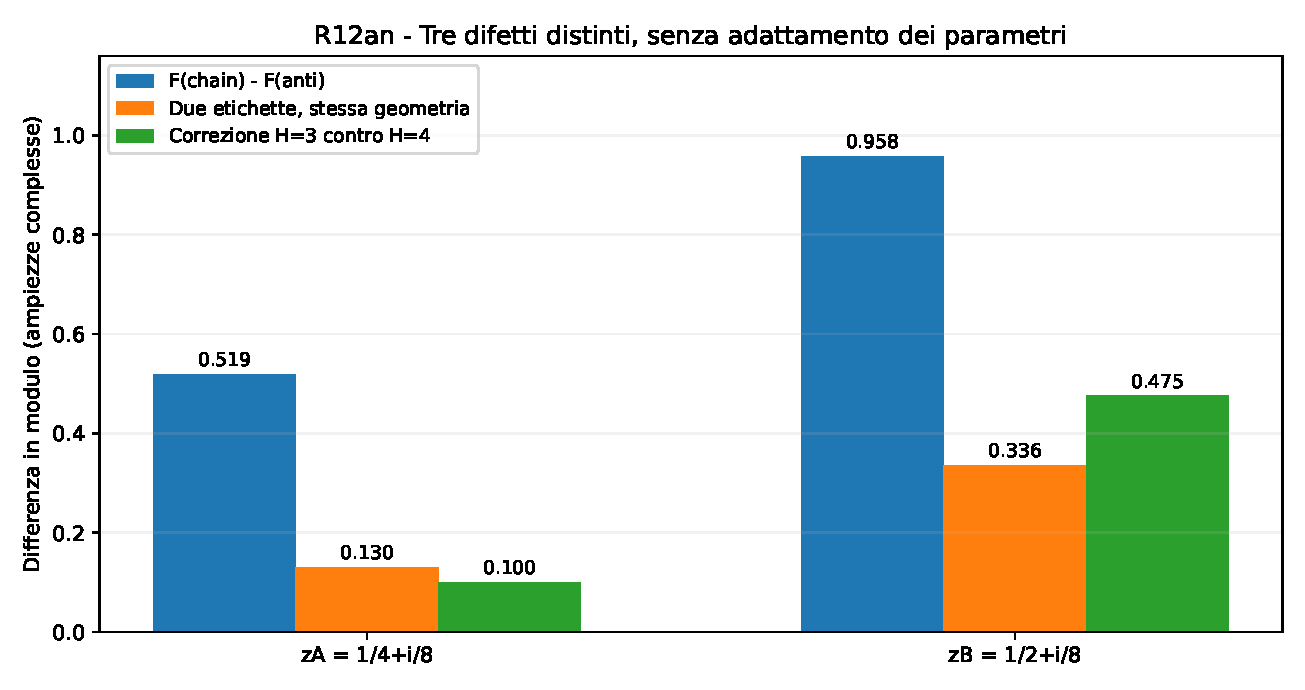
\includegraphics[width=0.88\linewidth]{r12an_local_boundary_diagnostics.pdf}
\caption{Tre differenze in modulo, senza variare i parametri storici. La riparazione locale normalizza i cilindri ma distingue due etichette naturali isomorfe; la riparazione con bordo futuro dipende dall'orizzonte scelto.}
\label{fig:r12an_diagnostics}
\end{figure}
Il programma principale supera \textbf{258/258} verifiche, fra cui le $102$ normalizzazioni dei genitori fino allo stadio $4$, le ricorrenze e le ampiezze finite con $H=3,4$; l'enumeratore indipendente per chiusura transitiva di grafi supera \textbf{18/18} confronti addizionali fino a $n=4$. Sono calcoli \emph{finiti} con errori di floating point sotto le soglie preregistrate; l'ostacolo in Eq.~\eqref{eq:r12an_diamond_obstruction} e algebrico.

\textbf{Prior art e delimitazione fisica.} La questione della estensione della misura sugli eventi infiniti e distinta dalla invarianza di un'ampiezza finita \cite{DowkerJohnstonSurya2010,SuryaZalel2020}. L'implementazione non commutativa della quantum Bell causality rappresenta una ulteriore struttura non risolta dal presente modello scalare \cite{SrivastavaSurya2026}. La riparazione a ritroso e un'identita di \emph{partition function} condizionata a un bordo, non una derivazione della selezione di $z$, di un'azione gravitazionale dinamica, di un tensore sorgente Ward, della risposta retarded o del limite continuo.

\begin{center}\small\texttt{R12AN\_LOCAL\_NORMALIZATION\_GC\_FAIL}\end{center}
\begin{center}\small\texttt{FUTURE\_HORIZON\_REPAIR\_FINITE\_PASS\_PHYSICAL\_SELECTION\_OPEN}\end{center}
\textbf{Decisione:} senza una legge fisica indipendente che scelga misura, ampiezze, bordi e limite 4D, il Gate R13 resta \textbf{BLOCCATO}. Non si autorizza un nuovo fit di $z$, $g$, o del bordo $H$ per aggirare il controesempio.

\section{Gate R12ao: fase BDG come cobordo esatto e limite della selezione armonica}
\label{sec:r12ao}

\textbf{Obiettivo e perimetro.} Il Gate R12an ha mostrato due fatti apparentemente in tensione: una normalizzazione locale della fase d'azione puo rompere la covarianza delle ampiezze, mentre una riparazione con funzione di partizione a ritroso richiede un bordo futuro. R12ao affronta ora la struttura comune di questi risultati, senza introdurre nuove costanti o adattare i dati. Il protocollo \texttt{R12AO\_PREREGISTRATION.json} conserva i valori diagnostici $g=1$, $z_A=1/4+i/8$, $z_B=1/2+i/8$ e l'azione BDG $S_n=a_4[n-N_0+9N_1-16N_2+8N_3]$, $a_4=4/\sqrt6$. Il risultato riguarda le \emph{ampiezze di crescita finita} e non costituisce una selezione della misura quantistica fisica in 4d.

\subsection{Cobordo esatto della differenza d'azione}
Siano ${\cal C}_n$ gli ordini causali naturalmente etichettati di $n$ eventi e $t_z(C,C')$ le ampiezze di crescita, gia normalizzate in modo che $\sum_{C'\succ C}t_z(C,C')=1$ (Eq.~\eqref{eq:r12am_transition}). Definiamo il trasferimento fase-deformato
\begin{equation}
 K_{S,n}(C,C')=t_z(C,C')e^{ig[S_{n+1}(C')-S_n(C)]}.
 \label{eq:r12ao_twist}
\end{equation}
Lungo ogni storia $C_0\to C_1\to\cdots\to C_N$ le fasi telescopizzano:
\begin{equation}
 \prod_{j=0}^{N-1}e^{ig[S_{j+1}(C_{j+1})-S_j(C_j)]}
 =e^{ig[S_N(C_N)-S_0(C_0)]}.
 \label{eq:r12ao_telescoping}
\end{equation}
Ponendo $M_nf(C)=e^{igS_n(C)}f(C)$, il trasferimento e \emph{esattamente} coniugato allo stesso trasferimento privo della fase:
\begin{equation}
 \boxed{K_{S,n}=M_n^{-1}K_{0,n}M_{n+1}}.
 \label{eq:r12ao_conjugacy}
\end{equation}
E un'identita fra operatori \emph{graduati}, non una dimostrazione di unitarieta o una gauge equivalence fra due teorie gravitazionali complete. In particolare una somma oscillante terminale $\sum_{C\in{\cal C}_N}{\cal A}_{z,N}(C)e^{igS_N(C)}$ puo essere diversa dalla somma senza fase: il peso d'azione resta osservabile nella \emph{somma a $N$ fissato} quando gli stati finali sono differenti.

\subsection{Normalizzazione cilindrica e cancellazione armonica}
Consideriamo la classe di riparazioni che, per una funzione $h_n(C)\ne0$, assegnano
\begin{equation}
 T_h(C,C')=\frac{K_{S,n}(C,C')h_{n+1}(C')}{h_n(C)}.
 \label{eq:r12ao_h_transform}
\end{equation}
La condizione $\sum_{C'\succ C}T_h(C,C')=1$ e \emph{equivalente}, dove il denominatore esiste, all'equazione di armonicita complessa
\begin{equation}
 h_n(C)=\sum_{C'\succ C}K_{S,n}(C,C')h_{n+1}(C').
 \label{eq:r12ao_harmonic}
\end{equation}
Definendo $u_n(C)=e^{igS_n(C)}h_n(C)$ e utilizzando Eq.~\eqref{eq:r12ao_conjugacy}, la condizione e la transizione si riscrivono
\begin{align}
 u_n(C)&=\sum_{C'\succ C}t_z(C,C')u_{n+1}(C'),\\
 \boxed{T_h(C,C')}&=t_z(C,C')\frac{u_{n+1}(C')}{u_n(C)}.
 \label{eq:r12ao_cancelled}
\end{align}
La fase BDG e \emph{eliminata dal trasferimento normalizzato} all'interno di questa precisa classe. La soluzione piu semplice e $u_n(C)=1$ per ogni stato, poiche $\sum t_z=1$; essa produce $h_n(C)=e^{-igS_n(C)}$ e \emph{esattamente} $T_h=t_z$. Una dinamica normalizzata differente richiede quindi la selezione di una funzione armonica non banale $u$, che l'azione $S$ da sola non determina. Il paragone con la trasformazione di Doob e strutturale \cite{Doob1957}: qui $t_z$ e $u$ possono essere complessi e non si eredita la teoria delle probabilita positive.

\subsection{Il bordo futuro di R12an e un osservabile terminale}
Se si impone il bordo usato in R12an, $h_H^{(H)}(C)=1$, nella rappresentazione senza twist questo corrisponde a
\begin{equation}
 u_H^{(H)}(C)=e^{igS_H(C)},\qquad
 u_n^{(H)}(C)=\sum_{C'\succ C}t_z(C,C')u_{n+1}^{(H)}(C').
 \label{eq:r12ao_terminal_observable}
\end{equation}
L'influenza dell'azione viene quindi portata \emph{dalla condizione terminale}, che somma i futuri possibili, anziche essere selezionata come legge past-only. Il confronto degli stessi cilindri a $H=3$ e $H=4$ riproduce i gap storici di R12an, indicati nella Tab.~\ref{tab:r12ao_checks}.

\subsection{Un'alternativa coerente ma non selezionata}
La non unicita puo essere mostrata senza modificare $S$, $g$ o $z$. Come \emph{sola diagnostica}, al bordo finito $H=4$ scegliamo una funzione di stato invariante sotto rietichettatura
\begin{equation}
 u_4(C)=1+\frac12\,\mathbf 1_{\{C\,\mathrm{catena}\}}.
 \label{eq:r12ao_alt_terminal}
\end{equation}
La propagazione armonica all'indietro e algebricamente risolvibile. Per un prefisso con un evento $u_1=1+z^3/2$; per la catena di due eventi $u_2(C_2)=1+z^2/2$; per l'anticatena $u_2(A_2)=1$. La transizione dalla singola particella alla catena e dunque
\begin{equation}
 T_u(C_1,C_2)=z\frac{1+z^2/2}{1+z^3/2}\ne z.
 \label{eq:r12ao_alt_formula}
\end{equation}
Per entrambi i valori diagnostici di $z$ i denominatori sono non nulli. Questa costruzione conserva normalizzazione e invarianza delle ampiezze finite tra etichettature naturali, ma la scelta di $u_4$ e una \emph{boundary condition aggiuntiva} priva di motivazione microfisica qui derivata. Il fattore $1/2$ non e un fit: e fissato nella preregistrazione solo per esibire una alternativa matematica.

\begin{table}[htbp]\centering\small
\caption{R12ao: controlli finiti ai due parametri complessi gia usati in R12an. $\Delta_H$ e lo scarto del cilindro catena a $N=2$ fra orizzonti futuri $H=3$ e $4$; $\Delta_u=|T_u(C_1,C_2)-z|$ diagnostica la non unicita.}
\label{tab:r12ao_checks}
\begin{tabular}{lrr}\toprule
$z$ & $\Delta_H$ & $\Delta_u$ \\\midrule
$1/4+i/8$ & 0.099872 & 0.008285\\
$1/2+i/8$ & 0.475207 & 0.033541\\\bottomrule
\end{tabular}
\end{table}

\subsection{Verifiche, prior art e verdetto}
L'identita e \emph{analitica}, non inferita dai dati. Il primo programma la controlla sull'intero grafo dei poset naturalmente etichettati fino a $N=5$ (cardinalita $1,1,2,7,40,357$), con \textbf{2404/2404 verifiche PASS}. Un secondo programma \emph{indipendente}, basato sull'enumerazione delle matrici booleane anziche sugli ideali d'ordine, supera \textbf{2463/2463} verifiche, includendo le somme dirette fino al bordo $H=4$. Un errore di sintassi del programma principale corretto \emph{prima di ogni replay valido} e registrato in \texttt{R12AO\_TECHNICAL\_AMENDMENT.md}; i parametri scientifici sono rimasti congelati.

\textbf{Interpretazione.} La coniugazione da cobordo e il principio delle trasformazioni armoniche appartengono a matematica standard, non a una scoperta fisica originale. R12ao mostra che una fase BDG introdotta \emph{solo come differenza di un'azione di stato}, seguita da una riparazione armonica dei cilindri, non seleziona da sola un trasferimento fisico nuovo. Non esclude che un vero path integral su geometrie dinamiche abbia interferenza gravitazionale, che una dinamica non commutativa produca effetti nuovi, o che un principio indipendente scelga la funzione armonica \cite{SuryaZalel2020,SrivastavaSurya2026}.

\textbf{Esito:} \textsf{EXACT COBBOUNDARY/CONJUGACY PASS; PHYSICAL SELECTION NOT DERIVED}. Restano assenti misura quantistica fisica 4d, sorgente Ward/Bianchi dinamica, risposta causale, limite continuo e legge autonoma $H(t)$. Il \textbf{Gate R13 resta BLOCCATO}; non si autorizza un altro sottogate numerico senza una nuova ipotesi microfisica specificata prima dei test.

\section{Gate R12ap: estensione della misura complessa oltre i cilindri finiti}

\textbf{Motivazione e preregistrazione.} Il Gate R12am aveva costruito una famiglia di ampiezze di percolazione complessa coerenti per ogni livello finito, ma aveva lasciato esplicitamente aperta l'estensione alla $\sigma$-algebra degli eventi infiniti. R12ao ha successivamente chiarito che una fase BDG introdotta come differenza di azione non seleziona un trasferimento normalizzato indipendente. R12ap torna al problema di estensione \emph{senza introdurre un nuovo accoppiamento}: usa esattamente $z_A=1/4+i/8$ e $z_B=1/2+i/8$, e $z_P=1/4$ come controllo probabilistico. Il protocollo \texttt{R12AP\_PREREGISTRATION.json} e stato congelato prima dei programmi di produzione. La conclusione riguarda la sola \emph{misura scalare sulle storie naturalmente etichettate}, non una teoria quantistica di geometrie fisiche non etichettate.

\subsection{Dai bond indipendenti alle comparabilita consecutive}

In un poset finito naturalmente etichettato $C_N$, poniamo $L(C_N)$ uguale al numero delle \emph{cover relations} e $I(C_N)$ uguale al numero di coppie incomparabili. L'ampiezza di percolazione complessa gia usata in R12am e
\begin{equation}
 A_z(C_N)=z^{L(C_N)}(1-z)^{I(C_N)}.
 \label{eq:r12ap_amplitude}
\end{equation}
La costruzione equivale alla somma sui grafi dei bond orientati fra coppie di etichette $i<j$: ogni bond ha peso $z$, ogni sua assenza peso $1-z$, e il grafo viene chiuso transitivamente. Questa uguaglianza e un'identita di somme finite e non presuppone una probabilita positiva quando $z$ e complesso.

Per $i=1,\dots,N-1$, definiamo l'evento binario $B_i=1$ se l'evento di nascita $i$ precede $i+1$ nell'ordine risultante. Poiche non esiste un'etichetta intermedia fra $i$ e $i+1$, una relazione $i\prec i+1$ e possibile \emph{se e solo se} e presente il bond diretto $(i,i+1)$. Di conseguenza queste $N-1$ variabili sono formalmente indipendenti per la pre-misura di bond. Raggruppiamo allora tutti i cilindri a livello $N$ nei $2^{N-1}$ eventi disgiunti $E_{N,b}$, con $b\in\{0,1\}^{N-1}$. La loro ampiezza e esattamente
\begin{equation}
 A_z(E_{N,b})=z^{\sum_i b_i}(1-z)^{N-1-\sum_i b_i}.
 \label{eq:r12ap_partition}
\end{equation}
\emph{Avvertenza di covarianza:} gli eventi $B_i$ sono definiti per etichette di nascita consecutive e non costituiscono, in generale, osservabili invarianti per rietichettatura. Il teorema che segue vale quindi per la $\sigma$-algebra \emph{completa} dei cilindri naturalmente etichettati; non decide separatamente la questione di una sotto-algebra covariante.

\subsection{Teorema di variazione totale e no-go sulla $\sigma$-algebra completa}

La variazione totale della partizione $\{E_{N,b}\}$ risulta
\begin{equation}
 \boxed{V_N(z):=\sum_{b\in\{0,1\}^{N-1}}|A_z(E_{N,b})|
 =\bigl(|z|+|1-z|\bigr)^{N-1}.}
 \label{eq:r12ap_variation}
\end{equation}
Per disuguaglianza triangolare, $|z|+|1-z|\ge1$, con uguaglianza precisamente quando $z$ e reale e $0\le z\le1$. Se $z\notin[0,1]$, dunque, $V_N(z)\to\infty$ esponenzialmente. Ma una misura complessa \emph{finita e numerabilmente additiva} sulla $\sigma$-algebra generata da tutti i cilindri possiede variazione totale finita. Tale variazione globale dovrebbe dominare $V_N(z)$ per ogni $N$, il che e impossibile. Pertanto
\begin{equation}
 \boxed{z\notin[0,1]\ \Longrightarrow\ \nexists\,\widetilde\mu_{\mathrm{cyl}}^{\sigma}.}
 \label{eq:r12ap_nogo}
\end{equation}
Il risultato non richiede di inferire alcun esponente da dati numerici. Per $z\in[0,1]$ reale, viceversa, i bond indipendenti possiedono la normale misura prodotto di Bernoulli; la chiusura transitiva induce una misura di probabilita numerabilmente additiva sugli ordini naturali. Ne segue, \emph{entro questa specifica famiglia}, anche la sufficienza della condizione $z\in[0,1]$. Analogamente, un'eventuale estensione separatamente numerabilmente additiva del funzionale di decoerenza scalare di rango uno $D(A,B)=\overline{A_z(A)}A_z(B)$ implicherebbe un'estensione di $A_z(A)=D(\Omega,A)$, qui esclusa per i due $z$ storici.

\subsection{Certificato finito esatto, dati e controllo positivo}

Per i due parametri storici i fattori di crescita sono
\begin{equation}
 b_A=\frac{\sqrt5+\sqrt{37}}8\simeq1.0398538135,\qquad
 b_B=\frac{\sqrt{17}}4\simeq1.0307764064,
 \label{eq:r12ap_factors}
\end{equation}
mentre per $z_P=1/4$ si ha $b_P=1$. La tabella mostra il valore $V_N=b^{N-1}$, non un fit.
\begin{table}[htbp]\centering\small
\caption{R12ap: variazione totale esatta della partizione per comparabilita consecutive, valutata numericamente sui tre parametri preregistrati. Il limite $N\to\infty$ e gia fissato analiticamente dall'Eq.~\eqref{eq:r12ap_variation}.}
\label{tab:r12ap_variation}
\begin{tabular}{rrrr}\toprule
$N$ & $z_A=1/4+i/8$ & $z_B=1/2+i/8$ & $z_P=1/4$\\\midrule
2 & 1.039854 & 1.030776 & 1.000000\\
3 & 1.081296 & 1.062500 & 1.000000\\
4 & 1.124390 & 1.095200 & 1.000000\\
5 & 1.169201 & 1.128906 & 1.000000\\
6 & 1.215798 & 1.163650 & 1.000000\\\bottomrule
\end{tabular}
\end{table}

Il primo controllo enumera tutti i poset naturalmente etichettati per $N=2,\ldots,6$ (cardinalita $2,7,40,357,4824$) mediante matrici booleane transitive e aggrega le ampiezze con aritmetica gaussiana intera \emph{esatta}: \textbf{261/261 controlli PASS}. Il secondo programma enumera indipendentemente tutti i grafi di bond, sino a $2^{15}$, e riproduce ogni classe della partizione: \textbf{216/216 controlli PASS}. L'accordo con le ampiezze finite R12am conferma il replay, ma la non-estensione e una conclusione \emph{analitica}, non una proiezione empirica.

\begin{figure}[htbp]\centering
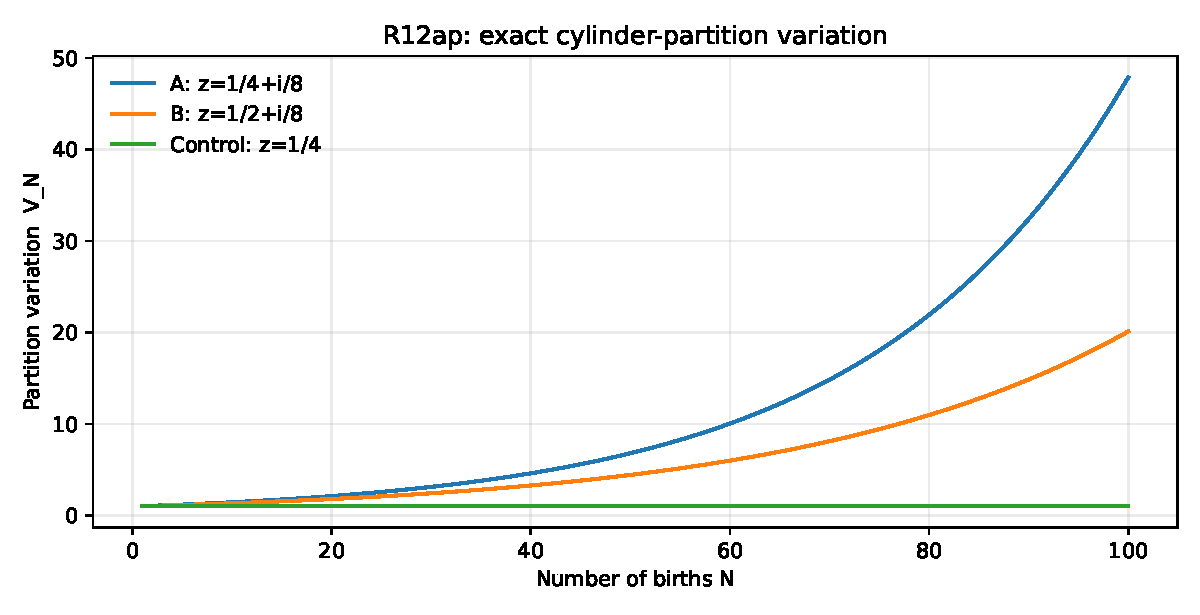
\includegraphics[width=.80\linewidth]{r12ap_total_variation.pdf}
\caption{R12ap: crescita analitica della variazione totale per il partizionamento in relazioni consecutive. Le linee usano l'identita $V_N=b^{N-1}$ senza adattamenti ai dati; il controllo positivo resta a uno.}
\label{fig:r12ap_tv}
\end{figure}

\subsection{Prior art, limiti del gate e decisione}

La mancata estensione di particolari misure quantistiche di crescita causale e un \emph{tema noto}: Dowker--Johnston--Surya hanno analizzato l'estendibilita dei funzionali di decoerenza, mentre Surya--Zalel hanno individuato condizioni in cui classi piu ampie di crescita complessa \emph{ammettono} un'estensione \cite{DowkerJohnstonSurya2010,SuryaZalel2020,Surya2019Review}. Il contributo di R12ap e una prova elementare e un certificato riproducibile \emph{per il ramo scalare e i parametri del nostro progetto}, non una nuova scoperta generale.

La conclusione negativa \emph{non} riguarda automaticamente sotto-algebre covarianti di eventi non etichettati, forme di decoerenza con Hilbert space di dimensione maggiore, operatori QBC non commutativi, ne un eventuale path integral Lorentziano fisico. Nessuna nuova misura 4d selezionata, sorgente energia--impulso con identita di Ward on-shell, risposta retarded, limite continuo o legge cosmologica $H(t)$ e stata ricavata. \textbf{R12ap: FULL LABELLED $\sigma$-EXTENSION FAIL PER $z_A,z_B$; R13 BLOCCATO.} In assenza di un principio microfisico distinto, non e giustificata una successiva serie automatica di varianti della stessa crescita scalare.

\section{Gate R12aq: positivita forte, eventi covarianti ed estensione infinita non selezionano la misura}
\label{sec:r12aq}

\textbf{Domanda e statuto.} R12ap ha escluso l'estensione della particolare percolazione
complessa scalare sulla $\sigma$-algebra completa delle storie naturalmente etichettate.
La conclusione non riguardava l'intera algebra degli osservabili invarianti di un causal
set, ne un generico funzionale di decoerenza. R12aq verifica una condizione piu severa:
\emph{covarianza degli eventi, positivita forte, normalizzazione, consistenza fra
cilindri ed estensione numerabilmente additiva, prese insieme, possono selezionare una
misura quantistica unica?} La risposta e negativa entro un controesempio analitico,
che non introduce alcuna nuova legge della gravita.

\subsection{Teorema astratto di non-selezione}

Sia $(\Omega,\mathcal F,P)$ uno spazio di probabilita. Per parlare di causal set si
consideri la sotto-$\sigma$-algebra degli eventi intrinseci, invarianti sotto
ri-etichettatura naturale, oppure la sua immagine misurabile nello spazio degli ordini
non etichettati. Per ogni $0\le\lambda\le1$ definiamo
\begin{equation}
 \boxed{D_\lambda(A,B)=(1-\lambda)P(A\cap B)+\lambda P(A)P(B),\qquad A,B\in\mathcal F.}
 \label{eq:r12aq_functional}
\end{equation}
Per ogni $\lambda$, $D_\lambda$ e hermitiano, normalizzato, separatamente
numerabilmente additivo e limitato. E \emph{fortemente positivo}: per eventi arbitrari
$A_1,\ldots,A_m$ e coefficienti complessi $c_i$ si ha l'identita
\begin{align}
 \sum_{i,j=1}^m\overline{c_i}D_\lambda(A_i,A_j)c_j
 &=(1-\lambda)\int_\Omega\left|\sum_i c_i\mathbf1_{A_i}\right|^2\,dP\nonumber\\
 &\quad+\lambda\left|\sum_i c_iP(A_i)\right|^2\ge0.
 \label{eq:r12aq_strong_pos}
\end{align}
La consistenza dei cilindri segue dalla restrizione di un unico funzionale globale:
una partizione piu fine si riaggrega per additivita. La covarianza e ereditata
quando $P$ e definita su eventi intrinseci; non e necessario assegnare un'ampiezza a
un'etichetta non osservabile. Inoltre,\emph{ per qualunque evento},
\begin{equation}
 D_\lambda(A,\Omega)=P(A),\qquad
 \mu_\lambda(A):=D_\lambda(A,A)=(1-\lambda)P(A)+\lambda P(A)^2.
 \label{eq:r12aq_same_marginal}
\end{equation}
Dunque perfino \emph{fissare tutti i marginali a una gamba} $D(A,\Omega)$ non
seleziona le interferenze. Le condizioni usate sono quelle standard per il
funzionale di decoerenza e la positivita forte, non un nuovo postulato
microfisico\,\cite{RideoutSorkin2000,DowkerWilkes2020}.

\subsection{Evento intrinseco non banale in crescita causale infinita}

Si usi soltanto come \emph{test logico}, non come teoria 4d, la percolazione
transitiva classica: ciascuna nuova nascita crea indipendentemente un bond con
ciascun elemento precedente, con probabilita $p\in(0,1)$, prima della chiusura
transitiva\,\cite{RideoutSorkin2000}. L'elemento nato dopo $j$ elementi e minimale
se e solo se non possiede bond entranti. Tale evento ha probabilita $(1-p)^j$ ed
e indipendente dagli analoghi eventi delle altre nascite. Pertanto, se
si definisce $E$ come l'evento ``il causal set infinito possiede esattamente un elemento minimale,
\begin{equation}
 \boxed{r(p):=P_p(E)=\prod_{j=1}^{\infty}\bigl[1-(1-p)^j\bigr],\qquad 0<r(p)<1.}
 \label{eq:r12aq_minimal}
\end{equation}
Il prodotto e positivo perche $\sum_{j\ge1}(1-p)^j<\infty$ e nessun fattore
e nullo; e strettamente minore di uno. L'evento $E$ dipende soltanto dall'ordine,
non da una particolare scelta delle etichette. Ponendo $r=r(p)$, la matrice di
decoerenza sulla partizione intrinseca $(E,E^c)$ e
\begin{equation}
 \left.D_\lambda\right|_{E,E^c}=
 \begin{pmatrix}
 (1-\lambda)r+\lambda r^2 & \lambda r(1-r)\\
 \lambda r(1-r) & (1-\lambda)(1-r)+\lambda(1-r)^2
 \end{pmatrix}.
 \label{eq:r12aq_two_event}
\end{equation}
Per la misura quantistica $\mu_\lambda(E)=D_\lambda(E,E)$ e la
interferenza reale fra $E$ ed $E^c$ vale
\begin{equation}
 \boxed{I_\lambda(E,E^c)=\mu_\lambda(\Omega)-\mu_\lambda(E)-\mu_\lambda(E^c)
 =2\lambda r(1-r).}
 \label{eq:r12aq_interference}
\end{equation}
La scelta $\lambda=0$ e diagonale sulle alternative disgiunte e assegna
$\mu_0(E)=r$; la scelta $\lambda=1$ e rank-one, fortemente positiva e
numerabilmente additiva separatamente, ma assegna $\mu_1(E)=r^2$ e
$I_1(E,E^c)>0$. Entrambe hanno $D(E,\Omega)=r$.

\subsection{Controlli esatti e audit indipendente}

Il protocollo e stato congelato in \texttt{R12AQ\_PREREGISTRATION.json} prima
dei calcoli. Per $p=1/2$, la probabilita intrinseca troncata alle prime $N$
nascite e
\begin{equation}
 r_N=\prod_{j=1}^{N-1}\left(1-2^{-j}\right),\quad
 \left|r_\infty-r_{81}\right|\le2^{-80},\quad
 r_\infty=0.288788095086602421\ldots .
 \label{eq:r12aq_numeric_limit}
\end{equation}
La tabella usa esclusivamente frazioni esatte, senza fit:
\begin{table}[htbp]
 \centering\small
 \caption{R12aq: probabilita dell'evento un unico elemento minimale nel
 prefisso e interferenza $I_1=2r_N(1-r_N)$ fra la classe e il complemento.}
 \label{tab:r12aq_finite}
 \begin{tabular}{rll}\toprule
 $N$ & $r_N$ esatto & $I_1(E_N,E_N^c)$ esatto\\\midrule
 2 & $1/2$ & $1/2$\\
 3 & $3/8$ & $15/32$\\
 4 & $21/64$ & $903/2048$\\
 5 & $315/1024$ & $223335/524288$\\
 6 & $9765/32768$ & $224624295/536870912$\\\bottomrule
 \end{tabular}
\end{table}
Il calcolo principale e in aritmetica razionale e ha passato \textbf{3357/3357}
controlli. Un programma indipendente ha enumerato tutti i $2^{N(N-1)/2}$
insiemi di bond, inclusa la chiusura transitiva, con \textbf{70/70} confronti
esatti superati fino a $N=6$. La prima esecuzione del programma principale
si era arrestata per un errore tecnico di indicizzazione, corretto prima di
qualsiasi output valido e registrato in \texttt{R12AQ\_TECHNICAL\_AMENDMENT.md}.
Le verifiche finite di semidefinitezza sono diagnostiche; la dimostrazione
vale per ogni $N$ ed e l'identita~\eqref{eq:r12aq_strong_pos}.

\begin{figure}[htbp]
 \centering
 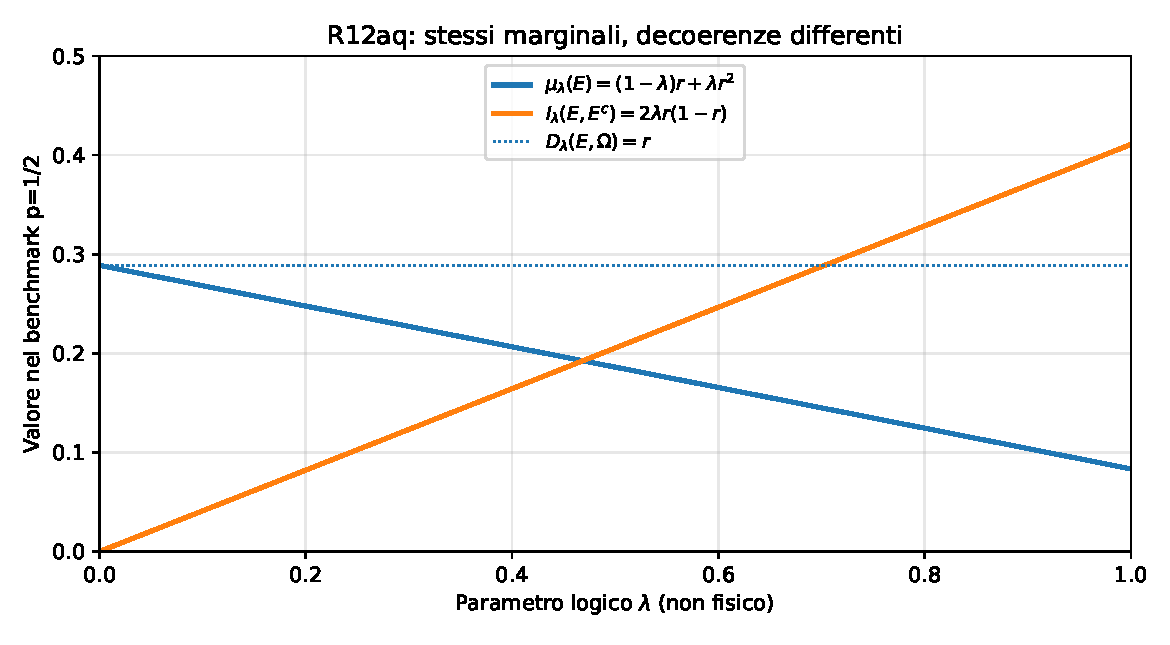
\includegraphics[width=.80\linewidth]{r12aq_covariant_nonuniqueness.pdf}
 \caption{R12aq: cambiando $\lambda$ si modificano misura quantistica
 dell'evento intrinseco e interferenza, mentre tutti i marginali a una gamba
 restano $P(E)=r$. $\lambda$ e un parametro logico del controesempio, non
 un parametro gravitazionale selezionato.}
 \label{fig:r12aq_nonunique}
\end{figure}

\subsection{Verdetto fisico e arresto del ramo parametrico}

Questo risultato e una dimostrazione elementare di \emph{non unicita delle
soluzioni ammissibili} e non risolve la non-estensione della specifica
percolazione complessa scalare R12ap: $D_\lambda$ e una \emph{costruzione
diversa}, basata su una misura classica positiva. Il riferimento a $p$ fisso
continua a ereditare la difficolta geometrica 4d rilevata in R12al. Non sono
derivati da $D_\lambda$ ne l'azione BDG come generatore dinamico, ne la
sorgente gravitazionale con Ward on-shell, ne una risposta retarded, ne il
limite continuo, ne un'equazione autonoma per $H(t)$.

\noindent\textbf{Gate R12aq: STRONG-POSITIVITY/INFINITE-EXTENSION NON-UNIQUENESS
PASS; PHYSICAL DYNAMICS NOT SELECTED; R13 BLOCKED.}
Il teorema non costituisce una priorita scientifica rivendicata: deriva
immediatamente dalle definizioni note di funzionale di decoerenza e dalla
percolazione transitiva classica\,\cite{DowkerWilkes2020,Surya2019Review}.
Un ulteriore gate microfisico richiede un principio \emph{indipendente}
capace di determinare una misura, non una nuova interpolazione parametrica.


\section{Gate R12ar: composizione di sistemi indipendenti, purezza e limite della selezione}

Il Gate R12aq ha dimostrato una non-unicita della misura quantistica su
una algebra di eventi causali intrinseci, pur imponendo forte positivita,
coerenza dei cilindri e additivita numerabile. R12ar affronta un requisito
\emph{aggiuntivo}, motivato dal principio di composizione della teoria
quantistica\,\cite{DowkerWilkes2020}: chiediamo se due sistemi
\emph{matematicamente indipendenti} possano essere descritti dalla stessa
prescrizione globale. Il controllo non postula che due regioni di un unico
universo gravitante siano sistemi tensorialmente indipendenti: la
localizzazione di sottosistemi fisici nella gravita incontra ostacoli di
invarianza di gauge e gravitational dressing\,\cite{DonnellyGiddings2016,DonnellyFreidel2016}.

\subsection{Formula globale e prodotto tensoriale: due operazioni diverse}

Per uno spazio probabilizzato $(\Omega,\mathcal F,P)$ e $0\le\lambda\le1$
richiamiamo il controesempio R12aq
\begin{equation}\label{eq:r12ar_dl}
 D_\lambda(A,B)=(1-\lambda)P(A\cap B)+\lambda P(A)P(B).
\end{equation}
Consideriamo \emph{due copie indipendenti}, $(\Omega_i,\mathcal F_i,P_i)$,
e rettangoli di eventi $A=A_1\times A_2$, $B=B_1\times B_2$.
Definiamo $x_i=P_i(A_i\cap B_i)$ e $y_i=P_i(A_i)P_i(B_i)$.
Applicare la formula~\eqref{eq:r12ar_dl} alla probabilita prodotto
$P_1\otimes P_2$ fornisce
\begin{equation}
 D_\lambda^{\mathrm{glob}}(A,B)=(1-\lambda)x_1x_2+\lambda y_1y_2.
\end{equation}
Comporre invece i \emph{due funzionali locali} fornisce
\begin{equation}
 (D_\lambda^{(1)}\!\otimes D_\lambda^{(2)})(A,B)
 =\big[(1-\lambda)x_1+\lambda y_1\big]
  \big[(1-\lambda)x_2+\lambda y_2\big].
\end{equation}
Sottraendo si ottiene esattamente
\begin{equation}\boxed{\label{eq:r12ar_defect}
 \Delta_\lambda=\lambda(1-\lambda)(x_1-y_1)(x_2-y_2).}
\end{equation}
Per eventi identici e non banali $A_i=B_i=E$ con $P_i(E)=q\in(0,1)$,
\begin{equation}\label{eq:r12ar_simple}
 \Delta_\lambda=\lambda(1-\lambda)q^2(1-q)^2.
\end{equation}
Nell'esempio diagnostico $q=\lambda=1/2$ si ha
$\Delta_\lambda=1/64$. Ne segue che la prescrizione \emph{``applica la
medesima miscela globale con lo stesso $\lambda$''} coincide con il
prodotto dei funzionali locali, per ogni scelta degli eventi, soltanto
agli estremi $\lambda=0$ o $\lambda=1$.

\textbf{Precisione indispensabile:} tale conclusione non e un no-go per
$0<\lambda<1$ contro la composizione in se. Il funzionale
$D_\lambda^{(1)}\otimes D_\lambda^{(2)}$ esiste anche per quei valori ed
e fortemente positivo. Infatti $D_\lambda$ ammette la rappresentazione
come prodotto interno di vettori di evento
\begin{equation}
 v_\lambda(A)=\big(\sqrt{1-\lambda}\,{\bf1}_A,
                    \sqrt\lambda\,P(A)\big)
 \ \in L^2(P)\oplus\mathbb C,
 \qquad D_\lambda(A,B)=\langle v_\lambda(A),v_\lambda(B)\rangle.
\end{equation}
Il prodotto tensoriale conserva la positivita, ma in genere si trova
\emph{fuori} dalla particolare classe di miscele globali a un solo
parametro. Stiamo quindi testando la \emph{chiusura dell'ansatz sotto
composizione}, non l'esistenza di un composto quantistico.

\begin{figure}[htbp]
 \centering
 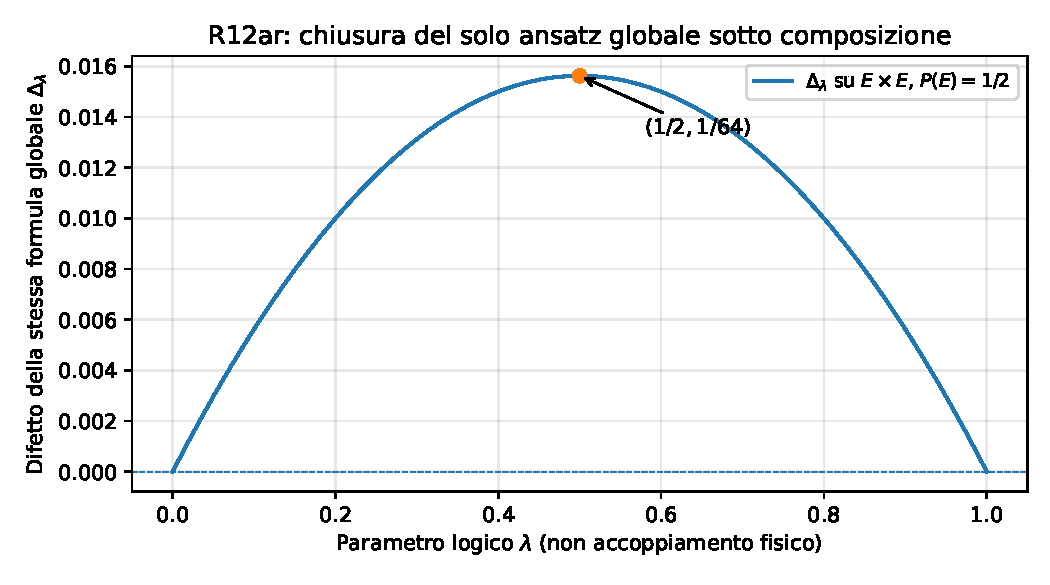
\includegraphics[width=.83\linewidth]{r12ar_composition_defect.pdf}
 \caption{R12ar: difetto di fattorizzazione della \emph{stessa formula
 globale} nel controllo $P(E)=1/2$. Gli estremi $\lambda=0,1$ hanno
 difetto nullo; i valori interni hanno composizione tensoriale positiva
 ma non chiusura entro l'ansatz a parametro globale unico.}
 \label{fig:r12ar_defect}
\end{figure}

\subsection{La purezza restringe $\lambda$, non la probabilita di riferimento}

Per la partizione $(E,E^c)$ con $q=P(E)\in(0,1)$, la matrice di
decoerenza e
\begin{equation}\label{eq:r12ar_matrix}
 M_\lambda=\begin{pmatrix}
 (1-\lambda)q+\lambda q^2 & \lambda q(1-q)\\
 \lambda q(1-q)&(1-\lambda)(1-q)+\lambda(1-q)^2
 \end{pmatrix},
\qquad \det M_\lambda=(1-\lambda)q(1-q).
\end{equation}
Imporre inoltre un funzionale \emph{puro} (rango uno del kernel di
coerenza su una partizione non banale) seleziona $\lambda=1$
\emph{all'interno della famiglia fissata da una data $P$}; per
$0\le\lambda<1$ il rango e due. E un'ipotesi fisica extra,
non una conseguenza degli assiomi del Gate R12aq, ne un teorema di
unicita globale delle misure pure.

\begin{table}[htbp]
 \centering\small
 \caption{R12ar: controlli razionali esatti del difetto nella
 partizione a due eventi; $q$ e una probabilita diagnostica, non
 un parametro cosmologico.}
 \label{tab:r12ar_values}
 \begin{tabular}{cccc}\toprule
 $q$ & $\Delta_0$ & $\Delta_{1/2}$ & $\Delta_1$\\\midrule
 $1/4$ & $0$ & $9/1024$ & $0$\\
 $1/2$ & $0$ & $1/64$ & $0$\\
 $3/4$ & $0$ & $9/1024$ & $0$\\\bottomrule
 \end{tabular}
\end{table}

La selezione di $\lambda=1$ non seleziona ancora $P$. Consideriamo le
due misure di percolazione transitiva classica a parametro \emph{fisso}
$p=1/4$ e $p=3/4$ gia impiegate in R12al. Su ciascuna di esse la
costruzione pura $D_1^{(p)}(A,B)=P_p(A)P_p(B)$ e fortemente positiva,
normalizzata, additiva e fattorizzante per \emph{due copie indipendenti}.
Sull'evento causale intrinseco $E$ ``il causet infinito ha esattamente
un elemento minimale'' si ha
\begin{equation}
 P_p(E)=r(p)=\prod_{j=1}^{\infty}\left[1-(1-p)^j\right],
 \qquad 0<r(1/4)<r(3/4)<1.
\end{equation}
La disuguaglianza e rigorosa poiche ogni fattore del prodotto e
strettamente crescente in $p$. Quindi le due misure pure differiscono
\emph{sullo stesso osservabile non etichettato}. I due valori $p$ sono
esempi logici fissati a priori, non parametri adattati alla cosmologia.
Inoltre la percolazione a $p$ fissato non supera il benchmark geometrico
4d di R12al; questo resta un \emph{controesempio alla selezione}, non
una dinamica gravitazionale accettabile.

\subsection{Verifiche, limiti e decisione fisica}

Il protocollo \texttt{R12AR\_PREREGISTRATION.json} e stato congelato
prima dei risultati. I controlli simbolici ed esatti hanno prodotto
\textbf{46/46 PASS}; un secondo calcolatore, basato su aritmetica
\texttt{Fraction} ed eventi enumerati, ha prodotto \textbf{2466/2466
PASS}. La prima esecuzione del codice principale si era fermata per
una conversione non valida di autovalori algebrici a numeri razionali;
la verifica e stata corretta in minori principali esatti senza cambiare
il test, e l'emendamento e conservato nell'audit. Nessuna osservazione
cosmologica e stata usata.

\textbf{Verdetto R12ar:} i requisiti aggiuntivi di composizione e di
purezza possono restringere una famiglia matematica, ma non selezionano
la misura di riferimento, il peso BDG 4d come dinamica, una sorgente
Ward/Bianchi conservata on-shell, la relazione tra rumore e risposta
retarded, o un limite continuo. E improprio attribuire automaticamente
un prodotto tensoriale a due regioni fisiche di gravita quantistica.
\begin{center}\small
 \nolinkurl{R12AR_COMPOSITION_PURITY_RESTRICTIONS_PASS_PHYSICAL_SELECTION_BLOCKER_PERSISTS_R13_BLOCKED}
\end{center}
Un ulteriore gate microdinamico richiede un \emph{nuovo principio
indipendente} che specifichi quegli ingredienti; non viene autorizzata
una prosecuzione parametrica automatica. \textbf{R13 resta BLOCCATO.}


\section{Checkpoint di fattibilita R12as: selezione microdinamica, Ward e risposta}
\label{sec:r12as-screen}

\textbf{Status del checkpoint: \status{SCREENING ESEGUITO; R12as FISICO NON AUTORIZZATO; R13 BLOCCATO}.}
Il checkpoint non introduce un'altra famiglia parametrica di funzioni di decoerenza.
La domanda, imposta dai Gate R12ai--R12ar, e se esista un \emph{unico candidato fisico
indipendentemente motivato} che colleghi sul medesimo spazio di storie: misura
quantistica, azione gravitazionale, conservazione dinamica, rumore e risposta
retarded e limite continuo quadridimensionale. L'evidenza consultata non
identifica ancora un tale candidato completo. Questo e un giudizio sul materiale
verificato, \emph{non} una dimostrazione che nessun programma futuro possa riuscirci.

\subsection{Tre programmi indipendenti e requisiti non intercambiabili}

Il programma della \emph{quantum sequential growth} (QSG) mantiene il causal
order come struttura primaria. Il recente lavoro di Srivastava e Surya
\cite{SrivastavaSurya2026} impone versioni della quantum Bell causality agli
operatori di transizione: alcune prescrizioni inducono commutativita; una
terza conserva vincoli operatoriali non banali ma non ricava una formula
generale calcolabile delle transizioni. Non sono percio disponibili da quel
risultato, gia da solo, la sorgente gravitazionale on-shell e un limite
cosmologico 4d. L'ostacolo storico alla selezione della misura QSG e discusso
anche nella review di Surya \cite{Surya2019Review}.

Le \emph{causal dynamical triangulations} (CDT) 4d realizzano invece una
regolarizzazione a somma su geometrie di una teoria gravitazionale diversa
dai causal set come poset. Nella fase semiclassica di de Sitter e stata
ricostruita una dinamica efficace del fattore di scala, mentre il limite
ultravioletto e oggetto di studio \cite{GizbertStudnicki2024,Loll2019CDT}.
Questi risultati costituiscono un confronto positivo importante, ma non
selezionano automaticamente una misura QSG o il rumore tensoriale causale
specifico di questo quaderno.

La \emph{gravita stocastica} basata sul formalismo Schwinger--Keldysh/
closed-time-path (CTP) parte da campi quantistici su una metrica continua e
deriva una sorgente con conservazione covariante, un noise kernel positivo
e una risposta retarded mediante la stessa dinamica di materia
\cite{HuVerdaguer2008}. Essa costituisce il controllo fisico piu vicino ai
requisiti di Ward e rumore--risposta, ma \emph{non} seleziona la somma
quantistica su causal set ne la dinamica geometrica di $H(t)$.

\begin{table}[htbp]
\centering\small
\caption{R12as: audit di compatibilita, \emph{non} assegnazione di un nuovo modello. Un controllo positivo in una teoria non viene trasferito automaticamente a un'altra.}
\begin{tabular}{p{0.19\linewidth}p{0.34\linewidth}p{0.35\linewidth}}
\toprule
Programma & Ingrediente effettivamente disponibile & Ingrediente ancora non derivato per il progetto \\
\midrule
QSG / causal set & Ordini causali, ipotesi sulla crescita e vincoli operatoriali di causalita quantistica & Misura fisica unica, fonte Ward 4d, rumore--risposta e limite cosmologico \\
CDT 4d & Somma regolata su triangolazioni causali, fase semiclassica con geometria estesa & Identificazione con la dinamica quantistica dei poset e sorgente stocastica del modello di overlap \\
CTP / gravita stocastica & Funzionale in-in continuo, stress on-shell conservato, noise kernel e risposta causale & Origine di una misura gravitazionale QSG e ricostruzione microdinamica del settore di vuoto \\
\bottomrule
\end{tabular}
\end{table}

\subsection{Controllo costruttivo indipendente: l'identita di Ward non seleziona la dinamica}

Per un campo scalare reale omogeneo su FLRW piatta, con segnatura $(-,+,+,+)$
e in unita naturali, scegliamo il benchmark \emph{noto}
\begin{equation}
S_{\mathrm m}[g,\phi]=\int d^4x\sqrt{-g}\,
\left[-\frac12 g^{\mu\nu}\partial_\mu\phi\partial_\nu\phi
 -V(\phi)\right].
\end{equation}
Definendo $E_\phi=\Box\phi-V'(\phi)$ e il tensore
$T_{\mu\nu}=-2\,\delta S_{\rm m}/(\sqrt{-g}\,\delta g^{\mu\nu})$,
l'invarianza per diffeomorfismi fornisce l'identita on-shell
\begin{equation}
\nabla_\mu T^{\mu}{}_{\nu}=E_\phi\,\nabla_\nu\phi,
\qquad \nabla_\mu T^{\mu}{}_{\nu}=0\quad\text{se } E_\phi=0.
\end{equation}
Per $\phi=\phi(t)$ si ottiene
\begin{equation}
\rho_\phi=\tfrac12\dot\phi^2+V(\phi),\qquad
p_\phi=\tfrac12\dot\phi^2-V(\phi),\qquad
E_\phi=-\ddot\phi-3H\dot\phi-V'(\phi),
\end{equation}
quindi
\begin{equation}
\boxed{\dot\rho_\phi+3H(\rho_\phi+p_\phi)
=\dot\phi\bigl(\ddot\phi+3H\dot\phi+V'(\phi)\bigr)
=-E_\phi\dot\phi.}
\end{equation}
Questo passaggio e stato verificato \emph{due volte}, prima simbolicamente
con un potenziale generico e poi con i simboli di Christoffel e la divergenza
di $T^{\mu}{}_{\nu}$ calcolati direttamente: 6/6 e 7/7 controlli PASS.
Anche $V=0$ e $V=m^2\phi^2/2$ soddisfano la stessa identita di Ward,
ma hanno equazioni di moto differenti. La conservazione \emph{non seleziona}
$V$, il path sum gravitazionale o la legge dell'espansione. I programmi
riproducibili accompagnano il recovery; non e stata effettuata alcuna
simulazione cosmologica e non vi sono parametri calibrati sui dati.

\subsection{Perche rumore e risposta richiedono una microfisica comune}

Nel benchmark CTP con un vero operatore energia--impulso $\hat T_{\mu\nu}$,
posto $\hat t=\hat T-\langle\hat T\rangle$, il noise kernel e
\begin{equation}
N_{\mu\nu\rho\sigma}(x,y)=\tfrac12
\big\langle\{\hat t_{\mu\nu}(x),\hat t_{\rho\sigma}(y)\}\big\rangle.
\end{equation}
Per funzioni test reali simmetriche $f^{\mu\nu}$, se
$X_f=\int d\mu\,f^{\mu\nu}\hat t_{\mu\nu}$ e autoaggiunto,
\begin{equation}
\int d\mu_x d\mu_y\,f^{\mu\nu}(x)
N_{\mu\nu\rho\sigma}(x,y)f^{\rho\sigma}(y)
=\langle X_f^2\rangle\ge0.
\end{equation}
La risposta causale e legata al commutatore ritardato
\begin{equation}
R^{\mathrm{ret}}_{\mu\nu\rho\sigma}(x,y)
\propto i\,\Theta(t_x-t_y)
\langle[\hat T_{\mu\nu}(x),\hat T_{\rho\sigma}(y)]\rangle,
\end{equation}
con i necessari termini locali di contatto/variazione della metrica.
In una teoria definita, conservazione e condizioni al bordo seguono dai
campi dinamici, dallo stato e dall'azione. \emph{Non} e lecito copiare il
kernel di sovrapposizione scalare R12g nel posto di $N$, postulare una
risposta $R^{\mathrm{ret}}$ indipendente e chiamare il risultato una chiusura
quantistica: verrebbero introdotti nuovi input fisici non selezionati.

\subsection{Verdetto del checkpoint: soglia esplicita per autorizzare R12as}

Un futuro R12as fisico e autorizzabile solo se viene esibito un \emph{singolo}
modello con (i) storie 4d e simmetrie di rietichettatura/covarianza,
(ii) misura quantistica e azione che producano una dinamica controllabile,
(iii) sorgente gravitazionale conservata on-shell per Ward/Bianchi,
(iv) rumore positivo e risposta retarded derivati dal medesimo generatore,
(v) coarse-graining e limite 4d verificabili. Il comportamento $H(z)$ non
puo essere utilizzato per determinare gli ingredienti da derivare.
\textbf{Alla data del checkpoint, nessuno dei candidati esaminati supera
simultaneamente questi cinque requisiti nel quadro CC\_CAUSAL\_EXPANSION.}
Non si tratta di un nuovo \emph{no-go} universale, ma di un esito
\emph{fail-closed} di fattibilita. Il \textbf{Gate R12as non e stato aperto come
test di nuova microdinamica}; \textbf{R13 resta BLOCCATO}.

\begin{center}\small
\nolinkurl{R12AS_PRE_GATE_SCREEN_PASS_WARD_POSITIVE_CONTROL_PASS_PHYSICAL_SELECTION_BLOCKER_PERSISTS_R13_BLOCKED}
\end{center}

\section{Screening R12at: operatore retarded 4d e ostacolo variazionale a campo singolo}
\label{sec:r12at-screen}

\textbf{Status: \status{SCREENING ANALITICO PASS; MICRODINAMICA FISICA NON SELEZIONATA; R13 BLOCCATO}.}
Questo controllo non apre il Gate fisico R12as, che richiede ancora una misura quantistica
sulle geometrie 4d, un generatore di sorgente Ward/Bianchi, rumore e risposta dalla stessa
microfisica e un limite continuo verificato. Non sono stati adattati parametri o utilizzati
osservabili cosmologici come input. Si sottopone invece a verifica una condizione necessaria
per un candidato costruito a partire da un operatore causale discreto noto.

\subsection{Operatore retarded di Benincasa--Dowker in quattro dimensioni}
Un causal set finito e un ordine parziale localmente finito. Scegliamo una estensione lineare
nella quale $j\prec i$ implica $j<i$. La forma standard, adimensionale, dell'operatore
scalare a quattro dimensioni \cite{Surya2019Review,BenincasaDowker2010} e
\begin{equation}
 \widetilde B_{ij}=-\delta_{ij}+
 \begin{cases}
  b_{k(j,i)}, & j\prec i,\quad k(j,i)\in\{0,1,2,3\},\\
  0, & \text{altrimenti},
 \end{cases}
 \qquad (b_0,b_1,b_2,b_3)=(1,-9,16,-8).
 \label{eq:r12at_B}
\end{equation}
Qui $k(j,i)$ e il numero di elementi \emph{strettamente compresi} nell'intervallo causale
$(j,i)$. Il prefattore fisico usuale e $4/(\sqrt6\,\ell^2)$, omesso nelle verifiche intere,
poiche non influisce sulla simmetria. L'operatore e retarded nel senso algebrico che
$(\widetilde B\phi)_i$ usa soltanto $\phi_i$ e valori $\phi_j$ nel passato causale di $i$.
Nelle condizioni di sprinkling e smearing studiate nella letteratura, il limite medio
opportunamente riscalato e legato a $(\Box-R/2)\phi$; il presente controllo \emph{non}
calcola tale limite, ne dimostra stabilita dell'evoluzione o emergenza di un manifold 4d.

\subsection{Lemma di Helmholtz finito: l'azione quadratica non conserva il retarded}
Per un campo scalare reale $\phi\in\mathbb R^n$ consideriamo
\begin{equation}
 S_1[\phi]=\frac12\,\phi^{\mathsf T}\widetilde B\phi.
\end{equation}
La sua equazione di Eulero--Lagrange, variando tutte le componenti, e
\begin{equation}
 \frac{\partial S_1}{\partial\phi}
 =\underbrace{\frac{\widetilde B+\widetilde B^{\mathsf T}}2}_{\displaystyle H}\phi,
 \qquad H=H^{\mathsf T}. \label{eq:r12at_H}
\end{equation}
In modo piu generale, se una qualunque funzione $S\in C^2(\mathbb R^n)$
avesse gradiente $\nabla S(\phi)=\widetilde B\phi$ per \emph{ogni} $\phi$,
le derivate miste imporrebbero $\widetilde B_{ij}=\widetilde B_{ji}$.
Ogni ordine con almeno una relazione possiede almeno un \emph{cover link}, e il suo
coefficiente retarded vale $b_0=1$: non avendo un coefficiente nel futuro
corrispondente, $\widetilde B$ non e simmetrico. Ne segue un no-go \emph{ristretto}:
non si ottiene $\widetilde B\phi=0$ dalla variazione di una normale azione
reale a \emph{campo singolo} con gradiente lineare $\widetilde B\phi$.
Una pesatura positiva diagonale $W$ non risolve l'ostacolo:
$\nabla(\phi^{\mathsf T}W\widetilde B\phi/2)
=(W\widetilde B+\widetilde B^{\mathsf T}W)\phi/2$.

Per una catena di tre elementi, l'esempio intero esatto e
\begin{equation}
 \widetilde B=\begin{pmatrix}-1&0&0\\1&-1&0\\-9&1&-1\end{pmatrix},\qquad
 H=\begin{pmatrix}-1&1/2&-9/2\\1/2&-1&1/2\\-9/2&1/2&-1\end{pmatrix}.
\end{equation}
Il secondo operatore introduce coefficienti che collegano una riga anche al futuro.
\begin{figure}[htbp]
\centering
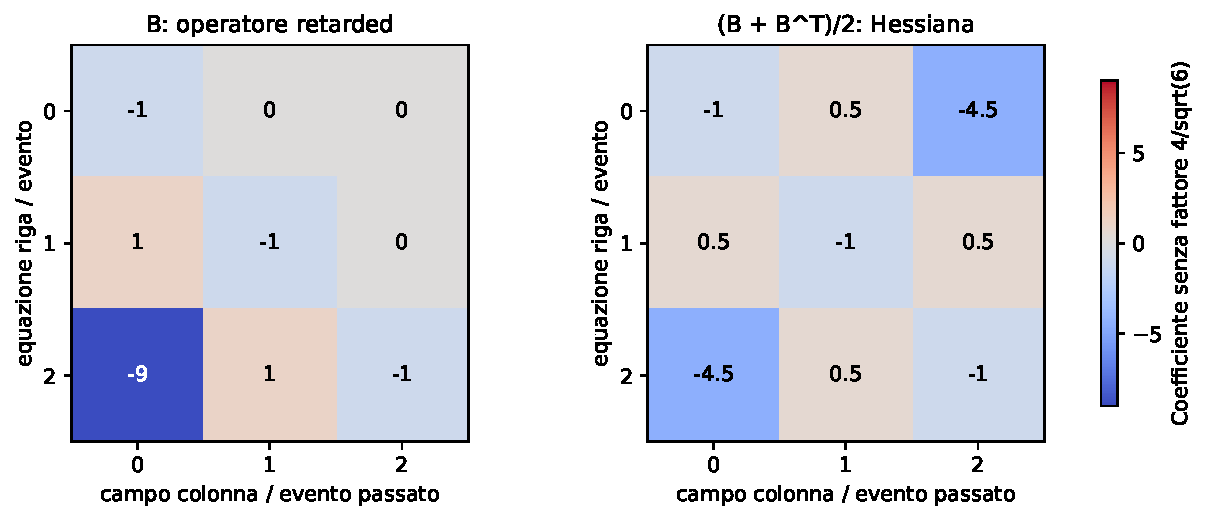
\includegraphics[width=0.94\linewidth]{r12at_retarded_vs_hessian.pdf}
\caption{Catena a tre elementi: il kernel retarded e triangolare; la Hessiana
simmetrica dell'azione a campo singolo introduce anche i contributi trasposti.
Coefficienti esatti, non provenienti da un fit.}
\label{fig:r12at-matrices}
\end{figure}

\subsection{Rimedio algebrico a due rami e nuova non unicita}
Come test \emph{formale}, non come influenza funzionale quantistica derivata,
introduciamo $\phi_r$ (campo medio) e $\phi_a$ (campo di risposta) e
\begin{equation}
 \Gamma_N[\phi_r,\phi_a]=
 \phi_a^{\mathsf T}\widetilde B\phi_r
 +\frac{i}{2}\phi_a^{\mathsf T}N\phi_a,
 \qquad N=N^{\mathsf T}\succeq0. \label{eq:r12at_ctp}
\end{equation}
Per campi reali si verificano \emph{esattamente} le identita
\begin{align}
 \Gamma_N[\phi_r,0]&=0,\\
 \Gamma_N[\phi_r,\phi_a]^*&=-\Gamma_N[\phi_r,-\phi_a],\\
 \left.\frac{\partial\Gamma_N}{\partial\phi_a}\right|_{\phi_a=0}
 &=\widetilde B\phi_r,\qquad
 \operatorname{Im}\Gamma_N=\tfrac12\phi_a^{\mathsf T}N\phi_a\ge0.
\end{align}
Il retarded compare come equazione ottenuta variando il campo di risposta;
non si tratta piu della variazione di una azione quadratica ordinaria per un solo campo.
Tuttavia la stessa $\widetilde B$ e compatibile algebricamente con
$N=I$ e con $N=\mathrm{diag}(1,2,\ldots,n)$, entrambe positive e diverse:
\emph{la risposta non determina la statistica delle fluttuazioni}.
Queste condizioni non garantiscono da sole un reale funzionale CTP unitario,
una matrice densita positiva o una corretta relazione fluctuation--dissipation:
per questo rumore e risposta dovrebbero derivare dal \emph{medesimo} modello
microscopico, come nel benchmark di gravita stocastica \cite{HuVerdaguer2008}.

\subsection{Validazione finita e limiti}
La preregistrazione ha fissato coefficienti, sample space, test simbolici e criteri
prima dei calcoli. Il programma principale ha enumerato \emph{tutti} gli ordini
naturalmente etichettati distinti ottenuti con chiusura transitiva per $n=2,\ldots,6$:
\begin{center}
\begin{tabular}{r r r r}
\toprule
$n$ & Ordini distinti & Non-antichain non simmetrici & Antichain \\
\midrule
2 & 2 & 1 & 1\\
3 & 7 & 6 & 1\\
4 & 40 & 39 & 1\\
5 & 357 & 356 & 1\\
6 & 4824 & 4823 & 1\\
\midrule
Totale & 5230 & 5225 & 5\\
\bottomrule
\end{tabular}
\end{center}
L'implementazione indipendente usa una diversa enumerazione degli archi e
la chiusura Floyd--Warshall: l'insieme delle relazioni coincide bit per bit
fino a $n=5$; sono verificate anche cinque fixture a sei elementi.
Una prima run diagnostica del programma principale ha intercettato un errore
\emph{di orientamento} nel termine bilineare a due campi ($\phi_r^{\mathsf T}
\widetilde B\phi_a$ invece di $\phi_a^{\mathsf T}\widetilde B\phi_r$):
corretto prima del replay valido e registrato in 
\texttt{R12AT\_TECHNICAL\_AMENDMENT.md}; non e un PASS retroattivo.
A livello finito $\widetilde B$ e triangolare con diagonale $-1$, quindi
$\det\widetilde B=(-1)^n$: l'equazione omogenea su \emph{tutti} gli elementi
senza dati al bordo impone $\phi=0$. Un problema fisico non banale necessita
di sorgenti, condizioni iniziali o prescrizioni di bordo adeguate; nemmeno
questi dati sono selezionati dai semplici assiomi cinematici.

\subsection{Decisione fisica R12at}
\textbf{PASS algebrico:} l'ostacolo variazionale e dimostrato per la classe
monocampo, e un raddoppio CTP retarded e matematicamente costruibile.
\textbf{Non derivati:} misura quantistica della geometria, noise kernel dalla
microfisica, Ward/Bianchi gravitazionali, stabilita o continuum 4d e
predizione indipendente di $H(t)$. I risultati sono applicazioni di algebra
finita a un operatore gia noto, \emph{non un no-go sulla gravita quantistica}.
\textbf{R12as fisico ancora NON AUTORIZZATO; R13 BLOCCATO.}
\begin{center}\small
\nolinkurl{R12AT_PRE_GATE_VARIATIONAL_OBSTRUCTION_PASS_DOUBLED_RESPONSE_ALGEBRA_PASS_NOISE_AND_GRAVITY_SELECTION_BLOCKED_R13_BLOCKED}
\end{center}


\clearpage
\section{Screening R12au: risposta e fluttuazioni dalla stessa microfisica quantistica}
\label{sec:r12au-screen}
\textbf{Classificazione: \status{CONTROLLO MICROFISICO POSITIVO SU SFONDO FISSO; SELEZIONE DELLO STATO E GRAVITA DINAMICA NON DERIVATE}.}
R12at aveva mostrato che una costruzione a due rami puo mantenere una risposta retarded, ma non determina il rumore se questo viene introdotto come matrice semidefinita positiva arbitraria. R12au verifica una condizione piu forte: \emph{esistenza di una singola microdinamica quantistica dalla quale calcolare entrambi i kernel}. Il modello e un controllo positivo noto, non una proposta gravitazionale originale e neppure un nuovo Gate R12as fisico. Nessun parametro viene scelto per riprodurre $H(t)$ o osservazioni cosmologiche.

\subsection{Un campo libero in $3+1$ dimensioni, geometria non dinamica}
In un toro spaziale di lato $2\pi$ con metrica di Minkowski prefissata $\eta_{\mu\nu}=\mathrm{diag}(-1,1,1,1)$, usiamo $c=\hbar=1$ e il campo reale libero di massa $m=1$:
\begin{equation}
 S_{\mathrm m}[\varphi]=-\frac12\int d^4x\,\bigl(\partial_\mu\varphi\,\partial^\mu\varphi+\varphi^2\bigr),
 \qquad (\Box-1)\varphi=0.
 \label{eq:r12au_field}
\end{equation}
Ciascun modo reale opportunamente normalizzato soddisfa $\ddot q_{\mathbf k}+\omega_{\mathbf k}^2q_{\mathbf k}=0$, con $\omega_{\mathbf k}=\sqrt{1+|\mathbf k|^2}$ e Hamiltoniana
\begin{equation}
 H_{\mathbf k}=\frac12\bigl(p_{\mathbf k}^2+\omega_{\mathbf k}^2q_{\mathbf k}^2\bigr),
 \qquad [q_{\mathbf k},p_{\mathbf k}]=i.
 \label{eq:r12au_ham}
\end{equation}
La decomposizione modale serve a eseguire controlli esatti e non trasforma il background di Minkowski in una geometria da sommare quantisticamente. Il formalismo in-in e la derivazione dei kernel di rumore da correlatori sono ben noti in teoria dei sistemi aperti e gravita stocastica \cite{FeynmanVernon1963,HuVerdaguer2008}.

\subsection{Un unico operatore quantistico determina due kernel}
Per lo stesso modo con $\omega>0$ e per uno stato termico di Gibbs $\rho_\beta\propto e^{-\beta H}$, l'evoluzione di Heisenberg implica
\begin{equation}
 q(t)=q(0)\cos(\omega t)+\frac{p(0)}{\omega}\sin(\omega t),\qquad
 [q(t),q(s)]=-\frac{i}{\omega}\sin\bigl(\omega(t-s)\bigr).
 \label{eq:r12au_comm}
\end{equation}
Usando la convenzione $G_R(t,s)=i\Theta(t-s)\langle[q(t),q(s)]\rangle$ e il correlatore simmetrizzato connesso $N_\beta(t,s)=\frac12\langle\{\Delta q(t),\Delta q(s)\}\rangle_\beta$, si trova esattamente
\begin{align}
 G_R(t,s)&=\Theta(t-s)\frac{\sin\bigl(\omega(t-s)\bigr)}{\omega},
 \label{eq:r12au_retarded}\\
 N_\beta(t,s)&=\frac{2n_\beta+1}{2\omega}\cos\bigl(\omega(t-s)\bigr),
 \qquad n_\beta=\frac{1}{e^{\beta\omega}-1}.
 \label{eq:r12au_noise}
\end{align}
Lo spettro di rumore soddisfa la relazione termica di fluttuazione--dissipazione con il corrispondente commutatore; la temperatura, tuttavia, e un dato di stato, non una conseguenza della sola equazione ritardata. La positivita del kernel e immediata: per qualunque insieme finito di tempi $t_i$ e coefficienti reali $v_i$,
\begin{equation}
 \sum_{ij}v_i N_\beta(t_i,t_j)v_j
 =\frac{2n_\beta+1}{2\omega}\left|\sum_i v_i e^{i\omega t_i}\right|^2\geq0.
 \label{eq:r12au_psd}
\end{equation}
Quindi la matrice di covarianza e semidefinita positiva \emph{per costruzione dal medesimo stato e Hamiltoniana}, e non perche una matrice $N$ sia stata scelta dopo aver fissato la risposta.

\subsection{Controesempio esatto alla selezione del rumore dalla sola risposta}
Manteniamo \emph{identici} $H$ e $G_R$ e confrontiamo il vuoto ($\beta\to\infty$) con uno stato termico $\beta=\ln3$, scelta di controllo aritmetico e non adattamento fenomenologico. Per il modo $\omega_0=1$,
\begin{equation}
 n_{\infty}=0,\quad n_{\ln3}=\frac12,\qquad
 N_{\infty}(t,s)=\frac12\cos(t-s),\quad
 N_{\ln3}(t,s)=\cos(t-s)=2N_{\infty}(t,s).
 \label{eq:r12au_double}
\end{equation}
La risposta retarded e invece $G_R(t,s)=\Theta(t-s)\sin(t-s)$ in \emph{entrambi} gli stati. Il confronto non e un no-go per una teoria che \emph{specifichi} il proprio stato iniziale: dimostra precisamente che il solo dato di risposta, perfino se proviene da una Hamiltoniana quantistica completa, non seleziona il correlatore simmetrizzato senza una condizione sullo stato.

\begin{figure}[htbp]
 \centering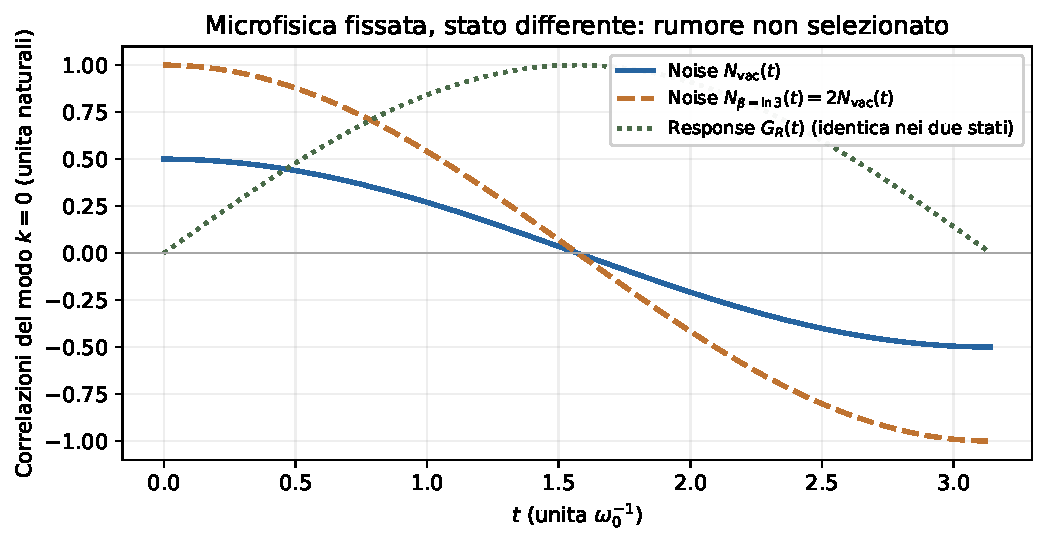
\includegraphics[width=0.82\textwidth]{r12au_state_noise.pdf}
 \caption{Benchmark microfisico a sfondo fisso, modo $\omega=1$. La risposta causale non cambia passando dal vuoto allo stato termico, mentre la covarianza simmetrizzata raddoppia. Le curve sono formule analitiche, non fit.}
 \label{fig:r12au-state}
\end{figure}

\subsection{Unitarieta in-in e identita di conservazione: cosa controllano davvero}
Per sorgenti esterne reali $J_+,J_-$, la definizione operatoriale del funzionale a tempo chiuso e
\begin{equation}
 Z[J_+,J_-]=\mathrm{Tr}\bigl(U_{J_+}\rho_\beta U_{J_-}^{\dagger}\bigr),
 \qquad Z[J,J]=\mathrm{Tr}\rho_\beta=1,
 \label{eq:r12au_ctp}
\end{equation}
per unitarieta dell'evoluzione in ciascuna storia di sorgente. La conservazione classica dell'energia--impulso del campo libero segue \emph{on-shell} dalla identita
\begin{equation}
 T_{\mu\nu}=\partial_\mu\varphi\partial_\nu\varphi-\eta_{\mu\nu}\left[\frac12\partial_\alpha\varphi\partial^\alpha\varphi+\frac12\varphi^2\right],\qquad
 \partial^\mu T_{\mu\nu}=(\Box\varphi-\varphi)\partial_\nu\varphi.
 \label{eq:r12au_ward}
\end{equation}
Questa verifica \emph{non} include rinormalizzazione dell'operatore composito $\widehat T_{\mu\nu}$, il suo noise kernel tensoriale, le identita di Ward gravitazionali quantistiche su geometrie dinamiche o la conservazione di una sorgente di Einstein--Langevin generata da causal set. E una identita classica di una materia con azione specificata su sfondo fisso.

\subsection{Protocollo congelato, controlli e limiti}
Il protocollo $\texttt{R12AU\_PREREGISTRATION.json}$ e stato scritto e sottoposto a SHA-256 prima di eseguire i due programmi. I nove controlli primari comprendono le formule simboliche, lo stato termico, la positivita su 25 tempi per i tre modi $|\mathbf k|=0,1,2$ e l'identita di conservazione per le quattro componenti. Il programma indipendente usa una rappresentazione di Fock a dimensione 32, calcola le tracce degli operatori per tre separazioni temporali e verifica $Z[J,J]$ con tre sorgenti predeterminate, per entrambi gli stati.
\begin{center}
\begin{tabular}{p{0.57\textwidth}rr}
\toprule
Controllo & Risultato & Stato\\
\midrule
Formule e identita simboliche primarie & $9/9$ & PASS\\
Tracce Fock, CTP e positivita indipendenti & $23/23$ & PASS\\
Identita $N_{\ln3}=2N_{\infty}$ per $\omega_0=1$ & Esatta & PASS\\
Retarded uguale per i due stati & Esatta & PASS\\
Selezione di stato, misura grav. 4d e continuum & --- & NON DERIVATI\\
\bottomrule
\end{tabular}
\end{center}
Nell'integrazione numerica il piu piccolo autovalore calcolato nelle matrici di rumore e dell'ordine di $-10^{-15}$, coerente con l'arrotondamento; la dimostrazione \eqref{eq:r12au_psd} non si basa su questa soglia. I risultati numerici non costituiscono una stima di osservabili cosmologici.

\subsection{Decisione scientifica R12au}
\textbf{Superato il controllo microfisico di consistenza:} esiste una teoria quantistica ordinaria in 4d (campo libero su Minkowski \emph{fisso}) che fornisce risposta retarded e rumore dalla stessa azione e dallo stato scelto, con positivita e consistenza unitaria. \textbf{Non superato il gate gravitazionale:} lo stato iniziale non e selezionato dalla risposta, la misura quantistica su geometrie causal-set 4d non e stata definita, non esiste una sorgente gravitazionale tensoriale dinamica derivata in questo controllo e non e stato provato il limite continuo gravitazionale. La classe gia nota delle azioni e influenze quantistiche soddisfa dunque una parte dei requisiti ma non produce una chiusura cosmologica autonoma. \textbf{R12as fisico NON AUTORIZZATO; R13 BLOCCATO.}
\begin{center}\small
\nolinkurl{R12AU_MICROPHYSICAL_FREE_FIELD_BENCHMARK_PASS_STATE_AND_GRAVITY_SELECTION_BLOCKED_R13_BLOCKED}
\end{center}

\clearpage
\section{Screening R12av: noise tensoriale di energia--impulso da una microfisica fissata}
\label{sec:r12av-stress}
\textbf{Classificazione: \status{BENCHMARK DI MATERIA 4D A MODI FINITI: PASS; GRAVITA DINAMICA NON DERIVATA}.}

La v0.51 (R12au) aveva calcolato il rumore \emph{del campo} libero e la sua risposta retarded; non aveva costruito il correlatore dell'operatore energia--impulso. R12av affronta esattamente questa lacuna, ma soltanto in una teoria di materia quantistica \emph{su metrica prefissata}. La definizione corretta del noise tensoriale nella gravita stocastica e il correlatore anticommutatore connesso di due tensori energia--impulso \cite{HuVerdaguer2008,PhillipsHu2001}. Non viene proposto un nuovo operatore della gravita quantistica.

\subsection{Modello congelato, stato e tensore canonico}
Assumiamo lo stesso campo scalare reale libero di massa $m=1$, $c=\hbar=1$, sullo spazio-tempo $\mathbb R\times\mathbb T^3$ di lato spaziale $L=2\pi$, con $\eta_{\mu\nu}=\mathrm{diag}(-1,1,1,1)$. Prima della produzione si e congelato un \emph{cutoff finito} di sette modi reali ortonormali:
\begin{equation}
 f_0=V^{-1/2},\qquad f_{i,c}=\sqrt{2/V}\cos x_i,\qquad
 f_{i,s}=\sqrt{2/V}\sin x_i\quad (i=1,2,3),\quad V=L^3.
 \label{eq:r12av-modes}
\end{equation}
Ogni modo ha frequenza $\omega_a=\sqrt{1+|\mathbf k_a|^2}$. Il campo troncato
\begin{equation}
 \hat\phi(t,\mathbf x)=\sum_a f_a(\mathbf x)
 \left[\hat q_a\cos(\omega_at)+\frac{\hat p_a}{\omega_a}\sin(\omega_at)\right]
 \label{eq:r12av-field}
\end{equation}
soddisfa esattamente $(\Box-1)\hat\phi=0$ come identita operatoriale \emph{a cutoff finito}, e $[\hat q_a,\hat p_b]=i\delta_{ab}$. Consideriamo lo stato fondamentale dell'Hamiltoniana libera e lo stato di Gibbs alla temperatura assegnata $\beta^{-1}$, con $\beta=\ln3$ soltanto come controllo. Nello spazio delle variabili canoniche $Z=(q_0,p_0,\ldots)$ poniamo
\begin{equation}
\begin{aligned}
 V_{AB}&=\frac12\langle\{\Delta Z_A,\Delta Z_B\}\rangle,\qquad
 [Z_A,Z_B]=iJ_{AB},\\
 V_a&=\begin{pmatrix}\nu_a/\omega_a&0\\0&\nu_a\omega_a\end{pmatrix},
 \qquad \nu_a=n_a+\frac12,\quad n_a=(e^{\beta\omega_a}-1)^{-1}.
\end{aligned}
 \label{eq:r12av-canonical-cov}
\end{equation}
con $n_a=0$ nel vuoto. Si tratta di dati di stato: non sono selezionati dalla causalita del background.

Il tensore energia--impulso canonico minimo e
\begin{equation}
 \hat T_{\mu\nu}=\frac12\{\partial_\mu\hat\phi,\partial_\nu\hat\phi\}
 -\frac12\eta_{\mu\nu}\bigl[\partial^\alpha\hat\phi\,\partial_\alpha\hat\phi+\hat\phi^2\bigr]
 \quad\text{(ordinamento simmetrico e cutoff finito)},
 \label{eq:r12av-stress}
\end{equation}
con simmetrizzazione sottintesa nel secondo termine. Questa regolarizzazione a banda finita rende ben definite le variabili quadratiche ai punti del benchmark; \emph{non} equivale alla costruzione rinormalizzata di $\hat T_{\mu\nu}$ in QFT 4D dopo la rimozione del cutoff.

\subsection{Formula esatta del noise tensoriale e positivita}
Ogni componente e una forma quadratica simmetrica $\hat T_{\mu\nu}(x)=\frac12Z^{\mathsf T}A_{\mu\nu}(x)Z$ con $A_{\mu\nu}$ reale simmetrica. Per uno stato gaussianamente centrato il teorema di Wick produce il noise connesso e simmetrizzato
\begin{equation}
 \boxed{\mathcal N_{\mu\nu,\rho\sigma}(x,y)=
 \frac12\mathrm{tr}[A_{\mu\nu}(x)V A_{\rho\sigma}(y)V]
 +\frac18\mathrm{tr}[A_{\mu\nu}(x)J A_{\rho\sigma}(y)J].}
 \label{eq:r12av-noise}
\end{equation}
Il secondo termine, che puo essere negativo, e il correttivo \emph{quantistico} imposto dai commutatori; ometterlo produrrebbe, per esempio, una varianza spuria non nulla dell'Hamiltoniana nel vuoto. La posit\`ivita non richiede che ciascun termine sia positivo: per qualunque insieme di coefficienti reali $c_j$ e osservabili tensoriali $\delta\hat T_j$, si ha
\begin{equation}
 \sum_{ij}c_i\mathcal N_{ij}c_j=\left\langle\biggl(\sum_i c_i\delta\hat T_i\biggr)^2\right\rangle\ge0.
 \label{eq:r12av-psd}
\end{equation}
La relazione e un'identita di operatori su uno stato positivo; non e la scelta \emph{ad hoc} di una covarianza tensoriale arbitraria.

\subsection{Identita di Ward a cutoff finito e confronto indipendente}
L'identita differenziale canonica
\begin{equation}
 \partial^\mu\hat T_{\mu\nu}=(\Box\hat\phi-\hat\phi)\,\partial_\nu\hat\phi=0
 \label{eq:r12av-ward}
\end{equation}
vale per il campo libero a cutoff fissato, con l'appropriata simmetrizzazione degli operatori; per linearita vale anche per il noise: $\partial_x^\mu\mathcal N_{\mu\nu,\rho\sigma}(x,y)=0$. Non e una Ward gravitazionale dell'azione quantistica su geometrie dinamiche. Abbiamo valutato tutte le quattro componenti della divergenza su otto punti spazio-temporali e controllato la divergenza del noise rispetto a cinque componenti $\rho\sigma$ campione, mediante differenze centrate non usate nella derivazione algebrica.

\begin{table}[htbp]
\centering\small
\caption{R12av: controlli a cutoff finito; tolleranze congelate prima della produzione. I minimi autovalori negativi dell'ordine $10^{-19}$ sono compatibili con l'aritmetica in doppia precisione, non una violazione della positivita.}
\setlength{\tabcolsep}{3pt}\begin{tabular}{p{0.47\linewidth}rr}
\toprule
Prova & Residuo / minimo & Soglia \\
\midrule
Residuo matriciale $\partial^\mu A_{\mu\nu}$, massimo in modulo & $5.21\times10^{-18}$ & $10^{-12}$ \\
Residuo Ward su $\mathcal N$ con differenze finite, massimo & $2.46\times10^{-12}$ & $10^{-7}$ \\
Autovalore minimo noise vuoto (80 osservabili) & $-2.48\times10^{-19}$ & $\ge-10^{-10}$ \\
Autovalore minimo noise termico (80 osservabili) & $5.60\times10^{-8}$ & $\ge-10^{-10}$ \\
Confronto Fock indipendente, 400 coppie, scarto max. & $2.72\times10^{-20}$ & $10^{-10}$ \\
Varianza modo omogeneo termico, $\beta=\ln3$ & $0.75$ & $3/4$ \\
\bottomrule
\end{tabular}
\label{tab:r12av-checks}
\end{table}

Il secondo metodo costruisce direttamente matrici di creazione e distruzione per i primi due modi e valuta l'anticommutatore connesso sul vuoto di Fock, senza utilizzare la formula di traccia per ottenerne il risultato. Per il modo omogeneo, l'identita $\mathrm{Var}(H_0)=\omega_0^2n_0(n_0+1)$ fornisce il controllo termico indipendente $3/4$ e varianza nulla nel vuoto.

L'ampiezza locale e dipendente dallo stato. In $x=(0,\mathbf0)$, per il cutoff specificato, si trova
\begin{equation}
 \mathcal N_{00,00}^{\mathrm{vac}}(x,x)=5.17152\times10^{-5},\qquad
 \mathcal N_{00,00}^{\beta=\ln3}(x,x)=4.36419\times10^{-4}
 \quad\text{(unita fissate dal toro).}
 \label{eq:r12av-state-difference}
\end{equation}
Questi valori \emph{non} sono universali: cambiano con il cutoff, lo stato e la geometria di fondo. La figura visualizza il correlatore a due tempi dello stesso operatore energia--impulso.
\begin{figure}[htbp]
\centering
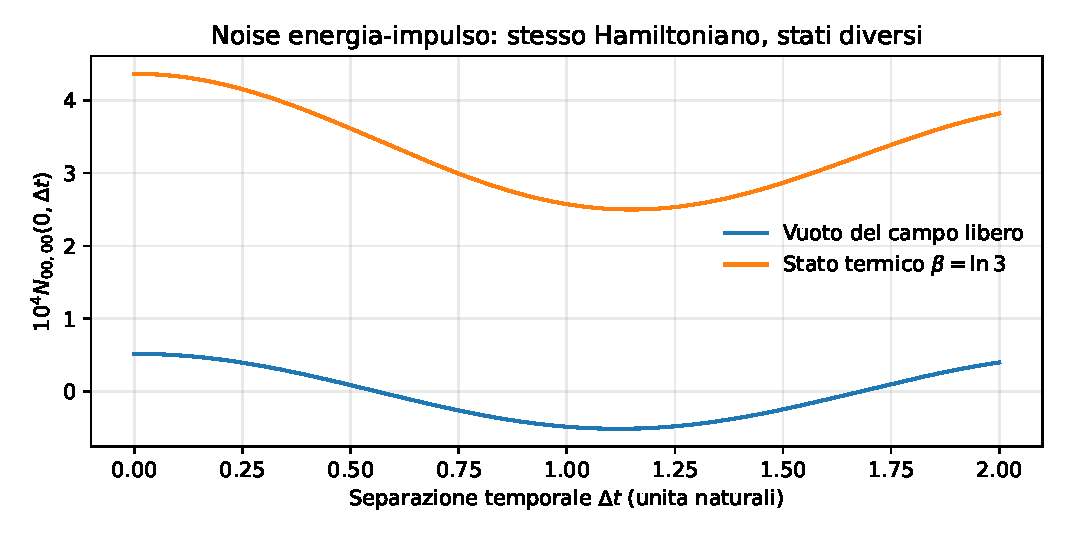
\includegraphics[width=.87\linewidth]{r12av_stress_noise.pdf}
\caption{Noise $\mathcal N_{00,00}$ in funzione della separazione temporale nello stesso punto, sul toro con sette modi. Vuoto e stato termico condividono azione ed equazioni del moto, ma non le fluttuazioni. Grafico diagnostico a cutoff fisso, non previsione cosmologica.}
\label{fig:r12av-stress-noise}
\end{figure}

\subsection{Controllo negativo: il cutoff interrompe la microcausalita esatta}
Una verifica addizionale \emph{post-protocollo, non contata nei test congelati}, impedisce una interpretazione impropria dei risultati. Per $x=(t,\mathbf0)$ e $y=(0,\pi,0,0)$, separati spazialmente quando $0<t<\pi$, il commutatore del campo troncato e
\begin{equation}
 [\hat\phi(x),\hat\phi(y)]
 =-\frac{i}{V}\left[\sin t+\sqrt2\sin(\sqrt2t)\right]\ne0.
 \label{eq:r12av-nonlocal-cutoff}
\end{equation}
A $t=0.1$ il suo modulo e circa $1.2061\times10^{-3}$. Dunque il \emph{cutoff} preserva l'equazione di Klein--Gordon e la Ward algebraica, ma \emph{non} preserva la localita relativistica esatta. Non e consentito dedurre da R12av un noise kernel locale e rinormalizzato senza studiare un limite di rimozione del cutoff e le condizioni distribuzionali appropriate.

\subsection{Verdetto R12av}
Il nuovo controllo colma una lacuna delimitata di R12au: dimostra, in una materia quantistica gaussiana a cutoff finito e background prefissato, che il noise \emph{tensoriale} e calcolabile dalla stessa microdinamica e dallo stato, e che soddisfa positivita e conservazione on-shell. Non ha prodotto la selezione dello stato quantistico della geometria, una somma su causal set dinamici, una Ward gravitazionale quantistica, uno stress rinormalizzato dopo rimozione del cutoff, la risposta metrica autoconsistente o una nuova evoluzione cosmica $H(t)$. \textbf{R12as fisico NON AUTORIZZATO; R13 BLOCCATO.}
\begin{center}\small
\nolinkurl{R12AV_FINITE_BAND_QFT_STRESS_NOISE_WARD_PASS_DYNAMICAL_GRAVITY_NOT_DERIVED_R13_BLOCKED}
\end{center}


\clearpage
\section{Screening R12aw: rimozione del cutoff, microcausalita e fluttuazioni quadratiche}
\label{sec:r12aw-uv}
\textbf{Classificazione: \status{SCREENING UV DEL CAMPO LIBERO: PASS; STRESS COMPLETO E GRAVITA DINAMICA NON DERIVATI}.}

R12av ha verificato positivita e conservazione on-shell del noise del tensore energia--impulso a sette modi, registrando la violazione della microcausalita del campo al cutoff. R12aw non dichiara completata la gravita: studia due questioni \emph{distinte} nel medesimo benchmark libero a metrica fissata, mantenendo tutti i parametri preregistrati. La letteratura tratta gli operatori locali composti come \emph{distribuzioni}, non come variabili con fluttuazione finita in ogni punto; una costruzione covariante completa richiede ulteriori condizioni \cite{HollandsWald2001LocalWick,WuFordSchiappacasse2023,HuVerdaguer2008}.

\subsection{Geometria, vuoto e protocollo congelato}
Su $\mathbb R\times\mathbb T^3$ con $L=2\pi$, $V=L^3$, massa $m=1$ e $c=\hbar=1$, usiamo il campo libero
\begin{equation}
 \hat\phi_K(t,\mathbf x)=\sum_{\|\mathbf k\|_\infty\le K}
 \frac{\hat a_{\mathbf k}e^{-i\omega_{\mathbf k}t+i\mathbf k\cdot\mathbf x}+\hat a_{\mathbf k}^\dagger e^{i\omega_{\mathbf k}t-i\mathbf k\cdot\mathbf x}}{\sqrt{2V\omega_{\mathbf k}}},
 \qquad \omega_{\mathbf k}=\sqrt{1+|\mathbf k|^2}.
 \label{eq:r12aw-field}
\end{equation}
Il cutoff e il cubo simmetrico $\|\mathbf k\|_\infty\le K$. Lo stato di vuoto e \emph{assegnato}; il test non propone una scelta quantistica dello stato cosmologico. Non si usa il valore osservato di $H(t)$, ne un fit dei cutoff ai dati. Questo insieme di modi, che cresce con $K$, non va confuso con il gruppo fisso dei sette modi impiegato in R12av.

\subsection{Microcausalita per due osservabili spazialmente distribuiti}
Definiamo una finestra compatta $b_w(x)=[1+\cos(\pi x/w)]/(2w)$ per $|x|\le w$ e zero altrove sul cerchio, con $w=0.6$. Essa e $C^1$ ed e normalizzata. Consideriamo due osservabili mediati in spazio:
\begin{equation}
 F(\mathbf x)=\frac{b_w(x)}{(2\pi)^2},\quad G(\mathbf x)=\frac{b_w(x-\pi)}{(2\pi)^2},\quad \Delta t=1.1,
 \qquad \pi-2w\simeq1.942>\Delta t.
 \label{eq:r12aw-spacelike}
\end{equation}
Tutti i punti nei due supporti sono separati di tipo spazio. L'integrazione nelle due coordinate trasverse seleziona esattamente i modi $\mathbf k=(n,0,0)$ \emph{dello stesso campo in quattro dimensioni}. Ponendo $a=\pi/w$, la trasformata di Fourier della finestra e
\begin{equation}
 \widehat b_0=1,\qquad
 \widehat b_n=\frac{a^2\sin(nw)}{wn(a^2-n^2)}\quad(n\in\mathbb Z\setminus\{0\}).
 \label{eq:r12aw-fourier}
\end{equation}
Il coefficiente immaginario del commutatore $[\hat\phi_K(F,\Delta t),\hat\phi_K(G,0)]$ e la somma esatta
\begin{equation}
 \mathcal C_K=\frac1V\sum_{n=-K}^{K}(-1)^n|\widehat b_n|^2\frac{\sin(\sqrt{1+n^2}\,\Delta t)}{\sqrt{1+n^2}}.
 \label{eq:r12aw-comm}
\end{equation}
L'equazione di Klein--Gordon ha velocita finita di propagazione: poiche i supporti sono separati spazialmente, nel campo completo $\mathcal C_\infty=0$. Per $n\ge 2a$, $|\widehat b_n|\le4a^2/(3wn^3)$. Si ottiene per ogni intero $K\ge\lceil2a\rceil$ il \emph{bound a priori}
\begin{equation}
 \boxed{|\mathcal C_K|=|\mathcal C_K-\mathcal C_\infty|
 \le\frac{16a^4}{27w^2V}\,K^{-6}.}
 \label{eq:r12aw-micro-bound}
\end{equation}
La crescita del cutoff recupera cosi la microcausalita di questa coppia di \emph{osservabili del campo mediati}, non la microcausalita esatta al cutoff finito. Il residuo puo oscillare e non e necessariamente monotono.

\begin{table}[htbp]\centering\small
\caption{R12aw: commutatore della coppia separata spazialmente. Il bound $K^{-6}$ vale per $K\ge11$; i valori sono coefficienti adimensionali del benchmark.}
\begin{tabular}{rrr}\toprule
$K$ & $|\mathcal C_K|$ & Bound valido a priori \\\midrule
0 & $3.59\times10^{-3}$ & -- \\
8 & $2.23\times10^{-6}$ & -- \\
12 & $3.04\times10^{-7}$ & $1.67\times10^{-6}$ \\
24 & $1.09\times10^{-9}$ & $2.61\times10^{-8}$ \\
64 & $1.91\times10^{-12}$ & $7.26\times10^{-11}$ \\
96 & $1.00\times10^{-13}$ & $6.37\times10^{-12}$ \\
\bottomrule\end{tabular}
\label{tab:r12aw-locality}
\end{table}

\begin{figure}[htbp]\centering
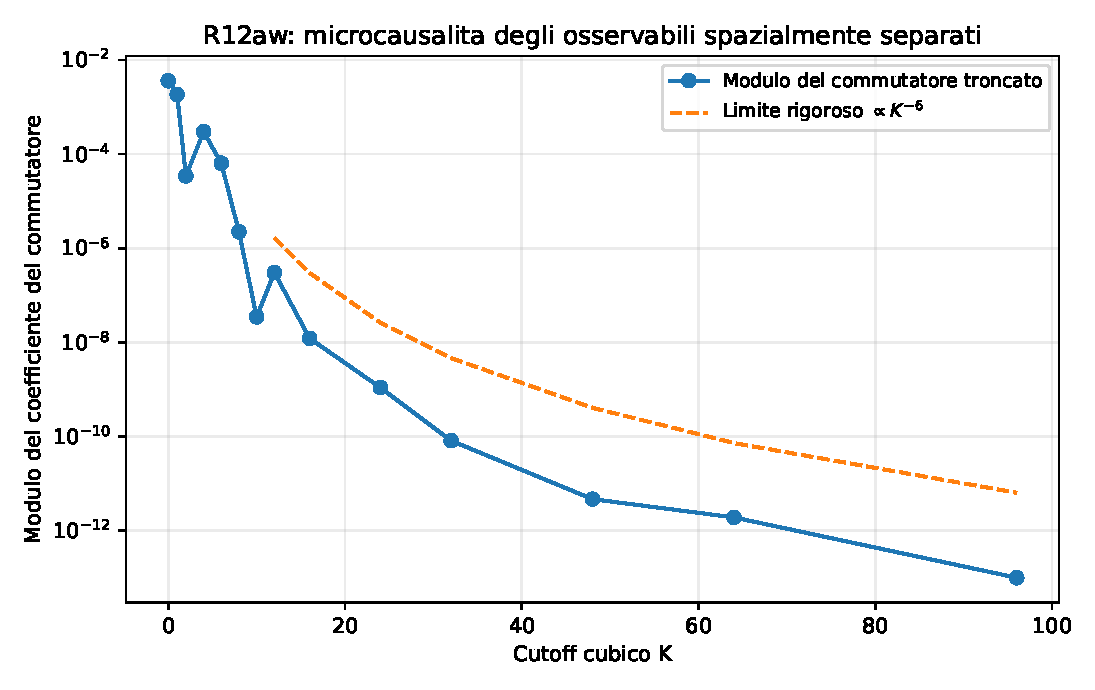
\includegraphics[width=.84\linewidth]{r12aw_field_microcausality.pdf}
\caption{R12aw: residuo del commutatore di due osservabili del campo con supporti separati spazialmente. La linea tratteggiata e il limite superiore matematico, non un fit.}
\label{fig:r12aw-locality}
\end{figure}

\subsection{Fluttuazioni puntuali divergenti del quadrato del campo derivato}
Con $\hat\pi_K=\partial_t\hat\phi_K$, definiamo soltanto il \emph{pezzo quadratico} $\hat W_K(t)=:\!\hat\pi_K(t,\mathbf x_0)^2\!:$, Wick-ordinato nel vuoto. L'identita di Wick fornisce
\begin{equation}
 \boxed{\mathrm{Var}_0[\hat W_K(t)]=\frac{1}{2V^2}
 \left(\sum_{\|\mathbf k\|_\infty\le K}\omega_{\mathbf k}\right)^2
 =\Theta(K^8).}
 \label{eq:r12aw-point-divergence}
\end{equation}
La dimostrazione dell'esponente usa il numero $\Theta(K^3)$ di modi e la scala $\omega_{\mathbf k}=\Theta(K)$ su una frazione fissa del cubo. Sottrarre la media nel vuoto non rende finite le fluttuazioni \emph{nel punto}. La conclusione riguarda questo pezzo $:\!\pi^2\!:$; non e un teorema di divergenza di ogni componente del tensore rinormalizzato.

\subsection{Convergenza certificata dopo una media temporale}
Imponiamo prima dei calcoli una gaussiana temporale di Schwartz $g_\sigma(t)=e^{-t^2/(2\sigma^2)}/(\sqrt{2\pi}\sigma)$, $\sigma=0.5$, e $\hat W_K(g_\sigma)=\int dt\,g_\sigma(t)\hat W_K(t)$. Il teorema di Wick da
\begin{equation}
 \boxed{\mathrm{Var}_0[\hat W_K(g_\sigma)]
 =\frac{1}{2V^2}\sum_{\mathbf k,\mathbf p\in[-K,K]^3}
 \omega_{\mathbf k}\omega_{\mathbf p}
 e^{-\sigma^2(\omega_{\mathbf k}+\omega_{\mathbf p})^2}.}
 \label{eq:r12aw-smeared-variance}
\end{equation}
I termini sono positivi e la serie infinita converge, poiche $(\omega_k+\omega_p)^2\ge\omega_k^2+\omega_p^2$ e $\sum\omega_k e^{-\sigma^2\omega_k^2}<\infty$. Non e una regolazione ad hoc della gravita, ma una regolare media di un osservabile Wick-ordinato nello spazio-tempo fisso. La gaussiana \emph{non} ha supporto temporale compatto e pertanto questo test non autorizza una asserzione di localita esatta dell'osservabile mediato.

Per rendere la convergenza un controllo certificato, siano $A_K=\sum_{\mathrm{in}}\omega_k e^{-\sigma^2\omega_k^2}$ e $T_K=\sum_{\mathrm{out}}\omega_k e^{-\sigma^2\omega_k^2}$. Allora
\begin{equation}
 0\le \mathrm{Var}_\infty-\mathrm{Var}_K
 \le\frac{2A_KT_K+T_K^2}{2V^2}.
 \label{eq:r12aw-tail-noise}
\end{equation}
Un guscio di norma cubica $r\ge1$ contiene $24r^2+2$ modi e fornisce
\begin{equation}
 T_K\le\sum_{r>K}(24r^2+2)\sqrt{1+3r^2}\,e^{-\sigma^2(1+r^2)}.
 \label{eq:r12aw-tail-shell}
\end{equation}
La coda dopo $R=\max(K+1,40)$ e dominata da una serie geometrica con rapporto al piu $q_R=(1+1/R)^3 e^{-\sigma^2(2R+1)}<1$. Questo fornisce un limite \emph{senza fit}. A $K=8$ l'errore assoluto certificato e inferiore a $5.4\times10^{-8}$; a $K=12$ e minore di $4.6\times10^{-17}$ in aritmetica reale, non una pretesa di 17 cifre accurate in floating point.

\begin{table}[htbp]\centering\small
\caption{R12aw: varianza del pezzo $:\!\pi^2\!:$ al punto e dopo media temporale con $\sigma=0.5$. La terza colonna converge mentre la seconda cresce senza limite.}
\begin{tabular}{rrr}\toprule
$K$ & Puntuale & Media temporale \\\midrule
0 & $8.126\times10^{-6}$ & $2.9895\times10^{-6}$ \\
2 & $0.8463$ & $0.00287318$ \\
4 & $84.70$ & $0.00343525$ \\
6 & $1566$ & $0.00343851$ \\
8 & $13260$ & $0.00343851$ \\
12 & $287900$ & $0.00343851$ \\
\bottomrule\end{tabular}
\label{tab:r12aw-noise}
\end{table}

\begin{figure}[htbp]\centering
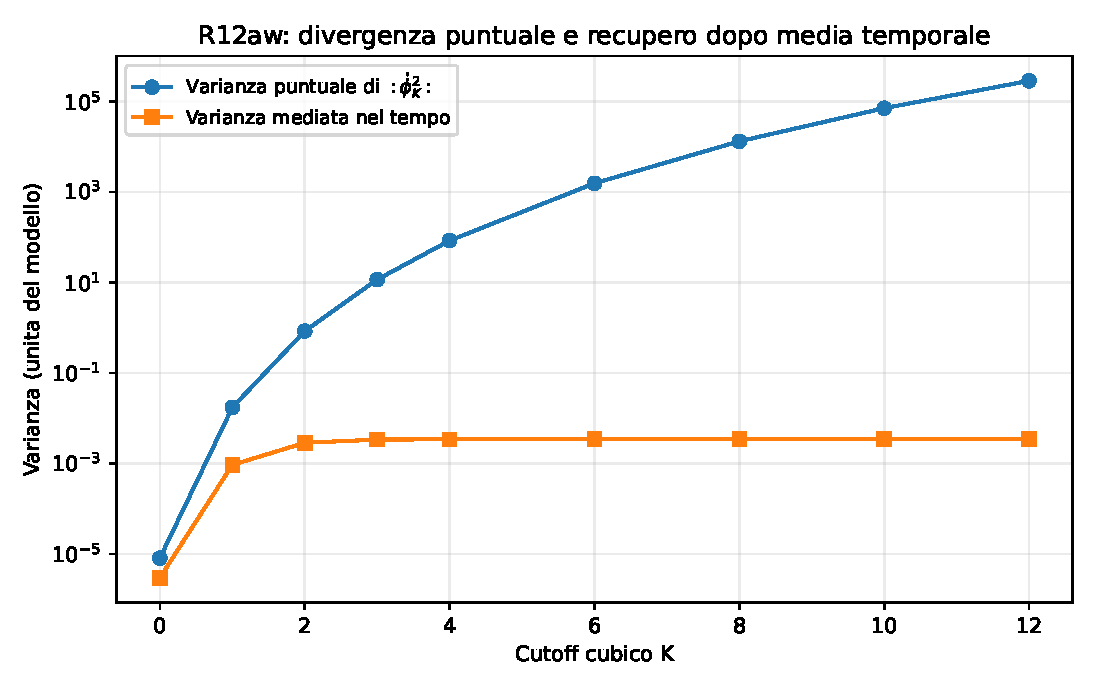
\includegraphics[width=.82\linewidth]{r12aw_uv_smeared_noise.pdf}
\caption{R12aw: varianza puntuale divergente e varianza dello stesso pezzo quadratico dopo smearing temporale. Non rappresenta il noise tensoriale completo e rinormalizzato.}
\label{fig:r12aw-uv}
\end{figure}

\begin{figure}[htbp]\centering
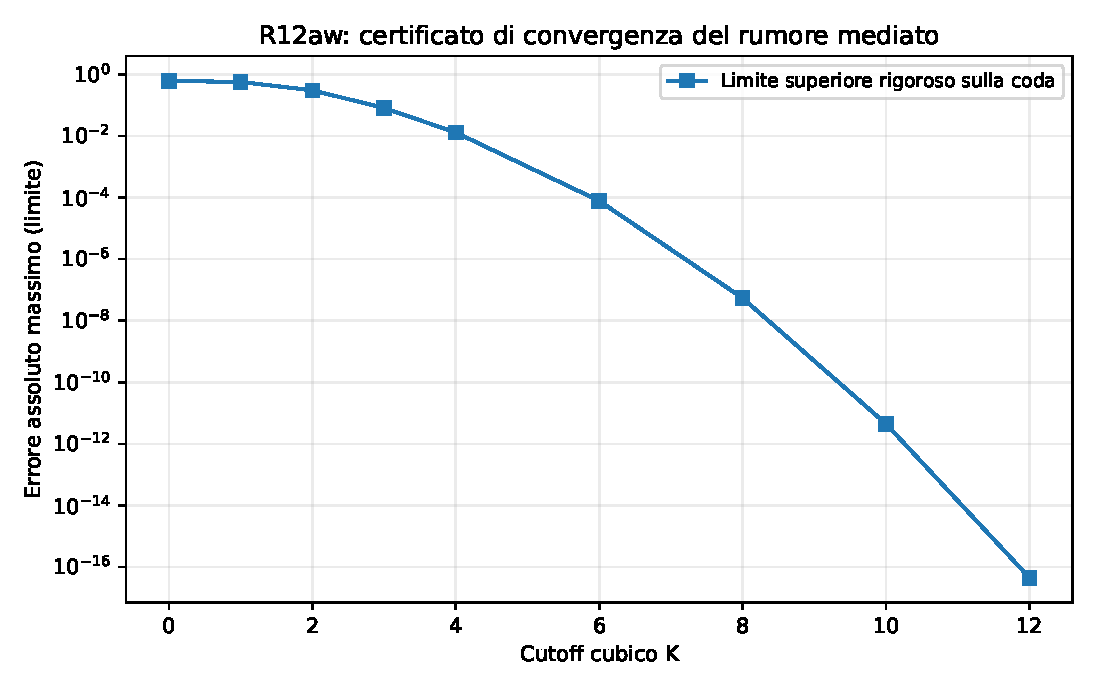
\includegraphics[width=.78\linewidth]{r12aw_tail_certificate.pdf}
\caption{R12aw: limite superiore rigoroso dell'errore assoluto residuo della varianza temporale mediata. L'errore numerico floating point rimane distinto dal bound analitico.}
\label{fig:r12aw-tail}
\end{figure}

\subsection{Validazioni e verdetto fisico}
La preregistrazione e conservata in \texttt{R12AW\_PREREGISTRATION.json}, con SHA-256. Il programma primario ha superato \textbf{15/15} controlli sul limite spaziale, sulla divergenza e sulla coda, mentre il programma indipendente ha superato \textbf{50/50} confronti integrando direttamente la finestra e sommando esplicitamente le coppie di modi per $K\le3$. Nessun parametro e stato selezionato a posteriori. Entrambi i metodi usano soltanto il benchmark di campo libero su \emph{sfondo prefissato}.

\textbf{Conseguenza negativa cruciale:} il recupero del commutatore del campo mediato non e una prova dell'esistenza di un noise tensoriale completo, locale e covariantemente rinormalizzato su geometrie dinamiche; la media temporale gaussiana rende regolare un solo termine Wick-quadratico, non rimuove le ambiguita di rinormalizzazione dell'energia--impulso. Restano anche assenti la misura quantistica 4D delle geometrie causali, la scelta dello stato, la sorgente gravitazionale Ward/Bianchi e una legge cosmologica autonoma. \textbf{R12as fisico NON AUTORIZZATO; R13 BLOCCATO.}
\begin{center}\small
\nolinkurl{R12AW_FIXED_BACKGROUND_UV_FIELD_LOCALITY_AND_SMEARED_WICK_NOISE_PASS_GRAVITY_NOT_DERIVED_R13_BLOCKED}
\end{center}

\section{Screening R12ax: Bell causale operatoriale, identita ternaria e insufficienza per la dinamica 4D}
\label{sec:r12ax}

Il Gate R12aw ha concluso il controllo UV del campo libero su geometria fissata, senza fornire uno stato quantistico delle geometrie dinamiche. Il presente screening si sposta percio sulla \emph{crescita quantistica} dei causal set, ma non assume una nuova legge. Come riferimento esterno si usa il lavoro di Srivastava e Surya pubblicato il 7 ottobre 2026, nel quale differenti ordinamenti della quantum Bell causality (QBC) conducono a vincoli operatoriali distinti \cite{SrivastavaSurya2026}. Le due prescrizioni piu semplici, sotto ipotesi di non singolarita, riconducono a un'algebra commutativa; un terzo ordinamento basato sul passato causale lascia aperta una struttura non commutativa. \textbf{Questi sono risultati della letteratura, non del presente quaderno.}

\subsection{Domanda e preregistrazione}
Il protocollo \texttt{R12AX\_PREREGISTRATION.json} e stato congelato prima dei due programmi di verifica. La domanda e circoscritta: la condizione ternaria necessaria, corrispondente all'Eq.~(114) di \cite{SrivastavaSurya2026},
\begin{equation}
 Q_n Q_k^{-1}Q_m = Q_m Q_k^{-1}Q_n,\qquad k<\min\{n,m\},
 \label{eq:r12ax-ternary}
\end{equation}
impone davvero $[Q_n,Q_m]=0$? Se no, quale livello di selezione fisica resta assente? L'identita e una \emph{condizione necessaria di uno specifico ordinamento}, non l'intera lista delle equazioni di crescita.

\subsection{Un lemma algebrico esatto}
\textbf{Lemma (famiglia a due generatori).} Siano $A$ e $B$ due matrici e sia
\begin{equation}
 Q_j=u_jA+v_jB
\end{equation}
una famiglia di matrici invertibili, con coefficienti scalari. Allora per qualsiasi $n,k,m$,
\begin{equation}
 Q_nQ_k^{-1}Q_m=Q_mQ_k^{-1}Q_n.
 \label{eq:r12ax-lemma}
\end{equation}
\textit{Dimostrazione.} Si scriva $Q_k=uA+vB$. Quando $u\ne0$, moltiplicare $Q_k=uA+vB$ per $Q_k^{-1}B$ a destra e per $BQ_k^{-1}$ a sinistra produce rispettivamente
\begin{align}
 u A Q_k^{-1}B+vB Q_k^{-1}B&=B,\\
 u B Q_k^{-1}A+vB Q_k^{-1}B&=B.
\end{align}
Per sottrazione, $AQ_k^{-1}B=BQ_k^{-1}A$. Se $u=0$, allora $Q_k=vB$ e la stessa uguaglianza vale direttamente. Espandendo il commutatore relativo,
\begin{align}
 &Q_nQ_k^{-1}Q_m-Q_mQ_k^{-1}Q_n\\
 &= (u_nv_m-v_nu_m)
 \bigl(AQ_k^{-1}B-BQ_k^{-1}A\bigr)=0.
\end{align}
La proprieta vale anche quando $A$ e $B$ \emph{non} commutano ordinariamente. $\square$

\subsection{Controesempio positivo e controlli contrari}
Si prenda senza fit la famiglia preregistrata
\begin{equation}
 A=\begin{pmatrix}4&0\\0&1\end{pmatrix},\qquad
 B=\begin{pmatrix}8&2\\2&2\end{pmatrix},\qquad
 Q_1=A,\quad Q_2=B,\quad Q_n=A+(n-2)B\ (n\ge3).
 \label{eq:r12ax-example}
\end{equation}
I minori principali di $A$ e $B$ sono positivi, con $\det A=4$ e $\det B=12$; pertanto ogni $Q_n$ e definita positiva e invertibile. Tuttavia
\begin{equation}
 [A,B]=AB-BA=\begin{pmatrix}0&6\\-6&0\end{pmatrix}\ne0.
 \label{eq:r12ax-noncomm}
\end{equation}
Le identita ternarie valgono comunque per ogni terna, quindi anche per tutte quelle ammesse dalla Eq.~\eqref{eq:r12ax-ternary}. In particolare, si puo avere \emph{commutativita relativa} rispetto al prodotto $XQ_k^{-1}Y$ senza commutativita ordinaria.

La relazione non e priva di forza: con la perturbazione diagnostica fissata prima del test $Q_3\mapsto Q_3+E$, $E=\mathrm{diag}(1,0)$, si ottiene il residuo non nullo
\begin{equation}
 B A^{-1}(Q_3+E)-(Q_3+E)A^{-1}B
 =\begin{pmatrix}0&-\frac12\\\frac12&0\end{pmatrix}.
 \label{eq:r12ax-perturb}
\end{equation}
E per le tre matrici di Pauli differenti si verifica
\begin{equation}
 \sigma_x\sigma_z^{-1}\sigma_y=-iI_2,\qquad
 \sigma_y\sigma_z^{-1}\sigma_x=+iI_2,
\end{equation}
come nel controllo dell'Eq.~(164) di \cite{SrivastavaSurya2026}. Quest'ultimo fallimento non implica che tutte le famiglie matriciali non commutative siano escluse.

\subsection{Replay esatto e ambito limitato}
La stessa lista congelata di confronti e stata eseguita da due programmi indipendenti: \emph{programma SymPy} e \emph{programma a frazioni razionali}. Entrambi passano \textbf{372/372} controlli, di cui \textbf{336} identita ternarie su tutte le terne ordinate di indici distinti da $1$ a $8$. Il confronto fra matrici razionali e esatto; i piccoli residui in aritmetica floating-point nella figura sono \emph{solo} errori numerici della rappresentazione grafica.

\begin{figure}[htbp]
 \centering
 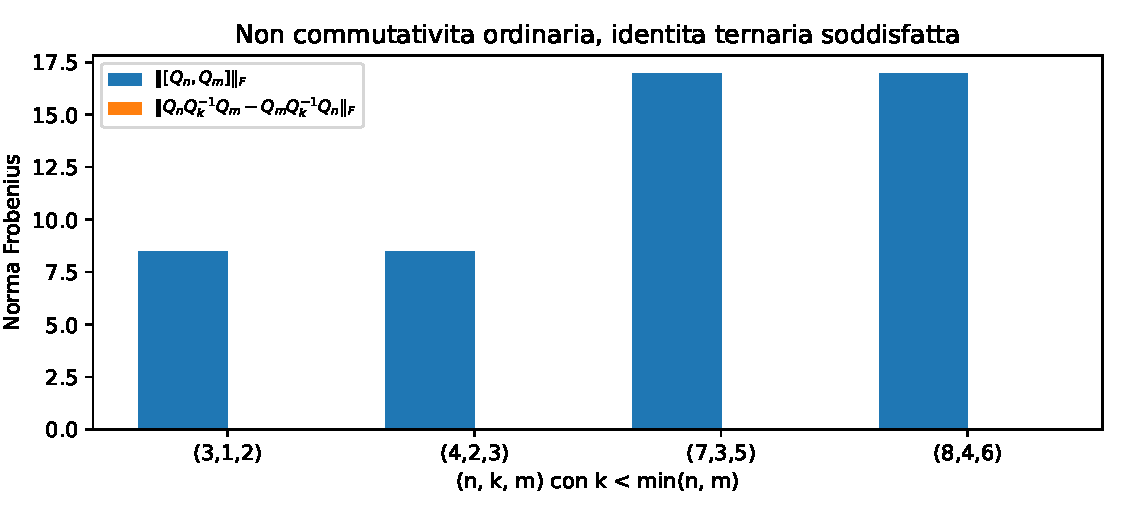
\includegraphics[width=0.88\linewidth]{r12ax_ternary_vs_commutator.pdf}
 \caption{Quattro terne che rispettano $k<\min\{n,m\}$. I normali commutatori fra $Q_n$ e $Q_m$ sono non nulli; i residui della relazione ternaria sono esattamente zero in aritmetica razionale. La figura non verifica l'intera dinamica QSG.}
 \label{fig:r12ax-ternary}
\end{figure}

La famiglia \eqref{eq:r12ax-example} \textbf{non} e una rappresentazione fisica gia ammissibile della crescita: per esempio $I-Q_1=\mathrm{diag}(-3,0)$ e singolare, mentre la costruzione generale citata richiede non singolarita di tutti gli operatori di transizione. Non sono stati verificati la somma di Markov operatoriale, le relazioni Bell ulteriori, la covariance fra tutti i percorsi, una misura con forte positivita estensibile, uno stato quantistico della geometria, un'azione BDG dinamica, Ward/Bianchi, il rumore metrico, la risposta retarded e un limite continuo geometrico 4D. \textbf{Il lemma identifica soltanto la non sufficienza del vincolo ternario isolato.}

\subsection{Decisione e regola di arresto}
\textbf{R12ax: SCREENING ALGEBRICO PASS, DINAMICA QSG/GRAVITAZIONALE NON DERIVATA.} Non si autorizza l'apertura automatica di nuove simulazioni con matrici piu grandi. Un prossimo gate \emph{fisico} dovra prima specificare una microdinamica indipendentemente motivata delle geometrie 4D, con tutte le identita di crescita e la selezione dello stato, oltre a sorgente gravitazionale, conservazione, risposta causale e limite continuo. In assenza di tale ingrediente, \textbf{R12as fisico NON AUTORIZZATO; R13 BLOCCATO.}

\section{Screening R12ay: somma di ampiezze, completezza quantistica e un no-go condizionale}
\label{sec:r12ay}

\subsection{Motivazione, fonti e ipotesi sottoposte al test}
R12ax ha verificato una sola identita ternaria necessaria della quantum Bell causality, senza costruire l'intero albero delle transizioni. Prima di introdurre altre matrici o altri parametri, R12ay confronta due regole di normalizzazione che appartengono a \emph{descrizioni quantistiche diverse}. Nella formulazione operatoriale della crescita sequenziale, la regola forte di somma di Markov ha la forma
\begin{equation}
 \sum_{j=1}^r K_j=I.
 \label{eq:r12ay-markov}
\end{equation}
Per una trasformazione quantistica completamente positiva e conservante la traccia, rappresentata \emph{dagli stessi} operatori di Kraus, la completezza richiede invece
\begin{equation}
 \sum_{j=1}^r K_j^\dagger K_j=I.
 \label{eq:r12ay-kraus}
\end{equation}
La prima struttura e presente nel programma QSG studiato da Srivastava e Surya \cite{SrivastavaSurya2026}; la seconda e standard nella teoria dei canali quantistici \cite{Watrous2018}. \textbf{Imporle simultaneamente agli stessi operatori e un'ipotesi addizionale e restrittiva del presente screening, NON un assioma universale di QSG.} In particolare un'ampiezza di cilindro non e automaticamente un operatore di misura. La domanda e quali ostacoli esatti segua da questa identificazione, e dove tali ostacoli cessino.

Il protocollo \texttt{R12AY\_PREREGISTRATION.json} e stato congelato con SHA-256 prima dei calcoli. Non vengono scelti parametri cosmologici, e il modello resta una algebra matriciale su un nodo astratto di crescita: non e una dinamica delle geometrie 4D.

\subsection{Teorema: con operatori positivi, soltanto proiettori ortogonali}
\textbf{Teorema 1 (doppia normalizzazione positiva).} Siano $K_1,\ldots,K_r$ operatori positivi semidefiniti e autoaggiunti su uno spazio di Hilbert complesso di dimensione finita, con $r\ge2$. Se soddisfano simultaneamente \eqref{eq:r12ay-markov} ed \eqref{eq:r12ay-kraus}, allora sono proiettori ortogonali due a due. Ne segue che non possono essere tutti invertibili se vi sono almeno due rami non nulli.

\textit{Dimostrazione.} Dalla positivita e dalla somma $I$ segue $0\le K_j\le I$. Poiche ciascun autovalore e nell'intervallo $[0,1]$, $K_j-K_j^2\ge0$. Sommando e usando le due normalizzazioni si ottiene
\begin{equation}
 0=\sum_j(K_j-K_j^2).
 \label{eq:r12ay-positive-sum}
\end{equation}
Essendo addendi positivi, ciascuno deve annullarsi: $K_j^2=K_j$. Inoltre per ogni $i$,
\begin{equation}
 0=K_i(I-K_i)K_i=\sum_{j\ne i}K_iK_jK_i.
\end{equation}
Ogni termine e positivo, sicche $K_iK_jK_i=0$ e dunque $K_jK_i=0$ per $i\ne j$. Un proiettore invertibile e necessariamente $I$; due proiettori invertibili non potrebbero quindi sommare a $I$. $\square$

Il risultato \emph{non} esclude ampiezze non positive o non autoaggiunte, ne impone che gli operatori QSG debbano essere Kraus. Isola piuttosto un blocco per l'identificazione piu semplice, quando si desiderino anche transizioni tutte non singolari.

\subsection{Due rami: classificazione completa senza positivita}
\textbf{Teorema 2.} Per due operatori arbitrari quadrati $K_+$ e $K_-$ di dimensione finita, entrambe le regole \eqref{eq:r12ay-markov} e \eqref{eq:r12ay-kraus} valgono se e solo se esiste una matrice unitaria $U$ tale che
\begin{equation}
 K_+=\frac{I+U}{2},\qquad K_-=\frac{I-U}{2}.
 \label{eq:r12ay-two-outcome}
\end{equation}
\textit{Dimostrazione.} La prima regola da $K_-=I-K_+$. Sostituendola nella seconda,
\begin{equation}
 2K_+^\dagger K_+-K_+-K_+^\dagger=0.
\end{equation}
Poni $U=2K_+-I$: l'uguaglianza precedente equivale a $U^\dagger U=I$; per matrici quadrate finite $U$ e unitaria. Inversamente \eqref{eq:r12ay-two-outcome} soddisfa entrambe le somme per ogni $U$ unitaria. Poiche $K_+$ e $K_-$ sono polinomi della \emph{stessa} $U$, \textbf{commutano}, pur non dovendo essere positivi. $\square$

Il controllo esatto fissato nel protocollo usa
\begin{equation}
 U=\begin{pmatrix}3/5&-4/5\\4/5&3/5\end{pmatrix},\qquad
 \det K_+=\frac45,\quad\det K_-=\frac15.
\end{equation}
Entrambi i rami sono invertibili e le due normalizzazioni valgono, ma gli operatori non sono autoaggiunti. Quindi la non invertibilita del Teorema 1 \emph{dipende davvero} dall'ipotesi di positivita.

\subsection{Cinque rami: controesempio razionale non commutativo}
Per evitare di estendere il Teorema 2 indebitamente a un numero qualsiasi di rami, consideriamo le matrici razionali fissate prima dei test,
\begin{equation}
 X=\begin{pmatrix}0&1\\1&0\end{pmatrix},\quad
 Z=\begin{pmatrix}1&0\\0&-1\end{pmatrix},\quad
 \begin{aligned}
 K_1&=\tfrac15I+\tfrac9{25}X,&K_2&=\tfrac15I-\tfrac9{25}X,\\
 K_3&=\tfrac15I+\tfrac{13}{25}Z,&K_4&=\tfrac15I-\tfrac{13}{25}Z,\\
 K_5&=\tfrac15I.&&
 \end{aligned}
 \label{eq:r12ay-five}
\end{equation}
Poiche $X^2=Z^2=I$, i termini lineari si cancellano e si verifica \emph{esattamente}
\begin{equation}
 \sum_{j=1}^5K_j=I,\qquad
 \sum_{j=1}^5K_j^\dagger K_j
 =\left[\frac15+\frac{2(9^2+13^2)}{25^2}\right]I=I.
 \label{eq:r12ay-five-rules}
\end{equation}
Tutte e cinque le matrici sono reali simmetriche e invertibili, ma alcune sono indefinite; si ha inoltre
\begin{equation}
 [K_1,K_3]=\frac1{625}\begin{pmatrix}0&-234\\234&0\end{pmatrix}\ne0.
 \label{eq:r12ay-comm}
\end{equation}
\begin{center}
\begin{tabular}{lccccc}
\toprule
Operatore & $K_1$ & $K_2$ & $K_3$ & $K_4$ & $K_5$\\
\midrule
$\det K_j$ & $-56/625$ & $-56/625$ & $-144/625$ & $-144/625$ & $1/25$\\
\bottomrule
\end{tabular}
\end{center}
Quindi la doppia normalizzazione \emph{da sola} non forza commutativita per un qualunque numero di rami, se si abbandona la positivita. \textbf{Non e tuttavia un modello QSG.} Persino la relazione ternaria necessaria \eqref{eq:r12ax-ternary}, testata sulla tripletta ammessa $k=1<\min\{n=2,m=3\}$, fallisce:
\begin{equation}
 K_2K_1^{-1}K_3-K_3K_1^{-1}K_2
 =\begin{pmatrix}0&-117/70\\117/70&0\end{pmatrix}\ne0.
 \label{eq:r12ay-qbc-fail}
\end{equation}
Questo controllo impedisce di interpretare le cinque matrici come un albero di crescita causal-set gia costruito.

\subsection{Replay, amendment, limiti e verdetto}
Il programma esatto SymPy e quello indipendente a sole frazioni razionali concordano su \textbf{23/23} controlli ciascuno, comprese entrambe le normalizzazioni, i determinanti, i commutatori, un controllo negativo e il test ternario con indice ammesso. Il primo replay aveva usato una tripletta non conforme all'ordinamento di \eqref{eq:r12ax-ternary}: l'errore applicativo e stato registrato in \texttt{R12AY\_TECHNICAL\_AMENDMENT.md} prima del replay valido; nessun parametro e stato modificato. Non si rivendicano fit o estensioni al limite continuo.

\textbf{R12ay: screening matematico PASS. La identificazione positiva Markov--Kraus e esclusa nella classe definita.} Le condizioni di canale quantistico e crescita di ampiezze non devono essere imposte agli stessi operatori senza un principio indipendente. La classificazione a due rami e il controesempio a cinque rami impediscono generalizzazioni oltre le ipotesi. Non sono derivati tutte le transizioni QSG, general covariance, una misura quantistica delle geometrie 4D, Ward/Bianchi, rumore, risposta, limite continuo e $H(t)$. \textbf{R12as fisico NON AUTORIZZATO; R13 BLOCCATO.}

\section{Screening R12az: stato Sorkin--Johnston, positivita finita e restrizione causale}
\label{sec:r12az}

Il Gate R12ay ha mostrato i limiti dell'identificazione non giustificata fra operatori di crescita e operatori di Kraus. Il passo R12az evita una nuova variante di tale costruzione e testa invece un principio indipendente, gia presente nella letteratura: la \emph{prescrizione spettrale di Sorkin--Johnston} (SJ) per uno stato di campo scalare libero su una geometria causale \emph{fissata} \cite{Johnston2009SJ,AfshordiAslanbeigiSorkin2012SJ,Surya2019Review}. Questa scelta fornisce un controllo concreto della selezione dello stato della \emph{materia}, non una selezione dello stato quantistico della \emph{geometria}. Il protocollo e stato congelato prima dei nuovi test con otto fixture finite e nessun fit.

\subsection{Dal propagatore retarded al candidato stato SJ}

Si riutilizza senza modificarlo l'operatore retarded adimensionale $B$ del Gate R12at: $B_{ij}=-\delta_{ij}+b_k$ quando $j\prec i$ e l'intervallo causale aperto contiene $k=0,1,2,3$ elementi, con $(b_0,b_1,b_2,b_3)=(1,-9,16,-8)$; i contributi oltre il terzo strato sono nulli. Si omette il prefattore comune $4/(\sqrt{6}\ell^2)$, senza dedurre da una catena finita alcun limite fisico quadridimensionale. Con prodotto interno uniforme sugli elementi e
\begin{equation}
  G_R=B^{-1},\quad G_A=G_R^{\mathsf T},\quad
  \Delta=G_R-G_A,\quad A=i\Delta=A^\dagger.
  \label{eq:r12az_retarded}
\end{equation}
La regola SJ prende la parte spettrale positiva:
\begin{equation}
  W_{\mathrm{SJ}}=A_+=\tfrac12\bigl(A+\sqrt{A^2}\bigr).
  \label{eq:r12az_positive}
\end{equation}
Poiche $A$ e Hermitiano, $W_{\mathrm{SJ}}$ e Hermitiano e semidefinito positivo, mentre, essendo $A^{\mathsf T}=-A$, vale
\begin{equation}
  W_{\mathrm{SJ}}-W_{\mathrm{SJ}}^{\mathsf T}=i\Delta.
  \label{eq:r12az_ccr}
\end{equation}
Questi fatti sono identita di analisi spettrale: non dimostrano da soli che l'inverso di $B$ sia il corretto propagatore di un campo fisico nel continuo ne che il risultante stato sia Hadamard. Inoltre la prescrizione richiede come \emph{input} sia $G_R$ sia il prodotto interno usato per definire lo spettro: il solo ordine causale non ha selezionato dinamicamente il campo.

\subsection{Un controesempio esatto: regioni annidate}

Il controllo decisivo confronta la catena $C_2$ con il passato causale completo dei primi due elementi della catena $C_3$. Dagli stessi coefficienti storici si ottiene
\begin{equation}
 B_2=\begin{pmatrix}-1&0\\1&-1\end{pmatrix},\qquad
 B_3=\begin{pmatrix}-1&0&0\\1&-1&0\\-9&1&-1\end{pmatrix},
 \label{eq:r12az_Bchains}
\end{equation}
con
\begin{equation}
\Delta_2=\begin{pmatrix}0&1\\-1&0\end{pmatrix},\qquad
\Delta_3=\begin{pmatrix}0&1&-8\\-1&0&1\\8&-1&0\end{pmatrix}.
\label{eq:r12az_Dchains}
\end{equation}
Il blocco principale $2\times2$ di $\Delta_3$ coincide \emph{esattamente} con $\Delta_2$. D'altra parte lo spettro di $A_2=i\Delta_2$ e $\{-1,1\}$, mentre quello di $A_3=i\Delta_3$ e $\{-\sqrt{66},0,\sqrt{66}\}$. In particolare $A_3^3=66A_3$, quindi $\sqrt{A_3^2}=A_3^2/\sqrt{66}$ e
\begin{equation}
W_2=\frac12\begin{pmatrix}1&i\\-i&1\end{pmatrix},\qquad
 W_3\big|_{C_2}=\frac12
 \begin{pmatrix}
 65/\sqrt{66}&i-8/\sqrt{66}\\
 -i-8/\sqrt{66}&2/\sqrt{66}
 \end{pmatrix}.
 \label{eq:r12az_Wchains}
\end{equation}
In particolare,
\begin{equation}
\boxed{\;\bigl(W_3\vert_{C_2}-W_2\bigr)_{00}
=\frac{65}{2\sqrt{66}}-\frac12\simeq3.5004734568\ne0\;}.
\label{eq:r12az_witness}
\end{equation}
Pertanto \textbf{la proiezione spettrale positiva non commuta in generale con la restrizione a una sottoregione causale}, anche quando il commutatore del campo, per le fixture specificate, si restringe correttamente. \emph{Applicare indipendentemente la regola SJ a ogni stadio di una crescita causale non fornisce automaticamente una famiglia proiettivamente compatibile di stati.} Questa e una verifica esatta e finita, non un teorema di impossibilita di ogni dinamica quantistica causal-set.

\subsection{Riproducibilita, dipendenza dalla regione e limiti UV}

La validazione comprende le catene $N=2,\ldots,6$, l'antichain a quattro elementi, un diamante a quattro elementi e due catene disgiunte. Per tutte le otto fixture il controllo spettrale verifica positivita, hermiticita e relazione di commutazione; una seconda implementazione indipendente ricostruisce la relazione causale mediante Floyd--Warshall e la parte spettrale mediante Schur. Il replay esatto con SymPy fornisce il certificato della Eq.~\eqref{eq:r12az_witness}. Due compressioni ($2\to3$ e $3\to4$) conservano $\Delta$ e non $W$, e i controlli di rietichettatura non alterano lo stato astratto. Il primo impiego diagnostico di $\operatorname{sqrtm}(A^2)$ ha segnalato una matrice singolare; e stato conservato come amendment tecnico, sostituendo per il controllo indipendente malcondizionato lo Schur senza cambiare la matematica o i coefficienti.

\begin{figure}[htbp]
\centering
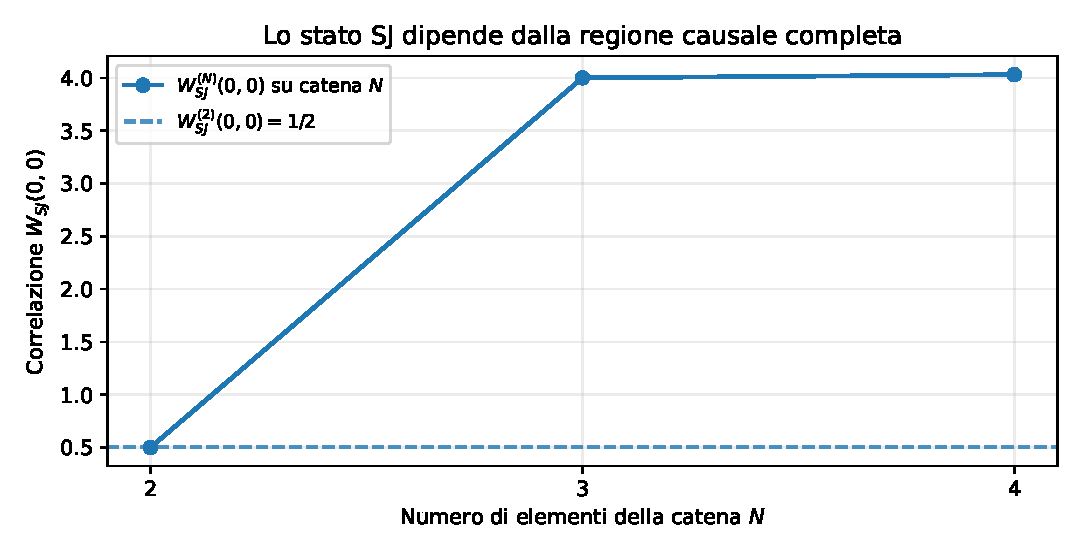
\includegraphics[width=0.82\linewidth]{r12az_nested_state.pdf}
\caption{R12az, sola diagnostica finita: il valore $W_{\rm SJ}^{(N)}(0,0)$ cambia quando la stessa regione iniziale e inclusa in una catena piu lunga. Nessuna legge di scala asintotica o previsione cosmologica e dedotta dal grafico.}
\label{fig:r12az_nested}
\end{figure}

Il risultato costruttivo e solo \emph{uno stato gaussiano di campo libero a causal set finito dato un propagatore e un prodotto interno}. Problemi noti della prescrizione SJ nel continuo includono dipendenza dalla regione e mancata regolarita Hadamard in vari esempi \cite{FewsterVerch2012SJ,FewsterVerch2013Hadamard}. La nostra differenza matriciale tra $W_2$ e $W_3|_{C_2}$ \emph{non} costituisce una prova di inequivalenza di rappresentazioni di Hilbert nello spazio-tempo continuo. Mancano inoltre una misura Lorentziana di geometrie dinamiche, un'origine microfisica dell'azione e dello stato della geometria, una sorgente gravitazionale Ward/Bianchi, un rumore metrico con risposta retarded e il limite continuo controllato. 

\textbf{Verdetto R12az: FINITE SJ MATTER-STATE CONSTRUCTION PASS; NESTED-RESTRICTION COMPATIBILITY FAIL FOR THE EXPLICIT FIXTURES; PHYSICAL QUANTUM-GEOMETRY STATE NOT DERIVED. R12as FISICO NON AUTORIZZATO; R13 BLOCCATO.}

\section{Screening R12ba: triangolazioni causali 4d, volume fissato e selezione cosmologica}
\label{sec:r12ba-screen}

Il precedente R12az selezionava soltanto uno stato di materia su geometria fissata. Per cercare un confronto genuinamente dinamico di \emph{geometrie} 4d, R12ba prende come prior art le \emph{Causal Dynamical Triangulations} (CDT): una somma di triangolazioni causali, governata da un'azione di Regge, calcolata numericamente dopo una continuazione di Wick. Il programma CDT e distinto dalla crescita quantistica di causal set; non si identifica ne la loro misura ne lo spazio delle storie \cite{AmbjornLoll2026CDT,GlaserLoll2017CDT,GizbertStudnicki2024}.

Il controllo e stato preregistrato prima del calcolo, non introduce fit e si limita a una domanda: \emph{il profilo medio tipo de Sitter ottenuto a volume esattamente fissato seleziona da solo il parametro cosmologico?} La risposta analitica e negativa per l'\emph{accoppiamento bare} $\kappa_4$ entro quella specifica distribuzione condizionale; questo non costituisce un no-go su $\Lambda$ fisica renormalizzata o sulla teoria CDT generale.

\subsection{Azione CDT ed ensemble condizionale}

La forma euclidea pertinente contiene \cite{AmbjornLoll2026CDT,GlaserLoll2017CDT}
\begin{equation}\label{eq:r12ba-action}
 S_E(T;\kappa_4,\vartheta)=\kappa_4 N_4(T)+S_0(T;\vartheta),
\end{equation}
dove $N_4$ conta i quattro-simplessi e $\vartheta$ rappresenta gli altri accoppiamenti, inclusi quelli legati a $\kappa_0$ e $\Delta$. Sia $\mathcal T_{\bar N}$ l'insieme delle geometrie con $N_4(T)=\bar N$ \emph{esattamente} fissato. Indicando con $w_0(T;\vartheta)$ un peso non negativo indipendente da $\kappa_4$ (inclusi i fattori di automorfismo), la partizione canonica fattorizza:
\begin{equation}\label{eq:r12ba-Z}
 Z_{\bar N}(\kappa_4,\vartheta)
 =e^{-\kappa_4\bar N}
 \sum_{T\in\mathcal T_{\bar N}}w_0(T;\vartheta).
\end{equation}
Per ogni osservabile $O(T)$ senza dipendenza esplicita da $\kappa_4$, il medesimo fattore si cancella tra numeratore e denominatore:
\begin{equation}\label{eq:r12ba-cancel}
 \boxed{\quad\partial_{\kappa_4}\langle O\rangle_{\bar N}=0,\qquad
 \partial_{\kappa_4}\ln P(T\mid\bar N)=0,\qquad
 I_{\bar N}(\kappa_4)=0.\quad}
\end{equation}
La terza identita indica l'informazione di Fisher del \emph{parametro bare} nel campione \emph{condizionato}. E' un risultato esatto di identificabilita della distribuzione condizionale, non un calcolo di nuovo comportamento dinamico e non una selezione di $\Lambda$.

\subsection{Perche non e un no-go generale}

Quando il volume puo fluttuare, la distribuzione completa e proporzionale a $w_0(T)e^{-\kappa_4N_4(T)}$. Differenziandola si ottengono le identita
\begin{equation}\label{eq:r12ba-grand}
 \boxed{\quad\partial_{\kappa_4}\langle O\rangle
 =-\operatorname{Cov}(O,N_4),\qquad
 I(\kappa_4)=\operatorname{Var}(N_4).\quad}
\end{equation}
Dunque la sensibilita \emph{puo} ricomparire nell'ensemble a volume libero; se viene fissato soltanto $N_{41}$ o si impone una penalita elastica al volume, l'ipotesi esatta dell'Eq.~\eqref{eq:r12ba-cancel} non e automaticamente soddisfatta. CDT contiene inoltre altri accoppiamenti e problemi di scaling e di rinormalizzazione. Il risultato non afferma che la costante cosmologica fisica sia irrilevante o impossibile da determinare in altre condizioni.

\subsection{Profilo euclideo di confronto e limite del suo contenuto}

La quattro-sfera euclidea rotonda di raggio $R$, \emph{non} uno spazio-tempo Lorentziano con una funzione $H(z)$ gia derivata, ha volume spaziale di sezione e quattro-volume
\begin{equation}\label{eq:r12ba-S4}
 V_3(\tau)=2\pi^2R^3\cos^3(\tau/R),\qquad
 V_4=\int_{-\pi R/2}^{\pi R/2}V_3(\tau)\,d\tau
 =\frac{8\pi^2}{3}R^4.
\end{equation}
A scala adimensionale $x=\tau/R$ il profilo normalizzato e
\begin{equation}\label{eq:r12ba-normalized}
 \frac{R V_3(Rx)}{V_4}=\frac34\cos^3 x,
 \qquad -\frac\pi2\le x\le\frac\pi2.
\end{equation}
La forma della curva non determina il raggio assoluto $R$. Solo \emph{assumendo separatamente} la relazione di Einstein per una soluzione classica di vuoto sulla sfera, $\Lambda_{\mathrm{cl}}=3/R^2$, segue l'identita $\Lambda_{\mathrm{cl}}^2V_4=24\pi^2$: una relazione di scala \emph{condizionata}, non un valore previsto a priori. L'emergenza statistica di un profilo $\cos^3$ nella fase CDT e un successo riportato in letteratura \cite{GlaserLoll2017CDT,AmbjornLoll2026CDT}, non una selezione cosmologica autonoma del presente quaderno.

\begin{figure}[htbp]
\centering
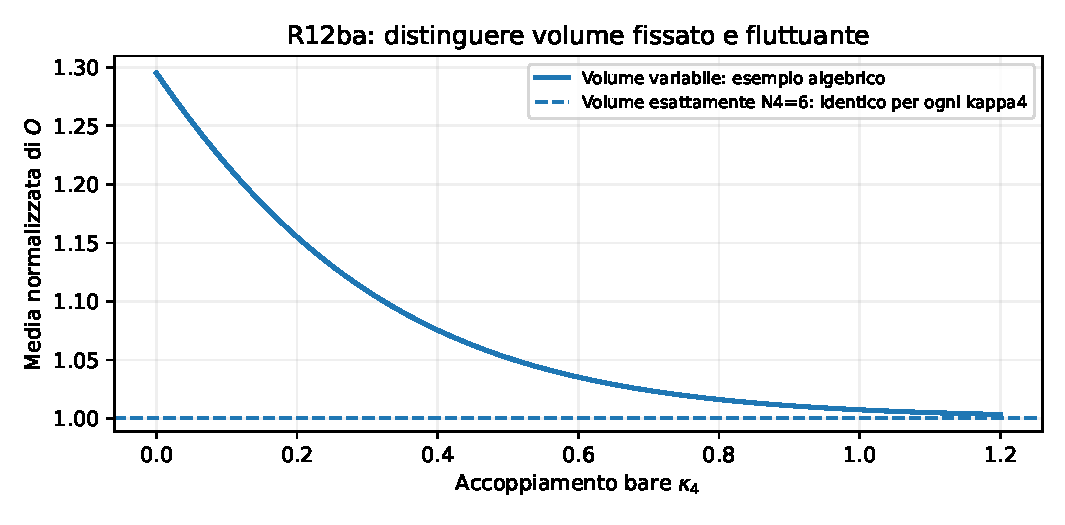
\includegraphics[width=.85\linewidth]{r12ba_fixed_volume_diagnostic.pdf}
\caption{R12ba, illustrazione algebrica \emph{non tratta da dati CDT}: un ensemble toy con $N_4$ fissato ha medie normalizzate indipendenti da $\kappa_4$ (tratteggio); permettendo volumi 6 e 10, la risposta e regolata da $-\operatorname{Cov}(O,N_4)$. Nessun parametro e fittato ai dati cosmologici.}
\label{fig:r12ba-toy}
\end{figure}

\subsection{Validazione e decisione fisica}

Due implementazioni indipendenti hanno controllato le identita, con protocollo fissato prima dei risultati: derivazione simbolica SymPy \textbf{10/10 PASS} e aritmetica razionale \textbf{13/13 PASS}. Il modello finito a quattro storie e solo un sanity check delle somme, non una simulazione di CDT. E' stata verificata anche la contro-identita di volume fluttuante, evitando una conclusione troppo generale. I riferimenti scientifici e i limiti sono registrati nell'audit allegato.

\begin{center}
\begin{tabular}{p{.36\linewidth}p{.53\linewidth}}
\toprule
\textbf{Requisito} & \textbf{Classificazione R12ba}\\
\midrule
Somma su geometrie 4d & Esistente in CDT, \emph{prior art} distinta da causal-set QSG\\
Costante cosmologica bare da profilo a $N_4$ esatto & Non identificabile nell'ensemble condizionale (Eq.~\eqref{eq:r12ba-cancel})\\
Limite continuo / $\Lambda$ fisica & Non stabiliti dall'audit (nessun no-go universale)\\
Misura/stato/azione causal-set 4d unificati & Non derivati nel progetto\\
Sorgente Ward, rumore e risposta metrica & Non derivati nel progetto\\
Legge cosmologica autonoma $H(t)$ & \textbf{R13 BLOCCATO}\\
\bottomrule
\end{tabular}
\end{center}

\textbf{Verdetto R12ba: CDT FIXED-VOLUME IDENTIFIABILITY SCREENING PASS; PHYSICAL TRANSFER NOT DERIVED.} Nessun ingrediente CDT e stato assunto come nuovo principio $c+c$ e non e autorizzato il Gate R12as fisico. La presenza di una geometria media tipo de Sitter \emph{non} sostituisce una legge di espansione cosmologica ottenuta da microdinamica completa. \textbf{R13 BLOCCATO.}


\section{Screening R12bb: bilancio entropia--fase nella sottoclasse bipartita BDG 4d}
\label{sec:r12bb}

Il Gate R12ba ha distinto l'identificabilita di un coupling volumetrico a volume fissato dal problema di una misura sulle geometrie con volume variabile. R12bb torna direttamente alla famiglia causal-set con l'azione 4d \emph{non smeared} di R12aj e isola una sottoclasse per cui \emph{tutta} la somma oscillante e calcolabile esattamente. La domanda non e se il modulo della fase media decada, ma se le cancellazioni siano abbastanza forti da contrastare il numero di geometrie. Il problema generale e noto nella letteratura su ordini non-manifold-like e soppressione Lorentziana \cite{KleitmanRothschild1975,LoomisCarlip2018,Carlip2024}; qui non si rivendica novita fisica ne si adatta un coupling.

\subsection{Sottoclasse etichettata con bipartizione fissata}
Per $N=m+n$ si fissano due insiemi \emph{di etichette} $A$ e $B$ di cardinalita $m=\lfloor N/2\rfloor$ e $n=N-m$. Solo le coppie $a\in A$, $b\in B$ possono essere ordinate, e ciascuna relazione $a\prec b$ puo esserci oppure no. Nessuna relazione puo concatenarsi con un'altra: ogni scelta dei $K=mn$ bit definisce un ordine parziale, per un totale esatto di $2^K$ strutture \emph{con questa bipartizione etichettata fissata}. Non si tratta del conteggio degli ordini \emph{non etichettati}, di tutti i bilayer, o di una misura fisica selezionata.

In questa sottoclasse ogni coppia causalmente correlata e un link: $N_0=k$, $N_1=N_2=N_3=0$, dove $k$ e il numero di relazioni inserite. La Eq.~\eqref{eq:r12aj_action4} si riduce a
\begin{equation}\label{eq:r12bb_action}
\frac{S_4}{\hbar}=a(N-k),\qquad
 a=\frac4{\sqrt6}\left(\frac\ell{\ell_P}\right)^2.
\end{equation}
Con un coupling reale $g$ posto \emph{soltanto} nella funzione caratteristica e $\theta=ga$, il numero di strutture con $k$ link e $\binom{K}{k}$. Quindi
\begin{equation}\label{eq:r12bb_partition}
\boxed{\quad Z_{m,n}(\theta)
 =e^{i\theta N}\sum_{k=0}^{K}\binom Kk e^{-i\theta k}
 =e^{i\theta N}\bigl(1+e^{-i\theta}\bigr)^K.\quad}
\end{equation}
L'identita $1+e^{-i\theta}=2e^{-i\theta/2}\cos(\theta/2)$ separa esattamente la fase media normalizzata $\Phi=Z/2^K$ dalla \emph{somma non normalizzata}:
\begin{equation}\label{eq:r12bb_bases}
\boxed{\quad |\Phi_{m,n}(\theta)|=|\cos(\theta/2)|^K,\qquad
 |Z_{m,n}(\theta)|=\bigl[2|\cos(\theta/2)|\bigr]^K.\quad}
\end{equation}
Per $\theta\not\equiv0\;(\mathrm{mod}\ 2\pi)$ la fase media decade con $K$, ma il modulo di $Z$ \emph{decresce} soltanto se $2|\cos(\theta/2)|<1$. Se questa base e maggiore di uno, il contributo della sottoclasse cresce in modulo anche mentre la fase media si annulla. $\theta=\pi$ produce cancellazione esatta; $\theta=2\pi/3$ e il confine della \emph{sottoclasse fissata}, non un punto critico universale di gravita quantistica.

\subsection{Il coupling storico: due diagnosi opposte}
Si mantengono senza alcuna modifica i valori diagnostici di R12aj, $g=1$ e $\ell/\ell_P=1$, dunque $\theta=4/\sqrt6$. Numericamente
\begin{equation}\label{eq:r12bb_values}
 |\cos(\theta/2)|\simeq0.6847785255,
 \qquad 2|\cos(\theta/2)|\simeq1.3695570510.
\end{equation}
La tabella mostra \emph{valori esatti della formula valutati numericamente}, non simulazioni di una somma su tutte le geometrie.
\begin{center}\small
\begin{tabular}{r r r r}
\toprule
$N$ & $K=mn$ & $\log_{10}|\Phi|$ & $\log_{10}|Z|$\\\midrule
8 & 16 & $-2.631$ & $2.185$\\
16 & 64 & $-10.525$ & $8.741$\\
32 & 256 & $-42.099$ & $34.965$\\
64 & 1024 & $-168.397$ & $139.858$\\
\bottomrule
\end{tabular}
\end{center}
\begin{figure}[htbp]
 \centering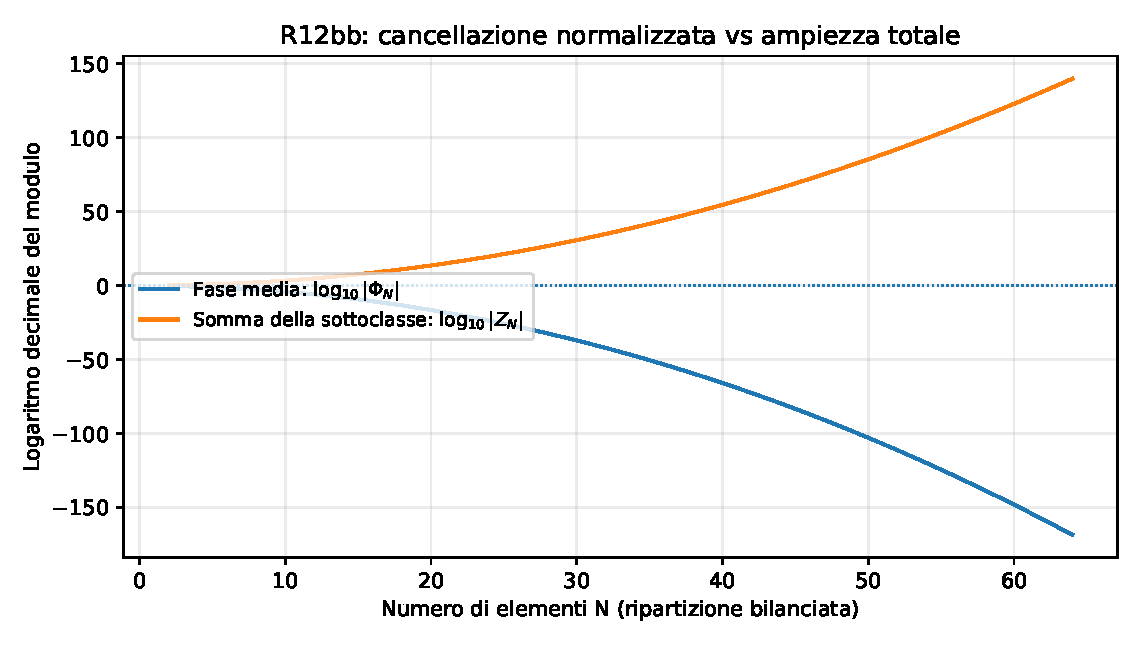
\includegraphics[width=.87\linewidth]{r12bb_exact_phase_entropy.pdf}
 \caption{R12bb, sole curve algebriche dell'ensemble etichettato a due livelli con ripartizione fissata: la fase \emph{normalizzata} diventa minuscola, ma l'ampiezza \emph{non normalizzata} di quel sottoinsieme cresce per il coupling diagnostico storico. Non sono dati cosmologici, un risultato generale sui bilayer non etichettati o una simulazione CDT.}
 \label{fig:r12bb_bases}
\end{figure}

\subsection{Conteggio positivo a volume libero: un no-go ristretto}
L'insieme costruito fornisce un lower bound elementare per il numero di ordini parziali su $N=2m$ etichette. Identificando le strutture fino a isomorfismo si puo perdere al massimo un fattore $(2m)!$, sicche
\begin{equation}\label{eq:r12bb_entropy}
 |\mathcal P_{2m}^{\mathrm{iso}}|\ge\frac{2^{m^2}}{(2m)!}.
\end{equation}
Se si tentasse di normalizzare una \emph{misura positiva uniforme su tutti i poset} di volume variabile mediante il \emph{solo} fattore $e^{-\kappa N}$, per $\kappa$ reale finito, la serie sarebbe divergente. Il rapporto tra termini consecutivi del minorante e
\begin{equation}\label{eq:r12bb_ratio}
\frac{e^{-2\kappa(m+1)}2^{(m+1)^2}/(2m+2)!}
     {e^{-2\kappa m}2^{m^2}/(2m)!}
=\frac{e^{-2\kappa}2^{2m+1}}{(2m+2)(2m+1)}\longrightarrow\infty.
\end{equation}
Questo risultato riguarda \emph{soltanto} la somma positiva ingenua. Non prova divergenza del path sum Lorentziano completo, dove l'azione puo produrre interferenze fra strutture, ne esclude restrizioni di storie, pesi non uniformi o una microdinamica alternativa. La letteratura contiene gia analisi di soppressione dei bilayer piu generali, con ipotesi e regioni di accoppiamento specifiche \cite{LoomisCarlip2018,Carlip2024}.

\subsection{Termine di volume, controlli e verdetto}
A $N$ fissato, aggiungere un termine di fase $\lambda N$ all'azione moltiplica $Z_N$ per $e^{i\lambda N}$, senza alterare $|Z_N|$ o $|\Phi_N|$. Questa identita e il parallelo \emph{Lorentziano e finito} della cancellazione condizionale di R12ba: a volume libero le interferenze \emph{fra diversi} $N$ possono invece dipendere da $\lambda$, senza che il nostro toy selezioni tale parametro.

Il protocollo \texttt{R12BB\_PREREGISTRATION.json} e il suo SHA-256 sono stati fissati prima dei nuovi calcoli. Il programma principale enumera direttamente le $2^{mn}$ configurazioni e i loro intervalli aperti per $N=2,\ldots,8$: \textbf{70.308/70.308 controlli PASS}, con errore massimo assoluto delle somme $8.82\times10^{-13}$. L'implementazione indipendente usa identita binomiali simboliche e somme a 90 cifre: \textbf{28/28 PASS}. Un primo problema di semplificazione simbolica di potenze complesse e registrato come amendment, non eliminato dall'audit.

\textbf{Verdetto R12bb: exact labeled-bipartition entropy--phase benchmark PASS; physical geometric measure/continuum NOT DERIVED.} La sottoclasse non rappresenta il path sum fisico 4d; non sono state derivate misura, selezione di stato geometrico, sorgente Ward/Bianchi, rumore metrico, risposta retarded o una legge $H(z)$. \textbf{R12as fisico NON AUTORIZZATO; R13 BLOCCATO.}


\section{Roadmap cumulativa}

\subsection*{Gate R0 - Definizioni e igiene concettuale}
\begin{enumerate}[label=R0.\arabic*]
\item Non usare ``distanza dal Big Bang'' come distanza da un punto spaziale centrale.
\item Distinguere velocita locale della luce, velocita di recessione, distanza propria e coordinata comovente.
\item Non introdurre un sistema di riferimento del fotone.
\item Sostituire ``prima luce'' con un oggetto fisicamente definito: fronte causale primordiale, orizzonte delle particelle o fotoni free-streaming post-disaccoppiamento, a seconda del test.
\end{enumerate}

\subsection*{Gate R1 - Due fotoni co-propaganti}
Derivare e conservare come baseline Eqs.~\eqref{eq:comoving_constant} e \eqref{eq:coprop_separation}. Ripetere i controlli con emissioni da posizioni diverse e con curvatura spaziale non nulla.

\subsection*{Gate R2 - Due fronti opposti}
Studiare Eq.~\eqref{eq:master_two_rays} e separare esplicitamente il contributo causale $2c$ dal termine geometrico $HD$.

\subsection*{Gate R3 - Dizionario delle distanze}
Seguire gli stessi segnali usando distanza propria, distanza comovente, tempo conforme, distanza di luminosita e distanza angolare. Evitare confronti tra quantita non equivalenti.

\subsection*{Gate R4 - Orizzonti}
Calcolare $R_p$, $R_e$, $R_H$ e $R_A$ nella stessa cosmologia e verificare quando coincidono o divergono.

\subsection*{Gate R5 - Era radiativa}
Formalizzare il risultato speciale $R_p=R_H=2ct$ e determinare se possiede una interpretazione causale piu profonda oppure se e soltanto la conseguenza di $a\propto t^{1/2}$.

\subsection*{Gate R6 - Dinamica di $\alpha$}
Usare
\begin{equation}
 \alpha=HR_p/c,\qquad q=(1-\alpha')/\alpha
\end{equation}
come parametrizzazione diagnostica. Vietato scegliere $\alpha(a)$ per fit a posteriori senza principio indipendente.

\subsection*{Gate R7 - Diagnostica $\beta$}
Usare $\beta=H\Delta D/c$ per quantificare l'esperimento dei due fotoni, verificando la transizione tra decelerazione e accelerazione tramite Eq.~\eqref{eq:beta_q}.

\subsection*{Gate R8 - Chiusura termodinamica/informazionale -- COMPLETATO}
Esito: la termodinamica standard dell'orizzonte apparente riproduce le equazioni di Friedmann, ma non determina autonomamente $p(\rho)$ e quindi non chiude $\alpha(t)$. Il particle horizon non puo essere promosso a schermo termodinamico equivalente senza ipotesi aggiuntive.

\subsection*{Gate R9 - Passato/futuro causale -- COMPLETATO}
Introdotta $\varepsilon=R_e/R_A$ e derivata la coppia $\alpha'=1-q\alpha$, $\varepsilon'=-1-q\varepsilon$. Derivata inoltre l'interpolazione esatta $\alpha:1\to2$ nel sistema radiazione--materia. Una fase accelerata richiede nuova dinamica o contenuto energetico, non segue dalla causalita sola.

\subsection*{Gate R9b - Conservazione e covarianza}
Ogni legge candidata deve rispettare la conservazione covariante dell'energia-impulso o esplicitare in modo consistente perche e modificata. Nessuna somma non relativistica di velocita e ammessa.

\subsection*{Gate R10 - Chiusura entropica $S(A)$ -- COMPLETATO}
Derivata la mappa generale Eqs.~\eqref{eq:generic_entropy_raychaudhuri}--\eqref{eq:entropy_friedmann_integral}. Potenza costante e correzione logaritmica falliscono come chiusure minime universali; una forma tipo Renyi sopravvive come toy model gia noto, ma non e derivata dall'intuizione causale.

\subsection*{Gate R11 - Flusso energia/informazione sull'orizzonte -- COMPLETATO}
Testati Landauer, saturazione del bound di Bekenstein, holographic equipartition e un bilanciamento diretto $S_p/S_A$. I primi tre ricostruiscono o riformulano equazioni gia presenti; il quarto equivale a imporre $\alpha'=0$. Nessuna chiusura autonoma di $H$ o $\alpha$ e stata derivata.

\subsection*{Gate R12 - Dinamica causale del contenuto energetico -- COMPLETATO}
Testate densita $L^{-2}$ basate su $R_p$, $R_A$, $R_e$, la scala conforme $\eta$ e un toy simmetrico passato--futuro. Derivato un no-go ristretto per sorgenti totali a coefficienti costanti costruite da $R_p^{-2}$ e $R_A^{-2}$. Il particle horizon traccia il background; l'apparent horizon e tautologico; l'event horizon accelera ma dipende dal futuro. Il conformal-age cutoff sopravvive come benchmark gia noto, non come derivazione nuova.

\subsection*{Gate R12b - Origine della scala conforme -- COMPLETATO}
La sola struttura nulla non seleziona $\eta^{-2}$ in modo indipendente dalla normalizzazione del fattore di scala. Derivato inoltre un tracking theorem ristretto per densita scale-free $\rho_cF(\alpha,\alpha',q,\ldots)$: in una esatta era di potenza la frazione energetica resta costante.

\subsection*{Gate R12c - Una sola nuova scala -- COMPLETATO}
La famiglia $\rho_X\propto L_*^{n-2}R_p^{-n}$ rompe il tracking per $n<2$. Il caso $n=0$ e una costante cosmologica; il caso genuinamente causale minimo $n=1$ produce una sequenza radiazione--materia--accelerazione a livello di background ma coincide con Tsallis HDE a $\delta=3/2$. Ne $n$ ne $L_*$ sono derivati dalla causalita.

\subsection*{Gate R12d - Interazione o memoria covariante -- COMPLETATO}
Una interazione puo rendere piu negativa la pressione efficace, ma per $R_p^{-2}$ l'accelerazione implica $\Omega_p'<0$ e quindi non corrisponde a un takeover della componente causale. Il flusso di sweep del particle horizon e bookkeeping di un volume mobile, non un nuovo $Q$. Le memorie retarded dimensionali minime tracciano il background; memorie adimensionali secolari come $-\Box^{-1}R$ possono rompere il tracking ma richiedono una funzione di distorsione o una nuova scala per diventare dinamica.

\subsection*{Gate R12e - Congruenza nulla e principio di selezione -- COMPLETATO}
La Raychaudhuri nulla del fascio FLRW shear-free recupera la combinazione $\dot H-k/a^2=-4\pi G(\rho+p)$, quindi la parte derivativa di Friedmann. E cieca a $p=-\rho$ e a $\Lambda g_{\mu\nu}$; con la conservazione si integra soltanto fino a una costante cosmologica non determinata. Sul piano cinematico, nel caso piatto un raggio uscente istantaneamente posto su $R_A=c/H$ soddisfa $\dot R_+=2c$ e quello entrante $\dot R_-=0$, mentre $\dot R_A=c(1+q)$. La boundary condition locale del fronte primordiale non seleziona la costante di integrazione.

\subsection*{Gate R12f - Origine della costante di integrazione -- COMPLETATO}
Entanglement equilibrium non seleziona il valore assoluto di $\Lambda$; la gravita unimodulare lo promuove a costante/grado globale che richiede dati di stato; il sequestering usa vincoli sul quattro-volume ma introduce struttura globale e, nella formulazione originale, dipendenza dalla storia futura. Il ramo causal-set Everpresent $\Lambda$ usa invece il volume del passato causale e produce $\Lambda_{\rm rms}\sim V_4^{-1/2}$, ma resta stocastico e richiede microfisica/ampiezza non derivata. Per $a\propto t^p$ e stato derivato $V_4\propto t^4$, quindi la frazione rms traccia il background.

\subsection*{Gate R12g - Microstruttura causale e legge stocastica covariante -- COMPLETATO}
Nel toy cumulativo a contributi condivisi, la correlazione e fissata dal volume di overlap dei passati: $\mathcal C=V(P_x\cap P_y)/\sqrt{V_xV_y}$. Per coni annidati in ere di potenza, $\mathcal C=(t_1/t_2)^2$; per eventi simultanei in Minkowski e stato derivato un kernel compatto esatto e la generalizzazione FLRW e data da un integrale geometrico senza kernel fenomenologico. L'ampiezza resta legata a una scala di discrezione non derivata. Soprattutto, una $\Lambda(x)g_{\mu\nu}$ locale viola la conservazione separata della materia salvo $\partial\Lambda=0$: manca un completamento covariante conservato unico.

\subsection*{Gate R12h - Completamento stocastico conservato -- COMPLETATO}
La conservazione puo essere ripristinata, ma non in modo unico. Una proiezione trasversa retarded e covariante a livello efficace ma richiede un operatore nonlocale, Green function e boundary data; il completamento a fluido efficace conserva separatamente la materia modificando la pressione; il vero vuoto stocastico mantiene $p=-\rho$ ma Bianchi forza un transfer totale verso gli altri settori. L'unimodularita locale riproduce lo stesso vincolo. Inoltre il kernel di overlap e non differenziabile in media quadratica nel limite continuo, quindi un transfer locale richiede regolarizzazione o stochastic calculus.

\subsection*{Gate R12i - Rumore tensoriale causale conservato -- COMPLETATO}
Il kernel scalare di overlap non seleziona la polarizzazione tensoriale: nel benchmark piatto la conservazione lascia almeno i settori spin--2 e spin--0 trasversi con spettri indipendenti. Un causal set marcato fattorizza la geometria di overlap da una covarianza tensoriale microscopica addizionale. Stochastic gravity conferma che il noise bitensor viene fissato dalla microfisica del vero tensore energia--impulso, non dalla sola causalita.

\subsection*{Gate R12j - Azione stocastica causale e Ward identity -- COMPLETATO}
Una vera azione diffeo-invariante rende la conservazione una Ward identity solo dopo aver messo on-shell tutti i gradi di liberta che trasformano; uno scalare casuale esterno $\lambda(x)$ non diventa quindi automaticamente una sorgente conservata. A livello quadratico Ward lascia form factor trasversi spin--2 e spin--0 indipendenti. Le azioni BDG forniscono il benchmark discreto corretto per il primo cumulante, il cui limite tende a Einstein--Hilbert piu boundary terms, ma media e secondo cumulante sono dati distinti e le costruzioni smeared introducono una nonlocality scale per controllare le fluttuazioni.

\subsection*{Gate R12k - Secondo cumulante dell'azione causale e scala mesoscopica -- COMPLETATO}
Derivato il criterio di matching: se $\mathrm{Var}(S_{\rm BDG})\propto N^\gamma$, allora una sorgente Everpresent richiede $\gamma=1$. Il formalismo moderno delle correlazioni causal-set rende la varianza calcolabile ma non ne ha ancora determinato l'asintotica in Minkowski/FLRW. Le costruzioni smeared introducono $\ell_k>\ell$ e sopprimono le fluttuazioni a $\ell_k$ fisica fissata nel limite continuo; mantenere un rumore fisico finito richiede running/critical scaling. Il coarse-graining/RG causal-set esiste come programma, ma non seleziona ancora ne la mesoscale ne il fixed point $\gamma=1$.

\subsection*{Gate R12l - Scaling quantistico del path sum e secondo cumulante -- COMPLETATO}
Separata la varianza di sprinkling dalla varianza della misura dinamica. Nel benchmark dei 2d-orders, con $\bar\beta=\beta N$ fissato, i risultati di finite-size scaling implicano $\mathrm{Var}(S)\sim N^2$ nella fase continuum-like, $N^3$ nella fase cristallina e $N^4$ al picco di coesistenza di primo ordine: il noto phase structure non seleziona quindi $\gamma=1$. Questo non e un no-go 4d Lorentziano: il path sum reale puo sopprimere classi non-manifold-like, ma il secondo cumulante quantistico nel settore manifold-like non e ancora noto.

\subsection*{Gate R12m - Misura quantistica conservata e protocollo numerico del cumulante -- COMPLETATO}
Protocollo preregistrato e congelato prima dei risultati. Il controllo sintetico recupera $\gamma=0.9930$; il benchmark fixed-$N$ di sprinkling fornisce $\gamma_{\rm spr}=1.8574$ e il Gibbs continuum-like a $\bar\beta=20$ fornisce $\gamma_{\rm G}=1.6368$. Entrambi respingono il target estensivo secondo i criteri congelati, mentre il braccio MCMC supera il quality gate ESS. Il risultato Gibbs non viene identificato con il cumulante Lorentziano $\gamma_Q$.

\subsection*{Gate R12n - Characteristic function / density of states Lorentziana -- COMPLETATO}
Exact enumeration del benchmark representation-weighted per $N=4$--$10$, density of states senza binning e somme a 80 cifre sulla characteristic function. Il protocollo congelato produce $\gamma_Q^{\rm rep}=1.1807$, $R^2=0.9932$, con entrambi i fit endpoint compatibili con il target e sign problem mild ($\min|\phi_N(1)|=0.7775$). Classificazione: \texttt{CONSISTENT\_WITH\_EXTENSIVE\_REP}. Il risultato non e ancora asintotico, unlabeled o 4d.

\subsection*{Gate R12o - Estensione controllata della DOS Lorentziana e onset del sign problem -- COMPLETATO}
Estimatore Monte Carlo diretto validato contro la DOS esatta R12n con errori sub-percentuali. Un milione di permutazioni indipendenti per taglia su $N=12$--$64$ mostra il collasso dell'average phase a $g=1$: soltanto $N=12$--$24$ supera i quality gate preregistrati. Le pendenze locali affidabili sono superestensive ($1.61$--$1.93$), ma con cinque taglie valide il protocollo vieta un fit primario; da $N=32$ il cumulante e gia troppo incerto e da $N=48$ la fase non e risolta. Classificazione: \texttt{FINITE\_SIZE\_OR\_SIGN\_INCONCLUSIVE}.

\subsection*{Gate R12p - Ricostruzione cumulante della DOS / mitigazione del sign problem -- COMPLETATO}
Protocollo preregistrato con cumulanti ordinari fino a $K=12$ e ordine primario $K=10$. La ricostruzione di $\log\phi$ passa exact $N=8$--$10$ e direct-MC fino a $N=20$, ma a $N=24$ fallisce il cumulante connesso: errore primario circa $65\%$ e forte instabilita tra $K=8,10,12$. Classificazione: \texttt{CE\_METHOD\_VALIDATION\_FAIL}. Come imposto prima dei risultati, nessuna estensione $N\ge32$ e stata campionata.

\subsection*{Gate R12q - Density of states globale Wang--Landau / multicanonica -- COMPLETATO}
Il core DOS e molto accurato quando la replica raggiunge la stopping rule: exact $N=8$--$10$ e direct-MC fino a $N=24$ restano entro le soglie numeriche. Tuttavia la robustezza preregistrata richiede almeno tre repliche convergenti su quattro e fallisce a $N=9$ ($2/4$) e $N=12$ ($1/4$). Classificazione: \texttt{DOS\_METHOD\_VALIDATION\_FAIL}. Nessuna estensione $N>24$ viene autorizzata e la schedule non viene corretta post hoc.

\subsection*{Gate R12r - LLR histogram-free / log-DOS slopes -- COMPLETATO}
Protocollo congelato dopo development pilot $N=6,7$ esclusi. Finestre $\Delta S=0.6$ con overlap minimo 50\%, root locale e Robbins--Monro. Exact $N=8$ supera sia accuratezza sia robustezza, mentre $N=9$ e $N=10$ hanno soltanto una replica valida su tre contro il minimo preregistrato di due. Classificazione: \texttt{LLR\_METHOD\_VALIDATION\_FAIL}. Direct validation ed estensione non autorizzate.

\subsection*{Gate R12s - Soft-window umbrella / replica exchange DOS -- COMPLETATO}
Umbrella armoniche, replica exchange e MBAR eliminano il failure di mobilita delle hard windows e superano l'exact gate con tre repliche valide su tre. La direct validation passa fino a $N=20$ ma fallisce fail-closed a $N=24$ appena oltre entrambe le soglie congelate. Classificazione: \texttt{R12S\_METHOD\_VALIDATION\_FAIL}; nessuna estensione $N>24$.

\subsection*{Gate R12t - Phase-targeted bridge / stratified complex reweighting -- COMPLETATO}
Stratificazione indipendente con tre stream uniformi separati: quantili per definire gli strati, un secondo stream per le masse $p_j$ e un terzo per $15\,000$ momenti complessi condizionati per strato. Exact $N=8$--$10$ e direct $N=12$--$24$ passano integralmente; l'estensione e quindi autorizzata. $N=32$ mantiene due repliche coerenti, mentre $N=40,48,64$ non raggiungono il minimo preregistrato. Classificazione: \texttt{R12T\_FINITE\_SIZE\_OR\_PRECISION\_INCONCLUSIVE}; nessun fit globale di $\gamma$.

\subsection*{Gate R12u - Lehmer-ANOVA control variates / Rao--Blackwell locale -- COMPLETATO}
Il codice di Lehmer rende disponibili controlli a media zero esatta. Main effects e interazioni tra digit adiacenti passano exact/direct fino a $N=24$, ma la riduzione di varianza decade con la taglia e scompare attorno a $N=32$. Nell'estensione rimane una sola replica valida a $N=32$ e nessuna a $N=40,48,64$; classificazione \texttt{R12U\_FINITE\_SIZE\_OR\_PRECISION\_INCONCLUSIVE} e nessun fit globale.

\subsection*{Gate R12v - Sign-problem cost law / efficiency frontier -- COMPLETATO}
Derivata la MSE esatta dell'average phase diretto e la influence-function asymptotica del plug-in $\kappa_2$. I dati R12o saturano la previsione statistica fino alla frontiera risolta: a $N=32$ servono circa $1.66\times10^6$ campioni iid per un $15\%$ su $\kappa_2$, mentre a $N=40$ la richiesta sale a circa $1.15\times10^8$. Sul range $N=12$--$40$, $-2\log|\phi|/\mathrm{Var}_0(S)=0.89$--$0.98$, quindi la perdita di fase e in larga misura governata dalla varianza ordinaria dell'azione. Classificazione: \texttt{DIRECT\_COST\_LAW\_DERIVED\_NO\_ASYMPTOTIC\_ESCAPE\_DERIVED}.

\subsection*{Gate R12w - Large-deviation / finestra Fourier del surrogate -- COMPLETATO, INTERPRETAZIONE CORRETTA}
Holdout fresco indipendente: $\mathrm{Var}(S)=0.00640\,N^{2.004}$ sul range $N=24$--$64$ (\emph{fit strettamente limitato a quella finestra; R12aa misura un calo di $\mathrm{Var}(S)/N^2$ fino a $N=1024$}), quasi-collasso di $X_N=(S-4)/N$ e identita $\phi_N(g)=e^{4ig}\widehat f_N(gN)$. Il sestico passa exact/direct come surrogate troncato sulla finestra implementata; R12x mostra che non e una densita globale identificata. Lo status storico R12w viene mantenuto per audit ma la lettura scientifica globale e ritirata.

\subsection*{Gate R12x - Complex-saddle topology / identifiability audit -- COMPLETATO}
Audit dei punti critici: $9/33$ continuazioni sestiche hanno un massimo globale remoto fuori da $|z|=10$. Un programma dei momenti troncato mostra inoltre che gli stessi $m_0,\ldots,m_6$, persino sul supporto osservato, consentono quasi tutto l'intervallo $[-1,1]$ per le componenti della fase a $N=48$--$64$. Classificazione: \nolinkurl{R12X_GLOBAL_ANALYTIC_CONTINUATION_NOT_IDENTIFIED_STOKES_ANALYSIS_NOT_AUTHORIZED}.

\subsection*{Gate R12y - Permuton-only action / controesempi deterministici -- COMPLETATO}
Derivato un confronto al permuton diagonale e uno piu forte al permuton uniforme, con limiti normalizzati dell'azione distinti. Analisi esatta dei conteggi, convergenza dominata e test storico indipendente PASS. Classificazione: \nolinkurl{R12Y_PERMUTON_ONLY_NORMALIZED_ACTION_NO_GO_EVEN_AT_LEBESGUE_PERMUTON}. Non e una conclusione sulla probabilita di tali sequenze sotto misura uniforme.

\subsection*{Gate R12z - Profilo degli intervalli, deriva logaritmica e cancellazioni -- COMPLETATO}
Dimostrata esattamente la formula per $\mathbb E[N_k]/N$ e l'identita $\mathbb E[S_N]=4[1-(1-\epsilon)^N]$. Il profilo grezzo ha medie che crescono come $\ln N$ a cardinalita fissata; la cancellazione firmata dell'azione e esatta. Validazione esaustiva $N=2$--$7$ e campionamenti nuovi $N=16$--$256$ PASS, senza fit. Le code del profilo \emph{centrato} sono verificate soltanto numericamente a taglie finite. Classificazione: \nolinkurl{R12Z_EXACT_MEAN_CANCELLATION_PASS_RAW_PROFILE_DIVERGENT_MEANS_JOINT_LDP_OPEN}.

\subsection*{Gate R12aa - Curvatura discreta e cutoff logaritmico -- COMPLETATO}
Con la seconda differenza dei conteggi, la media esatta del profilo compensato e finita a $k$ fissato; per $K_N=\lceil1.5\ln N/(-\ln(1-\epsilon))\rceil$ l'errore su $S_N/N$ tende a zero uniformemente su tutte le permutazioni. Esistono controesempi per ogni cutoff fisso $K$. Enumerazione esaustiva fino a $N=8$ e holdout $N=64$--$1024$ PASS. Tightness probabilistica, legge limite e LDP congiunta restano aperte. Classificazione: \nolinkurl{R12AA_EXACT_CURVATURE_AND_LOG_CUTOFF_PASS_FIXED_K_UNIFORM_NO_GO_TYPICAL_LIMIT_OPEN}.

\subsection*{Gate R12ab - Covarianze finite-N / criterio di concentrazione -- COMPLETATO}
Derivata la probabilita congiunta esatta di due conteggi di intervalli, distinguendo intervalli disgiunti e sovrapposti; ottenuta la matrice $\Sigma_N(k,l)$ in somma finita esatta. Enumerazione completa $N=3$--$8$ e somma indipendente delle coppie $N\le6$ PASS; holdout congelati $N=64$--$1024$ PASS. Una concentrazione in $L^2$ di $Y_N$ equivale a $Q_{N,K_N}\to0$; nessuna stima asintotica di tale forma quadratica e ancora dimostrata. Classificazione: \nolinkurl{R12AB_EXACT_COVARIANCE_REPRESENTATION_PASS_CONCENTRATION_OPEN}.

\subsection*{Gate R12ac - Bound asintotico della forma quadratica -- COMPLETATO}
La rappresentazione iid dei 2d-orders consente il controllo delle variazioni di un singolo punto tramite rettangoli contenenti o incidenti al punto. Le stime esponenziali per coppie di rettangoli (inclusi estremi condivisi) e Efron--Stein dimostrano $\mathrm{Var}_0(S_N)\le C_\epsilon N(1+\ln N)^2$, quindi $Q_{N,K_N}\to0$. I test preregistrati sono PASS; le inferenze alla misura Lorentziana e al path sum 4d restano vietate.

\subsection*{Gate R12ad - Fluttuazioni finite-$N$ e finestra Fourier -- COMPLETATO CON LIMITI}
\texttt{R12AD\_PREREGISTRATION.json} congelato; 16 taglie con tre repliche, exact replay e mean gate PASS. Da R12ac segue una finestra di coupling che si restringe in cui la funzione caratteristica centrata e controllata. A $g=1$, il criterio simultaneo al 99\% risolve solo $N=16,24$: non deriva alcuna fase asintotica. Le tre pendenze finite predefinite non selezionano una legge sharp.

\subsection*{Gate R12ae - Prima proiezione Hoeffding--ANOVA -- COMPLETATO CON SHARP OPEN}
Derivata $h_{1,N}(z)$ esatta condizionando un punto iid, includendo coppie incidenti e coppie che lo contengono. La disuguaglianza $\mathrm{Var}_0(S_N)\ge N\mathbb E h_{1,N}^2>0$ vale a ogni $N\ge2$; tutte le verifiche preregistrate passano. Il primo ordine non basta nelle taglie grandi studiate a identificare l'ordine sharp; R13 resta bloccato.

\subsection*{Gate R12af - Secondo ordine Hoeffding / due punti -- COMPLETATO CON SHARP OPEN}
Derivata la formula esatta finite-$N$ per $h_{2,N}(z,z')$, comprendente la coppia dei marcati, un marcato estremo e due marcati interni allo stesso intervallo. La decomposizione di varianza $\mathrm{Var}(S_N)=P_1+P_2+\mathrm{Var}(R_{\ge3,N})$ e esatta; protocollo congelato 30/30 PASS. Con varianza totale storica, $P_1+P_2$ ne descrive il 67--76\% fra $N=16$ e $48$; nessun esponente sharp/CLT/LDP segue dalle quote finite-$N$.

\subsection*{Gate R12ag - Proiezione di ordine tre / residuo superiore -- COMPLETATO CON SHARP APERTO}
Derivata la formula esatta finite-$N$ per $h_{3,N}$, inclusi i contributi con tre marcati interni e senza doppio conteggio degli estremi. I 31 controlli del protocollo congelato passano; la quadratura QMC primaria e quella supplementare distinguono stime finite-$N$ da affermazioni asintotiche. Per $N=4$ una quarta differenza alternata razionale non nulla dimostra $P_{4,4}>0$; il residuo $V_{\ge4,N}$ non e stato controllato uniformemente.

\subsection*{Gate R12ah - Certificato dell'intero residuo tramite resampling -- COMPLETATO CON SHARP APERTO}
Derivata a dimensione finita l'identita $C_N(p)=\sum_rp^rP_{r,N}$ e il certificato $(1-p^4)V_{\ge4,N}\le B_N(p)\le(1-p^N)V_{\ge4,N}$, uniforme rispetto alla taglia; al valore preregistrato $p=1/2$ si ottiene $B\le V_{\ge4}\le16B/15$ per le aspettative esatte. Verifiche deterministiche 125/125 PASS e diagnostica indipendente $N=8,16,32,64$, con alcune discrepanze puntuali rispetto al residuo storico per differenza. Nessuna legge sharp o quota asintotica del residuo dimostrata.

\subsection*{Gate R12ai - Audit fisico 4d, kernel positivo e tensore conservato piatto -- COMPLETATO PARZIALE}
Identificato un esempio matematico di tensorizzazione positiva/trasversa del kernel di overlap su Minkowski; la covariantizzazione metrica non conserva automaticamente un campo esterno, e la fisica dinamica Lorentziana 4d resta non specificata. Il benchmark 2d positivo non definisce una misura quantum-gravitazionale.

\subsection*{Gate R12aj - Azione e misura BDG 4d a sfondo fisso -- COMPLETATO SOLO COME TOY}
Specificata una ampiezza oscillante a $N$ finito su Minkowski tramite BDG 4d: 1693/1693 verifiche PASS e controllo analitico $N=2$. La misura su geometrie dinamiche, la sorgente metrica conservata, una Ward gravitazionale on-shell, la risposta CTP e il limite continuo non sono derivati. Nessuna predizione cosmologica autorizzata.

\subsection*{Gate R12ak - Unicita della misura / decisione fisica -- AUDIT COMPLETATO, CHIUSURA BLOCCATA}
Il confronto preregistrato di due pesi invarianti con la stessa azione BDG 4d dimostra la non-unicita della misura gia a $N=2$; l'enumerazione di tutti i poset fino a $N=5$ conferma la distinzione finita. Nessuna misura quantistica su geometrie fisiche 4d, Ward on-shell, sorgente, risposta e limite continuo e derivata. Non procedere con ulteriori fit o aumento automatico di $N$.

\subsection*{Gate R12al - Audit crescita sequenziale classica indipendente -- COMPLETATO, CHIUSURA FISICA BLOCCATA}
La percolazione transitiva a $p$ fisso fornisce una dinamica classica conforme al programma CSG ma una famiglia non unica. Il confronto diagnostico BDG a $N=2$ separa esattamente $p=1/4$ da $p=3/4$; la frazione d'ordine tende rigorosamente a $1$, anziche al benchmark $1/10$ di un diamante Minkowski 4d. Lo studio non definisce alcuna misura quantistica fisica. R13 resta bloccato.

\subsection*{Gate R12am - Complex sequential growth / misura quantistica finita -- COMPLETATO SOLO A CILINDRI FINITI}
Ampiezze complesse $z^L(1-z)^I$, decoerenza fortemente positiva e compatibilita cilindrica passano come modello preesistente. Due parametri complessi danno misure diverse a $N=2$; la prescrizione terminale $e^{igS_{\rm BDG}}$ fallisce la compatibilita tra stadi senza regole dinamiche aggiuntive. L'estensione della misura e la QBC noncommutativa non sono verificate. R13 BLOCCATO.

\subsection*{Gate R12an - Riparazione locale della fase e bordo futuro -- AUDIT COMPLETATO, SELEZIONE FISICA BLOCCATA}
Normalizzare localmente $t_z e^{ig\Delta S}$ con un fattore dipendente dal genitore ristabilisce le somme dei cilindri, ma viola la covarianza delle ampiezze tra due etichettature naturali dello stesso poset gia a $n=3$. Una correzione con partizione all'indietro fino a $H=3,4$ funziona a cilindri finiti e preserva la simmetria, ma cambia con il bordo futuro scelto. 258/258 controlli principali e 18/18 indipendenti PASS. Nessuna legge di misura quantistica 4d, sorgente Ward o dinamica $H(t)$ derivata. R13 BLOCCATO.

\subsection*{Gate R12ao - Fase d'azione come cobordo / selezione armonica -- DIMOSTRATO, SELEZIONE FISICA BLOCCATA}
La fase $e^{ig[S(C')-S(C)]}$ e un cobordo esatto: $K_S=M^{-1}K_0M$. Una riparazione armonica normalizzata ha trasferimenti $t_z\,u(C')/u(C)$; la scelta $u=1$ annulla la fase e recupera $t_z$. Una diversa funzione armonica richiede un dato aggiuntivo, dimostrato da una condizione terminale finita invariante. 2404/2404 controlli principali e 2463/2463 indipendenti PASS. Nessuna misura quantistica 4d o dinamica di Hubble derivata. R13 BLOCCATO.

\subsection*{Gate R12ap - Estensione della percolazione complessa scalare -- TEOREMA DI NON-ESTENSIONE, CHIUSURA 4D BLOCCATA}
Per i due parametri complessi storici $z_A,z_B$, la partizione per confrontabilita fra nascite consecutive ha ampiezze binomiali indipendenti e variazione totale $V_N=(|z|+|1-z|)^{N-1}$, divergente. Non esiste quindi una misura complessa finita numerabilmente additiva sull'intera sigma-algebra naturalmente etichettata di questo modello rank-one. Il controllo positivo reale $z=1/4$ possiede invece estensione probabilistica. 261/261 controlli su poset e 216/216 controlli indipendenti sui bond PASS. Nessuna estensione di questa conclusione alla sola algebra covariante o alla QSG non commutativa. R13 BLOCCATO.

\subsection*{Gate R12aq - Positivita forte, covarianza ed estensione infinita -- NON-UNICITA DIMOSTRATA}
Il controllo analitico della famiglia $D_\lambda(A,B)=(1-\lambda)P(A\cap B)+\lambda P(A)P(B)$ dimostra che anche positivita forte, consistenza dei cilindri, estensione numerabilmente additiva, covarianza degli eventi non etichettati e identici marginali a una gamba non selezionano il funzionale di decoerenza. Il benchmark intrinseco ``un solo elemento minimale'' e non banale in crescita infinita classica: $r(p)=\prod_{j\ge1}(1-(1-p)^j)\in(0,1)$. I due replay esatti passano, ma nessuna misura BDG 4d, Ward, risposta o limite continuo e derivata. Non aprire automaticamente altri modelli parametrizzati. \textbf{R13 BLOCCATO}.

\subsection*{Gate R12ar - Composizione e purezza -- CONTROLLI MATEMATICI PASS, SELEZIONE FISICA BLOCCATA}
Per due sistemi matematicamente indipendenti la miscela globale $D_\lambda$ coincide con il prodotto delle miscele locali soltanto per $\lambda=0,1$ \emph{se} si impone di restare nella medesima famiglia a parametro globale unico. La composizione tensoriale positiva esiste comunque per ogni $\lambda\in[0,1]$; la purezza seleziona $\lambda=1$ dentro una famiglia a $P$ fissato, ma non seleziona la misura $P$. La percolazione transitiva a $p=1/4$ e $3/4$ fornisce due controesempi distinti, non teorie 4d. Controlli razionali simbolici 46/46 PASS e replay indipendente 2466/2466 PASS; R13 BLOCCATO.

\subsection*{Prossima decisione - Nessun riavvio numerico automatico}
Un nuovo gate richiedera una regola quantistica e di scala indipendentemente motivata, con struttura 4d, stress conservato, risposta causale e limite continuo controllati. Non si deve selezionare $p(N)$ dai dati per aggirare il no-go di R12al. Senza questo input, archiviare i risultati come esplorazione e no-go ristretti. R13 resta BLOCCATO.

\subsection*{Checkpoint R12as -- SCREENING COMPLETATO, GATE FISICO NON AUTORIZZATO}
Vedi la Sez.~\ref{sec:r12as-screen}. QSG, CDT 4d e CTP sono programmi distinti; il controllo Ward FLRW riproduce un'identita nota, con 6/6 verifiche generiche e 7/7 indipendenti. Non e stata identificata un'unica dinamica discreta che unisca misura, azione, Ward, rumore, retarded e limite 4d; non aprire il Gate R12as senza questi ingredienti derivati sul medesimo spazio di storie. \textbf{R13 BLOCCATO}.

\subsection*{Screening R12at - Causal-set retarded vs azione quadratica -- CONTROLLATO, NON GATE FISICO}
L'operatore di Benincasa--Dowker 4d, retarded e triangolare in un'estensione lineare, non e il gradiente di una normale azione quadratica reale su un singolo campo: la variazione introduce la parte trasposta. Un funzionale CTP a due campi recupera la risposta retarded, ma rumore positivo e misura non sono selezionati. Audit finito su 5230 ordini naturalmente etichettati per n=2--6; confronto indipendente esaustivo n=2--5. R12as fisico non autorizzato; R13 BLOCCATO.

\subsection*{Screening R12au - microdinamica quantistica libera e dipendenza dallo stato -- CONTROLLO POSITIVO, CHIUSURA FISICA BLOCCATA}
Un campo libero in Minkowski 4d a sfondo fisso fornisce retarded e noise dallo stesso Hamiltoniano e dallo stato termico; l'esempio esatto $\beta=\ln 3$ presenta rumore doppio rispetto al vuoto e identica risposta per il modo zero. Positivita, CTP unitarieta e Ward classica on-shell passano (9/9 e 23/23 verifiche), ma lo stato non e selezionato dalla risposta. Nessuna misura su geometrie dinamiche causal-set, stress tensor noise o limite continuo gravitazionale. \textbf{R12as fisico NON AUTORIZZATO; R13 BLOCCATO}.\par\medskip

\subsection*{Screening R12av - stress noise tensoriale della materia 4D -- CONTROLLO FINITO POSITIVO, GATE FISICO BLOCCATO}
Da una Hamiltoniana libera e da stati gaussiani specificati si deriva il correlatore simmetrizzato e connesso del tensore energia--impulso (non soltanto del campo). A sette modi su Minkowski periodico, conservazione on-shell, PSD su 80 osservabili e replay Fock per 400 coppie passano; gli stati hanno noise diversi. Il cutoff mantiene la Ward ma rompe la microcausalita esatta e non e stato rimosso. Nessuna misura quantistica su geometrie dinamiche, rinormalizzazione UV completa o risposta gravitazionale autoprodotta. \textbf{R12as fisico NON AUTORIZZATO; R13 BLOCCATO}.\par\medskip

\subsection*{Screening R12aw - microcausalita al limite UV e smearing del noise quadratico -- CONTROLLO POSITIVO CIRCOSCRITTO, GATE FISICO BLOCCATO}
Sul campo libero $m=1$ in $\mathbb R\times\mathbb T^3$, il commutatore di due osservabili del campo su supporti spazialmente separati tende a zero con bound rigoroso $O(K^{-6})$ per la finestra fissata. La varianza del pezzo puntuale $:\!(\partial_t\phi)^2\!:$ diverge invece come $\Theta(K^8)$; una media temporale gaussiana assegnata fornisce una varianza finita e un certificato di coda esplicito. Due implementazioni verificano 15/15 e 50/50 controlli. Nessuna rinormalizzazione covariante del tensore completo, scelta della geometria quantistica o legge $H(t)$ e derivata. \textbf{R12as fisico NON AUTORIZZATO; R13 BLOCCATO}.\par\medskip

\subsection*{Screening R12ax - identita ternaria di quantum Bell causality -- PASS NECESSARIO, QSG NON DERIVATA}
Una identita ternaria necessaria del ramo CPOBC, tratta dall'Eq.~(114) di \cite{SrivastavaSurya2026}, ammette una famiglia esplicita di matrici simmetriche definite positive che non commutano ordinariamente. Due verifiche esatte indipendenti passano 372/372 confronti, incluse 336 terne distinte. Il toy non soddisfa pero tutte le condizioni di crescita: gia $I-Q_1$ e singolare e non sono costruiti uno stato, una misura o una dinamica 4D. La condizione necessaria non e sufficiente. \textbf{R12as fisico NON AUTORIZZATO; R13 BLOCCATO}.\par\medskip

\subsection*{Screening R12ay - Doppia normalizzazione Markov--Kraus -- NO-GO CONDIZIONALE}
Il tentativo di identificare gli stessi operatori con ampiezze di crescita normalizzate $\sum K_j=I$ e operatori di Kraus con $\sum K_j^\dagger K_j=I$ produce un no-go sotto l'ulteriore ipotesi $K_j\ge0$: soltanto proiettori mutuamente ortogonali, mai tutti invertibili con piu rami non nulli. Per due rami arbitrari la soluzione e $K_\pm=(I\pm U)/2$, $U$ unitario, dunque commutante; un esempio razionale con cinque rami invertibili e non commutanti mostra che non c'e un divieto generale senza positivita. Il controesempio non soddisfa neppure la relazione ternaria necessaria QBC sulla tripletta ammissibile. Sono passati 23/23 controlli esatti in entrambi i replay; la dinamica 4D resta non derivata. \textbf{R12as fisico NON AUTORIZZATO; R13 BLOCCATO}.\par\medskip

\subsection*{Screening R12ba - CDT 4d, volume fissato e identificabilita -- COMPLETATO COME AUDIT}
Prior art CDT: una somma regolata su geometrie dinamiche 4d produce nella sua fase de Sitter una geometria media euclidea tipo quattro-sfera. R12ba dimostra \emph{esattamente} che il coupling bare $\kappa_4$ moltiplicato per $N_4$ esattamente fissato si cancella nelle osservabili condizionali; Fisher condizionale nullo. A volume variabile la risposta e $-\operatorname{Cov}(O,N_4)$ e la variazione totale e $\operatorname{Var}(N_4)$. La forma normalizzata $\frac34\cos^3 x$ non determina la scala $R$; la relazione classica $\Lambda_{\rm cl}=3/R^2$ non costituisce una previsione cosmologica dal nostro toy. Confermati 10/10 controlli simbolici e 13/13 aritmetici indipendenti. \textbf{CDT non trasferita a QSG; R12as fisico NON AUTORIZZATO e R13 BLOCCATO.}\par\medskip

\subsection*{Screening R12bb - Sottoclasse bipartita BDG 4d: entropia e interferenza -- COMPLETATO COME AUDIT}
La partizione \emph{etichettata a bipartizione fissata} ha $2^{mn}$ ordini e una somma BDG non smeared esatta $Z=e^{i\theta N}(1+e^{-i\theta})^{mn}$. Il modulo della fase media e $|\cos(\theta/2)|^{mn}$, mentre il modulo della somma \emph{non normalizzata} e $[2|\cos(\theta/2)|]^{mn}$; al coupling diagnostico storico il primo si annulla e il secondo cresce. Il solo peso positivo $e^{-\kappa N}$ non normalizza la conta su tutti i poset a volume libero. La soppressione Lorentziana fisica sullo spazio completo di geometrie non e provata ne esclusa; e prior art la soppressione di classi bilayer in altre condizioni. \textbf{R12as fisico NON AUTORIZZATO; R13 BLOCCATO.}\par\medskip

\subsection*{Gate R13 - Predizioni di background -- BLOCCATO FINCHE NON SOPRAVVIVE UNA CHIUSURA}
Una chiusura candidata deve produrre almeno
\begin{equation}
 H(z),\quad q(z),\quad a(t),\quad d_L(z),\quad d_A(z),\quad t_0,
\end{equation}
senza usare tali osservabili come input ridondante.

\subsection*{Gate R14 - Confronto osservativo}
Confrontare il modello con CMB/Planck, BAO (incluso DESI DR2), supernovae e cronometri cosmici. DESI DR2 fornisce attualmente misure ad alta precisione della storia dell'espansione e costituisce un banco di prova naturale per eventuali deviazioni da \LCDM\ \cite{DESI2025,DESI2026}.

\subsection*{Gate R15 - Perturbazioni e crescita della struttura}
Se il background sopravvive, derivare le perturbazioni e confrontare crescita della struttura, lensing e CMB. Un modello che riproduce solo $H(z)$ non e sufficiente.

\subsection*{Gate R16 - Criteri di falsificazione}
Abbandonare o modificare il modello se richiede un rest frame del fotone, un centro fisico del Big Bang non motivato, parametri costruiti per replicare i dati, violazioni non controllate della covarianza o predizioni escluse dalle osservazioni.

\subsection*{Gate R17 - Classificazione finale}
Il progetto potra concludersi come:
\begin{enumerate}[label=\Alph*.]
\item riscoperta completa di relazioni FLRW note;
\item reinterpretazione geometrica utile ma fisicamente equivalente;
\item nuova formulazione matematica equivalente alla dinamica standard;
\item dinamica distinta con predizioni osservabili e falsificabili.
\end{enumerate}
Solo il caso D costituirebbe una nuova teoria cosmologica nel senso forte.


\subsection*{Screening R12az - Stato Sorkin--Johnston su causal set finiti -- COSTRUTTIVO/RESTRIZIONE FAIL}
Con il propagatore retarded B gia specificato in R12at e con misura uniforme degli elementi, la prescrizione spettrale SJ seleziona una matrice positiva del campo scalare libero. Una prova esatta per catene $C_2\subset C_3$ mostra che la restrizione preserva il commutatore ma non il due-punti SJ: $W_2(0,0)=1/2$ contro $W_3(0,0)=65/(2\sqrt{66})$. Replay indipendenti spectral/Schur e simbolico, amendment numerico documentato. Non seleziona lo stato delle geometrie, non fornisce una dinamica di crescita proiettivamente coerente, non dimostra Hadamard o un limite continuo. R12as fisico NON AUTORIZZATO, R13 BLOCCATO.

\section{Stato canonico al termine di v0.58}
\textbf{Checkpoint v0.58, R12bb:} completato uno screening esatto del bilancio fra entropia combinatoria e fase BDG 4d in un insieme di ordini causali etichettati con bipartizione fissata, distinto dalla somma fisica completa. La fase normalizzata decresce come $|\cos(\theta/2)|^{mn}$ ma la somma del settore cresce come $[2|\cos(\theta/2)|]^{mn}$ al coupling diagnostico precedente; una semplice fase di volume a $N$ fissato non ne modifica il modulo. Un lower bound sul conteggio degli ordini non etichettati mostra anche che un peso \emph{positivo uniforme} $e^{-\kappa N}$ non normalizza la somma su tutti i volumi, senza ulteriore dinamica. Verifiche: 70.308/70.308 primarie e 28/28 indipendenti PASS. Nessun nuovo parametro fisico, nessuna nuova misura su geometrie dinamiche, nessuna fonte Ward o legge cosmologica; i risultati di soppressione Lorentziana bilayer erano gia noti in letteratura, e i nostri risultati hanno un perimetro piu ristretto. \textbf{R12as fisico NON AUTORIZZATO; R13 BLOCCATO.}\par\medskip
\subsection*{Stato canonico storico al termine di v0.57}
\textbf{Checkpoint v0.57, R12ba:} ensemble CDT a volume esattamente fissato: l'accoppiamento volumetrico bare si cancella nelle medie condizionate; nessuna selezione della costante cosmologica fisica o trasferimento a causal-set QSG e stato derivato. R13 resta bloccato.\par\medskip

% Lo stato v0.57 cumulativo e conservato sotto, con intestazione storica
\subsection*{Dettaglio integrale dello stato v0.57}
\textbf{Checkpoint v0.57, R12ba:} completato uno screening analitico di trasferibilita da CDT 4d, teoria esterna che somma geometrie causali con azione di Regge. A quattro-volume $N_4$ esattamente fissato, il fattore $e^{-\kappa_4 N_4}$ cancella dal valore atteso condizionale e lo score/Fisher rispetto al coupling bare $\kappa_4$ e nullo. A volume fluttuante la risposta e $-\mathrm{Cov}(O,N_4)$. Il profilo di una quattro-sfera euclidea rotonda e proporzionale a $\cos^3(\tau/R)$, ma la forma normalizzata non determina il raggio $R$ e dunque non seleziona autonomamente il valore cosmologico. Sono passati 10/10 controlli simbolici e 13/13 razionali. Il risultato \emph{non} esclude una determinazione di $\Lambda$ fisica rinormalizzata in altre classi di ensemble, e non unifica CDT e causal-set QSG. \textbf{R12as fisico NON AUTORIZZATO; R13 BLOCCATO.}\par\medskip
\subsection*{Stato canonico storico al termine di v0.56}
\textbf{Checkpoint v0.56, R12az:} applicata e verificata la prescrizione Sorkin--Johnston di parte spettrale positiva su causal set finiti con operatore R12at predefinito. Certificato esatto di incompatibilita per restrizione tra due e tre elementi: $\Delta_3|_{C_2}=\Delta_2$ ma $W_3|_{C_2}\ne W_2$; differenza diagonale $65/(2\sqrt{66})-1/2$. Risultato noto nella sua motivazione, nuova verifica finita nel toy del progetto, nessuna dinamica fisica di geometrie derivata. R12as fisico NON AUTORIZZATO; R13 BLOCCATO.\par\medskip
\subsection*{Stato canonico storico al termine di v0.55}
\textbf{Checkpoint v0.55, screening R12ay:} un tentativo condizionale di associare agli stessi operatori sia la somma di Markov delle ampiezze sia la completezza CPTP forza proiezioni ortogonali se gli operatori sono positivi e, con due soli rami generali, una famiglia commutante $K_\pm=(I\pm U)/2$. Cinque rami razionali invertibili non positivi forniscono un controesempio non commutante alle conclusioni senza ipotesi. La costruzione non soddisfa il QBC ternario e non definisce una QSG fisica. Verifiche indipendenti 23/23 PASS per ciascun engine. Correzione dell'indice ternario del primo replay conservata come amendment. \textbf{R12as fisico NON AUTORIZZATO; R13 BLOCCATO.}\par\medskip

\subsection*{Stato canonico storico al termine di v0.54}
\textbf{Checkpoint v0.54, screening R12ax (non un gate di gravita quantistica):}
verificata con due algoritmi esatti la non sufficienza di una singola identita ternaria QBC, Eq.~\eqref{eq:r12ax-ternary}, per imporre commutativita ordinaria. Le matrici $Q_n$ possono essere positive, invertibili e non commutative pur rispettando la relazione necessaria; la famiglia esplicita qui costruita fallisce ulteriori requisiti di transizione e non definisce alcuna misura di geometrie quantistiche 4D. L'interpretazione della letteratura del 2026 e conservata senza attribuire ad essa un successo cosmologico. \textbf{R12as fisico NON AUTORIZZATO; R13 BLOCCATO.}\par\medskip

\subsection*{Stato canonico — stato precedente al termine di v0.53}
\textbf{Checkpoint v0.53, screening R12aw (non un nuovo gate gravitazionale):}
nel modello di campo scalare libero di massa $m=1$ su Minkowski periodico, la microcausalita viene recuperata per due osservabili del campo con supporti spazialmente separati al crescere del cutoff simmetrico, con un bound analitico $|\mathcal C_K|\le C K^{-6}$ per la finestra fissata. L'osservabile puntuale $:\!(\partial_t\phi)^2\!:$ mantiene tuttavia varianza UV divergente $\Theta(K^8)$; la media temporale gaussiana convergente possiede un certificato rigoroso di coda. Il replay indipendente ha superato 15/15 e 50/50 controlli. Nessun tensore energia--impulso completo e covariantemente rinormalizzato, nessuna misura/stato su geometrie causal-set dinamiche, nessuna risposta metrica e nessuna legge cosmologica autonoma. \textbf{R12as fisico NON AUTORIZZATO; R13 BLOCCATO.}\par\medskip

\subsection*{Stato canonico — stato precedente al termine di v0.52}
\textbf{Checkpoint v0.52, screening R12av (non un gate gravitazionale):} il tensore energia--impulso di un campo scalare libero su $\mathbb R\times\mathbb T^3$ prefissato, troncato a sette modi, genera una covarianza connessa simmetrizzata dello stress direttamente dalla Hamiltoniana e dallo stato. Verificati il limite PSD per 80 osservabili, la conservazione on-shell e il confronto indipendente Fock di 400 correlazioni, entro tolleranze congelate. La varianza cambia tra stato fondamentale e Gibbs. Il controllo negativo post-protocollo registra la perdita di microcausalita esatta al cutoff. \textbf{Nessuna rimozione del cutoff, stress tensor UV-rinormalizzato, selezione dello stato della geometria, misura QSG o chiusura cosmologica. R12as fisico NON AUTORIZZATO; R13 BLOCCATO.}\par\medskip

\textbf{Checkpoint v0.51, screening R12au (non nuovo gate gravitazionale):} azione scalare quantistica libera in Minkowski 4d fissato, evoluzione unitaria e stati termici producono insieme response retarded e noise positivo. Lo stesso $G_R$ coesiste con $N_{\beta=\ln3}=2N_{\infty}$ nel modo $\omega=1$; il dato di stato deve quindi essere selezionato indipendentemente. Il replay simbolico e Fock ha passato rispettivamente 9/9 e 23/23 controlli. La Ward verificata e quella classica della materia su background prefissato; nessun rumore tensoriale di stress rinormalizzato, azione quantistica delle geometrie causal-set, gravita 4d o storia $H(t)$ e stata derivata. \textbf{R12as fisico NON AUTORIZZATO; R13 BLOCCATO}.\par\medskip


\textbf{Checkpoint v0.50, screening R12at (non nuovo gate microdinamico):}
la derivazione variazionale a campo singolo simmetrizza il kernel BD retarded;
una costruzione Schwinger--Keldysh a due campi puo mantenere la risposta orientata,
ma lascia la matrice di rumore e la misura non selezionate. Test di 5230 ordini
naturali finiti n=2--6 e un controllo indipendente esaustivo n=2--5 PASS;
un fallimento diagnostico di orientamento del codice e documentato e corretto.
Il limite continuo fisico 4d non e stato testato in questa fase. 
\textbf{R12as fisico NON AUTORIZZATO, R13 BLOCCATO}.\par\medskip

\textbf{Checkpoint v0.49, revisione fisica R12as (non nuovo gate):} QSG, CDT e CTP sono controlli con successi \emph{non intercambiabili}. Le identita di Ward per uno scalare FLRW sono state verificate in due modi (6/6 e 7/7), senza determinare potenziale, azione gravitazionale o misura QSG. Nessuno dei candidati studiati specifica congiuntamente sorgente on-shell, rumore/risposta e limite 4d nella \emph{stessa} teoria discreta. \textbf{R12as fisico NON AUTORIZZATO; R13 BLOCCATO}. \par\medskip

\subsection*{Checkpoint storico v0.48}

\textbf{Nuovo checkpoint v0.48:} il Gate R12ar ha testato il principio aggiuntivo di composizione di \emph{copie matematicamente indipendenti} e quello di purezza. La stessa formula globale a parametro unico non fattorizza salvo $\lambda=0,1$, con difetto esatto $\lambda(1-\lambda)(x_1-y_1)(x_2-y_2)$. Il prodotto tensoriale resta invece positivo e ben definito per ogni $\lambda$; non va confusa la mancata chiusura dell'ansatz con l'impossibilita di comporre. Sulla partizione $(E,E^c)$ si trova $\det M_\lambda=(1-\lambda)q(1-q)$: richiedere purezza seleziona $\lambda=1$ solo a $P$ assegnata, e il confronto tra $P_{1/4}$ e $P_{3/4}$ su un evento intrinseco dimostra che $P$ non e selezionata. 46/46 verifiche simboliche e 2466/2466 indipendenti PASS; nessuna legge fisica 4d, Ward source, risposta retarded o limite continuo. \textbf{R13 BLOCCATO}.\par\medskip

\subsection*{Checkpoint storico v0.47}

\textbf{Nuovo checkpoint v0.47:} R12aq dimostra la non-unicita dei funzionali di decoerenza anche sulla sigma-algebra degli eventi causali intrinseci: $D_\lambda=(1-\lambda)P(A\cap B)+\lambda P(A)P(B)$, per $0\le\lambda\le1$, e normalizzato, fortemente positivo, separatamente sigma-additivo e cilindricamente consistente, ma la misura quantistica dipende da $\lambda$ nonostante $D_\lambda(A,\Omega)=P(A)$ sia fissato. L'evento invariante di unico elemento minimale ha probabilita $0<r(p)=\prod_{j\ge1}(1-(1-p)^j)<1$, cosi il controesempio e distinto dal no-go etichettato di R12ap. Audit esatto 3357/3357 PASS e indipendente 70/70 PASS; nessuna selezione fisica, Ward on-shell o limite 4d. Un nuovo gate richiede un principio microfisico indipendente. \textbf{R13 BLOCCATO}.\par\medskip

\subsection*{Checkpoint storico v0.46}

\textbf{Nuovo checkpoint v0.46:} R12ap chiude il controllo di estensione del modello rank-one di percolazione complessa dei Gate R12am--R12ao, con gli stessi $z_A=1/4+i/8$, $z_B=1/2+i/8$. Le relazioni fra nascite consecutive definiscono una partizione con variazione totale esatta $V_N=(|z|+|1-z|)^{N-1}$; per $z\notin[0,1]$ essa diverge e impedisce una estensione come misura complessa finita numerabilmente additiva alla \emph{intera} sigma-algebra delle storie naturalmente etichettate. Il controllo $z=1/4$ possiede invece una normale estensione di Bernoulli. 261/261 verifiche principali e 216/216 indipendenti PASS. Il risultato e coerente con letteratura precedente e \emph{non} esclude la misura su sotto-algebre covarianti o dinamiche QSG operatoriali. Misura quantistica fisica 4d, Ward on-shell, risposta causale, limite continuo e legge di espansione NON DERIVATI. \textbf{R13 BLOCCATO}.\par\medskip

\subsection*{Checkpoint storico v0.45}

\textbf{Nuovo checkpoint v0.45:} R12ao mostra che un peso di fase $e^{ig\Delta S}$ costruito dalla differenza della stessa azione BDG di stato e un cobordo esatto. La sua normalizzazione tramite una funzione armonica $h$ equivale alla trasformazione della crescita di base mediante una funzione $u=e^{igS}h$, senza dipendenza esplicita dall'azione nel trasferimento. La soluzione $u=1$ restituisce la misura di base; alternative finite coerenti richiedono una nuova boundary condition o una selezione di $u$ non derivata. L'identita e stata verificata con 2404/2404 controlli principali e 2463/2463 indipendenti. Non deriva nuova fisica 4d, Ward source o legge di espansione. R13 resta BLOCCATO.\par


\textbf{Nuovo checkpoint v0.44:} R12an verifica che una normalizzazione per genitore della fase BDG puo dare un processo di ampiezze finito cilindricamente consistente ma rompe la rietichettatura naturale: due storie isomorfe a tre elementi presentano differenze in modulo $0.130149$ e $0.335875$ per i due $z$ storici. Un rimedio mediante partizione a ritroso fino a un bordo futuro $H$ ristabilisce consistenza e invarianza finita ma non costituisce una selezione fisica perche dipende da $H$, con scarti $0.099872$ e $0.475207$ tra $H=3$ e $4$. 258/258 controlli principali e 18/18 indipendenti PASS. E un no-go ristretto, non una teoria quantistica 4d; misura fisica, sorgente on-shell Ward, risposta retarded e limite continuo restano NON DERIVATI. \textbf{R13 BLOCCATO}.\par\medskip

\textbf{Nuovo checkpoint v0.43:} R12am verifica un modello quantistico di crescita complessa di origine indipendente e preesistente. I cilindri finiti passano con decoerenza rank-one fortemente positiva; le due scelte di $z$ danno gia a $N=2$ misure diverse (non-unicita). La semplice moltiplicazione per $e^{igS_{\rm BDG}}$ non e un kernel di crescita cilindricamente consistente con una sola rinormalizzazione di stadio. L'estensione globale e la quantum Bell causality operatoriale rimangono aperte; nessuna sorgente conservata dinamica 4d o $H(t)$ emergente e stata derivata. \textbf{R13 BLOCCATO}.


\textbf{Nuovo checkpoint v0.42:} R12al riapre soltanto un candidato classico con origine autonoma nella letteratura CSG: transitive percolation con $0<p<1$ costante. Derivata e verificata $\mathbb P_p(C)=p^{L(C)}(1-p)^{I(C)}$, e a $N=2$ la fase BDG diagnostica distingue esattamente $p=1/4$ e $p=3/4$ con differenza $0.728751240810\ldots$. Per qualsiasi $p$ fisso si dimostra $\mathbb E(1-r_N)\le2(1-p)/[p^2(N-1)]$, cosicche $r_N\to1$ in probabilita: non coincide con il benchmark $1/10$ di un diamante Minkowski 4d. Enumerazione esaustiva delle reti $N=2$--$5$, 38/38 verifiche del programma principale e 52/52 indipendenti passano; la diagnostica MC e non probatoria. Il risultato non esclude tutte le leggi CSG o un eventuale comportamento quantistico, ma lascia NON DERIVATI misura quantistica fisica, stress e Ward on-shell, risposta retarded, limite continuo e $H(t)$. Classificazione: \nolinkurl{R12AL_EXTERNAL_CLASSICAL_GROWTH_AUDIT_PASS_FIXED_P_4D_DIAMOND_MISMATCH_QUANTUM_CLOSURE_NOT_DERIVED_R13_BLOCKED}. Nessuna estensione automatica o fit di $p(N)$. \textbf{R13 BLOCCATO}.\par\medskip


\textbf{Nuovo checkpoint v0.41:} R12ak verifica in modo esatto che il solo ordine causale, la rietichettatura invariata e l'azione BDG 4d non fissano una misura di riferimento unica. Il test preregistrato trova a $g=1$ due ampiezze diverse gia a $N=2$ con differenza $|\sin(a_{\rm BDG}/2)|/3=0.242917080270\ldots$; i conteggi combinatori e la distribuzione delle azioni sono verificati esaustivamente fino a $N=5$. Entrambi i pesi sono invarianti per rietichettatura, ma nessuno e selezionato come misura quantistica fisica. Il risultato e un no-go ristretto sulla selezione dalla sola simmetria, coerente con i limiti noti della crescita sequenziale classica e con la recente analisi di causalita quantistica. Rimangono \emph{NON DERIVATI} misura fisica 4d, stress metrico e Ward on-shell, noise/risposta, condizioni al bordo e limite continuo. Classificazione: \nolinkurl{R12AK_FINITE_MEASURE_NONUNIQUENESS_PASS_PHYSICAL_SELECTION_NOT_DERIVED_R13_BLOCKED}. Nessun nuovo gate di fit autorizzato senza principio indipendente; \textbf{R13 BLOCCATO}.\par\medskip


\textbf{Nuovo checkpoint v0.40:} R12aj costruisce a $N$ finito un integrale oscillante BDG 4d su Minkowski a sfondo fisso, con normalizzazione diagnostica $\ell/\ell_P=1$. La relazione analitica a due punti e 1693/1693 test preregistrati passano; a $g=1$ la fase non e statisticamente risolta per $N=16,32,64$ nell'esperimento effettuato. Il test \emph{non} definisce $Z[g]$ per una metrica dinamica e non ricava stress on-shell, Ward, risposta retarded o limite continuo. Classificazione: \nolinkurl{R12AJ_FIXED_BACKGROUND_4D_BDG_AMPLITUDE_PASS_METRIC_WARD_SOURCE_RESPONSE_CONTINUUM_NOT_DERIVED_R13_BLOCKED}. R12ak e solo condizionale; \textbf{R13 BLOCCATO}.\par\medskip


\textbf{Nuovo checkpoint v0.39:} R12ai ottiene una costruzione matematica, non una teoria cosmologica: sullo sfondo piatto 4d il kernel di overlap e Gram-positivo e la tensorizzazione $\Xi_{\mu\nu}=(\partial_\mu\partial_\nu-\eta_{\mu\nu}\Box)\phi$ e trasversa, con covarianza tensoriale positiva su funzioni di prova. Ma per un campo omogeneo $\Xi_{00}=0$, mentre in FLRW la covariantizzazione $F R$ da $\nabla^\mu\mathcal A_{\mu\nu}=-(R/2)\partial_\nu F$: una sorgente generalmente covariante dinamica on-shell non e derivata. Manca inoltre la misura Lorentziana 4d, la risposta causale, l'ampiezza, la scala mesosopica e il limite continuo. R12aj e prossimo per definire un candidato microdinamico completo; \textbf{R13 BLOCCATO}.\par\medskip

\textbf{Checkpoint storico v0.38:} R12ah applica il resampling coordinate-wise al modello iid positivo 2d con $\epsilon=0.21$: la covarianza accoppiata $C_N(p)$ e un polinomio a coefficienti $P_{r,N}\ge0$, da cui un limite uniforme per l'intero residuo $V_{\ge4,N}$. Al coupling prefissato $p=1/2$ la relazione $B_N\le V_{\ge4,N}\le16B_N/15$ e esatta soltanto sulle vere aspettative; le stime Monte Carlo e i valori QMC precedenti non sono quindi certificati rigorosi numerici. I 125 controlli deterministici passano, ma si registrano disaccordi numerici puntuali con i residui storici per differenza. La frazione asintotica del resto e la legge sharp della varianza rimangono aperte. Si mette in pausa l'aggiunta automatica di ordini del toy positivo 2d e si privilegia R12ai (fattibilita fisica 4d, misura Lorentziana, sorgente covariante conservata). Il Gate R13 resta \textbf{BLOCCATO}; nessuna nuova legge cosmologica derivata.\par\medskip

\textbf{Checkpoint storico v0.37:} R12ag deriva esattamente la terza proiezione Hoeffding--ANOVA $h_{3,N}$ dell'azione positiva dei 2d-orders, senza omettere i casi con tre punti marcati forzati interni. Il protocollo congelato supera 31/31 controlli. Le norme $P_3$ a $N=3,4,8,16,32$ restano stime QMC finite-$N$; il confronto con $P_1+P_2$ e con le varianze storiche non produce alcun teorema di scala sharp. Una quarta differenza alternata esatta non nulla a $N=4$ prova che $P_{4,4}>0$. Il prossimo ramo e R12ah. R13 resta \textbf{BLOCCATO}: nessuna nuova legge cosmologica, misura Lorentziana 4d o soluzione del sign problem e stata dimostrata.\par\medskip


R12af ottiene la formula esatta finite-$N$ della seconda proiezione $h_{2,N}$ e la decomposizione $\mathrm{Var}(S_N)=P_1+P_2+\mathrm{Var}(R_{\ge3})$ nel solo ensemble positivo 2d. Il protocollo congelato chiude con 30/30 test PASS. A $N=16,24,32,48$, $P_1+P_2$ rappresenta rispettivamente circa 67.1\%, 73.3\%, 74.7\% e 76.3\% rispetto alla varianza Monte Carlo storica: descrizioni finite-$N$, non teoremi asintotici. La scala del residuo, la fase al coupling fisso, il path sum 4d e una chiusura cosmologica restano aperti. R12ag e prossimo, \textbf{R13 BLOCCATO}.\par\medskip


R12ae chiude la derivazione esatta della prima proiezione Hoeffding dell'azione BDG nel benchmark positivo delle permutazioni uniformi 2d: $h_{1,N}(z)$ e un polinomio noto a ogni $N$ finito, e $\mathrm{Var}_0(S_N)\ge N\mathbb E h_{1,N}^2>0$. I controlli preregistrati esatti e condizionati sono PASS; il confronto con la varianza storica mostra che il primo ordine e soltanto una quota limitata del totale sulle taglie piu grandi. Nessun esponente asintotico \emph{sharp}, CLT, fase al coupling fisso o risultato 4d viene derivato. R12af e il prossimo gate; R13 resta \textbf{BLOCCATO}.\par\medskip


R12ad introduce una deduzione rigorosa e limitata sulla \emph{finestra Fourier} della funzione caratteristica: per $g_N=o([\sqrt N(1+\ln N)]^{-1})$ la fase centrata tende a 1 in virtu' del bound R12ac; questo fatto non dice nulla a $g=1$ fisso. Il nuovo holdout preregistrato misura la varianza dell'azione positiva 2d in 16 taglie fino a $N=2048$; tutte passano i controlli. Le pendenze log--log cambiano con la finestra scelta, quindi l'ordine sharp non e identificato. Con un disco simultaneo al 99\% il modulo della fase a $g=1$ e risolto a $N=16,24$ e non e risolto per tutte le taglie da $32$ a $2048$. R12ae e sviluppato nella sezione precedente; R13 resta \textbf{BLOCCATO}.\par\medskip


Il Gate R12ac risolve, \emph{entro il solo benchmark positivo representation-weighted 2d}, il problema rimasto aperto in R12ab: $\mathrm{Var}_0(S_N)=O_\epsilon(N\ln^2N)$ implica $S_N/N\to0$ in $L^2$ e l'annullamento di $Q_{N,K_N}$. Una ulteriore conclusione riguarda la convergenza in $L^2$ a cardinalita fissata del profilo dopo sottrazione della deriva logaritmica. La varianza non normalizzata, la fase complessa e un principio cosmologico indipendente restano aperti: nessun risultato di R12ac autorizza R13. R12ad e affrontato nel gate successivo di questo quaderno; il suo esito e registrato in v0.34.\par\medskip



Il Gate R12ab aggiunge una formula esatta finite-$N$ per le covarianze delle seconde differenze e un teorema-criterio di concentrazione in $L^2$: e necessario e sufficiente mostrare che la forma quadratica pesata $Q_{N,K_N}$ tende a zero. L'andamento decrescente delle covarianze nei campioni positivi fino a $N=1024$ e soltanto descrittivo; non costituisce ancora la prova richiesta. R12ac diventa il prossimo passo, mentre R13 e \textbf{BLOCCATO}.\par\medskip

Il Gate R12aa aggiunge tre risultati non cosmologici ma esatti: la rappresentazione dell'azione come seconda differenza del profilo, il limite delle sue medie e il controllo uniforme dell'errore con $K_N=O(\ln N)$. Il no-go per cutoff fisso e la dipendenza dell'analisi stocastica da una topologia di fluttuazioni restano espliciti. La tendenza empirica di $\mathrm{Var}(S)/N^2$ nelle taglie fino a $1024$ rende impropria qualunque estrapolazione universale dell'esponente $2.004$ fittato da R12w soltanto su $N=24$--$64$. \textbf{Nessuna conseguenza su path sum Lorentziano 4d o su R13 e autorizzata.}


Il nucleo matematico consolidato e:
\begin{align}
\frac{d\chi}{dt}&=\pm\frac ca,\\
\dot D&=HD\pm c,\\
\dot D_{12}&=HD_{12}+(s_1-s_2)c,\\
\dot{\Delta D}_{\rm co-prop}&=H\Delta D,\\
\dot R_p&=HR_p+c,\\
\dot R_e&=HR_e-c,\\
\dot R_H&=c(1+q),\\
\alpha&=\frac{HR_p}{c},\\
q&=\frac{1-d\alpha/d\ln a}{\alpha},\\
\frac{d\ln\beta}{d\ln a}&=-q,\\
\dot H-\frac{k}{a^2}&=-\frac{\pi(\rho+p)}{S_A},\\
\frac{d\rho}{dX}&=\frac{3}{2\pi}S_A(4\pi/X),\qquad X=H^2+k/a^2,\\
\frac{S_p}{S_A}&=\alpha^2,\\
\frac{1}{H}\frac{\dot S_A}{S_A}&=2(1+q),\qquad
\frac{1}{H}\frac{\dot S_p}{S_p}=2\left(1+\frac1\alpha\right),\\
w_p&=-\frac13+\frac{2}{3\alpha},\qquad
w_e=-\frac13-\frac{2}{3\varepsilon},\\
\Omega_p&=\frac{C^2}{\alpha^2},\qquad
\Omega_e=\frac{C^2}{\varepsilon^2},\\
\Omega_\eta&=\frac{n^2a^2}{\alpha^2},\qquad
w_\eta=-1+\frac{2}{3\alpha},\\
\rho_X^{(n)}&=\frac{3c^2}{8\pi G}L_*^{n-2}R_p^{-n},\\
w_X^{(n)}&=-1+\frac n3\left(1+\frac1\alpha\right),\\
w_p^{\rm int}&=-\frac13+\frac{2}{3\alpha}-\frac{Q}{3H\rho_p}.
\end{align}
\begin{align}
\frac{\Omega_p'}{\Omega_p}&=2\left(q-\frac1\alpha\right),\\
-\Box U=1,\quad a\propto t^p&\Longrightarrow U\sim\frac{t^2}{2(1+3p)},\\
X=-\Box^{-1}R,\quad p=\frac23&\Longrightarrow X\sim\frac43\ln t,\\
\frac{d\vartheta}{d\lambda}&=-\frac12\vartheta^2-R_{\mu\nu}k^\mu k^\nu\quad(\mathrm{FLRW\ radiale}),\\
\mathcal R''&=-\frac12R_{\mu\nu}k^\mu k^\nu\,\mathcal R,\\
\dot H-\frac{k}{a^2}&=-4\pi G(\rho+p),\\
H^2+\frac{k}{a^2}&=\frac{8\pi G}{3}\rho+C,\\
\left.\dot R_+\right|_{R_A=c/H}&=2c,\qquad
\left.\dot R_-\right|_{R_A=c/H}=0,\\
R+8\pi G T&=4\Lambda,\\
V_4(a\propto t^p)&=\frac{\pi c^4t^4}{(1+p)(3+p)(1+3p)},\\
\Omega_{\Lambda,{\rm rms}}&=\frac{\xi}{3p^2}\sqrt{\frac{(1+p)(3+p)(1+3p)}{\pi}}.
\end{align}
\begin{align}
\mathcal C(x,y)&=\frac{V_4(P_x\cap P_y)}{\sqrt{V_4(P_x)V_4(P_y)}},\\
\mathcal C(t_1,t_2)\big|_{a\propto t^p}&=\left(\frac{t_1}{t_2}\right)^2,\\
\mathcal C_{\rm Mink}(x)&=1-x+\frac{x^3}{4}-\frac{x^4}{16},\qquad 0\le x\le2,\\
\partial_\nu\Lambda&=8\pi G\,\nabla^\mu T_{\mu\nu},\\
p_s&=-\rho_s-\frac{\dot\rho_s}{3H},\\
\sum_i Q_i^\nu&=\nabla^\nu\rho_s,\\
\mathcal P_{\mu\nu}[\Lambda]&=\Lambda\eta_{\mu\nu}-\partial_\mu\partial_\nu\Box_{\rm ret}^{-1}\Lambda\quad(\text{benchmark piatto}),\\
\mathrm{Var}[(\Delta\Lambda)/d]&\propto d^{-1},\qquad
\mathrm{Var}[(\Delta\Lambda)/\delta t]\propto(\delta t)^{-1},\\
\nabla^\mu\Xi_{\mu\nu}&=0,\qquad
\nabla_x^\mu N_{\mu\nu\rho'\sigma'}=\nabla_y^{\rho'}N_{\mu\nu\rho'\sigma'}=0,\\
\widetilde N_{\mu\nu\rho\sigma}(k)&=A(k)P^{(2)}_{\mu\nu\rho\sigma}+B(k)P^{(0)}_{\mu\nu\rho\sigma},\\
\langle\Xi_{\mu\nu}(x)\Xi_{\rho\sigma}(y)\rangle_{\rm marked}&=\frac{N_{xy}}{N_xN_y}\,\Sigma_{\mu\nu\rho\sigma},\\
\nabla_\mu\mathcal T^{\mu}{}_{\nu}&=\mathcal E_\phi\nabla_\nu\phi,\\
T^{(\lambda)}_{\mu\nu}&=-\lambda g_{\mu\nu},\qquad \nabla^\mu T^{(\lambda)}_{\mu\nu}=-\partial_\nu\lambda,\\
\Gamma_{\rm phys}^{(2)}&\sim F_2P^{(2)}+F_0P^{(0)},\\
\langle S_{\rm BDG}\rangle&\longrightarrow S_{\rm EH}+S_{\rm joint},\\
\mathrm{Var}(S_{\rm BDG})&\sim A N^\gamma,\\
\Lambda_{\rm rms}&\propto N^{\gamma/2-1},\\
\Lambda_{\rm rms}\propto N^{-1/2}&\Longleftrightarrow \gamma=1,\\
\epsilon&=\left(\frac{\ell}{\ell_k}\right)^4,\qquad n_k=\epsilon^{-1},\\
\left(\frac{\sigma}{\mu}\right)_{\rm Poisson\ block}&\sim \sqrt{\epsilon}=\left(\frac{\ell}{\ell_k}\right)^2,\\
\bar\beta&=\beta N,\qquad \beta_c\propto N^{-1}\quad(\text{2d-orders}),\\
\mathrm{Var}_{\beta}(S)_{\rm cont}&\sim N^2,\qquad
\mathrm{Var}_{\beta}(S)_{\rm crys}\sim N^3,\qquad
\mathrm{Var}_{\beta}(S)_{\rm coexist}\sim N^4,\\
\widehat\gamma_{\rm ctrl}&=0.99299,\qquad
\widehat\gamma_{\rm spr}=1.85736,\qquad
\widehat\gamma_{\rm G}=1.63678,\\
\log\phi_K(g)&=\sum_{n=1}^{K}\frac{\kappa_n(ig)^n}{n!},\qquad
\kappa_{2,K}^{(L)}(g)=\sum_{r=0}^{K-2}\frac{\kappa_{r+2}(ig)^r}{r!},\\
M_r(g)&=\sum_j p_j\,\mathbb E[S^r e^{igS}\mid A_j],\qquad
\kappa_2(g)=\frac{M_2}{M_0}-\left(\frac{M_1}{M_0}\right)^2,\\
d_i&=\#\{j>i:p_j<p_i\},\qquad d_i\perp d_j,\qquad d_i\sim\mathrm{Unif}\{0,\ldots,N-i-1\},\\
\widehat Z_r^{\rm CV}&=M^{-1}\sum_m\left[Y_r^{(m)}-C_r(d^{(m)})\right],\qquad \mathbb E[C_r]=0,\\
\mathbb E|\widehat\phi_M-\phi|^2&=\frac{1-|\phi|^2}{M},\\
\psi_{\kappa_2}(S)&=\frac{e^{iS}}{\phi}\left[(S-m)^2-\kappa_2\right],\\
\mathbb E|\widehat\kappa_2-\kappa_2|^2&\simeq\frac{\mathbb E_0| (S-m)^2-\kappa_2|^2}{M|\phi|^2}.
\end{align}
\begin{align}
X_N&=\frac{S-4}{N},\\
\mathrm{Var}_0(S)&\simeq 0.006402\,N^{2.00395}\quad(N=24\text{--}64\ \text{holdout}),\\
\phi_N(g)&=e^{4ig}\,\widehat f_N(gN),\\
p_6(z)&\propto\exp\!\left(a_1z+a_2z^2+a_3z^3+a_4z^4+a_5z^5-e^\eta z^6\right),\\
t&=g\sigma_S,\qquad t_*^{\rm validated}\simeq1.965,\\
\lim_{m\to\infty}S_\epsilon(\pi_m^A)/(2m^2)&=1.2409008855\ldots\quad(\epsilon=0.21),\\
\lim_{m\to\infty}S_\epsilon(\pi_m^B)/(2m^2)&=0.5766428695\ldots\quad(\epsilon=0.21).
\end{align}

Il risultato concettuale piu importante e che l'intuizione iniziale conteneva due aspetti reali ma distinti:
\begin{enumerate}
\item la propagazione causale locale $c$ e la crescita geometrica $HD$ contribuiscono separatamente alla variazione di una distanza propria;
\item termini $2c$ compaiono legittimamente in specifiche separazioni o scale cosmologiche, senza essere velocita locali di materia o luce.
\end{enumerate}

Il Gate R8 ha escluso una scorciatoia importante: la termodinamica standard dell'orizzonte apparente ricostruisce le equazioni gravitazionali ma, senza una legge per il contenuto cosmico, non seleziona $H(t)$. Il Gate R9 mostra inoltre che $\alpha$ e $\varepsilon$ sono diagnostiche causali determinate dalla storia di espansione. Il Gate R10 ha derivato la mappa generale $S(A)\to\rho(X)$ e ha sottoposto a test tre famiglie: potenza costante e correzione logaritmica falliscono come chiusure minime del programma, mentre una forma tipo Renyi dimostra che una deformazione IR puo produrre una transizione accelerata ma non costituisce una conseguenza originale dell'ipotesi $c+c$. Il Gate R11 ha poi mostrato che Landauer, Bekenstein a saturazione e holographic equipartition sono ridondanti rispetto a Clausius/Friedmann o importano esplicitamente il contenuto energetico. Il Gate R12 ha escluso la chiusura energetica piu diretta: $R_p^{-2}$ traccia il background e, se satura la densita totale, blocca $\alpha$ a una costante; $R_A^{-2}$ e tautologico; $R_e^{-2}$ accelera ma usa il futuro. Il Gate R12b mostra che $\eta^{-2}$ non e selezionato dalla sola geometria causale e stabilisce un tracking theorem ristretto per densita passate scale-free. Il Gate R12c mostra che una sola scala $L_*$ rompe il tracking, ma il minimo monomio causale appartiene a una classe Tsallis HDE gia nota e lascia $n$ e $L_*$ non determinati. Il Gate R12d esclude ora altre due scorciatoie: una interazione puo produrre pressione efficace negativa ma non rende $R_p^{-2}$ una componente in takeover durante l'accelerazione, mentre il flusso naturale del bordo e solo trasporto di un volume mobile; una memoria retarded dimensionale continua invece a tracciare nelle ere autosimili. Le memorie adimensionali secolari possono accumulare storia e sfuggire al tracking, ma richiedono ancora una funzione di distorsione o una scala per diventare una teoria. Il Gate R12e mostra ora che la geometria ottica della prima luce contiene un risultato $c+c$ esatto sull'orizzonte apparente, ma non chiude la dinamica: la Raychaudhuri nulla dipende da $\rho+p$, ricostruisce la Friedmann derivativa ed e cieca al vuoto $p=-\rho$. Integrando con la conservazione resta libera una costante cosmologica, e le condizioni locali del fronte primordiale non la selezionano. Il Gate R12f mostra che causal diamond ed entanglement equilibrium non fissano il valore assoluto di $\Lambda$, la unimodularita lo ricodifica come dato globale, e il sequestering richiede vincoli globali addizionali. Il solo ramo testato che usa direttamente il passato causale per generare una scala e Everpresent $\Lambda$: $\Lambda_{\rm rms}\sim V_4^{-1/2}$, ma nelle ere di potenza $V_4\propto t^4$ e quindi il contributo traccia $H^2$. Il Gate R12g mostra ora che una microstruttura cumulativa a elementi condivisi seleziona geometricamente le correlazioni attraverso il volume di overlap dei passati causali; in particolare produce un kernel temporale $\mathcal C=(t_1/t_2)^2$ nelle ere di potenza e un kernel spaziale compatto esatto nel benchmark Minkowski. Questo rimuove l'omogeneita imposta come necessita del toy, ma non chiude la teoria: l'ampiezza resta collegata a una scala di discrezione non derivata e Bianchi impedisce di trattare una $\Lambda(x)$ stocastica come cosmological term locale autonomo con materia separatamente conservata. Il Gate R12h chiude il successivo vincolo: la conservazione puo essere restaurata, ma esistono almeno tre completamenti inequivalenti. La proiezione trasversa retarded e un esempio covariante/nonlocale; il fluido efficace modifica la pressione mantenendo la materia separatamente conservata; il vero vuoto variabile forza invece uno scambio energia--momento. L unimodularita non evita questa scelta. Inoltre la cuspide del kernel R12g rende il campo scalare grezzo non differenziabile in media quadratica, cosicche un completamento locale continuo necessita regolarizzazione o una formulazione stocastica. Il Gate R12i mostra ora che passare direttamente a un tensore conservato non elimina la non-unicita: nel benchmark piatto il noise kernel trasverso contiene almeno settori spin--2 e spin--0 indipendenti, mentre nel toy causal-set marcato il fattore di overlap si separa da una covarianza tensoriale microscopica non fissata dall'ordine causale. Stochastic gravity identifica chiaramente il dato mancante: il noise bitensor viene determinato dal vero tensore energia--impulso della microfisica. Il Gate R12j mostra che la via dell'azione risolve elegantemente il vincolo di conservazione soltanto quando il rumore e parte di una dinamica covariante completa: una sorgente casuale esterna resta non conservata, mentre la Ward identity on-shell impone trasversalita ma lascia indipendenti i settori spin--2 e spin--0. Le azioni BDG confermano inoltre che il corretto limite medio verso Einstein--Hilbert non determina il secondo cumulante. Il Gate R12k rende ora quantitativo il requisito mancante: se $\mathrm{Var}(S_{\rm BDG})\propto N^\gamma$, l'Everpresent scaling richiede precisamente $\gamma=1$. Il formalismo recente delle correlazioni causal-set rende il calcolo della varianza ben posto ma non ha ancora stabilito tale asintotica su Minkowski/FLRW. Lo smearing introduce una mesoscale $\ell_k$ che, se mantenuta fisica nel continuum, sopprime le fluttuazioni da sprinkling; per ottenere un residuo stocastico finito serve quindi uno scaling rinormalizzato/critico del secondo cumulante. I programmi RG causal-set esistenti non selezionano ancora questa fixed-point structure. Il Gate R12l separa ora esplicitamente sprinkling e misura dinamica: nel benchmark dei 2d-orders il finite-size scaling termodinamico produce cumulanti superestensivi, con $\mathrm{Var}(S)\sim N^2$, $N^3$ e $N^4$ rispettivamente nella fase continuum-like, nella fase cristallina e al picco di coesistenza. La transizione e di primo ordine e non seleziona $\gamma=1$. I risultati Lorentziani dimostrano che il path sum puo sopprimere ampie classi non-manifold-like, ma non determinano ancora il secondo cumulante quantistico nel settore manifold-like. Il Gate R12m ha ora eseguito quel protocollo senza modifiche post hoc: il controllo sintetico recupera lo scaling estensivo, mentre sprinkling e Gibbs continuum-like risultano superestensivi e respingono $\gamma=1$ sulla griglia congelata. Il Gate R12n ha ora effettuato il primo accesso diretto alla misura oscillante: l'exact enumeration representation-weighted per $N=4$--$10$ produce $\gamma_Q^{\rm rep}=1.1807$ con $R^2=0.9932$ e classificazione preregistrata \texttt{CONSISTENT\_WITH\_EXTENSIVE\_REP}; il sign problem resta mild fino a $N=10$. R12o valida quindi, senza cambiare coupling o sample space, un estimatore Monte Carlo diretto contro $N=8$--$10$ e lo estende fino a $N=64$. La validazione passa, ma il problema di fase diventa il blocker dominante: soltanto $N=12$--$24$ consente una stima di $|\kappa_2|$ entro le soglie congelate, con pendenze locali $1.61$--$1.93$; $N=32$ fallisce la precisione del cumulante e $N\ge48$ non risolve neppure l'average phase. Poiche il protocollo richiede almeno sei taglie valide, nessun nuovo $\gamma$ primario viene fittato e lo stato canonico e \texttt{FINITE\_SIZE\_OR\_SIGN\_INCONCLUSIVE}. Il vero esponente asintotico del path sum non etichettato 4d resta quindi non misurato e R13 rimane bloccato. R12p ha quindi testato una prima mitigazione Fourier basata sui cumulanti ordinari della DOS: il metodo e eccellente fino a $N=20$, ma a $N=24$ il secondo cumulante connesso perde convergenza e fallisce sia il confronto preregistrato sia la stabilita tra troncature. Nessuna estensione e stata autorizzata. R12q ha quindi testato una DOS globale Wang--Landau/multicanonica. Quando la stopping rule viene raggiunta, exact/direct sono riprodotti con alta accuratezza; tuttavia il minimo preregistrato di tre repliche convergenti su quattro fallisce a $N=9$ e $N=12$. Il gate chiude \texttt{DOS\_METHOD\_VALIDATION\_FAIL} senza campionare $N>24$. R12r passa quindi a LLR histogram-free e congela finestre, overlap, root schedule e replica gate dopo development pilot esclusi. Anche questa strada viene chiusa fail-closed: $N=8$ passa exact validation, mentre $N=9$ e $N=10$ hanno soltanto una replica valida su tre, sotto il minimo di due, pur mostrando buona accuratezza nelle singole repliche riuscite. R12r chiude \texttt{LLR\_METHOD\_VALIDATION\_FAIL}; direct validation ed estensione non vengono eseguite. Il blocker numerico e ora localizzato nella robustezza del campionamento delle code della DOS, non nella definizione del target Lorentziano. R12s rimuove le hard boundaries tramite umbrella armoniche, replica exchange e MBAR: exact $N=8$--$10$ passa con tre repliche valide e accuratezza sub-percentuale, e direct $N=12$--$20$ passa. A $N=24$ il consistency gate conserva due repliche, ma gli errori complessi $5.84\%$ su $\phi$ e $15.33\%$ su $\kappa_2$ superano marginalmente le soglie congelate $5\%$ e $15\%$. Il gate chiude quindi \texttt{R12S\_METHOD\_VALIDATION\_FAIL} senza estensione; il nuovo blocker e la precisione del reweighting globale quando la fase si riduce, non la mobilita fra finestre. R12t elimina il reweighting globale usando una partizione indipendente dell'azione: un campione definisce strati quantili, un secondo ne stima le probabilita e un terzo stima i momenti complessi condizionati. L'intero replay exact/direct fino a $N=24$ passa con tre repliche coerenti, autorizzando per la prima volta dopo R12o una nuova estensione. A $N=32$ restano due repliche coerenti, ma a $N=40$ ne resta una e a $N=48,64$ nessuna; il collasso avviene mentre $|\phi|$ passa dall'ordine $10^{-2}$ a $10^{-3}$. Poiche soltanto $N=20,24,32$ soddisfano il gate dei punti di scaling, R12t chiude \texttt{R12T\_FINITE\_SIZE\_OR\_PRECISION\_INCONCLUSIVE} e non viene fittato alcun nuovo esponente. R12u introduce quindi control variates esattamente centrate sfruttando il codice di Lehmer, la cui misura uniforme fattorizza in digit indipendenti. Main effects e interazioni adiacenti passano integralmente exact e direct fino a $N=24$, ma il rapporto di varianza adjusted/raw cresce da circa $0.26$ a $N=8$ fino a uno attorno a $N=32$ e supera uno alle taglie maggiori. Solo una replica $N=32$ supera il quality gate e nessuna replica $N=40,48,64$ sopravvive; R12u chiude quindi \texttt{R12U\_FINITE\_SIZE\_OR\_PRECISION\_INCONCLUSIVE} senza autorizzare un nuovo fit di $\gamma$.

Il Gate R12v quantifica ora questa barriera: la MSE della fase e esattamente $(1-|\phi|^2)/M$, mentre la influence function del secondo cumulante aggiunge un shape factor sopra la stessa amplificazione $|\phi|^{-2}$. Il confronto R12o conferma entrambe le leggi nel loro regime perturbativo. Sul range risolto la characteristic function e inoltre quasi-gaussiana, con $-2\log|\phi|/\mathrm{Var}_0(S)$ vicino a uno. A $N=40$ il target del $15\%$ su $\kappa_2$ richiede gia circa $1.15\times10^8$ campioni iid equivalenti, mostrando che una estensione significativa richiede una rappresentazione o una struttura analitica che modifichi il problema, non soltanto un fattore costante di variance reduction. La classificazione e \texttt{DIRECT\_COST\_LAW\_DERIVED\_NO\_ASYMPTOTIC\_ESCAPE\_DERIVED}; R13 resta bloccato.

Il Gate R12w identifica una struttura reale robusta dietro questa barriera: i nuovi holdout danno $\mathrm{Var}(S)\propto N^{2.004}$ e una quasi-invarianza di $X_N=(S-4)/N$, per cui $\phi_N(g)=e^{4ig}\widehat f_N(gN)$ e il coupling fisico fisso diventa una frequenza crescente con $N$. Il surrogate sestico riproduce exact/direct sulla finestra numerica usata, ma R12x corregge l'interpretazione globale: $9/33$ continuazioni sviluppano modi remoti dominanti fuori dalla quadratura, e i primi sei momenti non identificano la fase ad alta frequenza nemmeno fissando il supporto osservato. La topologia saddle/Stokes non puo quindi essere dedotta da quel fit. Il Gate R12y chiude quel controllo con un no-go globale esplicito: anche due successioni con permuton uniforme identico possono produrre limiti $S/N$ differenti a $\epsilon=0.21$. Il solo permuton non basta a caratterizzare il peso BD del benchmark su ogni successione. L'oggetto candidato successivo e un profilo di intervalli microscopici, senza inferire risultati per l'ensemble Lorentziano. R13 resta bloccato.


Il Gate R12z risolve ora un problema piu elementare del programma sui permutons: sotto la misura uniforme delle permutazioni la media di ogni coordinata $N_k/N$ diverge come $\ln N$ a $k$ fisso, quindi la proposta di uno stato grezzo con medie finite non e appropriata. Tuttavia la funzione generatrice dei pesi dell'azione possiede uno zero doppio in $z=1$, e l'azione ha media esatta $4[1-(1-\epsilon)^N]$, che tende a $4$. Una compensazione con le vere medie $\mathbb E[N_k]$ rappresenta esattamente le fluttuazioni dell'azione come somma pesata; nessuna tightness uniforme o legge limite e stata dimostrata. I controlli numerici preregistrati passano, ma a $N=128$--$256$ la varianza normalizzata varia rispetto alla finestra R12w. Prossimo gate: R12aa, tightness e fluttuazioni dell'oggetto centrato; R13 permane \textbf{BLOCCATO}.

\appendix
\section{Derivazione compatta dell'equazione a due raggi}

Siano
\begin{equation}
D=a(\chi_1-\chi_2).
\end{equation}
Allora
\begin{align}
\dot D&=\dot a(\chi_1-\chi_2)+a(\dot\chi_1-\dot\chi_2)\\
&=H a(\chi_1-\chi_2)+a\left(s_1\frac ca-s_2\frac ca\right)\\
&=HD+(s_1-s_2)c.
\end{align}
Per $s_1=s_2$, $\dot D=HD$; per $s_1=-s_2$ e orientazione opposta, compare $2c$.

\section{Derivazione di $q(\alpha)$}

Da
\begin{equation}
\alpha=\frac{HR_p}{c}
\end{equation}
segue
\begin{equation}
\dot\alpha=\frac{\dot H R_p+H\dot R_p}{c}.
\end{equation}
Usando $R_p=\alpha c/H$ e $\dot R_p=c(1+\alpha)$:
\begin{equation}
\dot\alpha=\alpha\frac{\dot H}{H}+H(1+\alpha).
\end{equation}
Poiche $\dot H/H^2=-(1+q)$,
\begin{equation}
\frac{\dot\alpha}{H}=1-\alpha q.
\end{equation}
Ma $\dot\alpha/H=d\alpha/d\ln a$, dunque
\begin{equation}
q=\frac{1-d\alpha/d\ln a}{\alpha}.
\end{equation}

\section{Derivazione di $d\ln\beta/d\ln a$}

Per due fotoni co-propaganti $\Delta D\propto a$. Con
\begin{equation}
\beta=\frac{H\Delta D}{c}
\end{equation}
si ha
\begin{equation}
\frac{d\ln\beta}{d\ln a}=\frac{d\ln H}{d\ln a}+1.
\end{equation}
Dato che
\begin{equation}
\frac{d\ln H}{d\ln a}=\frac{\dot H}{H^2}=-(1+q),
\end{equation}
segue
\begin{equation}
\frac{d\ln\beta}{d\ln a}=-q.
\end{equation}

\section{Derivazione di $\varepsilon'(a)$}

Con $\varepsilon=HR_e/c$ e $\dot R_e=HR_e-c$,
\begin{align}
\dot\varepsilon
&=\frac{\dot H R_e+H\dot R_e}{c}\\
&=\varepsilon\frac{\dot H}{H}+H(\varepsilon-1)\\
&=-H(1+q\varepsilon).
\end{align}
Pertanto
\begin{equation}
\boxed{\frac{d\varepsilon}{d\ln a}=-1-q\varepsilon.}
\end{equation}

\section{Soluzione esatta radiazione--materia in tempo conforme}

Per $k=0$, $\Lambda=0$ e $H^2=H_0^2(\Omega_r a^{-4}+\Omega_m a^{-3})$, l'equazione conforme e
\begin{equation}
\frac{da}{d\eta}=H_0\sqrt{\Omega_r+\Omega_m a}.
\end{equation}
Integrando con $a(0)=0$,
\begin{equation}
a(\eta)=H_0\sqrt{\Omega_r}\,\eta+\frac{\Omega_m H_0^2}{4}\eta^2
=A\eta+B\eta^2.
\end{equation}
Poiche $R_p=ac\eta$ e $R_A=c/H$, in unita $c=1$ si ha $\alpha=\mathcal H\eta=(a'/a)\eta$, da cui
\begin{equation}
\alpha=\frac{A+2B\eta}{A+B\eta}=\frac{1+2y}{1+y},\qquad y=\frac{B\eta}{A}.
\end{equation}


\section{Derivazione della mappa entropia--Friedmann}

Con $R_A=X^{-1/2}$,
\begin{equation}
 \dot R_A=-H R_A^3\left(\dot H-\frac{k}{a^2}\right).
\end{equation}
Poiche $A=4\pi R_A^2$,
\begin{equation}
 dA=8\pi R_A\,dR_A.
\end{equation}
La relazione $\delta Q=T\,dS$, con $T=(2\pi R_A)^{-1}$ e $\delta Q=4\pi R_A^3H(\rho+p)dt$, da
\begin{align}
4\pi R_A^3H(\rho+p)dt
&=\frac{1}{2\pi R_A}S_A(8\pi R_A\,dR_A)\\
&=4S_A\,dR_A.
\end{align}
Sostituendo $\dot R_A$ e cancellando il fattore comune $HR_A^3dt$ si ottiene la Eq.~\eqref{eq:generic_entropy_raychaudhuri}. Inoltre
\begin{equation}
 \dot X=2H\left(\dot H-\frac{k}{a^2}\right)
 =-\frac{2\pi H(\rho+p)}{S_A}.
\end{equation}
La continuita implica $H(\rho+p)=-\dot\rho/3$, dunque
\begin{equation}
 \dot X=\frac{2\pi}{3S_A}\dot\rho,
\end{equation}
che porta direttamente alla Eq.~\eqref{eq:entropy_friedmann_map}.

\section{Limiti della chiusura tipo Renyi}

Per la Eq.~\eqref{eq:renyi_friedmann} con polvere, $C=0$ e $y=X/b$, la Eq.~\eqref{eq:generic_entropy_raychaudhuri} conduce a
\begin{equation}
 q(y)=-1+\frac32\frac{(1+y)[y-\ln(1+y)]}{y^2}.
\end{equation}
Le espansioni asintotiche sono
\begin{align}
 y\gg1:&\qquad q\to\frac12,\\
 y\ll1:&\qquad q\to-\frac14.
\end{align}
Il modello minimale non tende quindi a de Sitter ($q=-1$). Il crossing numerico $q=0$ si trova a $y\simeq1.8169605$. Questo valore e una previsione interna della particolare chiusura, non un fit ai dati.


\section{Landauer al bordo come identita di Clausius}

Con $N=S/(k_B\ln2)$ e costo minimo per bit $E_{\rm bit}=k_B T\ln2$,
\begin{equation}
 P_{\rm L}=E_{\rm bit}\dot N=(k_B T\ln2)\frac{\dot S}{k_B\ln2}=T\dot S.
\end{equation}
Pertanto il limite Landauer saturo non e una condizione indipendente se $T\dot S$ e gia identificato con il flusso di calore attraverso l'orizzonte.

\section{Holographic equipartition e accelerazione standard}

Per $V=4\pi/(3H^3)$,
\begin{equation}
 \dot V=-\frac{4\pi\dot H}{H^4}.
\end{equation}
Con $N_{\rm sur}=4\pi/(GH^2)$, $T=H/(2\pi)$ e
\begin{equation}
 N_{\rm bulk}=-\frac{2(\rho+3p)V}{T}
 =-\frac{16\pi^2(\rho+3p)}{3H^4},
\end{equation}
la legge $\dot V=G(N_{\rm sur}-N_{\rm bulk})$ diventa
\begin{equation}
 -\frac{4\pi\dot H}{H^4}=\frac{4\pi}{H^2}+\frac{16\pi^2G(\rho+3p)}{3H^4}.
\end{equation}
Moltiplicando per $H^4/(4\pi)$ si ottiene
\begin{equation}
 \dot H+H^2=-\frac{4\pi G}{3}(\rho+3p).
\end{equation}
La riformulazione contiene quindi la stessa informazione dinamica dell'equazione di accelerazione una volta specificato il contenuto del bulk.

\section{Nota sul calcolo numerico}

I controlli della Sec.~12 sono stati effettuati integrando
\begin{equation}
H(a)=H_0\sqrt{\Omega_r a^{-4}+\Omega_m a^{-3}+\Omega_\Lambda},
\end{equation}
\begin{equation}
t(a)=\int_0^a\frac{da'}{a'H(a')},
\end{equation}
e la distanza comovente percorsa dalla luce
\begin{equation}
\Delta\chi=c\int_{a_1}^{a_2}\frac{da}{a^2H(a)}.
\end{equation}
Nel sistema di unita Gly/Gyr si puo porre numericamente $c=1$ Gly/Gyr per definizione del light-year. L'eta ottenuta con i parametri illustrativi e circa $13.791$ Gyr.

\begin{thebibliography}{99}
\bibitem{Doob1957}
J. L. Doob, \textit{Conditional Brownian Motion and the Boundary Limits of Harmonic Functions},
Bull. Soc. Math. France 85, 431--458 (1957),
\url{https://doi.org/10.24033/bsmf.1494}.



\bibitem{Hogg1999}
D. W. Hogg,
\textit{Distance measures in cosmology},
astro-ph/9905116 (1999),
\url{https://arxiv.org/abs/astro-ph/9905116}.

\bibitem{Planck2018}
Planck Collaboration,
\textit{Planck 2018 results. VI. Cosmological parameters},
Astron. Astrophys. 641, A6 (2020),
arXiv:1807.06209,
\url{https://arxiv.org/abs/1807.06209}.

\bibitem{MeliaShevchuk2011}
F. Melia and A. S. H. Shevchuk,
\textit{The $R_h=ct$ Universe},
Mon. Not. R. Astron. Soc. 419, 2579 (2012),
arXiv:1109.5189,
\url{https://arxiv.org/abs/1109.5189}.

\bibitem{CaiKim2005}
R.-G. Cai and S. P. Kim,
\textit{First Law of Thermodynamics and Friedmann Equations of Friedmann-Robertson-Walker Universe},
JHEP 02 (2005) 050,
arXiv:hep-th/0501055,
\url{https://arxiv.org/abs/hep-th/0501055}.

\bibitem{DESI2025}
DESI Collaboration,
\textit{DESI DR2 results. II. Measurements of baryon acoustic oscillations and cosmological constraints},
arXiv:2503.14738 (2025),
\url{https://arxiv.org/abs/2503.14738}.

\bibitem{DESI2026}
DESI Collaboration,
\textit{DESI DR2 Results IV: Alcock-Paczynski measurements from the Lyman Alpha Forest and Cosmological Constraints} (2026),
DESI DR2 publication index,
\url{https://data.desi.lbl.gov/doc/papers/dr2/}.


\bibitem{CaiCao2007}
R.-G. Cai and L.-M. Cao,
\textit{Unified first law and the thermodynamics of the apparent horizon in the FRW universe},
Phys. Rev. D 75, 064008 (2007),
arXiv:gr-qc/0611071,
\url{https://arxiv.org/abs/gr-qc/0611071}.

\bibitem{BhattacharyaDebnath2011}
S. Bhattacharya and U. Debnath,
\textit{Study of Thermodynamics in Generalized Holographic and Ricci Dark Energy Models},
arXiv:1106.5235 (2011),
\url{https://arxiv.org/abs/1106.5235}.

\bibitem{TuChen2016}
F.-Q. Tu and Y.-X. Chen,
\textit{A general thermodynamical description of the event horizon in the FRW universe},
Eur. Phys. J. C 76, 28 (2016),
\url{https://doi.org/10.1140/epjc/s10052-016-3889-z}.

\bibitem{Akhlaghi2018}
I. A. Akhlaghi, M. Malekjani, S. Basilakos and H. Haghi,
\textit{Model selection and constraints from holographic dark energy scenarios},
Mon. Not. R. Astron. Soc. 477, 3659--3671 (2018),
\url{https://doi.org/10.1093/mnras/sty903}.

\bibitem{Asvar2026}
A. Asvar, M. Mohammadi and A. Sheykhi,
\textit{Kaniadakis Holographic Dark Energy with Particle Horizon as IR Cutoff},
arXiv:2609.10320 (2026),
\url{https://arxiv.org/abs/2609.10320}.

\bibitem{Jacobson1995}
T. Jacobson,
\textit{Thermodynamics of Spacetime: The Einstein Equation of State},
Phys. Rev. Lett. 75, 1260 (1995),
arXiv:gr-qc/9504004,
\url{https://arxiv.org/abs/gr-qc/9504004}.

\bibitem{CaiCaoHu2008}
R.-G. Cai, L.-M. Cao and Y.-P. Hu,
\textit{Corrected Entropy-Area Relation and Modified Friedmann Equations},
JHEP 08 (2008) 090,
arXiv:0807.1232,
\url{https://arxiv.org/abs/0807.1232}.

\bibitem{Saridakis2020}
E. N. Saridakis,
\textit{Modified cosmology through spacetime thermodynamics and Barrow horizon entropy},
Phys. Rev. D 102, 123525 (2020),
arXiv:2006.01105,
\url{https://arxiv.org/abs/2006.01105}.

\bibitem{Fazlollahi2022}
H. R. Fazlollahi,
\textit{Renyi Entropy Correction to Expanding Universe},
arXiv:2208.12048 (2022),
\url{https://arxiv.org/abs/2208.12048}.

\bibitem{Landauer1961}
R. Landauer,
\textit{Irreversibility and Heat Generation in the Computing Process},
IBM J. Res. Dev. 5, 183--191 (1961),
\url{https://doi.org/10.1147/rd.53.0183}.

\bibitem{Bekenstein1981}
J. D. Bekenstein,
\textit{Universal upper bound on the entropy-to-energy ratio for bounded systems},
Phys. Rev. D 23, 287--298 (1981),
\url{https://doi.org/10.1103/PhysRevD.23.287}.

\bibitem{Padmanabhan2012}
T. Padmanabhan,
\textit{Emergence and Expansion of Cosmic Space as due to the Quest for Holographic Equipartition},
arXiv:1206.4916 (2012),
\url{https://arxiv.org/abs/1206.4916}.


\bibitem{CohenKaplanNelson1999}
A. G. Cohen, D. B. Kaplan and A. E. Nelson,
\textit{Effective Field Theory, Black Holes, and the Cosmological Constant},
Phys. Rev. Lett. 82, 4971--4974 (1999),
arXiv:hep-th/9803132,
\url{https://arxiv.org/abs/hep-th/9803132}.

\bibitem{Li2004}
M. Li,
\textit{A Model of Holographic Dark Energy},
Phys. Lett. B 603, 1--5 (2004),
arXiv:hep-th/0403127,
\url{https://arxiv.org/abs/hep-th/0403127}.

\bibitem{WeiCai2007}
H. Wei and R.-G. Cai,
\textit{A New Model of Agegraphic Dark Energy},
Phys. Lett. B 660, 113--117 (2008),
arXiv:0708.0884,
\url{https://arxiv.org/abs/0708.0884}.

\bibitem{NojiriOdintsov2017}
S. Nojiri and S. D. Odintsov,
\textit{Covariant Generalized Holographic Dark Energy and Accelerating Universe},
Eur. Phys. J. C 77, 528 (2017),
arXiv:1703.06372,
\url{https://arxiv.org/abs/1703.06372}.


\bibitem{Zadeh2018}
M. Abdollahi Zadeh, A. Sheykhi, H. Moradpour and K. Bamba,
\textit{A Note on Tsallis Holographic Dark Energy},
Eur. Phys. J. C 78, 940 (2018),
arXiv:1806.07285,
\url{https://arxiv.org/abs/1806.07285}.

\bibitem{Das2026}
B. Das,
\textit{Impact of the infrared cutoff on structure formation in Tsallis holographic dark energy},
Phys. Rev. D 113, 123531 (2026),
arXiv:2604.21490,
\url{https://arxiv.org/abs/2604.21490}.

\bibitem{FengZhang2016}
L. Feng and X. Zhang,
\textit{Revisit of the interacting holographic dark energy model after Planck 2015},
arXiv:1607.05567 (2016),
\url{https://arxiv.org/abs/1607.05567}.

\bibitem{WangWangLi2017}
S. Wang, Y. Wang and M. Li,
\textit{Holographic Dark Energy},
Phys. Rept. 696, 1--57 (2017),
arXiv:1612.00345,
\url{https://arxiv.org/abs/1612.00345}.

\bibitem{DeserWoodard2007}
S. Deser and R. P. Woodard,
\textit{Nonlocal Cosmology},
Phys. Rev. Lett. 99, 111301 (2007),
arXiv:0706.2151,
\url{https://arxiv.org/abs/0706.2151}.

\bibitem{DeserWoodard2019}
S. Deser and R. P. Woodard,
\textit{Nonlocal Cosmology II --- Cosmic acceleration without fine tuning or dark energy},
JCAP 06 (2019) 034,
arXiv:1902.08075,
\url{https://arxiv.org/abs/1902.08075}.

\bibitem{MaggioreMancarella2014}
M. Maggiore and M. Mancarella,
\textit{Non-local gravity and dark energy},
Phys. Rev. D 90, 023005 (2014),
arXiv:1402.0448,
\url{https://arxiv.org/abs/1402.0448}.

\bibitem{MaggioreReview2016}
M. Maggiore,
\textit{Nonlocal Infrared Modifications of Gravity. A Review},
Fundam. Theor. Phys. 187, 221--281 (2017),
arXiv:1606.08784,
\url{https://arxiv.org/abs/1606.08784}.

\bibitem{EllisVanElst1997}
G. F. R. Ellis and H. van Elst,
\textit{Deviation of geodesics in FLRW spacetime geometries},
arXiv:gr-qc/9709060 (1997),
\url{https://arxiv.org/abs/gr-qc/9709060}.

\bibitem{PadmanabhanParanjape2007}
T. Padmanabhan and A. Paranjape,
\textit{Entropy of Null Surfaces and Dynamics of Spacetime},
Phys. Rev. D 75, 064004 (2007),
arXiv:gr-qc/0701003,
\url{https://arxiv.org/abs/gr-qc/0701003}.

\bibitem{Jacobson2015}
T. Jacobson,
\textit{Entanglement Equilibrium and the Einstein Equation},
Phys. Rev. Lett. 116, 201101 (2016),
arXiv:1505.04753,
\url{https://arxiv.org/abs/1505.04753}.

\bibitem{JacobsonVisser2019}
T. Jacobson and M. R. Visser,
\textit{Gravitational Thermodynamics of Causal Diamonds in (A)dS},
SciPost Phys. 7, 079 (2019),
arXiv:1812.01596,
\url{https://arxiv.org/abs/1812.01596}.

\bibitem{Jirousek2023}
P. Jirou\v{s}ek,
\textit{Unimodular approaches to the cosmological constant problem},
arXiv:2301.01662 (2023),
\url{https://arxiv.org/abs/2301.01662}.

\bibitem{BuchmullerDragon2022}
W. Buchmuller and N. Dragon,
\textit{The cosmological constant as a boundary term},
JHEP 08 (2022) 167,
arXiv:2203.15714,
\url{https://arxiv.org/abs/2203.15714}.

\bibitem{KaloperPadilla2014}
N. Kaloper and A. Padilla,
\textit{Sequestering the Standard Model Vacuum Energy},
Phys. Rev. Lett. 112, 091304 (2014),
arXiv:1309.6562,
\url{https://arxiv.org/abs/1309.6562}.

\bibitem{AhmedEtAl2004}
M. Ahmed, S. Dodelson, P. B. Greene and R. D. Sorkin,
\textit{Everpresent Lambda},
Phys. Rev. D 69, 103523 (2004),
arXiv:astro-ph/0209274,
\url{https://arxiv.org/abs/astro-ph/0209274}.

\bibitem{AhmedSorkin2012}
M. Ahmed and R. D. Sorkin,
\textit{Everpresent Lambda II: Structural Stability},
arXiv:1210.2589 (2012),
\url{https://arxiv.org/abs/1210.2589}.

\bibitem{DasNasiriYazdi2023}
S. Das, A. Nasiri and Y. K. Yazdi,
\textit{Aspects of Everpresent $\Lambda$ (II): Cosmological Tests of Current Models},
JCAP 10 (2024) 076,
arXiv:2307.13743,
\url{https://arxiv.org/abs/2307.13743}.

\bibitem{DasNasiriYazdiPartI2023}
S. Das, A. Nasiri and Y. K. Yazdi,
\textit{Aspects of Everpresent $\Lambda$ (I): A Fluctuating Cosmological Constant from Spacetime Discreteness},
JCAP 10 (2023) 047,
arXiv:2304.03819,
\url{https://arxiv.org/abs/2304.03819}.

\bibitem{KehagiasMaggiore2014}
A. Kehagias and M. Maggiore,
\textit{Spherically symmetric static solutions in a non-local infrared modification of General Relativity},
arXiv:1401.8289 (2014),
\url{https://arxiv.org/abs/1401.8289}.

\bibitem{WandsDeSantiagoWang2012}
D. Wands, J. De-Santiago and Y. Wang,
\textit{Inhomogeneous vacuum energy},
arXiv:1203.6776 (2012),
\url{https://arxiv.org/abs/1203.6776}.

\bibitem{Barnes1965}
K. J. Barnes,
\textit{Lagrangian Theory for the Second-Rank Tensor Field},
J. Math. Phys. 6, 788--794 (1965),
\url{https://doi.org/10.1063/1.1704335}.

\bibitem{BenincasaDowker2010}
D. M. T. Benincasa and F. Dowker,
\textit{The Scalar Curvature of a Causal Set},
Phys. Rev. Lett. 104, 181301 (2010),
arXiv:1001.2725,
\url{https://arxiv.org/abs/1001.2725}.

\bibitem{DowkerGlaser2013}
F. Dowker and L. Glaser,
\textit{Causal set d'Alembertians for various dimensions},
Class. Quantum Grav. 30, 195016 (2013),
arXiv:1305.2588,
\url{https://arxiv.org/abs/1305.2588}.

\bibitem{PhillipsHu2001}
N. G. Phillips and B. L. Hu,
\textit{Noise kernel in stochastic gravity and stress energy bitensor of quantum fields in curved spacetimes},
Phys. Rev. D 63, 104001 (2001),
\url{https://doi.org/10.1103/PhysRevD.63.104001}.

\bibitem{HuVerdaguer2008}
B. L. Hu and E. Verdaguer,
\textit{Stochastic Gravity: Theory and Applications},
Living Rev. Relativ. 11, 3 (2008),
arXiv:0802.0658,
\url{https://arxiv.org/abs/0802.0658}.

\bibitem{ZwaneAfshordiSorkin2017}
N. Zwane, N. Afshordi and R. D. Sorkin,
\textit{Cosmological Tests of Everpresent $\Lambda$},
arXiv:1703.06265 (versione aggiornata 2026),
\url{https://arxiv.org/abs/1703.06265}.


\bibitem{HuMatacz1995}
B. L. Hu and A. Matacz,
\textit{Back reaction in semiclassical gravity: The Einstein--Langevin equation},
Phys. Rev. D 51, 1577--1586 (1995),
\url{https://doi.org/10.1103/PhysRevD.51.1577}.

\bibitem{RideoutSorkin2000}
D. P. Rideout and R. D. Sorkin,
\textit{A Classical Sequential Growth Dynamics for Causal Sets},
Phys. Rev. D 61, 024002 (2000),
arXiv:gr-qc/9904062,
\url{https://arxiv.org/abs/gr-qc/9904062}.

\bibitem{MachetWang2021}
L. Machet and J. Wang,
\textit{On the continuum limit of Benincasa--Dowker--Glaser causal set action},
Class. Quantum Grav. 38, 015010 (2021),
arXiv:2007.13192,
\url{https://arxiv.org/abs/2007.13192}.

\bibitem{FranchinoVinas2019}
S. A. Franchino-Vi\~nas, T. de Paula Netto, I. L. Shapiro and O. Zanusso,
\textit{Form factors and decoupling of matter fields in four-dimensional gravity},
Phys. Lett. B 790, 229--236 (2019),
arXiv:1812.00460,
\url{https://arxiv.org/abs/1812.00460}.


\bibitem{MoradiYazdiZilhao2025}
H. Moradi, Y. K. Yazdi and M. Zilh\~ao,
\textit{Fluctuations and correlations in causal set theory},
Class. Quantum Grav. 42, 045017 (2025),
arXiv:2407.03395,
\url{https://arxiv.org/abs/2407.03395}.

\bibitem{Dowker2021Boundary}
F. Dowker,
\textit{Boundary contributions in the causal set action},
Class. Quantum Grav. 38, 075018 (2021),
\url{https://doi.org/10.1088/1361-6382/abc2fd}.

\bibitem{Eichhorn2018}
A. Eichhorn,
\textit{Towards coarse graining of discrete Lorentzian quantum gravity},
Class. Quantum Grav. 35, 044001 (2018),
arXiv:1709.10419,
\url{https://arxiv.org/abs/1709.10419}.

\bibitem{Carlip2024}
S. Carlip,
\textit{Causal sets and an emerging continuum},
Gen. Relativ. Gravit. 56, 95 (2024),
\url{https://doi.org/10.1007/s10714-024-03281-1}.


\bibitem{BrightwellHensonSurya2008}
G. Brightwell, J. Henson and S. Surya,
\textit{A 2D model of causal set quantum gravity: the emergence of the continuum},
Class. Quantum Grav. 25, 105025 (2008),
arXiv:0706.0375,
\url{https://arxiv.org/abs/0706.0375}.

\bibitem{BenincasaDowkerSchmitzer2011}
D. M. T. Benincasa, F. Dowker and B. Schmitzer,
\textit{The Random Discrete Action for 2-Dimensional Spacetime},
Class. Quantum Grav. 28, 105018 (2011),
arXiv:1011.5191,
\url{https://arxiv.org/abs/1011.5191}.

\bibitem{GlaserOConnorSurya2018}
L. Glaser, D. O'Connor and S. Surya,
\textit{Finite Size Scaling in 2d Causal Set Quantum Gravity},
Class. Quantum Grav. 35, 045006 (2018),
arXiv:1706.06432,
\url{https://arxiv.org/abs/1706.06432}.

\bibitem{Surya2012}
S. Surya,
\textit{Evidence for the continuum in 2D causal set quantum gravity},
Class. Quantum Grav. 29, 132001 (2012),
arXiv:1110.6244,
\url{https://arxiv.org/abs/1110.6244}.

\bibitem{Glaser2024Simulations}
L. Glaser,
\textit{Computer Simulations of Causal Sets},
in \textit{Handbook of Quantum Gravity} (Springer, 2024),
arXiv:2306.09904,
\url{https://arxiv.org/abs/2306.09904}.

\bibitem{LoomisCarlip2018}
S. P. Loomis and S. Carlip,
\textit{Suppression of non-manifold-like sets in the causal set path integral},
Class. Quantum Grav. 35, 024002 (2018),
arXiv:1709.00064,
\url{https://arxiv.org/abs/1709.00064}.

\bibitem{LangfeldLuciniRago2012}
K. Langfeld, B. Lucini and A. Rago,
\textit{Density of States in Gauge Theories},
Phys. Rev. Lett. 109, 111601 (2012),
arXiv:1204.3243,
\url{https://doi.org/10.1103/PhysRevLett.109.111601}.

\bibitem{LangfeldEtAl2016}
K. Langfeld, B. Lucini, R. Pellegrini and A. Rago,
\textit{An efficient algorithm for numerical computations of continuous densities of states},
Eur. Phys. J. C 76, 306 (2016),
\url{https://doi.org/10.1140/epjc/s10052-016-4142-5}.

\bibitem{LangfeldLucini2014}
K. Langfeld and B. Lucini,
\textit{Density of states approach to dense quantum systems},
Phys. Rev. D 90, 094502 (2014),
\url{https://doi.org/10.1103/PhysRevD.90.094502}.

\bibitem{EjiriKanayaUmeda2012}
S. Ejiri, K. Kanaya and T. Umeda (WHOT-QCD Collaboration),
\textit{Ab initio study of the thermodynamics of quantum chromodynamics on the lattice at zero and finite densities},
Prog. Theor. Exp. Phys. 2012, 01A104 (2012),
\url{https://doi.org/10.1093/ptep/pts005}.


\bibitem{TorrieValleau1977}
G. M. Torrie and J. P. Valleau,
\textit{Nonphysical sampling distributions in Monte Carlo free-energy estimation: Umbrella sampling},
J. Comput. Phys. 23, 187--199 (1977),
\url{https://doi.org/10.1016/0021-9991(77)90121-8}.

\bibitem{ShirtsChodera2008}
M. R. Shirts and J. D. Chodera,
\textit{Statistically optimal analysis of samples from multiple equilibrium states},
J. Chem. Phys. 129, 124105 (2008),
\url{https://doi.org/10.1063/1.2978177}.

\bibitem{Sayah2019}
T. Sayah,
\textit{Adaptive stratified Monte Carlo algorithm for numerical computation of integrals},
Math. Comput. Simul. 157, 143--158 (2019),
\url{https://doi.org/10.1016/j.matcom.2018.10.004}.


\bibitem{CurtoFialkow1991}
R. E. Curto and L. A. Fialkow,
\textit{Recursiveness, Positivity, and Truncated Moment Problems},
Houston J. Math. 17, 603--635 (1991).

\bibitem{KenyonEtAl2020}
R. Kenyon, D. Kr\'al', C. Radin and P. Winkler,
\textit{Permutations with fixed pattern densities},
Random Structures Algorithms 56, 220--250 (2020),
arXiv:1506.02340,
\url{https://doi.org/10.1002/rsa.20882}.

\bibitem{BorgaEtAl2024}
J. Borga, S. Das, S. Mukherjee and P. Winkler,
\textit{Large Deviation Principle for Random Permutations},
Int. Math. Res. Not. 2024, 2138--2191 (2024),
arXiv:2206.04660,
\url{https://doi.org/10.1093/imrn/rnad096}.

\bibitem{Daniels1954}
H. E. Daniels,
\textit{Saddlepoint Approximations in Statistics},
Ann. Math. Statist. 25, 631--650 (1954),
\url{https://doi.org/10.1214/aoms/1177728652}.

\bibitem{LundeKleppeSkaug2018}
B. A. S. Lunde, T. S. Kleppe and H. J. Skaug,
\textit{Saddlepoint-adjusted inversion of characteristic functions},
arXiv:1811.05678 (2018),
\url{https://arxiv.org/abs/1811.05678}.

\bibitem{TroyerWiese2005}
M. Troyer and U.-J. Wiese,
\textit{Computational Complexity and Fundamental Limitations to Fermionic Quantum Monte Carlo Simulations},
Phys. Rev. Lett. 94, 170201 (2005),
arXiv:cond-mat/0408370,
\url{https://doi.org/10.1103/PhysRevLett.94.170201}.

\bibitem{AlexandruEtAl2022}
A. Alexandru, G. Ba\c{s}ar, P. F. Bedaque and N. C. Warrington,
\textit{Complex paths around the sign problem},
Rev. Mod. Phys. 94, 015006 (2022),
arXiv:2007.05436,
\url{https://doi.org/10.1103/RevModPhys.94.015006}.

\bibitem{Lehmer1960}
D. H. Lehmer,
``Teaching combinatorial tricks to a computer,''
in R. Bellman and M. Hall Jr. (eds.), \emph{Combinatorial Analysis}, Proceedings of Symposia in Applied Mathematics, Vol. 10, pp. 179--193, American Mathematical Society (1960).

\bibitem{EfronStein1981}
B. Efron and C. Stein,
\textit{The Jackknife Estimate of Variance},
Ann. Statist. 9(3), 586--596 (1981),
\url{https://doi.org/10.1214/aos/1176345462}.

\bibitem{Surya2019Review}
S. Surya, \textit{The causal set approach to quantum gravity},
Living Rev. Relativ. 22, 5 (2019),
\url{https://doi.org/10.1007/s41114-019-0023-1}.


\bibitem{OEISLabeledPosets}
OEIS Foundation, \textit{A001035: Number of partially ordered sets with n labeled elements},
\url{https://oeis.org/A001035} (consultata 8 ottobre 2026).

\bibitem{OEISUnlabeledPosets}
OEIS Foundation, \textit{A000112: Number of partially ordered sets with n unlabeled elements},
\url{https://oeis.org/A000112} (consultata 8 ottobre 2026).

\bibitem{Watrous2018}
J. Watrous, \textit{The Theory of Quantum Information}, Cambridge University Press (2018), capitolo sui canali quantistici e sulla rappresentazione di Kraus.

\bibitem{SrivastavaSurya2026}
R. Srivastava and S. Surya,
\textit{Implementing Bell causality in quantum sequential growth},
Phys. Rev. D 114, 086007 (2026), published 7 October 2026,
\url{https://doi.org/10.1103/thx5-dknv}.


\bibitem{VaradarajanRideout2006}
M. Varadarajan and D. Rideout,
\textit{General solution for classical sequential growth dynamics of causal sets},
Phys. Rev. D 73, 104021 (2006),
\url{https://doi.org/10.1103/PhysRevD.73.104021}.


\bibitem{Gudder2012QuantumGrowth}
S. Gudder, \textit{Causal Set Approach to Discrete Quantum Gravity}, arXiv:1204.5767 (2012),
\url{https://arxiv.org/abs/1204.5767}.

\bibitem{DowkerJohnstonSurya2010}
F. Dowker, S. Johnston and S. Surya,
\textit{On extending the Quantum Measure}, J. Phys. A 43, 505305 (2010),
arXiv:1007.2725, \url{https://arxiv.org/abs/1007.2725}.

\bibitem{SuryaZalel2020}
S. Surya and S. Zalel, \textit{A Criterion for Covariance in Complex Sequential Growth Models},
Class. Quantum Grav. 37, 195030 (2020), arXiv:2003.11311,
\url{https://arxiv.org/abs/2003.11311}.


\bibitem{DowkerWilkes2020}
F. Dowker and H. Wilkes,
\textit{An Argument for Strong Positivity of the Decoherence Functional},
arXiv:2011.06120 (2020),
\url{https://arxiv.org/abs/2011.06120}.

\bibitem{DonnellyGiddings2016}
W. Donnelly and S. B. Giddings,
\textit{Observables, gravitational dressing, and obstructions to locality and subsystems},
Phys. Rev. D 94, 104038 (2016),
\url{https://doi.org/10.1103/PhysRevD.94.104038}.

\bibitem{DonnellyFreidel2016}
W. Donnelly and L. Freidel,
\textit{Local subsystems in gauge theory and gravity},
JHEP 09 (2016) 102,
\url{https://doi.org/10.1007/JHEP09(2016)102}.


\bibitem{GizbertStudnicki2024}
J. Gizbert-Studnicki, \textit{Semiclassical and Continuum Limits of Four-Dimensional CDT},
in \emph{Handbook of Quantum Gravity} (online 2024),
\url{https://doi.org/10.1007/978-981-99-7681-2_95}.

\bibitem{Loll2019CDT}
R. Loll, \textit{Quantum Gravity from Causal Dynamical Triangulations: A Review},
arXiv:1905.08669 (2019), \url{https://arxiv.org/abs/1905.08669}.

\bibitem{FeynmanVernon1963}
R. P. Feynman and F. L. Vernon Jr.,
\textit{The Theory of a General Quantum System Interacting with a Linear Dissipative System},
Ann. Phys. 24, 118--173 (1963),
\url{https://doi.org/10.1016/0003-4916(63)90068-X}.


\bibitem{HollandsWald2001LocalWick}
S. Hollands and R. M. Wald,
\textit{Local Wick Polynomials and Time Ordered Products of Quantum Fields in Curved Spacetime},
Commun. Math. Phys. 223, 289--326 (2001),
\url{https://arxiv.org/abs/gr-qc/0103074}.

\bibitem{WuFordSchiappacasse2023}
P. Wu, L. H. Ford and E. D. Schiappacasse,
\textit{Frequency spectra analysis of space- and time-averaged quantum stress tensor fluctuations},
Phys. Rev. D 107, 036013 (2023),
\url{https://doi.org/10.1103/PhysRevD.107.036013}.


\bibitem{Johnston2009SJ}
S. Johnston, \textit{Feynman propagator for a free scalar field on a causal set},
Phys. Rev. Lett. 103, 180401 (2009),
\url{https://doi.org/10.1103/PhysRevLett.103.180401}.

\bibitem{AfshordiAslanbeigiSorkin2012SJ}
N. Afshordi, S. Aslanbeigi, R. D. Sorkin,
\textit{A Distinguished Vacuum State for a Quantum Field in a Curved Spacetime: Formalism, Features, and Cosmology},
JHEP 08 (2012) 137, \url{https://doi.org/10.1007/JHEP08(2012)137}.

\bibitem{FewsterVerch2012SJ}
C. J. Fewster and R. Verch,
\textit{On a Recent Construction of Vacuum-like Quantum Field States in Curved Spacetime},
Class. Quantum Grav. 29, 205017 (2012),
\url{https://doi.org/10.1088/0264-9381/29/20/205017}.

\bibitem{FewsterVerch2013Hadamard}
C. J. Fewster and R. Verch,
\textit{The Necessity of the Hadamard Condition},
Class. Quantum Grav. 30, 235027 (2013),
\url{https://doi.org/10.1088/0264-9381/30/23/235027}.

\bibitem{AmbjornLoll2026CDT}
J. Ambjorn and R. Loll, \textit{Causal Dynamical Triangulations: New Lattice Theory of Quantum Gravity},
arXiv:2604.05641 (2026), \url{https://arxiv.org/abs/2604.05641}.

\bibitem{GlaserLoll2017CDT}
L. Glaser and R. Loll, \textit{CDT and cosmology},
Comptes Rendus Physique 18 (2017) 265--274,
\url{https://doi.org/10.1016/j.crhy.2017.04.002}.

\bibitem{KleitmanRothschild1975}
D. J. Kleitman and B. L. Rothschild,
\textit{Asymptotic enumeration of partial orders on a finite set},
Trans. Amer. Math. Soc. 205 (1975) 205--220,
\url{https://doi.org/10.1090/S0002-9947-1975-0369090-9}.

\end{thebibliography}



% Audit integrativo R12BB-LQ v0.59, aggiunto dopo la bibliografia.
\clearpage
\section*{Appendice documentale v0.59: R12bb-LQ, audit della misura e delle etichette}
\addtocontents{toc}{\protect\setlength{\protect\parskip}{0pt}}
\addcontentsline{toc}{section}{Appendice documentale v0.59 -- R12bb-LQ}
\textit{10 ottobre 2026. Integrazione post-bibliografica al working paper v0.58. La versione v0.59 mantiene integralmente le prime 251 pagine del checkpoint verificato e aggiunge questa nota come audit matematico. Non e un nuovo Gate fisico R12bc.}

\subsection*{Motivazione e dominio esatto}
R12bb ha ottenuto una somma BDG quadridimensionale formalmente Lorentziana \emph{solo} su una sottoclasse di ordini a due livelli con due blocchi \emph{fissati} di $m$ etichette inferiori e $n$ superiori. Il peso uniforme su tutte le $2^{mn}$ matrici dei legami e un'ipotesi di \emph{conteggio}, non una legge per lo stato quantistico delle geometrie. Il precedente Gate R12ak aveva gia mostrato, su ordini finiti generali, che l'invarianza rispetto alle etichette non seleziona da sola una misura. Qui si controlla esattamente la stabilita \emph{del particolare benchmark R12bb} al cambio di convenzione di peso, senza nuovi accoppiamenti e senza introdurre una nuova dinamica.

Il gruppo $G=S_m\times S_n$ agisce sulle $K=mn$ celle di una matrice binaria tramite permutazioni indipendenti delle righe e delle colonne. Questo e il gruppo naturale di rietichettatura \emph{della bipartizione prefissata}; non e un'esplorazione dell'intero ensemble di causal set a volume $N=m+n$. Gli elementi isolati possono appartenere a entrambi i blocchi e una medesima classe non etichettata puo comparire in \emph{piu} scelte di $(m,n)$: non si deve sommare su tali scelte come se fossero disgiunte senza un'altra regola.

\subsection*{Tre convenzioni invarianti, nessuna selezionata}
Scriviamo $z=e^{-i\theta}$, $\theta=4/\sqrt6$ (i valori diagnostici storici $g=1$, $\ell/\ell_P=1$), e $k(M)$ per il numero di legami. A parita di azione $S_4/\hbar=(4/\sqrt6)(N-k)$, sono definibili almeno tre somme finite:
\begin{align}
Z_{\mathrm{lab}}(\theta)&=e^{i\theta N}\sum_{M\in\{0,1\}^{m\times n}}z^{k(M)}
 = e^{i\theta N}(1+z)^{K},\\
Z_{\mathrm{orb}}(\theta)&=e^{i\theta N}\sum_{[M]\in\{0,1\}^{m\times n}/G}z^{k(M)}
 =e^{i\theta N}B_{m,n}(z),\\
Z_{\mathrm{aut}}(\theta)&=e^{i\theta N}\sum_{[M]}\frac{z^{k(M)}}{|\mathrm{Stab}_G(M)|}
 =\frac{Z_{\mathrm{lab}}(\theta)}{m!n!}.
\end{align}
La normalizzazione per la misura di gruppoide da esattamente $\Phi_{\rm aut}=\Phi_{\rm lab}$; quella uniforme sulle orbite e diversa. La seconda pesa ogni orbita una volta, la terza usa il peso di cardinalita di gruppoide $1/|\mathrm{Stab}|$; la prima pesa ogni matrice una volta. Tutte sono invarianti sotto $G$, ma non sono la stessa misura. Sono \emph{convenzioni diagnostiche}, non tre teorie gravitazionali ammissibili automaticamente. Per ogni scelta la media di fase va normalizzata \emph{con il proprio conteggio positivo}.

\subsection*{Polinomio esatto da Burnside pesato}
Siano $\lambda\vdash m$ e $\mu\vdash n$ due partizioni, con $c_i(\lambda)$ cicli di lunghezza $i$ e $d_j(\mu)$ cicli di lunghezza $j$. Poniamo $z_\lambda=\prod_i i^{c_i}c_i!$ e analogamente $z_\mu$. Il teorema di Burnside, applicato tenendo conto del numero di celle occupate, da la formula \emph{esatta}:
\begin{equation}\label{eq:r12bb_lq_burnside}
\boxed{\displaystyle
B_{m,n}(z)=\sum_{\lambda\vdash m}\sum_{\mu\vdash n}
\frac{1}{z_\lambda z_\mu}\prod_{i,j}
\left(1+z^{\mathrm{lcm}(i,j)}\right)^{\mathrm{gcd}(i,j)c_i(\lambda)d_j(\mu)}.}
\end{equation}
\textbf{Dimostrazione.} Una permutazione delle righe con un $i$-ciclo e delle colonne con un $j$-ciclo induce $\mathrm{gcd}(i,j)$ cicli sulle celle, lunghi $\mathrm{lcm}(i,j)$. Una matrice fissata dalla permutazione assegna ad ogni ciclo tutte celle 0 o tutte 1: le due possibilita hanno pesi $1$ o $z^{\mathrm{lcm}(i,j)}$. Si moltiplica fra i cicli e si media su tutte le permutazioni. La formula per classi di coniugio segue da $|\mathrm{Class}(\lambda)|=m!/z_\lambda$. Il risultato e una identita di combinatoria standard, non una nuova predizione fisica.

Per $m=n=2$:
\begin{equation}
B_{2,2}(z)=\frac{(1+z)^4+3(1+z^2)^2}{4}
=1+z+3z^2+z^3+z^4.
\end{equation}
Le 16 matrici diventano 7 orbite per $S_2\times S_2$. In particolare, il coefficiente del termine quadratico cambia da $6$ a $3$. Anche dopo normalizzazione positiva, una misura uniforme sulle matrici assegna $\operatorname{Var}(k)=K/4=1$, mentre una misura uniforme sulle orbite fornisce $\operatorname{Var}(k)=10/7$. Nessuna rietichettatura puo eliminare questa differenza di osservabile.

\subsection*{Valori finiti al coupling storico, non limiti asintotici}
I polinomi sono stati calcolati con aritmetica intera esatta. Solo \emph{dopo} tale calcolo sono stati valutati in $z=\exp(-4i/\sqrt6)$ ad alta precisione. Per $m=n$:
\begin{center}\small
\begin{tabular}{rrrrrr}
\toprule
$m=n$ & $B_{m,m}(1)$ & $|Z_{\rm lab}|$ & $|Z_{\rm orb}|$ & $|\Phi_{\rm lab}|$ & $|\Phi_{\rm orb}|$\\\midrule
2 & 7 & $3.5182$ & $0.8911$ & $0.21989$ & $0.12731$\\
3 & 36 & $16.9520$ & $0.5316$ & $0.03311$ & $0.01477$\\
4 & 317 & $153.2082$ & $4.2811$ & $0.002338$ & $0.013505$\\
6 & 251610 & $82581.85$ & $18.6769$ & $1.20\times 10^{-6}$ & $7.42\times10^{-5}$\\
8 & 14685630688 & $5.5097\times10^8$ & $670.744$ & $2.99\times10^{-11}$ & $4.57\times10^{-8}$\\
\bottomrule
\end{tabular}
\end{center}
\textit{Le quantita $|Z|$ dipendono dalla normalizzazione adottata e non si confrontano come probabilita fisiche.} Le due $|\Phi|$ sono invece medie di fase normalizzate, ma si riferiscono a \emph{misure positive di base diverse}. Inoltre, gia per $m=n=4$, $\operatorname{Var}_{\rm lab}(k)=4$ mentre $\operatorname{Var}_{\rm orb}(k)=2032/317\simeq6.4101$. Il solo vincolo di rietichettatura non stabilisce quale distribuzione, cumulante o somma fisica usare. Per $m=n=4$, la convenzione di gruppoide produce $|Z_{\rm aut}|=|Z_{\rm lab}|/576\simeq0.2660$, ancora differente da $|Z_{\rm orb}|\simeq4.2811$. Non si interpreta il superamento o meno dell'unita come prova di soppressione gravitazionale.

\subsection*{Protocollo, controlli e classificazione fail-closed}
L'audit R12bb-LQ e un'integrazione \emph{non fisica} di R12bb. Prima del protocollo congelato erano stati esplorati i piccoli casi fino a $m=n=6$; tali dati sono dichiarati \emph{esplorativi}. I nuovi casi holdout $(7,7)$, $(7,8)$, $(8,8)$ sono stati stabiliti nel protocollo prima delle nuove esecuzioni. Il calcolo principale via classi di coniugio supera \textbf{77 controlli strutturali}; il controllo indipendente via permutazioni esplicite, enumerazione delle orbite e aritmetica complessa ad alta precisione supera \textbf{189 controlli}. Per $(7,7)$, $(7,8)$, $(8,8)$ si ottengono rispettivamente $B(1)=33\,642\,660$, $508\,147\,108$, $14\,685\,630\,688$. Una prima verifica indipendente si era arrestata perche i risultati erano stati \emph{scritti su file} con soltanto 35 cifre, mentre la tolleranza preregistrata richiedeva $10^{-55}$; il file e stato riserializzato a 85 cifre, senza cambiare formule, misure, input o soglia. L'amendment conserva l'arresto tecnico.

\textbf{Verdetto.} La somma etichettata di R12bb \emph{resta corretta nel proprio ensemble}, ma la trasformazione in una somma per classi di isomorfismo necessita una regola di peso indipendente. Burnside non seleziona una misura quantistica, un principio di crescita, l'azione fisica, una dinamica di geometrie manifold-like, una sorgente Ward/Bianchi, una risposta retarded, un limite continuo o una legge per $H(z)$. La dinamica di crescita classica di Rideout--Sorkin e le questioni di estensione della misura quantistica sono gia studiate in letteratura (\url{https://doi.org/10.1103/PhysRevD.61.024002}; \url{https://doi.org/10.1007/s41114-019-0023-1}); questo audit non le risolve.

\textbf{Stato: \texttt{R12BB\_LQ\_EXACT\_WEIGHT\_AUDIT\_PASS\_NO\_PHYSICAL\_MEASURE}. R12bc NON APERTO; R12as fisico NON AUTORIZZATO; R13 BLOCCATO.}




% === R12BB-CP, v0.60, appendix supplied in full, no external SOURCE dependency ===
\section*{Appendice v0.60: R12bb-CP --- una prior CSG classica nella somma bipartita BDG}
\label{sec:r12bbcp}
\textbf{Classificazione: audit esatto di composizione di modelli preesistenti; NON nuovo Gate fisico.}
Questa appendice collega \emph{transitive percolation} (analizzata in R12al) e la sottoclasse bipartita con azione BDG 4d di R12bb. L'audit R12bb-LQ aveva distinto i pesi per matrici e per orbite. Qui una legge microscopica \emph{classica}, tratta dalla crescita sequenziale di Rideout--Sorkin, fornisce un peso esplicito su uno \emph{specifico evento marcato}; non determina pero la misura quantistica delle geometrie. Il procedimento e una verifica di compatibilita, non una costruzione originale di gravitazione quantistica (\url{https://doi.org/10.1103/PhysRevD.61.024002}; \url{https://doi.org/10.1007/s41114-019-0023-1}).

\subsection*{Definizioni e modello indipendente dalla fase BDG}
Nella percolazione transitiva, al momento della nascita di un nuovo elemento si prova, indipendentemente per ciascun predecessore, un legame diretto con probabilita $p$; si prende infine la chiusura transitiva. \emph{Non} si e dedotto $p$ dall'azione BDG: $0<p<1$ resta un parametro \emph{non selezionato} dalla sola covarianza classica. Poniamo $q=1-p$. Fissiamo una storia di nascita etichettata di $N=m+n$ elementi e l'evento $E_{m,n}$ in cui i primi $m$ e i successivi $n$ elementi formano ciascuno un'anticatena, cioe un insieme internamente privo di relazioni. Questo taglio temporale e \emph{marcato}. Definiamo
\begin{equation}
 a=\binom m2+\binom n2,\qquad K=mn,\qquad T=\binom N2=a+K.\tag{CP.1}
\end{equation}
Su $E_{m,n}$ tutte le $a$ proposte di legame entro i gruppi devono essere assenti, mentre i $K$ legami tra gruppi sono indipendenti. La chiusura transitiva non aggiunge relazioni: non esistono cammini di due o piu passi fra i gruppi. Se $k$ e il numero dei legami fra i due gruppi, allora
\begin{equation}
 \boxed{\Pr_p(E_{m,n},k)=\binom Kk p^k q^{a+K-k},\qquad
 \Pr_p(E_{m,n})=q^a,\qquad k\mid E_{m,n}\sim\mathrm{Bin}(K,p).\tag{CP.2}}
 \label{eq:r12bbcp-count}
\end{equation}
Questa identita e una specializzazione del modello classico, non un'amplificazione quantistica. In particolare, la probabilita $p^{L(C)}q^{I(C)}$ di una storia etichettata con $L$ link e $I$ coppie incomparabili riflette il fatto che le prove di legami transitivamente ridondanti possono avere qualunque esito; qui $L=k$ e $I=a+K-k$.

\subsection*{Trasformata di fase: il ruolo distinto della misura e dell'interferenza}
Manteniamo \emph{esattamente} l'azione diagnostica R12bb, $S_4/\hbar=\theta(N-k)$, con $\theta=4/\sqrt6$. Sulla sottoclasse \emph{marcata}, la trasformata di fase pesata e
\begin{align}
 \mathcal A^E_{m,n}(p,\theta)
 &:=\mathbb E_p\!\left[\mathbf1_{E_{m,n}}\,e^{i\theta(N-k)}\right]
 =\boxed{\;e^{i\theta N}q^a\bigl(q+p e^{-i\theta}\bigr)^K\;}\tag{CP.3a},\\
 \Phi^E_{m,n}(p,\theta)
 &:=\mathbb E_p\!\left[e^{i\theta(N-k)}\mid E_{m,n}\right]
 =e^{i\theta N}\bigl(q+p e^{-i\theta}\bigr)^K .\tag{CP.3b}
\end{align}
Per $p\in(0,1)$ e $\sin(\theta/2)\ne0$,
\begin{equation}
 \boxed{|\Phi^E|=\left[1-4pq\sin^2(\theta/2)\right]^{K/2}<1,\qquad
 |\mathcal A^E|=q^a|\Phi^E|.\tag{CP.4}}
 \label{eq:r12bbcp-twofactors}
\end{equation}
Il primo fattore e una \emph{media di fase normalizzata} secondo la legge classica condizionale; il secondo include anche la \emph{rarita dell'evento} $E_{m,n}$ nel processo di crescita. Non sono la stessa cosa. Gia a $\theta=0$ si ha $|\Phi^E|=1$ ma $|\mathcal A^E|=q^a<1$: una riduzione dovuta alla probabilita non prova cancellazione lorentziana. Viceversa, per $m=n=r$ e $p$ fissato, $q^a=q^{r(r-1)}$ decade con $r^2$ senza selezionare un limite manifold-like.

\subsection*{Identita esatta con il benchmark precedente, senza alterarne la normalizzazione}
Nel caso $p=1/2$, $q^a(q+p z)^K=2^{-(a+K)}(1+z)^K$. Pertanto
\begin{equation}
 \boxed{\mathcal A^E_{m,n}\!\left(\tfrac12,\theta\right)
 =2^{-\binom N2}Z^{\rm lab}_{m,n}(\theta),\qquad
 Z^{\rm lab}_{m,n}=e^{i\theta N}(1+e^{-i\theta})^{mn}.\tag{CP.5}}
 \label{eq:r12bbcp-half}
\end{equation}
Il modulo di $Z^{\rm lab}$ \emph{puo crescere} come mostrato in R12bb, mentre $|\mathcal A^E|\le \Pr(E)\le1$: sono somme con pesi differenti. La moltiplicazione per $2^{-\binom N2}$ \emph{non costituisce} un meccanismo dinamico scoperto qui; e soltanto il peso a priori delle prove di legame del processo Bernoulli. Interpretare la seconda quantita come se dimostrasse che il path sum BDG fisico e soppresso sarebbe errato.

\begin{center}
\small
\begin{tabular}{ccccc}
\toprule
$(m,n)$ & $p$ & $\Pr(E_{m,n})$ & $|\Phi^E|$ & $|\mathcal A^E|$\\
\midrule
$(3,3)$ & $1/4$ & $729/4096$ & $0.10166736$ & $0.01809461$\\
$(3,3)$ & $1/2$ & $1/64$ & $0.03310939$ & $0.00051733$\\
$(3,3)$ & $3/4$ & $1/4096$ & $0.10166736$ & $0.00002482$\\
\bottomrule
\end{tabular}
\end{center}
\textit{Valori diagnostici al vecchio $\theta=4/\sqrt6$, per tre valori razionali $p$ gia impiegati nel filone R12al; nessun fit, nessuna stima di $H(z)$.} Le due probabilita $p$ e $1-p$ danno lo stesso modulo della fase condizionale ma una diversa probabilita del settore marcato.

\subsection*{Perche il taglio di nascita non e un osservabile covariante}
La condizione $E_{m,n}$ \emph{non e} definita soltanto dalla classe di isomorfismo del causal set. Si consideri l'ordine di quattro elementi con la sola relazione $a\prec b$, mentre $c,d$ sono isolati. Le due estensioni lineari $[a,c,b,d]$ e $[a,b,c,d]$ descrivono lo \emph{stesso} ordine non etichettato. Per il taglio $m=n=2$, il primo ordine di nascita soddisfa $E_{2,2}$ (i due blocchi sono anticatene), il secondo no (i primi due elementi sono comparabili). Quindi $\mathbf1_{E_{2,2}}$ non scende a un osservabile invariante per ogni rietichettatura naturale. Sono compatibili con questa constatazione l'invarianza sotto $S_m\times S_n$ \emph{dentro} un taglio fissato e la covarianza della \emph{legge classica non condizionata}: sono proprieta diverse. Si puo formulare un evento \emph{non marcato} di altezza al piu due, ma qui \emph{non} ne e stata costruita la misura covariante, ne sommati i tagli $m$ (che possono sovrapporsi).

Per un taglio fissato, l'aggregazione nelle orbite $S_m\times S_n$ di R12bb-LQ assegna alla classe $[M]$ il peso $|\mathrm{Orb}(M)|\,p^{k(M)}q^{K-k(M)}$ condizionale, non un peso uniforme sulle orbite. Il principio fisico non emerge dal solo quoziente: ora la prior e specificata \emph{per ipotesi classica}, non derivata come stato quantistico gravitazionale.

\subsection*{Protocollo congelato, replay indipendente e decisione}
Prima dei run numerici e stato congelato \texttt{R12BB\_CP\_PROTOCOL.json} (SHA-256 nel recovery). Le formule erano gia state derivate \emph{prima} del congelamento: i controlli successivi sono \textbf{verifiche deterministiche}, non predizioni indipendenti. Il programma primario usa coefficienti binomiali e frazioni esatte: \textbf{144/144 PASS}. Il controllo indipendente enumera \emph{tutte} le proposte di legame a $N\le6$, calcola ogni chiusura transitiva, seleziona $E$ mediante confrontabilita, confronta probabilita razionali, fase ad alta precisione e aggregazione per orbite: \textbf{255/255 PASS}. Le coppie erano fissate $[(1,1),(1,2),(1,3),(2,2),(1,4),(2,3),(1,5),(2,4),(3,3)]$ e i valori $p=1/4,1/2,3/4$, senza cambiare $\theta$, parametri o criteri.

\textbf{Interpretazione fisica.} La percolazione transitiva e una \emph{famiglia} di dinamiche classiche covarianti: non seleziona $p$, ne una misura di interferenza QSG su geometrie 4d. Non fornisce un funzionale di decoerenza fortemente positivo ed estendibile per le storie fisiche, una sorgente Ward/Bianchi on-shell, una risposta gravitazionale ritardata, un limite continuo manifold-like o una legge autonoma dell'espansione. La letteratura distingue esplicitamente CSG, QSG e path sum BDG; la costruzione completa di QSG non commutativa resta aperta anche nei risultati recenti (\url{https://doi.org/10.1103/thx5-dknv}).

\subsection*{Matrice di trasferibilita verso il programma cosmologico}
La sufficienza del collegamento va valutata \emph{per requisiti fisici}, non dal solo PASS dell'algebra finita:
\begin{center}
\small
\begin{tabular}{p{0.49\linewidth}p{0.40\linewidth}}
\toprule
\textbf{Requisito} & \textbf{Stato dimostrato qui}\\
\midrule
Legge di crescita e pesi su storie etichettate & Si, legge \emph{classica} condizionata a un taglio\\
Rietichettatura dell'evento usato nell'audit & No, controesempio esplicito $N=4$\\
Azione BDG 4d sulla sottoclasse bipartita & Si, gia fissata da R12bb\\
Misura di decoerenza quantistica sulle geometrie & Non costruita\\
Selezione indipendente di $p$ e della misura & Non ottenuta\\
Ward/Bianchi, risposta retarded e limite continuo 4d & Non derivati\\
Osservabili FLRW $H(z)$, $a(t)$ e distanze & Non derivati\\
\bottomrule
\end{tabular}
\end{center}
Le due righe positive non compensano l'assenza delle altre. In particolare, la legge per i legami non equivale a un principio di selezione dello stato quantistico delle geometrie.

\subsection*{Condizione di ingresso del prossimo passo}
Il Gate R12bc rimane condizionale: prima di aprirlo e necessario un candidato \emph{autonomo}, con pesi o operatori di transizione giustificati indipendentemente dal profilo di espansione atteso, un'algebra covariante di eventi sulle geometrie, controllo di positivita e coerenza della misura quantistica, nonche un meccanismo verificabile verso geometrie 4d manifold-like. Solo in un secondo momento saranno pertinenti il settore gravitazionale Ward/Bianchi, il rumore e le risposte, e infine R13. Un nuovo campionamento dei parametri $p$ o $\theta$ non costituisce una risposta al blocco presente. Un eventuale risultato negativo verra conservato come tale.

\textbf{Verdetto: audit matematico PASS; misura fisica NON selezionata.}

{\small\nolinkurl{R12BB_CP_CLASSICAL_WEIGHT_AUDIT_PASS_PHYSICAL_MEASURE_NOT_SELECTED}.}

\textbf{R12bc NON APERTO; R12as fisico NON AUTORIZZATO; R13 BLOCCATO.}




% === v0.61 / R12BB-QP — full text embedded ===
\section*{Appendice v0.61: R12bb-QP --- proiettivita delle ampiezze e covarianza di crescita}
\label{sec:r12bbqp}
\textbf{Classificazione: controesempio matematico al tentativo specifico di pesare una prior CSG con la fase BDG; NON un teorema contro QSG in generale.}
Dopo R12bb-CP (v0.60) abbiamo una prior di crescita \emph{classica} per storie causal-set marcate, ma non uno stato quantistico delle geometrie. Il punto verificato qui e se si possa formare un'ampiezza proiettiva semplicemente moltiplicando quella prior per $e^{iS_{\mathrm{BDG}}/\hbar}$, e se una eventuale rinormalizzazione possa salvare anche la \emph{discrete general covariance}. La stessa quantita non puo essere dichiarata una misura fisica soltanto perche possiede un modulo limitato o una matrice di decoerenza positiva.

\subsection*{Azione storica e condizione di consistenza sui cilindri}
Per il causal set finito naturalmente etichettato $C$, sia $N_j(C)$ il numero di coppie causalmente comparabili con esattamente $j$ elementi nell'intervallo aperto. Non estendiamo arbitrariamente la formula bipartita: usiamo l'\emph{azione BDG 4D completa}
\begin{equation}
 B(C)=N-N_0(C)+9N_1(C)-16N_2(C)+8N_3(C),\qquad
 \frac{S_4(C)}{\hbar}=\theta B(C),\quad \theta=\frac4{\sqrt6}.\tag{QP.1}
\end{equation}
Il valore di $\theta$ e fissato dai diagnostici precedenti, non adattato ai risultati. Per la percolazione transitiva classica prendiamo $0<p<1$, $q=1-p$, con probabilita di transizione $T_p(C\!\to\!C')$ gia definita in R12al/v0.60. Consideriamo il candidato scalare (una fase iniziale comune irrilevante e stata tolta)
\begin{equation}
 \alpha_N(C)=P_p(C)\,e^{i\theta[B(C)-1]}, \quad N\ge1.\tag{QP.2}
\end{equation}
Una famiglia proiettiva di ampiezze su eventi cilindrici necessita di $\sum_{C'\succ C}\alpha_{N+1}(C')=\alpha_N(C)$. Per (QP.2) equivale a richiedere, \emph{per ogni genitore} $C$,
\begin{equation}
 Z(C):=\sum_{C'\succ C}T_p(C\to C')\,e^{i\theta[B(C')-B(C)]}=1.\tag{QP.3}
\end{equation}
E una condizione sull'\emph{ansatz} scalare, non una condizione universale che imponga ampiezze scalari a ogni dinamica QSG con stati interni o operatori.

\subsection*{Primo controesempio: un elemento che cresce a due}
Il genitore a un elemento ha $B_1=1$. Nasce una 2-catena con probabilita $p$ e $\Delta B=0$, oppure una 2-anticatena con probabilita $q$ e $\Delta B=1$. Ponendo $x=e^{i\theta}$,
\begin{equation}
 \boxed{Z_1=p+qx,\qquad Z_1-1=q(x-1)\ne0\quad(0<p<1).}\tag{QP.4}
\end{equation}
Infatti $0<\theta=4/\sqrt6<\pi$, dunque $x\ne1$. Il semplice prodotto $P_p(C)e^{iS_{\mathrm{BDG}}(C)/\hbar}$ \textbf{fallisce la consistenza fra i cilindri} gia al primo livello non banale. Non e una negazione della consistenza della prior classica $P_p$ (che resta normalizzata); e un test della sua \emph{moltiplicazione per una fase finale}.

\subsection*{Il secondo livello esclude una normalizzazione globale per taglia}
Per l'anticatena $A_2$, con $B(A_2)=2$, i quattro possibili precursori del nuovo elemento danno incrementi $+1,0,0,-1$ con pesi $q^2,pq,pq,p^2$. Per la catena $C_2$, con $B(C_2)=1$, danno incrementi $+1,0,+9$ con pesi $q^2,pq,p$, dove i due bond ridondanti che producono la 3-catena sono stati sommati. Il $+9$ non e un'aggiunta opzionale: deriva da $B(\text{3-catena})=3-2+9=10$. Pertanto
\begin{align}
 Z(A_2)&=q^2x+2pq+p^2x^{-1},\notag\\
 Z(C_2)&=q^2x+pq+px^9,\\[-0.4em]
 \boxed{Z(C_2)-Z(A_2)=p\bigl(x^9-q-px^{-1}\bigr).}\tag{QP.5}
\end{align}
Al valore storico $\theta=4/\sqrt6$ si ha $9\theta=6\sqrt6$. Le disuguaglianze $0<\theta<\pi$ e $4\pi<6\sqrt6<5\pi$ sono strette. Ne segue, \emph{senza approssimazioni},
\begin{equation}
 \boxed{\operatorname{Im}[Z(C_2)-Z(A_2)]
 =p\{\sin(9\theta)+p\sin\theta\}>0\qquad(0<p<1).}\tag{QP.6}
\end{equation}
Due genitori allo \emph{stesso} livello richiedono cosi moltiplicatori diversi. Nessun fattore di normalizzazione dipendente soltanto da $N$ puo ripristinare (QP.3) in tutte le storie.

\subsection*{La normalizzazione locale ripara una proprieta, ma ne rompe un'altra}
Si potrebbe imporre $\gamma(C\to C')=T_p(C\to C')e^{i\theta\Delta B}/Z(C)$ quando $Z(C)\ne0$. Allora $\sum_{C'}\gamma=1$ \emph{per costruzione}, e un funzionale finito $D_N(A,B)=\alpha_N(A)\overline{\alpha_N(B)}$ sarebbe di rango uno e fortemente positivo. Queste proprieta non dimostrano la consistenza della teoria quantistica fisica: il seguente controllo mostra che l'ansatz scalare localmente normalizzato non e covariante.

Si consideri il causal set \emph{non etichettato} $a\prec b$, con $c$ isolato. Le nascite $(a,b,c)$ e $(a,c,b)$ sono estensioni naturali dello stesso ordine. Le due sequenze attraversano rispettivamente $C_2$ e $A_2$, ma hanno la stessa probabilita classica totale $pq^2$ e $B_3-B_1=1$. Le ampiezze risultanti sono
\begin{equation}
 \alpha_{(a,b,c)}=\frac{pq^2x}{Z_1 Z(C_2)},\qquad
 \alpha_{(a,c,b)}=\frac{pq^2x}{Z_1 Z(A_2)}.\tag{QP.7}
\end{equation}
Per (QP.6) le due ampiezze sono diverse quando definite (altrimenti la normalizzazione proposta e singolare): \textbf{fallisce la covarianza discreta delle ampiezze scalari}. Non e una confutazione dei processi QSG a operatori non commutativi, per i quali le condizioni di covarianza e causalita hanno altre formulazioni.

\begin{center}
\small
\begin{tabular}{ccc}
\toprule
$p$ & $|Z_1-1|$ & $|\alpha_{(a,b,c)}-\alpha_{(a,c,b)}|$\\
\midrule
$1/4$ & $1.0931268612$ & $0.1630826066$\\
$1/2$ & $0.7287512408$ & $0.4843719996$\\
$3/4$ & $0.3643756204$ & $0.1812329099$\\
\bottomrule
\end{tabular}
\end{center}
\textit{Numeri diagnostici derivati con $\theta$ invariato; non sono fit a osservabili cosmologici. Il segno del fallimento per $0<p<1$ e provato dalle formule, non estrapolato dalla tabella.}

\clearpage
\subsection*{Verifica indipendente, limiti e collegamento al programma}
Prima dei replay e stato congelato \texttt{R12BB\_QP\_PROTOCOL.json}, dichiarando esplicitamente che le formule (QP.4)--(QP.7) erano \emph{gia note}: i test verificano l'implementazione, non anticipano una predizione. Il metodo primario enumera tutti gli ideali del precursore e calcola l'azione via intervalli; quello indipendente enumera \emph{ogni pattern grezzo di bond Bernoulli} e applica la chiusura transitiva. Su $1,2,7,40,357$ poset naturalmente etichettati per $N=1,\ldots,5$, rispettivamente, ciascun metodo confronta gli spettri razionali di $\Delta B$ per $p=1/4,1/2,3/4$: \textbf{1221/1221 spettri identici}, con \textbf{1221/1221} normalizzazioni razionali esatte. Lo SHA-256 del registro di spettri coincide fra i due calcoli; verifiche simboliche ulteriori riguardano i testimoni piccoli. Nessun $p$ e stato selezionato post hoc.

\textbf{Portata e limiti.} Il no-go riguarda \emph{solo} il prodotto \emph{prior CSG classica $\times$ fase BDG} e le due normalizzazioni indicate: non vieta altre misure quantistiche ne conclude che la crescita causale non possa essere quantizzata. Strong positivity di una matrice di rango uno al finito non implica estendibilita alla sigma-algebra degli eventi infiniti, un problema autonomo gia noto in letteratura (\url{https://arxiv.org/abs/1007.2725}). Una recente analisi delle condizioni quantum Bell causality per operatori non commutativi conferma la necessita di ipotesi ulteriori (\url{https://doi.org/10.1103/thx5-dknv}); qui nessuna rappresentazione completa e stata derivata. Per l'azione e CSG, si vedano \url{https://doi.org/10.1007/s41114-019-0023-1} e \url{https://doi.org/10.1103/PhysRevD.61.024002}.

\textbf{Decisione:} controesempio analitico PASS, \emph{candidato fisico specifico respinto}. Non sono stati selezionati stato quantistico, geometria manifold-like 4D, stress Ward/Bianchi, risposta gravitazionale retarded o legge autonoma $H(z)$. \textbf{R12bc NON APERTO; R12as fisico NON AUTORIZZATO; R13 BLOCCATO.}


\subsection*{Matrice dei requisiti: che cosa non e stato ottenuto}
\begin{center}
\small
\begin{tabular}{p{0.53\linewidth}p{0.35\linewidth}}
\toprule
\textbf{Requisito distinto} & \textbf{Esito verificato}\\
\midrule
Prior classica CSG e azione BDG, tenute distinte & Preservate da R12al / R12bb / v0.60\\
Candidato $P_p e^{iS}$ coerente sui cilindri & FAIL per $N=1\to2$, (QP.4)\\
Rinormalizzazione dipendente solo da $N$ & FAIL a $N=2$, (QP.6)\\
Rinormalizzazione dipendente dal genitore & Somma locale 1, ma FAIL covarianza scalare, (QP.7)\\
Strong positivity finita di un prodotto esterno & Identita algebrica, non selezione dinamica\\
Funzionale quantistico estendibile su eventi fisici & NON costruito, NON verificato\\
Geometria 4D, Ward/Bianchi, risposta, $H(z)$ & NON derivati\\
\bottomrule
\end{tabular}
\end{center}
Un esito negativo per una costruzione \emph{esplicita} e informazione utile: evita di promuovere il peso $P_pe^{iS_{\mathrm{BDG}}}$ a misura fisica in R12bc. Non autorizza, pero, alcun salto alla cosmologia ne la conclusione che \emph{ogni} teoria QSG fallisca.




% === v0.62 / R12BB-CX — external extendible CSG model ===
\section*{Appendice v0.62: R12bb-CX --- crescita quantistica complessa estendibile}
\label{sec:r12bbcx}
\textbf{Classificazione: replica matematica controllata di una famiglia gia pubblicata; nessuna dinamica gravitazionale fisica selezionata.}
La v0.61 aveva respinto lo specifico ansatz $P_p(C)\exp(iS_{\rm BDG}(C)/\hbar)$ per mancanza di proiettivita e per l'insuccesso delle riparazioni scalari considerate. Quel controesempio non e un teorema contro ogni crescita sequenziale quantistica. Qui studiamo, senza alterare l'azione storica e senza fare fit, un modello di \emph{complex sequential growth} (CSG complessa) che appartiene alle famiglie estendibili gia individuate da Surya e Zalel nel 2020. In questo modello \emph{non inseriamo} la fase BDG: la differenza di definizione e fondamentale.

\subsection*{Scelta del candidato e regola di nascita}
Consideriamo gli accoppiamenti fissati
\begin{equation}
 t_0=1,\qquad t_2=i,\qquad t_k=0\quad(k\ne0,2). \tag{CX.1}
\end{equation}
Questa scelta fornisce coefficienti gaussiani esatti e costituisce un esempio minimale del caso con un solo $t_k$ complesso a indice $k>1$ studiato in letteratura; \textbf{non} e motivata da osservazioni cosmologiche. Sia $P$ un causal set naturalmente etichettato con $n$ elementi e $D$ un ideale inferiore destinato a diventare il passato del nuovo elemento. Definiamo $\omega=|D|$ e $m=|\operatorname{Max}(D)|$. La formula standard CSG da
\begin{align}
 \lambda(\omega,m)&=\sum_{k=m}^{\omega}\binom{\omega-m}{k-m}t_k,
 &\Lambda_n=\lambda(n,0)=1+i\binom n2,\notag\\
 \boxed{T(P\to P+D)=\frac{\lambda(\omega,m)}{\Lambda_n}}.& \tag{CX.2}
\end{align}
Per l'esempio (CX.1), il numeratore e $1$ se $D=\varnothing$, $i$ quando $m=2$, $i(\omega-1)$ se $m=1$ e $\omega>1$, e zero negli altri casi. Tutti i denominatori sono non nulli.

\textbf{Normalizzazione senza aggiustamenti.} Possiamo calcolare gli stessi numeratori mediante tutti i sottoinsiemi primitivi $S\subseteq P$ di cardinalita $0$ o $2$: attribuiamo peso $1$ a $\varnothing$ e peso $i$ a ciascuna coppia, e raggruppiamo secondo la chiusura transitiva inferiore $D=\downarrow S$. Ogni sottoinsieme contribuisce a un solo figlio, dunque per \emph{qualunque} genitore:
\begin{equation}
 \sum_{D\;\mathrm{ideale}}\lambda(D)=1+i\binom n2=\Lambda_n,
 \qquad\boxed{\sum_{P'\succ P}T(P\to P')=1}.\tag{CX.3}
\end{equation}
Questa consistenza esatta sui cilindri non dipende da una misura classica moltiplicata per una fase finale, e supera quindi \emph{quello specifico} ostacolo della v0.61.

\subsection*{Covarianza discreta ed eventi}
Ogni permutazione fra ordini naturali dello stesso poset si ottiene mediante scambi adiacenti di elementi incomparabili. Per ciascuno scambio, i due nuovi elementi conservano i loro ideali passati e i relativi massimi; i denominatori dipendono soltanto dalla dimensione. I due prodotti ordinati di transizioni coincidono. Ne segue l'uguaglianza dell'ampiezza della storia finita attraverso le sue diverse etichettature naturali. \textbf{Non} stiamo dimostrando una simmetria di gauge nel continuo: si tratta della covarianza discreta propria del modello a crescita.

\clearpage
\subsection*{Estensione a infiniti eventi: una maggiorazione valida per ogni taglia}
La sola consistenza dei cilindri non basterebbe. Scriviamo $K_n=\binom n2$ e $V_N=\sum_{C\in\Omega_N}|a(C)|$, variazione totale della partizione nei cilindri al livello $N$. La somma dei moduli prima di raggruppare le coppie primitive e $1+K_n$, quindi per qualsiasi genitore $P$ e $n\ge2$,
\begin{equation}
 \sum_{D}|T(P\to P+D)|\le\frac{1+K_n}{\sqrt{1+K_n^2}}
 \le 1+\frac1{K_n}.\tag{CX.4}
\end{equation}
Per $n=1$ si ha una sola transizione non nulla di ampiezza uno. Applicando iterativamente (CX.4),
\begin{equation}
 \boxed{V_N\le\prod_{n=2}^{N-1}\left(1+\frac1{\binom n2}\right)
 \le\exp\!\left(\sum_{n=2}^{\infty}\frac{2}{n(n-1)}\right)=e^2<\infty.}\tag{CX.5}
\end{equation}
\emph{Questo e un limite uniforme su tutte le dimensioni, non un'estrapolazione da sei taglie.} Sul limite inverso compatto degli spazi di storie finite naturalmente etichettate, la consistenza (CX.3) definisce un funzionale lineare sulle funzioni localmente costanti. La variazione uniformemente limitata (CX.5) ne controlla la norma; estendendo per continuita e usando la rappresentazione di Riesz--Markov si ottiene una misura complessa $\nu$ numerabilmente additiva sulla sigma-algebra di Borel generata dai cilindri. Pertanto anche gli eventi covarianti boreliani sono misurabili in \emph{questo} modello. E una realizzazione del criterio di estendibilita di Surya--Zalel (2020), non la soluzione generale di QSG fisica.

\subsection*{Funzionale fortemente positivo e interferenza misurabile}
Definiamo $\mathcal D(A,B)=\nu(A)\overline{\nu(B)}$ e $\mu(A)=\mathcal D(A,A)=|\nu(A)|^2$. Per qualunque collezione finita di eventi, $\mathcal D$ e un prodotto esterno di rango uno e quindi fortemente positivo; $\mathcal D(\Omega,\Omega)=1$, e la biadditivita numerabile segue da quella di $\nu$. Questo soddisfa i \emph{requisiti matematici} del funzionale, non quelli di selezione della dinamica fisica.

Un testimone di interferenza non banale compare al quarto elemento. Dal causal set $V_3$ con due elementi minimi sotto il terzo, di ampiezza $i/(1+i)$, scegliamo due figli disgiunti: $X$ con passato della nuova nascita costituito dai due minimi e $Y$ con passato costituito da tutti e tre. Le loro ampiezze sono
\begin{equation}
 \nu(X)=-\frac1{(1+i)(1+3i)},\qquad
 \nu(Y)=-\frac2{(1+i)(1+3i)}.\tag{CX.6}
\end{equation}
\begin{equation}
 \boxed{\mu(X)=\frac1{20},\quad\mu(Y)=\frac15,\quad
 \mu(X\sqcup Y)=\frac9{20},\quad
 \mu(X\sqcup Y)-\mu(X)-\mu(Y)=\frac15.}\tag{CX.7}
\end{equation}
La matrice $\mathcal D$ su $(X,Y)$ e $\frac1{20}\begin{pmatrix}1&2\\2&4\end{pmatrix}$ (autovalori $0$ e $1/4$). Il terzo figlio $Z$ a passato vuoto verifica esattamente la somma di grado due
$\mu(X\sqcup Y\sqcup Z)-\mu(X\sqcup Y)-\mu(X\sqcup Z)-\mu(Y\sqcup Z)+\mu(X)+\mu(Y)+\mu(Z)=0$.

\clearpage
\subsection*{Audit a due algoritmi e quantificazione dei rami nulli}
Il protocollo e stato congelato con SHA-256 prima dei replay; la famiglia matematica e il testimone analitico erano gia noti al momento del congelamento. Non si rivendica pertanto un esperimento prospettico cieco. Il metodo A enumera tutti gli \emph{ideali} e conta i massimi del passato. Il metodo B, indipendente nella formula numerica, enumera tutti i sottoinsiemi primitivi $S$ di taglia zero o due, ne calcola le chiusure inferiori e aggrega le ampiezze. La concordanza e controllata su interi di Gauss e digest SHA-256 di registri canonici, non soltanto in virgola mobile.

\begin{center}
\small
\begin{tabular}{rrrr}
\toprule
$n$ & Stati naturalmente etichettati & Ampiezze non nulle & $V_n$ \\
\midrule
1 & 1 & 1 & 1.000000 \\
2 & 2 & 1 & 1.000000 \\
3 & 7 & 2 & 1.414214 \\
4 & 40 & 7 & 1.788854 \\
5 & 357 & 40 & 2.058601 \\
6 & 4824 & 342 & 2.253223 \\
\bottomrule
\end{tabular}
\end{center}
I due codici concordano sugli \textbf{5.231/5.231} genitori di taglia $1$--$6$ (normalizzazione esatta e ampiezze di storia) e sui \textbf{17.921/17.921} scambi adiacenti incomparabili. Di questi ultimi, \textbf{1.372} riguardano storie con ampiezza non nulla: i rimanenti sono controlli validi ma non supportati dalla dinamica, e non sono nascosti. Sono prodotti 96.428 figli distinti di taglia sette dai genitori di taglia sei, senza reclamare un controllo completo delle ampiezze al livello sette.

\subsection*{Un limite fisico immediato e la decisione dei gate}
Poiche $t_1=0$, a partire dal primo elemento la seconda nascita e necessariamente \emph{gregarious}: il causal set ha due elementi minimi incomparabili. Nessuna nascita successiva puo aggiungere relazioni nel passato gia formato. Per questo motivo l'evento covariante \emph{originary} (un elemento unico nel passato di tutti gli altri) ha $\nu=0$ e $\mu=0$. E una restrizione fisicamente importante del modello, da riportare insieme ai PASS matematici.

Il teorema di estensione non seleziona $t_2=i$ da una microfisica indipendente. Inoltre il modello non include la fase BDG, non verifica quantum Bell causality \emph{operatoriale} non commutativa, non identifica un settore manifold-like 4D, non fornisce identita Ward/Bianchi o risposta gravitazionale ritardata e non deriva alcuna legge autonoma $H(z)$. Il lavoro recente di Srivastava e Surya (2026) mostra proprio perche le condizioni operatoriali quantum Bell sono ulteriori e non banali. 

\textbf{Decisione:} benchmark CSG complesso \emph{estendibile, covariante e con interferenza non nulla} --- \textbf{PASS matematico come replica di una classe nota}. \textbf{R12bc NON APERTO; R12as fisico NON AUTORIZZATO; R13 BLOCCATO}. La v0.61 rimane corretta per il suo specifico candidato fallito; non vi e contraddizione.

\medskip
\textbf{Fonti primarie:} S.~Surya e S.~Zalel, \emph{A criterion for covariance in complex sequential growth models}, Class. Quantum Grav. \textbf{37} (2020), 195030, \url{https://arxiv.org/html/2003.11311v1} (Eq.~10, Claim 3.8); F.~Dowker, S.~Johnston e S.~Surya, \emph{On extending the quantum measure}, J.~Phys.~A \textbf{43} (2010), 505305, \url{https://arxiv.org/abs/1007.2725}; R.~Srivastava e S.~Surya, Phys.~Rev.~D \textbf{114} (2026), 086007, \url{https://doi.org/10.1103/thx5-dknv}.




% === v0.63 / R12BB-OG: originary nonpreclusion after t1!=0 ===
\clearpage
\section*{Appendice v0.63: R12bb-OG --- crescita complessa estendibile con evento originary non precluso}
\label{sec:r12bbog}
\textbf{Classificazione: benchmark analitico e replica controllata di una classe gia nota, non una misura gravitazionale selezionata.}
La v0.62 aveva verificato un modello complesso estendibile con $t_1=0$, il quale preclude ogni storia con un unico elemento iniziale al passato di tutti gli altri. Qui si studia il primo esempio intero-gaussiano con $t_1\ne0$ e con distanza di due indici fra gli ultimi due accoppiamenti non nulli: la condizione sufficiente corrisponde al Claim~3.8 di Surya--Zalel (2020). Non si tratta di una scelta ricavata da dati cosmologici; la prova di esistenza generale appartiene alla letteratura. Nessun termine di azione BDG viene introdotto nel modello di crescita.

\subsection*{Definizione e consistenza esatta}
Fissiamo prima di eseguire i replay gli accoppiamenti
\begin{equation}
\boxed{t_0=1,\qquad t_1=i,\qquad t_3=1,\qquad t_k=0\ \ (k\notin\{0,1,3\}).}\tag{OG.1}
\end{equation}
Il passato $D$ del nuovo elemento e un ideale inferiore nel poset $P$ di $n$ elementi. Posto $\omega=|D|$ e $m=|\operatorname{Max}(D)|$, otteniamo
\begin{align}
\lambda(\omega,m)&=\sum_{k=m}^{\omega}\binom{\omega-m}{k-m}t_k, &\Lambda_n&=\lambda(n,0)=1+in+\binom n3,\notag\\
T(P\to P+D)&=\frac{\lambda(\omega,m)}{\Lambda_n}.&&\tag{OG.2}
\end{align}
La somma $\sum_D\lambda(\omega,m)$ puo anche essere ottenuta scegliendo sottoinsiemi primitivi $S\subseteq P$ di cardinalita $0$, $1$ oppure $3$, con pesi rispettivi $1$, $i$, $1$, e aggregandoli secondo $D=\downarrow S$. Ciascun sottoinsieme ha una sola chiusura; per ogni genitore segue quindi
\begin{equation}
\boxed{\sum_D\lambda(\omega,m)=1+in+\binom n3=\Lambda_n,\quad\sum_DT(P\to P+D)=1.}\tag{OG.3}
\end{equation}
I denominatori non sono mai nulli. Gli scambi adiacenti di nascite incomparabili lasciano invariati i numeratori e permutano solamente fattori denominatori dipendenti dalla taglia; cio dimostra la covarianza delle ampiezze sulle etichettature naturali. La costruzione e distinta dal candidato $P_p\exp(iS_{\rm BDG}/\hbar)$ respinto nella v0.61.

\subsection*{Una maggiorazione globale senza estrapolazioni}
Sia $V_N$ la variazione totale sulle storie naturalmente etichettate con $N$ nascite. Il massimale della somma dei moduli delle transizioni al livello $n$ e realizzato dall'anticatena (Surya--Zalel, Lemma~3.4):
\begin{equation}
1+\zeta_n^{\rm a}=\frac{1+n+\binom n3}{\sqrt{\bigl(1+\binom n3\bigr)^2+n^2}},\qquad
\zeta_n^{\rm a}\le\frac{n}{1+\binom n3}.\tag{OG.4}
\end{equation}
Per $n\ge4$ vale $\zeta_n^{\rm a}\le6/((n-1)(n-2))$ e la somma telescopica della maggiorazione vale esattamente $3$. Trattando separatamente $n=1,2,3$,
\begin{equation}
\boxed{\sum_{n\ge1}\zeta_n^{\rm a}\le \sqrt2+\frac3{\sqrt5}+\frac5{\sqrt{13}}\simeq4.142605,\qquad
V_N\le\exp\!\left(\sqrt2+\frac3{\sqrt5}+\frac5{\sqrt{13}}\right)<63.}\tag{OG.5}
\end{equation}
\clearpage
\subsection*{Evento originary: ampiezza non nulla e limite rigoroso}
La maggiorazione (OG.5) e uniforme in $N$: la consistenza sui cilindri definisce una misura complessa numerabilmente additiva sugli eventi boreliani. Anche gli eventi covarianti sono misurabili. Il funzionale $\mathcal D(A,B)=\nu(A)\overline{\nu(B)}$ e fortemente positivo di rango uno, ma non seleziona una gravita fisica.

L'evento $\mathcal O$ consiste nelle storie in cui il primo elemento appartiene al passato di ogni elemento successivo. Equivalentemente, dopo la prima nascita non avviene mai una transizione \emph{gregarious} (passato vuoto). La relativa ampiezza e la formula di prodotto della letteratura (Surya--Zalel, Eq.~67), qui specializzata a (OG.1):
\begin{equation}
\boxed{\nu(\mathcal O)=\prod_{n=1}^{\infty}\left(1-\frac1{\Lambda_n}\right)
=\prod_{n=1}^{\infty}\left(1-\frac1{1+in+\binom n3}\right).}\tag{OG.6}
\end{equation}
Ogni fattore e non nullo, compreso il primo $i/(1+i)$. Inoltre, per $n\ge4$,
$|1/\Lambda_n|\le1/\binom n3=6/[n(n-1)(n-2)]$; la serie dei moduli converge. Ne segue \emph{analiticamente} che (OG.6) converge a un numero complesso \textbf{non nullo}. Di conseguenza $\mu(\mathcal O)=|\nu(\mathcal O)|^2>0$: viene meno il blocco di preclusione incontrato in v0.62. Questo non equivale ad assegnare una probabilita classica a un Big Bang.

Per rendere quantitativo il controllo, poniamo $P_M=\prod_{n=1}^{M}(1-1/\Lambda_n)$. Il resto della serie dei moduli e
\begin{equation}
\sum_{n=M+1}^{\infty}|\Lambda_n|^{-1}\le\frac3{M(M-1)}=:x_M,
\qquad |\nu(\mathcal O)-P_M|\le |P_M|\frac{x_M}{1-x_M}.\tag{OG.7}
\end{equation}
L'ultima disuguaglianza deriva da $\prod(1+|q_n|)\le e^{x_M}\le(1-x_M)^{-1}$. Per $M=64$ i fattori sono calcolati anche con frazioni esatte, con verifica numerica a 85 cifre:
\begin{equation}
\begin{gathered}
 P_{64}\simeq-0.0456455908001+0.3908232246611\,i,\quad |P_{64}|\simeq0.3934797490,\\
 x_{64}/(1-x_{64})=1/1343,\qquad
 \boxed{|\nu(\mathcal O)|>0.3931867,\quad \mu(\mathcal O)>0.1545958.}
\end{gathered}\tag{OG.8}
\end{equation}
I valori finiti sono diagnostici; la non-nullita dell'evento segue dalla prova sulla coda, non da un limite letto da un grafico.

\subsection*{Due controlli che non vanno confusi}
\textbf{Controllo negativo:} per $t_0=1,t_1=i$ e tutti gli altri $t_k=0$, l'anticatena e la catena danno entrambe $\zeta_n=(n+1)/\sqrt{n^2+1}-1\ge 1/(2n)$ per $n\ge2$. La somma diverge: la misura complessa non e estendibile sull'intera sigma-algebra con il criterio necessario di Surya--Zalel. Il solo fatto di avere $t_1\ne0$ non basta.

\textbf{Controllo di frontiera:} per $t_0=1,t_1=i,t_2=1$, il massimo $\zeta_n^{\rm a}\sim2/n$ non e sommabile, mentre il minimo $\zeta_n^{\rm c}=O(\log n/n^2)$ e sommabile. Questi due soli criteri \textbf{non decidono} l'estendibilita; nessun FAIL fisico o matematico e assegnato a tale caso.

\clearpage
\subsection*{Testimone d'interferenza e audit indipendente}
La catena naturalmente etichettata di tre elementi ha numeratore di ampiezza $i^2=-1$. Al quarto elemento scegliamo due cilindri disgiunti: $X$ con passato vuoto e $Y$ con passato dell'intera catena. I rispettivi numeratori di transizione sono $1$ e $1+i$, percio
\begin{align}
 \nu(X)&=-\frac1{(1+i)(1+2i)(2+3i)}=\frac{11+3i}{130},\notag\\
 \nu(Y)&=(1+i)\nu(X)=\frac{8+14i}{130}.\tag{OG.9}
\end{align}
\begin{equation}
\boxed{\mu(X)=\frac1{130},\quad \mu(Y)=\frac1{65},\quad
\mu(X\sqcup Y)=\frac1{26},\quad
\mu(X\sqcup Y)-\mu(X)-\mu(Y)=\frac1{65}.}\tag{OG.10}
\end{equation}
La misura e non additiva su eventi disgiunti, pur derivando da un funzionale di decoerenza fortemente positivo e biadditivo. L'identita di interferenza di grado due segue dall'espansione di $|\nu(A)+\nu(B)+\nu(C)|^2$ per eventi disgiunti.

Due programmi con formulazioni distinte, \emph{ideali e massimi} contro \emph{sottoinsiemi primitivi e chiusura}, usano interi gaussiani per numeratori e denominatori. I digest dei registri completi di pesi e storie coincidono, senza confronto in virgola mobile. I risultati sono:
\begin{center}
\small
\begin{tabular}{rrrr}
\toprule
$n$ & Poset naturalmente etichettati & Ampiezze non nulle & $V_n$ (diagnostico)\\
\midrule
1 & 1 & 1 & 1.000000\\
2 & 2 & 2 & 1.414214\\
3 & 7 & 6 & 1.897367\\
4 & 40 & 29 & 2.579797\\
5 & 357 & 222 & 3.468909\\
6 & 4824 & 2579 & 4.339410\\
\bottomrule
\end{tabular}
\end{center}
Normalizzazioni: \textbf{5.231/5.231 PASS}. Covarianza per scambi adiacenti: \textbf{17.921/17.921 PASS}, dei quali \textbf{9.276} con ampiezza non nulla. Identita dell'ampiezza originary troncata: \textbf{6/6 livelli PASS}. I 96.428 figli di taglia sette sono soltanto enumerati, non verificati integralmente al livello sette. Il protocollo e stato congelato prima dei replay, \emph{dopo} aver scelto il modello sulla base del teorema pubblicato: non e una prova cieca.

\subsection*{Decisione e limite fisico}
La condizione $t_1\ne0$ elimina un blocco dell'esempio v0.62 ma non seleziona affatto gli accoppiamenti: la letteratura ammette molte famiglie estendibili, e il peso dell'evento originary dipende dai coefficienti. Nulla qui deriva una misura gravitazionale 4D, la fase BDG, un principio fisico indipendente, una quantum Bell causality operatoriale, un settore manifold-like, il limite continuo, le identita Ward/Bianchi, una risposta ritardata o $H(z)$.\par
\textbf{R12bb-OG: PASS matematico limitato. R12bc: NON APERTO. R12as fisico: NON AUTORIZZATO. R13: BLOCCATO.}

\medskip
\textbf{Riferimento primario:} S.~Surya e S.~Zalel, \emph{A criterion for covariance in complex sequential growth models}, Class. Quantum Grav. \textbf{37} (2020), 195030, \url{https://arxiv.org/html/2003.11311}, in particolare Lemma~3.4, Claim~3.8 e l'Eq.~67. Per i limiti dell'estensione: F.~Dowker, S.~Johnston e S.~Surya, \emph{On extending the quantum measure}, J.~Phys.~A \textbf{43} (2010), 505305, \url{https://arxiv.org/abs/1007.2725}.




% === v0.64 / R12BB-FN: exact finite-horizon non-identifiability ===
\clearpage
\section*{Appendice v0.64: R12bb-FN --- degenerazione delle misure di crescita estendibili}
\label{sec:r12bbfn}
\textbf{Classificazione: risultato analitico di non-identificabilita a orizzonte finito, NON selezione di una gravita quantistica.}
La v0.63 aveva costruito un modello complesso con evento \emph{originary} non precluso. Prima di tentare nuove scelte di parametri chiediamo se consistenza, covarianza discreta, estendibilita e positività di tale evento selezionino gia gli accoppiamenti. La risposta e negativa in una famiglia infinita esplicita, ottenuta dalle formule CSG complesse note (Surya--Zalel, 2020). Non viene introdotta una nuova azione né viene modificata l'azione storica BDG.

\subsection*{Una famiglia infinita senza aggiustamenti numerici}
Sia $\boldsymbol r=(r_4,r_5,\ldots)$ una qualsiasi sequenza di numeri reali \emph{finiti} e non negativi. Definiamo
\begin{equation}
\boxed{t_0=1,\quad t_1=i,\quad t_2=0,\quad t_3=1,\quad t_k=r_k\ge0\ \ (k\ge4).}\tag{FN.1}
\end{equation}
Non si impone che $\boldsymbol r$ abbia supporto finito o sia limitata: a ogni livello della crescita intervengono soltanto i primi $n$ accoppiamenti. Per un ideale inferiore $D$ del genitore $P$ di $n$ elementi, con $\omega=|D|$ e $m=|\operatorname{Max}(D)|$, valgono
\begin{align}
F_n&=1+\binom n3+\sum_{k=4}^{n}r_k\binom nk, &\Lambda_n&=F_n+in,\notag\\
\lambda(\omega,m)&=\sum_{k=m}^{\omega}\binom{\omega-m}{k-m}t_k,
&T(P\to P+D)&=\frac{\lambda(\omega,m)}{\Lambda_n}.\tag{FN.2}
\end{align}
Un modo equivalente di calcolare $\lambda$ consiste nel prendere tutti i sottoinsiemi primitivi $S\subseteq P$, attribuire a ciascuno il peso $t_{|S|}$ e raccogliere i pesi con la stessa chiusura inferiore $\downarrow S=D$. Ogni $S$ compare esattamente una volta, percio
\begin{equation}
\boxed{\sum_{D\text{ ideale}}\lambda(D)=\sum_{S\subseteq P}t_{|S|}=\Lambda_n,\qquad
\sum_D T(P\to P+D)=1.}\tag{FN.3}
\end{equation}
Poiche $F_n\ge1$, tutti i denominatori sono non nulli. L'ampiezza di una storia finita e il prodotto delle $\lambda$ legate ai passati intrinseci dei singoli elementi, diviso per $\prod_{n=1}^{N-1}\Lambda_n$. Essa non cambia se si scambiano nascite incomparabili: \textbf{covarianza esatta rispetto alle etichettature naturali}. Il funzionale $\mathcal D(A,B)=\nu(A)\overline{\nu(B)}$ e fortemente positivo di rango al piu uno, non una dinamica gravitazionale operatoriale generale.

\subsection*{Limite del test, dichiarato prima dei calcoli}
Il protocollo v0.64 fissa il testimone $r_7=1$, mantenendo ogni altro $r_k=0$, perche il precedente audit esaustivo esaminava genitori con $n\le6$. La scelta $1$ e una normalizzazione esatta per rendere visibile il primo scostamento, \textbf{non un fit} e non una costante fisica selezionata.

\clearpage
\subsection*{Variazione totale uniformemente limitata per tutti gli accoppiamenti}
Per la disuguaglianza triangolare applicata ai sottoinsiemi primitivi,
\begin{equation}
\sum_D |\lambda(D)|\le\sum_{S\subseteq P}|t_{|S|}|=F_n+n,\qquad
\sum_D|T(P\to P+D)|\le\frac{F_n+n}{\sqrt{F_n^2+n^2}}\le1+\frac n{F_n}.\tag{FN.4}
\end{equation}
Per $n\ge4$, $n/F_n\le n/\binom n3=6/[(n-1)(n-2)]$ e la coda telescopica da $n=4$ vale $3$. Ai livelli $1,2,3$ i coefficienti non dipendono da $\boldsymbol r$ e valgono i massimi gia certificati nella v0.63. Sia $V_N$ la variazione totale delle ampiezze sulle storie naturalmente etichettate di $N$ elementi. Per \emph{ogni} sequenza $\boldsymbol r\ge0$,
\begin{equation}
\boxed{V_N\le\prod_{n=1}^{N-1}(1+\zeta_n)
\le\exp\!\left(\sqrt2+\frac3{\sqrt5}+\frac5{\sqrt{13}}\right)<63.}\tag{FN.5}
\end{equation}
Il limite superiore $<63$ ha anche un certificato razionale (radici maggiorate e serie di Taylor). La famiglia compatibile a variazione totale uniformemente limitata estende dunque la misura \emph{complessa} alla sigma-algebra boreliana, compresi gli eventi covarianti. Questa prova non richiede un censimento delle storie a grande $N$.

\subsection*{L'evento originary resta ammesso uniformemente}
Il peso \emph{gregarious} e $1/\Lambda_n$. La somma coerente sulle storie senza altre nascite gregarious dopo la prima fornisce
\begin{equation}
\nu(\mathcal O)=\prod_{n\ge1}\left(1-\frac1{\Lambda_n}\right),\qquad
\left|\prod_{n=1}^3\left(1-\frac1{\Lambda_n}\right)\right|^2=\frac4{13}.\tag{FN.6}
\end{equation}
Per $n\ge4$, posto $x_n=|1/\Lambda_n|$, vale $x_n\le1/[1+\binom n3]\le1/5$ e
$\sum_{n\ge4}x_n\le\sum_{n\ge4}\binom n3^{-1}=1/2$. Poiche $\log(1-x)\ge-5x/4$ per $0\le x\le1/5$,
\begin{equation}
\boxed{|\nu(\mathcal O)|\ge\frac2{\sqrt{13}}e^{-5/8},\qquad
\mu(\mathcal O)=|\nu(\mathcal O)|^2\ge\frac4{13}e^{-5/4}\simeq0.0881553>0.}\tag{FN.7}
\end{equation}
Anche il requisito $\mu(\mathcal O)>0$ non seleziona alcuna delle infinite coordinate $r_k$. La quantita $\mu$ non e una probabilita classica di Big Bang.

\clearpage
\subsection*{Non-identificabilita a ogni orizzonte finito e testimone esatto}
Fissato un qualunque orizzonte $M$, scegliamo $L\ge\max(7,M)$ e confrontiamo il modello di base (tutti $r_k=0$) con $r_L=1$ e tutti gli altri $r_k=0$. Le ampiezze di \textbf{tutti} i cilindri di cardinalita $\le M$ coincidono, poiche un coefficiente $t_L$ interviene per la prima volta nelle transizioni da $L$ a $L+1$ elementi. Le misure, tuttavia, sono diverse: la transizione da una anticatena di $L$ elementi a un nuovo elemento sopra tutti ha $\omega=m=L$, cioe $\lambda(L,L)=t_L$. Si ottiene quindi un testimone finito covariante di differenza. Questa costruzione vale per ogni $M$ e dimostra una precisa \emph{non-identificabilita a orizzonte finito}, non una indistinguibilita a tutti i livelli.

\begin{center}
\small
\begin{tabular}{p{6cm}cc}
\toprule
Proprieta & Base v0.63 & Deformato $r_7=1$\\
\midrule
Ampiezze per $N\le7$ & Identiche & Identiche\\
$\Lambda_7$ & $36+7i$ & $37+7i$\\
Numeratore anticatena $7\to$ apice & $0$ & $1$\\
Misura quantistica testimone $N=8$ & $0$ & $1/526350057480$\\
Estendibilita, covarianza & PASS & PASS\\
Evento originary non nullo & SI & SI\\
\bottomrule
\end{tabular}
\end{center}
Il denominatore del testimone e esattamente
\begin{equation}
\boxed{\prod_{n=1}^{7}|\Lambda_n(r_7=1)|^2
=2\cdot5\cdot13\cdot41\cdot146\cdot477\cdot1418
=526350057480.}\tag{FN.8}
\end{equation}
Il poset non etichettato e formato da sette minimi indipendenti e un unico massimo sopra tutti: non esistono altre storie naturali distinte modulo la permutazione dei minimi. La differenza di ampiezza non dipende quindi da una scelta di etichettatura.

\subsection*{Controlli, distinzione dalla letteratura e decisione}
Due codici indipendenti, \emph{ideali e massimi} contro \emph{semi primitivi e chiusura}, hanno verificato ciascuno \textbf{5.231/5.231 normalizzazioni} e \textbf{17.921/17.921 scambi covarianti} per tutti i genitori $n=1,\ldots,6$; per entrambi i modelli i digest delle righe e dei numeratori coincidono con v0.63. Al confine $n=7$ sono state verificate soltanto anticatena e catena, oltre al testimone $N=8$; \textbf{nessun audit esaustivo a $n=7$ viene rivendicato}. Un certificato separato usa frazioni esatte per (FN.6)--(FN.8) e per il limite $<63$. I codici non sostituiscono la prova per tutte le $\boldsymbol r$.

Questa e una conseguenza matematica circoscritta delle crescite complesse studiate da Surya--Zalel (2020), non la scoperta di un nuovo meccanismo quantistico. Srivastava--Surya, \emph{Phys. Rev. D} \textbf{114}, 086007 (7 ottobre 2026), mostra ulteriori difficolta per la causalita quantistica di Bell con operatori non commutanti: il nostro esempio scalare di rango uno non le risolve. Nulla deriva una misura gravitazionale 4D, la fase BDG, un limite continuo, Ward/Bianchi, una risposta ritardata, o $H(z)$ autonomo.

\textbf{R12bb-FN: PASS analitico limitato. R12bc: NON APERTO. R12as fisico: NON AUTORIZZATO. R13: BLOCCATO.}

\textbf{Fonti:} S.~Surya e S.~Zalel, \emph{A criterion for covariance in complex sequential growth models}, Class. Quantum Grav. \textbf{37} (2020), 195030, \url{https://arxiv.org/html/2003.11311}. R.~Srivastava e S.~Surya, \emph{Implementing Bell causality in quantum sequential growth}, Phys. Rev. D \textbf{114} (2026), 086007, \url{https://doi.org/10.1103/thx5-dknv}.




% === v0.65 / R12BB-NS: non-singular scalar Bell-screening; non-identifiability persists ===
\clearpage
\section*{Appendice v0.65 --- R12bb-NS: screening non singolare e confine con la Bell quantistica operatoriale}
\addcontentsline{toc}{section}{Appendice v0.65: screening non singolare delle crescite complesse}
\textbf{Classificazione.} Audit matematico di trasferibilit\`a, non nuovo gate gravitazionale. Il problema posto dalla v0.64 \`e verificare se l'indeterminazione dei coefficienti dipenda dalle transizioni a peso zero. La ricerca di Srivastava--Surya (2026) studia invece la Bell quantistica per operatori di crescita \emph{non commutanti} e assume che tali operatori siano invertibili. Confrontiamo ipotesi distinte senza confonderle.

\subsection*{Una famiglia estendibile che include dinamiche non singolari}
Scegliamo, senza fit, la famiglia scalare con coefficienti gaussiani
\begin{equation}
\boxed{t_0=1,\qquad t_1=i,\qquad t_3=1,\qquad t_2=s_2\geq0,\qquad t_k=s_k\geq0\ \ (k\geq4),}\tag{NS.1}
\end{equation}
con tutti gli $s_k$ reali finiti. Nella sottofamiglia \emph{non singolare} richiediamo $s_2>0$ e $s_k>0$ per ogni $k\ge4$. Il vincolo \`e strutturale; non sceglie alcun valore fisico.

Per un genitore $P$ con $n$ elementi, ogni ideale inferiore $D\subseteq P$ \`e il passato del nuovo elemento. Con $\omega=|D|$ e $m=|\operatorname{Max}(D)|$:
\begin{align}
\lambda(D)&=\sum_{j=m}^{\omega}\binom{\omega-m}{j-m}\,t_j,
&\Lambda_n&=\sum_{j=0}^n\binom nj t_j=F_n+in,\notag\\[-1pt]
F_n&=1+\sum_{j=2}^{n}\binom nj s_j,
&T(P,D)&=\frac{\lambda(D)}{\Lambda_n},\qquad s_3=1.\tag{NS.2}
\end{align}
Poich\'e ogni sottoinsieme primitivo $S\subseteq P$ produce esattamente un ideale $D=\downarrow S$, la somma sui possibili figli coincide con quella sui sottoinsiemi:
\begin{equation}
\boxed{\sum_{D\ \mathrm{ideale}}\lambda(D)=\Lambda_n,\qquad \sum_D T(P,D)=1.}\tag{NS.3}
\end{equation}
Le ampiezze delle storie finite sono prodotti di numeratori intrinseci divisi per il prodotto dei $\Lambda_n$: lo scambio di due nascite incomparabili non cambia il prodotto. Il modello soddisfa cos\`i la \emph{covarianza delle ampiezze scalari} rispetto alle etichette naturali, non una condizione operatoriale indipendente.

Nel sottosettore $s_j>0$ ($j\ge2$) i numeratori non possono annullarsi: $D=\varnothing$ d\`a $1$; $\omega=1$ d\`a $i$; per $\omega\ge2,m=1$ la parte immaginaria \`e $1$ e la parte reale \`e positiva; per $m\ge2$ il numeratore \`e reale strettamente positivo. Inoltre $F_n\ge1$, quindi $\Lambda_n\neq0$. Ne segue
\begin{equation}
\boxed{T(P,D)\neq0\quad\text{per ogni transizione e ogni }n.}\tag{NS.4}
\end{equation}
Si elimina esattamente il limite del caso v0.64, dove $t_2=0$ azzerava la transizione dall'anticatena di due elementi al nuovo elemento sopra entrambi. Nessuna azione BDG \`e stata aggiunta.

\clearpage
\subsection*{Estensione sigma-additiva e evento \emph{originary}}
Scrivendo $F_n\ge1+\binom n3$ per $n\ge3$, l'argomento dei sottoinsiemi primitivi d\`a
\begin{equation}
B_n:=\sum_D|T(P,D)|\le\frac{F_n+n}{\sqrt{F_n^2+n^2}}\le\sqrt2;
\quad n\ge4:\ B_n\le1+\frac n{F_n}\le1+\frac6{(n-1)(n-2)}.\tag{NS.5}
\end{equation}
La stima \`e indipendente sia dal genitore sia dalla sequenza $s$. Poich\'e
$\sum_{n=4}^{\infty}6/[(n-1)(n-2)]=3$, la variazione totale $V_N$ delle ampiezze di tutte le storie naturalmente etichettate di cardinalit\`a $N$ soddisfa uniformemente
\begin{equation}
\boxed{V_N\le\prod_{n=1}^{N-1}B_n\le(\sqrt2)^3 e^3
=2\sqrt2\,e^3\simeq56.81048<63.}\tag{NS.6}
\end{equation}
La famiglia di misure complesse sui cilindri \`e dunque a variazione totale uniformemente limitata. La consistenza (NS.3) permette l'estensione sigma-additiva alla sigma-algebra degli eventi; il funzionale $\mathcal D(A,B)=\nu(A)\overline{\nu(B)}$ resta fortemente positivo di rango al pi\`u uno. La disuguaglianza non seleziona la dinamica, n\'e costruisce uno spazio degli stati gravitazionali quadridimensionale.

Per l'evento covariante $\mathcal O$ nel quale l'elemento iniziale resta l'unico minimo, il peso della nascita \emph{gregarious} \`e $1/\Lambda_n$; il prodotto degli eventi ``non gregarious'' converge:
\begin{equation}
\nu(\mathcal O)=\prod_{n=1}^{\infty}\left(1-\frac1{\Lambda_n}\right).\tag{NS.7}
\end{equation}
Infatti $|\Lambda_1|=\sqrt2$, $|\Lambda_2|\ge\sqrt5$, $|\Lambda_3|\ge\sqrt{13}$ e per $n\ge4$ si ha $|\Lambda_n|\ge1+\binom n3$. Sfruttando $\sum_{n\ge4}\binom n3^{-1}=1/2$ e $\log(1-x)\ge-5x/4$ per $0\le x\le1/5$, segue il limite uniforme
\begin{equation}
\boxed{\mu(\mathcal O)=|\nu(\mathcal O)|^2\ge
\frac12\left(1-\frac1{\sqrt5}\right)^2
\left(1-\frac1{\sqrt{13}}\right)^2 e^{-5/4}
\simeq0.02285980>0.}\tag{NS.8}
\end{equation}
Si tratta di \emph{misura quantistica}, non di probabilit\`a classica della nascita dell'universo. Il bound \`e pi\`u debole del precedente limite v0.64 perch\'e vale su una famiglia pi\`u ampia, che permette anche $s_2>0$.

\textbf{Osservazione di continuit\`a limitata.} Se tutti gli $s_k$ con $k\neq3$ vengono sostituiti da un unico $\varepsilon>0$, ogni transizione \`e invertibile. Nel limite $\varepsilon\downarrow0$ ciascun cilindro finito converge al modello base v0.63. Non rivendichiamo convergenza in variazione totale della misura sull'intero spazio delle storie.

\clearpage
\subsection*{Testimone non singolare di non-identificabilit\`a a orizzonte finito}
Scegliamo un caso esatto semplice, solo come certificato aritmetico:
\begin{equation}
\boxed{\text{Base:}\ t_0=1,\ t_1=i,\ t_k=1\ (k\ge2);
\qquad\text{Variante:}\ t_7=2\ \text{e ogni altro }t_k\text{ come Base}.}\tag{NS.9}
\end{equation}
La Base ha $\Lambda_n=(2^n-n)+in$. I due modelli coincidono su \emph{tutti} i cilindri fino a $N=7$, perch\'e $t_7$ compare soltanto nella transizione $7\to8$. Per l'anticatena di sette elementi seguita da un unico massimo sopra tutti, la misura \`e diversa pur essendo ogni transizione invertibile:
\begin{align}
\mu_{\mathrm{base}}&=\frac1{3277864079360000},
&\mu_{\mathrm{variante}}&=\frac4{3332086065152000},\notag\\[-2pt]
\frac{\mu_{\mathrm{variante}}}{\mu_{\mathrm{base}}}&=\boxed{\frac{58760}{14933}\simeq3.9349}.\tag{NS.10}
\end{align}
Pi\`u in generale, dato qualsiasi orizzonte finito $M$, si pu\`o scegliere un indice $L\ge\max(M,7)$ e sostituire $t_L=2$ mantenendo ogni altro $t_k=1$ ($k\ge2$). Fino a $M$ elementi le misure sui cilindri coincidono, ma al livello $L+1$ il passato formato da un'anticatena di $L$ elementi produce il numeratore $1$ contro $2$. Per $\Lambda_L\neq1$ anche le misure quantistiche sono differenti. Pertanto, anche la sottoclasse interamente non singolare resta \emph{non identificabile a un qualsiasi orizzonte finito}.

\begin{center}
\small
\begin{tabular}{p{7.0cm}r}
\toprule
Audit completo fino a genitori con $n\le6$ (per implementazione) & Esito\\
\midrule
Genitori e normalizzazioni gaussiane esatte & 5.231/5.231\\
Pesi di transizione tutti non nulli & 101.658/101.658\\
Scambi di etichette incomparabili & 17.921/17.921\\
Concordanza fra metodo ideali e metodo sottoinsiemi primitivi & PASS\\
Holdout $n=7$ (solo anticatena e catena) & PASS, non esaustivo\\
\bottomrule
\end{tabular}
\end{center}
Le due implementazioni non condividono routine per calcolare i pesi; i digest esatti di righe e cammini coincidono tra loro, e la Base e la Variante coincidono fino allo stadio verificato. Il testimone $N=8$ \`e calcolato con interi arbitrariamente grandi, non con floating point. Non viene estrapolato un censimento esaustivo a $n=7$.

\clearpage
\subsection*{Perch\'e questo NON risolve la causalit\`a quantistica operatoriale di Bell}
Il formalismo di Srivastava--Surya (2026) richiede \emph{operatori} di transizione invertibili e confronta tre ordinamenti possibili della relazione Bell. Per i due ordinamenti pi\`u naturali la loro algebra si riduce a una commutativa; il terzo induce vincoli non equivalenti e non fornisce ancora una realizzazione generale calcolabile. Non abbiamo costruito o verificato alcuna rappresentazione non commutativa che soddisfi quelle relazioni.

Il lift pi\`u ingenuo, $\widehat T(P,D)=T(P,D)\mathbf 1_d$, supera formalmente normalizzazione e invertibilit\`a ma \emph{tutti} gli operatori commutano. Se $|\psi_0\rangle$ \`e fissato, tutte le storie generano vettori proporzionali ad esso e il funzionale di decoerenza resta di rango uno: aumentare artificialmente $d$ non aggiunge dinamica fisica. Ancor pi\`u precisamente, tentare un fattore operatoriale uguale per tutti i figli dello stesso genitore,
\begin{equation}
\widehat T(P,D)=T(P,D)\,U(P),\qquad
\sum_D\widehat T(P,D)=\left(\sum_DT(P,D)\right)U(P)=U(P),\tag{NS.11}
\end{equation}
impone $\boxed{U(P)=\mathbf 1_d}$ se si vuole la Markov sum rule operatoriale. Questo \`e solo un \emph{no-go della fattorizzazione comune}, non una proibizione di tutte le costruzioni con operatori dipendenti dal figlio.

\subsection*{Decisione scientifica e provenienza}
La v0.65 aggiunge un audit di compatibilit\`a con l'ipotesi di invertibilit\`a, non la selezione dell'operatore fisico. \emph{Nonsingularity}, regola di Bell scalare, consistenza e misura estendibile lasciano ancora infinite dinamiche ammissibili. Restano aperti: Bell operatoriale non abeliana, misura gravitazionale fondata su un principio microfisico, azione BDG nella stessa crescita, limite continuo 4D, identit\`a Ward/Bianchi, risposta ritardata e previsione autonoma di $H(z)$.

\textbf{R12bb-NS: AUDIT MATEMATICO PASS. QBC operatoriale: NON DIMOSTRATA.}

\textbf{R12bc: NON APERTO. R12as fisico: NON AUTORIZZATO. R13: BLOCCATO.}

\textbf{Fonti e attribuzione:} S.~Surya e S.~Zalel, ``A Criterion for Covariance in Complex Sequential Growth Models'', \emph{Class. Quantum Grav.} \textbf{37} (2020) 195030, \url{https://arxiv.org/abs/2003.11311}. R.~Srivastava e S.~Surya, ``Implementing Bell Causality in Quantum Sequential Growth'', \emph{Phys. Rev. D} \textbf{114} (2026) 086007, 7 ottobre 2026, \url{https://doi.org/10.1103/thx5-dknv}. L'audit e i certificati qui aggiunti non sono una nuova teoria della gravita quantistica.




% === v0.66 R12BB-DS: commuting 2-channel operator lift / rank-2 cylinder Gram ===
\clearpage
\section*{Appendice v0.66 --- R12bb-DS: due canali operatoriali commutativi e rango della decoerenza}
\addcontentsline{toc}{section}{Appendice v0.66: due canali e rango della decoerenza}
\textbf{Classificazione:} screening matematico; nessun gate cosmologico riaperto. Nella v0.65 abbiamo ottenuto transizioni scalari non singolari, ma non la causalit\`a quantistica di Bell (QBC) \emph{non commutativa}. L'articolo di Srivastava--Surya (2026) distingue tre ordinamenti dell'identit\`a QBC e dimostra che due di essi forzano un'algebra commutativa sotto ipotesi di invertibilit\`a. Qui verifichiamo un interrogativo pi\`u modesto: un Hilbert bidimensionale con funzionale di decoerenza di rango maggiore di uno restringe davvero la dinamica, o pu\`o ancora ridursi a canali scalari indipendenti?

\subsection*{Costruzione congelata, senza nuovi accoppiamenti}
Imponiamo esattamente i due modelli gi\`a usati in v0.65:
\begin{equation}
\begin{aligned}
&\mathsf B:\quad t_0=1,\quad t_1=i,\quad t_k=1\quad(k\ge2),\\
&\mathsf V:\quad t_k^{\mathsf V}=t_k^{\mathsf B}\ (k\ne7),\qquad t_7^{\mathsf V}=2.
\end{aligned}\tag{DS.1}
\end{equation}
Per un parent $P$ con $n$ elementi e ideale inferiore $D$, indichiamo con $T_s(P,D)=\lambda_s(D)/\Lambda_{n,s}$ la transizione scalare del settore $s\in\{\mathsf B,\mathsf V\}$. Entrambi i settori, per i teoremi e gli audit delle versioni precedenti, sono non singolari, covarianti rispetto alle etichette naturali ed estendibili. Prendiamo lo spazio $\mathcal H=\mathbb C^2$ e definiamo
\begin{equation}
\boxed{\widehat T(P,D)=\begin{pmatrix}T_{\mathsf B}(P,D)&0\\0&T_{\mathsf V}(P,D)\end{pmatrix},\qquad |\psi_0\rangle=\frac1{\sqrt2}\begin{pmatrix}1\\1\end{pmatrix}.}\tag{DS.2}
\end{equation}
Il controllo operatoriale di Markov \`e immediato e \emph{non} richiede un fit:
\begin{equation}
\sum_{D\triangleleft P}\widehat T(P,D)=\operatorname{diag}(1,1)=\mathbf1_2,
\qquad \det\widehat T(P,D)=T_{\mathsf B}T_{\mathsf V}\ne0.\tag{DS.3}
\end{equation}
La covarianza delle ampiezze dei cammini segue separatamente in ciascun settore; resta quindi vera per il prodotto operatoriale ordinato, essendo i fattori diagonali. Nelle coppie Bell correlate, ogni settore soddisfa l'identit\`a dei prodotti
\begin{equation}
T_{s,n}(D)\,T_{s,m}(D')=T_{s,n}(D')\,T_{s,m}(D),\qquad s\in\{\mathsf B,\mathsf V\},\tag{DS.4}
\end{equation}
con i medesimi precursori intrinseci dopo aver eliminato gli spettatori. La formula deriva dal rapporto dei numeratori $\lambda_s(D)/\lambda_s(D')$, indipendente dalle cardinalit\`a dei parent; tutte le forme operatoriali di Bell considerate coincidono \emph{solo perch\'e questa algebra commuta}. Non viene costruita alcuna rappresentazione non abeliana della CPOBC.

\clearpage
\subsection*{Cambio di base: matrici fuori diagonale ma nessuna non commutativit\`a}
Per la matrice di Hadamard $U=2^{-1/2}\left(\begin{smallmatrix}1&1\\1&-1\end{smallmatrix}\right)$, con $a=T_{\mathsf B}$ e $b=T_{\mathsf V}$, si ha
\begin{equation}
U\widehat T U^{-1}=\frac12\begin{pmatrix}a+b&a-b\\a-b&a+b\end{pmatrix}
=\frac{a+b}{2}\,\mathbf1_2+\frac{a-b}{2}\,\sigma_x.\tag{DS.5}
\end{equation}
Al livello $n=7$, per il passato formato da sette elementi incomparabili e il nuovo elemento sopra tutti, $a=1/(121+7i)$ e $b=2/(122+7i)$: \emph{l'elemento fuori diagonale non \`e zero}. Tuttavia ogni matrice \`e una combinazione di $\mathbf1_2$ e della \emph{stessa} $\sigma_x$, quindi $[\widehat T_\alpha,\widehat T_\beta]=0$ per qualunque coppia di transizioni, anche tra stadi diversi. Cambiare base non fabbrica non commutativit\`a.

\subsection*{Rango effettivo del funzionale di decoerenza}
Siano $\nu_{\mathsf B},\nu_{\mathsf V}$ le misure complesse estese delle rispettive crescite, normalizzate da $\nu_s(\Omega)=1$. Poniamo
\begin{equation}
\mathbf\nu(A)=\frac1{\sqrt2}\begin{pmatrix}\nu_{\mathsf B}(A)\\\nu_{\mathsf V}(A)\end{pmatrix},\qquad
\boxed{D(A,B)=\frac{\nu_{\mathsf B}(A)\overline{\nu_{\mathsf B}(B)}+\nu_{\mathsf V}(A)\overline{\nu_{\mathsf V}(B)}}{2}.}\tag{DS.6}
\end{equation}
La misura vettoriale \`e sigma-additiva perch\'e entrambe le componenti lo sono; il bound di variazione totale di v0.65 vale in ogni canale. Per ogni famiglia finita di eventi $\{A_j\}$, $[D(A_j,A_k)]$ \`e una matrice di Gram: la \emph{forte positivit\`a} segue esattamente.

Fino a sette elementi, i due settori coincidono su ogni cilindro e il rango della restrizione cilindrica \`e uno. Fissiamo invece $E_8$: le prime sette nascite sono incomparabili e l'ottava \`e sopra tutte. Scrivendo $B=\prod_{n=1}^{6}|(2^n-n)+in|^2=223135744000$, le ampiezze sono
\begin{equation}
\nu_{\mathsf B}(E_8)=\left(\prod_{n=1}^{6}\Lambda_n^{-1}\right)\frac1{121+7i},\quad
\nu_{\mathsf V}(E_8)=\left(\prod_{n=1}^{6}\Lambda_n^{-1}\right)\frac2{122+7i}.\tag{DS.7}
\end{equation}
Il determinante della matrice $2\times2$ formata dagli eventi $\Omega,E_8$ \`e
\begin{equation}
\boxed{\det\begin{pmatrix}D(\Omega,\Omega)&D(\Omega,E_8)\\D(E_8,\Omega)&D(E_8,E_8)\end{pmatrix}
=\frac{|\nu_{\mathsf B}(E_8)-\nu_{\mathsf V}(E_8)|^2}{4}
=\frac{14449}{195793377188331520000}>0.}\tag{DS.8}
\end{equation}
Quindi il funzionale cilindrico raggiunge \emph{rango esattamente due} a $N=8$, pur derivando dalla combinazione convessa di due funzionali di rango uno. L'evento $E_8$ \`e un \emph{cilindro con etichettatura naturale}; non ne \`e stata dimostrata la covarianza quale evento dello spazio delle storie \emph{infinite non etichettate}. Il test di rango non certifica dunque un nuovo osservabile fisico.

\clearpage
\subsection*{Controlli esatti e limiti dell'inferenza}
Il protocollo \`e stato registrato prima dell'esecuzione dei nuovi programmi; entrambi usano esclusivamente frazioni esatte. Il primo implementa razionali gaussiani e matrici, il secondo un audit simbolico indipendente con \texttt{SymPy}.
\begin{center}
\small
\begin{tabular}{p{8.4cm}r}
\toprule
Test congelato & Risultato\\
\midrule
Downset di anticatena 7, catena 7, anticatena 8, catena 8, anticatena7+apice8 & 530/530\\
Normalizzazione $2\times2$ e invertibilit\`a per ogni peso testato & PASS esatto\\
Commutatori su coppie di matrici trasformate & 171/171\\
Identit\`a QBC con spettatore eliminato, anticatene 8 e 7 & PASS esatto\\
Audit \texttt{SymPy} per 17 classi di pesi su anticatene 7 e 8 & 17/17\\
Concordanza indipendente del determinante di Gram & PASS esatto\\
\bottomrule
\end{tabular}
\end{center}
I test finiti controllano il codice, ma \emph{non} sono la dimostrazione della propriet\`a globale: quest'ultima segue dalla diagonalit\`a, dalle identit\`a scalari gi\`a dimostrate e dalla rappresentazione di Gram. Il certificato del rango \`e positivo, ma numericamente molto piccolo: non lo interpretiamo come scala cosmologica o criterio di osservabilit\`a.

\textbf{Limite discriminante.} La condizione $\mathrm{rank}\,D>1$ \emph{non obbliga} la dinamica a essere non commutativa: una miscela diretta di due settori scalari \`e gi\`a sufficiente. I due settori restano liberi nei coefficienti $t_k$; persino MSR operatoriale, covarianza, QBC in algebra commutativa, invertibilit\`a, estensione sigma-additiva e forte positivit\`a non selezionano una misura unica. Non \`e stato testato se esistano rappresentazioni non abeliane della CPOBC sotto assunzioni pi\`u forti: non si ricava da questa costruzione un teorema di impossibilit\`a generale.

\textbf{Confine fisico.} Il modello \`e una somma diretta riducibile, non una misura gravitazionale fisicamente selezionata; non include la fase BDG, la geometria dinamica 4D, un limite continuo controllato, Ward/Bianchi, risposta ritardata o una predizione indipendente di $H(z)$. Il controllo sulle condizioni operatoriali non sostituisce una derivazione fisica.

\textbf{Decisione: R12bb-DS AUDIT MATEMATICO PASS; dinamica operatoriale genuinamente non commutativa NON DERIVATA.}

\textbf{R12bc: NON APERTO. R12as fisico: NON AUTORIZZATO. R13: BLOCCATO.}

\textbf{Attribuzione:} S.~Surya e S.~Zalel, ``A Criterion for Covariance in Complex Sequential Growth Models'', \emph{Class. Quantum Grav.} \textbf{37} (2020) 195030, \url{https://arxiv.org/abs/2003.11311}; R.~Srivastava e S.~Surya, ``Implementing Bell Causality in Quantum Sequential Growth'', \emph{Phys. Rev. D} \textbf{114} (2026) 086007, \url{https://doi.org/10.1103/thx5-dknv}. Le identit\`a qui calcolate sono un nostro \emph{screening} matematico; non rivendichiamo la prima scoperta dei modelli a crescita complessa o dei risultati QBC pubblicati.




% === v0.67 R12BB-AC exact antichain/full CPOBC obstruction ===
% v0.67: stand-alone section appended to cumulative LaTeX.
\clearpage
\section*{Appendice v0.67 --- R12bb-AC: anticatene non commutative e ostacolo alla dinamica completa}
\addcontentsline{toc}{section}{Appendice v0.67: anticatene non commutative e vincolo CPOBC}
\textbf{Classificazione:} controesempio esatto per un candidato operatoriale prefissato; nessuna rappresentazione completa non abeliana ottenuta. Il checkpoint v0.66 aveva mostrato che il rango due del funzionale di decoerenza puo provenire da una somma diretta commutativa. Qui affrontiamo un'ostruzione piu vicina alla causalita quantistica di Bell \emph{causal-past-ordered} (CPOBC), mantenendo tutte le conclusioni negative precedenti.

\subsection*{Famiglia non commutativa congelata prima del calcolo}
Sia $\mathcal H=\mathbb C^2$ e, per ogni $n\ge1$, poniamo
\begin{equation}
\boxed{S=\begin{pmatrix}1&1\\0&1\end{pmatrix},\quad
 D_n=\operatorname{diag}\!\left(\frac1{n+3},\frac1{2n+3}\right),\quad
 Q_n=SD_nS^{\mathsf T}.}\tag{AC.1}
\end{equation}
Non vi sono coefficienti adattati al risultato: la matrice $S$ e i denominatori sono specificati nel protocollo \texttt{R12BB\_AC\_PROTOCOL.json} e sono stati registrati prima della prima esecuzione. Ogni $Q_n$ e simmetrica definita positiva, perche $D_n>0$ e $S$ e invertibile. In particolare tutti i $Q_n$ sono invertibili. Le prime tre matrici sono
\begin{equation}
Q_1=\begin{pmatrix}\frac9{20}&\frac15\\[2pt]\frac15&\frac15\end{pmatrix},\quad
Q_2=\begin{pmatrix}\frac{12}{35}&\frac17\\[2pt]\frac17&\frac17\end{pmatrix},\quad
Q_3=\begin{pmatrix}\frac5{18}&\frac19\\[2pt]\frac19&\frac19\end{pmatrix}.\tag{AC.2}
\end{equation}
Non sono una trasformazione unitaria comune delle diagonali: $SD_nS^{\mathsf T}$ e una \emph{congruenza}, non una similitudine. Il commutatore e esattamente
\begin{equation}
\boxed{[Q_1,Q_2]=\begin{pmatrix}0&-3/700\\3/700&0\end{pmatrix}\ne0.}\tag{AC.3}
\end{equation}

\subsection*{Tutti gli indici: due famiglie di relazioni necessarie sono soddisfatte}
Per ogni $n,m,k$ gli inversi consentono la riduzione
\begin{equation}
Q_nQ_k^{-1}Q_m
 =S\,D_nD_k^{-1}D_m\,S^{\mathsf T}
 =S\,D_mD_k^{-1}D_n\,S^{\mathsf T}
 =Q_mQ_k^{-1}Q_n.\tag{AC.4}
\end{equation}
Essa verifica una relazione necessaria della CPOBC (Srivastava--Surya, 2026, Eq.~119/120) senza imporre commutativita delle singole $Q_n$. Analogamente,
\begin{equation}
Q_a^{-1}Q_b=S^{-\mathsf T}(D_a^{-1}D_b)S^{\mathsf T},\qquad
\boxed{[Q_a^{-1}Q_b,Q_c^{-1}Q_d]=0}\tag{AC.5}
\end{equation}
per ogni quadrupla di indici. Le due identita valgono a \emph{ogni} dimensione; i 168 controlli a tre indici e i 3024 controlli a quattro indici entro $1,\ldots,9$ sono verifiche indipendenti del codice, non sostituti della prova. \textbf{Soddisfare queste condizioni necessarie non prova la CPOBC completa.}

\clearpage
\subsection*{Il primo vincolo addizionale della dinamica completa}
Per le transizioni dalla anticatena di due elementi, il formalismo CPOBC del lavoro citato richiede (Eqq.~140--141)
\begin{equation}
A_2^{(1)}=(I-Q_1)Q_2Q_1^{-1},\qquad
A_2^{(2)}=I-2A_2^{(1)}-Q_2.\tag{AC.6}
\end{equation}
Con la scelta (AC.1) otteniamo, esattamente,
\begin{equation}
A_2^{(1)}=\begin{pmatrix}\frac{11}{25}&-\frac{19}{100}\\-\frac4{25}&\frac{103}{175}\end{pmatrix},\qquad
A_2^{(2)}=\begin{pmatrix}-\frac{39}{175}&\frac{83}{350}\\\frac{31}{175}&-\frac8{25}\end{pmatrix}.\tag{AC.7}
\end{equation}
Le ipotesi di non singolarita pertinenti non nascondono il fallimento:
\begin{equation}
\det(Q_1)=\tfrac1{20},\quad \det(Q_2)=\tfrac1{35},\quad
\det(I-Q_1)=\tfrac25,\quad
\det A_2^{(1)}=\tfrac8{35},\quad
\det A_2^{(2)}=\tfrac{359}{12250}.\tag{AC.8}
\end{equation}
La relazione necessaria tra due tipi diversi di transizione dalla stessa anticatena (Eq.~139 dell'articolo) per $n=2,m=1,k=2$ impone l'uguaglianza fra
\begin{align}
L&=A_2^{(1)} A_2^{(2)}Q_3(A_2^{(2)})^{-1}Q_2^{-1}A_2^{(2)},\notag\\
R_{\mathrm{rhs}}&=A_2^{(2)} A_2^{(1)}Q_3(A_2^{(1)})^{-1}Q_2^{-1}A_2^{(1)}.\tag{AC.9}
\end{align}
Definiamo il \emph{residuo operatoriale} $\mathcal R=L-R_{\mathrm{rhs}}$. Il calcolo esatto non trova zero; gia la prima componente e
\begin{equation}
\mathcal R_{11}=\frac{4874193923}{35182000000}\ne0,
\qquad
\boxed{\det\mathcal R=\frac{56168647981}{16887360000000}>0.}\tag{AC.10}
\end{equation}
Quindi il residuo ha rango due. \emph{Questo candidato}, pur superando (AC.4)--(AC.5), viola un vincolo necessario della dinamica completa: non puo essere promosso a soluzione della CPOBC. Il certificato numerico completo, comprese le quattro componenti razionali di $\mathcal R$, e presente nei risultati JSON dei due programmi.

\clearpage
\subsection*{Controllo commutativo e verifica indipendente}
Come controllo prefissato, sostituiamo per ogni $n$ $Q_n$ con la stessa diagonale $D_n$ di (AC.1), senza cambiare i valori degli accoppiamenti. Questa famiglia commuta. Entrambi i programmi ritrovano $\mathcal R=0$ identicamente nel caso diagonale, mentre nel caso non commutativo trovano lo stesso residuo razionale non nullo e lo stesso determinante positivo.

\begin{center}
\small
\begin{tabular}{p{8.7cm}r}
\toprule
Test esatto, per ogni implementazione e per ogni modello & Esito\\
\midrule
Relazioni (AC.4), $k<n,m\le9$, $n\ne m$ & 168/168 PASS\\
Relazioni (AC.5), quattro indici distinti $\le9$ & 3024/3024 PASS\\
Non commutativita $[Q_1,Q_2]$ della congruenza & confermata\\
Non singolarita $Q_1,Q_2,Q_3,I-Q_1,A_2^{(1)},A_2^{(2)}$ & PASS\\
Vincolo completo (AC.9), congruenza non commutativa & FAIL esatto\\
Vincolo completo (AC.9), controllo diagonale & PASS esatto\\
Accordo fra \texttt{fractions.Fraction} e \texttt{SymPy} & PASS\\
\bottomrule
\end{tabular}
\end{center}

Il codice primario implementa da zero prodotti e inversi di matrici $2\times2$ a frazioni razionali; il secondo usa l'algebra matriciale simbolica di \texttt{SymPy} senza importare le funzioni del primo. Il loro accordo rafforza l'audit computazionale, ma entrambi interpretano esplicitamente la stessa relazione (139) pubblicata: non equivale a una derivazione fisica indipendente della CPOBC.

\subsection*{Risultato, non-risultato e limiti rigorosi}
\textbf{PASS matematico:} costruzione non commutativa definita positiva con soddisfazione globale delle due sottoclassi di relazioni necessarie. \textbf{FAIL matematico:} fallimento di una condizione necessaria ulteriore gia al livello a tre elementi. Non e un no-go per ogni rappresentazione bidimensionale, per ogni famiglia definita positiva o per le rappresentazioni di dimensione superiore: non e stata effettuata alcuna classificazione esaustiva.

Le Eqq.~119, 128, 139 e 140--141, come pure il problema aperto delle rappresentazioni non abeliane, appartengono al lavoro di R.~Srivastava e S.~Surya, ``Implementing Bell causality in quantum sequential growth'', \emph{Phys. Rev. D} \textbf{114} (2026) 086007, DOI \url{https://doi.org/10.1103/thx5-dknv}, preprint \url{https://arxiv.org/abs/2603.25503}. L'esempio razionale congelato e la sua verifica costituiscono soltanto uno \emph{screening} riproducibile nel nostro programma.

\textbf{Nessuna autorizzazione fisica:} non e stata prodotta una famiglia completa di operatori invertibili con Markov, GC e CPOBC a tutte le taglie, ne una misura sigma-additiva non commutativa o una decoerenza fisica. L'azione BDG 4D non e incorporata; non ci sono risultati nuovi su gravita 4D, limite continuo, Ward/Bianchi, risposta ritardata o $H(z)$. Conserviamo gli esiti precedenti e non cambiamo i parametri per ottenere un PASS.

\textbf{Stato: R12bb-AC LOCAL\_OBSTRUCTION verificato; R12bc NON APERTO; R12as fisico NON AUTORIZZATO; R13 BLOCCATO.}




% === v0.68 R12BB-SF shear-family theorem; no physical gate ===
% v0.68 R12bb-SF shear-family extension of v0.67. Exploratory theorem; validation frozen afterward.
\clearpage
\section*{Appendice v0.68 --- R12bb-SF: ostruzione esatta nell'intera famiglia di shear}
\addcontentsline{toc}{section}{Appendice v0.68: ostruzione CPOBC nell'intera famiglia di shear}
\textbf{Tipo di risultato:} teorema algebrico circoscritto a una famiglia triangolare, seguito da verifica indipendente congelata \emph{dopo} l'esplorazione. Non e una misura gravitazionale, non e una soluzione CPOBC completa. La v0.67 aveva riscontrato un residuo operatoriale non nullo per una matrice prefissata. Qui stabiliamo se il solo grado di liberta geometrico di quella congruenza possa farlo sparire.

\subsection*{Famiglia, dati invariati e dominio}
Conserviamo esattamente le diagonali della v0.67 e introduciamo una variabile reale $s$, senza modificarne i denominatori:
\begin{equation}
\boxed{S_s=\begin{pmatrix}1&s\\0&1\end{pmatrix},\quad
D_n=\operatorname{diag}\!\left(\frac1{n+3},\frac1{2n+3}\right),\quad
Q_n(s)=S_sD_nS_s^{\mathsf T}.}\tag{SF.1}
\end{equation}
Ogni $Q_n(s)$ e simmetrica definita positiva e invertibile. Per qualsiasi $n,m,k$ le identita necessarie \mbox{$Q_nQ_k^{-1}Q_m=Q_mQ_k^{-1}Q_n$} e $[Q_a^{-1}Q_b,Q_c^{-1}Q_d]=0$ continuano a valere, perche la congruenza cancella il fattore $S_s^{\mathsf T}S_s^{-\mathsf T}$, lasciando prodotti diagonali commutativi. Invece
\begin{equation}
\boxed{[Q_1(s),Q_2(s)]=\begin{pmatrix}0&-3s/700\\3s/700&0\end{pmatrix}.}\tag{SF.2}
\end{equation}
La famiglia e non commutativa per ogni $s\ne0$, ed e diagonale solo per $s=0$. Tale trasformazione e una congruenza, non un cambio unitario di base.

Poniamo $A=(I-Q_1)Q_2Q_1^{-1}$ e $B=I-2A-Q_2$ e consideriamo l'identita operatoriale specializzata esplicitamente dagli autori nell'Eq.~(145), ottenuta dalle Eqq.~(139)--(141):
\begin{align}
\mathcal R(s)={}&ABQ_3B^{-1}Q_2^{-1}B\notag\\[-1pt]
&{}-BAQ_3A^{-1}Q_2^{-1}A.\tag{SF.3}
\end{align}
Il test di estensione richiede $\mathcal R=0$. Gli inversi esistono nel dominio
\begin{equation}
\det Q_1=\tfrac1{20},\quad\det Q_2=\tfrac1{35},\quad\det Q_3=\tfrac1{54},\quad
\det A=\tfrac{4(3-s^2)}{35},\quad
\det B=\tfrac{1400-1041s^2}{12250}.\tag{SF.4}
\end{equation}
Sono dunque esclusi $s^2=3$ e $s^2=1400/1041$, ove almeno uno degli inversi richiesti e indefinito. Inoltre $\det(I-Q_1)=(3-s^2)/5$. Queste esclusioni non vengono sostituite con limiti formali della relazione.

\clearpage
\subsection*{Certificato esatto: nessuno shear non nullo risolve la relazione}
Definiamo $x=s^2$ e $\Delta(s)=147000000(s^2-3)(1041s^2-1400)$. Due componenti sufficienti del residuo sono
\begin{equation}
\boxed{\mathcal R_{11}(s)=\frac{s^2P(x)}{\Delta(s)},\qquad
\mathcal R_{21}(s)=\frac{s\,T(x)}{\Delta(s)}.}\tag{SF.5}
\end{equation}
Il calcolo simbolico fornisce i polinomi \emph{esatti}:
\begin{align}
P(x)={}&239154000x^5-2000167480x^4+1231501629x^3\notag\\
&+28929972720x^2-87915019100x+74137140000,\tag{SF.6}\\
T(x)={}&239154000x^5-2331276880x^4+4224762287x^3\notag\\
&+17643213330x^2-58864522000x+34020000000.\tag{SF.7}
\end{align}
Per provarne la coprimalita senza fidarci di una ricerca di radici, riduciamo modulo $13$. Si verifica l'identita di Bezout
\begin{equation}
\boxed{U(x)P(x)+V(x)T(x)\equiv1\pmod {13},}\tag{SF.8}
\end{equation}
ove
\begin{align*}
U(x)&=5x^4+4x^3-5x^2-6x+2,\\
V(x)&=-5x^4+3x^3-2x^2-2x+1.
\end{align*}
I due polinomi di grado cinque mantengono il grado nella riduzione modulo $13$ (il coefficiente principale vale $-6$). La (SF.8) certifica $\gcd_{\mathbb Q[x]}(P,T)=1$: non hanno una radice comune, neppure complessa.

Se $s\ne0$ e tutti gli inversi sono definiti, l'annullamento di $\mathcal R$ implicherebbe contemporaneamente $P(s^2)=0$ e $T(s^2)=0$, in contraddizione con la (SF.8). Al contrario $\mathcal R(0)=0$ per la famiglia diagonale commutativa. Pertanto
\begin{equation}
\boxed{\mathcal R(s)=0\ \Longleftrightarrow\ s=0\quad
\text{nel dominio di invertibilita indicato}.}\tag{SF.9}
\end{equation}
Il caso storico $s=1$ riproduce esattamente $\det\mathcal R=56168647981/16887360000000>0$ della v0.67. Non abbiamo trovato un nuovo parametro preferito: abbiamo \emph{escluso} analiticamente ogni shear non nullo della famiglia.

\clearpage
\subsection*{Controlli indipendenti, ambiguita testuale e limiti}
Il certificato algebrico fu individuato durante un'esplorazione simbolica. Solo \emph{dopo} sono stati congelati in \texttt{R12BB\_SF\_PROTOCOL.json} i polinomi, il certificato modulo $13$, i casi di verifica e gli esiti attesi. Non classifichiamo pertanto il teorema come scoperta prospetticamente preregistrata. Il codice primario usa \texttt{SymPy} per la fattorizzazione simbolica; un secondo programma, scritto senza importare \texttt{SymPy} o il primo programma, ricalcola i residui tramite \texttt{fractions.Fraction} e verifica l'identita modulare con moltiplicazione polinomiale manuale.

\begin{center}\small
\begin{tabular}{p{9.3cm}r}
\toprule
Verifica riproducibile & Esito\\\midrule
Simmetria, definita positivita e invertibilita $Q_n$ & prova globale\\
Relazioni sulle anticatene (120) e (128) & prova globale\\
Residuo (SF.5)--(SF.7), esatto per ogni $s$ & PASS\\
Certificato polinomiale (SF.8) modulo $13$ & PASS\\
Controlli razionali con aritmetica indipendente & 10/10 PASS\\
Componenti $\mathcal R_{11}$ e $\mathcal R_{21}$ ricostruite & 20/20 PASS\\
Residuo diagonale $s=0$ e determinante storico $s=1$ & PASS\\
\bottomrule
\end{tabular}
\end{center}
\textbf{Nota sull'articolo originale.} La formula generale indicata come Eq.~(139) e introdotta nella prosa con $m,k<n$, ma subito dopo gli autori ne impiegano \emph{esplicitamente} il caso $n=2$ con operatori $A_2^{(1)}$, $A_2^{(2)}$ nell'Eq.~(145). La presente verifica e ancorata a quest'ultima \emph{specializzazione pubblicata}, senza risolvere arbitrariamente l'incongruenza sugli intervalli degli indici. Le equazioni di Srivastava--Surya sono attribuite a loro; la famiglia continua e il certificato (SF.5)--(SF.9) costituiscono il nostro controllo matematico limitato.

\textbf{Confine del risultato.} L'ostruzione vale soltanto per le matrici della forma (SF.1), con i due denominatori \emph{fissati}. Non e un no-go per l'intera classe delle congruenze, per tutte le rappresentazioni $2\times2$, per le dimensioni superiori, per gli operatori non autoaggiunti o per l'esistenza di una teoria di gravita quantistica. Persino il caso $s=0$ supera qui \emph{soltanto} la condizione necessaria locale: non certifichiamo la costruzione operatoriale completa.

\textbf{Nessuna autorizzazione fisica.} Non deriviamo una misura 4D selezionata, una dinamica BDG coerente, Ward/Bianchi, una risposta causale gravitazionale, un limite continuo o $H(z)$. Il risultato non giustifica nuovi valori di coefficienti ne il passaggio alla cosmologia. \textbf{Stato: R12bb-SF SHEAR\_FAMILY\_OBSTRUCTION\_PASS; R12bc NON APERTO; R12as fisico NON AUTORIZZATO; R13 BLOCCATO.}

Fonte principale: R.~Srivastava e S.~Surya, \emph{Implementing Bell causality in quantum sequential growth}, \emph{Phys.~Rev.~D} \textbf{114}, 086007 (2026), DOI \url{https://doi.org/10.1103/thx5-dknv}, arXiv:2603.25503v1.


% === v0.69 R12BB-G4 geometry intrinsic diagnostic; R13 still blocked ===
\clearpage
\section*{Appendice v0.69 --- R12bb-G4: diagnostica geometrica intrinseca 4D}
\textbf{Scopo.} Il ramo R12bb-SF (v0.68) ha delimitato un ansatz operatoriale, ma non ha fornito una dinamica gravitazionale 4D. Questo audit passa a un \emph{prerequisito cinematico} indipendente: stabilire quali invarianti d'ordine impediscano di scambiare un causal set non-manifold-like per una geometria 4D sulla base di un unico numero. Il protocollo, con dimensioni, campioni, semi e verifiche, e stato congelato \emph{prima delle simulazioni} (SHA-256 \texttt{7e7840443a50df68...dfea4ae044}). I controesempi sono deliberatamente costruiti per conservare lo stesso primo momento: non sono dinamiche candidate.

\subsection*{Invarianti e riferimento dimensionale}
Per un ordine causale finito $C$ con $N$ elementi, definiamo il numero $R$ di coppie comparabili, l'altezza $H$ (massima cardinalita di una catena) e lo spettro degli intervalli aperti
\begin{equation}
 I(x,y)=\{z:x\prec z\prec y\},\quad N_k(C)=\#\{(x,y):x\prec y,\ |I(x,y)|=k\},\quad R=\sum_{k\ge0}N_k.
 \tag{G4.1}
\end{equation}
La frazione d'ordine e $r=2R/[N(N-1)]$; la frazione di \emph{link} e $F_0=N_0/R$. Sono invarianti per rietichettatura e non richiedono coordinate, metrica o un tempo di nascita. Per sprinkling iid condizionato a $N$ in un diamante di Minkowski di dimensione $d$:
\begin{equation}
 \mathbb E[r_d]=\frac{\Gamma(d+1)\Gamma(d/2)}{2\Gamma(3d/2)},\qquad
 r_2=\tfrac12,\quad r_3=\tfrac8{35},\quad \boxed{r_4=\tfrac1{10}}.\tag{G4.2}
\end{equation}
Il rapporto $r_4$ e una \emph{media cinematica} specifica del benchmark piatto: da solo non certifica una geometria manifold-like.

\subsection*{Teorema costruttivo: due famiglie con lo stesso $r_4$}
Sia $N=20m$, $m\ge1$, e $R_*=N(N-1)/20$. Definiamo $L_N$ su due livelli (due anticatene) con \emph{esattamente} $R_*$ relazioni trasversali, tutte link. Definiamo $K_N$ come unione disgiunta di una catena di lunghezza massima $q$ con $\binom q2\le R_*$ e di un ordine bipartito a due livelli sulle rimanenti $N-q$ posizioni, con $\delta=R_*-\binom q2$ relazioni. La capienza bipartita basta per ogni $N=20m$, poiche $q<N/2$, $\delta<q$ e $\lfloor(N-q)/2\rfloor\lceil(N-q)/2\rceil>\delta$.
\begin{equation}
\boxed{r(L_N)=r(K_N)=\frac1{10}},\quad
\begin{cases}
H(L_N)=2,\ N_0(L_N)=R_*,\ N_{k\ge1}(L_N)=0,\\
H(K_N)=q\sim N/\sqrt{10},\ N_0(K_N)=q-1+\delta,\ F_0(K_N)=O(1/N).
\end{cases}\tag{G4.3}
\end{equation}
L'intervallo lungo nella catena fornisce molti $N_{k>0}$, mentre ogni relazione di $L_N$ ha intervallo vuoto. Si hanno dunque due successioni di ordini \emph{esattamente} compatibili con $r_4$ ma incompatibili tra loro per i regimi di altezza (costante contro lineare). Nel benchmark piatto 4D, l'altezza di sprinkling cresce invece come $N^{1/4}$, con costante dipendente dalla dimensione. La coincidenza del solo $r$ non implica quindi convergenza geometrica.

\begin{center}\small
\begin{tabular}{rrrrrrr}
\toprule
$N$ & $R_*$ & $H(L_N)$ & $H(K_N)$ & $N_0(L_N)$ & $N_0(K_N)$ & $N_1(K_N)$\\\midrule
80  & 316  & 2 & 25  & 316 & 40  & 23\\
160 & 1272 & 2 & 50  & 1272 & 96  & 48\\
320 & 5104 & 2 & 101 & 5104 & 154 & 99\\\bottomrule
\end{tabular}
\end{center}

\clearpage
\subsection*{Calibrazione positiva indipendente: diamanti piatti 2D, 3D e 4D}
Per evitare una calibrazione autoreferenziale dei soli controesempi, generiamo punti iid \emph{uniformi in volume} in un diamante piatto $|t|+|\mathbf x|<1$ di dimensione $d$. La densita marginale di $u=|t|$ e $d(1-u)^{d-1}$; quindi $u=1-U^{1/d}$ con $U\sim\mathsf U(0,1)$, segno equiprobabile, direzione spaziale isotropa e raggio $|\mathbf x|=(1-u)V^{1/(d-1)}$. La causalita e controllata da $\Delta t>\|\Delta\mathbf x\|$. Il simulatore usa \texttt{PCG64}, seme congelato \texttt{202610110069}, senza modifiche dopo la prima produzione.

\begin{center}\small
\begin{tabular}{rrrrrrr}
\toprule
$d$ & $N$ & repliche & $\mathbb E[r]$ esatto & $\overline r$ & $\overline H$ & $\overline{F_0}$\\\midrule
4 & 80  & 64 & 0.100000 & 0.104861 & 4.547 & 0.713\\
4 & 160 & 64 & 0.100000 & 0.099421 & 5.688 & 0.617\\
4 & 320 & 64 & 0.100000 & 0.101660 & 7.016 & 0.512\\
2 & 160 & 48 & 0.500000 & 0.501425 & 21.583 & 0.093\\
3 & 160 & 48 & 0.228571 & 0.229029 & 9.167 & 0.327\\\bottomrule
\end{tabular}
\end{center}
Le cinque medie dell'ordinamento rispettano tutte la tolleranza precongelata di quattro errori standard campionari rispetto al valore analitico; a $N=160$ sono in ordine decrescente per $d=2,3,4$. Gli errori rappresentati nella figura sono invece \emph{deviazioni standard tra realizzazioni}, non intervalli di confidenza. L'altezza di $K_N$ cresce linearmente, quella di $L_N$ e fissata a due, e quella dei diamanti 4D aumenta lentamente nei tre $N$ osservati. Tre taglie non costituiscono una stima indipendente dell'esponente asintotico.

\begin{center}
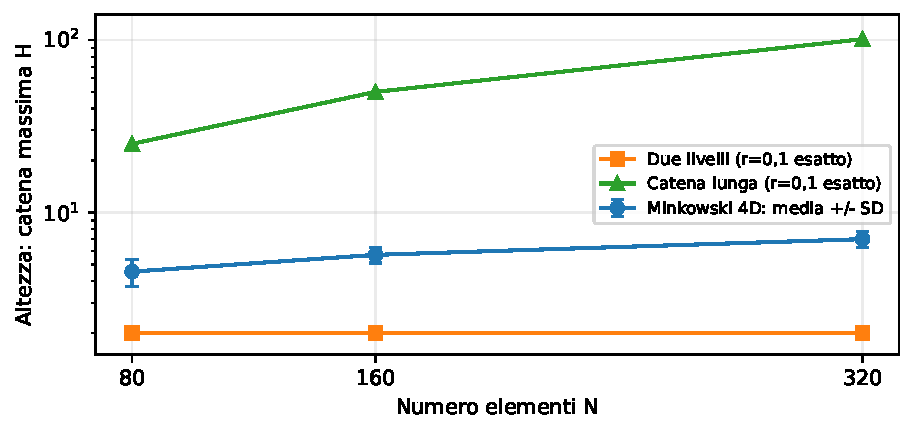
\includegraphics[width=0.9\linewidth,height=7cm,keepaspectratio]{R12BB_G4_HEIGHT.pdf}
\captionof{figure}{Altezza massima: media 4D $\pm$ deviazione standard (64 realizzazioni per taglia), e due ordini avversari con $r=1/10$ identico; asse verticale logaritmico.}
\end{center}
La calibrazione e \emph{positiva e cinematica}: nessun insieme e stato campionato da una distribuzione quantistica QSG, e le frequenze non sono misure quantistiche.

\clearpage
\subsection*{Intervalli, indipendenza algoritmica e decisione fail-closed}
La figura successiva mostra la discriminazione ottenibile con un secondo invariante completamente intrinseco. Il modello a due livelli ha soltanto link ($F_0=1$). Nel modello catena-lunga $F_0=(q-1+\delta)/R_*\to0$. La calibrazione 4D presenta valori intermedi e variabili con $N$; non inferiamo alcuna separazione universale da tre taglie finite.
\begin{center}
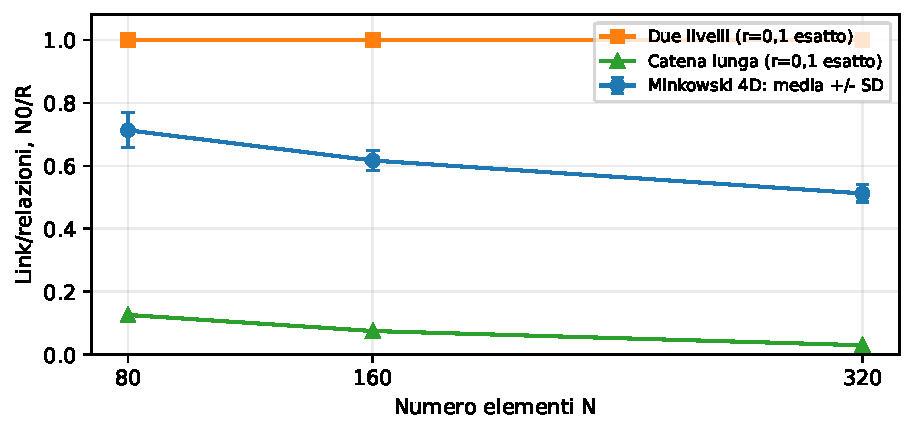
\includegraphics[width=0.9\linewidth,height=7cm,keepaspectratio]{R12BB_G4_LINKS.pdf}
\captionof{figure}{Frazione di link su tutte le relazioni comparabili, $N_0/R$. Media 4D $\pm$ deviazione standard; confronti avversari exact-match rispetto alla sola frazione d'ordine.}
\end{center}
\textbf{Riproducibilita.} La prima implementazione usa maschere di bit e \texttt{bit\_count()} per $|I(x,y)|$; la seconda ricostruisce le stesse quantita dalla matrice intera $M^2$, dove $(M^2)_{xy}=|I(x,y)|$ per ogni coppia comparabile. Concordano sulle sei strutture esatte e su nove realizzazioni 4D holdout ($N=80,160,320$; indici replica $0,7,31$). La seconda implementazione ha rigenerato separatamente gli hash delle matrici di \textbf{288/288} campioni; \textbf{60/60} rietichettature di sei strutture avversarie preservano tutte le grandezze misurate. La chiusura transitiva e controllata esplicitamente, senza dedurla dalle sole cifre.

\textbf{Portata scientifica.} Il test esibisce un \emph{falso positivo geometrico} per una sola statistica e fornisce una suite cinematica autonoma per futuri candidati: $r$, altezza e spettro $N_k$ devono essere analizzati congiuntamente su piu cardinalita. E noto dalla letteratura che la sola dimensione Myrheim--Meyer non equivale a \emph{manifoldlikeness}; gli intervalli sono strumenti aggiuntivi (Glaser--Surya 2013). Le due famiglie avversarie non sono risultati fisici emergenti, e non e dimostrato che la suite sia un criterio sufficiente di immersione in 4D, tanto meno di dinamicita.

\textbf{Divieto di promozione.} I benchmark non selezionano alcuna misura complessa o operatoriale sulle storie, non calcolano l'azione BDG sul proprio path sum, non recuperano Ward/Bianchi, risposta retarded, limite continuo gravitazionale o $H(z)$. Non usiamo il fatto che un evento compaia in una storia supportata come prova di \emph{peso quantistico} su un'algebra covariante infinita. Lo studio chiude \texttt{R12BB-G4 KINEMATIC\_DIAGNOSTIC\_PASS} lasciando \textbf{R12bc NON APERTO; R12as fisico NON AUTORIZZATO; R13 BLOCCATO.}

\textbf{Fonti:} S.~Surya, \emph{Living Reviews in Relativity} (2019), \href{https://doi.org/10.1007/s41114-019-0023-1}{DOI}; L.~Glaser e S.~Surya, \emph{Phys. Rev. D} \textbf{88}, 124026 (2013), \href{https://doi.org/10.1103/PhysRevD.88.124026}{DOI}; D.~Reid, \emph{Phys. Rev. D} \textbf{67}, 024034 (2003), \href{https://doi.org/10.1103/PhysRevD.67.024034}{DOI}.


% === v0.70 R12BB-CV covariant-stem and quantum-amplitude audit; gate R13 blocked ===
\clearpage
\section*{Appendice v0.70 --- R12bb-CV: eventi geometrici covarianti e misura complessa}
\textbf{Quesito.} La diagnostica v0.69 definisce invarianti intrinseci su un \emph{poset finito} ($r,H,N_k$). Ma nella crescita sequenziale un \emph{prefisso} dei primi $n$ elementi dipende dalla scelta della labellatura naturale della storia completa. Il nuovo audit distingue: (i) invarianza dei valori su un poset finito; (ii) invarianza degli \emph{eventi} sulle storie infinite; (iii) misura quantistica assegnata a tali eventi. Nessuna delle tre proprieta implica da sola dinamica geometrica 4D.

\subsection*{Un sollevamento matematico verso eventi covarianti}
Un \emph{stem} $S\subset C$ e un sottoposet finito che contiene tutto il suo passato: $y\in S$ e $x\prec y$ implicano $x\in S$. Per un predicato geometrico $G_n$ definito su ordini \emph{non etichettati} di cardinalita $n$, poniamo
\begin{equation}
 \mathcal E_n(G)=\bigcup_{\substack{[S],\,|S|=n\\G_n(S)}}\operatorname{Stem}(S),\qquad
 \mathcal E_{n,T}(G)=\{\text{entro i primi $T$ nati appare uno stem $S$ con $G_n(S)$}\}.
 \tag{CV.1}
\end{equation}
La prima unione e finita per $n$ fissato (numero finito di poset non etichettati). Ogni \emph{stem event} e unione numerabile di cilindri delle crescite naturali, quindi $\mathcal E_n(G)$ appartiene alla sigma-algebra generata dai cilindri ed e \emph{covariante} sotto ogni rinumerazione naturale della storia completata. I prefissi \emph{entro un taglio $T$} non sono necessariamente covarianti sull'intero spazio infinito. Su ciascuna storia finita, invece, l'esistenza di uno stem e un fatto intrinseco del poset.

\textbf{Lemma esatto.} Un sottoinsieme $S$ di cardinalita $n$ compare come \emph{primo segmento} in qualche ordinamento naturale di $C$ se e solo se $S$ e downward-closed. Il verso ``solo se'' discende dal divieto di nascere prima dei propri antenati; per il viceversa basta concatenare una linearizzazione naturale di $S$ con una di $C\setminus S$. Pertanto
\begin{equation}
 \mathcal E_n(G)\quad\Longleftrightarrow\quad
 \text{esiste una labellatura naturale i cui primi $n$ elementi soddisfano $G_n$}.
 \tag{CV.2}
\end{equation}
Non equivale all'affermazione ``i primi $n$ elementi \emph{della labellatura fissata} soddisfano $G_n$''.

\textbf{Controesempio a sei elementi.} Sia $C$ composto da una sola relazione $a\prec b$ e quattro elementi isolati. Il primo segmento di cinque elementi della labellatura $(a,b,c,d,e,f)$ ha una relazione, dunque $r=1/10$; la labellatura $(a,c,d,e,f,b)$ ha invece $r=0$. Il medesimo poset $C$ possiede comunque uno stem a cinque elementi con $r=1/10$ (per esempio omettendo l'isolato $f$). Questo valore \emph{non e un test 4D}: a $n=5$ una sola relazione e un ordine manifestamente povero di struttura geometrica.

\clearpage
\subsection*{Censimento completo a sei elementi e differenza fra gli eventi}
Per il modello \emph{gia fissato in v0.65}, $t_0=1$, $t_1=i$, $t_k=1$ per $k\ge2$, la crescita complessa e
\begin{equation}
 \begin{aligned}
 T(C,D)&=\frac{\lambda(|D|,m(D))}{\Lambda_{|C|}}, &
 \Lambda_n&=(2^n-n)+in,\\
 \lambda(0,0)&=1, & \lambda(\omega,1)&=2^{\omega-1}-1+i,\\
 \lambda(\omega,m\ge2)&=2^{\omega-m}. &
 \end{aligned}
 \tag{CV.3}
\end{equation}
$D$ e il \emph{precursore downward-closed}, $m(D)$ il numero di suoi elementi massimali. Gli accoppiamenti non sono stati adattati a dati geometrici: sono gli stessi coefficienti del benchmark storico scalare, \emph{non selezionati da una microfisica}. A ogni cardinalita $N$ sommiamo le ampiezze esatte sui cilindri etichettati \emph{disgiunti} che compongono l'evento indicato; riportiamo $\mu(A)=|\nu(A)|^2$, non una frequenza positiva additiva.

Il criterio didattico $G_5$ e \emph{esattamente una relazione su cinque elementi}, ossia $r=1/10$ e $H=2$. Si confrontano il prefisso fissato $P_5$ e l'evento \emph{esiste uno stem} $E_5$ \emph{entro il livello $N$}:
\begin{center}\small
\begin{tabular}{lrrrr}
\toprule
Livello e criterio & strutture $C_N$ & casi ammessi & $\Re\nu$ & $\Im\nu$ \\\midrule
$N=5$, $P_5=E_5$ & 357 & 10 & $0.022058824$ & $-0.025735294$\\
$N=6$, prefisso $P_5$ & 4824 & 240 & $0.022058824$ & $-0.025735294$\\
$N=6$, stem $E_5$ entro $N$ & 4824 & 409 & $0.036013809$ & $-0.041187198$\\
\bottomrule
\end{tabular}
\end{center}
\begin{equation}
 \boxed{\mu_{N=6}(P_5)=0.0011488970588\ldots\,,\qquad
 \mu_{N=6}(E_5\text{ entro }6)=0.0029933796711\ldots}\,.
 \tag{CV.4}
\end{equation}
\textbf{169/4824} storie naturalmente etichettate ammettono uno stem geometrico $G_5$ pur fallendo il prefisso fissato. Questo e un conteggio \emph{delle labellature naturali}, non di 4824 classi di isomorfismo distinte. La differenza nelle ampiezze e un fatto dei \emph{due eventi finiti distinti}; il loro valore non e la misura dell'evento infinito $\mathcal E_5(G_5)$.

\textbf{Due implementazioni esatte.} Il codice primario enumera tutti i downset e genera le strutture, conservando numeratori gaussiani interi e un denominatore comune per livello. L'indipendente genera tutte le matrici di ordine da ciascuno dei $2^{\binom N2}$ DAG orientati secondo l'etichetta, prende la chiusura transitiva e ricava i numeratori contando \emph{sottoinsiemi primitivi} che generano ciascun passato. A $N=1,\ldots,6$ entrambi trovano rispettivamente $1,2,7,40,357,4824$ poset naturalmente etichettati. Concordano in 5285 confronti esatti, inclusi i digest dei 5231 stati cumulativi e le ampiezze di ciascun evento.

\clearpage
\subsection*{Un evento covariante infinito con ampiezza certificata}
Un evento sollevato ai \emph{completamenti infiniti} ammette una misura solo se la misura cilindrica complessa si estende. Per la famiglia specifica di v0.65 questa proprieta e gia garantita dalla maggiorazione uniforme della variazione totale documentata in quel checkpoint, nel solco del criterio di Surya--Zalel (2020). Di conseguenza, per la continuita da sotto della misura complessa sigma-additiva,
\begin{equation}
 \nu(\mathcal E_n(G))=\lim_{T\to\infty}\nu(\mathcal E_{n,T}(G)),\qquad
 \mu(\mathcal E_n(G))=|\nu(\mathcal E_n(G))|^2.
 \tag{CV.5}
\end{equation}
Non si assume additivita di $\mu$. La formula e un ponte \emph{di definizione}, non un calcolo numerico della misura infinita per il filtro $G_5$.

Un caso invece esattamente trattabile e $\mathcal E_2=\operatorname{Stem}(A_2)$, dove $A_2$ e l'anticatena a due elementi: equivale all'esistenza di \emph{almeno due elementi minimi}. Il complemento $O$ e l'evento \emph{originary} (unico minimo). Per la crescita scalare v0.65 l'ampiezza totale delle continuazioni che evitano una nascita con precursore vuoto, al livello $N$, e
\begin{equation}
 \nu_N(O)=\prod_{k=1}^{N-1}\left(1-\frac1{\Lambda_k}\right),\qquad
 \nu(O)=\prod_{k=1}^{\infty}\left(1-\frac1{(2^k-k)+ik}\right),\quad
 \nu(\mathcal E_2)=1-\nu(O).
 \tag{CV.6}
\end{equation}
Un certificato \emph{esatto} in frazioni gaussiane calcola i primi 64 fattori. Per $k\ge4$, $|\Lambda_k|\ge\tfrac34 2^k$ e $|1-1/\Lambda_k|\le1$. La coda obbedisce
\begin{equation}
 S_{64}\le\frac43\,2^{-64},\qquad
 \left|\nu(O)-\nu_{65}(O)\right|\le e^{S_{64}}-1\le\frac{S_{64}}{1-S_{64}}<2^{-63}.
 \tag{CV.7}
\end{equation}
Qui $\nu_{65}$ include i fattori $k=1,\ldots,64$. I valori seguenti hanno quindi errori assoluti minori di $3\cdot2^{-63}$, $5\cdot2^{-63}$ e $8\cdot2^{-63}$ rispettivamente, in ordine:
\begin{equation}
 \begin{aligned}
 \mu(O)&=0.171075812943464\ldots,\\
 \mu(\mathcal E_2)&=0.907552382219550\ldots,\\
 I_2(O,\mathcal E_2)&=\mu(O\cup\mathcal E_2)-\mu(O)-\mu(\mathcal E_2)\\
  &=-0.078628195163014\ldots\ne0.
 \end{aligned}\tag{CV.8}
\end{equation}
$O$ e $\mathcal E_2$ sono complementari, dunque $\mu(O\cup\mathcal E_2)=1$; ciononostante $\mu(O)+\mu(\mathcal E_2)\ne1$. Questo mostra \emph{interferenza quantistica} nel benchmark scalare con eventi covarianti misurabili. Nessuna delle due misure e una probabilita classica.

\clearpage
\subsection*{Audit, non-equivalenze e stato dei gate}
Il certificato dei primi 64 fattori e calcolato sia tramite frazioni gaussiane esatte sia tramite un prodotto complesso separato in aritmetica decimale a 105 cifre. I due metodi concordano oltre $10^{-90}$ sui fattori troncati. Le identita $\nu_N(O)+\nu_N(\mathcal E_2)=1$ sono confermate per tutti i $N=1,\ldots,6$ da 24 confronti esatti; il bound della coda e provato razionalmente. I risultati JSON dei due censimenti e del certificato sono consegnati nel recovery, con programmi autonomi e protocollo validato.

\textbf{Tracciabilita tecnica.} La derivazione del sollevamento a stem e avvenuta esplorativamente prima del congelamento del protocollo di \emph{validazione indipendente} (SHA-256 \texttt{018c2e9c...e262200c3}): non e descritta come previsione preregistrata in fase esplorativa. Nelle prime esecuzioni, in entrambi i programmi, una funzione somma itero due volte su un generatore Python consumabile e produsse una asserzione fallita; il difetto fu corretto materializzando la sequenza prima delle due somme. I fallimenti tecnici sono conservati nella nota di audit, e nessun risultato di quelle esecuzioni e stato promosso a PASS.

\textbf{Tre distinzioni che restano necessarie.}
\begin{enumerate}
 \item Un \emph{poset finito} non dipende dalle sue etichette; un \emph{prefisso temporale} puo invece dipendere dalla labellatura naturale della storia completa. L'evento di stem infinito e covariante; il suo proxy ``gia entro $N$'' resta una costruzione con taglio di nascita.
 \item L'esistenza di una misura complessa sigma-additiva per una dinamica \emph{fissata} autorizza l'assegnazione di $\nu$ e $\mu$ agli eventi covarianti, ma non seleziona quella dinamica fra le infinite misure matematicamente ammesse.
 \item Una statistica geometrica $r=1/10$ ricavata da un ordine microscopico a soli cinque elementi, anche quando appare in uno stem, non certifica \emph{manifold-likeness}, non crea un background 4D e non implica selezione quantistica di quel settore.
\end{enumerate}
\textbf{Decisione.} Il gate \texttt{R12BB-CV} passa come \emph{bridge matematico della measurabilita covariante} e come calcolo esatto di interferenza sul benchmark scalare storico; \emph{non} e una dinamica quantistica gravitazionale selezionata. Non abbiamo derivato un funzionale operatoriale QBC non commutativo, un'azione BDG incorporata nella misura, un settore tensoriale gravitazionale 4D conservato, una risposta retarded o una legge $H(z)$ autonoma. \textbf{R12bc NON APERTO; R12as fisico NON AUTORIZZATO; R13 BLOCCATO.}

\textbf{Letteratura:} G.~Brightwell, F.~Dowker, R.~S.~Garcia, J.~Henson, R.~D.~Sorkin, \emph{``Observables'' in causal set cosmology}, \emph{Phys. Rev. D} \textbf{67}, 084031 (2003), \href{https://doi.org/10.1103/PhysRevD.67.084031}{DOI}; S.~Surya e S.~Zalel, \emph{A criterion for covariance in complex sequential growth models}, \emph{Class. Quantum Grav.} \textbf{37}, 195030 (2020), \href{https://doi.org/10.1088/1361-6382/ab987f}{DOI}; S.~Surya, \emph{The causal set approach to quantum gravity}, \emph{Living Rev. Relativ.} (2019), \href{https://doi.org/10.1007/s41114-019-0023-1}{DOI}.


% === v0.71 R12BB-FI finite-stem interference and cutoff covariance audit, physical gates remain blocked ===
\clearpage
\section*{Appendice v0.71 --- R12bb-FI: interferenza e tagli finiti degli stem geometrici}
\textbf{Quesito e preregistrazione.} L'appendice v0.70 ha reso misurabile un evento geometrico covariante di \emph{stem}, senza calcolarne l'ampiezza nel limite delle storie infinite. Qui si applica \emph{senza alcuna nuova scelta di parametri} il modello di crescita complessa storico di v0.65, $t_0=1$, $t_1=i$, $t_k=1$ ($k\ge2$), ad un solo livello aggiuntivo: da $N=6$ a $N=7$. Protocollo di audit congelato prima del censimento v0.71, SHA-256 \texttt{c59f2fbfde40...53231392}. L'ipotesi non prescrive il segno del cambiamento di misura.

Come nella v0.70, $G_5(S)$ significa precisamente: $|S|=5$ e una sola relazione d'ordine stretta su dieci coppie; $r(S)=1/10$. Si tratta di un \emph{filtro didattico}, non di un certificato di spazio-tempo quadridimensionale. Per una storia naturalmente etichettata poniamo
\begin{equation}
\begin{aligned}
A_6&=\{\exists\;5\text{-stem }S\subseteq C_6:G_5(S)\},\\
B_7&=\{\neg A_6,\;\exists\;5\text{-stem }S\subseteq C_7:G_5(S)\},\\
A_7&=A_6\,\dot\cup\,B_7.
\end{aligned}\tag{FI.1}
\end{equation}
Nella terza riga gli eventi sono interpretati sullo \emph{stesso} spazio di storie etichettate di lunghezza sette; $A_6$ e sollevato a $N=7$ tramite unione dei cilindri figli. Sono \emph{tagli finiti}: $A_6$ e $B_7$ non sono, in generale, invarianti sotto tutte le labellature naturali di uno stesso causal set.

\textbf{Censimento completo.} Da tutti i 4\,824 poset naturalmente etichettati a sei elementi si enumerano gli ideal/downset e tutte le loro estensioni: risultano \textbf{96\,428} poset naturalmente etichettati a sette elementi, senza duplicati. La partizione esatta e
\begin{center}\small
\begin{tabular}{lrr}
\toprule
Evento sui sette elementi & Numero di stati etichettati & Definizione \\\midrule
$A_6$ gia vero alla sesta nascita & 12\,707 & \emph{old}\\
$B_7$ compare per la prima volta alla settima & 2\,987 & \emph{new}\\
$\neg A_7$ (nessuno stem $G_5$) & 80\,734 & \emph{never}\\\midrule
Totale & 96\,428 & Partizione disgiunta\\
$P_5$ (solo prefisso iniziale fissato) & 7\,380 & Controllo separato\\
\bottomrule
\end{tabular}
\end{center}
Le cifre contano storie naturalmente etichettate, \emph{non} classi di poset non etichettati e \emph{non} probabilita. Il prefisso $P_5$ mantiene per consistenza cilindrica la propria ampiezza tra $N=5,6,7$.

\clearpage
\subsection*{Ampiezze esatte e interferenza tra incrementi disgiunti}
Ogni storia naturale al livello $N$ conserva un numeratore intero gaussiano su un denominatore comune $D_N=\prod_{k=1}^{N-1}[(2^k-k)+ik]$. Le ampiezze dei tre gruppi v0.71, ridotte a frazioni gaussiane, sono
\begin{equation}
\begin{aligned}
\nu(A_6)&=\frac{3693}{102544}-i\frac{8447}{205088},\\
\nu(B_7)&=\frac{756569}{102544000}-i\frac{197077}{25636000},\\
\nu(A_7)&=\frac{4449569}{102544000}-i\frac{156619}{3204500}\\
&=\nu(A_6)+\nu(B_7).
\end{aligned}\tag{FI.2}
\end{equation}
Definendo $\mu(E)=|\nu(E)|^2$ e $I_2(A,B)=2\operatorname{Re}[\nu(A)\overline{\nu(B)}]$, si ha \emph{esattamente}
\begin{equation}
\begin{aligned}
\mu(A_6)&=\frac{19645}{6562816}=0.002993379671\ldots,\\
\mu(B_7)&=\frac{25333181}{223135744000}=0.000113532599\ldots,\\
I_2(A_6,B_7)&=\frac{3248503}{2789196800}=0.001164673285\ldots,\\
\mu(A_7)&=\frac{953143421}{223135744000}=0.004271585556\ldots.
\end{aligned}\tag{FI.3}
\end{equation}
Pertanto il cambiamento $\Delta\mu=\mu(A_7)-\mu(A_6)$ non coincide con la misura quantistica delle sole storie nuove:
\begin{equation}
\begin{aligned}
\Delta\mu&=\frac{285213421}{223135744000}=0.001278205884\ldots\\
 &=\mu(B_7)+I_2(A_6,B_7),\\
\frac{I_2(A_6,B_7)}{\Delta\mu}&=\frac{259880240}{285213421}=91.1178\ldots\%.
\end{aligned}\tag{FI.4}
\end{equation}
In \emph{questa} decomposizione a taglio di nascita, la maggior parte dell'incremento e' un termine di interferenza. Non e' una frequenza, una probabilita condizionata, o una ``frazione dell'universo'' e non e' un numero fisico indipendente dalle labellature. Sui tre tagli disponibili $N=5,6,7$ la misura cresce, ma il protocollo non autorizza alcuna estrapolazione monotona a $N\to\infty$. La sigma-additivita della misura complessa riguarda $\nu$ sugli eventi misurabili, \emph{non} l'additivita o la monotonicita di $\mu$.

\clearpage
\subsection*{Testimone esplicito di dipendenza dalla nascita e audit indipendente}
\textbf{Un medesimo ordine finito, due decomposizioni differenti.} Si consideri il causal set di sette elementi avente \emph{un'unica} relazione non banale e cinque elementi isolati. Una sua labellatura naturale ha come unica relazione $5\prec6$; un'altra, ottenuta scambiando le due ultime nascite causalmente indipendenti, ha come unica relazione $5\prec7$. Nel primo caso uno stem con $G_5$ era gia' presente entro sei nascite; nel secondo non lo era e compare al settimo elemento. I due poset di cardinalita sette sono isomorfi, ed entrambi soddisfano $A_7$. Dunque
\begin{equation}
 \boxed{A_7\text{ e' un invariante del poset finito, mentre }A_6,B_7
 \text{ dipendono dal prefisso scelto.}}\tag{FI.5}
\end{equation}
L'\emph{interferenza 91.1178\%} in (FI.4) e' un risultato numerico esatto del partizionamento adottato, \textbf{non un osservabile covariante fisico}. E' un esempio del problema gia' distinto teoricamente nella v0.70: solo l'evento di stem sull'intera storia infinita, unione sui tagli, e' covariante. Il presente audit non calcola $\nu(\mathcal E_5)$ ne' $\mu(\mathcal E_5)$ al limite infinito.

\textbf{Due algoritmi indipendenti.} Il primo estende con downset le 4\,824 storie $N=6$ verificate nel parent e mantiene i numeratori interi gaussiani. Il secondo rigenera autonomamente gli $N=6$ come chiusure di tutti i $2^{15}$ grafi orientati upper-triangular, determina le ampiezze di \emph{ogni} storia $N=7$ contando tutti i sottoinsiemi primitivi delle nascite precedenti e valuta gli stem per cancellazione di due elementi finali. I risultati coincidono su \textbf{96\,428/96\,428} numeratori esatti e su \textbf{289\,284/289\,284} indicatori (old, stem by7, prefisso), oltre a conteggi, somme gaussiane, normalizzazione e identita d'interferenza razionali. Un testimone delle due labellature e' documentato a parte, dopo il censimento, come controllo secondario esplorativo.

\textbf{Limiti e stato dei gate.} R12bb-FI e' un audit esatto di \emph{cutoff} e non seleziona una misura fisica gravitazionale. La nozione geometrica $G_5$ rimane debole; la misura scalare complessa resta un benchmark non derivato dalla microfisica. Nessuna causalita di Bell operatoriale non commutativa, nessuna azione BDG accoppiata, nessuna geometria dinamica 4D, nessuna conservazione gravitazionale o legge cosmologica $H(z)$ e' stata ottenuta. \textbf{R12bc NON APERTO; R12as fisico NON AUTORIZZATO; R13 BLOCCATO.}

\textbf{Fonti concettuali:} G.~Brightwell et al., \emph{``Observables'' in causal set cosmology}, Phys.~Rev.~D \textbf{67}, 084031 (2003); S.~Surya e S.~Zalel, \emph{A criterion for covariance in complex sequential growth models}, Class.~Quantum Grav.~\textbf{37}, 195030 (2020). Le identita finite FI.2--FI.5 sono verifiche del presente progetto, non teoremi nuovi attribuiti a tali pubblicazioni.


% === v0.72 R12BB-RG null rogues and analytic late-stem bounds; R12bc and R13 blocked ===
\clearpage
\section*{Appendice v0.72 --- R12bb-RG: rogue nulli e controllo di cutoff per gli stem}
\textbf{Oggetto e provenienza.} Questa appendice riprende \emph{senza alcuna modifica} la crescita complessa scalare v0.65--v0.71, $t_0=1$, $t_1=i$, $t_k=1$ per $k\ge2$. Indaghiamo se le storie \emph{rogue} possano ostacolare la completezza degli osservabili costruiti dagli stem. Il problema insiemistico e la caratterizzazione dei rogue sono studiati in Brightwell et al.~(2003); l'estendibilita delle misure complesse e discussa da Surya e Zalel (2020). La stima quantitativa seguente e una derivazione del \emph{benchmark fissato}, non una scelta microfisica. La derivazione e stata esplorativa; il protocollo di audit indipendente e stato congelato solo successivamente (SHA-256 \texttt{422f160f490c...ba629}).

Per un ordine causale naturalmente etichettato $C_n$, sia $D$ un suo \emph{downset}, $w=|D|$, $m=|\operatorname{Max}(D)|$. Se $\downarrow X$ denota la chiusura causale inferiore di $X$, allora
\begin{equation}
\begin{split}
\Lambda_n&=\sum_{k=0}^n\binom nk t_k=2^n-n+in,\\
\lambda(D)&=\sum_{k=m}^{w}\binom{w-m}{k-m}t_k
 =\sum_{\substack{X\subseteq C_n\\\downarrow X=D}}t_{|X|},\qquad
T(C_n,D)=\frac{\lambda(D)}{\Lambda_n}.
\end{split}\tag{RG.1}
\end{equation}
La seconda uguaglianza conta gli insiemi primitivi che producono lo stesso passato. Siccome $|t_k|=1$,
\begin{equation}
\sum_{D\text{ downset}}|\lambda(D)|\le
\sum_{X\subseteq C_n}|t_{|X|}|=2^n.
\tag{RG.2}
\end{equation}
Sia $\nu$ la misura complessa delle storie infinite e $|\nu|$ la sua \emph{variazione totale positiva}. Al livello $n$ il maggiorante di norma e $c_n=2^n/|\Lambda_n|$. Per $n\ge2$, $x_n=n/2^n\le1/2$, quindi
\begin{equation}
\log c_n\le-\log(1-x_n)\le 2x_n,\quad
\sum_{n\ge2}\frac n{2^n}=\frac32,\quad c_1=\sqrt2.
\tag{RG.3}
\end{equation}
Pertanto, includendo tutte le future continuazioni delle storie cilindriche,
\begin{equation}
\boxed{\ |\nu|(\Omega)\le \prod_{n\ge0}c_n\le \sqrt2\,e^3<32.\ }
\tag{RG.4}
\end{equation}
La disuguaglianza finale ammette un certificato razionale, $\sqrt2<3/2$, $e^3<21$ mediante serie di Taylor e limite geometrico della coda. La consistenza cilindrica e questa norma uniforme giustificano la misura complessa sigma-additiva sul limite proiettivo compatto, con variazione totale finita. \textbf{Non e una probabilita classica}: $\mu(E)=|\nu(E)|^2$ e la misura quantistica rank-one.

\clearpage
\subsection*{Nascite con passato limitato, livelli finiti e algebra covariante}
Sia $F_{n,K}$ l'evento che il nuovo elemento, alla nascita $n\to n+1$, abbia al piu $K$ antenati. Se $|\downarrow X|\le K$, necessariamente $|X|\le K$. Usando (RG.1)--(RG.4), anche \emph{dopo tutte le continuazioni future}, per $n\ge2$ otteniamo
\begin{equation}
\boxed{\quad |\nu|(F_{n,K})\le
32\,\frac{\sum_{j=0}^{K}\binom nj}{|\Lambda_n|}
\le \frac{64}{2^n}\sum_{j=0}^{K}\binom nj.\quad}
\tag{RG.5}
\end{equation}
Per ogni $K$ fissato la serie dei maggioranti e sommabile; applicando Borel--Cantelli alla \emph{misura positiva} $|\nu|$ (indipendenza non richiesta),
\begin{equation}
|\nu|\bigl(\limsup_{n\to\infty}F_{n,K}\bigr)=0,
\qquad |\nu|\left(\bigcup_{K=0}^{\infty}\limsup_n F_{n,K}\right)=0.
\tag{RG.6}
\end{equation}
\textbf{Esclusione dei livelli infiniti.} In un causal set \emph{past-finite} ogni elemento ha livello finito. Se esistesse un livello con infiniti elementi, scegliamo il primo, $\ell$. I livelli precedenti avrebbero in tutto un numero finito $K$ di elementi. Il passato di ciascun elemento del livello $\ell$ sarebbe contenuto in quei $K$ elementi: avremmo infinite nascite appartenenti a $F_{n,K}$, contraddicendo (RG.6) fuori da un insieme nullo.
\begin{equation}
|\nu|(\{\text{esiste un livello causale infinito}\})=0.
\tag{RG.7}
\end{equation}
Brightwell, Dowker, Garc\'ia, Henson e Sorkin hanno caratterizzato l'insieme $\Theta$ dei \emph{rogue} come le storie contenenti un livello con infiniti elementi \emph{non massimali}; dunque $\Theta$ e incluso nell'evento di (RG.7):
\begin{equation}
\boxed{\quad |\nu|(\Theta)=0,\quad\nu(\Theta)=0,\quad\mu(\Theta)=0.\quad}
\tag{RG.8}
\end{equation}
La loro proposizione insiemistica afferma che per ogni evento covariante Borel $A$ esiste un evento $B$ nell'algebra sigma generata dagli stem tale che $A\triangle B\subseteq\Theta$. Quindi $\nu(A)=\nu(B)$ e $\mu(A)=\mu(B)$. Per $D(A,C)=\nu(A)\overline{\nu(C)}$, anche $D(A,C)=D(B,C)$. E \emph{completezza modulo insiemi nulli}, non identita letterale degli eventi, e riguarda soltanto la misura scalare fissata.

\clearpage
\subsection*{Errore rigoroso per la comparsa tardiva di stem finiti}
Sia $E_G$ l'evento covariante infinito ``esiste uno stem con proprieta $G$'', dove gli stem hanno cardinalita $h$. Sia $E_{G,N}$ il proxy ``gia comparso entro le prime $N$ nascite''. Se uno stem appare per la prima volta dopo $N$, la nuova nascita ne e necessariamente un elemento e ha al massimo $h-1$ predecessori. Pertanto
\begin{equation}
\begin{split}
|\nu(E_G)-\nu(E_{G,N})|&\le |\nu|(E_G\setminus E_{G,N})\\
&\le U(N,h-1),\quad
U(N,K)=64\sum_{n=N}^{\infty}2^{-n}\sum_{j=0}^{K}\binom nj.
\end{split}\tag{RG.9}
\end{equation}
L'identita geometrico-binomiale
\begin{equation}
\sum_{n=N}^{\infty}\binom nj2^{-n}=
2^{1-N}\sum_{k=0}^{j}\binom Nk
\tag{RG.10}
\end{equation}
fornisce il \emph{certificato esatto, razionale}, non una stima da fitting:
\begin{equation}
\boxed{\quad U(N,K)=\frac{128}{2^N}
\sum_{k=0}^{K}(K+1-k)\binom Nk.\quad}
\tag{RG.11}
\end{equation}
Per il filtro illustrativo $G_5$ della v0.70--v0.71 (cinque elementi e \emph{una sola} relazione, $r=1/10$, non certificazione di geometria 4D) e $K=4$:
\begin{center}\small
\begin{tabular}{rll}
\toprule
Taglio $N$ & $U(N,4)$ \emph{esatto} & Valore decimale \\\midrule
7 & $201$ & non informativo \\
24 & $15603/131072$ & $0.1190414429$ \\
32 & $47501/33554432$ & $0.00141564012$ \\
48 & $232753/2199023255552$ & $1.05843810\times10^{-7}$ \\
64 & $725013/144115188075855872$ & $5.03078829\times10^{-12}$ \\
\bottomrule
\end{tabular}
\end{center}
\textbf{Questo limite non fornisce il valore di $\nu(E_{G_5})$.} In particolare il risultato esatto $N=7$ della v0.71 non permette un'inferenza numerica utile sulla misura dell'evento infinito. Per sfruttare un taglio $N=32$ occorrerebbe prima calcolare $\nu(E_{G_5,32})$ con un metodo non enumerativo, attualmente assente. Non e lecito convertire automaticamente (RG.11) in monotonicita o additivita di $\mu$.

\clearpage
\subsection*{Audit indipendente, fonti e stato dei gate}
\textbf{Due codici distinti con parametri invariati.} Il primo ricostruisce gli ordini fino a sei elementi dai prefissi dello storico N7 v0.71, enumera gli ideal/downset e usa la formula chiusa di $\lambda(D)$ basata su $|D|$ e sui suoi massimali. Il secondo rigenera tutti gli ordini tramite chiusura di tutti i grafi triangolari orientati e conta direttamente ogni sottoinsieme primitivo $X$; non importa le funzioni del primo. Il confronto e \emph{voce per voce}, non soltanto tramite hash.
\begin{center}\small
\begin{tabular}{lr}
\toprule
Verifica esatta & Esito \\\midrule
Ordini causali N=0--6 (incluso vuoto) & $5\,232/5\,232$ PASS\\
Coefficienti Gaussiani / downset, confronto integrale & $101\,659/101\,659$ PASS\\
Disuguaglianze per passato $K\le4$ & $26\,142/26\,142$ PASS\\
Disuguaglianze Gaussiane di triangolo & $101\,659/101\,659$ PASS\\
Identita indipendenti delle code razionali & $14/14$ PASS\\
\bottomrule
\end{tabular}
\end{center}
La verifica di $e^3<21$ e documentata mediante intervalli razionali. Il risultato infinito discende dalla dimostrazione, non dal censimento $N\le6$. La scelta del teorema e stata \emph{esplorativa}; solo la verifica matematica indipendente e stata congelata prima dell'esecuzione.

\textbf{Limiti scientifici.} L'assenza, quasi ovunque per $|\nu|$, degli \emph{rogue} dimostra che gli stem rappresentano gli eventi covarianti del \emph{benchmark complesso specifico} modulo insiemi nulli. Non seleziona fra le misure possibili, non dimostra una legge gravitazionale, non incorpora l'azione BDG nella crescita, non crea causalita di Bell operatoriale non commutativa, geometria dinamica 4D o una legge autonoma $H(z)$. $|\nu|$ e una misura ausiliaria di variazione totale: non e una probabilita fisica predittiva.

\textbf{Decisione R12bb-RG.} Supera l'audit come limite rigoroso per rogue e comparsa tardiva degli stem; nessun nuovo gate fisico e sbloccato. \textbf{R12bc NON APERTO; R12as fisico NON AUTORIZZATO; R13 BLOCCATO.}

\textbf{Fonti:} G.~Brightwell, F.~Dowker, R.~S.~Garc\'ia, J.~Henson, R.~D.~Sorkin, ``Observables'' in causal set cosmology, \emph{Phys. Rev. D} \textbf{67}, 084031 (2003), \href{https://doi.org/10.1103/PhysRevD.67.084031}{DOI}, in particolare Lemmi~1--3 e Proposizione~2; S.~Surya, S.~Zalel, \emph{A Criterion for Covariance in Complex Sequential Growth Models}, \emph{Class. Quantum Grav.} \textbf{37}, 195030 (2020), \href{https://doi.org/10.1088/1361-6382/ab987f}{DOI}.


% === v0.73 R12BB-PT percolation-equivalence and covariant geometric obstruction, R13 still blocked ===
\clearpage
\section*{Appendice v0.73 --- R12bb-PT: dominazione classica ed esclusione di stem a bassa frazione ordinata}
\textbf{Oggetto e limiti.} Riprendiamo il medesimo benchmark scalare complesso delle v0.65--v0.72, $t_0=1$, $t_1=i$, $t_k=1$ per $k\ge2$. Deriviamo una relazione di Radon--Nikodym con la \emph{percolazione transitiva classica} a $p=1/2$ e un conseguente test geometrico covariante. \emph{Non} scegliamo una misura quantistica gravitazionale. La derivazione e esplorativa, mentre il protocollo di validazione indipendente e congelato dopo l'idea e prima dei test (SHA-256 \texttt{e3e7e3d0ccf5...edbf81}).

\textbf{Conteggio dei sottoinsiemi primitivi.} Per un downset $D$ di uno stato $C_n$, poniamo $w=|D|$ e $m=|\operatorname{Max}(D)|$. Nella percolazione $p=1/2$, un sottoinsieme diretto $X\subset C_n$ e scelto uniformemente e produce $D=\downarrow X$; il numero di $X$ con quella chiusura e $2^{w-m}$. In particolare,
\begin{equation}
P_n(D)=\frac{2^{w-m}}{2^n},\qquad
\lambda_i(D)=2^{w-m}+(i-1)\mathbf{1}_{\{m=1\}},\qquad
\Lambda_n=2^n-n+in.
\tag{PT.1}
\end{equation}
La correzione $i-1$ compare per tutti gli \emph{ideali principali} $m=1$, non soltanto quando $w=1$. Il rapporto con la transizione classica e
\begin{equation}
q(D)=\frac{\lambda_i(D)}{2^{w-m}}=\begin{cases}
(1-u)+iu,\quad u=2^{-(w-1)},&m=1,\\
1,&m\ne1.
\end{cases}\quad 0<|q(D)|\le1.
\tag{PT.2}
\end{equation}
Quando $w=2,m=1$ si ha $\lambda_i=1+i$ contro $\lambda_P=2$, dunque $|q|=1/\sqrt2$: \textbf{non e una semplice rotazione di fase}. Tutti i fattori sono non nulli.

\textbf{Martingala di Radon--Nikodym.} Sulla sigma-algebra delle storie naturalmente etichettate, sia $P$ la probabilita della percolazione e $\nu$ la misura complessa estesa della v0.72. Sui cilindri $C_n$,
\begin{equation}
L_n=\frac{\nu(C_n)}{P(C_n)}=
\prod_{j<n}\frac{2^j}{\Lambda_j}\prod_{j<n}q(D_j),\qquad
\mathbb{E}_{P}[L_{n+1}\mid\mathcal F_n]=L_n.
\tag{PT.3}
\end{equation}
Per (PT.2), $|L_n|\le B=\prod_{j\ge0}2^j/|\Lambda_j|\le\sqrt2 e^3<32$, riprendendo il limite gia provato nella v0.72. La martingala e limitata, percio converge in $L^1(P)$ e quasi sicuramente a $L_\infty$; segue $\nu(E)=\int_E L_\infty\,dP$ per ogni evento Borel. Il valore numerico diagnostico $B\simeq5.030017968$ \emph{non} e $|\nu|(\Omega)$.

\clearpage
\subsection*{Equivalenza degli insiemi nulli e misura quantistica}
Il prodotto $\prod_j2^j/\Lambda_j$ e non nullo, dato che nessun denominatore si annulla e $\sum_j|\Lambda_j/2^j-1|=\sqrt2\sum_j j2^{-j}=2\sqrt2<\infty$. Per i $q(D_j)$, sia $X_j$ il sottoinsieme diretto selezionato al tempo $j$. Poiche $|\downarrow X_j|\ge|X_j|$,
\begin{equation}
\begin{split}
|q(D_j)-1|&\le2\sqrt2\,2^{-|X_j|}\mathbf{1}_{X_j\ne\varnothing},\\
\sum_{j\ge1}\mathbb E_P|q(D_j)-1|&\le2\sqrt2\sum_{j\ge1}\left[(3/4)^j-(1/2)^j\right]=4\sqrt2<6.
\end{split}\tag{PT.4}
\end{equation}
Quindi $\sum_j|q(D_j)-1|<\infty$ quasi sicuramente. Essendo ciascun $q(D_j)$ diverso da zero, il prodotto infinito converge \emph{a un valore non nullo}. Di conseguenza $0<|L_\infty|\le B$ quasi sicuramente e
\begin{equation}
\boxed{\qquad|\nu|(E)=\int_E|L_\infty|\,dP\le B P(E),\quad
P(E)=0\ \Longleftrightarrow\ |\nu|(E)=0.\qquad}
\tag{PT.5}
\end{equation}
L'equivalenza degli insiemi nulli vale fra $P$ e \emph{variazione totale positiva} $|\nu|$, \textbf{non} fra $P$ e la misura quantistica $\mu(E)=|\nu(E)|^2$. Un evento di $P$ positiva puo comunque avere $\nu(E)=0$ per interferenza; viceversa $P(E)=0$ implica $\mu(E)=0$.

\textbf{Audit esatto.} Due programmi separati verificano il modello su tutte le 5.232 storie naturalmente etichettate fino a sei elementi, compreso l'ordine vuoto. Il primo usa il ledger storico della v0.72; il secondo rigenera \emph{tutti} i grafi triangolari orientati, ne calcola la chiusura transitiva e conta direttamente ogni sottoinsieme primitivo. Entrambi concordano, numero razionale per numero razionale, su 101.659 transizioni e sulle 5.232 ampiezze e rapporti a $P$. Risultano 30.915 downset con un solo massimo, dei quali 17.177 presentano una contrazione stretta del modulo. L'impronta dell'intero ledger di storie coincide: \texttt{17c1f9230ce44bda...baeddbe72}.

\textbf{Significato.} La deformazione complessa puo cambiare i moduli delle ampiezze dei singoli cilindri e produrre interferenza, ma \emph{non modifica gli insiemi nulli di variazione totale} della percolazione $p=1/2$. Questo e un vincolo negativo sul benchmark esistente, non un principio microfisico che determini i coefficienti.

\clearpage
\subsection*{Un limite geometrico valido per tutti gli stem grandi}
Per la percolazione $p=1/2$, siano $i<j$ due indici naturali, con $d=j-i$. Se $i$ non precede causalmente $j$, deve mancare sia l'arco diretto $i\to j$, sia ogni cammino in due salti $i\to k\to j$, $i<k<j$. Le scelte di archi sono indipendenti, dunque
\begin{equation}
P(i\not\prec j)\le\frac12\left(\frac34\right)^{d-1}.
\tag{PT.6}
\end{equation}
Scegliamo $\ell(j)=1+\lceil12\log_2j\rceil$ per $j\ge2$. Per unione degli eventi e per $(3/4)^3=27/64<1/2$,
\begin{equation}
P\left(\exists i\le j-\ell(j):\ i\not\prec j\right)
\le2(3/4)^{\ell(j)-1}\le 2j^{-4}.
\tag{PT.7}
\end{equation}
La serie converge; Borel--Cantelli assicura che, quasi sicuramente, per tutti i $j$ sufficientemente grandi ogni $i\le j-\ell(j)$ precede $j$. Questa e una proprieta dimostrata sulla crescita etichettata, ma produce una conclusione \emph{intrinseca}.

Infatti sia $S$ un \emph{qualsiasi} stem finito di $n$ elementi e $J$ la piu grande etichetta naturale presente in $S$. Siccome lo stem contiene tutto il passato dell'elemento $J$, esso include almeno i $J-\ell(J)$ elementi anteriori garantiti da (PT.7). Per grandi $J$, $\ell(J)\le J/2$, quindi $J\le2n$. Una coppia incomparabile in $S$ con indice maggiore $j$ deve avere distanza fra etichette inferiore a $\ell(j)$, salvo eccezioni iniziali finite. Per \emph{ogni} stem di $n$ elementi,
\begin{equation}
\#\{\text{coppie incomparabili in }S\}\le O(n\log n),
\qquad 1-r(S)=O\!\left(\frac{\log n}{n}\right),
\tag{PT.8}
\end{equation}
con costante dipendente dalla storia ma \emph{uniforme su tutti gli stem dello stesso ordine}. Si ha quindi
\begin{equation}
\boxed{\ P\text{-q.s.}:\quad\lim_{N\to\infty}
\sup_{\substack{S\text{ stem finito}\\ |S|\ge N}}(1-r(S))=0.\ }
\tag{PT.9}
\end{equation}
L'enunciato non dipende dalla scelta di etichettatura naturale; questa e soltanto uno strumento della dimostrazione. Per ogni $\rho<1$ fisso l'evento \emph{covariante e Borel}, costruito dalla sigma-algebra degli stem,
\begin{equation}
F_\rho=\left\{\text{esistono stem arbitrariamente grandi con }r(S)\le\rho\right\},
\quad\boxed{\ |\nu|(F_\rho)=\nu(F_\rho)=\mu(F_\rho)=0.\ }
\tag{PT.10}
\end{equation}
\clearpage
\subsection*{Confronto diagnostico, replicabilita e gate fisici}
Per un diamante piatto di Minkowski 4D il riferimento Myrheim--Meyer sulla frazione di coppie ordinate e $r_4=1/10$. Ne segue che il benchmark complesso fissato \emph{non supporta con misura quantistica non nulla} l'evento covariante che richieda stem arbitrariamente grandi con $r\le\rho$ per un $\rho<1$ fissato, incluso $\rho=1/5$ che contiene il riferimento $1/10$. \textbf{Questa non e un'esclusione universale della manifold-likeness 4D}: un solo indicatore, e persino gli stem, non caratterizzano ogni geometria o limite continuo possibile.

\begin{figure}[h!]
\centering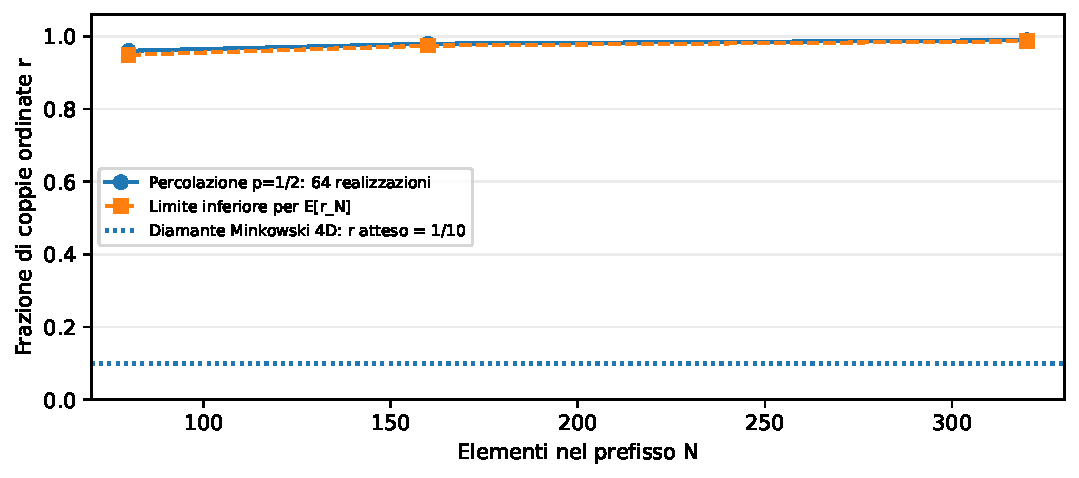
\includegraphics[width=.90\linewidth]{R12BB_PT_ORDERING_FRACTION.pdf}
\caption{Sanity check \emph{non dimostrativo}: 64 percolazioni con seed 202610110073, ciascuna fino a 320 elementi; media della frazione ordinata ai tre tagli. La curva analitica inferiore riguarda $\mathbb{E}[r_N]$, non ogni singola storia. $r_4=1/10$ e il riferimento per diamanti di Minkowski piatto 4D, non un parametro adattato.}
\end{figure}

\textbf{Certificati e replay.} Sono passati 5.232/5.232 confronti delle ampiezze, 101.659/101.659 coefficienti di transizione in \emph{due} algoritmi e 8/8 enumerazioni razionali della probabilita di mancanza di cammini a lunghezza uno o due. Sono stati controllati esattamente 128 fattori $q(w)$; la somma delle probabilita di eccezioni dopo l'indice $512$ e limitata superiormente da
\begin{equation}
\sum_{j=512}^{\infty}2j^{-4}\le\frac{2}{3\cdot511^3}<5\cdot10^{-9}.
\tag{PT.11}
\end{equation}
I valori simulati medi sono $r_{80}=0.960651$, $r_{160}=0.980114$ e $r_{320}=0.989915$. La prova di (PT.9)--(PT.10) discende da (PT.6)--(PT.8), \emph{non} dalle simulazioni. Discovery analitica prima del freeze di validazione, esplicitamente dichiarata.

\textbf{Decisione R12bb-PT:} test matematico negativo sostanziale per il benchmark CSG complesso. Non selezionata la misura fisica; non incorporata l'azione BDG; non derivati QBC operatoriale non commutativa, gravita dinamica 4D, Ward/Bianchi, risposta causale o legge autonoma $H(z)$. \textbf{R12bc NON APERTO; R12as fisico NON AUTORIZZATO; R13 BLOCCATO.}

\textbf{Fonti:} Rideout e Sorkin, \emph{Classical sequential growth dynamics for causal sets}, PRD~61, 024002 (1999), DOI \href{https://doi.org/10.1103/PhysRevD.61.024002}{10.1103/PhysRevD.61.024002}; Bollob\'as e Brightwell, \emph{The Structure of Random Graph Orders}, \href{https://doi.org/10.1137/S0895480194281215}{DOI}; Surya, \emph{The causal set approach to quantum gravity}, LRR~22, 5 (2019), \href{https://doi.org/10.1007/s41114-019-0023-1}{DOI}; Surya e Zalel (2020), \href{https://doi.org/10.1088/1361-6382/ab987f}{DOI}. La prova PT.1--PT.11 appartiene a questo audit del modello fissato.

\clearpage
\section*{Appendice v0.74 --- R12bb-LI: saturazione degli intervalli causali finiti}
\textbf{Motivazione e separazione dei domini.} La v0.73 ha dimostrato che, nella percolazione transitiva $P_{1/2}$, gli \emph{stem} arbitrariamente grandi hanno frazione di coppie ordinate che tende uniformemente a uno; la misura complessa fissata $\nu$ con $t_0=1,t_1=i,t_k=1$ ($k\ge2$) ha gli stessi insiemi nulli della variazione totale positiva di $P_{1/2}$. Qui studiamo invece gli \emph{intervalli causali aperti} $I(x,y)=\{z:x\prec z\prec y\}$, senza cambiare alcun accoppiamento. Uno stem e un insieme chiuso verso il passato; un intervallo fra due estremi \emph{non} deve contenere tutto il passato degli estremi.

\textbf{Costruzione esatta.} Fissiamo un poset non vuoto $Q$ di $n$ elementi con una sua etichettatura naturale. Scriviamo $R(Q)$ per il numero di coppie comparabili, $c(Q)$ per il numero di relazioni di copertura, e $a(Q),b(Q)$ per i numeri di elementi rispettivamente minimi e massimi. Consideriamo un blocco di $n+2$ nascite consecutive, i cui primi e ultimi elementi siano $x$ e $y$. Per ottenere $I(x,y)\simeq Q$, gli archi primitivi interni devono contenere esattamente le $c(Q)$ coperture, mentre gli altri $R(Q)-c(Q)$ archi tra coppie comparabili sono facoltativi. Occorre inoltre collegare direttamente $x$ a ogni elemento minimo e ogni elemento massimo a $y$; i collegamenti agli altri elementi sono liberi, come l'arco $x\to y$. Tutte le scelte primitive sono Bernoulli indipendenti con parametro storico $p=1/2$.

Pertanto, su $2^{\binom{n+2}{2}}$ assegnazioni primitive, i casi favorevoli sono $2^{R-c+(n-a)+(n-b)+1}$ e la probabilita esatta del \emph{poset naturalmente etichettato fissato} e
\begin{equation}
\boxed{\displaystyle p_Q=2^{-\left[\binom n2+a(Q)+b(Q)-R(Q)+c(Q)\right]}>0.}
\tag{LI.1}
\end{equation}
La formula non rappresenta necessariamente la probabilita dell'intera classe \emph{non etichettata}, che puo includere piu etichettature naturali. Il limite inferiore esplicito $p_Q\ge\alpha_n=2^{-\binom n2-2n}$ vale per ogni $Q$: un'anticatena interna realizza l'uguaglianza, mentre una catena interna ha probabilita $2^{-(n+1)}$. Il protocollo di audit era congelato prima delle verifiche indipendenti; la formula piu forte (LI.1) e registrata come \emph{amendment analitico pre-validazione}, non come scoperta preregistrata.

\clearpage
\subsection*{Teorema di saturazione locale e trasferimento alla misura complessa}
Scegliamo finestre \emph{disgiunte} di $n+2$ etichette di nascita ciascuna. Gli eventi $A_j(Q)$ che realizzano la costruzione precedente dipendono esclusivamente dagli archi primitivi \emph{interni} alle rispettive finestre; poiche i cammini causali seguono etichette crescenti, archi esterni non possono introdurre elementi aggiuntivi nell'intervallo $I(x,y)$ della finestra. Gli eventi sono quindi indipendenti e hanno tutti probabilita $p_Q>0$. Ne segue
\begin{equation}
\mathbb P_{1/2}\!\left(\bigcap_{j=1}^{M}A_j(Q)^c\right)=(1-p_Q)^M\xrightarrow[M\to\infty]{}0.
\tag{LI.2}
\end{equation}
Per Borel--Cantelli (oppure per indipendenza diretta), esistono quasi sicuramente \emph{infiniti intervalli disgiunti} isomorfi a $Q$. Poiche l'insieme delle classi di isomorfismo dei poset finiti e numerabile, l'intersezione $E_{\mathrm{all}}$ di questi eventi su \emph{tutti} i $Q$ finiti e un evento covariante Borel con
\begin{equation}
\boxed{\mathbb P_{1/2}(E_{\mathrm{all}})=1.}\tag{LI.3}
\end{equation}
La misurabilita Borel segue dall'esistenza di testimoni finiti per qualsiasi numero fissato di intervalli disgiunti: gli elementi aggiunti \emph{dopo} la nascita di $y$ non possono inserirsi causalmente tra $x$ e $y$. La definizione finale \emph{non} utilizza etichette di nascita. Quest'ultime servono unicamente a dimostrare (LI.2).

Riutilizzando il risultato PT.5 della v0.73, $\lvert\nu\rvert\ll \mathbb P_{1/2}$ e $\nu(\Omega)=1$, si ottiene senza nuovi parametri
\begin{equation}
\boxed{\lvert\nu\rvert(E_{\mathrm{all}}^c)=0,\quad
\nu(E_{\mathrm{all}})=1,\quad
\mu(E_{\mathrm{all}})=\lvert\nu(E_{\mathrm{all}})\rvert^2=1.}
\tag{LI.4}
\end{equation}
Il valore $\mu=1$ e quello di una \emph{misura quantistica} su questo specifico evento di misura piena, non autorizza l'interpretazione probabilistica classica di ogni altra $\mu(E)$.

\textbf{Confronto con la v0.73.} Per ogni $\rho<1$, la v0.73 dimostra $\mu(F_\rho)=0$, dove $F_\rho$ richiede \emph{stem} arbitrariamente grandi con frazione ordinata $r\le\rho$. Le equazioni (LI.3)--(LI.4) mostrano invece che anche le \emph{forme geometriche finite incompatibili tra loro}, comprese anticatene, catene e poset simili a intervalli 4D, compaiono come \emph{intervalli isolati}. Le due affermazioni sono pienamente compatibili: la presenza di una sottostruttura rara \emph{non} costituisce una legge geometrica macroscopica.

\clearpage
\subsection*{Audit esatto, criteri di diagnosi e limiti fisici}
\begin{center}\small
\begin{tabular}{c|r|r|r|r|c}
$n$ & Poset nat. & Tipi non et. & Grafi primitivi & Blocchi con intervallo completo & $p_{A_n}$\\\hline
1 & 1 & 1 & 8 & 2 & $1/4$\\
2 & 2 & 2 & 64 & 10 & $1/32$\\
3 & 7 & 5 & 1024 & 122 & $1/512$\\
4 & 40 & 16 & 32768 & 3346 & $1/16384$
\end{tabular}
\end{center}
\emph{Poset nat.}: strutture distinte con una specifica etichettatura naturale; \emph{tipi non et.}: classi isomorfe senza etichette; \emph{blocchi con intervallo completo}: configurazioni primitive per cui tutti gli $n$ elementi interni stanno tra i due estremi (indipendentemente dal tipo). $p_{A_n}$ e la probabilita esatta per un'anticatena interna di $n$ elementi in una finestra, \emph{non} la probabilita dell'intero evento infinito.

Due implementazioni indipendenti hanno confrontato \emph{esattamente} tutti i 50 poset naturalmente etichettati fino a $n=4$: la prima usa (LI.1) e il conteggio delle coperture, la seconda enumera le $33864$ configurazioni primitive totali delle quattro dimensioni, calcola da zero le chiusure transitive e controlla l'intervallo prodotto. Le due tabelle JSON coincidono \emph{byte per byte}. L'enumerazione e una verifica finita di (LI.1), \emph{non} la prova del teorema infinito (LI.2)--(LI.4).

\textbf{Decisione scientifica.} Un test del tipo ``esiste un intervallo isolato con estimatori geometrici compatibili con 4D'' e \textbf{non discriminante} nel benchmark studiato: lo stesso modello contiene quasi sicuramente \emph{ogni} tipo finito di intervallo. Occorrerebbe studiare abbondanze, distribuzioni e leggi di scala su regioni definite intrinsecamente, come nella diagnostica di Glaser e Surya, \href{https://doi.org/10.1103/PhysRevD.88.124026}{Phys.~Rev.~D 88, 124026 (2013)}. La frequenza negli specifici blocchi etichettati della prova \emph{non} e di per se un osservabile covariante.

\textbf{Stato R12bb-LI:} risultato matematico negativo di \emph{non-discriminazione}, non una nuova selezione della misura. Restano non derivati gravita dinamica 4D, azione BDG fisicamente incorporata, QBC operatoriale noncommutativa e legge autonoma $H(z)$. \textbf{R12bc NON APERTO; R12as fisico NON AUTORIZZATO; R13 BLOCCATO.} Si conservano i risultati PASS/FAIL/INCONCLUSIVE precedenti senza modifiche.

\clearpage
\section*{Appendice v0.75 --- R12bb-PI: scala dei link nei passati principali}
\textbf{Origine e dominio.} Le versioni v0.73--v0.74 hanno distinto eventi covarianti di \emph{stem} e comparsa universale di intervalli finiti isolati. Qui introduciamo un controllo di \emph{abbondanza intrinseca} fondato sul numero di relazioni di copertura (\emph{link}). Conserviamo esattamente la percolazione transitiva $P_{1/2}$ e il benchmark complesso scalare $t_0=1,t_1=i,t_k=1$ per $k\ge2$. Non si introducono nuovi parametri fisici. La diagnostica dei link e parte del programma noto di Glaser--Surya, \href{https://doi.org/10.1103/PhysRevD.88.124026}{Phys.~Rev.~D 88, 124026 (2013)}; il limite seguente e dimostrato per il nostro benchmark fissato, non per una nuova misura gravitazionale.

Per $i<j$ nelle etichette naturali di nascita, una \emph{copertura} $i\prec\!\cdot\,j$ richiede l'arco primitivo $B_{ij}=1$ e vieta ogni cammino primitivo $i\to k\to j$ con $i<k<j$. Poiche le coppie di archi relative a indici $k$ diversi sono indipendenti,
\begin{equation}
\mathbb P_{1/2}(i\prec\!\cdot\,j)\ \le\ \frac12\left(\frac34\right)^{j-i-1}.
\tag{PI.1}
\end{equation}
La disuguaglianza e stretta in generale per gap lunghi: possono esistere anche percorsi alternativi con tre o piu archi. Sommando le coppie e usando una somma geometrica finita, otteniamo
\begin{equation}
\boxed{\displaystyle \mathbb E_{1/2}[L_N]\ \le\ \frac12\sum_{d=1}^{N-1}(N-d)\left(\frac34\right)^{d-1}
=2N-8\left[1-\left(\frac34\right)^N\right]<2N\quad(N\ge2).}
\tag{PI.2}
\end{equation}
Questo limite non costituisce una formula esatta per $\mathbb E[L_N]$; la differenza e osservabile gia a $N=4$. Il numero $L_N$ non decresce al crescere di $N$, perche una nuova nascita non puo inserirsi fra due elementi preesistenti. Per ogni $\varepsilon>0$, la disuguaglianza di Markov lungo $N=2^k$ fornisce
\begin{equation}
\mathbb P_{1/2}\left\{\frac{L_{2^k}}{(2^k)^{3/2}}\ge\varepsilon\right\}
\le\frac{2}{\varepsilon\,2^{k/2}};\qquad
\boxed{\ \frac{L_N}{N^{3/2}}\longrightarrow0\quad P_{1/2}\text{-q.c.}\ }
\tag{PI.3}
\end{equation}
La serie e sommabile e il passaggio dai sottocampioni diadici a tutti gli $N$ usa la monotonia di $L_N$. Il cutoff ``primi $N$'' non e, tuttavia, un osservabile covariante di una storia infinita.

\clearpage
\subsection*{Passati principali: passaggio a un evento covariante}
Definiamo $J(x)=\{y:y\preceq x\}$, passato principale inclusivo di $x$. E uno stem finito, indipendente dalle etichette. Per $i<j$, l'assenza della relazione $i\prec j$ richiede che manchino sia l'arco diretto sia tutti i cammini primitivi a due passi; dunque
\begin{equation}
\mathbb P_{1/2}(i\not\prec j)\le\frac12\left(\frac34\right)^{j-i-1}.
\tag{PI.4}
\end{equation}
Scegliamo, soltanto per la dimostrazione, $h_j=\lceil8\log(j+2)\rceil$. Un'unione sugli indici $i\le j-h_j$ e limitata da $2(3/4)^{h_j-1}$, la cui somma su $j$ converge, dato che $8|\log(3/4)|>1$. Per Borel--Cantelli, quasi sicuramente tutti gli elementi fino a $j-O(\log j)$ appartengono a $J(j)$ per $j$ sufficientemente grande. Quindi
\begin{equation}
\frac{|J(j)|}{j}\longrightarrow1,\qquad
L(J(j))\le L_{j+1},\qquad
\boxed{\frac{L(J(j))}{|J(j)|^{3/2}}\longrightarrow0\quad P_{1/2}\text{-q.c.}}
\tag{PI.5}
\end{equation}
La seconda disuguaglianza vale perche $J(j)$ e past-closed: ogni punto intermedio a una coppia di $J(j)$ appartiene a sua volta a $J(j)$.

Per $\varepsilon>0$ definiamo l'evento, questa volta \emph{covariante e Borel},
\begin{equation}
F_\varepsilon=\bigcap_{M\ge1}\ \bigcup_{x:\,|J(x)|\ge M}
\left\{L(J(x))\ge\varepsilon\,|J(x)|^{3/2}\right\}.
\tag{PI.6}
\end{equation}
Esso richiede passati principali \emph{arbitrariamente grandi} con link sovrabbondanti. Le condizioni di testimonianza su ogni $J(x)$ sono finite; l'evento non cita alcuna etichetta naturale. Dalla (PI.5), $P_{1/2}(F_\varepsilon)=0$; usando il teorema di equivalenza degli insiemi nulli PT.5 della v0.73 per la misura complessa $\nu$ e la sua variazione totale, otteniamo
\begin{equation}
\boxed{|\nu|(F_\varepsilon)=0,\qquad \nu(F_\varepsilon)=0,\qquad
\mu(F_\varepsilon)=|\nu(F_\varepsilon)|^2=0.}
\tag{PI.7}
\end{equation}
Questo e un risultato \emph{matematico di esclusione} per un evento particolare e una misura particolare. Non e un no-go universale per ogni geometria 4D o un criterio di selezione autonoma della misura fisica.

\clearpage
\subsection*{Confronto numerico congelato con diamanti piatti 4D}
Su un poset \emph{finito non etichettato} $C$ di cardinalita $N$, poniamo $M_N(C)=\max\{L(J(x))/|J(x)|^{3/2}:|J(x)|\ge N/2\}$ quando l'insieme su cui prendiamo il massimo e non vuoto; altrimenti il risultato e \texttt{NOT\_APPLICABLE}. E un invariante di isomorfismo del poset finito, ma il campionamento delle \emph{prime $N$ nascite} non e un evento covariante della storia infinita. Il test e stato congelato prima delle simulazioni: $N=128,256,512$, 24 realizzazioni indipendenti per modello e taglia, percolazione storica $p=1/2$ contro campioni uniformi a cardinalita fissa in un diamante di Minkowski 4D.

\begin{center}\small
\begin{tabular}{lrrrrr}
\toprule
Modello & $N$ & $\overline r$ & $\overline L_N$ & $\overline{L_N/N^{3/2}}$ & $M_N$ definito\\
\midrule
Percolazione $1/2$ & 128 & 0.97446 & 202.67 & 0.13995 & 24/24\\
Percolazione $1/2$ & 256 & 0.98761 & 405.46 & 0.09899 & 24/24\\
Percolazione $1/2$ & 512 & 0.99370 & 819.88 & 0.07077 & 24/24\\
Minkowski 4D & 128 & 0.10562 & 543.00 & 0.37496 & 10/24\\
Minkowski 4D & 256 & 0.09636 & 1732.71 & 0.42302 & 10/24\\
Minkowski 4D & 512 & 0.09920 & 5768.38 & 0.49791 & 20/24\\
\bottomrule
\end{tabular}
\end{center}

\begin{figure}[H]\centering
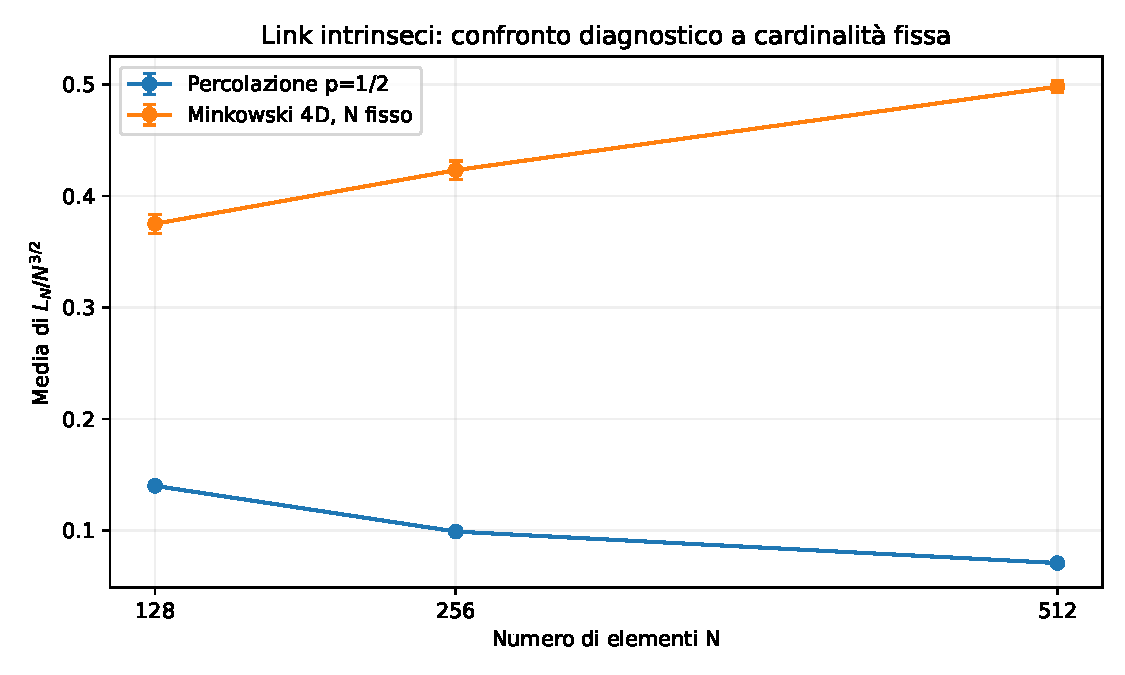
\includegraphics[width=0.91\linewidth]{R12BB_PI_LINK_SCALING.pdf}
\caption{Diagnostica \emph{finita}: media $L_N/N^{3/2}$ e barre di errore standard della media su 24 repliche. Non si adatta un esponente asintotico e non si inferisce una dinamica gravitazionale.}\end{figure}

\clearpage
\subsection*{Validazione, controllo delle esclusioni e decisione}
\textbf{Validazione matematica.} Due metodi indipendenti hanno analizzato tutte le $33\,867$ configurazioni di archi primitivi per $N=1,\ldots,6$ e tutti i $144$ campioni numerici. Il primo ricostruisce gli antenati e seleziona le coperture scorrendo i predecessori in ordine decrescente; il secondo ricostruisce i discendenti e trova gli elementi massimali sottraendo l'unione dei loro passati. I risultati esatti e i registri sono concordanti in tutti i casi. I valori medi esatti di $L_N$ per $N=2,3,4,5,6$ sono, rispettivamente, $1/2$, $11/8$, $161/64$, $3927/1024$, $172665/32768$; tutti soddisfano (PI.2).

\textbf{Casi non applicabili, senza modifiche a posteriori.} La condizione $|J(x)|\ge N/2$ fallisce per tutti gli $x$ in 14, 14 e 4 campioni Minkowski 4D alle tre taglie. Tali casi rimangono \texttt{NOT\_APPLICABLE} per $M_N$, non vengono trasformati in zeri, eliminati dal confronto globale dei link o usati per modificare il cutoff. La frazione ordinata $\overline r$ e coerente con la calibrazione 4D $r_4=1/10$ \emph{nelle taglie studiate}. Le medie Minkowski non provano una legge di scala universale a partire da tre dimensioni finite.

\textbf{Provenienza.} La disuguaglianza e l'idea di usare Borel--Cantelli sono nate in esplorazione \emph{prima} del congelamento; il protocollo numerico (SHA-256 integrale nel recovery; prefisso \texttt{b253adcaf41a777a}) e stato congelato \emph{prima} dell'esecuzione dei due programmi. Il generatore dei campioni e condiviso come stimolo testuale; le routine di transitive closure e di conteggio dei link sono indipendenti. Le prove all'infinito sono analitiche, non estrapolazioni dei $144$ campioni.

\textbf{Stato R12bb-PI:} \texttt{COVARIANT\_PRINCIPAL\_IDEAL\_LINK\_SCALING\_NULL\_MATH\_PASS}. Non sono selezionati la misura fisica, l'azione BDG nella misura, i vincoli QBC operatoriali noncommutativi, una geometria dinamica 4D o la legge autonoma $H(z)$. \textbf{R12bc NON APERTO; R12as fisico NON AUTORIZZATO; R13 BLOCCATO.}
Tutti i risultati precedenti, compresi i fallimenti, restano intatti.


\clearpage
\section*{Appendice v0.76 --- R12bb-SP: barriera di supporto per deformazioni sommabili}
\textbf{Domanda fisica e ambito del teorema.} Dopo gli audit v0.65 (accoppiamento modificato), v0.66 (due canali) e v0.73--v0.75 (eventi geometrici nulli), verifichiamo se deformazioni dei coefficienti di crescita possano modificare gli insiemi di storie a misura nulla. Il risultato riguarda una \emph{famiglia matematica} di crescita sequenziale complessa, non una nuova misura gravitazionale selezionata. Fissiamo senza cambiamenti $t_0=1$, $t_1=i$ e assumiamo
\begin{equation}
\boxed{\quad t_k=1+\delta_k>0\ \ (k\ge2),\qquad
D=\sum_{k=2}^{\infty}|\delta_k|<\infty,\quad \delta_k\in\mathbb R.\quad}
\tag{SP.1}
\end{equation}
La famiglia comprende il benchmark storico $\delta_k=0$ e la variante v0.65 $\delta_7=1$, tutte le altre $\delta_k=0$; \emph{non} include accoppiamenti arbitrari, singolari od operatoriali non commutanti.

Per un precursore $A$ che sia un \emph{downset} di un poset $C_n$, poniamo $w=|A|$ e $m=|\max A|$, con $w=m=0$ se $A=\varnothing$. Le normali formule della crescita sequenziale danno
\begin{align}
\lambda(w,m)&=\sum_{k=m}^{w}\binom{w-m}{k-m}t_k
=2^{w-m}+(i-1){\bf1}_{\{m=1\}}+\sum_{k=2}^{w}\delta_k\binom{w-m}{k-m},\tag{SP.2}\\
\Lambda_n&=\sum_{k=0}^{n}\binom nk t_k
=2^n+(i-1)n+\sum_{k=2}^{n}\delta_k\binom nk.\tag{SP.3}
\end{align}
Adott $C_n$, ogni downset $A$ puo essere prodotto scegliendo come archi primitivi diretti al nuovo elemento uno qualunque dei $2^{w-m}$ sottoinsiemi di $A$ contenenti tutti i massimali. Nella percolazione transitiva $P=P_{1/2}$,
\begin{equation}
P(A\mid C_n)=2^{-n}2^{w-m}.\tag{SP.4}
\end{equation}
Per ogni $k$ e ogni poset padre vale \emph{esattamente}
\begin{equation}
\boxed{\ \sum_{A\,\mathrm{downset}}\binom{|A|-|\max A|}{k-|\max A|}=\binom nk.\ }
\tag{SP.5}
\end{equation}
La prova e un conteggio doppio dei $k$-sottoinsiemi primitivi: il loro passato generato e un unico $A$, e per generarlo bisogna scegliere tutti i massimali di $A$. Ne segue $\sum_A\lambda(w,m)=\Lambda_n$, quindi la consistenza cilindrica.

\clearpage
\subsection*{Dimostrazione analitica: martingala e densita non nulla}
Definiamo il rapporto di ampiezza rispetto alla probabilita di transizione storica,
\begin{align}
q_n(A)&=\frac{\lambda(w,m)}{2^{w-m}},\qquad
c_n=\frac{2^n}{\Lambda_n},\qquad R_n(A)=c_nq_n(A),\tag{SP.6}\\
Z_N&=\prod_{n=0}^{N-1}R_n(A_n)=\frac{d\nu_N}{dP_N}.\tag{SP.7}
\end{align}
Grazie a (SP.5), $\mathbb E_P[R_n\mid\mathcal F_n]=1$: $Z_N$ e una martingala complessa normalizzata. Introduciamo la successione deterministica
\begin{equation}
e_n=2^{-n}\left(\sqrt2\,n+\sum_{k=2}^{n}|\delta_k|\binom nk\right),
\qquad M=\sqrt2+D.\tag{SP.8}
\end{equation}
Le identita di conteggio della precedente pagina danno, \emph{uniformemente sul poset padre},
\begin{equation}
\mathbb E_P[|q_n-1|\mid\mathcal F_n]\le e_n,\quad
|q_n-1|\le M,\quad
\mathbb E_P[|q_n|^2\mid\mathcal F_n]\le1+(2+M)e_n.\tag{SP.9}
\end{equation}
La serie binomiale $\sum_{n=k}^{\infty}\binom nk2^{-n}=2$ mostra che
\begin{equation}
\boxed{\ \sum_{n=0}^{\infty}e_n\le2\sqrt2+2D<\infty,\qquad
\sum_{n=0}^{\infty}\left|\frac{\Lambda_n-2^n}{2^n}\right|\le2\sqrt2+2D.\ }
\tag{SP.10}
\end{equation}
Ogni $\Lambda_n$ e non nullo: per $n\ge1$ ha parte immaginaria $n$, mentre $\Lambda_0=1$. Il prodotto $\prod_nc_n$ converge percio a un numero complesso finito e non nullo. Da (SP.9)--(SP.10) segue la stima \emph{uniforme in $N$}
\begin{equation}
\boxed{\ \sup_N\mathbb E_P|Z_N|^2\le
\left(\prod_{n=0}^{\infty}|c_n|^2\right)
\exp\left[(2+M)\sum_{n=0}^{\infty}e_n\right]
=:C_{\boldsymbol\delta}^2<\infty.\ }
\tag{SP.11}
\end{equation}
La martingala converge quindi in $L^2(P)$ e quasi sicuramente a $Z_\infty$ con $\mathbb E_PZ_\infty=1$. Inoltre $\sum_n|q_n-1|<\infty$ quasi sicuramente (Tonelli) e ogni $q_n\ne0$: $m=0$ da $1$, $m\ge2$ da $t_k>0$, $m=1$ dalla componente immaginaria $i$. Il prodotto $\prod_nq_n$ e dunque \emph{non nullo} quasi sicuramente. Percio $Z_\infty\ne0$ quasi sicuramente.

\clearpage
\subsection*{Teorema di invarianza dei nulli e vincolo quantitativo}
La misura complessa su eventi Borel infiniti e ora rappresentata da
\begin{equation}
\nu_{\boldsymbol\delta}(E)=\int_EZ_\infty\,dP,\qquad
|\nu_{\boldsymbol\delta}|(E)=\int_E|Z_\infty|\,dP.\tag{SP.12}
\end{equation}
Poiche $Z_\infty\ne0$ $P$-quasi sicuramente, la \emph{variazione totale positiva} e $P$ sono mutuamente assolutamente continue. Cosi,
\begin{equation}
\boxed{P(E)=0\ \Longleftrightarrow\ |\nu_{\boldsymbol\delta}|(E)=0;
\quad P(E)=0\ \Longrightarrow\ \mu_{\boldsymbol\delta}(E)=|\nu_{\boldsymbol\delta}(E)|^2=0.}
\tag{SP.13}
\end{equation}
Il verso inverso per $\mu$ non e assunto: interferenze possono annullare un'ampiezza anche per $P(E)>0$. Dagli audit precedenti segue per \emph{tutti} gli accoppiamenti (SP.1):
\begin{equation}
\boxed{\mu_{\boldsymbol\delta}(F_\varepsilon)=0\ (\varepsilon>0),\qquad
\nu_{\boldsymbol\delta}(E_{\mathrm{all}})=1,\ \mu_{\boldsymbol\delta}(E_{\mathrm{all}})=1.}
\tag{SP.14}
\end{equation}
Qui $F_\varepsilon$ richiede passati principali arbitrariamente grandi con almeno $\varepsilon |J|^{3/2}$ link (v0.75), mentre $E_{\mathrm{all}}$ richiede infiniti intervalli di ogni tipo finito (v0.74). La natura degli insiemi nulli resta quindi invariata \emph{anche se} i pesi di alcuni eventi non nulli cambiano sensibilmente.

Per Cauchy--Schwarz, $|\nu_{\boldsymbol\delta}(E)|\le C_{\boldsymbol\delta}\sqrt{P(E)}$ e
\begin{equation}
\boxed{\mu_{\boldsymbol\delta}(E)\le C_{\boldsymbol\delta}^2P(E).}
\tag{SP.15}
\end{equation}
Applicando il limite di Markov v0.75 all'evento \emph{etichettato} $B_N(\varepsilon)=\{L_N\ge\varepsilon N^{3/2}\}$,
\begin{equation}
\mu_{\boldsymbol\delta}(B_N(\varepsilon))\le
\frac{2C_{\boldsymbol\delta}^2}{\varepsilon\sqrt N}.\tag{SP.16}
\end{equation}
Questo \emph{cutoff di nascita} non e un evento covariante infinito. Piu in generale, per una densita di ampiezza vettoriale $h_N$ in uno spazio di Hilbert e un funzionale fortemente positivo $D_N(E,F)=\langle\Psi_N(E),\Psi_N(F)\rangle$, con $\Psi_N(E)=\int_Eh_N\,dP$, vale $\mu_N(E)\le\|h_N\|_2^2P(E)$, indipendentemente dal rango. Pertanto, se si volesse $\mu_N(B_N(\varepsilon))\ge\eta>0$, sarebbe \emph{necessario} che
\begin{equation}
\boxed{\|h_N\|_2\ge\sqrt\eta\,\sqrt{\varepsilon/2}\,N^{1/4}.}
\tag{SP.17}
\end{equation}
La divergenza richiesta non e una procedura sufficiente per ottenere gravita 4D: indica soltanto la necessaria uscita dalla classe $L^2$ uniformemente controllata (o dalla stessa misura di riferimento). Il caso a due canali commutativi v0.66 non elude (SP.13) quando ciascun canale appartiene alla famiglia.

\clearpage
\subsection*{Verifica indipendente, testimone storico e limiti fisici}
\textbf{Identita esatte su tutti i genitori finiti.} Il protocollo \texttt{R12BB\_SP\_PROTOCOL\_V076.json} e stato congelato \emph{dopo} l'esplorazione analitica e \emph{prima} dell'audit computazionale. Metodo A: costruzione dei poset per aggiunta di downset, codifica bitset; metodo B: enumerazione dei grafi primitivi, chiusura transitiva autonoma e raggruppamento degli insiemi di generatori. Entrambi verificano (SP.5) per ogni $k=0,\ldots,n$ e ogni genitore $n=0,\ldots,6$.

\begin{center}\small
\begin{tabular}{r|r|r}
$n$ & Genitori naturali & Configurazioni primitive\, ($n\ge1$)\\\hline
0 & 1 & --\\
1 & 1 & 1\\
2 & 2 & 2\\
3 & 7 & 8\\
4 & 40 & 64\\
5 & 357 & 1024\\
6 & 4824 & 32768\\\hline
Totale & 5232 & 33867
\end{tabular}
\end{center}
Il numero complessivo dei downset esaminati e $101\,659$ per metodo. Gli hash delle tabelle canoniche coincidono. Una prima asserzione dello script indipendente contava erroneamente $33\,867$ anche includendo il grafo vuoto $n=0$; l'asserzione e stata corretta a $33\,868$ \emph{con} il caso vuoto, senza filtrare risultati o modificare il teorema. Tale modifica e registrata nell'audit.

\textbf{Testimone fisso della v0.65.} Con un padre anticatena di sette elementi e il nuovo elemento sopra tutti, la variante $t_7=2$ ha peso $2$ anziche $1$, mentre $\Lambda_7$ passa da $121+7i$ a $122+7i$. Due algoritmi indipendenti confermano il rapporto delle misure dei cilindri
\begin{equation}
\boxed{\frac{\mu_{t_7=2}}{\mu_{t_7=1}}=
4\frac{121^2+7^2}{122^2+7^2}=
\frac{58760}{14933}.}\tag{SP.18}
\end{equation}
La differenza finita e reale, ma non modifica gli eventi $P$-nulli. Non e stato scelto un nuovo valore dopo aver osservato i risultati; e lo stesso confronto storico.

\textbf{Fonti e limiti.} La crescita sequenziale e i coefficienti $t_k$ sono descritti nella rassegna di Surya, \href{https://doi.org/10.1007/s41114-019-0023-1}{Living Reviews in Relativity (2019)}. L'importanza dell'estensione delle misure vettoriali e discussa da Dowker--Johnston--Surya, \href{https://arxiv.org/abs/1007.2725}{arXiv:1007.2725}. La classificazione QBC non commutativa resta distinta, cfr. Srivastava--Surya, \href{https://doi.org/10.1103/thx5-dknv}{Phys.~Rev.~D 114, 086007 (2026)}.

\textbf{Decisione scientifica R12bb-SP:} teorema di invarianza del supporto nullo nella famiglia (SP.1), verificato finitamente ma \emph{dimostrato} analiticamente; nessuna misura gravitazionale selezionata, nessuna azione BDG dinamica incorporata, QBC operatoriale noncommutativa o legge cosmologica $H(z)$ derivata. L'evento $F_\varepsilon$ non e stato dimostrato condizione necessaria di \emph{ogni} geometria 4D. \textbf{R12bc NON APERTO; R12as fisico NON AUTORIZZATO; R13 BLOCCATO.}


\clearpage
\section*{Appendice v0.77 --- R12bb-RT: rarita quantitativa dei link e barriera per le ampiezze}
\textbf{Obiettivo.} La v0.75 ha mostrato, per la percolazione transitiva storica $P_{1/2}$, che $L_N/N^{3/2}\to0$ quasi sicuramente; la v0.76 ha esteso gli insiemi nulli a un'intera famiglia di misure complesse, ricavando dal limite di Markov solo un ostacolo quantitativo di ordine $N^{-1/2}$. Senza modificare $p=1/2$ o alcun coefficiente storico, rafforziamo il \emph{limite sulle probabilita finite}. La prova e elementare, e non seleziona una misura gravitazionale.

\textbf{Modello.} Gli archi primitivi $i\to j$ ($0\le i<j<N$) sono indipendenti, ciascuno presente con probabilita $1/2$; la chiusura transitiva definisce il poset. $L_N$ conta le sue \emph{coperture} (link). Per $\varepsilon>0$ e $N\ge2$ fissiamo
\begin{equation}
 B_N(\varepsilon)=\{L_N\ge\varepsilon N^{3/2}\},\qquad
 K_N(\varepsilon)=\lceil\varepsilon\sqrt{N}\rceil-1.\tag{RT.1}
\end{equation}
L'evento $B_N$ e una proprieta intrinseca del poset \emph{finito} dopo $N$ nascite; il suo particolare cutoff non e, da solo, un evento covariante sulla totalita delle storie infinite.

\textbf{Lemma del link lungo.} Per una coppia $i<j$, $d=j-i$, essere un link richiede la presenza dell'arco diretto $i\to j$ e l'assenza di ogni percorso primitivo a due passi $i\to k\to j$ con $i<k<j$. Questi $d-1$ possibili percorsi a due passi dipendono da coppie disgiunte di variabili di arco, e ciascuno compare con probabilita $1/4$. Ne segue il limite esatto sulle condizioni necessarie
\begin{equation}
 \boxed{\ P_{1/2}\bigl((i,j)\ \mathrm{link}\bigr)
 \le\frac12\left(\frac34\right)^{j-i-1}.\ }\tag{RT.2}
\end{equation}
Non si assume indipendenza fra gli \emph{indicatori} dei link. Se tutti i link avessero distanza di nascita $j-i\le K$, ce ne sarebbero al massimo $NK$. Poiche $K_N(\varepsilon)<\varepsilon\sqrt N$, ogni configurazione in $B_N(\varepsilon)$ deve contenere almeno un link con $j-i\ge K_N+1$. Applicando solo l'union bound otteniamo, \emph{per ogni} $N\ge2$,
\begin{equation}
 \boxed{\ P_{1/2}\bigl(B_N(\varepsilon)\bigr)
 \le \min\left\{1,\ 2N\left(\frac34\right)^{K_N(\varepsilon)}\right\}.\ }\tag{RT.3}
\end{equation}
L'evento e vuoto se $\varepsilon N^{3/2}>\binom N2$. Il limite e al piu $O\!\left(N e^{-\varepsilon\log(4/3)\sqrt N}\right)$; \emph{non} e stata dimostrata una formula asintotica esatta per la probabilita. Il precedente Markov forniva solo $P(B_N)<2/(\varepsilon\sqrt N)$.

\clearpage
\subsection*{Certificati razionali, confronto dei limiti e limiti a piccoli tagli}
Per il valore diagnostico razionale $\varepsilon=1/4$ (non selezionato da fit cosmologici), $K_N=\lceil\sqrt N/4\rceil-1$ si calcola usando esclusivamente radici quadrate intere; l'espressione $2N\cdot 3^{K_N}/4^{K_N}$ e una frazione \emph{esatta}. La figura riporta soltanto gli \emph{upper bound}, non frequenze empiriche ne probabilita effettive.
\begin{center}\small
\begin{tabular}{r r r r}
\toprule
$N$ & $K_N$ & RT.3 (massimo) & Markov (massimo)\\
\midrule
$10^4$ & 24 & $1$ (non informativo) & $8,00\cdot10^{-2}$\\
$10^5$ & 79 & $2,70\cdot10^{-5}$ & $2,53\cdot10^{-2}$\\
$10^6$ & 249 & $1,55\cdot10^{-25}$ & $8,00\cdot10^{-3}$\\
$10^7$ & 790 & $3,98\cdot10^{-92}$ & $2,53\cdot10^{-3}$\\
\bottomrule
\end{tabular}
\end{center}
\begin{figure}[H]\centering
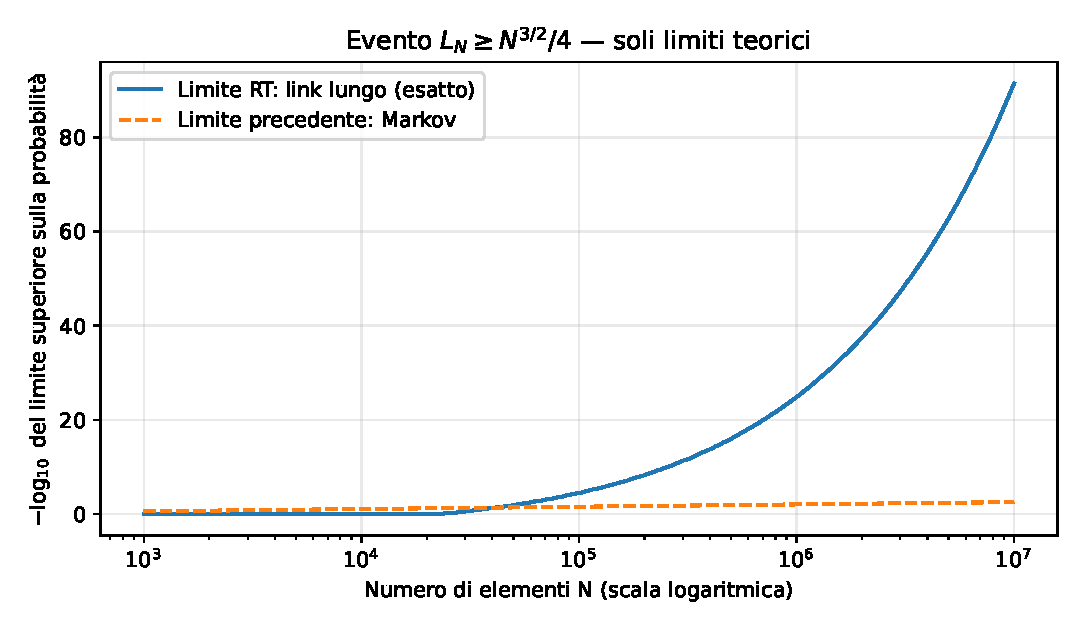
\includegraphics[width=0.90\linewidth]{R12BB_RT_RARITY_BOUND.pdf}
\caption{Limiti superiori certificati per $B_N(1/4)$. L'asse verticale rappresenta $-\log_{10}$ del \emph{limite superiore}: un valore maggiore significa soltanto una stima piu restrittiva. Nessuna curva rappresenta una simulazione.}
\end{figure}
I valori numerici sono visualizzazioni di frazioni razionali certificate; eventuali approssimazioni floating point non entrano nella prova. Ai tagli piccoli RT.3 puo essere uguale a 1: l'assenza di potere diagnostico e registrata, senza modificare $\varepsilon$.

\clearpage
\subsection*{Vincolo necessario sulle misure quantistiche vettoriali}
Sullo spazio degli esiti finiti sia $h_N$ una densita a valori in uno spazio di Hilbert complesso $\mathcal H$ rispetto a $P_{1/2,N}$. Definiamo una misura vettoriale $\Psi_N(E)=\int_Eh_N\,dP_{1/2,N}$ e la sua misura quantistica fortemente positiva $\mu_N(E)=\|\Psi_N(E)\|_{\mathcal H}^2$. Per Cauchy--Schwarz vale
\begin{equation}
\mu_N(B_N)\le\|h_N\|_{L^2(P;\mathcal H)}^2\,P_{1/2}(B_N).\tag{RT.4}
\end{equation}
Se si richiede $\mu_N(B_N(\varepsilon))\ge\eta>0$, la disuguaglianza RT.3 impone la \emph{condizione necessaria}
\begin{equation}
\boxed{\ \|h_N\|_{2}\ge\sqrt{\frac{\eta}{2N}}
\left(\frac43\right)^{K_N(\varepsilon)/2}.\ }\tag{RT.5}
\end{equation}
Per $\varepsilon,\eta$ fissi e tagli $N$ arbitrariamente grandi, la crescita richiesta e almeno \emph{stretched-exponential} in $\sqrt N$. La dimensione di $\mathcal H$ non compare nella prova: il limite vale anche per misure vettoriali di rango arbitrario e non presuppone che gli operatori di crescita commutino. Non dimostra, tuttavia, \emph{l'esistenza} di una crescita noncommutativa QBC coerente.

Piu in generale, per $q>1$ la disuguaglianza di H\"older da
\begin{equation}
 \mu_N(B_N)\le\|h_N\|_q^2P_{1/2}(B_N)^{2(1-1/q)};
 \quad \mu_N(B_N)\ge\eta\ \Longrightarrow\ 
 \|h_N\|_q\ge\sqrt\eta\,(2N)^{-(1-1/q)}
 \left(\frac43\right)^{K_N(1-1/q)}.\tag{RT.6}
\end{equation}
\textbf{Confronto, non identificazione:} per una \emph{distribuzione classica positiva} $Q_N$ con $Q_N(B_N)\ge\eta$, la disuguaglianza informazionale standard da $D_{\mathrm{KL}}(Q_N\|P_N)\ge\eta\log[1/P_N(B_N)]-\log2$, quindi un costo almeno di ordine $\sqrt N$ se $\eta$ rimane costante. Non applicare questa entropia classica a un'ampiezza complessa.

\clearpage
\subsection*{Versione intrinseca finita, audit indipendente e limiti}
Uno \emph{stem principale} $J(x)=\{y:y\preceq x\}$ e un downset. Su un poset finito di $N$ elementi consideriamo
\begin{equation}
 C_N(\varepsilon)=\{\exists x:\ |J(x)|\ge N/2,\;
 L(J(x))\ge\varepsilon |J(x)|^{3/2}\}.\tag{RT.7}
\end{equation}
Questa proprieta e intrinseca al \emph{poset finito}. Poiche ogni cover di $J(x)$ rimane tale nell'intero poset, $L_N\ge L(J(x))$ e
\begin{equation}
 \boxed{C_N(\varepsilon)\subseteq B_N\left(\frac{\varepsilon}{2\sqrt2}\right).}\tag{RT.8}
\end{equation}
RT.3 fornisce dunque un limite stretched-exponential anche per RT.7. Attenzione: \emph{l'esistenza di uno stem con tale proprieta in una storia infinita} e un evento diverso, che puo comportarsi diversamente (v0.74); non lo identifichiamo con un prefisso selezionato da un ordine di nascita.

\textbf{Audit esatto.} Protocollo congelato prima della validazione: 
\texttt{R12BB\_RT\_PROTOCOL\_V077.json}, SHA-256 nel recovery. Due programmi separati ricostruiscono tutte le $33\,868$ configurazioni primitive di dimensioni $N=0,\ldots,6$ usando rispettivamente bitset in ordine discendente e chiusura booleana Floyd--Warshall. Per i due valori diagnostici $\varepsilon=1/4,1/2$ concordano \emph{byte per byte} su istogrammi di $L_N$, conteggi dei link per distanza, condizioni B e C, disuguaglianza RT.2 per ogni coppia e testimone deterministico del link lungo. La tabella delle soglie grandi e certificata con frazioni razionali: non e un esperimento Monte Carlo.

\textbf{QA e validita.} La ricerca della disuguaglianza precede il congelamento del protocollo. In debug sono stati corretti tre errori meramente software: il caso vacuo $N=0$ (da escludere da $B_N$), il parsing di una chiave di coppia e la chiamata accidentale di una lista come funzione; nessun campione o risultato sfavorevole e stato scartato. Il limite RT.3 e dimostrato per il benchmark $p=1/2$; la sua forma elementare non e rivendicata come nuova rispetto a tutta la letteratura sui \emph{random graph orders} (Rideout--Sorkin, \href{https://doi.org/10.1103/PhysRevD.61.024002}{PRD 61, 024002}; Surya, \href{https://doi.org/10.1007/s41114-019-0023-1}{Living Reviews 2019}). Non segue una misura fisica selezionata, la dinamica BDG, i vincoli QBC noncommutativi, la gravita 4D o una previsione $H(z)$.

\textbf{Decisione R12bb-RT:} \texttt{RT\_MATH\_PASS}; \textbf{R12bc NON APERTO; R12as fisico NON AUTORIZZATO; R13 BLOCCATO.}
Tutti i risultati storici positivi, negativi o inconcludenti restano preservati.

\clearpage
\section*{R12bb-BD --- Degenerazione esatta dell'azione BDG in dimensione quattro (v0.78)}
\textbf{Domanda e dominio.} Le versioni v0.73--v0.77 hanno stabilito criteri geometrici che il benchmark di percolazione e un'ampia classe di misure complesse non riescono a sostenere. Esaminiamo ora un ingrediente fisico gia presente nella ricerca: \emph{il valore dell'azione discreta Benincasa--Dowker--Glaser (BDG) 4D}, senza introdurre nuovi coefficienti o una nuova misura. La domanda e se tale valore, preso da solo, separi strutture causali macroscopicamente differenti.

Per un causal set finito $C$ di $N$ elementi, definiamo $N_k(C)$ come il numero di coppie comparabili $(x,y)$ con esattamente $k$ elementi \emph{strettamente} nell'intervallo causale $(x,y)$. L'indice combinatorio BDG storico e
\begin{equation}
 Q_4(C)=N-N_0(C)+9N_1(C)-16N_2(C)+8N_3(C),\qquad
 \frac{S_{\rm BDG}(C)}{\hbar}=\theta Q_4(C),\quad\theta=\frac4{\sqrt6}.
 \tag{BD.1}
\end{equation}
Si mantiene il valore diagnostico gia fissato $\ell/\ell_P=1$, senza termini di bordo aggiuntivi o smearing della formula. La stessa forma degli osservabili per intervalli e standard nella letteratura BDG (Benincasa--Dowker 2010; Adamson--Wallden, \href{https://doi.org/10.1103/qdst-yrh6}{Phys. Rev. Research 8, 023188, 2026}). La dimostrazione che segue e un'identita combinatoria limitata a BD.1, non un teorema sul path sum fisico.

\subsection*{BD.1 --- Famiglia esattamente degenere a ogni cardinalita}
Sia $K_c$ una catena totale di $c$ elementi, $A_{N-c}$ un'anticatena isolata dal resto, e $C_{N,c}=K_c\sqcup A_{N-c}$, con $4\le c\le N$. Le uniche relazioni comparabili sono nella catena. Per $k=0,1,2,3$,
\begin{equation}
 N_k(C_{N,c})=c-k-1\qquad(c\ge4),
 \tag{BD.2}
\end{equation}
intendendo $N_3=0$ quando $c=4$. Di conseguenza,
\begin{align}
 Q_4(C_{N,c})&=N-(c-1)+9(c-2)-16(c-3)+8(c-4)\notag\\
 &=\boxed{N-1}.\tag{BD.3}
\end{align}
Anche un ordine formato da una singola relazione e da $N-2$ elementi isolati ha $N_0=1$, $N_{1,2,3}=0$, quindi \emph{esattamente lo stesso indice} $Q_4=N-1$. Nella somma Lorentziana pesata solo dalla fase BDG, ciascuna delle storie qui considerate porta il fattore $\exp[i\theta(N-1)]$.

Questo identifica una vera degenerazione dell'\emph{osservabile azione}. Non dichiara uguali i coefficienti di misura dei diversi causal set, ne il numero delle loro etichettature naturali, ne le ampiezze complessive del path sum; la misura fisica rimane non derivata.

\subsection*{BD.2 --- La stessa azione non fissa neppure l'ordine di comparabilita}
Per $C_{N,c}$, la frazione di coppie causalmente ordinate e l'altezza massima valgono
\begin{equation}
 r(C_{N,c})=\frac{c(c-1)}{N(N-1)},\qquad H(C_{N,c})=c.
 \tag{BD.4}
\end{equation}
Fissato qualunque $\rho\in[0,1]$, scegliendo
\begin{equation}
 c_N=\max\{4,\min[N,\lfloor\sqrt\rho\,N\rfloor]\}
 \quad(N\ge4),\qquad
 \lim_{N\to\infty}r(C_{N,c_N})=\rho,\quad Q_4(C_{N,c_N})=N-1,
 \tag{BD.5}
\end{equation}
si ottiene una famiglia che realizza ogni frazione d'ordine limite, pur mantenendo l'identico valore dell'indice BDG a parita di $N$. Il valore $\rho=1/10$ ricorda la diagnostica cinematica della v0.69, \emph{ma non rende queste catene con isolati simili a uno spazio-tempo di Minkowski 4D}: altezza, intervalli e altre diagnostiche differiscono nettamente.

\begin{center}\small
\begin{tabular}{lrrrrrrr}
\toprule
Causal set con $N=6$ & $R$ & $H$ & $N_0$ & $N_1$ & $N_2$ & $N_3$ & $Q_4$\\
\midrule
Un solo legame; altri isolati & 1 & 2 & 1 & 0 & 0 & 0 & 5\\
Catena di 4; due isolati & 6 & 4 & 3 & 2 & 1 & 0 & 5\\
Catena completa di 6 & 15 & 6 & 5 & 4 & 3 & 2 & 5\\
\bottomrule
\end{tabular}
\captionof{table}{Tre strutture causalmente distinte con indice BDG esattamente identico. $R$ e il numero di coppie ordinate; $H$ e l'altezza (catena massima).}
\end{center}

\subsection*{BD.3 --- Censimento esatto e validazione indipendente}
Il protocollo \texttt{R12BB\_BD\_PROTOCOL\_V078.json}, SHA-256 \texttt{90ea85a9c2287e79b1cca265d369b01d}\linebreak\texttt{f6567d50d1ee2c52f6c6d4e524170133}, e stato congelato \emph{dopo} la scoperta esplorativa dell'identita BD.3 e \emph{prima} della validazione indipendente dei codici. Non si rivendica una scoperta preregistrata.

Il primo programma enumera tutti i $2^{\binom N2}$ grafi primitivi per $N=0,\dots,6$, ne calcola la chiusura transitiva mediante bitset e deduplica i poset naturalmente etichettati. Il secondo costruisce invece direttamente, mediante aggiunta successiva di un massimo con passato downset, tutti i poset naturalmente etichettati; determina intervalli e altezza con un procedimento separato. I due risultati JSON coincidono \emph{byte per byte}, compresi tutti gli istogrammi di $Q_4$:
\begin{equation}
 \#\mathcal P^{\rm natural}_{N=0,\ldots,6}=1+1+2+7+40+357+4824=5232.
 \tag{BD.6}
\end{equation}
Sono stati controllati anche $33\,868$ grafi primitivi (incluso $N=0$). Per $N=6$ esistono 54 valori distinti di $Q_4$ e 53 poset \emph{naturalmente etichettati} con $Q_4=5$; fra questi $R$ varia da 1 a 15 e $H$ da 2 a 6. Sono conteggi dell'insieme naturalmente etichettato, \textbf{non} conteggi di classi di isomorfismo e \textbf{non} degenerazioni di una misura gravitazionale non etichettata. Il codice verifica inoltre BD.3 per le famiglie prescritte a $4\le N\le12$; la verita per tutti gli $N\ge4$ discende dalla prova algebrica, non da questi controlli finiti.

\textbf{Decisione e limiti.} L'azione BDG 4D, come \emph{un singolo numero} su un poset finito, non identifica una geometria ne una dimensione fisica: famiglie con diversa frazione ordinata e diversa altezza possono avere esattamente la stessa fase. Non segue che l'intero path sum con pesi, interferenze ed entropia sia incapace di selezionare geometrie 4D, ne che l'azione BDG sia fisicamente inutile. La dimostrazione non comprende termini di bordo/smearing, misure operatoriali QBC, risposta gravitazionale o un limite 4D selezionato. \textbf{R12bb-BD: identita e audit matematici PASS; R12bc NON APERTO; R12as fisico NON AUTORIZZATO; R13 BLOCCATO.} Non e stata derivata alcuna nuova legge autonoma $H(z)$.



\clearpage
\section*{R12bb-ES --- Molte classi non isomorfe con identica fase BDG (v0.79)}
\textbf{Domanda.} Il gate v0.78 ha mostrato che una singola catena con isolati puo mantenere l'indice gravitazionale BDG 4D identico a quello di un solo legame. Il nuovo controllo distingue una mera famiglia a un parametro da una \emph{molteplicita crescente di classi di isomorfismo} a cardinalita e fase fissate. Nessun coefficiente BDG o parametro fisico viene cambiato.

Per un poset finito $C$, manteniamo esattamente l'indice non smoothed gia congelato,
\begin{equation}
 Q_4(C)=|C|-N_0(C)+9N_1(C)-16N_2(C)+8N_3(C),
 \qquad S_{\rm BDG}(C)/\hbar=\theta Q_4(C),\quad \theta=4/\sqrt6.
 \tag{ES.1}
\end{equation}
Indichiamo con $K_j$ la catena di $j$ elementi e con $A_j$ un'anticatena di $j$ isolati. Per disgiunzioni senza comparabilita tra blocchi, tutti i conteggi $N_k$ e il termine $|C|$ sono additivi; perci\`o $Q_4$ e additivo. Le identita di base sono
\begin{equation}
 \begin{aligned}
 Q_4(K_2)&=1,&Q_4(K_3)&=10,& Q_4(K_c)&=c-1 \quad(c\ge4),\\
 Q_4(A_j)&=j.& & &
 \end{aligned}\tag{ES.2}
\end{equation}
La seconda riga di ES.2 per le anticatene non equivale a un contributo dinamico: non vi sono intervalli comparabili, quindi resta solo la cardinalita.

Per un intero $m\ge1$ poniamo $c_i=i+3$ ($i=1,\ldots,m$) e
\begin{equation}
 B_m=\sum_{i=1}^m(c_i+15)=\frac{m(m+37)}{2},\qquad
 N_m=2B_m=m(m+37).\tag{ES.3}
\end{equation}
Definiamo due scelte per un \emph{blocco neutro} di $c_i+15$ elementi:
\begin{equation}
 G_i^{(0)}=A_{c_i+15},\qquad
 G_i^{(1)}=K_{c_i}\sqcup K_3\sqcup\Bigl(\bigsqcup_{j=1}^{6}K_2\Bigr).
 \tag{ES.4}
\end{equation}
Entrambe hanno la stessa cardinalita e \emph{esattamente} lo stesso indice:
\begin{equation}
 Q_4(G_i^{(0)})=c_i+15,
 \quad Q_4(G_i^{(1)})=(c_i-1)+10+6=c_i+15.
 \tag{ES.5}
\end{equation}
La parte macroscopica ha due scelte di $B_m$ elementi:
\begin{equation}
 M^{(0)}=K_2\sqcup A_{B_m-2},\qquad M^{(1)}=K_{B_m},\qquad
 Q_4(M^{(0)})=Q_4(M^{(1)})=B_m-1.
 \tag{ES.6}
\end{equation}
Ogni vettore binario $\sigma=(\sigma_0,\ldots,\sigma_m)$ definisce
\begin{equation}
 \boxed{\ C_{m,\sigma}=M^{(\sigma_0)}\sqcup\biggl(\bigsqcup_{i=1}^m G_i^{(\sigma_i)}\biggr),
 \qquad |C_{m,\sigma}|=N_m,\quad Q_4(C_{m,\sigma})=N_m-1.\ }
 \tag{ES.7}
\end{equation}
L'identita vale per \emph{tutti} i $2^{m+1}$ vettori; non deriva da un fitting o da un censimento finito.

\clearpage
\subsection*{ES.1 --- Non isomorfismo, osservabili geometrici e crescita della molteplicit\`a}
Tutti i $C_{m,\sigma}$ sono unioni disgiunte di catene. Il multinsieme delle lunghezze delle componenti connesse (considerando il grafo non orientato di comparabilita) \`e un \emph{invariante completo di isomorfismo} in questa sottoclasse. Le uniche componenti di lunghezza almeno quattro hanno lunghezza $c_i=i+3$ precisamente se $\sigma_i=1$ e lunghezza $B_m$ precisamente se $\sigma_0=1$. Poiche $B_m>m+3=c_m$, tutte le scelte sono identificabili dal solo poset non etichettato. Quindi:
\begin{equation}
 \boxed{\#\{[C_{m,\sigma}]:\sigma\in\{0,1\}^{m+1}\}=2^{m+1},
 \qquad Q_4=N_m-1,\quad N_m=m(m+37).}\tag{ES.8}
\end{equation}
Si tratta di un \emph{limite inferiore} sulla molteplicit\`a complessiva del livello di azione. In particolare $\log(\#)=(m+1)\log2=\Omega(\sqrt{N_m})$: l'insieme di classi esattamente a pari fase cresce almeno in modo stretched-exponential lungo la successione ES.3. Non viene dichiarato un limite asintotico per la frazione di tutte le geometrie possibili.

Indichiamo con $R(C)$ il numero di coppie comparabili, con $H(C)$ l'altezza e con $r(C)=2R/[N(N-1)]$ la frazione ordinata. Il numero di coppie e
\begin{equation}
 R(C_{m,\sigma})=
 \begin{cases}\binom{B_m}{2},&\sigma_0=1,\\1,&\sigma_0=0,\end{cases}
 +\sum_{i:\sigma_i=1}\left[\binom{c_i}{2}+9\right].\tag{ES.9}
\end{equation}
Il minimo assoluto corrisponde alla macro-scena con una sola relazione e ai blocchi neutri isolati ($R_{\min}=1$, $H=2$). Il massimo corrisponde a tutte le catene attive:
\begin{equation}
 R_{\max}=\binom{B_m}{2}+\sum_{i=1}^m\left[\binom{i+3}{2}+9\right],\qquad
 r_{\min}\longrightarrow0,\quad r_{\max}\longrightarrow\frac14.
 \tag{ES.10}
\end{equation}
Infatti $B_m=\Theta(m^2)$, mentre la somma delle relazioni nei gadget cresce solo come $O(m^3)$; il blocco macro genera un contributo $\Theta(m^4)$.

\begin{center}\small
\begin{tabular}{rrrrr}
\toprule
$m$ & $N_m$ & $Q_4$ & classi distinte certificate & $R_{\min}\ \ldots\ R_{\max}$\\
\midrule
1 & 38 & 37 & 4 & $1\ldots186$\\
2 & 78 & 77 & 8 & $1\ldots775$\\
3 & 120 & 119 & 16 & $1\ldots1828$\\
5 & 210 & 209 & 64 & $1\ldots5585$\\
7 & 308 & 307 & 256 & $1\ldots12005$\\
\bottomrule
\end{tabular}
\captionof{table}{Risultati esatti per una selezione prefissata di cardinalit\`a. Le classi sono non isomorfe, non semplici etichette di uno stesso ordine.}
\end{center}
\begin{figure}[H]\centering
 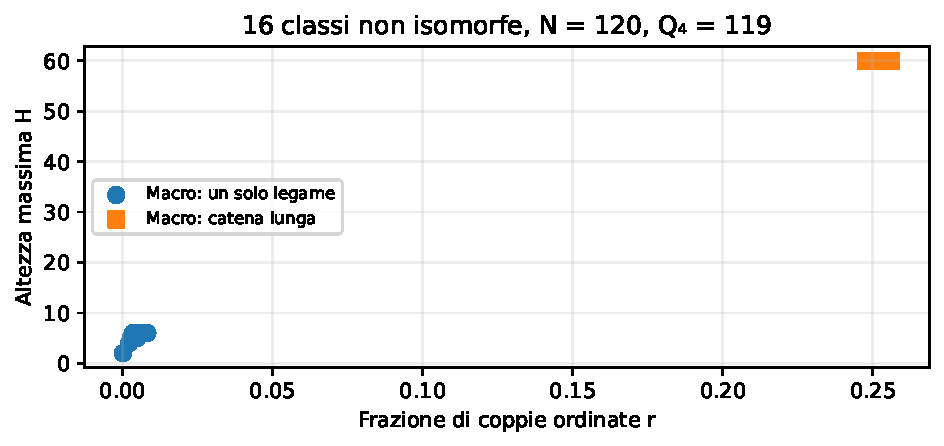
\includegraphics[width=0.80\linewidth]{R12BB_ES_DEGENERACY_SPECTRUM.pdf}
 \caption{Testimone a 120 elementi: 16 poset non isomorfi con $Q_4=119$, ma con altezza e frazione ordinata variabili. Il grafico \`e un controllo illustrativo della formula, non una simulazione cosmologica.}
\end{figure}

\clearpage
\subsection*{ES.2 --- Interferenza di fase, audit e limiti fisici}
Per la fase storica $\theta=4/\sqrt6$, ciascun elemento \emph{della sottoclasse esplicita} ha
\begin{equation}
 e^{i S_{\rm BDG}(C_{m,\sigma})/\hbar}=e^{i\theta(N_m-1)}.
 \tag{ES.11}
\end{equation}
\emph{Come sola identit\`a di bookkeeping} e senza pretendere che corrisponda alla misura gravitazionale fisica, la somma che attribuisce peso unitario a \emph{una classe per isomorfismo} d\`a
\begin{equation}
 Z_m^{\rm unit\`a}=\sum_{\sigma\in\{0,1\}^{m+1}}
 e^{i\theta Q_4(C_{m,\sigma})}=2^{m+1}e^{i\theta(N_m-1)}.
 \tag{ES.12}
\end{equation}
Nella sottoclasse non vi sono cancellazioni \emph{dovute alla sola fase BDG}; tale fatto non vieta cancellazioni con altri livelli d'azione o con fasi della misura. La misura fisica potrebbe dipendere da isomorfismi, automorfismi, fattori di normalizzazione, etichettature naturali, geometria, condizioni al bordo o dinamica quantistica noncommutativa. Sostituirla con pesi uniformi \`e un'illustrazione matematica, \textbf{non} una deduzione autorizzata.

\textbf{Validazione dopo la scoperta analitica.} Il protocollo \texttt{R12BB\_ES\_PROTOCOL\_V079.json} \`e stato congelato \emph{dopo} la costruzione ES.4--ES.8 e \emph{prima} dell'audit indipendente. Un codice genera gli ordini causali e calcola ogni intervallo con maschere di bit; un secondo codice lavora direttamente con la decomposizione in componenti e formule sui conteggi. I due JSON sono byte-identici. Sono state controllate tutte le $508$ scelte per $m=1,\ldots,7$, senza scarti, verificando $Q_4$, cardinalit\`a, $R$, $H$, i quattro $N_k$ e le firme di isomorfismo; sono presenti inoltre certificati analitici per $m=8,12,20,40,80$ (questi ultimi \emph{non} sono censimenti esaustivi). L'esattezza per $m$ arbitrario discende da ES.2--ES.8.

La relazione fra entropia dei causal set e soppressione tramite interferenza nei path sum \`e studiata, in termini differenti, da Loomis--Carlip (\href{https://doi.org/10.1088/1361-6382/aa980b}{Class. Quantum Grav. 35, 024002}) e da Mathur--Singh--Surya (\href{https://arxiv.org/abs/2009.07623}{arXiv:2009.07623}). Non rivendichiamo che il limite inferiore ES.8 stabilisca dominanza statistica, misura fisica, preferenza per geometrie non-variet\`a o mancanza di una fase semiclassica.

\textbf{Decisione R12bb-ES:} \texttt{FIXED\_ACTION\_CLASS\_MULTIPLICITY\_MATH\_PASS}. Questo risultato rafforza il fatto che la fase BDG scalare non pu\`o, da sola, distinguere i membri del livello costruito, ma \textbf{non} seleziona una misura quantistica 4D. R12bc resta \textbf{NON APERTO}; R12as fisico \textbf{NON AUTORIZZATO}; R13 \textbf{BLOCCATO}. Nessuna nuova legge autonoma $H(z)$ \`e stata ricavata.

\clearpage
\section*{R12bb-GW --- L'etichettatura naturale non seleziona la misura fisica (v0.80)}
\textbf{Domanda.} Nella v0.79 abbiamo costruito $2^{m+1}$ causal set non isomorfi con cardinalita $N=m(m+37)$ e indice BDG $Q_4=N-1$. La fase Lorentziana e identica. La domanda qui e se il \emph{numero di classi di isomorfismo} coincida con il numero di \emph{matrici di ordine naturalmente etichettate}. Non imponiamo che uno di questi conteggi sia una misura gravitazionale fisica. Non modifichiamo l'azione BDG, i parametri di fase o i risultati storici.

Un causal set non etichettato formato da una unione disgiunta di catene ha $n_\ell$ componenti di lunghezza $\ell$, e $N=\sum_{\ell\ge1}\ell n_\ell$ elementi. Il numero di \emph{estensioni lineari} di una rappresentazione con componenti temporaneamente distinguibili e
\begin{equation}
 e(C)=\frac{N!}{\prod_{\ell\ge1}(\ell!)^{n_\ell}}.
 \tag{GW.1}
\end{equation}
Gli automorfismi del poset sono esattamente le permutazioni delle catene di uguale lunghezza: $|\operatorname{Aut}(C)|=\prod_{\ell\ge1}n_\ell!$. Una stessa matrice naturalmente etichettata e contata $|\operatorname{Aut}(C)|$ volte fra le estensioni distinte su elementi astratti, quindi
\begin{equation}
 \boxed{W_{\rm nat}(C)=\frac{e(C)}{|\operatorname{Aut}(C)|}
 =\frac{N!}{\displaystyle\prod_{\ell\ge1}(\ell!)^{n_\ell}n_\ell!}.}
 \tag{GW.2}
\end{equation}
$W_{\rm nat}$ e un \emph{intero} e conta le distinte relazioni d'ordine sui nomi $1,\ldots,N$ che sono compatibili con l'ordine di nascita. E un conteggio, non una probabilita o una prescrizione di path integral; in una teoria generalmente covariante gli ordinamenti di nascita possono essere ridondanze descrittive e non stati fisici indipendenti.

Per la famiglia v0.79, scriviamo $B=N/2=m(m+37)/2$, $c_i=i+3$, $\sigma=(b_0,b_1,\ldots,b_m)$ e $t=\sum_{i=1}^m b_i$. I numeri di componenti di lunghezza uno, due e tre sono
\begin{equation}
 \begin{aligned}
 n_1&=(1-b_0)(B-2)+\sum_{i:b_i=0}(c_i+15),\\
 n_2&=(1-b_0)+6t,\qquad n_3=t,\\
 n_{c_i}&=b_i\ (c_i\ge4),\qquad n_B=b_0.
 \end{aligned}\tag{GW.3}
\end{equation}
Poiche $c_i\neq c_j$ per $i\neq j$ e $B>c_m$, queste componenti hanno lunghezze distinguibili; percio
\begin{equation}
 \boxed{W_m(\sigma)=\frac{N!}{n_1!\,2^{n_2}n_2!\,6^t t!\,
 (B!)^{b_0}\prod_{i:b_i=1}c_i!}.}
 \tag{GW.4}
\end{equation}
La fase $\exp[i(4/\sqrt6)(N-1)]$ resta identica per \emph{tutti} i $\sigma$; i pesi $W_m(\sigma)$ invece no.

\clearpage
\subsection*{GW.1 --- Controesempio quantitativo: due convenzioni, stessa azione}
Scegliamo due \emph{membri gia presenti} della famiglia v0.79, con $b_i=0$ per ogni $i\ge1$; cambiamo soltanto $b_0$:
\begin{equation}
 C_0=K_2\sqcup A_{N-2},\qquad C_1=K_B\sqcup A_B,
 \qquad N=2B,\quad Q_4(C_0)=Q_4(C_1)=N-1.\tag{GW.5}
\end{equation}
I conteggi su classi non etichettate attribuiscono \emph{una} classe a ciascuna delle due geometrie. Invece la molteplicit\`a delle relazioni naturalmente etichettate e
\begin{equation}
 W_{\rm nat}(C_0)=\binom N2,\quad
 W_{\rm nat}(C_1)=\binom N{N/2},\qquad
 \frac{W_{\rm nat}(C_1)}{W_{\rm nat}(C_0)}
 =\frac{\binom N{N/2}}{\binom N2}.
 \tag{GW.6}
\end{equation}
Poiche $\binom N{N/2}$ e il massimo coefficiente binomiale, e quindi almeno la media $2^N/(N+1)$, si ha \emph{per ogni $N$ della costruzione}
\begin{equation}
 \boxed{\frac{W_{\rm nat}(C_1)}{W_{\rm nat}(C_0)}
 \ge \frac{2^{N+1}}{N(N-1)(N+1)}.}
 \tag{GW.7}
\end{equation}
La disparita \`e almeno esponenziale in $N$ e non nasce dalla fase BDG. La convenzione alternativa di un fattore $1/|\operatorname{Aut}(C)|$ per ogni classe non etichettata produce invece
\begin{equation}
 \frac{1/|\operatorname{Aut}(C_1)|}{1/|\operatorname{Aut}(C_0)|}
 =\frac{(N-2)!}{B!},\tag{GW.8}
\end{equation}
ancora un rapporto diverso. I tre pesi \textbf{non sono intercambiabili}: classe unitaria, numero di etichette naturali e inverso del gruppo di automorfismi sono convenzioni diagnostiche distinte.

\begin{center}\small
\begin{tabular}{rrrrr}
\toprule
$m$ & $N$ & classi non isomorfe & $\log_{10}[W_1/W_0]$ & percentuale macro-$K_B$ nell'intera famiglia\\
\midrule
1&38&4&7.701&3.9326\\
2&78&8&18.957&1.7241\\
3&120&16&31.131&1.0621\\
5&210&64&57.615&0.5647\\
7&308&256&86.700&0.3647\\
\bottomrule
\end{tabular}
\captionof{table}{Conteggi esatti eseguiti con interi arbitrariamente grandi; soltanto i logaritmi e le percentuali riportate sono arrotondati. La percentuale finale e calcolata su \emph{tutte} le $2^{m+1}$ classi, ciascuna pesata con $W_{\rm nat}$, non soltanto su $C_0$ e $C_1$.}
\end{center}
\begin{figure}[H]\centering
 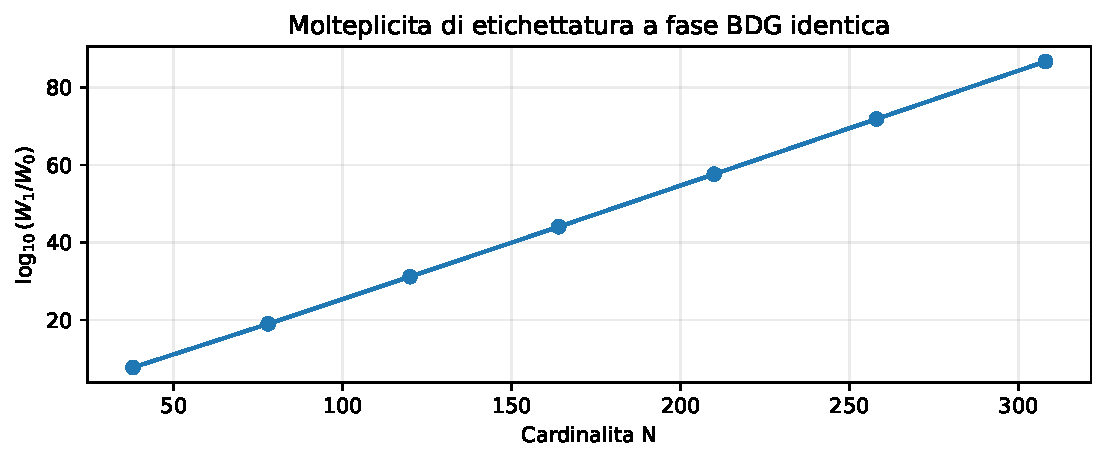
\includegraphics[width=0.76\linewidth]{R12BB_GW_NATURAL_LABEL_RATIO.pdf}
 \caption{Rapporto delle due molteplicit\`a naturali a uguale azione BDG. La crescita dipende dalla convenzione di conteggio e non certifica un effetto gravitazionale.}
\end{figure}

\clearpage
\subsection*{GW.2 --- Controllo dell'intera famiglia e limiti di identificazione}
L'illustrazione $C_0,C_1$ \emph{non} giustifica un'affermazione di dominanza globale: per esempio a $m=3$, $N=120$, il ramo $b_0=1$ contiene soltanto circa $1.0621\%$ della somma dei conteggi $W_{\rm nat}$ sull'intera famiglia dei 16 causal set, perche gli altri blocchi contribuiscono con un'enorme molteplicit\`a di intrecci fra catene. L'audit somma esattamente
\begin{equation}
 \mathcal W_m^{\rm nat}=\sum_{\sigma\in\{0,1\}^{m+1}}W_m(\sigma),\quad
 f_m=\frac{\sum_{\sigma:b_0=1}W_m(\sigma)}{\mathcal W_m^{\rm nat}}
 \quad(m=1,\ldots,7),\tag{GW.9}
\end{equation}
con \emph{aritmetica intera} e senza campionare soltanto i casi favorevoli. La fase del sottosettore e comune, quindi una somma a peso naturale uniforme sui \emph{poset naturalmente etichettati} avrebbe, come identita diagnostica, $\mathcal W_m^{\rm nat}\exp[i\theta(N-1)]$; cio \textbf{non} costituisce una somma fisica giustificata. Non si dispone di una misura di crescita quantistica covariante che richieda tale convenzione.

\textbf{Verifiche indipendenti.} Dopo la costruzione esplorativa di GW.1--GW.9, il protocollo congelato \texttt{R12BB\_GW\_PROTOCOL\_V080.json} viene verificato da due implementazioni: (i) quoziente fattoriale delle componenti, (ii) intercalazione ricorsiva dei blocchi tramite coefficienti binomiali e quoziente per automorfismi. Esse concordano \emph{byte per byte} sui $508$ membri di $m=1,\ldots,7$ e su tutte le statistiche dell'azione (incluse le firme di non-isomorfismo). Un terzo controllo indipendente esaustivo assegna davvero le etichette naturali e deduplica le matrici d'ordine per \emph{44 partizioni in catene} con $N\le7$; i valori coincidono esattamente. I risultati sono interi esatti; il grafico usa soltanto $\log_{10}$ per visualizzazione.

\textbf{Portata fisica.} La descrizione con etichette di nascita non stabilisce che le etichette siano gradi di liberta fisici: la covarianza discreta richiede cautela nel loro conteggio. Anche il fattore $1/|\mathrm{Aut}|$ e un'opzione di state sum, non un principio imposto dai test. La differenza enorme fra convenzioni dimostra la sensibilita dell'\emph{entropia di rappresentazione}, non che una delle geometrie domini la gravita quantistica. Una misura fisica deve essere definita indipendentemente e verificata con normalizzazione, covarianza, positivita, composizione, risposta e limite geometrico appropriati. Questo problema e discusso, a livello di state sum e fattori di simmetria, nella panoramica di Surya (\href{https://doi.org/10.1007/s41114-019-0023-1}{Living Reviews in Relativity, 2019}) e in analisi dei path sum di causal set (\href{https://doi.org/10.1007/s10714-024-03281-1}{Carlip, 2024}).

\textbf{Decisione R12bb-GW:} risultato matematico esatto PASS per il problema di conteggio e la famiglia fissata; \textbf{misura gravitazionale fisica NON SELEZIONATA}. Non vengono derivati QBC operatoriale non commutativa, azione gravitazionale dinamica 4D o $H(z)$. \textbf{R12bc NON APERTO; R12as fisico NON AUTORIZZATO; R13 BLOCCATO.}

\clearpage
\section*{Appendice R12bb-UC --- Coerenza proiettiva e pesi di conteggio}
\textbf{Obiettivo.} Dopo la degenerazione della fase BDG (v0.78--v0.79) e il confronto tra molteplicit\`a di rappresentazione (v0.80), chiediamo se una prescrizione di conteggio normalizzata indipendentemente a ciascun numero di elementi possa gi\`a definire una legge di crescita stocastica covariante. Non modifichiamo $Q_4$ e non introduciamo nuovi coefficienti fisici. Il controllo riguarda la \emph{coerenza di misure classiche finite}, non la determinazione dell'ampiezza gravitazionale.

Sia $\mathcal P_n$ l'insieme delle classi di isomorfismo dei causal set di $n$ elementi, e sia $W(C)$ il numero delle loro relazioni naturalmente etichettate, gi\`a distinto dagli automorfismi nella v0.80. Per una misura classica $q_n$ sulle classi, la \emph{covarianza discreta dei cammini} richiede che ciascuna delle $W(C)$ storie di nascita inequivalenti che raggiungono $C$ abbia la stessa probabilit\`a $q_n(C)/W(C)$. Indichiamo con $\pi_n$ il taglio che elimina l'ultimo nato nella storia etichettata. La coerenza proiettiva impone
\begin{equation}
\boxed{q_n(C)=\sum_{\substack{h\in\mathcal H_{n+1}\\[1pt] [\pi_n(h)]=C}}
\frac{q_{n+1}([h])}{W([h])}.}\tag{UC.1}
\end{equation}
Si tratta di una condizione necessaria alle probabilit\`a cilindriche del processo di crescita. Il prefisso a $n$ nascite \emph{non \`e}, di per s\'e, un osservabile covariante sulle storie infinite.

\subsection*{UC.1 --- Controesempio esaustivo a tre elementi}
Esistono due classi a $n=2$ (catena e anticatena) e cinque a $n=3$. I conteggi esatti delle storie naturalmente etichettate sono:
\begin{center}\small
\begin{tabular}{lrrrr}
\toprule
Classe a $n=3$ & $W(C)$ & $|\mathrm{Aut}(C)|$ & Prefisso catena & Prefisso anticatena\\
\midrule
Anticatena $A_3$ &1&6&0&1\\
Catena $K_3$ &1&1&1&0\\
Due minimi sotto un massimo (V)&1&2&0&1\\
Un minimo sotto due massimi ($\Lambda$)&1&2&1&0\\
Un legame e un isolato ($K_2\sqcup A_1$)&3&1&1&2\\
\bottomrule
\end{tabular}
\end{center}
Ponendo $q_3(C)=1/5$ per tutte le cinque classi e $q_2(K_2)=1/2$, l'equazione UC.1 per la catena richiederebbe
\begin{equation}
\boxed{q_3(\pi_2^{-1}K_2)=\frac15+\frac15+\frac{1}{3}\frac15
=\frac7{15}\ne\frac12=q_2(K_2).}\tag{UC.2}
\end{equation}
Pertanto \textbf{una distribuzione uniforme sulle classi non isomorfe a ogni $n$ non pu\`o essere la legge marginale di un'unica crescita stocastica normalizzata e generalmente covariante}. Non \`e una restrizione universale sulle misure quantistiche.

\clearpage
\subsection*{UC.2 --- Tre convenzioni, stesso problema}
Per ogni $n$ abbiamo fissato, prima dei controlli indipendenti, tre convenzioni \emph{diagnostiche}, ciascuna normalizzata separatamente:
\begin{equation}
q_n^{\mathrm{classi}}(C)\propto1,\qquad
q_n^{\mathrm{etichette}}(C)\propto W(C),\qquad
q_n^{\mathrm{sym}}(C)\propto\frac1{|\mathrm{Aut}(C)|}.
\tag{UC.3}
\end{equation}
Definiamo $D_{n\to n+1}=\frac12\sum_{C\in\mathcal P_n}|q_n(C)-\pi_{n\sharp}q_{n+1}(C)|$. Si ottiene con aritmetica razionale esatta:
\begin{center}\small
\begin{tabular}{lccc}
\toprule
Pesi classi $q_n(C)$ & $D_{2\to3}$ & $D_{3\to4}$ & $D_{4\to5}$\\
\midrule
Classi uniformi & $1/30$ & $29/320$ & $68287/582120$\\
Etichette naturali uniformi & $1/14$ & $11/140$ & $23/238$\\
Inverso automorfismi & $5/57$ & $2198/20805$ & $2826542/23782451$\\
\bottomrule
\end{tabular}
\captionof{table}{Tutte le distanze sono positive, dunque nessuna convenzione produce queste marginali di crescita quando i livelli sono normalizzati indipendentemente.}
\end{center}
Gi\`a a tre elementi, le probabilit\`a del prefisso catena sono rispettivamente $7/15$, $3/7$, $11/19$, mentre al livello due risultano $1/2$, $1/2$, $2/3$. Si escludono perci\`o tre \emph{prescrizioni di conteggio ingenuo}, non tutte le funzioni di peso possibili.

\begin{figure}[H]\centering
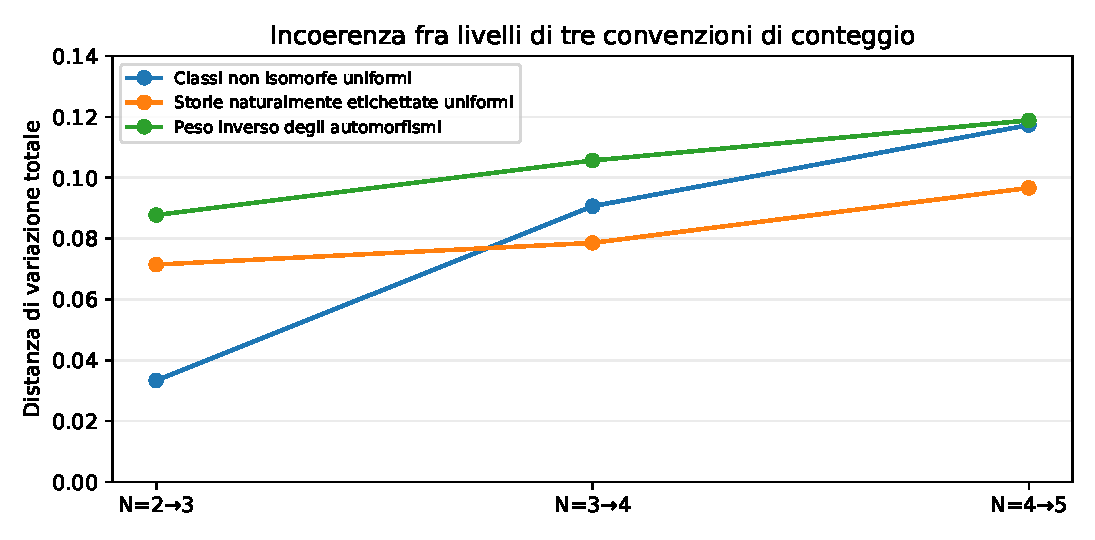
\includegraphics[width=0.87\linewidth]{R12BB_UC_PROJECTIVITY_DEFECT.pdf}
\caption{Distanza proiettiva dei tre schemi diagnostici: il livello zero sarebbe richiesto da una singola legge stocastica covariante, ma non \`e raggiunto da nessuno dei tre schemi.}
\end{figure}

La differenza $1/30$ della UC.2 \`e anche la \emph{minima} distanza di variazione totale necessaria per correggere $q_3$ mantenendo $q_2$ uniforme: la funzione che indica la quota di storie con prefisso catena appartiene a $[0,1]$, quindi la variazione della sua media non pu\`o superare la distanza totale. La soglia \`e raggiungibile, ad esempio, trasferendo massa $1/30$ dall'anticatena $A_3$ alla catena $K_3$, lasciando invariati gli altri tre pesi. Questa \`e una correzione matematica della legge \emph{finita}, non una misura fisica proposta.

\clearpage
\subsection*{UC.3 --- Controllo positivo senza parametri nuovi}
Per evitare di trasformare la contraddizione precedente in un impossibile divieto generale, verifichiamo la \emph{percolazione transitiva} storica a $p=1/2$. Per ogni storia naturalmente etichettata $C$ di $n$ elementi, $R(C)$ e il numero di coppie comparabili e $c(C)$ il numero di relazioni di copertura. Le maschere di archi primitivi che producono $C$ sono esattamente $2^{R-c}$, perch\'e tutti i link devono essere presenti e gli archi transitivamente ridondanti sono opzionali. Dunque
\begin{equation}
\boxed{P_n(C)=2^{R(C)-c(C)-\binom n2}.}\tag{UC.4}
\end{equation}
Se il nuovo elemento nasce con il downset degli antenati $D$, $w=|D|$ e $m=|\max D|$, la probabilit\`a elementare della transizione \`e $2^{w-m-n}$. Tutte le transizioni sommano a uno, e il prodotto di queste probabilit\`a coincide con UC.4; la formula dipende da statistiche intrinseche del poset, quindi \`e compatibile con la covarianza discreta. Al livello tre, le cinque classi hanno probabilit\`a $1/8,1/4,1/8,1/8,3/8$ nell'ordine della tabella UC.1. Ne segue
\begin{equation}
\frac14+\frac18+\frac13\,\frac38=\frac12,
\tag{UC.5}
\end{equation}
come richiesto dalla marginale di due elementi. Il confronto esatto dei tre metodi (conteggio delle maschere primitive, formula delle cover e prodotti di downset) verifica tutte le $407$ storie naturalmente etichettate con $1\le n\le5$ e le proiezioni $n+1\to n$.

\textbf{Audit indipendente.} Il protocollo UC fu congelato dopo la derivazione UC.2 e \emph{prima} dei risultati indipendenti ai livelli quattro e cinque (SHA-256 registrato nel recovery). Due implementazioni separate hanno generato le storie mediante (i) tutte le maschere di archi primitivi e chiusura transitiva, (ii) crescita per downset e identificazione tramite isomorfismo; entrambe distinguono $357$ relazioni naturalmente etichettate e $63$ classi a $n=5$, e producono risultati JSON \emph{byte-identici}. Il controllo positivo $p=1/2$ \`e stato aggiunto con amendment esplicito \emph{dopo} quei risultati, e non ne modifica lo statuto. La letteratura di riferimento \`e Rideout--Sorkin, \emph{Classical sequential growth dynamics for causal sets}, \href{https://doi.org/10.1103/PhysRevD.61.024002}{Phys. Rev. D 61, 024002} (1999/2000).

\textbf{Decisione R12bb-UC.} Le tre prescrizioni di conteggio normalizzate separatamente a ogni livello \textbf{FAIL} per la coerenza proiettiva sotto la covarianza discreta delle storie; il controllo positivo \`e \textbf{PASS}. La coerenza pu\`o essere ottenuta con una dinamica non uniforme, ma \emph{non} ne deriva una selezione della misura gravitazionale quantistica. Il calcolo non modifica l'azione BDG, non impone QBC operatoriale non commutativa, non ottiene gravit\`a emergente 4D o $H(z)$. \textbf{R12bc NON APERTO; R12as fisico NON AUTORIZZATO; R13 BLOCCATO.}

\clearpage
\section*{Appendice R12bb-AP --- Ostacolo alla normalizzazione di una fase BDG scalare}
\textbf{Domanda.} Dopo il fallimento delle pesature classiche per livello (UC, v0.81), ci chiediamo se una fase di azione gravitazionale sia sufficiente a ottenere una famiglia coerente di ampiezze, a meno di un \emph{solo fattore globale per taglia}. L'azione e i parametri storici sono immutati. Il risultato estende il controllo di fase della v0.61 a \emph{ogni angolo reale}, anziche soltanto all'accoppiamento diagnostico allora considerato.

Scriviamo l'indice discreto BDG quadridimensionale
\begin{equation}
 Q_4(C)=N-N_0+9N_1-16N_2+8N_3,\quad z=e^{i\theta},\quad |z|=1,\quad \theta\in\mathbb R,\tag{AP.1}
\end{equation}
con $N_j$ numero di intervalli con $j$ elementi interni. Siano $A_2$ l'anticatena e $K_2$ la catena di due elementi. Confrontiamo le due prescrizioni scalari \emph{separate}
\begin{equation}
 \alpha_n^{(\mathrm U)}(C)=c_nz^{Q_4(C)},\qquad
 \alpha_n^{(\mathrm P)}(C)=c_n P_{1/2,n}(C)z^{Q_4(C)},\qquad c_n\ne0,\tag{AP.2}
\end{equation}
dove $c_n$ dipende soltanto da $n$ e $P_{1/2,n}$ e la percolazione transitiva classica sui poset naturalmente etichettati. L'additivita delle ampiezze sui cilindri richiede, per \emph{ogni} genitore $C$,
\begin{equation}
 \alpha_n(C)=\sum_{C'\succ C}\alpha_{n+1}(C').\tag{AP.3}
\end{equation}
Dividendo per $\alpha_n(C)$ emerge una condizione necessaria: a una taglia fissata, la somma dei pesi relativi di tutti i figli deve essere \emph{uguale per ogni genitore}. In caso contrario non puo esistere un unico rapporto $c_n/c_{n+1}$.

I quattro downset dell'anticatena $A_2$ producono salti di indice $\Delta Q_4=(1,0,0,-1)$; i tre della catena $K_2$ producono $(1,0,9)$. I coefficienti elementari della percolazione $p=1/2$ sono rispettivamente $(1/4,1/4,1/4,1/4)$ e $(1/4,1/4,1/2)$. Gli istogrammi completi sono
\begin{center}\small
\begin{tabular}{lccc}
\toprule
Genitore & $Q_4$ & Somma fase sola $F^{(\rm U)}$ & Somma con prior $F^{(\rm P)}$\\
\midrule
$A_2$ & 2 & $z+2+z^{-1}$ & $(z+2+z^{-1})/4$\\
$K_2$ & 1 & $z+1+z^9$ & $(z+1+2z^9)/4$\\
\bottomrule
\end{tabular}
\end{center}
I conteggi comprendono le continuazioni \emph{naturalmente etichettate}, senza considerare le etichette un osservabile fisico; la coerenza cilindrica e una condizione interna alla rappresentazione tramite storie di nascita.

\clearpage
\subsection*{AP.1 --- Due ostacoli esatti per tutte le fasi reali}
Per la \emph{fase sola} $F_{A_2}^{(\rm U)}=F_{K_2}^{(\rm U)}$ implica
\begin{equation}
 z^{10}=1+z.\tag{AP.4}
\end{equation}
La condizione $|z|=1$ darebbe $|1+z|=1$, ossia $z+z^{-1}=-1$ e quindi $z^2+z+1=0$. Ma allora $z^3=1$ con $z\ne1$, per cui $z^{10}=z$, incompatibile con AP.4. \textbf{Non esiste alcuna fase unitaria risolutiva}, neppure $z=1$: a fase nulla il numero dei figli e 4 contro 3.

Per l'\emph{ansatz che moltiplica la prior classica} $F_{A_2}^{(\rm P)}=F_{K_2}^{(\rm P)}$ implica invece
\begin{equation}
 2z^{10}=1+z.\tag{AP.5}
\end{equation}
Prendendo il modulo si ottiene $2=|1+z|$. Con $|z|=1$ l'uguaglianza triangolare vale soltanto per $\boxed{z=1}$. In quel caso $z^{Q_4(C)}=1$ per ogni indice intero, e resta semplicemente la percolazione proiettivamente coerente della v0.81. Ogni fase \emph{non banale} e esclusa \emph{solo per questo ansatz di twist scalare, con fattori globali per livello}.

\begin{figure}[H]\centering
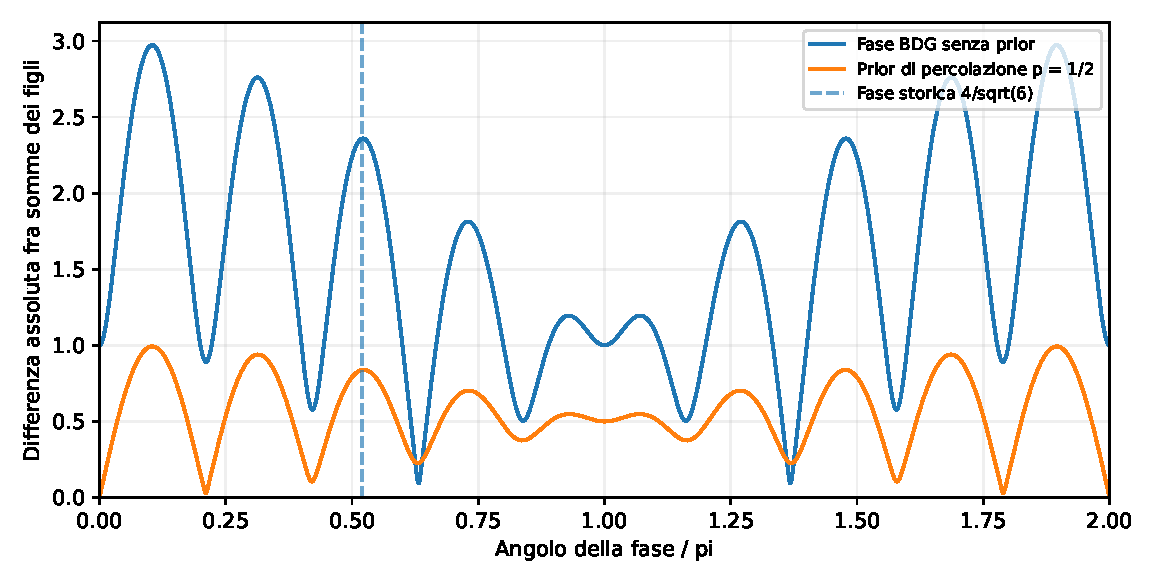
\includegraphics[width=0.85\linewidth]{R12BB_AP_GLOBAL_NORMALIZER_GAP.pdf}
\caption{Modulo della differenza fra le somme dei figli di $A_2$ e $K_2$. Il grafico e diagnostico; l'impossibilita segue dalle identita AP.4--AP.5 e non dalla scansione degli angoli.}
\end{figure}
Per il valore storico non modificato $\theta=4/\sqrt6$, i due moduli sono, rispettivamente, circa $2.3586305592$ e $0.8385474686$. La loro grandezza non viene usata per scegliere un'accoppiamento.

\clearpage
\subsection*{AP.2 --- Controlli indipendenti, provenienza e limiti fisici}
La dimostrazione AP.4--AP.5 e stata ottenuta \emph{esplorativamente}; il protocollo di audit AP (nel recovery) e stato congelato \emph{dopo} il doppio controllo pilota a $n=2$, ma \emph{prima} dell'ulteriore holdout sui genitori di tre e quattro elementi. Non si rivendica una scoperta prospettica cieca.

\begin{center}\small
\begin{tabular}{p{9.2cm}r}
\toprule
Controllo deterministico & Esito\\
\midrule
Due metodi distinti sui quattro/tre downset di $A_2,K_2$ & $2/2$ PASS\\
Genitori naturalmente etichettati a $n=3$ e $n=4$ & $7+40=47$\\
Continuazioni naturali identificate nell'holdout & $40+357=397$\\
Istogrammi dei salti $\Delta Q_4$ e pesi Bernoulli razionali, confrontati per genitore & $47/47$ PASS\\
Normalizzazione della prior senza fase per tutti i genitori holdout & $47/47$ PASS\\
\bottomrule
\end{tabular}
\captionof{table}{Programmi distinti: crescita mediante ideali di ordine e enumerazione delle configurazioni primitive Bernoulli con chiusura transitiva; output JSON confrontati byte per byte.}
\end{center}
\textbf{Limite esatto del teorema.} AP.4--AP.5 sono \emph{condizioni necessarie} per due famiglie di ampiezze scalari specificate da AP.2. Non escludono ampiezze di transizione non fattorizzabili, una struttura a operatori non commutanti, una misura quantistica covariante indipendentemente motivata, o la possibilita di usare l'azione BDG in un vero path integral dopo aver definito la misura. Non identificano una dinamica gravitazionale 4D e non producono un $H(z)$ autonomo.

\textbf{Relazione con i risultati precedenti.} La v0.61 gia dimostrava il fallimento della fase BDG moltiplicata per percolazione per l'angolo storico e la difformita di una riparazione locale. Qui si formalizza la \emph{restrizione esatta di tutto il cerchio delle fasi} sotto la normalizzazione globale, si esplicita la differenza tra prior uniforme e prior stocastica, e si conserva il controllo positivo $z=1$ (privo di fase). Per la cornice di crescita classica si veda Rideout--Sorkin, \href{https://doi.org/10.1103/PhysRevD.61.024002}{Phys. Rev. D 61 (2000), 024002}; per l'azione BDG e la soppressione nei path sum, Carlip, \href{https://doi.org/10.1007/s10714-024-03281-1}{Gen. Rel. Grav. 56 (2024), 95}.

\textbf{Decisione R12bb-AP:} no-go matematico per i due ansatz scalari (PASS); selezione della misura fisica \textbf{NON OTTENUTA}. \textbf{R12bc NON APERTO; R12as fisico NON AUTORIZZATO; R13 BLOCCATO.}

\clearpage
\section*{Appendice R12bb-FH --- Ampiezze BDG a orizzonte finale fissato (v0.83)}
\textbf{Domanda e confine del test.} La v0.82 ha dimostrato che moltiplicare la percolazione transitiva $P_{1/2}$ per $z^{Q_4}$ e poi usare un solo normalizzatore per livello non fornisce coerenza cilindrica, salvo fase banale. Qui non si modifica ne il modello di crescita ne l'azione: si verifica una \emph{costruzione condizionata a un orizzonte finale $T$}, distinta da una legge locale e autonoma. Restano fissati
\[
 Q_4(C)=N-N_0+9N_1-16N_2+8N_3,\quad
 z=e^{i\theta},\quad \theta=4/\sqrt6.
\]
Ogni storia naturalmente etichettata $C_T$ ha peso razionale $P_{1/2,T}(C_T)$, comprensivo delle moltiplicita delle configurazioni primitive compatibili con la chiusura transitiva. Per $0\le n\le T$ e un prefisso $C_n$ si pone
\begin{equation}
 G_n^{[T]}(C_n;z)=\sum_{C_T:\,C_T|_n=C_n}P_{1/2,T}(C_T)z^{Q_4(C_T)},\qquad
 Z_T(z)=G_0^{[T]}(\varnothing;z),\qquad
 \nu_n^{[T]}(C_n)=\frac{G_n^{[T]}(C_n;z)}{Z_T(z)}.\tag{FH.1}
\end{equation}
I polinomi $G_n^{[T]}$ hanno coefficienti razionali esatti, e si sommano sui discendenti terminali senza introdurre alcun nuovo accoppiamento. La definizione e una \emph{pesatura complessa a condizione finale}, analoga al formalismo di trasformazione $h$ retrograda (non un ordinario condizionamento probabilistico positivo).

\textbf{Teorema FH-1 (coerenza a $T$ fissato).} Per ogni $T$ e ogni $n<T$ le ampiezze (FH.1) soddisfano
\begin{equation}
 \nu_n^{[T]}(C_n)=\sum_{C_{n+1}\succ C_n}\nu_{n+1}^{[T]}(C_{n+1}),\qquad
 \sum_{C_n}\nu_n^{[T]}(C_n)=1.\tag{FH.2}
\end{equation}
\emph{Dimostrazione.} Ogni storia terminale appartiene a uno e un solo cilindro figlio; la partizione delle somme finite che definiscono $G_n^{[T]}$ e esatta. L'azione e il prior dipendono dall'ordine parziale e non dalla scelta della etichettatura naturale, quindi l'ampiezza del prefisso e covariante rispetto alle rietichettature naturali di poset isomorfi. Sull'algebra finita di cilindri $D_T(A,B)=\nu_T(A)\overline{\nu_T(B)}$ e fortemente positivo di rango al piu uno: questa proprieta \emph{non} seleziona una misura gravitazionale.

Se $H_n^{[T]}(C)=G_n^{[T]}(C)/P_{1/2,n}(C)$ e non nullo, si possono anche scrivere transizioni complesse normalizzate
\begin{equation}
 \widehat t_n^{[T]}(C\to D)=P_{1/2}(D\mid C)\,
 \frac{H_{n+1}^{[T]}(D)}{H_n^{[T]}(C)},\qquad
 \sum_{D\succ C}\widehat t_n^{[T]}(C\to D)=1.\tag{FH.3}
\end{equation}
La condizione terminale e incorporata in $H_n^{[T]}$: \textbf{questa non e una legge di crescita senza orizzonte finale}. Le ampiezze complesse e la loro normalizzazione non sono probabilita classiche.

\clearpage
\subsection*{FH.1 --- Ostruzione esatta alla compatibilita fra orizzonti differenti}
Siano $A_2$ l'anticatena e $K_2$ la catena di due elementi. L'enumerazione analitica da n=2 a n=3 restituisce, prima della normalizzazione globale,
\begin{align}
 &G_2^{[2]}(A_2)=z^2/2,\qquad G_2^{[2]}(K_2)=z/2,\notag\\
 &G_2^{[3]}(A_2)=\frac{z+2z^2+z^3}{8},\qquad
 G_2^{[3]}(K_2)=\frac{z+z^2+2z^{10}}8.\tag{FH.4}
\end{align}
Il rapporto $\nu(K_2)/\nu(A_2)$ e uguale a $z^{-1}$ per $T=2$. Per essere lo stesso a $T=3$, dove i denominatori sono non nulli, dovrebbe annullarsi
\begin{equation}
 z\,(z+z^2+2z^{10})-(z+2z^2+z^3)
 =z(2z^{10}-1-z).\tag{FH.5}
\end{equation}
Con $|z|=1$, $2z^{10}=1+z$ impone $|1+z|=2$, e quindi soltanto $z=1$. \textbf{Ogni fase non banale impedisce che le normalizzazioni terminali a $T=2$ e $T=3$ definiscano lo stesso assegnamento di ampiezze sul taglio a due elementi.} Non e necessario esplorare o ritoccare $\theta$ per dimostrarlo.

\textbf{Denominatori a $\theta$ storico.} Il numero $i\,4/\sqrt6$ e algebrico non nullo: per il teorema di Hermite--Lindemann $z=e^{i4/\sqrt6}$ e trascendente. Ogni somma $G_n^{[T]}(C;z)$ relativa a un prefisso raggiungibile e un polinomio di Laurent \emph{non nullo} a coefficienti razionali non negativi, sicche non puo annullarsi in quel particolare $z$, a ogni $T$ finito. Ne segue che (FH.1) e (FH.3) sono ben definite per tutti i prefissi finiti raggiungibili al valore storico. Questo argomento non e una prova di convergenza per $T\to\infty$.

\begin{center}\small
\begin{tabular}{r r r r}
\toprule
$T$ & $|Z_T|$ & $\operatorname{Re}(\nu(K_2)/\nu(A_2))$ & $\operatorname{Im}(\nu(K_2)/\nu(A_2))$\\
\midrule
2 & 0.684778526 & -0.062156742 & -0.998066400\\
3 & 0.571402749 &  1.436982521 & -0.023178167\\
4 & 0.405705996 &  2.197930174 &  0.604231778\\
5 & 0.311191959 &  1.777406627 &  0.194762909\\
6 & 0.227988877 &  1.818281470 &  0.956489332\\
\bottomrule
\end{tabular}
\captionof{table}{Diagnostica a orizzonti piccoli $T=2,\dots,6$, con $\theta=4/\sqrt6$ fissato. Nessuna estrapolazione asintotica e autorizzata.}
\end{center}

\clearpage
\subsection*{FH.2 --- Audit indipendente e implicazioni}
\begin{figure}[H]\centering
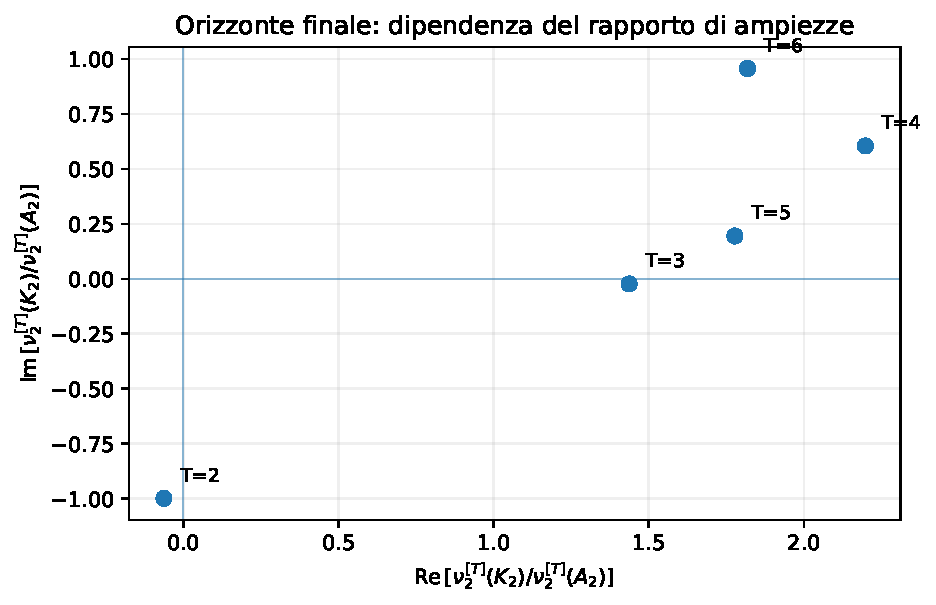
\includegraphics[width=0.71\linewidth]{R12BB_FH_HORIZON_WITNESS.pdf}
\caption{Rapporto fra le ampiezze dei due prefissi a $n=2$ per cinque diversi orizzonti finali. Ogni punto e una valutazione del corrispondente polinomio esatto. La figura non dimostra ne esclude un limite per $T\to\infty$.}
\end{figure}

\begin{center}\small
\begin{tabular}{p{10cm}r}
\toprule
Verifica eseguita su $T=2,\dots,6$ & Esito\\
\midrule
Confronto coefficienti di tutti i polinomi di Laurent, due algoritmi distinti & 5,706/5,706 PASS\\
Identita di partizione genitore-figli dentro ogni orizzonte & 476/476 PASS\\
Confronti su etichettature naturali isomorfe fino a $n\le5$ & 668/668 PASS\\
Normalizzazioni a $z=1$ su tutti i tagli finiti & 25/25 PASS\\
Conteggi terminali di poset naturalmente etichettati $T=2,3,4,5,6$ & 2, 7, 40, 357, 4,824\\
Controllo simbolico fra $T=2$ e $T=3$ & PASS (solo $z=1$)\\
\bottomrule
\end{tabular}
\end{center}
I due algoritmi non condividono il motore di generazione: il primo espande i \emph{downset} con moltiplicita primitive $2^{|D|-|\operatorname{Max}D|}$; il secondo enumera direttamente i $2^{\binom T2}$ insiemi di archi primitivi e applica la chiusura transitiva. La derivazione e il doppio confronto $T\le6$ precedono il congelamento del protocollo; la verifica successiva sulle classi di isomorfismo e il controllo positivo a $z=1$ sono registrati separatamente. Nessun risultato e stato scartato.

\textbf{Implicazione scientifica.} A orizzonte finito il condizionamento terminale permette una famiglia esatta, coerente e con forte positivita del funzionale di decoerenza di rango uno. Tuttavia \emph{non seleziona il confine futuro $T$} e fallisce la compatibilita immediata fra $T=2$ e $T=3$ per $z\ne1$. Il possibile limite $T\to\infty$ non e stato analizzato; eventuali scelte di confine, regolarizzazione e continuita richiederebbero un principio microfisico esterno. Non abbiamo derivato una QBC operatoriale non commutativa, una misura BDG fisica, una dinamica 4D o $H(z)$.

\textbf{Fonti matematiche.} Per la trasformazione $h$ positiva ordinaria e il condizionamento al tempo terminale: \href{https://mathworld.wolfram.com/Doobh-Transform.html}{MathWorld, Doob $h$-Transform}; qui il peso e \emph{complesso}, e non si introduce una probabilita classica. Per Hermite--Lindemann: \href{https://encyclopediaofmath.org/wiki/Lindemann--Weierstrass_theorem}{Encyclopedia of Mathematics, Lindemann--Weierstrass theorem}. La BDG e la percolazione storiche rimangono quelle delle versioni precedenti.

\textbf{Stato R12bb-FH:} $\textsf{FINITE-HORIZON-MATH-PASS}$ con $\textsf{CROSS-HORIZON-FAIL}$ per la fase non banale. \textbf{R12bc NON APERTO; R12as fisico NON AUTORIZZATO; R13 BLOCCATO.}

\clearpage
\section*{Appendice R12bb-CB --- Fase BDG come cobordo e indeterminazione della misura (v0.84)}
\textbf{Problema.} Le versioni v0.82 e v0.83 hanno distinto una normalizzazione scalare per livello (insufficiente per fasi non banali) da una trasformazione condizionata all'orizzonte futuro (consistente soltanto a orizzonte fissato). Qui sottoponiamo a controllo una possibilita ancora piu ampia: consentire un compensatore complesso \emph{arbitrario dipendente dall'intera storia parziale}. Il risultato e un limite alla capacita selettiva di questa liberta, \textbf{non} una proposizione secondo cui l'azione gravitazionale BDG sia fisicamente inutile.

Fissiamo ancora la percolazione transitiva classica $P=P_{1/2}$, l'indice intero
\[
 Q_4(C)=N-N_0+9N_1-16N_2+8N_3,
 \qquad z=e^{i\theta},\quad \theta=4/\sqrt6.
\]
Consideriamo la transizione elementare $p(C,D)=P(D\mid C)$ fra un prefisso naturalmente etichettato $C$ e un figlio $D$. Se $h_n(C)\neq0$ e un compensatore, la transizione corretta e
\begin{equation}
 \widehat t_h(C,D)=p(C,D)\,z^{Q_4(D)-Q_4(C)}
 \frac{h_{n+1}(D)}{h_n(C)}.\tag{CB.1}
\end{equation}
\textbf{Teorema CB-1 (liberta di cobordo).} Sia $F$ una funzione complessa limitata sulle storie infinite, con $\mathbb E_P F\neq0$. Poniamo $m_n(C)=\mathbb E_P[F\mid C_n=C]$ e assumiamo $m_n(C)\neq0$ sui prefissi raggiungibili. Allora, scegliendo $h_n(C)=z^{-Q_4(C)}m_n(C)$, si ottiene \emph{esattamente}, per ogni $z\neq0$,
\begin{equation}
 \boxed{\widehat t_h(C,D)=p(C,D)\frac{m_{n+1}(D)}{m_n(C)},
 \qquad \sum_{D\succ C}\widehat t_h(C,D)=1.}\tag{CB.2}
\end{equation}
Le ampiezze cilindriche cosi prodotte sono
\begin{equation}
 \boxed{\nu_n(C)=P_n(C)\frac{m_n(C)}{\mathbb E_P F},\qquad
 \nu(E)=\frac{\mathbb E_P[F\mathbf1_E]}{\mathbb E_P F}.}\tag{CB.3}
\end{equation}
\emph{Dimostrazione.} L'esponente di $z$ in CB.1 diviene $(Q_4(D)-Q_4(C))-Q_4(D)+Q_4(C)=0$. L'identita di martingala $\sum_D p(C,D)m_{n+1}(D)=m_n(C)$ fornisce la normalizzazione. Il prodotto telescopico delle transizioni fornisce CB.3. Poiche $F$ e limitata, CB.3 definisce una misura complessa sigma-additiva di variazione totale finita. Il funzionale $\mathcal D(A,B)=\nu(A)\overline{\nu(B)}$ e fortemente positivo e ha rango al piu uno. \emph{Nessuna di queste condizioni sceglie $F$.}

\textbf{Caso di controllo:} per $F=1$ abbiamo $m_n=1$, $h_n=z^{-Q_4(C)}$ e $\widehat t_h=p(C,D)$. Quindi l'intera fase esplicitamente introdotta in CB.1 viene compensata, pur rispettando tutte le normalizzazioni. Una correzione priva di un principio fisico indipendente non rende operativa l'azione.

\clearpage
\subsection*{CB.1 --- Un esempio complesso su un evento infinito covariante}
Come \textbf{testimone matematico, non come misura gravitazionale proposta}, scegliamo $E_2$ = ``la storia infinita contiene almeno due elementi minimi'' e $F=1+i\mathbf1_{E_2}$. L'evento e definito solo dall'ordine causale, dunque e covariante. Ogni nascita quando esistono $j\ge1$ elementi precedenti e un nuovo minimo se e solo se nessuno dei $j$ collegamenti primitivi e presente, evento di probabilita $2^{-j}$, indipendente per nascita. Ne segue
\begin{equation}
 p_*:=P(E_2)=1-\prod_{j=1}^{\infty}(1-2^{-j})
 =0.7112119049133975787\ldots.\tag{CB.4}
\end{equation}
Se $C_n$ contiene gia almeno due minimi, $g_n(C_n)=P(E_2\mid C_n)=1$; se contiene esattamente un minimo, per $n\ge1$,
\begin{equation}
 g_n(C_n)=1-\prod_{j=n}^{\infty}(1-2^{-j}),\qquad
 m_n(C_n)=1+i\,g_n(C_n).\tag{CB.5}
\end{equation}
Tutti gli $m_n$ sono non nulli. La misura complessa infinita, definita \emph{senza introdurre $\theta$ nei pesi effettivi}, assegna
\begin{align}
 &\nu(E_2)=\frac{(1+i)p_*}{1+ip_*},\qquad
 \nu(E_2^c)=\frac{1-p_*}{1+ip_*},\notag\\
 &\mu(E_2)=\frac{2p_*^2}{1+p_*^2}\simeq0.671822099,\qquad
 \mu(E_2^c)=\frac{(1-p_*)^2}{1+p_*^2}\simeq0.055384065,\notag\\
 &I_2(E_2,E_2^c)=\frac{2p_*(1-p_*)}{1+p_*^2}
 \simeq0.272793837>0.\tag{CB.6}
\end{align}
In effetti $\mu(E_2)+\mu(E_2^c)+I_2=\mu(\Omega)=1$: la misura quantistica non e una probabilita additiva. L'interferenza e \emph{autentica per questa misura complessa illustrativa}, ma non e attribuibile alla fase BDG, cancellata in CB.2.

\begin{figure}[H]\centering
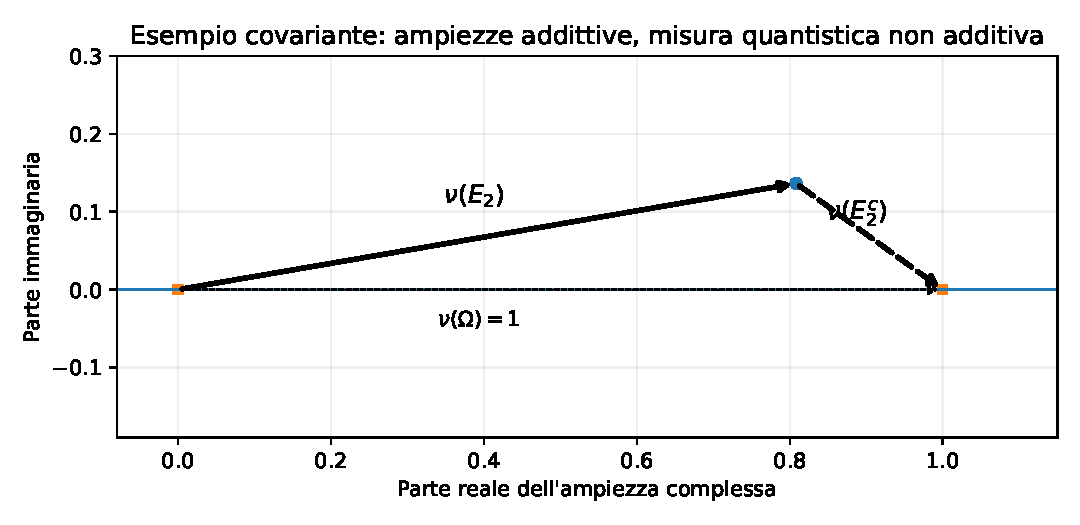
\includegraphics[width=0.78\linewidth]{R12BB_CB_COMPLEX_EVENT.pdf}
\caption{Ampiezze complesse dell'evento covariante $E_2$ e del complemento. I vettori sommano a uno, mentre i moduli quadratici non sono additivi. Illustrazione di una densita scelta per controesempio, non di una legge cosmologica.}
\end{figure}

Il prodotto razionale troncato ai primi 64 fattori certifica $p_*$ in un intervallo di larghezza non superiore a $2^{-64}$, mediante la somma geometrica delle code omesse. Questo limite riguarda il calcolo dell'\emph{esempio} e non fornisce alcuna selezione microfisica dei coefficienti.

\clearpage
\subsection*{CB.2 --- Due motori indipendenti e decisione fisica}
Per verificare le identita di base senza trattare $z$ come numero floating point, e stato fissato un taglio di \emph{verifica} $M=12$ solo per $P(E_2\text{ entro }M\mid C_n)$, con $n\le6$. Ogni valore e razionale; la cancellazione della fase viene controllata con la \emph{identita intera} $\Delta Q_4-Q_4(D)+Q_4(C)=0$, valida per ogni $z\neq0$. Le formule analitiche CB.2--CB.6 non dipendono dal taglio $M$.

\begin{center}\small
\begin{tabular}{p{10.4cm}r}
\toprule
Controllo & Risultato\\
\midrule
Poset naturalmente etichettati $n=0,\ldots,6$ & $1,1,2,7,40,357,4824$\\
Confronto diretto fra i due ledger esatti (tutte le storie) & $5232/5232$ PASS\\
Armonicita condizionale e normalizzazione su tutti i genitori $n<6$ & $408/408$ PASS\\
Cancellazione dell'esponente BDG per le transizioni distinte & $5231/5231$ PASS\\
Normalizzazione e compatibilita delle ampiezze complesse finite & PASS\\
Certificato razionale per l'evento infinito $E_2$ (64 fattori) & errore $\le2^{-64}$ su $p_*$\\
\bottomrule
\end{tabular}
\end{center}
Il primo motore enumera \emph{tutte} le maschere Bernoulli primitive e applica la chiusura transitiva; il secondo costruisce i poset aggiungendo downset e calcolando le molteplicit\`a $2^{|D|-|\max D|}$. I programmi non condividono il motore di enumerazione. I ledger hanno la medesima impronta SHA-256, e il replay e eseguibile dal pacchetto estratto. La scelta del testimone e la derivazione erano esplorative; il protocollo CB e stato congelato \emph{prima} della validazione computazionale indipendente, non prima della scoperta.

\textbf{Interpretazione e limiti.} CB.1--CB.3 dimostrano che una classe \emph{troppo libera} di compensatori rende formalmente compatibile qualsiasi fase del tipo $z^{\Delta Q_4}$ con misure anche molto diverse: l'azione e inserita come \emph{cobordo moltiplicativo} e poi rimossa. Questa non e un'obiezione alla BDG nel path integral con una misura specificata e vincoli fisici, ma una \textbf{critica all'uso della sola normalizzazione come criterio selettivo}. Occorrono condizioni indipendenti sulla natura di $h$: causalita quantistica, localita, struttura di stato e limite gravitazionale continuo. L'esempio $F=1+i\mathbf1_{E_2}$ utilizza un evento infinito futuro e non e una proposta fisica di dinamica autonoma.

\textbf{Fonti e provenienza.} Il formalismo delle trasformazioni armoniche positive e standard (\href{https://mathworld.wolfram.com/Doobh-Transform.html}{Doob $h$-transform}); la distinzione della misura quantistica e del suo funzionale di decoerenza e discussa in \href{https://doi.org/10.1007/s41114-019-0023-1}{Surya, Living Reviews in Relativity (2019)}. Il presente calcolo e un audit della liberta di cobordo nel \emph{nostro} benchmark fissato, non una nuova teoria gravitazionale.

\textbf{Decisione R12bb-CB:} identita di compensazione e controesempio covariante verificati come matematica; \textbf{misura fisica NON SELEZIONATA}. \textbf{R12bc NON APERTO; R12as fisico NON AUTORIZZATO; R13 BLOCCATO.}

\clearpage
\section*{Appendice R12bb-SB --- Bell causality degli spettatori e liberta residua della misura (v0.85)}
\textbf{Domanda dopo v0.84.} Una correzione dipendente arbitrariamente dalla storia puo cancellare la fase BDG e produrre transizioni normalizzate: quali compensatori vengono invece esclusi da un criterio causale indipendente? Usiamo qui il \emph{rapporto fra transizioni senza spettatori} della crescita \textbf{classica} di Rideout--Sorkin. Ne verifichiamo la trasposizione algebrica a \emph{ampiezze complesse scalari non nulle}, \textbf{senza identificarla con la quantum Bell causality operatoriale}. La prior resta la percolazione $P_{1/2}$; i coefficienti dell'indice BDG e la fase storica $z=e^{i4/\sqrt6}$ non cambiano.

\textbf{Famiglia analitica, non ricerca parametrica.} Indicando con $M_n(C)$ il numero di elementi minimi, ogni nascita di un nuovo minimo dopo $j\ge1$ elementi ha, sotto $P_{1/2}$, probabilita indipendente $2^{-j}$. Pertanto $M_\infty=1+\sum_{j\ge1}I_j$ e finito quasi certamente. Per \emph{tutti} gli $u$ con $|u|=1$, $u\ne-1$, definiamo
\begin{equation}
 F_u=u^{M_\infty-1},\qquad B(u)=\mathbb E_{P_{1/2}}F_u
 =\prod_{j=1}^{\infty}\left[1+(u-1)2^{-j}\right],\qquad
 \nu_u(E)=\frac{\mathbb E_{P_{1/2}}[\mathbf 1_EF_u]}{B(u)}.
 \tag{SB.1}
\end{equation}
Il prodotto converge ed e non nullo: i fattori sono non nulli (per $|u|=1$ l'unico zero possibile e $u=-1$, al primo fattore), mentre la somma dei loro scarti da $1$ converge assolutamente. $|F_u|=1$ implica una misura complessa numerabilmente additiva di variazione totale finita. Anzi, per ogni evento misurabile,
\begin{equation}
 \boxed{|\nu_u|(E)=\frac{P_{1/2}(E)}{|B(u)|}.}\tag{SB.2}
\end{equation}
\textbf{Conseguenza geometrica:} tutti gli eventi nulli della percolazione, compresi gli eventi covarianti esclusi nei gate R12bb-PT e R12bb-PI, restano nulli in questa famiglia. Non segue alcuna nuova selezione di geometrie quadridimensionali.

\textbf{Kernel esatto.} Per ogni genitore $C_n$ con $n\ge1$ e ogni precursore/downset $D$, siano $w=|D|$ e $m=|\operatorname{Max}D|$. L'ampiezza della transizione e
\begin{equation}
 \boxed{T_u(C_n,D)=\frac{2^{w-m}\,u^{\mathbf1_{D=\varnothing}}}
 {2^n-1+u}.}\tag{SB.3}
\end{equation}
La nascita iniziale dall'insieme vuoto ha ampiezza $1$. La somma dei pesi di tutti i precursori non vuoti e $2^n-1$, perche enumera tutti gli insiemi non vuoti di bond primitivi; al precursore vuoto corrisponde $u$. Dunque la somma in (SB.3) e esattamente uno per ogni genitore, senza un fattore aggiustato ai dati. Per un $C_n$ con $R$ coppie comparabili, $c$ cover e $M$ minimi,
\begin{equation}
 \boxed{\nu_{u,n}(C_n)=\frac{2^{R-c}\,u^{M-1}}
 {\prod_{j=1}^{n-1}(2^j-1+u)},\qquad n\ge1.}\tag{SB.4}
\end{equation}
L'ampiezza dipende soltanto dagli invarianti del poset, e non dalla sua etichettatura naturale: covarianza discreta. Il funzionale $\mathcal D_u(A,B)=\nu_u(A)\overline{\nu_u(B)}$ e fortemente positivo, ma ha rango al piu uno. Le formule equivalgono a una sottoclasse \emph{gia nota} di crescita complessa, con $t_0=u$, $t_k=1$ per $k\ge1$.

\clearpage
\subsection*{SB.1 --- Test causale sugli spettatori e controesempio di v0.84}
Siano $D_1,D_2$ due precursori concorrenti. Nella trasposizione \emph{scalare} del criterio classico di Bell, il rapporto delle transizioni deve coincidere quando il genitore e ridotto a $D_1\cup D_2$. Con $w_j=|D_j|$, $m_j=|\operatorname{Max}D_j|$, abbiamo esattamente
\begin{equation}
 \boxed{\frac{T_u(C,D_1)}{T_u(C,D_2)}
 =2^{w_1-m_1-w_2+m_2}\,
 u^{\mathbf1_{D_1=\varnothing}-\mathbf1_{D_2=\varnothing}}.}\tag{SB.5}
\end{equation}
La destra non dipende dagli spettatori, quindi \textbf{il test Bell scalare e superato per tutta la famiglia}. Questo controllo e davvero restrittivo, non una tautologia della normalizzazione.

\textbf{Test negativo indipendente.} Nella v0.84 il peso illustrativo era $F=1+i\mathbf1_{E_2}$, con $E_2$ evento infinito ``almeno due elementi minimi''. Se il genitore ha un solo minimo, la funzione condizionale e $m_n=1+i r_n$, dove $r_n=1-\prod_{j=n}^{\infty}(1-2^{-j})$; dopo una nascita senza antenati $m=1+i$. Confrontiamo $D_0=\varnothing$ e $D_1=\{\text{un minimo}\}$: nel genitore singleton il rapporto risulta $(1+i)/(1+ir_2)$; nella catena a due elementi, il cui elemento superiore e spettatore, risulta $(1+i)/(1+ir_3)$. Poiche
\begin{equation}
 \boxed{r_2-r_3=\frac14\prod_{j=3}^{\infty}(1-2^{-j})>0,}
 \qquad\Rightarrow\qquad \text{Bell scalare: FAIL}.\tag{SB.6}
\end{equation}
Per un certificato razionale indipendente al cutoff dichiarato $M=6$ si trova $r_2=6619/16384$, $r_3=841/4096$, differenza $3255/16384>0$. \textbf{La covarianza dell'evento $E_2$ non basta, quindi, a garantire la causalita degli spettatori.}

\textbf{Classificazione soltanto nel settore dei minimi.} Supponiamo che la funzione armonica condizionale abbia la forma $m_n(C)=a_n g(M_n(C))$, con $a_n$ e $g(k)$ non nulli e $g$ indipendente da $n$. Dalla normalizzazione condizionale segue
\begin{equation}
 \frac{a_n}{a_{n+1}}=1-2^{-n}+2^{-n}\frac{g(M+1)}{g(M)}.\tag{SB.7}
\end{equation}
A dimensione $n$ sono realizzabili $M=1,\ldots,n$. Il lato sinistro non dipende da $M$, percio i rapporti $g(M+1)/g(M)$ coincidono per ogni $M$. Dunque $g(M)=g(1)u^{M-1}$: le sole soluzioni \emph{in questa famiglia fattorizzata} sono geometriche nel numero dei minimi. Non abbiamo classificato tutte le correzioni dipendenti dalla storia e non abbiamo scelto $u$ fisicamente.

\medskip
\subsection*{SB.2 --- Interferenza infinita certificata e audit esatto}
Per illustrare un membro \emph{non selezionato} della famiglia poniamo $u=i$. Siano $q=\prod_{j\ge1}(1-2^{-j})$ e $B=B(i)$ di (SB.1). Gli eventi covarianti complementari $E_2^c$ (un solo minimo) ed $E_2$ (almeno due minimi) hanno
\begin{align}
 \nu_i(E_2^c)&=q/B,\qquad \nu_i(E_2)=1-q/B,\notag\\
 \mu_i(E_2^c)&\simeq0.438445640,\qquad
 \mu_i(E_2)\simeq1.186574328,\notag\\
 I_2(E_2,E_2^c)&=1-\mu_i(E_2)-\mu_i(E_2^c)
 \simeq-0.625019968.\tag{SB.8}
\end{align}
Le ampiezze sommano a uno ma le misure quadratiche non sono probabilita classiche. Il troncamento a $64$ fattori di $q$ e $B$, con numeratori gaussiani razionali esatti, verifica $|B_{64}|>2/5$; il resto del prodotto induce $|\nu_i(E_2^c)-q_{64}/B_{64}|<11\cdot2^{-64}$ e l'errore di ciascuna misura quadratica e inferiore a $110\cdot2^{-64}$. \textbf{L'interferenza non discende dalla fase BDG}, gia eliminata per cobordo nella costruzione CB.2.

\begin{figure}[H]\centering
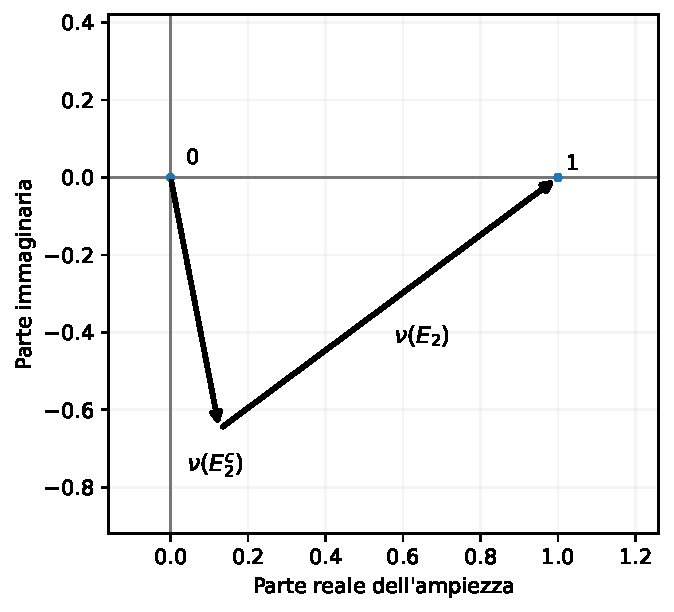
\includegraphics[width=0.70\linewidth]{R12BB_SB_COMPLEX_AMPLITUDES.pdf}
\caption{Somma vettoriale delle ampiezze complesse degli eventi $E_2^c$ ed $E_2$ nel membro $u=i$. Il valore non additivo della misura e un esempio matematico, non una stima cosmologica.}
\end{figure}

\begin{center}\small
\begin{tabular}{p{10.1cm}r}
\toprule
Test indipendenti & Risultato\\
\midrule
Bond graph primitivi enumerati, $n=0,\ldots,6$ & $33\,868$\\
Poset distinti naturalmente etichettati & $5\,232/5\,232$ PASS\\
Normalizzazioni gaussiane dei genitori non vuoti & $5\,231/5\,231$ PASS\\
Transizioni per downset controllate & $101\,658$\\
Bell, precursore vuoto contro non vuoto & $96\,427$ PASS\\
Bell, coppie arbitrarie di precursori fino a $n=5$ & $34\,278$ PASS\\
Digest del registro canonico (due implementazioni) & identico\\
Controllo negativo su $F=1+i\mathbf1_{E_2}$ & FAIL atteso\\
\bottomrule
\end{tabular}
\end{center}
\textbf{Decisione.} La richiesta causale classica sugli spettatori elimina il compensatore arbitrario testato nella v0.84, ma lascia un'intera famiglia complessa coerente, covariante ed estendibile. E' uno screening matematico \textbf{non equivalente alla quantum Bell causality operatoriale} e non seleziona la misura gravitazionale. \textbf{R12bc NON APERTO; R12as fisico NON AUTORIZZATO; R13 BLOCCATO.}

\textbf{Fonte del criterio:} \href{https://doi.org/10.1103/PhysRevD.61.024002}{Rideout--Sorkin, Phys. Rev. D 61, 024002}; quadro di causal-set quantistici in \href{https://doi.org/10.1007/s41114-019-0023-1}{Surya, Living Reviews (2019)}.

\clearpage
\section*{Appendice R12bb-ON --- Normalizzazioni operatoriali e testimone locale non commutativo (v0.86)}
\textbf{Domanda dopo v0.85.} La verifica della causalita degli spettatori applicata a rapporti scalari ha lasciato una famiglia di misure complesse non selezionate. Passando a operatori, sono distinguibili almeno due identita: la \emph{somma delle ampiezze} usata per la crescita, $\sum_D T_D=I$, e la \emph{completezza di Kraus} $\sum_D T_D^\dagger T_D=I$, imposta per una mappa completamente positiva che preservi la traccia. La seconda e una \textbf{ipotesi diagnostica addizionale}, non un assioma di QSG dedotto in questo lavoro. Studiamo se l'insieme delle due condizioni forzi la commutativita, senza modificare coefficienti BDG o cercare parametri fisici.

\subsection*{ON.1 --- Rigidita dei dressings contrattivi di una prior classica}
Sia una distribuzione di transizioni positiva fissata, $p_D>0$, $\sum_Dp_D=1$, e poniamo $T_D=p_DV_D$, con $\|V_D\|\le1$ su un qualunque spazio di Hilbert. Se $\sum_DT_D=I$, per ogni stato $\psi$ vale l'\emph{identita esatta}
\begin{equation}
 \boxed{\sum_Dp_D\,\|(V_D-I)\psi\|^2
   =\sum_Dp_D\,\|V_D\psi\|^2-\|\psi\|^2\le0.}
 \tag{ON.1}
\end{equation}
Il lato sinistro non e negativo, quindi $V_D\psi=\psi$ per tutti i $D$ e tutti i $\psi$, ossia $V_D=I$. In particolare non si produce una fase non banale, ne alcuna struttura operatoriale non commutativa, mediante una pura correzione contrattiva con prior immutata. Se almeno due rami hanno probabilita positiva, la prescrizione obbligata $T_D=p_DI$ da allora
\begin{equation}
 \sum_D T_D^\dagger T_D=\Big(\sum_Dp_D^2\Big)I\ne I.
 \tag{ON.2}
\end{equation}
\textbf{Limite del teorema:} richiede esplicitamente $\|V_D\|\le1$ e pesi $p_D$ prefissati; non vieta mappe quantistiche normalizzate altrimenti o fattori che non siano contrazioni.

\subsection*{ON.2 --- Un testimone esatto con entrambe le normalizzazioni}
Prendiamo soltanto il genitore anticatena $A_2$; i suoi quattro precursori $D=\varnothing,\{a\},\{b\},\{a,b\}$ hanno ciascuno probabilita $1/4$ sotto la percolazione $p=1/2$. Con le matrici di Pauli reali $X=\left(\begin{smallmatrix}0&1\\1&0\end{smallmatrix}\right)$, $Z=\operatorname{diag}(1,-1)$, introduciamo il \emph{witness algebrico}, non un modello fisico derivato:
\begin{equation}
\begin{split}
 T_{\varnothing}&=\tfrac14I+\tfrac{\sqrt{21}}8X,\\
 T_{\{a\}}=T_{\{b\}}&=\tfrac14I+\tfrac18Z,\\
 T_{\{a,b\}}&=\tfrac14I-\tfrac{\sqrt{21}}8X-\tfrac14Z.
\end{split}\tag{ON.3}
\end{equation}
Il calcolo usa soltanto $X^2=Z^2=I$ e $XZ+ZX=0$. Si verificano \emph{esattamente} entrambe le identita
\begin{equation}
\boxed{\sum_D T_D=I,\qquad \sum_D T_D^\dagger T_D=I,}
\qquad
\det T_D\in\{-\tfrac{17}{64},\tfrac3{64},\tfrac3{64},-\tfrac{21}{64}\}.
\tag{ON.4}
\end{equation}
Tutti e quattro gli operatori sono invertibili. La simmetria fra $a$ e $b$ e rispettata nel singolo genitore, $T_{\{a\}}=T_{\{b\}}$. Tuttavia
\begin{equation}
\boxed{[T_{\varnothing},T_{\{a\}}]
 =\begin{pmatrix}0&-\sqrt{21}/32\\\sqrt{21}/32&0\end{pmatrix}\ne0.}
\tag{ON.5}
\end{equation}
Cinque dei sei commutatori fra coppie di rami non sono nulli. Le due identita di normalizzazione, \emph{anche simultaneamente}, non obbligano quindi la commutativita di operatori locali in dimensione due.

\clearpage
\subsection*{ON.3 --- Interferenza locale, interpretazione e limiti}
La seconda identita in (ON.4) garantisce, per ogni vettore unitario, la somma unitaria dei pesi di esito $\|T_D\psi\|^2$. Questo non va confuso con l'additivita della misura di eventi non risolti, definita dalla somma coerente delle \emph{ampiezze}.
\begin{center}\small
\begin{tabular}{lrrrr}
\toprule
Stato & $D=\varnothing$ & $D=\{a\}$ & $D=\{b\}$ & $D=\{a,b\}$\\
\midrule
$\psi=e_0$ & $25/64$ & $9/64$ & $9/64$ & $21/64$\\
$\psi=e_1$ & $25/64$ & $1/64$ & $1/64$ & $37/64$\\
\bottomrule
\end{tabular}
\end{center}
Con $v_D=T_De_0$ e $A=\{\varnothing\}$, $B=\{\{a\}\}$, il Gram delle due ampiezze soddisfa
\begin{equation}
G=\begin{pmatrix}25/64&3/32\\3/32&9/64\end{pmatrix},\qquad
\boxed{\det G=\frac{189}{4096}>0,\quad I_2(A,B)=\frac3{16}.}
\tag{ON.6}
\end{equation}
Il funzionale $\mathcal D(A,B)=\langle\sum_{D\in B}T_De_0,\sum_{D\in A}T_De_0\rangle$ e fortemente positivo \emph{su questa algebra finita} e ha rango due, con interferenza non nulla. Non e stata costruita una misura globale sulle storie infinite.

\begin{figure}[H]\centering
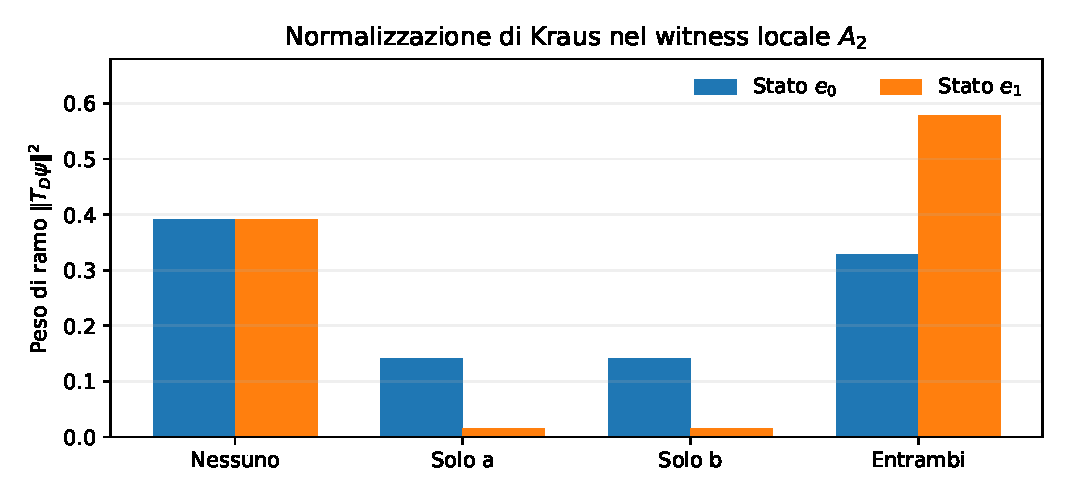
\includegraphics[width=0.66\linewidth]{R12BB_ON_BRANCH_WEIGHTS.pdf}
\caption{Pesi dei quattro rami del solo genitore $A_2$ in due stati interni. La somma vale uno in entrambe le colonne; la figura non dimostra general covariance o causalita quantistica di Bell.}
\end{figure}
\textbf{Controllo negativo:} il kernel banale $T_D=I/4$ soddisfa la prima somma, ma $\sum_D T_D^\dagger T_D=I/4$, non $I$. Le due condizioni non devono essere trattate come sinonimi.

\textbf{Audit indipendente.} SymPy e un motore separato con \texttt{fractions.Fraction} su $\mathbb Q(\sqrt{21})$ restituiscono \textbf{ledger byte-identici} per matrici, determinanti, commutatori, Gram e interferenza. Il testimone e esplorativo, il freeze precede la verifica indipendente; un errore tecnico di indicizzazione vettoriale e documentato nel QA.

\textbf{Limiti.} La simmetria $a\leftrightarrow b$ del genitore $A_2$ \emph{non} prova covarianza globale. Non sono state verificate le relazioni complete di \emph{quantum Bell causality} (QBC) operatoriale, ne alcuna estensione a tutti i genitori. La completezza di Kraus e un'ipotesi addizionale; l'azione BDG \emph{non entra} nel witness. Nessuna misura gravitazionale, geometria dinamica 4D, identita Bianchi/Ward o legge $H(z)$ e derivata.

\textbf{Decisione R12bb-ON:} compatibilita locale di due normalizzazioni e noncommutativita \textbf{PASS}; \textbf{QBC completa NON DERIVATA}. \textbf{R12bc NON APERTO, R12as fisico NON AUTORIZZATO, R13 BLOCCATO.}

\textbf{Fonti.} \href{https://doi.org/10.1103/thx5-dknv}{Srivastava--Surya, Phys. Rev. D 114, 086007 (2026)} (QBC noncommutativa); \href{https://eu-de.quantum.cloud.ibm.com/learning/en/courses/general-formulation-of-quantum-information/quantum-channels/representations-of-channels}{IBM Quantum Learning, Kraus representations} (completezza di canale). Il risultato e un controllo matematico locale, non una nuova teoria fisica.

\clearpage
\section*{Appendice R12bb-RB --- Ostruzione al collegamento della prima nascita (v0.87)}
\textbf{Motivazione.} La v0.86 aveva costruito un testimone esatto non commutativo di quattro transizioni dal solo genitore anticatena $A_2$, con la somma operatoriale delle ampiezze e la completezza di Kraus simultaneamente valide. Il risultato non conteneva ancora una regola per la prima nascita. Verifichiamo ora \emph{senza cambiare il testimone} una relazione necessaria della \emph{causal-past-ordered quantum Bell causality} (CPOBC) di Srivastava--Surya. La completezza di Kraus resta una \textbf{ipotesi diagnostica aggiuntiva}, non un assioma dimostrato della crescita quantistica.

\subsection*{RB.1 --- Relazione causale necessaria e soluzione unica}
Sia $G_1$ il ramo di nascita senza precursori dal singoletto e $B_1$ il ramo con il singoletto nel passato. La somma delle ampiezze impone $G_1+B_1=I$. Sul genitore $A_2$ fissiamo gli operatori della v0.86:
\begin{equation}
 G_2=\frac14I+\frac{\sqrt{21}}8X,\qquad
 B_2=\frac14I+\frac18Z,\quad
 X=\begin{pmatrix}0&1\\1&0\end{pmatrix},\quad Z=\operatorname{diag}(1,-1).\tag{RB.1}
\end{equation}
Qui $G_2$ e il ramo vuoto e $B_2$ e ciascuno dei due rami di precursore singoletto. La relazione CPOBC per le coppie di Bell collegate, nell'ordinamento di \href{https://arxiv.org/html/2603.25503}{Srivastava--Surya, Eq.~(107)}, richiede, assumendo $G_1$ invertibile,
\begin{equation}
 B_2=B_1G_2G_1^{-1},\qquad
 \boxed{B_2G_1+G_1G_2=G_2}.\tag{RB.2}
\end{equation}
\textbf{Questo e un vincolo necessario sotto CPOBC, non l'intera condizione globale.} Scrivendo $G_1=\left(\begin{smallmatrix}a&b\\c&d\end{smallmatrix}\right)$, il sistema lineare per $(a,b,c,d)$ ha matrice dei coefficienti
\begin{equation}
 M=\begin{pmatrix}
 5/8&\sqrt{21}/8&0&0\\
 \sqrt{21}/8&5/8&0&0\\
 0&0&3/8&\sqrt{21}/8\\
 0&0&\sqrt{21}/8&3/8
 \end{pmatrix},\qquad
 \boxed{\det M=-\frac3{256}\ne0}.\tag{RB.3}
\end{equation}
La soluzione e pertanto \emph{unica} e si verifica per sostituzione esatta:
\begin{equation}
 \boxed{G_1=\begin{pmatrix}-11/4&3\sqrt{21}/4\\-\sqrt{21}/12&5/4\end{pmatrix}}.\tag{RB.4}
\end{equation}

\clearpage
\subsection*{RB.2 --- Incompatibilita con Kraus gia alla radice}
Imporre anche la completezza di Kraus al genitore singoletto richiederebbe
\begin{equation}
 G_1^\dagger G_1+(I-G_1)^\dagger(I-G_1)=I
 \quad\Longrightarrow\quad G_1^\dagger G_1\le I.\tag{RB.5}
\end{equation}
Ogni elemento di matrice di una contrazione ha modulo al piu uno. Ma dalla (RB.4) si trova immediatamente
\begin{equation}
 \boxed{|(G_1)_{11}|=\frac{11}{4}>1},\qquad
 G_1^\dagger G_1+(I-G_1)^\dagger(I-G_1)-I
 =\begin{pmatrix}251/12&-5\sqrt{21}\\-5\sqrt{21}&97/4\end{pmatrix}\ne0.\tag{RB.6}
\end{equation}
La traccia del residuo e $271/6$, diversa da zero. In definitiva, il \textbf{testimone NON commutativo specifico di v0.86 non ammette una prima biforcazione} che conservi simultaneamente la relazione (RB.2), il MSR $G_1+B_1=I$ e l'ipotesi aggiuntiva di Kraus. Le normalizzazioni locali gia dimostrate per $A_2$ \emph{non vengono invalidate}: il problema nasce nel collegarle al genitore precedente.

\subsection*{RB.3 --- Controllo positivo esatto, senza selezione fisica}
Una famiglia scalare commutativa mostra che il controllo non e una contraddizione dell'algebra usata. Consideriamo i seguenti operatori, tutti multipli non nulli dell'identita:
\begin{equation}
 \begin{aligned}
 G_1&=\tfrac{1-i}2I,&B_1&=\tfrac{1+i}2I,\\
 G_2&=\tfrac14I,&B_{2,a}=B_{2,b}&=\tfrac{i}4I,\\
 &&T_{2,ab}&=(\tfrac34-\tfrac i2)I.
 \end{aligned}\tag{RB.7}
\end{equation}
Allora le due somme $G_1+B_1=I$ e $G_2+B_{2,a}+B_{2,b}+T_{2,ab}=I$, le due somme di Kraus, e la stessa relazione di Bell $B_{2,a}G_1=B_1G_2=(1+i)I/8$ risultano \textbf{esattamente vere}. Non e stata affermata una realizzazione globale, ma la contraddizione specifica del witness non e un difetto logico delle condizioni.

\textbf{Audit.} Dopo la scoperta esplorativa, il protocollo e stato congelato prima del controllo indipendente. SymPy e un secondo solutore 4\,$\times$\,4 scritto con \texttt{fractions.Fraction} su $\mathbb Q(\sqrt{21})$ riproducono lo \textbf{stesso registro JSON byte per byte}; il controllo positivo e verificato con razionali gaussiani esatti. \textbf{Limiti:} nessun no-go per tutte le rappresentazioni non commutative o per QSG senza Kraus, nessuna CPOBC completa, nessuna misura BDG fisicamente selezionata, nessuna gravitazione dinamica 4D e nessuna legge $H(z)$. \textbf{R12bc NON APERTO; R12as fisico NON AUTORIZZATO; R13 BLOCCATO.}

\clearpage
\section*{Appendice R12bb-NK --- Vincolo CPOBC senza Kraus (v0.88)}
\textbf{Domanda.} Nella v0.87 il testimone operatoriale non commutativo di v0.86 risultava incompatibile con una \emph{ulteriore} normalizzazione di Kraus alla prima nascita. Questa appendice rimuove \emph{completamente} Kraus dalle ipotesi. Lasciamo \textbf{immutati} tutti gli operatori del genitore anticatena $A_2$ e verifichiamo una successiva relazione necessaria della causal-past-ordered quantum Bell causality (CPOBC) non singolare. Il risultato e una \textbf{ostruzione per questo solo testimone}, non una classificazione delle rappresentazioni non commutative.

\subsection*{NK.1 --- Il collegamento iniziale riesce senza Kraus}
Siano $I$ l'identita $2\times2$, $X=\left(\begin{smallmatrix}0&1\\1&0\end{smallmatrix}\right)$ e $Z=\operatorname{diag}(1,-1)$. Manteniamo i generatori del testimone storico:
\begin{equation}
Q_2=G_2=\frac14 I+\frac{\sqrt{21}}8X,\qquad B_2=\frac14 I+\frac18 Z.
\tag{NK.1}
\end{equation}
Il MSR al singoletto impone $G_1+B_1=I$. La relazione CPOBC necessaria \href{https://arxiv.org/html/2603.25503}{Srivastava--Surya, Eq.~(107)} richiede $B_2G_1=B_1G_2$. Risolvendo il sistema lineare su $\mathbb Q(\sqrt{21})$ si ottengono \emph{univocamente}
\begin{equation}
\begin{aligned}
Q_1=G_1&=\begin{pmatrix}-11/4&3\sqrt{21}/4\\-\sqrt{21}/12&5/4\end{pmatrix},\\
B_1=I-G_1&=\begin{pmatrix}15/4&-3\sqrt{21}/4\\\sqrt{21}/12&-1/4\end{pmatrix},\\
\det G_1&=-17/8,\qquad \det B_1=3/8.
\end{aligned}\tag{NK.2}
\end{equation}
Poiche entrambi i determinanti sono non nulli, l'ostacolo \emph{non} e l'invertibilita della radice. Il primo diamante di covarianza e compatibile: il ramo gregarious dal genitore catena $K_2$ puo essere definito senza parametri nuovi da
\begin{equation}
G_{K_2}=B_1Q_2B_1^{-1}
=\begin{pmatrix}-5/8&3\sqrt{21}/4\\-\sqrt{21}/36&9/8\end{pmatrix},\qquad
G_{K_2}B_1=B_2G_1.
\tag{NK.3}
\end{equation}
Anche gli altri due rami del genitore catena possono essere completati localmente senza parametri nuovi: $B_{K_2}=B_1G_{K_2}G_1^{-1}$ e $T_{K_2}=I-G_{K_2}-B_{K_2}$. Per essi, e per il ramo vuoto, risulta
\begin{equation}
\det G_{K_2}=-\frac{17}{64},\qquad \det B_{K_2}=\frac3{64},\qquad
\det T_{K_2}=-\frac3{32}.\tag{NK.3a}
\end{equation}
Si ha quindi una prima estensione locale con MSR e rami non singolari, oltre al diamante di covarianza verificato; questo \emph{non} garantisce le relazioni globali successive. Le somme di ampiezza al singoletto e ad $A_2$ restano uguali a $I$. \textbf{Nessuna condizione di Kraus e imposta in questo audit}; il suo precedente FAIL resta soltanto un dato storico.

\clearpage
\subsection*{NK.2 --- Fallimento del vincolo necessario tra generatori}
Per una crescita \emph{globale} non singolare che soddisfi l'intera CPOBC, \href{https://arxiv.org/html/2603.25503}{Srivastava--Surya, Corollary 3.9, Eq.~(130)} forniscono la condizione necessaria
\begin{equation}
\boxed{\bigl[Q_1Q_2^{-1},\ Q_1^{-1}Q_2\bigr]=0},\qquad Q_1=G_1,\quad Q_2=G_2.\tag{NK.4}
\end{equation}
Sostituendo \emph{senza variare} (NK.1)--(NK.2), il commutatore esatto e
\begin{equation}
\boxed{
\bigl[Q_1Q_2^{-1},\ Q_1^{-1}Q_2\bigr]
=\begin{pmatrix}
-112/17&22\sqrt{21}/17\\
-74\sqrt{21}/51&112/17
\end{pmatrix}},\quad
\boxed{\det=-\frac{1148}{289}\ne0}.\tag{NK.5}
\end{equation}
In particolare la matrice non e nulla (la traccia vale zero). La (NK.4) e \textbf{violata}: \emph{il testimone fisso di v0.86 non puo essere prolungato a una crescita operatoriale globale non singolare che soddisfi la CPOBC completa, anche rinunciando a Kraus}. Il primo diamante che funziona non basta per la consistenza delle generazioni successive.

\subsection*{NK.3 --- Controlli, limiti e decisione}
\textbf{Controllo positivo.} Per $Q_1=I/2$, $Q_2=I/4$ (percolazione scalare $p=1/2$), la relazione (NK.4) e identicamente nulla e il legame iniziale $B_2G_1=B_1G_2$, con $B_1=I/2$ e $B_2=I/4$, e esatto. Questo conferma che il test necessario non e di per se contraddittorio; non implica che tutte le matrici ammissibili debbano commutare.

\textbf{Audit indipendente.} Un primo programma SymPy risolve il sistema di Sylvester ed esegue il test della (NK.4). Un secondo programma, sviluppato separatamente con \texttt{fractions.Fraction} e un campo quadratico esatto $\mathbb Q(\sqrt{21})$, riproduce \textbf{lo stesso registro JSON byte per byte}. I controlli includono gli otto determinanti non nulli dei rami nel primo tratto della crescita, il primo diamante di covarianza e il test positivo scalare. Il protocollo e stato congelato dopo la scoperta esplorativa e prima della validazione indipendente: non e rivendicata una previsione preregistrata.

\textbf{Confini della conclusione.} La (NK.5) riguarda esclusivamente il \emph{witness preesistente} e non esclude altre rappresentazioni $2\times2$, dimensioni maggiori o tutte le misure quantistiche di crescita. Non sono costruiti operatori globali alternativi, non si incorpora l'azione BDG nelle nuove transizioni, non si deriva gravita dinamica 4D, conservazione Ward/Bianchi o $H(z)$. \textbf{Decisione R12bb-NK: FAIL globale necessario per il witness fisso, PASS come audit esatto. R12bc NON APERTO; R12as fisico NON AUTORIZZATO; R13 BLOCCATO.}

\clearpage
\section*{Appendice v0.89 --- R12bb-NC: generatori normali $2\times2$ e vincolo CPOBC}
\addcontentsline{toc}{section}{Appendice v0.89 --- R12bb-NC}
\textbf{Ambito e fonte.} La relazione seguente e una condizione \emph{necessaria}, non sufficiente, per una crescita quantistica operatoriale non singolare con Bell causality ordinata secondo il passato (Srivastava--Surya, \emph{Phys. Rev. D} \textbf{114}, 086007, 2026, Corollario 3.9, Eq. 130):
\begin{equation}
[Q_1Q_2^{-1},\,Q_1^{-1}Q_2]=0. \tag{NC.1}
\end{equation}
Qui esaminiamo l'intera classe delle coppie \emph{normali e invertibili} $2\times2$, senza fissare nuove matrici di transizione, senza imporre Kraus e senza aprire un gate gravitazionale.

\subsection*{NC.1 --- Teorema di classificazione (settore normale)}
\textbf{Teorema.} Siano $A,B\in M_2(\mathbb C)$ normali e invertibili. Allora
\begin{equation}
[AB^{-1},A^{-1}B]=0\quad\Longleftrightarrow\quad
[A,B]=0\ \ \text{oppure}\ \ \operatorname{tr}A=\operatorname{tr}B=0.\tag{NC.2}
\end{equation}
\textbf{Dimostrazione.} Tramite una coniugazione unitaria comune (che lascia invariata la condizione) diagonalizziamo $A$:
\begin{equation}
A=\begin{pmatrix}a&0\\0&b\end{pmatrix},\qquad
B=\begin{pmatrix}c&u\\v&d\end{pmatrix},\qquad
ab(cd-uv)\ne0.\tag{NC.3}
\end{equation}
Con $\Delta=ab(cd-uv)$, l'espansione diretta degli inversi da la seguente identita \emph{polinomiale esatta}:
\begin{equation}
\Delta[AB^{-1},A^{-1}B]=
\begin{pmatrix}
-uv(a-b)(a+b)&-u(a-b)(ad-bc)\\
-v(a-b)(ad-bc)&uv(a-b)(a+b)
\end{pmatrix}.\tag{NC.4}
\end{equation}
Se $[A,B]\ne0$, allora $a\ne b$ e almeno uno fra $u,v$ e non nullo. Poiche $B$ e normale, $|u|=|v|$: entrambi sono non nulli. L'annullamento della voce diagonale di (NC.4) forza $a+b=0$; l'annullamento della voce fuori diagonale forza $ad-bc=a(d+c)=0$, dunque $c+d=0$. Sono nulle le tracce di entrambi i generatori.

Viceversa, se $\operatorname{tr}A=\operatorname{tr}B=0$, Cayley--Hamilton da $A^2=-\det(A)I$ e $B^2=-\det(B)I$. Pertanto $AB^{-1}$ e $A^{-1}B$ sono multipli scalari della stessa matrice $AB$ e commutano. Se $[A,B]=0$, anche gli inversi commutano. Questo conclude la dimostrazione.

\newpage
\newpage
\subsection*{NC.2 --- Implicazioni e controcontrolli}
\textbf{Corollario positivo.} Per $A,B$ hermitiane definite positive $2\times2$, la (NC.1) implica $[A,B]=0$: la possibilita a tracce nulle non e disponibile. Piu in generale, in questa classe normale, una coppia noncommutativa che passa (NC.1) deve avere entrambe le tracce nulle. L'ipotesi di normalita resta \textbf{aggiuntiva}, non una legge microfisica derivata.

L'esempio positivo-definito non commutativo $A=\operatorname{diag}(1/4,1/2)$, $B=\left(\begin{smallmatrix}1/3&1/10\\1/10&1/3\end{smallmatrix}\right)$ da un residuo non nullo:
\begin{equation}
[AB^{-1},A^{-1}B]=
\begin{pmatrix}27/182&-15/91\\-15/91&-27/182\end{pmatrix}\ne0.\tag{NC.5}
\end{equation}
Per contro, $A=\operatorname{diag}(1/2,-1/2)$ e $B=\left(\begin{smallmatrix}1/3&1/5\\1/5&-1/3\end{smallmatrix}\right)$ sono hermitiane, non commutano, hanno traccia nulla e soddisfano esattamente (NC.1). Quindi la (NC.1) \emph{non} forza commutativita senza ipotesi ulteriori.

\textbf{Limite indispensabile.} Sostituire ``normale'' con ``spettro positivo'' invaliderebbe l'enunciato. Con $A=\operatorname{diag}(1/4,1/2)$ e $B=\left(\begin{smallmatrix}1/4&1/8\\0&1/2\end{smallmatrix}\right)$, entrambe hanno autovalori positivi e $[A,B]\ne0$, ma $B$ non e normale e (NC.1) e soddisfatta. L'esistenza di questo controesempio impedisce un no-go piu ampio.

\subsection*{NC.3 --- Audit esatto e decisione}
La prima verifica espande simbolicamente l'intera matrice (NC.4) in sei indeterminate con SymPy. La seconda realizza \emph{indipendentemente}, senza SymPy, un anello polinomiale intero e un motore su gaussiani razionali; le quattro componenti del numeratore e cinque controlli esatti coincidono nei registri JSON \textbf{byte per byte} (SHA-256 integrale conservato nel protocollo e nei ledger). Scoperta esplorativa precedente al congelamento del protocollo; nessuna pretesa di discovery preregistrata.

\textbf{Confini.} La normalita e una scelta di sottosettore, non deriva dalla CPOBC. Non sono verificate le relazioni successive (come Eq. 145), la consistenza globale o il limite 4D; ne viene incorporata l'azione BDG nei generatori. Il risultato e una \emph{classificazione necessaria condizionata}, non una misura fisica o una soluzione QSG. \textbf{R12bc NON APERTO; R12as fisico NON AUTORIZZATO; R13 BLOCCATO.}


\clearpage
\section*{Appendice v0.90 --- R12bb-PL: rigidita dei generatori CPOBC}
\addtocontents{toc}{\protect\enlargethispage{5\baselineskip}}
\addcontentsline{toc}{section}{Appendice v0.90 --- R12bb-PL}
\textbf{Autorita e ambito.} Srivastava e Surya, \emph{Phys. Rev. D} \textbf{114}, 086007 (2026), derivano per una crescita CPOBC non singolare le relazioni \emph{necessarie} (119), (128) e (130). La v0.89 ha classificato la (130) nella classe delle coppie normali invertibili $2\times2$. Qui usiamo anche la (119), senza ipotizzare che tali relazioni siano sufficienti o che la normalita sia un assioma fisico.

\subsection*{PL.1 --- Teorema di rigidita lineare}
\textbf{Teorema.} Siano $Q_1,Q_2\in M_2(\mathbb C)$ normali, invertibili e non commutanti, con
\begin{equation}
[Q_1Q_2^{-1},Q_1^{-1}Q_2]=0.\tag{PL.1}
\end{equation}
Se per ogni $n\ge3$ un generatore invertibile $Q_n$ soddisfa la relazione CPOBC necessaria (119) per $k=1,m=2$,
\begin{equation}
Q_nQ_1^{-1}Q_2=Q_2Q_1^{-1}Q_n,\tag{PL.2}
\end{equation}
allora
\begin{equation}
\boxed{\quad Q_n=\alpha_nQ_1+\beta_nQ_2,\qquad
\operatorname{tr}(Q_n)=0\quad(n\ge3).\quad}\tag{PL.3}
\end{equation}
\textbf{Dimostrazione.} Per la classificazione v0.89, la (PL.1) e la noncommutativita implicano $\operatorname{tr}Q_1=\operatorname{tr}Q_2=0$. Mediante una base ortonormale diagonalizziamo il primo generatore:
\begin{equation}
Q_1=\begin{pmatrix}a&0\\0&-a\end{pmatrix},\quad
Q_2=\begin{pmatrix}c&u\\v&-c\end{pmatrix},\quad
Q_n=\begin{pmatrix}x&y\\z&w\end{pmatrix},\quad a\ne0.\tag{PL.4}
\end{equation}
La normalita di $Q_2$ implica $|u|=|v|$; poiche $[Q_1,Q_2]\ne0$, risulta $uv\ne0$. L'espansione senza approssimazioni da
\begin{equation}
 a\left(Q_nQ_1^{-1}Q_2-Q_2Q_1^{-1}Q_n\right)
 =\begin{pmatrix}uz-vy&u(x+w)\\-v(x+w)&uz-vy\end{pmatrix}.\tag{PL.5}
\end{equation}
Pertanto $w=-x$ e $uz=vy$. Basta porre $\beta_n=y/u=z/v$ e $\alpha_n=(x-\beta_nc)/a$. Si ottiene esattamente la (PL.3). \emph{Non} e stata assunta la normalita di $Q_n$ per $n\ge3$. L'invertibilita richiede unicamente $\det Q_n\ne0$.

\clearpage
\subsection*{PL.2 --- Le altre identita necessarie non selezionano i coefficienti}
Scriviamo $A=Q_1$, $B=Q_2$ e $Q_j=\alpha_j A+\beta_jB$. Poiche $A$ e $B$ sono traceless e invertibili, Cayley--Hamilton implica
\begin{equation}
 A^2=\kappa I,\quad B^2=\lambda I,\quad AB+BA=\tau I,\qquad
 \kappa,\lambda\ne0.\tag{PL.6}
\end{equation}
Anche $Q_j^{-1}$ e multiplo di $Q_j$. In particolare ogni prodotto $Q_i^{-1}Q_j$ appartiene allo spazio commutativo
\begin{equation}
 \operatorname{span}_{\mathbb C}\{I,AB\};\qquad
 [Q_i^{-1}Q_j,Q_k^{-1}Q_\ell]=0.\tag{PL.7}
\end{equation}
La relazione necessaria (128) segue, mentre la (119) segue dalla trilinearita di $XYZ-ZYX$: per ogni tripla di fattori scelta nello spazio $\operatorname{span}\{A,B\}$, ogni termine base con un generatore ripetuto si annulla per la (PL.6). Anche la (130) e soddisfatta. Questi vincoli \emph{da soli} lasciano libere infinite scelte invertibili dei coefficienti $(\alpha_j,\beta_j)$.

\subsection*{PL.3 --- Controlli esatti, esempi e limiti}
Per verificare, senza \emph{fit}, le sole identita necessarie si utilizzano matrici diagnostiche normali, invertibili e a traccia nulla:
\begin{equation}
\begin{split}
Q_1&=\begin{pmatrix}1&0\\0&-1\end{pmatrix},\quad
Q_2=\begin{pmatrix}0&1\\1&0\end{pmatrix},\quad
Q_3=\begin{pmatrix}2&3\\3&-2\end{pmatrix},\\
Q_4&=\begin{pmatrix}1&-2\\-2&-1\end{pmatrix},\quad
Q_5=\begin{pmatrix}2&1\\1&-2\end{pmatrix}.
\end{split}\tag{PL.8}
\end{equation}
Due implementazioni autonome (SymPy e anello polinomiale/frazioni senza SymPy) concordano \emph{byte per byte}: 10 controlli Eq.~(119), 120 commutatori Eq.~(128), Eq.~(130) e due controlli negativi che inseriscono una componente fuori piano. Sono verifiche algebriche, \textbf{non} transizioni di un modello QSG completo.

\textbf{Limite di interpretazione.} La (PL.3) e un teorema \emph{condizionato}: la normalita dei primi due generatori non e stata derivata, la (119) e la (128) sono necessarie ma non sufficienti, e non sono risolte le ulteriori condizioni CPOBC (come le Eq.~139 e 145), la covarianza globale o la selezione della misura. Nessuna azione BDG e stata incorporata nei generatori. Non sono derivate gravita dinamica 4D, conservazione gravitazionale o una legge $H(z)$.

\textbf{Decisione:} \textsf{R12bb-PL PASS matematico condizionato. R12bc NON APERTO; R12as fisico NON AUTORIZZATO; R13 BLOCCATO.}

\clearpage
\section*{Appendice v0.91 --- R12bb-E2: condizione CPOBC di livello due}
\addcontentsline{toc}{section}{Appendice v0.91 --- R12bb-E2}
\textbf{Premesse e autorita.} La v0.90 ha imposto, in una sottoclasse normale non commutativa $2\times2$, la forma $Q_3=\alpha Q_1+\beta Q_2$ tramite relazioni \emph{necessarie} sulle anticatene. Qui si aggiunge una diversa condizione necessaria della CPOBC non singolare, ottenuta da Srivastava--Surya (arXiv:2603.25503, Eqs. 139 e 145), che collega i primi operatori di transizione effettivi. \textbf{Non} si tratta di una verifica della CPOBC completa.

\subsection*{E2.1 --- Condizione necessaria pubblicata}
Posti $A=Q_1$, $B=Q_2$, $C=Q_3$, definiamo
\begin{equation}
 P=(I-A)BA^{-1},\qquad T=I-2P-B.\tag{E2.1}
\end{equation}
Essi rappresentano le transizioni con uno o due precursori dall'anticatena $a_2$. La condizione (139), nella specializzazione esplicita (145), impone
\begin{equation}
 PTCT^{-1}B^{-1}T=TP CP^{-1}B^{-1}P.\tag{E2.2}
\end{equation}
Tutte le inversioni richieste devono esistere.

\subsection*{E2.2 --- Coppia storica e certificato esatto}
Conserviamo \emph{senza alcuna modifica} la coppia normale non commutativa gia presente nella v0.89:
\begin{equation}
 A=\begin{pmatrix}\tfrac12&0\\0&-\tfrac12\end{pmatrix},\qquad
 B=\begin{pmatrix}\tfrac13&\tfrac15\\\tfrac15&-\tfrac13\end{pmatrix},\qquad
 [A,B]=\begin{pmatrix}0&\tfrac15\\-\tfrac15&0\end{pmatrix}.\tag{E2.3}
\end{equation}
Ambedue sono hermitiane, invertibili e a traccia nulla: superano la necessaria Eq. 130. Le matrici in (E2.1) sono
\begin{equation}
 P=\begin{pmatrix}\tfrac13&-\tfrac15\\\tfrac35&1\end{pmatrix},\quad
 T=\begin{pmatrix}0&\tfrac15\\-\tfrac75&-\tfrac23\end{pmatrix};\qquad
 \det P=\tfrac{34}{75},\quad\det T=\tfrac7{25}.\tag{E2.4}
\end{equation}
Anche $\det A=-1/4$, $\det(I-A)=3/4$, $\det B=-34/225$ sono non nulli; gli operatori ricostruiti dal ramo a catena al secondo stadio sono invertibili nel controllo.

Scriviamo $\mathcal D(C)$ per \emph{primo membro meno secondo membro} della (E2.2). Essendo $\mathcal D$ lineare, $\mathcal D(C)=\alpha\mathcal D(A)+\beta\mathcal D(B)$. Le sole voci $(1,2)$ e $(2,1)$ impongono
\begin{equation}
 \underbrace{\begin{pmatrix}-\tfrac{45}{289}&-\tfrac{1998}{10115}\\-\tfrac{655}{289}&\tfrac{2642}{4335}\end{pmatrix}}_{M}
 \begin{pmatrix}\alpha\\\beta\end{pmatrix}=0,\qquad
 \boxed{\det M=-\frac{18660}{34391}\ne0}.\tag{E2.5}
\end{equation}
Quindi $\alpha=\beta=0$, percio $Q_3=0$ e non e invertibile. \textbf{Teorema ristretto:} la coppia fissa (E2.3), pur compatibile con i vincoli sulle anticatene, non ammette prosecuzione non singolare che soddisfi anche la (E2.2).

\clearpage
\subsection*{E2.3 --- Corollario generico e limiti}
Ogni coppia hermitiana traceless non commutativa $2\times2$ e, per coniugazione unitaria, rappresentabile come
\begin{equation}
 A=a\sigma_z,\qquad B=b\sigma_z+u\sigma_x,\qquad a,b,u\in\mathbb R,\quad au\ne0.\tag{E2.6}
\end{equation}
Sul dominio in cui esistono gli inversi richiesti, le entrate di $\mathcal D(A),\mathcal D(B)$ e il minor (E2.5) sono funzioni \emph{razionali} di $(a,b,u)$. Il valore esatto non nullo alla coppia storica prova che il minor non e identicamente zero. Pertanto esso resta non nullo su un \emph{insieme aperto e denso} della famiglia hermitiana ammissibile; qui la (E2.2) esclude ogni $Q_3$ invertibile nello span.

\textbf{Non e un no-go universale.} L'insieme eccezionale dove il minor si annulla non e stato classificato; altre rappresentazioni normali non hermitiane, non normali oppure di dimensione maggiore non vengono escluse. La normalita dei generatori non e stata giustificata fisicamente. In particolare non sono derivati misura quantistica delle geometrie, teoria gravitazionale 4D, Ward on-shell, risposta retarded o una predizione autonoma $H(z)$.

\textbf{Audit.} Il motore SymPy implementa la Eq. 145 in forma espansa; un secondo motore con sole frazioni razionali implementa la Eq. 139 compatta. Entrambi verificano il minor, le invertibilita iniziali e un controllo commuting, restituendo risultati JSON identici byte per byte. La scoperta e \emph{esplorativa}, non preregistrata: il protocollo e stato consolidato prima del replay finale, dopo la prima verifica dei calcoli.

\textbf{Decisione:} \textsf{R12bb-E2 PASS matematico di ostruzione condizionata; CPOBC globale NON risolta; R12bc NON APERTO; R12as fisico NON AUTORIZZATO; R13 BLOCCATO.}

\clearpage
\begingroup
\setlength{\parskip}{0.16em}
\section*{Appendice v0.92 --- R12bb-XL: classificazione del locus eccezionale}
\addcontentsline{toc}{section}{Appendice v0.92 --- R12bb-XL}
\textbf{Oggetto.} La v0.91 ha escluso una coppia storica hermitiana $2\times2$ tramite la relazione necessaria (139)/(145) di Srivastava--Surya. Il suo corollario aperto--denso lasciava irrisolti i casi eccezionali. Qui li classifichiamo \emph{simbolicamente in tutto il settore hermitiano, invertibile, traceless e non commutativo} a livello delle condizioni necessarie (119), (130) e (145). La fonte delle identita CPOBC e Srivastava--Surya (2026), Sez.~3.5; la classificazione parametrica e un risultato interno condizionato.

\subsection*{XL.1 --- Teorema di classificazione locale}
Sia $Q_1,Q_2$ una coppia hermitiana invertibile $2\times2$ con traccia nulla e $[Q_1,Q_2]\ne0$. Una coniugazione unitaria comune, usando anche il riaggiustamento della fase fuori diagonale, porta senza perdita di generalita a
\begin{equation}
 A=Q_1=\begin{pmatrix}a&0\\0&-a\end{pmatrix},\quad
 B=Q_2=\begin{pmatrix}b&u\\u&-b\end{pmatrix},\qquad
 a,b,u\in\mathbb R,\quad au\ne0.\tag{XL.1}
\end{equation}
Il teorema v0.90, usando la (119), impone a ogni eventuale terzo generatore non singolare la forma $C=Q_3=\alpha A+\beta B$, con $\alpha,\beta\in\mathbb C$. Dalle transizioni di secondo stadio si hanno
\begin{equation}
 P=(I-A)BA^{-1},\quad T=I-2P-B,\quad
 PTCT^{-1}B^{-1}T=TP CP^{-1}B^{-1}P.\tag{XL.2}
\end{equation}
Richiediamo invertibili $A,I-A,B,P,T,C$ e gli altri operatori ricostruiti a questo livello.

\textbf{Teorema (esattamente per il gate locale).} La (XL.2), insieme alle condizioni (119) e (130), ammette $C$ non nullo e invertibile nel suddetto dominio hermitiano non commutativo \emph{se e soltanto se}
\begin{equation}
 \boxed{\quad b=-\frac{1}{4a},\qquad u^2=\frac{4a^2-1}{16a^2},\qquad
 C=\beta B,\quad\beta\in\mathbb C\setminus\{0\}\quad}\tag{XL.3}
\end{equation}
con $|a|>1/2$, $a^2\ne1,2$ e con l'uno o l'altro segno reale di $u$. Non e un teorema di esistenza di una CPOBC globale.

\subsection*{XL.2 --- La similitudine impone il primo vincolo}
Siano $K=P^{-1}T^{-1}PT$ e $W=P^{-1}B^{-1}PT^{-1}BT$. La (XL.2) equivale a $KC=CW$; $C$ invertibile rende $K$ e $W$ simili, quindi ne impone l'uguaglianza delle tracce. Ponendo $s=b^2+u^2$ e $F=a^2b^2+9a^2u^2-a^2+4ab-4s$, il calcolo esatto fornisce
\begin{equation}
 \operatorname{tr}(K)-\operatorname{tr}(W)=
 \frac{4a^2u^2(s-4a^2b^2)}{(a^2-1)s^2F}.\tag{XL.4}
\end{equation}
Poiche i denominatori sono non nulli dove la (XL.2) e definita, e $au\ne0$, si ottiene la relazione necessaria
\begin{equation}
 u^2=(4a^2-1)b^2.\tag{XL.5}
\end{equation}
La realta e $u\ne0$ obbligano $b\ne0$ e $|a|>1/2$; la coppia storica v0.91 viola gia questo vincolo (gap di traccia esatto $2700/2023$).

\clearpage
\subsection*{XL.3 --- Il minor di rango e la sufficienza esatta}
Sulla superficie (XL.5) poniamo $J=6a^2b+a-4b$. La non singolarita di $T$ impone $(6ab-1)J\ne0$, poiche $\det T=-(6ab-1)J/a$. Definiamo
\begin{equation}
 E_A=KA-AW,\qquad E_B=KB-BW,\qquad\alpha E_A+\beta E_B=0.\tag{XL.6}
\end{equation}
Le loro componenti diagonali soddisfano le identita esatte
\begin{align}
 (E_A)_{11}=(E_A)_{22}&=\frac{a(4a^2-1)}{2(a^2-1)J},\notag\\
 (E_B)_{11}=-(E_B)_{22}&=-\frac{ab(4a^2-1)(4ab+1)}{(a^2-1)J}.\tag{XL.7}
\end{align}
Il minor corrispondente dei due vincoli lineari su $(\alpha,\beta)$ e
\begin{equation}
 \boxed{\;\Delta_{\mathrm{diag}}=
 \frac{a^2b(4a^2-1)^2(4ab+1)}{(a^2-1)^2J^2}.\;}\tag{XL.8}
\end{equation}
Nel dominio considerato tutti i fattori, eccetto l'ultimo nel numeratore, sono non nulli: $4ab+1=0$ e dunque necessario. Sostituendolo nella (XL.5) si ottengono esattamente i primi due vincoli (XL.3), con
\begin{equation}
 B^2=\frac14 I,\qquad AB+BA=-\frac12 I,\qquad
 E_B=0,\quad E_A=-\frac{a^2(4a^2-1)}{(a^2-1)(a^2-2)}I.\tag{XL.9}
\end{equation}
La terza identita matriciale e verificata in \emph{tutte} le entrate: $C=\beta B$ soddisfa la Eq.~145. La quarta mostra che nessuna componente $\alpha A$ puo sopravvivere. Con $\beta\ne0$ si ha $\det C=-\beta^2/4\ne0$.

Gli operatori di livello due, definiti come in Srivastava--Surya, non vengono resi artificialmente singolari:
\begin{equation}
\begin{gathered}
\det A=-a^2,\quad \det(I-A)=1-a^2,\quad \det B=-\tfrac14,\\
\det P=\det V=\frac{1-a^2}{4a^2},\quad
\det T=\frac{5(2-a^2)}{4a^2},\quad
\det G=-\tfrac14,\quad\det T^{\mathrm{chain}}=\frac1{a^2}.\tag{XL.10}
\end{gathered}
\end{equation}
Questi determinanti spiegano le sole esclusioni $a^2=1,2$ oltre al bordo $|a|=1/2$ (che toglierebbe la noncommutativita). Non e stata scelta alcuna matrice cercando di far passare il test: l'intera curva deriva dal sistema simbolico.

\subsection*{XL.4 --- Certificati e limiti scientifici}
Il motore \texttt{R12BB\_XL\_PRIMARY.py} usa SymPy con inversi razionali simbolici. Il secondo motore \texttt{R12BB\_XL\_INDEPENDENT.py} implementa \emph{senza SymPy} un anello di polinomi multivariati a coefficienti interi, usando aggiunte e prodotti di matrici adjugate; per i numeratori $K_{\rm num},W_{\rm num}$ dimostra coefficient-by-coefficient
\begin{equation}
 \operatorname{tr}(K_{\rm num}-W_{\rm num})=4a^2u^2(s-4a^2b^2).\tag{XL.11}
\end{equation}
La riduzione del minor numeratore modulo (XL.5) da esattamente
\begin{equation}
 256a^{12}b^9(4a^2-1)^2(4ab+1)(6ab-1)^2.\tag{XL.12}
\end{equation}
I due programmi verificano anche un punto razionale \emph{derivato} dalla curva ($a=5/6,b=-3/10,u=2/5,C=B$), il vecchio controllo negativo, e producono registri JSON identici nei byte. \textbf{Il protocollo e stato redatto dopo l'esplorazione; non si rivendica una scoperta preregistrata.}

\textbf{Confini decisivi.} Questo e un \emph{se-e-solo-se della relazione necessaria di livello due nella classe hermitiana fissata}, non dell'intera CPOBC. Non si sono applicati tutti i vincoli per $n\ge3$; la curva puo ancora essere esclusa. L'hermiticita dei primi generatori non e giustificata da una legge microfisica, ne segue alcuna misura quantistica delle geometrie, dinamica BDG, conservazione di Ward/Bianchi in 4D o chiusura autonoma $H(z)$. La coppia storica della v0.91 resta esclusa. \textbf{R12bc NON APERTO; R12as fisico NON AUTORIZZATO; R13 BLOCCATO.}
\endgroup
\clearpage
\begingroup
\setlength{\parskip}{0.14em}
\section*{Appendice v0.93 --- R12bb-L3: vincoli necessari sull'anticatena a tre elementi}
\addcontentsline{toc}{section}{Appendice v0.93 --- R12bb-L3}
\textbf{Scopo e precedente.} La v0.92 ha classificato esattamente il locus eccezionale delle relazioni necessarie (119), (130) e (145) della CPOBC, entro la sola classe hermitiana, traceless, invertibile e non commutativa $2\times2$. Qui si applica al livello successivo la (139) con le transizioni esplicite (135), (137) di Srivastava--Surya (2026, arXiv:2603.25503v1, Sez.~3.5). Si tratta di \emph{un controllo sulle anticatene}, non di una misura quantistica globale.

\subsection*{L3.1 --- Parametrizzazione dell'intera curva XL}
Nella gauge unitaria della v0.92 siano
\begin{equation}
 A=Q_1=a\sigma_z,\quad B=Q_2=\begin{pmatrix}b&u\\u&-b\end{pmatrix},\quad
 b=-\frac1{4a},\quad u^2=\frac{4a^2-1}{16a^2},\quad Q_3=\beta B,\quad \beta\in\mathbb C^*,
 \tag{L3.1}
\end{equation}
con $a,b,u$ reali, $|a|>1/2$ e $a^2\notin\{1,2\}$. Dalla (119), il possibile quarto generatore deve stare nel piano $Q_4=\alpha A+\delta B$. Parametrizziamo tutto il ramo reale senza approssimazioni come
\begin{equation}
 a=\frac{t^2+1}{4t},\qquad b=-\frac{t}{t^2+1},\qquad
 u=\frac{t^2-1}{2(t^2+1)},\quad t\in\mathbb R\setminus\{0,\pm1\}.
 \tag{L3.2}
\end{equation}
I due valori di $t$ reciproci realizzano le due scelte del segno di $u$, tenendo fissi $a,b$. Le esclusioni $a^2=1,2$ restano valide: non si e' scelta una matrice per facilitare i residui.

\subsection*{L3.2 --- Le transizioni e la nuova identita'}
Con $P=(I-A)BA^{-1}$, $T=I-2P-B$, le (135), (137) dell'articolo forniscono per l'anticatena $a_3$
\begin{equation}
 X_1=A_3^{(1)}=\beta P,\quad X_2=A_3^{(2)}=\beta T,\quad
 X_3=A_3^{(3)}=(1-3\beta)I+\beta(2B+3P),
 \tag{L3.3}
\end{equation}
con somma di Markov esatta $Q_3+3X_1+3X_2+X_3=I$. Per $1\le i<j\le3$ consideriamo il residuo dell'equazione ordinata (139):
\begin{equation}
 {\cal R}_{ij}=X_iX_jQ_4X_j^{-1}Q_3^{-1}X_j-X_jX_iQ_4X_i^{-1}Q_3^{-1}X_i.
 \tag{L3.4}
\end{equation}
La coppia $(1,2)$ e' la (145) della v0.92 moltiplicata per un fattore $\beta$ non nullo, percio' forza $Q_4=\delta B$, $\delta\ne0$. Sostituendo tale \emph{conseguenza necessaria}, le altre due coppie diventano identita' razionali esatte su tutto il locus:
\begin{equation}
 \boxed{\quad {\cal R}_{13}=\delta\,\frac{4t(t^2-1)(\beta-1)}{(t^2+1)^3}
 \begin{pmatrix}t^2-1&-(t-1)^2\\(t+1)^2&1-t^2\end{pmatrix},\qquad
 {\cal R}_{23}=-2{\cal R}_{13}.\quad}
 \tag{L3.5}
\end{equation}
Dal dominio reale $t\ne0,\pm1$ e da $\delta\ne0$ segue che i tre residui sono nulli simultaneamente \emph{se e soltanto se}
\begin{equation}
 \boxed{\quad\beta=1,\qquad Q_3=Q_2,\qquad Q_4=\delta Q_2,\quad\delta\in\mathbb C^*.\quad}
 \tag{L3.6}
\end{equation}
Questo $\Leftrightarrow$ riguarda solo le tre relazioni (139) di anticatena $a_3$ assunte nel gate, non l'intero spazio degli ordini causali.

\clearpage
\subsection*{L3.3 --- Determinanti, riproduzione e confini}
La transizione timid $X_3$ ha
\begin{equation}
 \det X_3=\frac{(11\beta-2)\bigl[\beta(t^4+50t^2+1)-2(t^2+1)^2\bigr]}{4(t^2+1)^2}
 \underset{\beta=1}{=}\frac{9(3-a^2)}{4a^2}.
 \tag{L3.7}
\end{equation}
La non singolarita' al nuovo livello impone $a^2\ne3$, oltre a $a^2\ne1,2$ della v0.92. Gli operatori $X_1=P$ e $X_2=T$ mantengono i determinanti non nulli del gate precedente. La famiglia non e' vuota. Non abbiamo pero' verificato le transizioni da tutti gli altri ordini a tre elementi, ne' l'esistenza di una estensione a livelli arbitrari.

\textbf{Certificazione.} Il protocollo \texttt{R12BB\_L3\_PROTOCOL\_V093.json} e' stato congelato prima dei nuovi calcoli v0.93, dopo la lettura delle formule e delle premesse XL. Il motore primario usa SymPy; quello indipendente costruisce numeratori con polinomi interi sparsi in $t,\beta$ e adjugate senza SymPy, verificando ogni componente per identita' polinomiale. Gli output JSON coincidono byte per byte. Nessuna conclusione delle v0.91--v0.92 viene dichiarata retroattivamente preregistrata.

\textbf{Cautela sul dominio della fonte.} Il testo che introduce la (139) scrive $m,k<n$, ma la applica esplicitamente a $(1,2)$ quando $n=2$, includendo cosi' il ramo timid $k=n$. Qui la (139) e' applicata a $(1,3)$ e $(2,3)$ secondo \emph{quella stessa interpretazione}. La validita' generale del caso timid, data la discrepanza indiciale della fonte, richiede una verifica indipendente della derivazione GC/CPOBC. Il risultato (L3.6) e' percio' \emph{condizionato anche a tale dominio}.

\textbf{Nessuna autorizzazione fisica.} L'hermiticita' iniziale non e' derivata; non disponiamo di una misura QSG globale, di una connessione BDG dinamica, di una sorgente Ward/Bianchi gravitazionale 4D o di una legge autonoma $H(z)$. Le rappresentazioni non hermitiane, non normali e $d>2$ non sono classificate. \textbf{R12bc NON APERTO; R12as fisico NON AUTORIZZATO; R13 BLOCCATO.} Il prossimo controllo e' la portata del ramo timid, seguita dagli altri poset o dal livello $n=4$.
\endgroup
\clearpage
\begingroup
\setlength{\parskip}{0.16em}
\section*{Appendice v0.94 --- R12bb-TD: validita' di Eq.~(139) per la crescita timid}
\addcontentsline{toc}{section}{Appendice v0.94 --- R12bb-TD}
\textbf{Problema.} La fonte di Srivastava--Surya, \emph{Implementing Bell causality in Quantum Sequential Growth} (arXiv:2603.25503v1, Sez.~3.5, Eqs.~103, 107, 139, 145), presenta la (139) con $m,k<n$ e subito dopo la applica alla coppia $(1,2)$ con $n=2$, includendo un ramo \emph{timid} ($m=n$). Nel gate v0.93 abbiamo usato la medesima interpretazione per le coppie $(1,3),(2,3)$. Qui la verifichiamo \emph{direttamente} dalle definizioni GC/CPOBC, senza assumere la (139) come premessa.

\subsection*{TD.1 --- Diamante di due nascite non comparabili}
Sia $a_n$ l'anticatena su $E=\{1,\ldots,n\}$. Siano $S,T\subseteq E$ due precursori non vuoti, con $1\le |S|<|T|\le n$. Denotiamo con $A_S,A_T$ le transizioni dal padre $a_n$ con precursore, rispettivamente, $S,T$, e con $Q_n$ la transizione gregarious. Dopo l'aggiunta di un primo evento sopra $S$, indichiamo con $B_{S,T}$ la transizione che aggiunge un secondo evento sopra $T$ \emph{ma non sopra l'evento appena nato}; $B_{T,S}$ ha definizione scambiata. I due nuovi eventi rimangono incomparabili.

I percorsi $S\to T$ e $T\to S$ producono lo stesso poset finale senza etichette, quindi la covarianza generale richiede
\begin{equation}
 B_{S,T}A_S=B_{T,S}A_T.\tag{TD.1}
\end{equation}
Questo e' valido anche per $T=E$: in quel caso $A_T$ e' timid al primo passo, ma $B_{S,T}$ \emph{non} e' timid sul figlio di $n+1$ elementi, perche' lascia il primo nuovo evento spettatore.

\subsection*{TD.2 --- CPOBC e coniugazione dei gregarious}
Siano $G_S,G_T$ le transizioni gregarious dai rispettivi figli. La coppia $(B_{S,T},G_S)$ ridotta eliminando gli spettatori diviene la stessa coppia $(A_T,Q_n)$; entrambe hanno precursori $T$ e $\varnothing$. Poiche' $|T|>0$, la regola di CPOBC ordinata per grandezza del precursore impone
\begin{equation}
 B_{S,T}Q_n=A_TG_S,\quad
 B_{T,S}Q_n=A_SG_T.\tag{TD.2}
\end{equation}
La condizione di ordine si applica nonostante $T=E$: il problema confronta un precursore non vuoto con quello vuoto, non richiede che la prima transizione sia non-timid nel vecchio padre.

Per ricavare $G_S$, confrontiamo i cammini ``prima $S$, poi gregarious'' e ``prima gregarious, poi $S$''. La GC da' $G_SA_S=A'_SQ_n$. Nel secondo cammino, $A'_S$ e' \emph{non timid} sul nuovo padre $a_{n+1}$ anche per $S=E$, poiche' esclude il nuovo evento gregarious. La CPOBC tra le coppie $(A'_S,Q_{n+1})$ e $(A_S,Q_n)$ da' $A'_SQ_n=A_SQ_{n+1}$. Usando l'invertibilita' dell'operatore $A_S$ si ottiene quindi
\begin{equation}
 G_S=A_SQ_{n+1}A_S^{-1},\qquad
 G_T=A_TQ_{n+1}A_T^{-1}.\tag{TD.3}
\end{equation}
\clearpage
\subsection*{TD.3 --- Eq.~(139) e dominio degli indici}
Sostituendo (TD.2) e (TD.3) nella GC (TD.1), \emph{senza riordinare prodotti di matrici che possono non commutare}, segue
\begin{equation}
\boxed{\begin{aligned}
 A_T A_S Q_{n+1}A_S^{-1}Q_n^{-1}A_S
 &=A_S A_T Q_{n+1}A_T^{-1}Q_n^{-1}A_T.
\end{aligned}}\tag{TD.4}
\end{equation}
Con $A_S=A_n^{(k)}$, $A_T=A_n^{(m)}$ e $k=|S|,m=|T|$, la (TD.4) e' esattamente la relazione (139) di Srivastava--Surya. Il dominio dimostrato da questo diamante e'
\begin{equation}
 \boxed{\quad 1\le k<m\le n\quad\text{(oppure indici scambiati).}}\tag{TD.5}
\end{equation}
\textbf{Cautela distinta:} questo ragionamento \emph{non} autorizza $k=0$. Per precursore vuoto, la disuguaglianza stretta usata nella derivazione di $A'_SQ_n=A_SQ_{n+1}$ scompare. Inoltre il gregarious da $a_{n+1}$ e' $Q_{n+1}$, che non coincide in generale con $Q_nQ_{n+1}Q_n^{-1}$ se i generatori non commutano. Tale caso richiederebbe un'analisi a se'.

\subsection*{TD.4 --- Controlli indipendenti e significato per la v0.93}
Due certificatori con metodi differenti hanno eseguito un controllo: il primo enumera esplicitamente coppie ordinate di precursori non vuoti e i corrispondenti due-step poset su anticatene $n=2,\ldots,6$, verificando isomorfismo GC, spettatori e composizione non commutativa; il secondo usa simboli \emph{non commutativi} SymPy e conteggi binomiali senza riusare l'enumeratore. Risultati: $1973$ diamanti controllati, fra cui $114$ casi con $m=n$, e JSON identici byte per byte. Le dimostrazioni sono formali per ogni $n$; i controlli a $n\le6$ sono regressioni finite e non una dimostrazione per estrapolazione. I due programmi storici R12bb-L3 v0.93 sono stati inoltre rieseguiti senza modifiche e restano concordi.

La riserva introdotta in v0.93 riguardo alla \emph{portata timid} della (139) viene dunque sciolta sotto le definizioni GC/CPOBC e l'ipotesi di crescita non singolare. La conclusione precedente
\begin{equation}
 Q_3=Q_2,\qquad Q_4=\delta Q_2,\quad \delta\ne0,\quad
 |a|>\tfrac12,\quad a^2\notin\{1,2,3\}\tag{TD.6}
\end{equation}
resta \emph{necessaria soltanto} nel settore hermitiano non commutativo $2\times2$ del locus R12bb-XL e per le condizioni di anticatena testate. L'hermiticita' non e' giustificata microfisicamente; le transizioni da altri poset e la CPOBC globale restano da testare. Nessuna misura QSG geometrica, Ward/Bianchi gravitazionale, dinamica BDG $4d$ o legge $H(z)$ e' derivata.

\textbf{Registrazione:} il protocollo v0.94 e' stato congelato dopo la lettura della fonte e uno schema del ragionamento ma prima dei due programmi: non e' una scoperta prospetticamente preregistrata. Gli esiti precedenti non sono riscritti. \textbf{Decisione: R12bb-TD DOMINIO TIMID VERIFICATO; R12bc NON APERTO; R12as fisico NON AUTORIZZATO; R13 BLOCCATO.}
\endgroup

\clearpage
\begingroup
\setlength{\parskip}{0.12em}
\section*{Appendice v0.95 --- R12bb-P3: ostruzione esatta su poset non-anticatena}
\addcontentsline{toc}{section}{Appendice v0.95 --- R12bb-P3}
\textbf{Oggetto e ipotesi.} Si verifica la coerenza delle transizioni GC/CPOBC oltre le anticatene, partendo senza alcun nuovo fit dal locus necessario R12bb-XL--L3--TD. Nei generatori hermitiani invertibili traceless e non commutanti $2\times2$, si pone
\begin{equation}
\begin{gathered}
 A=Q_1=\begin{pmatrix}a&0\\0&-a\end{pmatrix},\qquad
 B=Q_2=Q_3=\begin{pmatrix}b&u\\u&-b\end{pmatrix},\qquad Q_4=\delta B,\\
 a=\frac{t^2+1}{4t},\quad b=-\frac{t}{t^2+1},\quad u=\frac{t^2-1}{2(t^2+1)},\quad
 t\in\mathbb R\setminus\{0,\pm1\},\quad \delta\ne0,\quad a^2\notin\{1,2,3\}.
\end{gathered}\tag{P3.1}
\end{equation}
Il protocollo \texttt{R12BB\_P3\_PROTOCOL\_V095.json} e' stato congelato prima del calcolo dei nuovi residui, ma dopo la lettura della fonte e delle ipotesi XL--TD: nessuna rivendicazione di scoperta preregistrata. Si assumono tutte le invertibilita' necessarie per formare gli operatori inversi; i casi singolari non vengono reinterpretati come soluzioni non singolari.

\subsection*{P3.1 --- Screening combinatorio e limite dei controlli finiti}
Sono enumerati tutti i sette poset naturalmente etichettati a tre elementi (cinque classi non etichettate), i loro ideali inferiori e le transizioni ricostruite con Bell ordinato, regola di somma di Markov e atomizzazione gregarious della fonte. Le $66$ coppie di nascite indipendenti danno $26$ residui GC identicamente nulli e $40$ razionalmente non identicamente nulli; tutti i $21$ controlli delle sole anticatene passano. Fra $66$ confronti di atomizzazione, $58$ sono identita' e $8$ non lo sono. \emph{Non} si conclude che ogni singolo residuo non identico a zero fallisca per ogni parametro: e' necessario un certificato senza radici reali ammissibili.

\subsection*{P3.2 --- Certificato di ostruzione all'Eq.~(163)}
L'Appendice di Srivastava--Surya (2026, arXiv:2603.25503, Eqs.~158--163) ricava da due differenti atomizzazioni dello \emph{stesso} poset una condizione necessaria non ridondante. Posti
\begin{equation}
 P=(I-A)BA^{-1},\qquad T=I-2P-B,
 \tag{P3.2}
\end{equation}
e applicata la conseguenza precedente $Q_3=B$, i prodotti delle due atomizzazioni sono
\begin{equation}
 S_1=(I-A)\,T\,B\,T^{-1}A^{-1}T,\qquad
 S_2=T\,P\,B\,P^{-1}B^{-1}P.
 \tag{P3.3}
\end{equation}
L'Eq.~(163) richiede $[S_2^{-1}S_1,Q_4]=0$, equivalente nel settore non singolare a
\begin{equation}
 S_1Q_4S_1^{-1}=S_2Q_4S_2^{-1}.
 \tag{P3.4}
\end{equation}
Definendo $D$ come differenza, in \emph{questo} ordine, tra il membro sinistro e quello destro, la semplificazione razionale \emph{esatta} produce
\begin{equation}
\boxed{D_{11}=-\delta\,\frac{1024t^3(t^2-1)^4(7t^4+46t^2+7)}{125(t^2+1)^9},\qquad D_{22}=-D_{11}.}
\tag{P3.5}
\end{equation}
Gli indici $11,22$ indicano qui la diagonale delle matrici $2\times2$ (gli indici zero-based dei programmi sono $00,11$). In tutto il dominio reale ammesso, $t\ne0,\pm1$, $(t^2-1)^4>0$, $7t^4+46t^2+7\ge7$ e $(t^2+1)^9>0$; inoltre $\delta\ne0$. Pertanto $D_{11}\ne0$: \textbf{nessun elemento della curva hermitiana eccezionale della v0.94 soddisfa questa ulteriore condizione necessaria.} Non occorre cercare un valore favorevole di $t$.

\clearpage
\subsection*{P3.3 --- Verifica indipendente, attribuzione e portata}
Il primo programma (SymPy) enumera transizioni, $66$ diamanti e $66$ atomizzazioni simboliche. Un secondo motore, sviluppato con \texttt{fractions.Fraction} e ricorsione sui poset indipendente da SymPy, confronta tutte le quattro entrate di matrice sui quattro punti diagnostici congelati $t=2,3,4,-2$: \textbf{$2112/2112$ componenti coincidono}. Un \emph{terzo} certificatore, senza SymPy o NumPy, ricostruisce direttamente le Eqs.~(158)--(163) in $\mathbb Q[t]$ usando frazioni di polinomi, Euclide e matrici $2\times2$; verifica \emph{simbolicamente per ogni $t$} la (P3.5), senza estrapolazione dai quattro punti. La verifica diretta della fonte e quella dell'enumeratore danno residui di segno opposto quando si scambia l'ordine dei due percorsi, in pieno accordo.

\textbf{Interpretazione e prior art.} La fonte e' R. Srivastava e S. Surya, \emph{Implementing Bell Causality in Quantum Sequential Growth}, Phys. Rev. D \textbf{114}, 086007 (2026), DOI \texttt{10.1103/thx5-dknv}; il loro lavoro contiene gia' un'ostruzione ristretta per una rappresentazione di Pauli. La presente classificazione non rivendica un no-go universale in dimensione due: dipende da hermiticita', non commutativita', invertibilita', traccia nulla e dalle relazioni necessarie XL--L3--TD che definiscono \emph{questa} curva. Nessuna classificazione e' ottenuta per generatori arbitrari non normali, dinamiche singolari o rappresentazioni di dimensione maggiore.

Il fallimento \emph{di una condizione necessaria} esclude questa famiglia come candidata alla CPOBC globale non singolare; non dimostra ne' confuta l'esistenza di altre misure QSG. Non e' selezionata una microdinamica gravitazionale 4d, nessuna sorgente Ward/Bianchi, nessuna azione BDG dinamica e nessuna $H(z)$ autonoma. Il prossimo ramo deve cercare \emph{un principio microfisico indipendente} o fissare esplicitamente il blocco, senza modificare retroattivamente parametri o criteri. \textbf{R12bc NON APERTO; R12as fisico NON AUTORIZZATO; R13 BLOCCATO.}
\endgroup
\clearpage
\begingroup
\setlength{\parskip}{0.18em}
\section*{Appendice v0.96 --- R12bb-MS: audit della selezione microfisica}
\addcontentsline{toc}{section}{Appendice v0.96 --- R12bb-MS}
\textbf{Domanda e perimetro.} L'ostruzione P3 della v0.95 vieta l'estensione non singolare del locus hermitiano noncommutativo $2\times2$ XL--L3--TD; non e' un no-go su ogni quantum sequential growth (QSG). Il Gate R12bb-MS chiede se un \emph{principio microfisico indipendente}, gia' identificabile nelle costruzioni documentate, selezioni operatori di crescita, misura quantistica sulle geometrie, risposta gravitazionale e storia $H(z)$ senza imporre l'ultima dall'esterno. Non si inventano matrici, coupling o funzioni fenomenologiche per evitare il no-go.

\subsection*{MS.1 --- Sei requisiti documentali di ammissibilita'}
La soglia per \emph{autorizzare il ramo fisico di questo progetto} richiede simultaneamente: \textbf{M1} misura quantistica normalizzata e fortemente positiva sulle storie e dominio degli eventi specificato; \textbf{M2} operatori $Q_n$ selezionati dalla microfisica (non dal fit); \textbf{M3} crescita coerente con covarianza generale e Bell causale nel dominio globale pertinente; \textbf{M4} sorgente gravitazionale on-shell conservata e noise/risposta retarded dalla stessa dinamica; \textbf{M5} limite gravitazionale Lorentziano $3+1$ controllato, non solo media geometrica a background imposto; \textbf{M6} evoluzione cosmologica $H(z)$ dedotta con dinamica indipendente. Queste soglie sono un \emph{criterio metodologico del progetto}, non assiomi necessari per ogni teoria fisica possibile. Il protocollo \texttt{R12BB\_MS\_PROTOCOL\_V096.json} e' stato fissato dopo aver letto fonti e risultati precedenti e prima di costruire il registro formale: non e' una scoperta prospetticamente preregistrata.

\subsection*{MS.2 --- Candidati distinti, nessun innesto arbitrario}
\begin{center}
\footnotesize
\renewcommand{\arraystretch}{1.10}
\begin{tabular}{p{5.1cm}*{6}{>{\centering\arraybackslash}p{1.2cm}}}
\toprule
\textbf{Candidato} & \textbf{M1} & \textbf{M2} & \textbf{M3} & \textbf{M4} & \textbf{M5} & \textbf{M6}\\\midrule
Crescita sequenziale classica (CSG) & N & N & P & N & N & N\\
Percolazione complessa scalare & P & N & P & N & N & N\\
QSG con CPOBC operatoriale & N & N & P & N & N & N\\
Somma sulle storie BDG & N & N & F & N & P & N\\
Materia: Schwinger--Keldysh/CTP & F & F & F & P & P & N\\
Stato di materia Sorkin--Johnston & F & F & F & N & N & N\\\bottomrule
\end{tabular}
\end{center}
\textit{Legenda:} N = non derivato nel programma esaminato; P = parziale/condizionato; F = fuori dallo \emph{stesso} spazio delle storie QSG. Nessuna di queste etichette afferma che il modello esaminato sia inconsistente. In particolare, M4=P per CTP indica un risultato effettivo sul \emph{tensore di materia su background dato}, non una sorgente geometrica dinamica.

La crescita classica di Rideout--Sorkin fornisce una \emph{famiglia} di dinamiche stocastiche covarianti, non i generatori quantistici qui richiesti. Le ampiezze scalari di percolazione complessa forniscono un benchmark sui cilindri finiti, ma non selezionano il parametro complesso e presentano ostacoli di estensione come misura complessa nell'esempio storico. Il lavoro di Srivastava--Surya (\emph{Phys. Rev. D} 114, 086007, 2026) deriva relazioni di Bell necessarie e segnala l'inconsistenza di una rappresentazione di Pauli, non una misura gravitazionale completa. L'azione di Benincasa--Dowker--Glaser e il suo limite medio geometrico non determinano da soli lo spazio delle storie, una misura quantistica univoca o $Q_n$. Il formalismo CTP costruisce noise e risposta da materia quantistica con stato/azione specificati su geometria assegnata, mentre lo stato Sorkin--Johnston e' costruito da un propagatore fornito come input. \emph{Nessuno di questi ultimi due casi trasferisce automaticamente la propria costruzione alla geometria quantistica.}

\clearpage
\subsection*{MS.3 --- Esito, limitazioni e criterio di ripresa}
I due controlli software v0.96 (analisi per candidato e algebra insiemistica per criteri) producono lo stesso registro JSON: \texttt{NO\_INTEGRATED\_SELECTOR\_IDENTIFIED\_IN\_AUDITED\_SET}. Tale coincidenza verifica la \emph{logica di classificazione su dati comuni}; \textbf{non} rappresenta una validazione scientifica indipendente delle sei fonti. Nessuna nuova simulazione, nessuna nuova misura, nessun principio che determini $H(z)$ e' stato ottenuto. Non si deduce un no-go universale da sei esempi.

Il dominio P3 della v0.95 resta escluso \emph{sotto tutte le sue ipotesi}. Per eluderlo sarebbe necessario fondare fisicamente una modifica dell'ansatz (per esempio dimensione, hermiticita', non-singolarita' o forma della dinamica), senza rivendicare una riparazione automatica. Anche la scelta di passare a un'altra rappresentazione non soddisfa M2 in assenza di una regola indipendente che la selezioni.

\textbf{Regola di arresto e riapertura.} In assenza di un candidato con spazio di storie e stato/misura espliciti, costruzione derivata delle transizioni o dinamica equivalente, controlli causali globali, sorgente/risposta gravitazionale conservata e limite $4d$ coerente, si sospende la ricerca parametrica automatica. Prima di verificare una futura $H(z)$ si congeleranno modello, osservabili, metriche di falsificazione e condizioni di test. Un nuovo programma potra' essere esaminato senza supporre che sia gia' una soluzione.

\textbf{Fonti usate:} \href{https://doi.org/10.1103/PhysRevD.61.024002}{Rideout--Sorkin (1999)}; \href{https://doi.org/10.1103/PhysRevD.73.104021}{Varadarajan--Rideout (2006)}; \href{https://doi.org/10.1007/s41114-019-0023-1}{Surya (2019)}; \href{https://doi.org/10.1103/PhysRevLett.104.181301}{Benincasa--Dowker (2010)}; \href{https://doi.org/10.12942/lrr-2008-3}{Hu--Verdaguer (2008)}; \href{https://doi.org/10.1103/thx5-dknv}{Srivastava--Surya (2026)}. \par Le note bibliografiche allegate nello ZIP esplicitano i limiti delle fonti. Si conservano tutti i precedenti PASS, FAIL e INCONCLUSIVE senza reinterpretarli.

\textbf{Decisione scientifica v0.96:} R12BB-MS = \texttt{COMPLETED\_AUDIT\_NO\_SELECTOR}; R12BB-P3 resta \texttt{CLOSED\_CONDITIONAL\_NO\_GO}; R12bc \texttt{NOT\_OPEN}, R12as fisico \texttt{NOT\_AUTHORIZED}, R13 \texttt{BLOCKED}. Nessuna chiusura gravitazionale o cosmologica autonoma.
\endgroup

\clearpage
\begingroup
\setlength{\parskip}{0.13em}
\section*{Appendice v0.97 --- R12bb-IR: revisione critica dell'ostruzione P3}
\addcontentsline{toc}{section}{Appendice v0.97 --- R12bb-IR}
\textbf{Stato metodologico.} Questa appendice non e' una peer review esterna: nuovi calcoli indipendenti dal \emph{codice} storico ricostruiscono il ramo XL--L3--TD--P3 e lo confrontano con le relazioni operatoriali di Srivastava--Surya (\emph{Phys. Rev. D} \textbf{114}, 086007, 2026, Eqs.~(103), (107), (119), (130), (139), (145), (158)--(163)). La fonte pubblicata documenta una propria ostruzione per alcune rappresentazioni di Pauli, non una classificazione universale $2\times2$.

\subsection*{IR.1 --- Ipotesi esatte e traccia della derivazione}
Il dominio ereditato rimane quello dei due primi generatori hermitiani, traceless, invertibili e non commutativi in dimensione due:
\begin{equation}
\begin{gathered}
 A=Q_1=\begin{pmatrix}a&0\\0&-a\end{pmatrix},\qquad
 B=Q_2=\begin{pmatrix}b&u\\u&-b\end{pmatrix},\\[-2pt]
 a=\frac{t^2+1}{4t},\qquad b=-\frac{t}{t^2+1},\qquad
 u=\frac{t^2-1}{2(t^2+1)},\qquad
 t\in\mathbb R\setminus\{0,\pm1\},\quad a^2\notin\{1,2,3\}.
\end{gathered}\tag{IR.1}
\end{equation}
Ogni inverso coinvolto dev'essere definito. Con $P=(I-A)BA^{-1}$, $T=I-2P-B$ e $K=P^{-1}T^{-1}PT$, $W=P^{-1}B^{-1}PT^{-1}BT$, il nuovo calcolo generale in $a,b,u$ riproduce esattamente il certificato di traccia di XL. Sul locus (IR.1) si confermano
\begin{equation}
 KB-BW=0,\qquad KA-AW=-\frac{a^2(4a^2-1)}{(a^2-1)(a^2-2)}I.\tag{IR.2}
\end{equation}
Dalla necessaria (145), $Q_3=\beta B$; dalla (139) applicata alle tre coppie dell'anticatena $a_3$, la verifica indipendente ricava $R_{12}=0$ e $R_{23}=-2R_{13}$ con
\begin{equation}
R_{13}=\delta\,\frac{4t(t^2-1)(\beta-1)}{(t^2+1)^3}
\begin{pmatrix}t^2-1&-(t-1)^2\\(t+1)^2&1-t^2\end{pmatrix}.\tag{IR.3}
\end{equation}
Con $\delta\ne0$, segue $\beta=1$, quindi $Q_3=B$, $Q_4=\delta B$. La transizione timid $a_3$ ha determinante $9(3-a^2)/(4a^2)$, da cui $a^2\ne3$. L'uso di (139) per i precursori completi segue la derivazione GC+CPOBC del gate TD solo nel dominio $1\le k<m\le n$; il caso $k=0$ non e' giustificato da quello stesso argomento.

\subsection*{IR.2 --- Un nuovo certificato senza l'inversa di $S_1$}
Le due atomizzazioni della fonte forniscono, \emph{senza cambiarne l'ordine operatoriale},
\begin{equation}
 S_1=(I-A)TB T^{-1}A^{-1}T,\qquad
 S_2=TPB P^{-1}B^{-1}P.\tag{IR.4}
\end{equation}
L'Eq.~(163) richiede $[S_2^{-1}S_1,Q_4]=0$. Per $Q_4=\delta B$ e $\delta\ne0$, essa equivale nel dominio non singolare a $[\operatorname{adj}(S_2)S_1,B]=0$. Un calcolo ex novo, diverso dal residuo di coniugazione usato in P3, restituisce per la prima entrata diagonale del commutatore
\begin{equation}
\boxed{\mathcal C_{11}=\frac{8t(t^2-1)^4(t^2-4t+1)(t^2+4t+1)\,p(t)}{5(t^2+1)^{11}}},
\quad p(t)=3t^8+4t^6+258t^4+4t^2+3.\tag{IR.5}
\end{equation}
Poiche' $p(t)>0$ per ogni $t\in\mathbb R$ e $t\ne0,\pm1$, una radice di (IR.5) richiederebbe $t^2\pm4t+1=0$, cioe' $a^2=1$, gia' escluso dall'invertibilita' di $I-A$. Inoltre si verifica direttamente
\begin{equation}
\det S_1=\det S_2=\frac{5(t^2-4t+1)(t^2+4t+1)(t^4-30t^2+1)}{16(t^2+1)^4};\tag{IR.6}
\end{equation}
il terzo fattore equivale a $a^2=2$, altro caso escluso. Nessun polo o zero rimanente e' ammesso nel dominio (IR.1). \textbf{Quindi $\mathcal C_{11}\ne0$ per tutti i parametri reali consentiti: la curva non soddisfa l'Eq.~(163).}

\subsection*{IR.3 --- Confronti, assunzioni e conclusione fisica}
La verifica nuova conferma anche la precedente formula completa per la differenza $S_1Q_4S_1^{-1}-S_2Q_4S_2^{-1}$, con elemento $11$ uguale a $-1024\delta t^3(t^2-1)^4(7t^4+46t^2+7)/[125(t^2+1)^9]$. I nuovi calcoli riproducono quattro verifiche razionali esatte $t=2,3,4,-2$, ma \emph{la prova del no-go non dipende da tali esempi}: e' l'identita' simbolica (IR.5). Il controllo storico P3 senza SymPy e' stato rieseguito nella sua modalita' rapida; il costoso replay integrale storico non viene attribuito alla presente revisione.

La GC puo' essere formulata su vettori $A_\gamma|\Omega\rangle$: l'uguaglianza di operatori usata nel programma e' una realizzazione piu' restrittiva senza ulteriori ipotesi sullo stato iniziale. L'esclusione vale dunque \emph{per la specifica classe operatoriale non singolare e hermitiana $2\times2$}, non per tutte le misure quantistiche, tutti gli stati, le matrici non normali o le dimensioni superiori. Non e' stato coinvolto un referee umano indipendente.

\textbf{Decisione: R12bb-IR INTERNAL CRITICAL RECONSTRUCTION PASS (condizionata); R12bc NON APERTO, R12as fisico NON AUTORIZZATO, R13 BLOCCATO.} Nessuna misura QSG geometrica o legge autonoma $H(z)$ e' derivata.\par
\endgroup

\clearpage
\begingroup
\setlength{\parskip}{0.13em}
\section*{Appendice v0.98 --- R12bb-SO: covarianza sui vettori e vincoli operatoriali}
\addcontentsline{toc}{section}{Appendice v0.98 --- R12bb-SO}
\textbf{Oggetto.} Il no-go P3 delle versioni v0.95--v0.97 e' una dimostrazione condizionata a GC/CPOBC \emph{operatoriali}. Questa appendice ne verifica il confine logico: la somma di Markov di un \emph{vettore di stato} e l'uguaglianza di ampiezze per storie isomorfe impongono davvero le corrispondenti identita' fra operatori? La risposta e' \emph{negativa senza ulteriori assunzioni}. Non viene proposta una misura gravitazionale alternativa.

\subsection*{SO.1 --- Quale passaggio richiede un'ipotesi aggiuntiva?}
Nella fonte Srivastava--Surya, \emph{Implementing Bell causality in Quantum Sequential Growth}, arXiv:2603.25503v1, le Eqs.~(31)--(34) definiscono le ampiezze dei cilindri come $|c_n\rangle=\hat A_{\gamma(c_n)}|\Omega\rangle$. La (33) presenta la sequenza
\begin{equation}
\sum_j\hat A_n^j|c_n\rangle=|c_n\rangle
\quad\not\!\!\implies\quad
\sum_j\hat A_n^j=I \quad\text{(senza un'ipotesi ulteriore).}\tag{SO.1}
\end{equation}
La GC e' inizialmente espressa come $\hat A_\gamma|\Omega\rangle=\hat A_{\gamma'}|\Omega\rangle$, mentre la relazione successiva (109) e' un'identita' operatoriale. Queste seconde condizioni possono essere \emph{postulate} come realizzazione piu' forte: non seguono in generale dalle prime. Ne' questa nota ne' il controesempio che segue invalidano le dimostrazioni condizionate \emph{dentro il modello forte}.

\textbf{Lemma.} Per $V=\mathbb C^d$ e $v\ne0$ la mappa $\mathrm{ev}_v:\mathrm{End}(V)\to V$, $K\mapsto Kv$, ha nucleo di dimensione $d(d-1)$. Per $d\ge2$, $Kv=0$ non implica $K=0$. L'invertibilita' di $I+\varepsilon K$ non elimina l'ambiguita'. L'equazione operatoriale segue invece se \emph{lo stesso} operatore $K$ annulla $d$ vettori linearmente indipendenti. Il rango complessivo degli stati raggiungibili da una dinamica non sostituisce automaticamente questo requisito, poiche' ogni equazione locale agisce sul proprio vettore.

\subsection*{SO.2 --- Un testimone esatto su tutti i poset fino a tre eventi}
Poniamo $|\Omega\rangle=(1,0)^{T}$ e per le due transizioni dall'elemento iniziale verso catena e anticatena
\begin{equation}
A=\begin{pmatrix}\tfrac12&0\\1&1\end{pmatrix},\qquad
B=\begin{pmatrix}\tfrac12&0\\-1&1\end{pmatrix},\qquad
A+B=\begin{pmatrix}1&0\\0&2\end{pmatrix}\ne I.\tag{SO.2}
\end{equation}
Eppure $(A+B)|\Omega\rangle=|\Omega\rangle$. Nel secondo stadio, la catena a due eventi possiede tre insiemi precursori (downsets): assegniamo loro nell'ordine $\varnothing,\{0\},\{0,1\}$ gli operatori $X,U,U$. L'anticatena possiede quattro precursori: assegniamo $W,Y,Y,W$ nell'ordine $\varnothing,\{0\},\{1\},\{0,1\}$, con
\begin{equation}
X=\frac12 I,\quad U=\frac14 I,\qquad
Y=\begin{pmatrix}\tfrac34&\tfrac18\\2&\tfrac12\end{pmatrix},\quad
W=\frac12 I-Y=\begin{pmatrix}-\tfrac14&-\tfrac18\\-2&0\end{pmatrix}.\tag{SO.3}
\end{equation}
Si verificano esattamente $X+2U=I$ e $2Y+2W=I$, dunque la regola di somma sui vettori vale \emph{in ciascun nodo} dell'albero fino a tre eventi. Le sette storie naturalmente etichettate a tre eventi formano cinque classi di poset non etichettati. Per i tre cammini con \emph{un link e un isolato}, la GC sui vettori e' verificata poiche'
\begin{equation}
 XA|\Omega\rangle=YB|\Omega\rangle=
 \begin{pmatrix}\tfrac14\\\tfrac12\end{pmatrix},\qquad
 XA-YB=\begin{pmatrix}0&-\tfrac18\\0&0\end{pmatrix}\ne0.\tag{SO.4}
\end{equation}
Si ha inoltre $[A,B]=\left(\begin{smallmatrix}0&0\\-1&0\end{smallmatrix}\right)\ne0$, ma i due vettori $A|\Omega\rangle$ e $B|\Omega\rangle$ generano \emph{tutto} $\mathbb C^2$, avendo determinante $-1$. Il funzionale di decoerenza sui cilindri finiti, definito mediante il loro prodotto interno, e' fortemente positivo. Per i due rami iniziali la matrice di Gram e'
\begin{equation}
\mathcal G=\begin{pmatrix}\tfrac54&-\tfrac34\\-\tfrac34&\tfrac54\end{pmatrix},\qquad
\det\mathcal G=1,\quad\mathrm{spec}(\mathcal G)=\{\tfrac12,2\}.\tag{SO.5}
\end{equation}
Tutti e sei gli operatori usati sono invertibili: i determinanti sono $\det A=\det B=1/2$, $\det X=1/4$, $\det U=1/16$, $\det Y=1/8$ e $\det W=-1/4$. \textbf{Questo e' un controesempio finito all'implicazione ``vincoli sui vettori $\Rightarrow$ vincoli operatoriali'', non un controesempio alla CPOBC stessa.}

\subsection*{SO.3 --- Replay indipendente, portata e decisione}
Due programmi riscritti autonomamente enumerano \emph{tutti} i precursori delle due strutture a due eventi e confrontano le classi isomorfe: SymPy+NetworkX e, senza entrambe le librerie, Python \texttt{Fraction} con canonizzazione esaustiva sulle permutazioni. Producono gli stessi file JSON (SHA-256 \texttt{7b5efd4ba336c80373e04ef6686f8964be6d1c031834e91ec4542132a6794eb1}). Entrambi registrano 7 storie, 5 classi, \textbf{zero} fallimenti MSR/GC sui vettori, un fallimento MSR fra operatori e due coppie che falliscono la GC operatoriale. Il protocollo e' stato formalizzato \emph{dopo} l'identificazione esplorativa del testimone e prima del replay a due motori: non una scoperta prospetticamente preregistrata.

\textbf{Limiti non aggirabili.} Non e' stata verificata la CPOBC su questo testimone; non viene costruita una misura sulla sigma-algebra delle storie infinite non etichettate; non sono derivati operatori selezionati dalla microfisica, una risposta gravitazionale conservata, un limite Lorentziano $4d$ o $H(z)$. La classe P3 resta esclusa in presenza delle identita' operatoriali forti della dimostrazione storica. Una revisione umana indipendente non e' stata eseguita: e' stato predisposto il fascicolo \texttt{R12BB\_SO\_REFEREE\_BRIEF.md} affinche' sia possibile sottoporre il punto a un esperto esterno.

\textbf{Decisione R12BB-SO:}\par\noindent
\texttt{FINITE\_STATE\_OPERATOR\_GAP\_CERTIFIED\_NO\_QSG\_CLAIM}.\par\noindent
R12bc \texttt{NOT\_OPEN}, R12as fisico \texttt{NOT\_AUTHORIZED}, R13 \texttt{BLOCKED}. Nessuna legge autonoma d\'espansione cosmologica.\par
\endgroup

\clearpage
\begingroup
\setlength{\parskip}{0.13em}
\section*{Appendice v0.99 --- R12bb-FP: quando gli stati determinano gli operatori?}
\addcontentsline{toc}{section}{Appendice v0.99 --- R12bb-FP}
\textbf{Ambito.} La v0.98 ha dimostrato che le condizioni sui singoli vettori di stato della QSG non implicano necessariamente le identita' fra operatori. Il nuovo controllo distingue la \emph{promozione matematica condizionata} da un'assunzione fisica. Non viene proposta una nuova misura CPOBC, ne' una dinamica gravitazionale.

\subsection*{FP.1 --- Teorema: una preparazione fedele e' sufficiente}
Sia $D\in\mathrm{End}(\mathbb C^d)$ il \emph{difetto} di una relazione, per esempio $D=\sum_j A_j-I$ per la somma di Markov oppure $D=A_\gamma-A_{\gamma'}$ per la covarianza generale. Per una matrice di densita' $\rho\ge0$ con $\mathrm{Tr}\rho=1$, definiamo l'errore quadratico
\begin{equation}
\mathcal E_\rho(D)=\mathrm{Tr}(\rho D^\dagger D)
=\|D\rho^{1/2}\|_F^2.\tag{FP.1}
\end{equation}
Quindi $\mathcal E_\rho(D)=0$ se e soltanto se $D$ si annulla su $\mathrm{supp}(\rho)$. Se $\rho$ e' \emph{fedele}, cioe' a rango $d$, questa condizione equivale a $D=0$. Se invece $\rho$ e' singolare, $D=P_{\ker\rho}\ne0$ e' un controesempio generale. Vale inoltre per $\rho\ge\lambda_{\min}I$, con $\lambda_{\min}>0$,
\begin{equation}
\boxed{\ \|D\|_{\mathrm{op}}^2\le\|D\|_F^2\le
\frac{\mathcal E_\rho(D)}{\lambda_{\min}}.\ }\tag{FP.2}
\end{equation}
Per una famiglia $W=[w_1|\cdots|w_m]$ di vettori, $DW=0$ implica $D=0$ se $\mathrm{rank}(W)=d$. Crucialmente \emph{lo stesso} difetto $D$ deve essere verificato su \emph{tutti} questi vettori. Il rango globale degli stati raggiunti su nodi differenti non basta per promuovere automaticamente ciascuna identita' locale.

\subsection*{FP.2 --- Istanza razionale congelata, nessuna nuova matrice}
Riprendiamo senza alterazioni gli operatori della v0.98, $|\Omega\rangle=(1,0)^T$,
\begin{equation}
A=\begin{pmatrix}1/2&0\\1&1\end{pmatrix},\quad
B=\begin{pmatrix}1/2&0\\-1&1\end{pmatrix},\quad
X=\tfrac12I,\quad
Y=\begin{pmatrix}3/4&1/8\\2&1/2\end{pmatrix}.\tag{FP.3}
\end{equation}
I due difetti $K=A+B-I$ e $L=XA-YB$ risultano
\begin{equation}
K=\begin{pmatrix}0&0\\0&1\end{pmatrix},\qquad
L=\begin{pmatrix}0&-1/8\\0&0\end{pmatrix},\qquad
K|\Omega\rangle=L|\Omega\rangle=0.\tag{FP.4}
\end{equation}
Ciononostante, con $w_A=A|\Omega\rangle$, $w_B=B|\Omega\rangle$ e $W=[w_A|w_B]$,
\begin{equation}
W=\begin{pmatrix}1/2&1/2\\1&-1\end{pmatrix},\quad
\det W=-1,\quad
KW=\begin{pmatrix}0&0\\1&-1\end{pmatrix},\quad
LW=\begin{pmatrix}-1/8&1/8\\0&0\end{pmatrix}.\tag{FP.5}
\end{equation}
Il medesimo $K$ (o $L$) non si annulla quindi sui due vettori indipendenti. La preparazione \emph{ipotetica}, che non e' postulata nel modello di crescita, e'
\begin{equation}
\rho=\frac{WW^\dagger}{\mathrm{Tr}(WW^\dagger)}
=\mathrm{diag}(1/5,4/5),\quad
\lambda_{\min}=1/5.\tag{FP.6}
\end{equation}
L'aritmetica esatta fornisce
\begin{equation}
\mathcal E_{|\Omega\rangle\langle\Omega|}(K)
=\mathcal E_{|\Omega\rangle\langle\Omega|}(L)=0,
\qquad \mathcal E_\rho(K)=\frac45,\quad
\mathcal E_\rho(L)=\frac1{80}.\tag{FP.7}
\end{equation}
Un input $v_s=|\Omega\rangle+s(0,1)^T$ ($s\in\mathbb R$ \emph{formale}, non adattato ai dati) darebbe $\|Kv_s\|^2=s^2$ e $\|Lv_s\|^2=s^2/64$. I test sono condotti \emph{sugli stessi} operatori storici: non definiscono transizioni alternative.

\subsection*{FP.3 --- Perche' un'ancilla non basta automaticamente}
Se $D|\Omega\rangle=0$, allora $(D\otimes I)(|\Omega\rangle\otimes|\chi\rangle)=0$ per qualunque stato di ancilla $|\chi\rangle$: estendere con un prodotto non fornisce informazione aggiuntiva sull'operatore. Se si \emph{postula} invece un ingresso entangled a rango di Schmidt pieno,
\begin{equation}
|\Psi\rangle=\frac{|00\rangle+2|11\rangle}{\sqrt5},\qquad
\|(D\otimes I)|\Psi\rangle\|^2=\mathcal E_\rho(D),\tag{FP.8}
\end{equation}
l'annullamento per quello stato implica $D=0$; qui i due errori sono $4/5$ e $1/80$. \textbf{Ma l'accesso a tale preparazione, e l'applicabilita' della stessa regola operatoriale su di essa, non sono stati derivati dalla QSG.} La formulazione di Srivastava--Surya (arXiv:2603.25503v1, Eqs.~31--34) puo' assumere identita' operatoriali forti: non segue che l'adozione sia imposta da un solo vettore di cilindro.

\subsection*{FP.4 --- Riproducibilita', limite fisico, decisione}
Due programmi indipendenti, SymPy e aritmetica \texttt{Fraction} senza dipendenze simboliche, concordano esattamente su $W,\rho,K,L$, sulle contrazioni e sulla purificazione. Il protocollo e' stato fissato \emph{dopo} la derivazione, prima dei motori; non equivale a scoperta preregistrata. Le due implementazioni verificano solo l'istanza razionale, mentre il teorema generale discende dalla positivita' lineare.

\textbf{Decisione R12BB-FP:} \texttt{FP\_CONDITIONAL\_MATHEMATICAL\_PASS} (stato completo nei registri JSON). Il no-go P3 resta un teorema nel modello a identita' operatoriali forti; non e' trasferito alla sola GC/MSR sullo stato. Nessuna CPOBC globale, misura infinita covariante, azione gravitazionale dinamica $4d$ o $H(z)$ autonoma e' stata derivata. R12bc \texttt{NOT\_OPEN}, R12as fisico \texttt{NOT\_AUTHORIZED}, R13 \texttt{BLOCKED}.\par
\endgroup

\clearpage
\begingroup
\setlength{\parskip}{0.16em}
\section*{Appendice v1.00 --- R12bb-SR: bilancio strategico e soglie di riapertura}
\addcontentsline{toc}{section}{Appendice v1.00 --- R12bb-SR}
\textbf{Natura di questo checkpoint.} L'analisi cumulativa nasce dall'intuizione cinematica ``$c+c$''. L'obiettivo scientifico piu' forte, non ancora raggiunto, e' derivare una legge cosmologica $H(z)$ da una microdinamica autonoma, senza introdurre a posteriori uno stato, una funzione di distorsione, una nuova scala o una misura costruiti per ottenere l'accelerazione. Questa appendice e' un \emph{audit di evidenze e decisioni}, non un nuovo teorema gravitazionale, una previsione osservativa o una revisione umana esterna. Il materiale v0.27--v0.99 resta valido \emph{solo entro i propri domini}, inclusi i risultati negativi e inconcludenti.

\subsection*{SR.1 --- Quattro livelli di conoscenza da non confondere}
\begin{center}
\footnotesize
\renewcommand{\arraystretch}{1.12}
\begin{tabular}{p{2.85cm}p{6.1cm}p{5.05cm}}
\toprule
\textbf{Livello} & \textbf{Contenuto sostenuto} & \textbf{Frontiera non superata}\\\midrule
Cinematica $c+c$ & $\dot{\Delta D}=H\Delta D$ per fotoni co-propaganti, $HD+2c$ per due raggi opposti; $\dot R_H=c(1+q)$ & Nessuna equazione indipendente che determini $H(t)$ \\
Chiusure causali & Tracking di $R_p^{-2}$ in sottoclassi; toy con scala $L_*$ e correlazioni da overlap dei passati & La nuova scala non e' selezionata; manca un tensore gravitazionale stocastico unico e conservato \\
Dinamica QSG & Vincoli XL--L3--TD; no-go P3 per il locus hermitiano invertibile noncommutativo $2\times2$ nel modello operatoriale forte & Non un no-go per tutta la QSG; nessuna crescita quantistica globale e misura fisica selezionate \\
Logica degli stati & SO: vincoli su un vettore non implicano identita' operatoriali; FP: una preparazione fedele sarebbe sufficiente & Non e' dimostrata la disponibilita' fisica della famiglia fedele; SO non supera CPOBC \\
\bottomrule
\end{tabular}
\end{center}
Le strutture matematiche 2d positive, i metodi di campionamento Lorentziani a taglie finite e i benchmark di materia con background assegnato non autorizzano automaticamente conclusioni sul limite gravitazionale quantistico Lorentziano $3+1$. L'audit v0.96 di sei famiglie documentate ha status \texttt{NO\_INTEGRATED\_SELECTOR\_IDENTIFIED\_IN\_AUDITED\_SET}: non e' un teorema di inesistenza di ogni possibile teoria.

\subsection*{SR.2 --- Assiomatica debole e forte: il bivio aperto}
Le Eqs.~(31)--(34) di \href{https://doi.org/10.1103/thx5-dknv}{Srivastava--Surya (2026)} introducono ampiezze dei cilindri come vettori e scrivono la somma di Markov anche come identita' operatoriale. Per una relazione locale con difetto $D$, il fatto che $D|\Omega\rangle=0$ non implica $D=0$ su uno spazio con $d\ge2$. Il Gate SO fornisce un testimone razionale fino a tre eventi; il Gate FP mostra che, \emph{se} $\rho$ e' fedele,
\begin{equation}
\operatorname{Tr}(\rho D^\dagger D)=0\ \Longrightarrow\ D=0,
\qquad
\|D\|_F^2\le\frac{\operatorname{Tr}(\rho D^\dagger D)}{\lambda_{\min}(\rho)}.
\tag{SR.1}
\end{equation}
Ma l'esistenza di preparazioni fisicamente accessibili e testate sullo \emph{stesso} $D$ non segue dall'uso di un unico vettore di cilindro. Il no-go P3 resta valido nella \emph{formulazione operatoriale forte} che lo definisce, senza provare che tale formulazione sia l'unica assiomatica QSG fisicamente ammissibile. Le conclusioni SO/FP non confutano il paper originale e non dimostrano una misura CPOBC in versione debole.

\clearpage
\subsection*{SR.3 --- Sei requisiti del progetto: dove si interrompe la catena}
Le soglie metodologiche M1--M6 della v0.96 sono necessarie \emph{per autorizzare una previsione cosmologica nell'ambito di questo progetto}; non sono assiomi universali per tutte le teorie possibili:
\begin{enumerate}[label=\textbf{M\arabic*.},leftmargin=2.0cm]
\item Misura/stato quantistico normalizzati su uno spazio delle storie ed eventi specificati.
\item Selezione microfisica degli operatori $Q_n$ o di una dinamica equivalente, senza tuning.
\item Consistenza globale di MSR, GC e causalita' di Bell nel dominio e nell'interpretazione scelti.
\item Fonte/risposta gravitazionale conservata on-shell, noise e dissipazione dalla stessa microfisica.
\item Limite Lorentziano dinamico $3+1$, non solo sprinkling o misura su background assegnato.
\item Legge autonoma $H(z)$ con osservabili falsificabili e protocollo fissato prima dei fit.
\end{enumerate}
\textbf{Stato verificato nel materiale corrente:} nessuna costruzione esaminata possiede l'intera catena integrata. Per questo R12bc e' \texttt{NOT\_OPEN}, R12as fisico \texttt{NOT\_AUTHORIZED}, R13 \texttt{BLOCKED}. L'impossibilita' di identificare una soluzione \emph{nel campione di sei approcci} non autorizza un no-go universale. Il replay storico esaustivo v0.95 non viene attribuito alla v1.00 senza nuova esecuzione completa.

\subsection*{SR.4 --- Roadmap decisionale a soglie, non a nuovi parametri}
\textbf{A. Revisione umana esterna (priorita' di verifica).} Sottoporre a un esperto indipendente il paper Srivastava--Surya, i lemmi XL--L3--TD, il certificato P3/IR e i gate SO/FP. Chiedere di ricalcolare almeno la relazione (163) senza importare il codice precedente; precisare Eq.~(33), GC sui vettori/operatori, denominatori e casi eccezionali. Il brief operativo e' \nolinkurl{AUDIT/R12BB_SR_REFEREE_BRIEF_V100.md}. \emph{Non e' stata svolta alcuna peer review esterna in questa versione.}

\textbf{B. Nuovo candidato microfisico (in attesa).} Un ramo potra' aprirsi se introduce \emph{indipendentemente} lo spazio delle storie, uno stato/misura, dinamica e regola di composizione, precisa quale GC/CPOBC impiega e fornisce un percorso controllabile verso M4--M6. Superare un singolo vincolo necessario con matrici scelte ad hoc non e' sufficiente.

\textbf{C. Cosmologia predittiva (bloccata).} Solo dopo un modello che soddisfi M1--M5 potra' essere congelata una predizione $H(z)$ con intervalli, osservabili e set di dati tenuti separati dalla costruzione. Adattare $H(z)$ alle osservazioni per poi chiamarlo ``derivato'' violerebbe il protocollo.

\textbf{D. Scansioni dell'ansatz P3 corrente (sospese).} Il locus specifico e' escluso sotto le ipotesi forti. Dimensioni piu' alte, generatori non normali o schemi singolari richiedono \emph{motivazioni fisiche indipendenti}, non una correzione post hoc del fallimento.

\subsection*{SR.5 --- Tracciabilita' e decisione}
Il registro \texttt{R12BB\_SR\_EVIDENCE\_LEDGER\_V100.json} collega 13 proposizioni a documenti e limitazioni, conserva M1--M6 e gli stati di autorita'. Due programmi di QA con implementazioni separate verificano struttura, presenza e hash dei file e ottengono lo stesso output; questo verifica la \emph{tracciabilita' documentale}, non replica ogni prova fisica o l'intera ricerca storica. Non vengono introdotti nuovi ensemble, nuove matrici, fit o leggi gravitazionali. Il protocollo e' formalizzato dopo la ricognizione delle evidenze: non e' preregistrazione prospettica di una scoperta.

\textbf{Verdetto R12BB-SR:} \texttt{STRATEGIC\_CHECKPOINT\_COMPLETE\_NO\_PHYSICS\_PROMOTION}. Nessuna misura geometrica QSG selezionata, nessuna risposta metrica dinamica $4d$, nessuna predizione indipendente $H(z)$. R12bc \texttt{NOT\_OPEN}, R12as fisico \texttt{NOT\_AUTHORIZED}, R13 \texttt{BLOCKED}. La sequenza di audit storici, compresi PASS, FAIL e INCONCLUSIVE, resta registrata senza riscrittura.
\endgroup

\clearpage
\begingroup
\setlength{\parskip}{0.18em}
\section*{Appendice v1.01 --- R12bb-BC: la CPOBC esclude il testimone finito SO}
\addcontentsline{toc}{section}{Appendice v1.01 --- R12bb-BC}
\textbf{Obiettivo e dominio.} Nella v0.98 il testimone razionale SO soddisfa la regola di somma di Markov e la covarianza generale \emph{sui vettori}, fino a tre eventi; la conformita' alla CPOBC non era stata verificata. Qui si usa direttamente l'\emph{identita' operatoriale} della Eq.~(103) in Srivastava--Surya, \href{https://arxiv.org/pdf/2603.25503}{arXiv:2603.25503v1}, su \textbf{tutte} le coppie Bell-related a due elementi con precursori strettamente annidati e spettatori comuni non vuoti. Non sono state introdotte matrici nuove, parametri o fit.

\subsection*{BC.1 --- Regola e operatori storici congelati}
Per una coppia di transizioni con precursore maggiore $S$ e minore $T\subsetneq S$ da un genitore a due elementi, sia $C$ il loro insieme di spettatori comuni. La rimozione di $C\ne\varnothing$ produce la coppia ridotta da un genitore a un elemento. La CPOBC in ordinamento \emph{causal-past} richiede
\begin{equation}
\widehat A_n(S)\widehat A_m(T\setminus C)
=\widehat A_m(S\setminus C)\widehat A_n(T),\qquad n=2,\ m=1,\tag{BC.1}
\end{equation}
che e' la Eq.~(103) dell'articolo per precursori strettamente maggiori. Gli operatori razionali preesistenti del Gate SO sono
\begin{equation}
A=\begin{pmatrix}\frac12&0\\1&1\end{pmatrix},\quad
B=\begin{pmatrix}\frac12&0\\-1&1\end{pmatrix},\quad
X=\tfrac12I,\quad U=\tfrac14I,\quad
Y=\begin{pmatrix}\frac34&\frac18\\2&\frac12\end{pmatrix},\quad W=\tfrac12I-Y.
\tag{BC.2}
\end{equation}
$A$ e $B$ provengono dal genitore singleton: catena e gregarious; $X$ e $U$ dal genitore catena a due elementi, rispettivamente precursore vuoto e non vuoto; $W$ e $Y$ dal genitore anticatena a due elementi, rispettivamente precursore vuoto/pieno e singleton.

\subsection*{BC.2 --- Enumerazione esaustiva delle coppie pertinenti}
La condizione $T\subsetneq S$ e $C=P\setminus(S\cup T)\ne\varnothing$ elimina tutte le coppie senza spettatori comuni. Enumerando i downsets di catena e anticatena di due elementi rimangono \textbf{esattamente tre coppie}:
\begin{center}\small
\renewcommand{\arraystretch}{1.13}
\begin{tabular}{p{2.75cm}p{2.1cm}p{2.25cm}p{1.9cm}p{3.05cm}}
\toprule
Genitore & $S$ & $T$ & Rimosso $C$ & Eq.~(103) \\ \midrule
Catena $0<1$ & $\{0\}$ & $\varnothing$ & $\{1\}$ & $UB=AX$ \\
Anticatena & $\{0\}$ & $\varnothing$ & $\{1\}$ & $YB=AW$ \\
Anticatena & $\{1\}$ & $\varnothing$ & $\{0\}$ & $YB=AW$ \\ \bottomrule
\end{tabular}
\end{center}
Le due coppie per l'anticatena sono distinte come transizioni, pur avendo la stessa matrice $Y$ per simmetria del testimone.

\clearpage
\subsection*{BC.3 --- Tre violazioni, due residui esatti}
Sottraendo i due membri della Eq.~(BC.1) si ottiene
\begin{equation}
R_{\rm cat}=UB-AX=
\begin{pmatrix}-\frac18&0\\-\frac34&-\frac14\end{pmatrix}\ne0,
\qquad
R_{\rm anti}=YB-AW=
\begin{pmatrix}\frac38&\frac3{16}\\\frac{11}4&\frac58\end{pmatrix}\ne0.
\tag{BC.3}
\end{equation}
Le due transizioni singleton dell'anticatena producono entrambe il secondo residuo. Inoltre $R_{\rm cat}|\Omega\rangle=(-1/8,-3/4)^T$ e $R_{\rm anti}|\Omega\rangle=(3/8,11/4)^T$ con $|\Omega\rangle=(1,0)^T$: questi prodotti sono \emph{diagnostici} e non rappresentano la definizione di un'altra CPOBC sullo stato. Tutti gli operatori coinvolti sono invertibili:
\begin{equation}
\det A=\det B=\tfrac12,\quad \det X=\tfrac14,\quad
\det U=\tfrac1{16},\quad\det Y=\tfrac18,\quad\det W=-\tfrac14.
\tag{BC.4}
\end{equation}
Le violazioni quindi non dipendono da singolarita'. Restano veri i controlli preesistenti \emph{sui vettori}: $(A+B-I)|\Omega\rangle=0$, $X+2U=I$, $2W+2Y=I$ e $(XA-YB)|\Omega\rangle=0$. La conclusione e' rigorosamente circoscritta: tali condizioni non bastano per realizzare la specifica Eq.~(103).

\subsection*{BC.4 --- Riproducibilita' e disciplina metodologica}
La prima derivazione esplorativa dei due residui precede la formalizzazione del protocollo, e pertanto non viene presentata come una scoperta preregistrata. Il protocollo ha invece preceduto la stesura dei due verificatori finali: (i) un programma \texttt{SymPy} che enumera i downsets; (ii) un programma con sole frazioni razionali \texttt{Fraction} e rappresentazione a bit, senza importare il primo. Entrambi ricostruiscono le tre coppie, controllano l'orientamento operatoriale della (103) e generano file JSON \emph{identici byte per byte}; dettagli e hash sono conservati nei registri \texttt{AUDIT/R12BB\_BC\_*}.

\subsection*{BC.5 --- Decisione scientifica}
\textbf{Verdetto R12BB-BC: \texttt{FIXED\_SO\_WITNESS\_CPOBC\_OPERATOR\_FAIL}.}
La v0.98 resta una corretta dimostrazione della distanza logica tra MSR/GC sullo stato e identita' fra operatori; il suo testimone specifico \emph{non soddisfa la CPOBC operatoriale}. Questo non confuta alcuna QSG generica ne' determina quali assiomi operatoriali siano fisicamente obbligatori. Il no-go P3 storico rimane un risultato condizionato per una \emph{diversa} famiglia di generatori hermitiani noncommutativi $2\times2$. Nessun nuovo principio selettivo, nessuna misura QSG globale, limite dinamico gravitazionale $4d$ o legge autonoma $H(z)$ viene derivato. Non e' stata svolta peer review umana esterna. R12bc \texttt{NOT\_OPEN}, R12as fisico \texttt{NOT\_AUTHORIZED}, R13 \texttt{BLOCKED}.
\endgroup

\clearpage
\begingroup
\setlength{\parskip}{0.19em}
\section*{Appendice v1.02 --- R12bb-LI: indipendenza logica dei vincoli Bell nel testimone finito}
\addcontentsline{toc}{section}{Appendice v1.02 --- R12bb-LI}
\textbf{Scopo.} Riuniamo in un unico certificato esatto le verifiche storiche R12bb-SO (v0.98), R12bb-FP (v0.99) e R12bb-BC (v1.01). \emph{Nessun nuovo operatore, parametro o ensemble} e' scelto. La domanda e' se MSR e GC sui vettori, positivita' forte della decoerenza, invertibilita' dei passi e rango pieno degli stati raggiungibili \emph{implichino} la CPOBC operatoriale dell'Eq.~(103) di Srivastava--Surya, \href{https://arxiv.org/pdf/2603.25503}{arXiv:2603.25503v1}.

\subsection*{LI.1 --- Enunciato come contro-modello a orizzonte finito}
\textbf{Proposizione (finita e condizionata).} Le cinque proprieta' sopra non implicano, da sole, l'identita' di Bell operatoriale (103). Esiste infatti il testimone \emph{gia' congelato} in v0.98, su crescita da un elemento a tre elementi, per il quale valgono simultaneamente tutte le cinque proprieta', ma tre coppie Bell pertinenti violano tale identita'. Questa proposizione \emph{non} asserisce l'esistenza di una crescita infinita QSG, ne' confuta altre versioni della causalita' di Bell.

Su $\mathcal H=\mathbb C^2$ con $|\Omega\rangle=(1,0)^T$, i sei operatori storici sono
\begin{equation}
 A=\begin{pmatrix}\tfrac12&0\\1&1\end{pmatrix},\quad
 B=\begin{pmatrix}\tfrac12&0\\-1&1\end{pmatrix},\quad
 X=\tfrac12 I,\quad U=\tfrac14 I,\quad
 Y=\begin{pmatrix}\tfrac34&\tfrac18\\2&\tfrac12\end{pmatrix},\quad W=\tfrac12I-Y.
 \tag{LI.1}
\end{equation}
Dal singleton $A,B$ generano catena e anticatena; dalla catena i tre ideali usano $X,U,U$, dall'anticatena i quattro ideali $W,Y,Y,W$. Entrambi i certificatori ricostruiscono \emph{tutte} le sette storie naturalmente etichettate, raggruppate in cinque tipi di ordine causale non etichettato.

\begin{center}\small
\renewcommand{\arraystretch}{1.15}
\begin{tabular}{p{9.5cm}r}
\toprule
Controllo sull'albero finito & Esito esatto\\\midrule
MSR sui vettori, tre genitori & $0/3$ fallimenti\\
GC sui vettori, tre coppie di storie isomorfe & $0/3$ fallimenti\\
MSR come identita' operatoriale & $1/3$ fallimento\\
GC come identita' operatoriale & $2/3$ fallimenti\\
Somma delle sette ampiezze terminali & $|\Omega\rangle$\\
Determinanti non nulli dei sei operatori distinti & $6/6$\\
\bottomrule
\end{tabular}
\end{center}

I due vettori raggiunti $w_A=A|\Omega\rangle=(\tfrac12,1)^T$, $w_B=B|\Omega\rangle=(\tfrac12,-1)^T$ hanno $\det[w_A\mid w_B]=-1$. Il loro Gram e'
\begin{equation}
\begin{pmatrix}\tfrac54&-\tfrac34\\-\tfrac34&\tfrac54\end{pmatrix},
\qquad \operatorname{spec}=\{\tfrac12,2\}.
\tag{LI.2}
\end{equation}
Per gli eventi del piccolo albero, $D(E,F)=\langle\psi_E,\psi_F\rangle$, dove $\psi_E$ e' la somma delle ampiezze delle storie nell'evento $E$, e' biadditivo, normalizzato e fortemente positivo \emph{per costruzione di Gram}. Questa proprieta' non costituisce un'estensione gia' provata all'algebra covariante delle storie infinite.

\clearpage
\subsection*{LI.2 --- Fallimento Bell simultaneo e dominio del risultato}
L'Eq.~(103), nella formulazione \emph{operatoriale causal-past ordered}, applicata ai precursori strettamente annidati con spettatori comuni nei due genitori a due elementi, produce esattamente le tre coppie gia' catalogate in R12bb-BC. Il genitore catena richiede $UB=AX$; le due scelte simmetriche dell'anticatena richiedono $YB=AW$. I residui sono
\begin{equation}
R_{\mathrm{cat}}=UB-AX=
\begin{pmatrix}-\tfrac18&0\\-\tfrac34&-\tfrac14\end{pmatrix},\qquad
R_{\mathrm{anti}}=YB-AW=
\begin{pmatrix}\tfrac38&\tfrac3{16}\\\tfrac{11}4&\tfrac58\end{pmatrix}.
\tag{LI.3}
\end{equation}
Sono tutti non nulli. Anche la \emph{sonda diagnostica}, ottenuta applicando i medesimi residui al vettore storico $|\Omega\rangle$, non si annulla:
\begin{equation}
\|R_{\mathrm{cat}}|\Omega\rangle\|^2=\tfrac{37}{64},\qquad
\|R_{\mathrm{anti}}|\Omega\rangle\|^2=\tfrac{493}{64}.
\tag{LI.4}
\end{equation}
\textbf{Attenzione:} la Eq.~(LI.4) \emph{non definisce una nuova Bell causality debole}. Una sua eventuale formulazione richiede un assioma separato e un dominio di preparazioni specificato. Non segue da questo calcolo alcuna esclusione di tutte le possibili definizioni di causalita' quantistica.

\subsection*{LI.3 --- Portata e verifica indipendente}
Un singolo contro-modello finito basta a dimostrare la \emph{non-implicazione logica} della specifica Eq.~(103) dagli altri requisiti elencati: se tale implicazione fosse un teorema generale, sarebbe valida anche in questa istanza. La disponibilita' di vettori raggiunti che generano $\mathbb C^2$ non promuove automaticamente le identita' locali sullo stato a identita' operatoriali, come formalizzato in R12bb-FP: occorre verificare \emph{lo stesso difetto} su una famiglia di preparazioni sufficientemente completa.

Il protocollo LI e' stato fissato dopo la scoperta e i gate storici, ma prima della stesura dei due nuovi certificatori integrati: \emph{non} e' una preregistrazione prospettica della scoperta. Il certificatore I combina aritmetica esatta \texttt{SymPy} e isomorfismi \texttt{NetworkX}; il certificatore II usa esclusivamente \texttt{Fraction}, bitmask e permutazioni, senza importare i codici del primo. Entrambi ritrovano 7 storie, 5 classi, i controlli MSR/GC, il Gram e tutte le tre coppie Bell, generando JSON identici byte per byte. Gli hash e i protocolli sono negli artefatti \texttt{AUDIT/R12BB\_LI\_*}.

\textbf{Verdetto:} \texttt{FINITE\_LOGICAL\_NONIMPLICATION\_CERTIFIED\_NOT\_QSG}. Restano integralmente valide le distinzioni storiche: SO e' un testimone della differenza vettore--operatore; BC ne esclude la conformita' alla CPOBC operatoriale; P3 e' un no-go \emph{condizionato} su una \emph{diversa} famiglia hermitiana $2\times2$ forte. Nessuna misura quantistica delle geometrie, nessuna dinamica on-shell gravitazionale $4d$, nessun principio selettivo microfisico e nessuna legge autonoma $H(z)$ sono derivati. Una vera revisione umana indipendente non e' stata effettuata. R12bc \texttt{NOT\_OPEN}, R12as fisico \texttt{NOT\_AUTHORIZED}, R13 \texttt{BLOCKED}.
\endgroup


\clearpage
\begingroup
\setlength{\parskip}{0.18em}
\section*{Rettifica scientifica v1.03 --- R12bb-ER: Teorema 3.7 e partner di Bell}
\addcontentsline{toc}{section}{Rettifica v1.03 --- R12bb-ER: Teorema 3.7 e partner di Bell}
\textbf{Avviso di errata (13 ottobre 2026).} Questa sezione corregge esplicitamente
la portata degli enunciati delle appendici XL (v0.92), L3 (v0.93), TD (v0.94),
P3 (v0.95) e IR (v0.97). Le pagine storiche sono conservate come \emph{registro di ricerca}
e non costituiscono piu' autorita' per la pretesa di compatibilita' con \emph{tutte}
le condizioni necessarie della CPOBC forte. La correzione nasce da una revisione
automatizzata esterna (Claude, rapporto 12 ottobre 2026) e da una seconda
verifica algebrica interna; \emph{non} e' peer review umana.

\subsection*{ER.1 --- Distinzione fra la relazione generale e il suo caso particolare}
Per Srivastava--Surya, \href{https://arxiv.org/html/2603.25503v1}{arXiv:2603.25503v1},
Teorema 3.7, Equazioni (114) e (119), gli operatori \emph{gregarious}
$G_n,G_k,G_m$ relativi a causal set \emph{arbitrari}, con $m\ne n$ e
$k<\min\{m,n\}$, soddisfano come condizione necessaria
\begin{equation}
 G_n G_k^{-1}G_m=G_m G_k^{-1}G_n.\tag{ER.1}
\end{equation}
L'equazione (120) della fonte e' il \emph{caso speciale}, relativo ai generatori
$Q_j$ delle anticatene:
\begin{equation}
 Q_n Q_k^{-1}Q_m=Q_m Q_k^{-1}Q_n.\tag{ER.2}
\end{equation}
I gate PL e XL hanno utilizzato principalmente (ER.2) designandola talvolta
come ``(119)''. Il risultato XL.3 e' un \emph{se e solo se esclusivamente per il sistema
ristretto esplicitamente controllato} (Eq.~(120), (130), (145) e i domini di
invertibilita' dichiarati), \emph{non} un criterio di sopravvivenza alla
famiglia generale delle condizioni (ER.1). Tale presentazione piu' ampia
viene qui \textbf{ritirata}.

\subsection*{ER.2 --- Controcertificato esatto al locus XL}
Nel sottosettore $2\times 2$ hermitiano e traceless considerato in XL,
si scriva
\begin{equation}
Q_1=\begin{pmatrix}a&0\\0&-a\end{pmatrix},\qquad
Q_2=\begin{pmatrix}b&u\\u&-b\end{pmatrix},\qquad
Q_3=\beta Q_2,\quad \beta\ne0,\tag{ER.3}
\end{equation}
con $b=-1/(4a)$, $u^2=(4a^2-1)/(16a^2)$, $|a|>1/2$,
$a^2\notin\{1,2\}$ e con gli inversi occorrenti non singolari.
Posti $I=I_2$,
\begin{equation}
 P=(I-Q_1)Q_2Q_1^{-1},\quad T_2=I-2P-Q_2,\quad
 G(V)=T_2Q_3T_2^{-1},\quad G(K_2)=(I-Q_1)Q_2(I-Q_1)^{-1},
 \tag{ER.4}
\end{equation}
la relazione \emph{generale} (ER.1) applicata a due triple di operatori
\emph{gregarious} produce le seguenti matrici residue:
\begin{align}
 G(V)Q_1^{-1}Q_2-Q_2Q_1^{-1}G(V)
   &=\frac{\beta(4a^2-1)}{10a^4}I\ne0,\tag{ER.5}\\
 G(K_2)Q_1^{-1}Q_3-Q_3Q_1^{-1}G(K_2)
   &=-\frac{4\beta u^2}{a^2-1}I\ne0.\tag{ER.6}
\end{align}
La prima tripla ha livelli $(n,k,m)=(3,1,2)$ e la seconda $(2,1,3)$;
soddisfano $m\ne n$ e $k<\min\{m,n\}$. Nel dominio XL la prima frazione
e' non nulla poiche' $\beta\ne0$ e $4a^2-1>0$; la seconda poiche'
$\beta\ne0$, $u\ne0$ e $a^2\ne1$.
\textbf{Controllo esatto razionale:} per $a=5/6$, $b=-3/10$,
$u=2/5$, $\beta=1$, si ottengono rispettivamente
$1152/3125\,I$ e $576/275\,I$. Nel medesimo punto le relazioni
ristrette Eq.~(120) ed Eq.~(145) si annullano. La differenza di esito
e' dunque dovuta all'estensione del \emph{dominio dei vincoli}, non
all'arrotondamento numerico.

\clearpage
\subsection*{ER.3 --- Ulteriore condizione di consistenza per i partner Bell}
Nel ramo storico L3 $Q_3=Q_2$ e $Q_4=\delta Q_2$ con $\delta\ne0$.
Ponendo $T_3=I-3P-3T_2-Q_2$ e
$G(a_3+\mathrm{top})=T_3Q_4T_3^{-1}$, il controllo generale conduce,
per $a=(t^2+1)/(4t)$, $b=-t/(t^2+1)$,
$u=(t^2-1)/(2(t^2+1))$, a
\begin{equation}
 G(a_3+\mathrm{top})Q_1^{-1}Q_3
 -Q_3Q_1^{-1}G(a_3+\mathrm{top})
 =\frac{16\delta t^2(t^2-1)^2}{3(t^2+1)^4}I\ne0.
 \tag{ER.7}
\end{equation}
Si assumono $t\in\mathbb R\setminus\{0,1,-1\}$, gli inversi richiesti
ed $\delta\ne0$. Il risultato riproduce la sostanza del rilievo del
revisore sull'indipendenza dal \emph{partner di Bell}. La presente
ricostruzione e' un certificato di \emph{violazione necessaria}; non
pretende di aver ricostruito indipendentemente l'intera tabella delle
coppie $R_{13}$ per tutte le convenzioni.

\subsection*{ER.4 --- Autorita' delle conclusioni dopo la rettifica}
\begin{center}\small
\renewcommand{\arraystretch}{1.12}
\begin{tabular}{p{2.4cm}p{10.1cm}}
\toprule
Ramo storico & Lettura corretta dopo v1.03 \\ \midrule
PL, XL & I calcoli locali Eq.~(120)/(130)/(145) restano risultati
condizionati. \textbf{Ritirata} l'interpretazione di XL.3 come
classificazione di candidati compatibili con tutta la CPOBC forte.\\
L3, TD & Formule e controlli storici validi nei loro domini specificati;
la scelta del partner non puo' essere trattata come indipendente senza
verifica, e i candidati XL falliscono gia' (ER.5)--(ER.6).\\
P3, IR & Certificati algebrici conservati; l'ostruzione P3 resta
compatibile con un'esclusione piu' precoce mediante il Teorema 3.7.
Non e' una dimostrazione di no-go universale in $d=2$.\\
SO, FP, BC, LI & Testimoni e distinzioni vettore/operatore conservati;
non selezionano una misura QSG fisica, ne' aggirano la CPOBC forte.\\
\bottomrule
\end{tabular}
\end{center}
\noindent Il dominio escluso nei risultati P3 e' caratterizzato da
$[Q_1,Q_2]\ne0$ e dalle ipotesi hermitiane, non da qualunque
\emph{algebra} di crescita non commutativa: il ramo
$Q_2=\lambda Q_1$ con $Q_3$ potenzialmente non commutante rimane
non classificato. Non sono qui esclusi gli operatori non hermitiani,
le dimensioni superiori, le formulazioni sui soli vettori, GC con fasi,
i diversi ordinamenti di Bell o le dinamiche singolari.

\subsection*{ER.5 --- Limiti della verifica e decisione}
Il confronto ha usato le formule di \href{https://arxiv.org/html/2603.25503v1}{arXiv v1},
non un nuovo controllo integrale della versione PRD pubblicata.
La revisione Claude e i controlli successivi sono \emph{revisioni AI},
non arbitrato umano. Il protocollo correttivo documenta risultati
gia' emersi durante la revisione: non e' una scoperta preregistrata.
La classificazione di originalita' dell'intero programma e la
completezza delle prove combinatorie R12y--R12ac restano aperte.
\textbf{Stato:} \texttt{CORRIGENDUM\_REFEREE\_AUDIT\_CONFIRMED};
\texttt{XL\_GLOBAL\_SURVIVAL\_WITHDRAWN}. Non sono stati
selezionati nuovi operatori fisici o derivati misura quantistica delle
geometrie, gravita' dinamica $4d$ o $H(z)$ autonomo.
R12bc \texttt{NOT\_OPEN}; R12as fisico \texttt{NOT\_AUTHORIZED};
R13 \texttt{BLOCKED}.
\endgroup

\end{document}
